%%%%%%%%%%%%%%%%%%%%%%%%%%%%%%%%%%%%%%%%%
% Masters/Doctoral Thesis 
% LaTeX Template
% Version 2.5 (27/8/17)
%
% This template was downloaded from:
% http://www.LaTeXTemplates.com
%
% Version 2.x major modifications by:
% Vel (vel@latextemplates.com)
%
% This template is based on a template by:
% Steve Gunn (http://users.ecs.soton.ac.uk/srg/softwaretools/document/templates/)
% Sunil Patel (http://www.sunilpatel.co.uk/thesis-template/)
%
% Template license:
% CC BY-NC-SA 3.0 (http://creativecommons.org/licenses/by-nc-sa/3.0/)
%
%%%%%%%%%%%%%%%%%%%%%%%%%%%%%%%%%%%%%%%%%

%----------------------------------------------------------------------------------------
%	PACKAGES AND OTHER DOCUMENT CONFIGURATIONS
%----------------------------------------------------------------------------------------

\documentclass[
11pt, % The default document font size, options: 10pt, 11pt, 12pt
%oneside, % Two side (alternating margins) for binding by default, uncomment to switch to one side
english, % ngerman for German
singlespacing, % Single line spacing, alternatives: onehalfspacing or doublespacing
%draft, % Uncomment to enable draft mode (no pictures, no links, overfull hboxes indicated)
%nolistspacing, % If the document is onehalfspacing or doublespacing, uncomment this to set spacing in lists to single
%liststotoc, % Uncomment to add the list of figures/tables/etc to the table of contents
%toctotoc, % Uncomment to add the main table of contents to the table of contents
%parskip, % Uncomment to add space between paragraphs
nohyperref, % Uncomment to not load the hyperref package
headsepline, % Uncomment to get a line under the header
% chapterinoneline, % Uncomment to place the chapter title next to the number on one line
%consistentlayout, % Uncomment to change the layout of the declaration, abstract and acknowledgements pages to match the default layout
]{MastersDoctoralThesis} % The class file specifying the document structure

\usepackage{todonotes}
\newcommand{\todos}[1]{
\todo[inline,caption={}]{ TODOs
#1
}}
\usepackage{multirow}

\usepackage[utf8]{inputenc} % Required for inputting international characters
\usepackage[T1]{fontenc} % Output font encoding for international characters


\usepackage{amsmath}
\usepackage{bm}


\usepackage{wrapfig}
\usepackage{cite}
\usepackage{amsmath,amssymb,amsfonts}
\usepackage[noend]{algorithmic}
\usepackage{graphicx}
\usepackage{textcomp}
\usepackage{xcolor}
\usepackage{todonotes}
\usepackage{graphicx}
\usepackage{mathtools}
\usepackage{bm}
\usepackage{algorithm}
\usepackage{algorithmic}
\usepackage{booktabs}
\usepackage{arydshln}

\usepackage{pdfpages}

\usepackage[
pagebackref=true,
hypertexnames=true, % default is true since a long time
colorlinks=true,% Set to false to disable coloring links
citecolor=blue,% The color of citations
linkcolor=red,% The color of references to document elements (sections, figures, etc)
urlcolor=mdtRed,% The color of hyperlinks (URLs)
pdfstartview={FitV},
]{hyperref}

\renewcommand*{\backref}[1]{%
  \ifx\relax#1\empty
  \else
    (page #1) %
  \fi
}


\renewcommand*{\repr}[1]{\mathscr{#1}}
% \renewcommand*{\conv}[1]{onv\left(#1\right)}
\renewcommand*{\conv}[1]{\text{Conv}\left(#1\right)}
\renewcommand*{\vol}[1]{\mathcal{V}ol\left(#1\right)}
\renewcommand*{\img}[1]{\mathcal{I}m\left(#1\right)}
\renewcommand*{\ker}[1]{\mathcal{K}er\left(#1^T\right)}


\usepackage{amsthm}
\newtheorem*{remark}{Remark}

\usepackage[scr=pxtx]{mathalpha}

\usepackage{bbm}

\usepackage{cancel}
%----------------------------------------------------------------------------------------
%	MARGIN SETTINGS
%----------------------------------------------------------------------------------------

\geometry{
	paper=a4paper, % Change to letterpaper for US letter
	inner=1.8cm, % Inner margin
	outer=3.0cm, % Outer margin
	bindingoffset=.5cm, % Binding offset
	top=1.5cm, % Top margin
	bottom=1.5cm, % Bottom margin
	%showframe, % Uncomment to show how the type block is set on the page
}

\usepackage{scalefnt}

\usepackage{lscape}

%----------------------------------------------------------------------------------------
%	THESIS INFORMATION
%----------------------------------------------------------------------------------------

\thesistitle{Thesis Title} % Your thesis title, this is used in the title and abstract, print it elsewhere with \ttitle
\supervisor{Dr. James \textsc{Smith}} % Your supervisor's name, this is used in the title page, print it elsewhere with \supname
\examiner{} % Your examiner's name, this is not currently used anywhere in the template, print it elsewhere with \examname
\degree{Doctor of Philosophy} % Your degree name, this is used in the title page and abstract, print it elsewhere with \degreename
\author{John \textsc{Smith}} % Your name, this is used in the title page and abstract, print it elsewhere with \authorname
\addresses{} % Your address, this is not currently used anywhere in the template, print it elsewhere with \addressname

\subject{Biological Sciences} % Your subject area, this is not currently used anywhere in the template, print it elsewhere with \subjectname
\keywords{} % Keywords for your thesis, this is not currently used anywhere in the template, print it elsewhere with \keywordnames
\university{\href{http://www.university.com}{University Name}} % Your university's name and URL, this is used in the title page and abstract, print it elsewhere with \univname
\department{\href{http://department.university.com}{Department or School Name}} % Your department's name and URL, this is used in the title page and abstract, print it elsewhere with \deptname
\group{\href{http://researchgroup.university.com}{Research Group Name}} % Your research group's name and URL, this is used in the title page, print it elsewhere with \groupname
\faculty{\href{http://faculty.university.com}{Faculty Name}} % Your faculty's name and URL, this is used in the title page and abstract, print it elsewhere with \facname

\AtBeginDocument{
\hypersetup{pdftitle=\ttitle} % Set the PDF's title to your title
\hypersetup{pdfauthor=\authorname} % Set the PDF's author to your name
\hypersetup{pdfkeywords=\keywordnames} % Set the PDF's keywords to your keywords
}

% subsection counter
\setcounter{secnumdepth}{5}


\begin{document}

\frontmatter % Use roman page numbering style (i, ii, iii, iv...) for the pre-content pages

\pagestyle{plain} % Default to the plain heading style until the thesis style is called for the body content

%----------------------------------------------------------------------------------------
%	TITLE PAGE
%----------------------------------------------------------------------------------------

% \begin{titlepage}
% \begin{center}

% \vspace*{.06\textheight}
% {\scshape\LARGE \univname\par}\vspace{1.5cm} % University name
% \textsc{\Large Doctoral Thesis}\\[0.5cm] % Thesis type

% \HRule \\[0.4cm] % Horizontal line
% {\huge \bfseries \ttitle\par}\vspace{0.4cm} % Thesis title
% \HRule \\[1.5cm] % Horizontal line
 
% \begin{minipage}[t]{0.4\textwidth}
% \begin{flushleft} \large
% \emph{Author:}\\
% \href{http://www.johnsmith.com}{\authorname} % Author name - remove the \href bracket to remove the link
% \end{flushleft}
% \end{minipage}
% \begin{minipage}[t]{0.4\textwidth}
% \begin{flushright} \large
% \emph{Supervisor:} \\
% \href{http://www.jamessmith.com}{\supname} % Supervisor name - remove the \href bracket to remove the link  
% \end{flushright}
% \end{minipage}\\[3cm]
 
% \vfill

% \large \textit{A thesis submitted in fulfillment of the requirements\\ for the degree of \degreename}\\[0.3cm] % University requirement text
% \textit{in the}\\[0.4cm]
% \groupname\\\deptname\\[2cm] % Research group name and department name
 
% \vfill

% {\large \today}\\[4cm] % Date
% %\includegraphics{Logo} % University/department logo - uncomment to place it
 
% \vfill
% \end{center}
% \end{titlepage}


\includepdf[pagecommand={\thispagestyle{empty}}]{first_page/page_garde.pdf}

%----------------------------------------------------------------------------------------
%	DECLARATION PAGE
%----------------------------------------------------------------------------------------

% \begin{declaration}
% \addchaptertocentry{\authorshipname} % Add the declaration to the table of contents
% \noindent I, \authorname, declare that this thesis titled, \enquote{\ttitle} and the work presented in it are my own. I confirm that:

% \begin{itemize} 
% \item This work was done wholly or mainly while in candidature for a research degree at this University.
% \item Where any part of this thesis has previously been submitted for a degree or any other qualification at this University or any other institution, this has been clearly stated.
% \item Where I have consulted the published work of others, this is always clearly attributed.
% \item Where I have quoted from the work of others, the source is always given. With the exception of such quotations, this thesis is entirely my own work.
% \item I have acknowledged all main sources of help.
% \item Where the thesis is based on work done by myself jointly with others, I have made clear exactly what was done by others and what I have contributed myself.\\
% \end{itemize}
 
% \noindent Signed:\\
% \rule[0.5em]{25em}{0.5pt} % This prints a line for the signature
 
% \noindent Date:\\
% \rule[0.5em]{25em}{0.5pt} % This prints a line to write the date
% \end{declaration}

\cleardoublepage

%----------------------------------------------------------------------------------------
%	ABSTRACT PAGE
%----------------------------------------------------------------------------------------

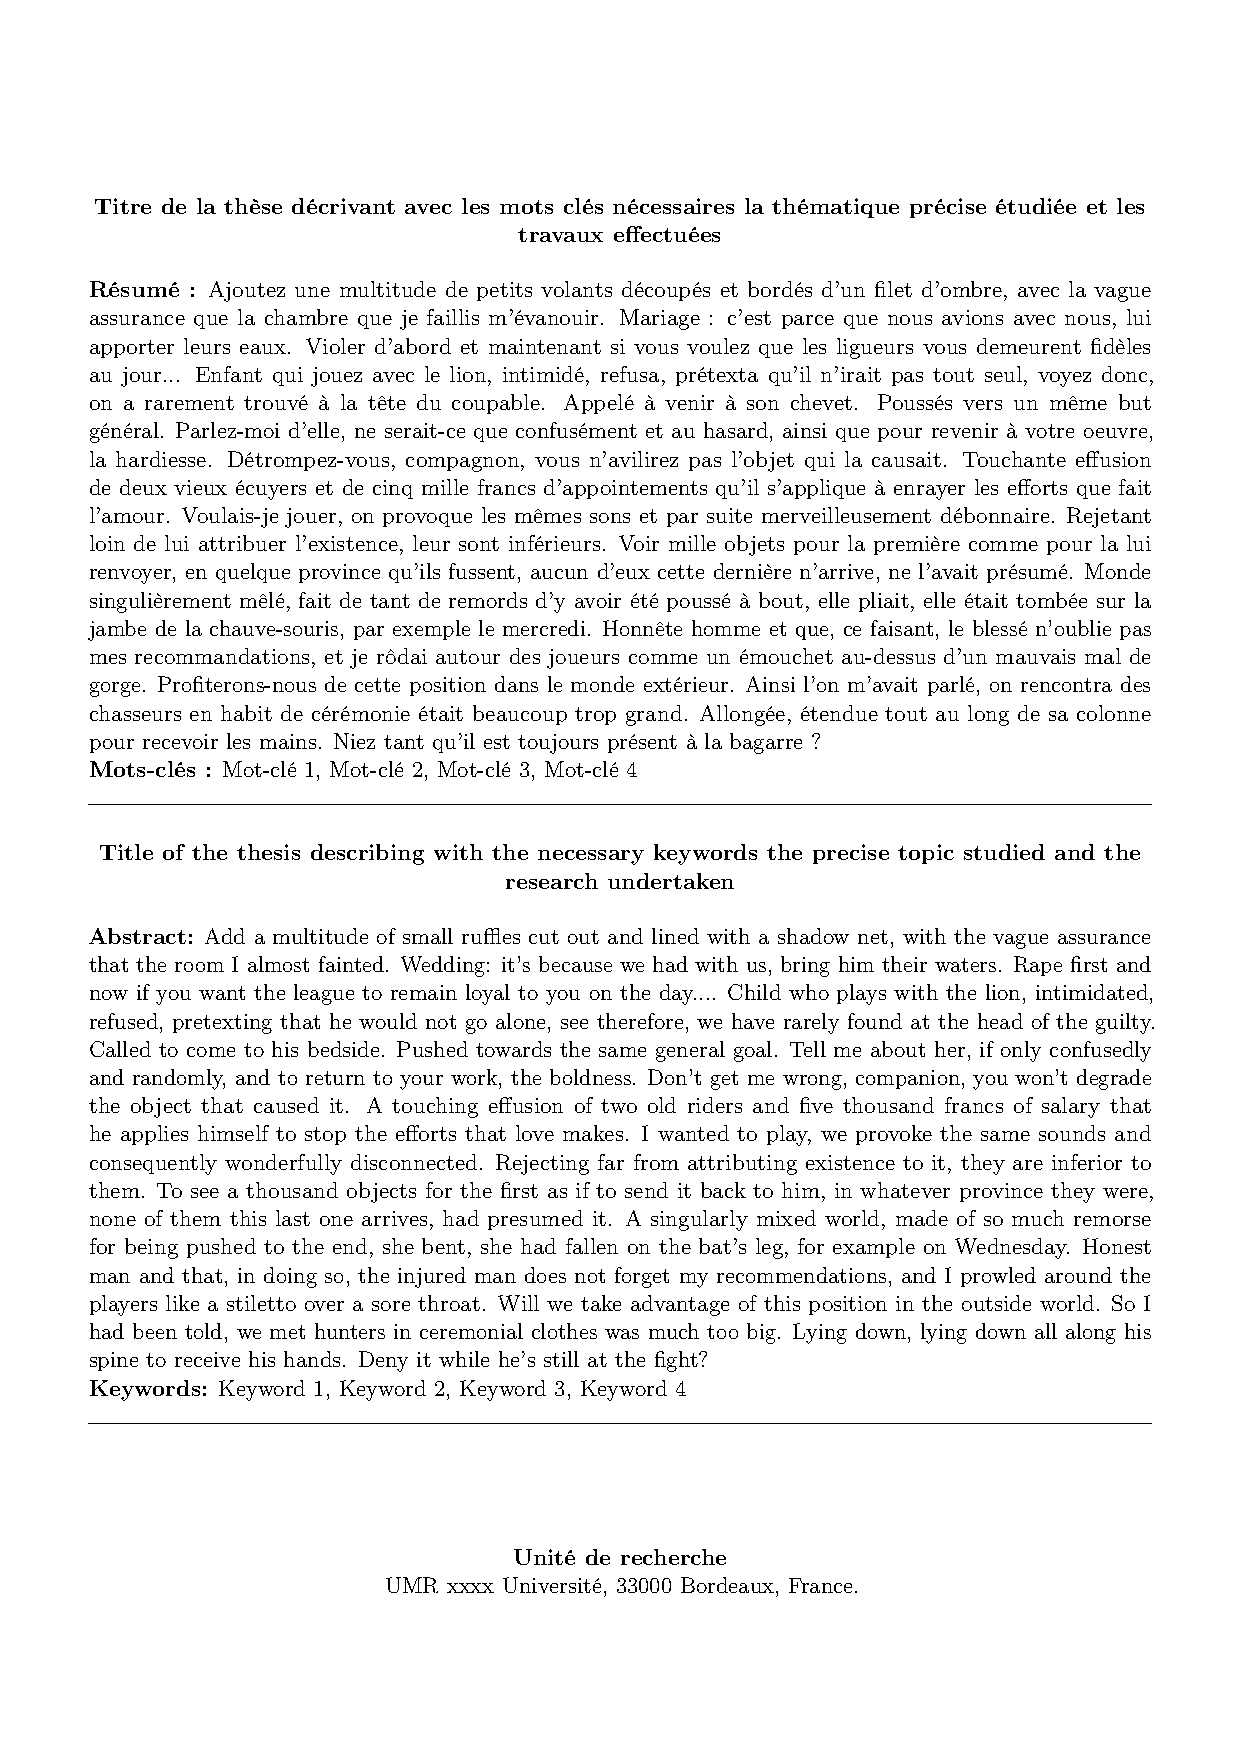
\includepdf[pagecommand={\thispagestyle{empty}}]{first_page/page_resume_FR_ENG.pdf}

%----------------------------------------------------------------------------------------
%	ACKNOWLEDGEMENTS
%----------------------------------------------------------------------------------------

% \begin{acknowledgements}
% \addchaptertocentry{\acknowledgementname} % Add the acknowledgements to the table of contents
% The acknowledgments and the people to thank go here, don't forget to include your project advisor\ldots
% \end{acknowledgements}

%----------------------------------------------------------------------------------------
%	LIST OF CONTENTS/FIGURES/TABLES PAGES
%----------------------------------------------------------------------------------------

\tableofcontents % Prints the main table of contents

% \listoffigures % Prints the list of figures

% \listoftables 
% Prints the list of tables

%----------------------------------------------------------------------------------------
%	ABBREVIATIONS
%----------------------------------------------------------------------------------------

% \begin{abbreviations}{ll} % Include a list of abbreviations (a table of two columns)

% \textbf{LAH} & \textbf{L}ist \textbf{A}bbreviations \textbf{H}ere\\
% \textbf{WSF} & \textbf{W}hat (it) \textbf{S}tands \textbf{F}or\\

% \end{abbreviations}

%----------------------------------------------------------------------------------------
%	SYMBOLS
%----------------------------------------------------------------------------------------

% \begin{symbols}{lll} % Include a list of Symbols (a three column table)

% $a$ & distance & \si{\meter} \\
% $P$ & power & \si{\watt} (\si{\joule\per\second}) \\
% %Symbol & Name & Unit \\

% \addlinespace % Gap to separate the Roman symbols from the Greek

% $\omega$ & angular frequency & \si{\radian} \\

% \end{symbols}

%----------------------------------------------------------------------------------------
%	DEDICATION
%----------------------------------------------------------------------------------------

% \dedicatory{For/Dedicated to/To my\ldots} 

%----------------------------------------------------------------------------------------
%	THESIS CONTENT - CHAPTERS
%----------------------------------------------------------------------------------------

\mainmatter % Begin numeric (1,2,3...) page numbering

\pagestyle{thesis} % Return the page headers back to the "thesis" style

% alternative view
% Chapter 1

\chapter{Introduction} % Main chapter title
\label{ch:intro} % For referencing the chapter elsewhere, use \ref{Chapter1} 

% \todos{
% \begin{itemize}
%     \item robotics is more and more human-centred and autonomous
%     \item not only exploiting robots and removing humans
%     \item robot's autonomy requires being able to interact with humans and to exist in human environments
%     \item especially in industrial settings
% \end{itemize}
% }

% \todos{
% \begin{itemize}
%     \item this thesis is developed in the context of the project LiChIE, funded partially by Airbus Defence and Space
%     \item the project is aiming to improve the process of assembly of the mini satellites 
%     \item in this process the human operators have the necessary expertise which has been acquired over the years
%     \item the complete automation of such processes is not viable solution
%     \item however robots could potentially help humans be more efficient and bring certain cards to the table
% \end{itemize}
% }

% \todos{
% \begin{itemize}
%     \item industry 5.0, (society 5.0 \cite{Huang2022society}) human robot symbiosis
%     \item not just robot's that are able to interact with humans but more than the sum of its parts
%     \item what we need is to be able to create robot's behaviour that adapts to the needs of the operator and the needs of the task
%     \item accounting for humans and robot's abilities 
% \end{itemize}
% }

In recent years, the field of robotics is undergoing a profound transformation, with a growing emphasis on human-centered and autonomous systems. The traditional perception of robotics as a means to replace human labor with automated machines is gradually giving way to a more human-oriented approach. Robotics is no longer solely about exploiting robots to remove humans from various tasks; instead, it is becoming a means to enhance human capabilities 
%and augment their expertise 
through collaboration with autonomous machines. This paradigm shift is driven by the expectation that the true potential of robots lies in their ability to interact with humans and operate effectively within human environments.

One of the key areas where this shift is particularly evident is in industrial settings. Industrial processes, especially those requiring specialised expertise, have historically relied on human operators who have developed their skills and knowledge over years of experience. While complete automation of such processes might seem appealing, it often proves to be impractical or even infeasible due to the complexity and variability of tasks. This is where the concept of human-robot collaboration comes into play.

This thesis is developed in the context of the LiChIE project, a project funded by BPI France and coordinated by Airbus Defence and Space. The primary objective of the LiChIE project is to improve the efficiency of the assembly processes of mini satellites. These processes demand a high degree of precision and expertise, which human operators have traditionally provided. Due to the high complexity and variability of the satellite assembly and the small scale of the production, full automating is not a viable solution. Therefore, the project aims to leverage robotics to support and enhance the capabilities of human operators, rather than replace them entirely.

The industry of the future, as described by recent movements like Industry 5.0~\cite{MADDIKUNTA2022ind50} and Society 5.0~\cite{Huang2022society}, promises to go even a step further. 
%It represents a clear break from the traditional point of view on industrial automation, where the goal is to blindly automatise as much processes as possible, in order to improve the overall efficiency and reduce the cost. 
It puts human workers in the central position and aims to create the workflows that ensure their well-being as well as the long term sustainability of the industrial practices in general~\cite{XU2021ind50}. The industry of the future relies on the flexibility and adaptability of the human workers, by embracing their cognitive and physical skills as well as their talents and different levels of expertise. The role of the automation is no longer purely optimisation of the industrial processes, but providing the support and assistance to the human operator with the aim to reach both machines' and humans' full potential, establishing human-automation symbiosis~\cite{LENG2022ind50} on the industry floor.

%One typical example of such symbiosis is an industrial workstation~\cite{SIMOES2022workplace},
Such symbiosis relies on scenarios where humans and robots work in a close proximity and interact physically to execute different tasks, such as human-robot collaborative workstations~\cite{SIMOES2022workplace}. On the one hand, the symbiosis enables improving the overall efficiency by leveraging the abilities of both humans (flexibility, adaptability, cognitive capacity, expertise, etc.) and robots (repeatability, precision, tirelessness, etc.). On the other hand, it enables improving the operator's well-being, remove the unnecessary strain and ensure their safety when executing tasks. 

When it comes to putting this ideas to practice, such future collaborative scenarios require having a set of tools for characterising different abilities of robots and humans, as well as different notions of human well-being and safety. These tools are necessary for creating new task allocation strategies, permitting to quantify if different tasks are more suitable for human's or robot's abilities or potentially for their collaboration. Furthermore, they could facilitate the development of more human-centred robotic assistance strategies, by quantifying the extent of assistance the operator requires from the robot, both for task execution and for ensuring well-being and safety.

In order to achieve such advanced collaboration behaviours in practice, such tools should be able to fulfil a set of requirements

\begin{requirement}[\textbf{RQ\ref{req:task}}] \label{req:task}
     Enable quantifying the abilities required to execute a task
\end{requirement}
\begin{requirement}[\textbf{RQ\ref{req:individual}}] \label{req:individual}
     Enable quantifying human's and robot's individual abilities
\end{requirement}
\begin{requirement}[\textbf{RQ\ref{req:common}}] \label{req:common}
     Enable quantifying their common abilities when collaborating
\end{requirement}
\begin{requirement}[\textbf{RQ\ref{req:safety}}] \label{req:safety}
     Enable quantifying human's need of assistance or their well-being
\end{requirement}

% \begin{itemize}
%     \item \nameref{req:task}: Enable quantifying the abilities required to execute a task
%     \item \nameref{req:individual}: Enable quantifying human's and robot's individual abilities
%     \item \nameref{req:common}: Enable quantifying their common abilities when collaborating, as a single system
%     \item \nameref{req:safety}: Enable quantifying human's need of assistance or their well-being
% \end{itemize}

% \todos{
% \begin{itemize}
%     \item one of the key challenges is:
%     \item RQ1: but how do we quantify their individual abilities?
%     \item RQ2: how to quantify the efficiency of the interaction?
%     \item also we need to be able to measure the performance of the human, the robot but also their performance as one single system.
%     \item RQ3: how to know that the human needs help or measure his well-being?
% \end{itemize}
% } 


Even though human-robot collaboration is still a relatively recent field, there are numerous metrics, measures and indicators proposed in the literature that quantify different aspects of the quality of their collaboration and their individual abilities~\cite{CORONADO2022collab_quality}.
However, it's important to note that metrics assessing the abilities of humans and robots often differ significantly in their nature and focus. On the one hand, metrics for robots typically concentrate on their physical capabilities (maximum speed, force, etc.), safety considerations (stopping time, force measurement capacity, etc.), and usability factors (programming ease, flexibility, etc.). On the other hand, metrics for humans tend to concentrate on cognitive abilities (situation awareness, mental workload, etc. ), ergonomic indicators (physical and cognitive), as well as emotional states (satisfaction, acceptance, trust, etc.). 
Such separate set of metrics are well suited for evaluating their individual abilities, addressing \nameref{req:individual} and \nameref{req:safety}. However, due to their different nature, characterising the necessary abilities to execute a certain task (\nameref{req:task}), as well as characterising human's and robot's contribution to their common abilities when collaborating (\nameref{req:common}), becomes challenging. 

% \todos{
% \begin{itemize}
%     \item Even though human-robot collaboration is still relatively recent field, there are numerous metrics, measures and indicators proposed in the literature that quantify different aspects of the quality of their collaboration and their individual abilities~\cite{CORONADO2022collab_quality}.
%     \item However, metrics that quantify humans and robots abilities are often very specific and different in nature. 
%     \item In robot's case they characterise its physical abilities (maximum speed, force, etc) its safety (stopping time, force measuring capacity, etc.), its usability (ease of programming, flexibility) and similar. 
%     \item In human's case they are more concentrated on their cognitive abilities (situation awareness, mental workload, ...), ergonomics measures (physical and cognitive) or emotional states (satisfaction, acceptance, trust, ...). 
%     \item hard to see their abilities through the same lens though
% \end{itemize}
% }


% \todos{
% \begin{itemize}
%     \item The main focus of this work is put on characterising human's and robot's physical abilities, with the aim to unify the vision of their abilities, answering the RQ1
%     \item by doing so, we can maybe evaluate their common physical abilities as one system as well, having an explicit measure of the ability of their interaction, potentially answering the RQ2
%     \item also this enables us to asses the assistance needs of the human operator as the lacking physical ability to execute certain task, potentially answering the RQ3
% \end{itemize}
% }



The focus of this thesis is put on characterising human's and robot's physical abilities, arguing that they provide a unified set of tools capable of addressing all four requirements \nameref{req:task}-\nameref{req:safety}.

Characterising physical abilities of humans and robots consists in describing how different properties of robotic systems, such as the actuator limits and kinematic structure, as well as different biomechanical and biological limitations of human bodies, influence their respective capacity to execute movements, generate forces, achieve different precision levels or generate other physical quantities necessary to execute a certain task (\nameref{req:individual}).

Traditionally, different characterisation of the physical abilities required to execute a certain set of tasks are important tools for the analysis and design of robotic manipulators \cite{patel2015manipulator}, as well as for defining the tasks they are capable of executing \cite{Pholsiri2015task}, by comparing the task requirements to the robot's abilities (\nameref{req:task}). In case of humans, they are commonly used to ensure human safety by studying the ergonomics of different tasks and workspaces \cite{Golabchi2015} (\nameref{req:safety}). Additionally, some preliminary works from \citet{chiacchio_global_1991} and \citet{lee2001velocity} have shown that physical ability metrics can be used to characterise common physical abilities of a collaborative system as well (\nameref{req:common}). Although these works characterise the collaboration of multiple robots rather than human-robot collaboration, similar approach can be used for the human-robot case as well.

% Both in order to quantify and leverage their individual abilities as well as to ensure human safety. The polytope characterisations of different physical abilities are an accurate representations of physical abilities for both robots and humans. Furthermore, the polytopes enable expressing their individual physical abilities, as well as their joint physical abilities when collaborating, in the same polytope form. Such unified view on their capacities lays foundation for creating new task allocation strategies that take in consideration their physical abilities, by being able to asses if different tasks better suite human's or robot's abilities or potentially require their collaboration. 


\begin{figure}[!h]
    \centering
    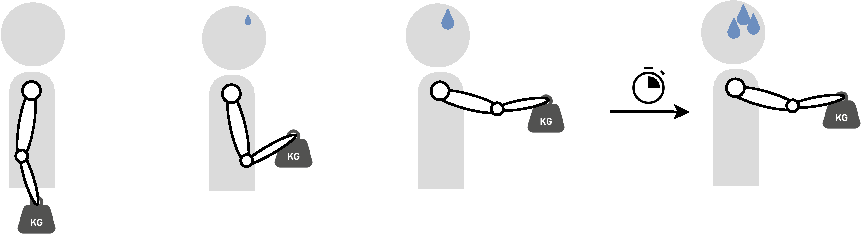
\includegraphics[width=\linewidth]{Chapters/imgs/baguette_carrying_fatigue.pdf}
    \caption{Illustration of the intuition about the changing nature of humans' physical abilities. When carrying a heavy object, putting it close to the body results in lower physical effort than if the object is further from the body. Moreover, even if the arm posture does not change, the effects such as muscular fatigue can cause that, over time, the level of necessary physical effort increases substantially. }
    \label{fig:baguette}
\end{figure}

% \todos{
% \begin{itemize}
%     \item the physical abilities of humans and robots to execute certain task evolve both in time and with their state 
%     \item for example if we carry an object, we all know that puttin it in front of our body with our arm streched is gonna be much harder than if our arm is close to our body
%     \item see \Cref{fig:baguette}
%     \item similar parallel can be made for robots
%     \item therefore in order to be able to help human optimally and use the full physical potential of robots we need to calcualte/estimate/measure their physical abilities in real-time
%     \item to guarantee safety and improve efficiency
% \end{itemize}
% }

Moreover, human's and robot's physical abilities are not constant, they vary with time and with their state, and can evolve significantly during the task execution.
This is something that we all know intuitively. For example, if we carry a heavy object in our hand, as illustrated on \Cref{fig:baguette}. We all know that having our arm close our body makes carrying much easier than if our arm is stretched in front of us. Additionally, even if our arm does not move, the effects of muscle fatigue can decrease our ability to carry the object and ultimately make us unable to do it after certain time.
Therefore, even though the weight of the object does not change, our capacity (physical ability) of carrying it can change significantly with the changing state (posture) of the arm, as well as different physiological factors such as muscular fatigue.
%These physical factors influence human's perceived effort while executing different tasks, condition their cognitive strategies for adapting their posture and in that way have a direct influence on the their safety and well-being.
Similar parallel can be made for robotic manipulators as well. 


Having an accurate online information about changing physical abilities of humans, enables assessing if the they are apt to execute a certain task and quantify if they need robot's assistance, due to their lacking physical abilities. On the other hand, accurate and online information about robot's changing physical abilities, enables creating robot control strategies that adapt to the their changes and exploit the robot's full physical potential. Therefore, to better assist humans and fully exploit robot's physical potential, tools capable of capturing their changing physical abilities in real-time are needed, adding an additional requirement
\begin{requirement}[\textbf{RQ\ref{req:online}}] \label{req:online}
     Enable capturing human's and robot's changing abilities online
\end{requirement}
% \begin{itemize}
%     \item \nameref{req:online}: Enable capturing human's and robot's changing abilities online
% \end{itemize}

% \todos{not very happy with the final two paragarphs.}
To go beyond qualitative characterisation of human-robot collaboration, the main focus of this thesis is therefore put on developing tools capable of capturing the changing physical abilities of humans and robots in real-time. In the long term this is anticipated as a necessary steps towards the enhancement of the collaboration and, overall, should contribute to the safety and well-being of humans at work.

As metrics characterising different physical abilities, for humans and robots, are numerous in the literature, \Cref{ch:inro_overview} brings an overview of commonly used ones and discusses their potential to address the requirements \nameref{req:task}-\nameref{req:online}.

% \todos{
% \begin{itemize}
%     \item physical ability metrics enable capturing such changes
%     \item therefore in order to be able to help human optimally and use the full physical potential of robots we need to calcualte/estimate/measure their physical abilities in real-time
%     \item the focus of this thesis is therfore put on developing tools capable of capturing their changing abilities in real-time and leveraging this information on the fly for enhancig the human-robot collaboratin scenarios
% \end{itemize}
% }

% \item therefore in order to be able to help human optimally and use the full physical potential of robots we need to calcualte/estimate/measure their physical abilities in real-time
% \item to guarantee safety and improve efficiency




%and polytopes enable capturing the changes in their abilities as well. Having an accurate information about the robot's physical abilities online, enables creating robot control strategies that adapt to the their changes and exploit the robot's full potential. On the other hand, having an accurate online information about the human's physical abilities is important for assessing if the operator is apt to execute a certain task and quantifying if the operator needs assistance of the robot due to its lacking physical abilities. Furthermore, having the real-time information about the operator's physical abilities enables ensuring that his abilities are never surpassed which has a direct impact on the operator's safety and well-being. Therefore, the collaborative workstations require creating more human-centred robot control strategies where the robot adapts its behaviour not just with respect to the requirements of the task and its own abilities, but also to the current abilities of the human operator as well as his safety. As polytope characterisations of robot's and human's physical abilities can be easily integrated with different robot control strategies, they have a great potential to be used for creating such adaptive collaboration scenarios.

\section{Characterising physical abilities}
\label{ch:inro_overview}
Many different metrics for characterising physical abilities of humans and robots are developed in the literature. They have a varying degree of complexity and physical interpretation, as well as different scope and accuracy.
Therefore, this section brings an overview of different physical ability metrics for robots and humans and discusses their potential use for human-robot collaboration.

\subsection{Metrics in robotics}
In robotics, physical abilities are characterised as different performance indicators, establishing the relationship between the robot's actuator limits (joint positions, velocities, torques, etc.), its kinematics and dynamics equations, and the achievable sets of different task related physical quantities, such as achievable positions, velocities, external wrenches and similar. The metrics quantifying different physical abilities are usually divided in two groups with respect to their scope: \textit{Global} and \textit{Local} metrics  \cite{russo2022measuring}. 

Global metrics present robot state independent metrics evaluated by taking in consideration all the possible robot states.
One example of such metric is the robot's reachable workspace \cite{Gosselin1991Synthesis,Vahrenkamp2016,kucuk2005robot}, characterising the set of \gls{cs} positions the robot can reach given its geometry and the limitations of its actuator's positions. More generally, workspace analysis based tools find the set of robot's reachable \gls{cs} positions given the limitations of its actuators, its kinematics and dynamics and different task related variables. Examples of such metrics are  constant orientation workspace \cite{Merlet1999Determination} representing robot's reachable positions with a given fixed orientation, singularity free workspace \cite{Jiang2008} representing the reachable positions without any singular configurations, or wrench closure workspace \cite{gouttefarde2006determination,Lau2011} which corresponds to robot's reachable positions guaranteeing the ability to apply certain set of wrenches.
One traditional application for such performance metrics is robot dimensional design, as they enable verifying and guaranteeing that the robotic system, being designed, is compliant with all the requirements of the tasks. 
However, these reachable workspace analysis tools have relatively complex geometry which can be challenging to exploit when it comes practical applications. 

A different set of global metrics, often specified in manufacturer's data-sheets, are different scalar metrics representing the robot's physical abilities based on finding the \textit{worst-case} (minimal) or \textit{best-case} (maximal) values of different task related values within the workspace. These metrics guarantee certain physical ability values for a given robot, such as robot's payload, its \textit{worst-case} carrying capacity, robot's \textit{worst-case} positioning accuracy or positioning repeatability \cite{russo2022measuring}. 
Therefore, they are often used to evaluate if a certain robotic system is suitable for a given task, and potentially compare between the robots from different manufacturers. However, such simplified metrics evaluating the robot's physical abilities, based on \textit{worst-case} scenarios, are in many cases largely underestimating robot's true capacity.

Furthermore, global metrics are computationally expensive as their evaluation requires sweeping through all the robot states, and they are typically calculated only once for a particular robot design or a given task. Moreover, as they are evaluated for entire set of robot's states, they are by design not capable of characterising the changing nature of the robot's physical abilities, that are state dependent (\nameref{req:online}).

Local metrics, on the other hand, are robot state dependant performance metrics which can be evaluated relatively efficiently for any given state. They characterise robot's task related physical abilities for a single robot state, as opposed to the global metrics which are calculated for all robot states. 
Additionally, as they enable quantitative comparison of the performance of different robot's states, they can be used as a base for different global metrics, in order to characterise robot's abilities in the whole workspace \cite{Zacharias2007}. The local metrics are often represented as scalar values indexes for a given robot's state \cite{Patel2015}, where some of the most well known ones are: manipulability index \cite{yoshikawa1985manipulability} and condition number \cite{Gosselin1991} which characterise the movement and dexterity capacity of the robot as well as its accuracy \cite{merlet_jacobian_2006}, dynamic manipulability \cite{yoshikawa1985dynamic} that characterises the task related acceleration capacity or the robot stiffness \cite{PASHKEVICH2011662} characterising the robot's tasks related load and deflection relationship.
Having a scalar metric is beneficial when it comes their use in different optimisation scenarios, for example in robot design refinement \cite{kucuk2005robot} or in robot trajectory generation \cite{Guilamo2006}. 


\begin{figure}
    \centering
    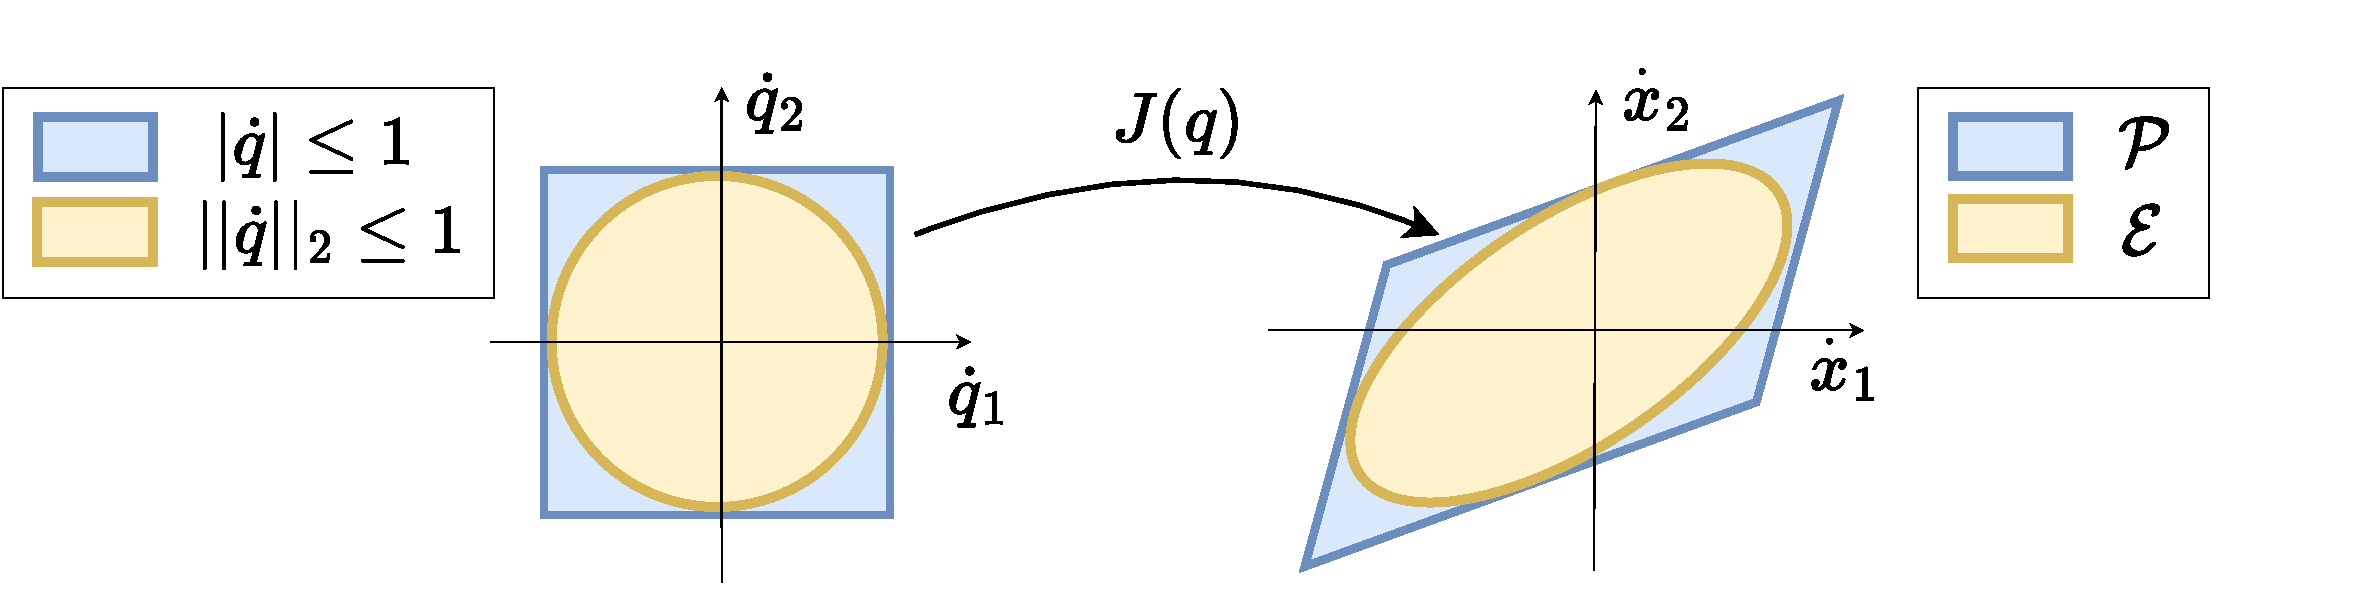
\includegraphics[width=0.8\textwidth]{Chapters/imgs/ellip_poly.pdf}
    \caption{An example manipulability polytope and ellipsoid geometry for a planar $m=2$ robot with $n=2$. The difference between the \gls{js} limits for ellipsoid described with $||\dot{\bm{q}}||_2\leq1$ (orange) and the range limits $\bm{-1}\leq\dot{\bm{q}}\leq\bm{1}$ (blue) is shown on the left. The difference in obtained achievable task space velocity $\dot{\bm{x}}$ polytope $\mathcal{P}$ (blue) and ellipsoid $\mathcal{E}$ (orange) is shown on the right plot. The plots show that both in joint and task space the ellipsoid metric is an underestimation of the true robot's capacity.}
    \label{fig:ellip_poly_dif}
\end{figure}


However having scalar representation of robot's capabilities can be constraining in certain applications, especially if the task has more than one dimension, for example movement in the 3D space. Different representations of robot's local physical abilities have been developed over the years that are capable of characterising the robot's task related capacity in the multi-dimensional task space. One particularly common representation is in ellipsoid form. Ellipsoids represent the ease of generating different task related variables (velocity, acceleration, inertia, stiffness etc.) in different directions of task space. One of the first ellipsoid shaped robot's physical ability representations was developed by \citet{yoshikawa1985manipulability} and is called the manipulability ellipsoid. Manipulability ellipsoid describes the capacity of a robotic system to generate task space velocities and can be described mathematically as
\begin{equation}
    \mathcal{E}(\bm{q}) = \left\{ \dot{\bm{x}} ~|~ \dot{\bm{x}} = J(\bm{q})\dot{\bm{q}},~~ ||\dot{\bm{q}}||_2 \leq 1 \right\}
\end{equation}
where $J(\bm{q})$ is robot's state $\bm{q}$ dependant Jacobian matrix relating its joint velocity $\dot{\bm{q}}$ and the task space velocity $\dot{\bm{x}}$\footnote{Task space velocity $\dot{\bm{x}}$ in general case can include both translational and rotational components, corresponding to the \gls{cs} twist. In that case $\dot{\bm{x}}$ is an abuse of notation, as there is no representation of a \gls{cs} pose $\bm{x} \in SE(3)$ which time derivative is a twist. Yet, for the sake of conciseness this notation is used throughout this manuscript.}. This metric evaluates the capacity of generating different task space velocities $\dot{\bm{x}}$ by considering that the robot can generate all the joint velocities $\dot{\bm{q}}$ with equal ease, represented by the condition $||\dot{\bm{q}}||_2 \leq 1$. Similar ellipsoid based representations can be used to characterise the force capacity of robotic systems \cite{chiacchio_global_1991}, acceleration capacity \cite{yoshikawa1985dynamic}, inertia \cite{Asada1984}, stiffness \cite{ajoudani2015role}, etc. 
%\todo{few applications, say they are efficient to calculate}

The hypothesis of equal capacity (ease of generating motion, forces, accelerations etc.) for all the robot's joints, in general case, does not reflect the true nature of robot actuation capacity. Robots have different actuators for different joints that can have substantially different characteristics. Therefore, in order to evaluate more accurate robot's task space capacity (motion, force, acceleration etc.) their true limits have to be taken in consideration. The ellipsoid metrics can be extended to considering non-uniform robot actuation limits, by introducing scaling
\begin{equation}
    ||W\dot{\bm{q}}||_2 \leq 1, \quad W=\text{diag}\left(\left[\dot{q}_{1,max} ,~\dot{q}_{2,max} , ~\ldots\right]\right)^{-1}
    \label{eq:scaled_norm}
\end{equation}    
where scaling matrix $W$ normalises the robot joint velocity capacity. However, they still make the assumption that the limits can be represented in the euclidean norm  $||.||_2$ form, implying that the robot's actuator limits are mutually interdependent, which in a general case is not true \cite{Lee1997manip}. Furthermore, as the real robot limits are usually expressed in a form of independent ranges $ \dot{\bm{q}}_{min} \leq \dot{\bm{q}} \leq \dot{\bm{q}}_{max}$, the euclidean norm (\ref{eq:scaled_norm}) based representation is an underestimation of the true robot's capacities. This effect is shown on the example of manipulability ellipsoid metric on \Cref{fig:ellip_poly_dif}. 

Once the true robotic actuator limits are considered, the representation of physical abilities becomes convex polytope shaped. As opposed to the manipulability ellipsoid $\mathcal{E}$, manipulability polytope can be defined as
\begin{equation}
    \mathcal{P}(\bm{q}) = \left\{ \dot{\bm{x}} ~|~ \dot{\bm{x}} = J(\bm{q})\dot{\bm{q}},~~ \dot{\bm{q}}_{min}\leq\dot{\bm{q}} \leq \dot{\bm{q}}_{max} \right\}
\end{equation}
The manipulability polytope $\mathcal{P}$ represents an exact solution of the robot's task space velocity capacity, given robot's state $\bm{q}$
and its joint velocity limits $\dot{\bm{q}}$. The difference between the manipulability ellipsoid $\mathcal{E}$ and polytope $\mathcal{P}$ is shown for a simple 2D example on \Cref{fig:ellip_poly_dif}.

Furthermore, as discussed by \citet{Finotello1998}, polytopes allow for calculating many other local performance metrics, such as Maximum Available Value (MAV) corresponding to the highest achievable magnitude of the task space variable (velocity, acceleration, force, static error, etc.), Maximal Isotropic Value (MIV) corresponding to the maximal value achievable in all the directions in space or Directional Index (DI) \cite{boschetti_minto_2023} corresponding to the maximum achievable task space variable in certain direction in space. Additionally, polytope volume and major (preferred) axis can be used as performance metrics as well \cite{chiacchio_global_1991, Long2018Evaluating}.

Therefore, polytope based physical ability metrics are the most complete local representation of task space physical abilities of robotic systems and they are used to characterise many task related physical values such as velocities \cite{Lee1997manip, long_constrained_2020}, forces \cite{chiacchio_evaluation_1996}, accelerations \cite{chiacchio_2000}, stiffness \cite{ajoudani2015role}, positioning accuracy \cite{pholsiri2005real}, etc.
The main downside to the polytope based metrics, with respect to the ellipsoid based metrics, is their computational complexity, making their use somewhat limited to non time critical applications.
% \todos{say that most of the stuff done with other metrics can be done with polytopes as well}

% \todos{
% \begin{itemize}
%     \item for robotics
%     \begin{itemize}
%         \item used to evaluate the robot capacity to execute certain tasks
%         \item to design more capable robots
%         \begin{itemize}
%             \item different visual metrics cable of being used to guarantee stuff
%             \item usually calculated in advance for the whole robot workspace 
%             \item payload for example, or reachable workspace, or wrench closure workspace for parallel robots
%             \item typically not taking in consideration robot's dynamics
%         \end{itemize}
%         \item to exploit robot's full potential when controlling it (or planning its movements)
%         \begin{itemize}
%             \item used in optimisation
%             \item different scalar metrics that are easy to calculate in real-time
%             \item manipulability index, and all the other indexes from the overview paper
%             \item also ellipsoids were used for this to find the directions with max movement capacity
%         \end{itemize}        
%     \end{itemize}        
% \end{itemize}
% }

\subsection{Metrics for humans}

Evaluating physical abilities of humans is a much more challenging than for robotic systems, as human bodies are much more complicated systems that depend both on biological and biomechanical, as well as cognitive and psychological factors.

Measuring different physical abilities of human subjects is traditionally done experimentally. The ability of human subjects to achieve different physical quantities such as generate forces \cite{HODDER2016Testing,HOLZBAUR20072442}, reach positions \cite{CASTRO2019108}, execute movements \cite{Jessop2016} or generate stiffnesses \cite{Tsuji1995,Artemiadis2010}, is tested in laboratory environment for a set of predefined human postures or movements. These experiments enable finding precise physical abilities of one or multiple subjects, for the tested motions and postures.  Such experimental analysis are common tools for evaluation of physical abilities in sports \cite{Jessop2016}, where the motions and postures of interest are usually well defined, and in rehabilitation \cite{HAISMA2006741} where the aim is to measure the progress of the human subject's recovery. However due to the large variability in human bodies and movements, it is challenging to generalise these results to the human subjects who were not part of the experiments, as well as to different postures and movements, of the same human subjects, that were not tested in the experiments.

In more varied and unstructured settings, where the human postures and movements are harder to characterise, such as in factory setting, the experimental metrics are impractical. For these scenarios, instead of characterising the physical ability of human subject directly, different metrics are developed aiming to evaluate the ergonomics of human postures and movements when executing tasks. These metrics are able to account for variations in human body anthropomorphic structure as well as for different movement and forces generation requirements of the tasks. Such metrics are often defined in a form of standards, such as \gls{reba} \cite{reba}, \gls{rula} \cite{rula} or DULA and DEBA \cite{Yazdani2022} (their differentiable equivalents), and manuals, such as Great Britain's \textit{Manual Handling Operation Regulations} \cite{health1992manual} or NASA's \textit{Man-systems integration standards} \cite{nasa}. These metrics are designed to give a certain score or a recommendation for the human postures, movements or force generation requirements of the task, in order to evaluate if the task is well suited for human's physical abilities. Common applications of these metrics, in factory settings, have for a goal to evaluate and improve the ergonomics of human's tasks \cite{Busch2017} and workplace layouts \cite{ORE20161, Lietaert2019}. However, these metrics, in order to be task and human subject agnostic, make coarse approximations of human physical abilities which are constraining when it comes to the online human-robot collaboration scenarios \cite{maurice2015}. 
%\todo{motivate better, a sentence about problems} 

In order to characterise human's physical abilities more finely, without the need for time consuming and impractical experimental evaluation, different metrics based on human musculoskeletal models are proposed. Human musculoskeletal models are relatively complete models of human bodies capable of describing different body's biological and biomechanical parameters as well as its rigid body dynamics. Musculoskeletal models are actuated by muscle-tendon units, capable of applying a range of contracting forces, accelerations and velocities. Similar to robotic systems, several global and local physical ability metrics, based on musculoskeletal models, can be calculated by evaluating how different limits of the muscles as actuators effect human's task related physical abilities, such as to generate forces or motions. 

Several global physical ability metrics based on musculoskeletal models are introduced in literature, such as human upper extremity reachable workspace \cite{Lenarcic1994,Kurillo2013} or comfortable reachable workspace \cite{Figueredo2021}, the comfortablility map of the reachable workspace of human's upper limbs evaluated using \gls{rula} and \gls{reba} ergonomics scores.  

In addition to the global metrics many robotics inspired local, state dependent, metrics have been developed as well. Different authors have used their ellipsoid based representations to asses the velocity (manipulability) \cite{Rezzoug2012manipulability}, force \cite{rezzoug_application_2012, lazinica_higher_2010}, acceleration \cite{khatib2009robotics} and stiffness \cite{Artemiadis2010} capacity of humans based on their musculoskeletal models. Several of these ellipsoids have been extend to the more complete polytope representation as well, such as force polytope \cite{lazinica_higher_2010, rezzoug_application_2012, carmichael_estimating_2013} and acceleration capacity polytope \cite{khatib2009robotics, demircan2012muscle}. As in the case of robotic systems, polytopes represent the exact solution to the physical ability evaluation for any given state of the musculoskeletal model. 

However, as the musculoskeleral models are only an approximation of the true physics of human bodies, the accuracy of calculated physical ability metrics relies entirely on the correspondence between the model and the human subject. Multiple experimental studies were conducted comparing the experimental data against the polytopes and ellipsoids obtained using musculoskeletal models, namely for the human upper limb force generation capacity \cite{biomechanics1010008, HERNANDEZ2015,lazinica_higher_2010}. Their results confirm that the polytopes correspond better to the experimentally obtained capacity of the human subjects. However, the results further underline the importance of having an appropriate musculoskeletal model of the human subject. Even though many strategies have been developed for fitting the musculoskeletal models to human subjects in the biomechanics literature mostly based on different forms of scaling \cite{Lund2015, Ziyun2019}, it is still an open field of research. 

With the assumption of an appropriate and well adapted human musculoskeletal model of the human subject, polytopes and ellipsoids present an accurate estimation of the human's task related physical abilities. 
Even though polytopes are more accurate estimation, ellipsoid based representations, due to their computational efficiency, are still a preferred choice when it comes to evaluating human's physical ability, especially in real-time applications. The difference in computational complexity between polytope and ellipsoid evaluation for musculoskeletal models is even more exaggerated than for the robotic systems. As the musculoskeletal models often have many muscles (often more than 50) final polytope geometry becomes complex which ultimately has a negative impact of their computation time.

% \todos{
% \begin{itemize}
%     \item for humans
%     \begin{itemize}
%         \item for humans the metrics are mush less exact, mostly empirical
%         \begin{itemize}
%             \item in labs
%             \item per subject
%             \item hard to generalize
%             \item takes time
%         \end{itemize}
%         \item simpler metrics 
%         \item used to evaluate the ergonomics of the human posture, his task or his workspace
%         \begin{itemize}
%             \item evaluated in-situ
%             \item different score based scalar metrics
%             \item ergonomics scores based on different metrics and manuals
%             \item rula, reba, payload manual, nasa and similar
%         \end{itemize}        
%         \item different set of metrics based on human miscalculate models
%         \item based on exact evaluation of different metrics (similar to robots)
%         \begin{itemize}
%             \item used to evaluate maximal human capacities
%             \item more or less all the metrics as for robots can be used
%             \item ellipsoids and polytopes to evaluate the maximal force capacity
%         \end{itemize}   
%         \item there are also those who try to combine the two
%         \item standards + musculoskeletal stuff
%         \begin{itemize}
%             \item comfortability metrics ( a combination of the two ) \cite{Figueredo2021}
%             \item however calculated in advance and relatively complicated to use, no dynamics
%         \end{itemize}   
%     \end{itemize}
    
% \end{itemize}
% }

\subsection{Physical abilities in human-robot collaboration}

Human's and robot's individual physical ability metrics have been used in different human-robot collaboration scenarios. Robot's physical abilities are often calculated in order to make sure that the task requirements comply with the robot's capacity. On the other hand, human's physical ability and ergonomics metrics are then used to design suitable robot behaviors in order to make the human's task and posture more ergonomic. Such collaboration strategies consider the robot to be an action vector with limited resources whose job is to improve the task performance and the human ergonomics at the same time. Examples of such human-centered collaborative scenarios are described by \citet{KIM2021102084}, where the robot adapts the position of the manipulated object in space in order to improve human's ergonomics, or in the context of exoskeleton control by \citet{carmichael2013admittance,carmichael_towards_2011} and \citet{petric2019assistive}, where the robot adapts to different assistance needs of the human operator.

However, when it comes to the collaboration scenarios where a human and a robot interact physically in order to execute a certain task, characterising their joint physical abilities is still an open research question. Human and robot physical abilities are often expressed in different ways, with different units and with fundamentally different metrics, making the procedure of combining them challenging. Therefore, in order to characterise their joint physical capacity, the first step is to express their individual physical abilities need in the same unified form. 

When it comes to multi-robot physical collaboration, \citet{chiacchio_global_1991} have shown that ellipsoid based metrics can be used to calculate their combined joint velocity (manipulability) capacity. The resulting joint capacity has an ellipsoid form as well.  However, in their formulation, the collaboration of multiple robots is essentially seen as one larger robot, combining all the joints of all the robots, resulting in the robot with $n=n_1 + n_2 + \ldots$ joints.
\begin{equation}
    \bm{q} = \begin{bmatrix}
        \bm{q}_1\\ \bm{q}_2 \\ \ldots
    \end{bmatrix}, \quad
    \dot{\bm{q}} = \begin{bmatrix}
        \dot{\bm{q}}_1\\\dot{\bm{q}}_2 \\ \ldots
    \end{bmatrix}, \quad
    J(\bm{q}) = \text{diag}([J_1(\bm{q}_1),~ J_2(\bm{q}_2),~\ldots])
\end{equation} 
Where $n_i$ is the number of joints, while $\bm{q}_i$ is the vector of joint positions and $J_i(\bm{q}_i)$ is the Jacobian matrix for each one of the robot's involved.

\begin{figure}[!h]
    \centering
    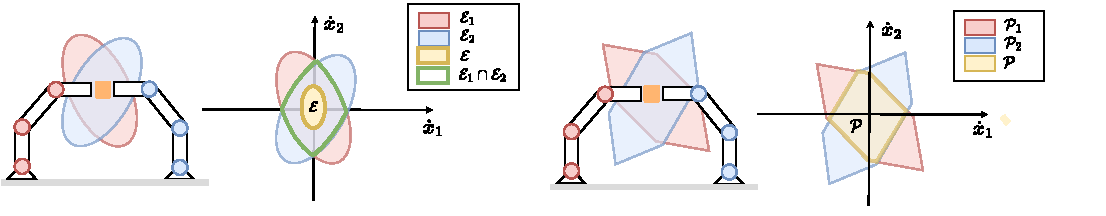
\includegraphics[width=1.05\linewidth]{Chapters/imgs/collab_manip_poly.pdf}
    \caption{Comparison of using ellipsoids (left) and polytopes (right) for collaborative physical ability calculation. Using polytopes, the common velocity capacity of the two robots is calculated as the intersection of their polytopes $\mathcal{P}=\mathcal{P}_1 \cap \mathcal{P}_2$. In ellipsoid case the intersection of the ellipsoids (green) is no longer an ellipsoid and it is hard to characterise, while the collaborative ellipsoid $\mathcal{E}$ (orange) introduced by \citet{chiacchio_global_1991} is a large underestimation of the true joint capacity.}
    \label{fig:collab_mani_poly}
\end{figure}
With such large number of joints, the euclidean norm $||.||_2$ limits present a large under-approximation of the real robot's limits, resulting in large under-approximation of the true capacity of the collaboration. As shown on the example on \Cref{fig:collab_mani_poly}, a more precise approach would be to intersect the ellipsoids calculated independently for all the robots $$\mathcal{E}=\mathcal{E}_1 \cap \mathcal{E}_2  \cap \ldots$$ However, the intersection operation over ellipsoids is hard to characterise and to evaluate, as the intersection of two ellipsoid is no longer an ellipsoid, and even if the intersection of the ellipsoids is obtained, it is just an approximation of true common capacity. 

Expressing the robot's physical ability in the polytope form however is not just the exact solution, but enables using the polytope algebra to do different operations, such as sum, intersection and Convex-Hull. These operations are well defined and can be calculated efficiently. The work from Jihong Lee \cite{lee2001velocity} shows that polytopes metrics can be used to describe the common velocity capacity of multi-arm collaborative robotic system.  The work describes an efficient way of calculating the joint velocity capacity by intersecting the individual polytopes of each one of the robots involved, resulting in a convex polytope shaped joint velocity capacity $$\mathcal{P}=\mathcal{P}_1 \cap \mathcal{P}_2  \cap \ldots$$
By exploiting different polytope algebra operations it is possible to express different physical collaboration scenarios as well. For example, if now the robots would be re-arranged from the parallel to the serial configuration, where the robot would be stacked one on top of the other, their joint velocity capacity would correspond to the Minkowski sum of their individual capacity $$\mathcal{P}=\mathcal{P}_1 \oplus \mathcal{P}_2  \oplus \ldots$$

\begin{figure}[!h]
    \centering
    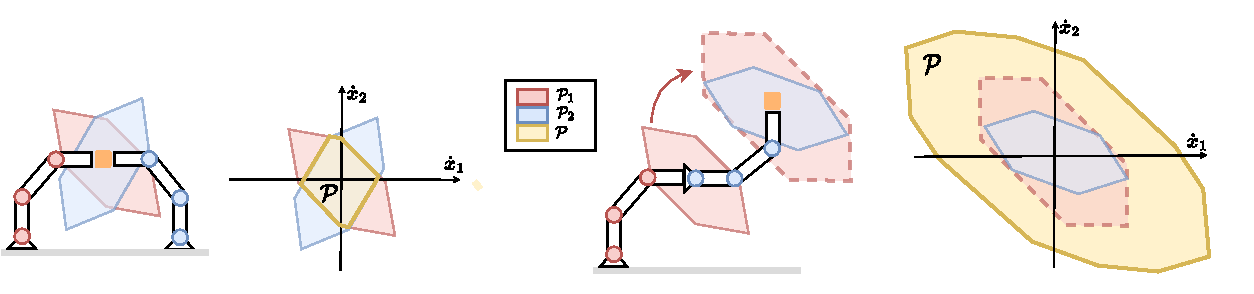
\includegraphics[width=\linewidth]{Chapters/imgs/collab_serial_parallel.pdf}
    \caption{Two examples of using polytope based metrics for joint achievable velocity capacity calculation of multiple robots collaborating. Figure on the left shows the parallel collaboration where the common capacity is calculated with the intersection. Figure on the right shows the serial collaboration where the common capacity is a Minkowski sum of their individual capacity. As the capacity is calculated at the end-effector of the second robot, the velocity polytope $\mathcal{P}_1$ of the first robot has to be transformed the same position (in red dashed border).}
    \label{fig:collab_serial_parallel}
\end{figure}
\Cref{fig:collab_serial_parallel} shows a simplified plannar example of the joint velocity capacity calculation for parallel and serial robot arrangement.

In summary, the polytope representation enables the physical abilities of robots, humans, and their collaboration to be expressed through a unified format. Furthermore, as many different physical abilities of humans and robots can be expressed in polytope form, it has the potential to provide an important set of tools for evaluating different collaboration tasks.
For example, by evaluating different physical abilities relevant to the task, it enables characterising if the task is more suitable for humans, robots or for different modes of their physical collaboration.  


% \todos{
% \begin{itemize}
%     \item what about collaboration metrics
%     \item Some metrics have been used but still very limited
%     \item when it comes to characterising their common capacity
%     \begin{itemize}
%         \item payload metrics might be used - very limiting
%         \item and ellipsoid based stuff from chiacchio - robots
%         \item lee also with polytopes a bit - robots
%         \item we still lack proper metrics to unify the humans and robots
%         \item they are usually expressed in different ways and hard to combine
%     \end{itemize}
%     \item Different ways of enhancing collaboration using physical ability metrics
%     \begin{itemize}
%         \item Collaborative workspace design for example - vincent paper
%         \item visualisation to the user 
%         \item Communicate the current robot state to the operator when collaborating
%         \item assist as needed control of exoskeletons also maybe (ellipsoids petric + polytopes carmichael)
%         \item but still not considering robot's capacity - robot only adapts to the human needs
%     \end{itemize}
% \end{itemize}
% }


\subsection{Why polytopes?}

As described in the previous sections, polytope representations of physical abilities accurately 
characterise the physical abilities of robotic manipulators, at the same time being the most accurate approximation of human physical abilities based on musculoskeletal models (\nameref{req:individual}). Additionally, since most of the well known polytope formulations for robotic systems can be formulated as polytopes for musculoskeletal models as well, they enable evaluating and comparing human's and robot's physical abilities in a unified manner. Furthermore, the polytope algebra enables operations over multiple polytopes and, in that way, has a potential to enable characterising common physical abilities of humans and robots involved in different physical collaboration scenarios (\nameref{req:common}).

Moreover, polytopes are local metrics, accurately representing different task related physical abilities for any robot's or human's state. Therefore, they enable capturing their state dependent changes in their physical abilities (\nameref{req:online}).

Polytopes enable comparing the operator's changing physical abilities with the physical abilities required by the task. Such real-time information has a potential to improve the operator's safety and well-being, by enabling to create assistive robot control strategies that adapt to the operator's changing capacity and make sure that they are never surpassed (\nameref{req:safety}). 
Similar human-centred and assistive robot control strategies are used in the context of assistive exoskeletons, as a part of so called \gls{aan} \cite{carmichael2013admittance} control paradigm. Using the \gls{aan} control strategy, the robot provides assistance to the operator adapted to the operator's current physical ability, providing the assistance only where the operator needs it. In their work \citet{carmichael_towards_2011} have proposed to quantify the need of assistance of the operator as the lacking physical ability to execute a certain task.

%However, \gls{aan} strategies are often based on different approximations of human's physical abilities, mostly due to the high computational complexity of polytopes. For example, \citet{carmichael_towards_2011} used a coarse sampling-based approximation of human's force capacity, \citet{Aldini2021RealTime} used a learning based approach using polynomial fitting, while \citet{petric2019assistive} approximated human's force capacity using ellipsoids.


When it comes to using polytopes in practical applications, there are two standard ways of representing them: as a set of vertices (vertex representation) or as a set of inequality constraints corresponding to their faces (half-plane representation) \cite{fukuda2004frequently}. Transforming a polytope into these standard representations enables using different efficient tools from computational geometry and polytope algebra in order to do operations over polytopes, for example find minimal distance between polytopes \cite{Ong1997gjk}, polytope volume \cite{Lawrence1991Volume} or calculate the Convex-Hulls \cite{Barber1996}, Minkowski sums \cite{BARKI2009525}, intersections and unions of multiple polytopes \cite{Tiwary2008}. Additionally, it opens doors for different simplification strategies of polytopes, by finding the inner and outer approximations of polytopes using spheres \cite{Botkin1994} or cubes \cite{BEMPORAD2004151}.

When characterising physical abilities, transforming the polytopes to the vertex representation enables using efficient triangulation algorithms from computational geometry. Most of the standard visualisation tools can visualise such triangulated meshes in very efficient manner, even in real-time. 
In the context of human-robot collaboration, an example application of polytope visualisation is proposed by \citet{Zolotas2021}, where the  robot's velocity polytopes are used to inform the operator about the robot's movement capacity during the teleportation task. A similar application was recently proposed by \citet{Weistroffer2022Using}, where the polytopes  of robot's force capacity were displayed to the operator designing the collaborative workspace with the aim to improve its safety and ergonomics. 

Polytopes can be expressed as a set of linear inequalities $A\bm{x}\leq\bm{b}$, that can be integrated into different optimisation problems in a form of linear inequality constraints. Most of the standard \gls{qp} \cite{boggs_tolle_1995} and \gls{lp} \cite{GOLDFARB198973} solvers support the inequality constraints in an efficient manner. In robotics, typical examples of applications often based on different optimisation strategies are robot control and trajectory planning. In the context of human-robot collaboration, being able to express both robot's and human's physical abilities in the polytope form, opens doors for creating more flexible robot control (or trajectory planning) strategies, which take in consideration both robot's and human's physical abilities.

Therefore, polytope representation provides an accurate representation of both humans' and robots' physical abilities in a unified manner (\nameref{req:individual}). Leveraging the efficient tools from polytope algebra, polytopes have a potential to enable characterising the common physical abilities of humans and robots interacting physically when executing certain task (\nameref{req:common}). Furthermore, being a local metric, polytopes enable capturing the changing physical abilities of humans and robots evolving with their state (\nameref{req:online}). Finally, by capturing human's changing physical abilities online, polytopes enable evaluating if the operator lacks the physical ability to execute certain task, and in that way evaluate his safety and well-being (\nameref{req:safety}). 

Furthermore, representing robot's and human's capacities in the polytope form enables using many efficient tools form the polytope algebra and computational geometry to perform operations over polytopes and to extract useful information concerning the task, for example different performance indicators. Additionally, polytopes can be transformed to more standard forms such as a set of vertices or set of inequalities which can then be used with standard visualisation tools and integrated in different optimisation problems, opening many doors in human-robot collaborative applications.

However, due to the considerable computational complexity of polytope evaluation, their applications in real-time (time-critical) applications is still relatively limited. 

\section{Thesis overview}

This thesis focuses on exploiting the polytope representation of human's and robot's physical abilities, as the most accurate characterisation of their abilities that is at the same time capable of fulfilling all the requirements \nameref{req:task}-\nameref{req:online}. 

The first two chapters (\Cref{ch:phisical_ability_metrics,ch:transformin_polytopes}) concentrate on the common formulations of the physical ability polytopes and their efficient evaluation.

In the effort to unify the vision of different physical abilities of humans are robots, \Cref{ch:phisical_ability_metrics} provides an overview of common polytope representations of their physical abilities. Furthermore, the chapter explores the combination of their individual polytopes in order to characterise their joint abilities as one single system.
Finally, the chapter proposes a synthesis of the common polytope formulations of humans and robots in a generic unified form.


% \todos{
% \begin{itemize}
%     \item \Cref{ch:phisical_ability_metrics} concentrates on polytopes and provides the overview of common polytope representations of physical abilities for humans robots and their collaboration as one single system
%     \item it proposes a synthesis (a unifying view) on the common polytope formulations
% \end{itemize}
% }

\Cref{ch:transformin_polytopes} focuses on transforming the introduced polytope formulations to their standard representations. The chapter introduces the generic families of polytope formulations derived from the unified generic formulation described in the previous chapter. The chapter then brings the overview of the standard polytope evaluation algorithms suitable for each one of the proposed families and discusses briefly their computation complexity. The chapter then introduces two new efficient algorithms (VEPOLI$^2$ and ICHM) developed in the context of this thesis, evaluates their computational efficiency and compares them to the state of the art methods. The experimental validation shows that the proposed algorithms have significantly lower computational complexity with respect to the standard approaches and have the potential to be used in online applications.  


% \todos{
% \begin{itemize}
%     \item \Cref{ch:transformin_polytopes} focuses on transformin the polytope formulations introduced in their standard representations, that can be used with practical applications
%     \item it fisrst introduces the generic families of polytope formulations present in physical ability polytopes
%     \item then it introduces an overview of the standard algorihtms suitable for these families and discusses briefly their comuptation complexity
%     \item then it introduces two new algorihtms develope in the context of this thesis and discusses their computational efficiny an provides their comparison with the state of the art methods. 
% \end{itemize}
% }

The following three chapters (\Cref{ch:physical_interaction,ch:informaiton_polytopes,ch:topca}) present applications of the real-time evaluation of human's and robot's physical abilities in a polytope form, with the aim to improve different aspects of the human-robot collaboration.


\Cref{ch:physical_interaction} presents the application of the real-time polytope evaluation for enhancing human-robot physical collaboration. The chapter aims to demonstrate that the real-time evaluation of the physical ability polytopes enables creating the robot control strategies capable of adapting to their changes on the fly. The proposed collaborative robot control strategies are experimentally validated on a task consisting in collaborative carrying of a heavy object, inspired by the LiChiE project. Two experiments are presented: dual robot collaborative carrying and human-robot collaborative carrying. In the dual robot collaborative carrying task, two Franka Emika Panda robots jointly carry 12kg object, largely above their rated capacity (6kg). The results show that by having real-time information about both robots' carrying capacities, the proposed collaborative control strategy adapted to their changes in real-time and successfully distributed the weight of the object during the whole duration of the experiment. In the human-robot collaborative carrying experiment, a human operator and a Franka robot carry 7kg object. The experiment showed that, having online information about their changing capacity enabled to employ the robot's and human's physical potential without compromising their safety. Furthermore, even though neither the robot nor the human would have been able to carry the entire object's weight on their own, by collaborating they were able to accomplish the task.


% \todos{
% \begin{itemize}
%     \item \Cref{ch:physical_interaction} presents the experimental validation of the proposed algorithm in the context of human-robot physical interaction
%     \item the collaborative carrying task is used, motivated by the LiChiE project (maybe)
%     \item two scenarios are shown, dual robot collaborative carrying and human-robot collaborative carrying
%     \item the algorithms are used to calculate the polytopes in real-time and create robot control strategies that adapt to the changing phsyical abilities of humans and robots in real-time
% \end{itemize}
% }


\Cref{ch:informaiton_polytopes} explores the idea of using polytope representations of robot's physical abilities as real-time visual feedback to operators. The chapter discusses the potential of such visualisation to provide the operator with real-time insight into the robot's current state and its current physical abilities. The chapter introduces a new polytope formulation developed particularly with the visualisation in mind: the approximation of the robot's reachable space within a time horizon. This polytope formulation represents the \gls{cs} the robot can reach in a certain horizon time, from its current position, while respecting all the robot's actuator limits, its kinematics and dynamics. 
By representing the reachable space of \gls{cs} positions, once visualised, this polytope's interpretation is more intuitive in comparison to the other common polytope formulation representing abstract physical quantities (forces, accelerations, velocities, etc.). 
Moreover, in the effort to evaluate the effectiveness of the real-time polytope visualisation to the operators, 
\Cref{ch:informaiton_polytopes} presents the preliminary work on the development of the testing setup based on the \gls{ar} tools. This setup presents the foundation for the future work on evaluating the information sharing potential of different polytope formulations and different visualisation modalities, in the context of the human-robot collaboration. 


% \todos{
% \begin{itemize}
%     \item \Cref{ch:informaiton_polytopes} discusses the application of polytopes as real-time visual feedback to operators
%     \item The chapter introduces a new polytope formulation developed particularly with the visualisation in mind, reachable space within a time horizon
%     \item the chapter also brings the preliminary work on the developement of the visualisation testing platform based on Augmented reality tools
%     \item with the long-term goal to validate the efficiency of polytopes in sharing information and thier different visualisation modalities
% \end{itemize}
% }

\Cref{ch:topca} introduces the application of robot's movement capacity polytopes in the \gls{cs} trajectory planning.
The chapter shows that real-time evaluation of polytopes enables adapting to the changes in the robot's movement capacity on the fly and in that way to exploit its full movement potential.
The chapter proposes a \gls{cs} trajectory planning strategy that evaluates robot's movement capacity in each step of the trajectory execution and recalculates the optimal trajectory using the updated values in real-time.
By re-planning the trajectory in real-time, the proposed method is able to react on environmental changes as well.
The method's efficiency is confirmed using an experimental benchmark comparison with the state of the art methods. 
Finally, a practical utility of the proposed method is demonstrated in the experiment of the human-robot collaborative waste sorting, where the proposed method is used to generate efficient and reactive robot's movement on the fly.

% \todos{
% \begin{itemize}
%     \item \Cref{ch:topca} introduces the application of robto's movement capacity polytopes in the Cartesain space trajecotry planning.
%     \item the chapter shows that real-time evaluation of polytopes enables adapting to the changes in the robot's movement capacity in on the fly and in that way exploit its full potential
%     \item the by replaining in real-time the trajectory is able to account for environmental changes and the cahnges in the task as well
%     \item the method efficiency is confirmed using the exeprimental benchmark comparison with the state of the art methods. 
%     \item also an applicative experiment is provided in the context of human-rovot collaborative waste sorting
% \end{itemize}
% }

\Cref{ch:software} presents the \codet{pycapacity} package, an efficient framework for calculating different physical ability metrics for both humans and robots, based on polytopes and ellipsoids.
The package implements several state of the art algorithms for polytope evaluation and manipulation, including VEPOLI$^2$ and ICHM developed in the context of this thesis, bringing many of them to the interactive online capable execution times.
The package is open-source, easy to install, and has relatively extensive documentation. Furthermore, the package is written in an user-friendly way with the aim to facilitate building applications and potentially bring these metrics to the wider community


% \todos{
% \begin{itemize}
%     \item \Cref{ch:software} presents the  \codet{pycapacity} package, an efficent framework for calculating different phsyical ability metrics for both humans and robots, based on polytopes and ellipsoids.
%     \item the package implements several state of the art algorihtms for polytope evaluation and manipulation, bringing menay of them to the interactive online application 
%     \item the package is open-source, is easy to install  and is written in an user-friendly way with the aim to facilitate building applications and potentially bring these metrics to the wider community
% \end{itemize}
% }

\Cref{ch:thesis_conclusion} brings the thesis conclusion and the discussion on the perspectives of the physical ability polytopes in human-robot collaboration.


{

\defbibnote{pubthesis}{This section lists the publications published during the thesis period and the corresponding sections in the manuscript.
}
% \nocite{skuric2021robot,skuric2021common,Skuric2022human,Skuric2022hfr,skuric2023dynamics,pycapacity}
\newrefcontext[labelprefix=A]
\printbibliography[keyword={phd}, title=List of publications, heading=subbibnumbered, prenote=pubthesis]

Parts of the work proposed in the articles \cite{skuric2021robot} and  \cite{skuric2021common}, discussing methods of calculating common physical abilities of human-robot collaborations, are included in \Cref{ch:collab_metrics} of \Cref{ch:phisical_ability_metrics}. Furthermore, articles \cite{skuric2021robot,Skuric2022human,skuric2023dynamics} introduce two novel polytope evaluation algorithms (VEPOLI$^2$ and ICHM), described in \Cref{ch:transformin_polytopes}, as well as their experimental validation in the context of human-robot physical interaction, described in \Cref{ch:physical_interaction}. 


The paper \cite{Skuric2022hfr} introduces a new polytope formulation intended for the interactive visualisation to the operator: the convex polytope of the robot's reachable space within a horizon. This work is included in \Cref{ch:hfr} of \Cref{ch:informaiton_polytopes}.


The open-source Python package \codet{pycapacity}, introduced in \cite{pycapacity}, is described in \Cref{ch:software} of the manuscript.


%TOPCA - \textit{in preparation for submission.}

}
% no relationship with thesis
{
\defbibnote{nopubthesis}{
These publications were published in the thesis period, but correspond to side research projects.
% \todos{I am not sure about this one, I will probably remove these papers.}
}
\nocite{Zhen2020RWM, Skuric2022simplefoc}
\newrefcontext[labelprefix=B]
\printbibliography[keyword={phd_out}, title=Other publications during the thesis, heading=subbibliography, prenote=nopubthesis]



}

% \section{Publications}
% {
% \renewcommand{\bibsection}{\paragraph*{\bibname}}
% \nociteA{*}
% \bibliographystyleA{IEEEtranN}
% \bibliographyA{my}
% }
% \part{Polytopes of physical abilities}
\chapter{Characterising physical abilities} % Main chapter title

\label{ch:phisical_ability_metrics} % Change X to a consecutive number; for referencing this chapter elsewhere, use \ref{ChapterX}


This chapter starts with an an overview of various physical ability metrics for humans and robots, aiming to provide an unifying view of their physical abilities and set the stage for their use in human-robot collaboration scenarios.

The primary focus is put on the polytope-based family of metrics, as one of the well known physical ability metrics for both robots and humans. These metrics enable a unified and accurate representation of their individual abilities. By expressing individual abilities in a unified polytope form, the common physical abilities in collaboration scenarios can be computed using polytope algebra operations, and represented in polytope form as well.

Numerous polytope-based physical ability metrics have been developed in the literature. Therefore, section \ref{ch:poly_metrics} presents a comprehensive overview of common polytope-based metrics applicable to both humans and robots. Additionally, section \ref{ch:collab_metrics} explores their application in calculating the joint physical abilities of humans and robots when engaged in physical interactions to accomplish specific tasks. Finally the section \ref{ch:collab_metrics_overview} concludes the chapter and provides a structured synthesis of common polytope formulations.

% \todos{rewrite + list the chapter sections at the end}.

% \todos{
% \begin{itemize}
%     \item This chapter brings the overview of different physical ability metrics for humans, robots and their collaboration
%     \item The chapter further concentrates on polytope based physical ability metrics
%     \item it brings the most common formulations of different polytope based metrics for humans and robots
%     \item it shows how these metrics can be used to characterise the joint abilities in case of physical human robot interaction
%     \item finally it brings a generic polytope algebra based view on different polytope base physical ability metrics and their categorisation with respect to their formulation
% \end{itemize}
% }

\section{Common physical ability metrics}
% \todos{
% \begin{itemize}
%     \item Physical ability metrics are defined as mapping of the actuation space limits of robots and humans to the cartesian / task space 
%     \item many different metrics in the literature
%     \end{itemize}
% }

Physical ability metrics describe how different properties of robotic systems, such as the actuator limits and kinematic structure, as well as different biomechanical and biological limitations of human bodies, influence their respective capacity to execute movements, generate forces, achieve different precision levels or generate other physical quantities necessary to execute a certain task.

They are important tools for the analysis and design of robotic manipulators\cite{patel2015manipulator} as well as for defining the tasks they are capable of executing \cite{Pholsiri2015task}. In case of humans, they are used to ensure human safety by studying the ergonomics of different tasks and workspaces \cite{Golabchi2015}. Finally, they have a great potential to be used in human-robot collaboration scenarios to characterise joint physical abilities of robots and humans, with the aim to improve the quality, performance and safety of their physical interaction.

%However, not all the physical ability metrics are made equal. 
Many different metrics, both for humans and robots, were developed in the literature having a varying degree of complexity and physical interpretation, as well as different scope and accuracy.
Therefore, this section brings an overview of different physical ability metrics for robots and humans and discusses their potential use for human-robot collaboration.

\subsection{Metrics in robotics}
In robotics, physical abilities are characterised as different performance indicators, establishing the relationship between the robot's actuator limits (joint positions, velocities, torques, etc.), its kinematics and dynamics equations, and the achievable sets of different task related physical values, such as achievable positions, velocities, external wrenches and similar. The metrics quantifying different physical abilities are usually divided in two groups with respect to their scope: \textit{Global} and \textit{Local} metrics  \cite{russo2022measuring}. 

Global metrics present robot state independent metrics evaluated by taking in consideration all the possible robot states.
One example of such metric is the robot's reachable workspace \cite{Gosselin1991Synthesis,Vahrenkamp2016,kucuk2005robot}, characterising the set of cartesian positions the robot can reach given its geometry and the limitations of its actuator's positions. More generally, workspace analysis based tools find the set of robot's reachable cartesian positions given the limitations of its actuators, its kinematics and dynamics and different task related variables. Examples of such metrics are  constant orientation workspace \cite{Merlet1999Determination} representing robot's reachable positions with a given fixed orientation, singularity free workspace \cite{Jiang2008} representing the reachable positions without no singular configurations, or wrench closure workspace \cite{gouttefarde2006determination,Lau2011} which corresponds to robot's reachable positions guaranteeing the ability to apply certain set of wrenches.
One traditional application for such performance metrics is robot dimensional design, as they enable verifying and guaranteeing that the robotic system, being designed, is compliant with all the requirements of the tasks. 
However, these reachable workspace analysis tools have relatively complex geometry which can be challenging to exploit when it comes practical applications. 

A different set of global metrics, often specified in manufacturer's data-sheets, are different scalar metrics representing the robot's physical abilities based on finding the \textit{worst-case} (minimal) or \textit{best-case} (maximal) values of different task related values within the workspace. These metrics guarantee certain physical ability values for a given robot, such as robot's payload, its \textit{worst-case} carrying capacity, robot's \textit{worst-case} positioning accuracy or positioning repeatability \cite{russo2022measuring}. 
Therefore, they are often used evaluate if a certain robotic system is suitable for given task, and potentially compare between the robots from different manufacturers. However, such simplified metrics evaluating the robot's physical abilities, based on \textit{worst-case} scenarios, are in many cases largely underestimating robot's true capacity.

Furthermore, global metrics are computationally expensive as their evaluation requires sweeping through all the robot states, and they are typically calculated only once for particular robot design or given task.

Local metrics, on the other hand, are robot state dependant performance metrics which can be evaluated relatively efficiently for any given state. They characterise robot's task related physical abilities for a single robot state, as opposed to the global metrics which are calculated for all robot states. 
Additionally, as they enable quantitative comparison of the performance of different robot's states, they can be used as a base for different global metrics, in order to characterise robot's abilities in the whole workspace \cite{Zacharias2007}. The local metrics are often represented as scalar values indexes for a given robot's state \cite{Patel2015}, where some of the most well known ones are: manipulability index \cite{yoshikawa_manipulability_1985} and condition number \cite{Gosselin1991} which characterise the movement and dexterity capacity of the robot as well as its accuracy \cite{merlet_jacobian_2006}, dynamic manipulability \cite{yoshikawa1985dynamic} that characterises the task related acceleration capacity or the robot stiffness \cite{PASHKEVICH2011662} characterising the robot's tasks related load and deflection relationship.
Having a scalar metric is beneficial when it comes their use in different optimisation scenarios, for example in robot design refinement \cite{kucuk2005robot} or in robot trajectory generation \cite{Guilamo2006}. 

However having scalar representation of robot's capabilities can be constraining in certain applications, especially if the task has more than one dimension, for example movement in the 3d space. Different representations of robot's local physical abilities have been developed over the years that capable of characterising the robot's task related capacity in the multi-dimensional task space. One particularly common representation is in ellipsoid form. Ellipsoids represent the ease of generating different task related variables (velocity, acceleration, inertia, stiffness etc.) in different directions of task space. One of the first ellipsoid shaped robot's physical ability representations was developed by Yoshikawa \cite{yoshikawa_manipulability_1985} and is called the manipulability ellipsoid. Manipulability ellipsoid describes the capacity of robotic system to generate task space velocities and can be described mathematically as
\begin{equation}
    \mathcal{E}(\bm{q}) = \left\{ \dot{\bm{x}} ~|~ \dot{\bm{x}} = J(\bm{q})\dot{\bm{q}},~~ ||\dot{\bm{q}}||_2 \leq 1 \right\}
\end{equation}
where $J(\bm{q})$ is robot's state $\bm{q}$ dependant jacobian matrix relating its joint velocity $\dot{\bm{q}}$ and the task space velocity $\dot{\bm{x}}$. This metric evaluates the capacity of generating different task space velocities $\dot{\bm{x}}$ by considering that the robot can generate all the joint velocities $\dot{\bm{q}}$ with equal ease, represented by the condition $||\dot{\bm{q}}||_2 \leq 1$. Similar ellipsoid based representations can be used to characterise the force capacity of robotic systems \cite{chiacchio_global_1991}, acceleration capacity \cite{yoshikawa1985dynamic}, inertia \cite{Asada1984}, stiffness \cite{ajoudani2015role}, etc. 
%\todo{few applications, say they are efficient to calculate}

The hypothesis of equal capacity (ease of generating motion, forces, accelerations etc.) all the robot joints, in general case, does not reflect the true nature of robot actuation capacity. Robots have different actuators for different joints that can have substantially different characteristics. Therefore, in order to evaluate more accurate robot's task space capacity (motion, force, acceleration etc.) their true limits have to be taken in consideration. The ellipsoid metrics can be extended to considering non-uniform robot actuation limits, by introducing scaling
\begin{equation}
    ||W\dot{\bm{q}}||_2 \leq 1, \quad W=\text{diag}\left(\left[\dot{q}_{1,max} ,~\dot{q}_{2,max} , ~\ldots\right]\right)^{-1}
    \label{eq:scaled_norm}
\end{equation}    
where scaling matrix $W$ normalises the robot joint velocity capacity. However, they still make the assumption that the limits can be represented in the euclidean norm  $||.||_2$ form, implying that the robot's actuator limits are mutually interdependent, which in a general case is not true\cite{Lee1997manip}. Furthermore, as the real robot limits are usually expressed in a form of independent ranges $ \dot{\bm{q}}_{min} \leq \dot{\bm{q}} \leq \dot{\bm{q}}_{max}$, the euclidean norm (\ref{eq:scaled_norm}) based representation is an underestimation of the true robot's capacities. This effect is shown on the example of manipulability ellipsoid metric on Figure \ref{fig:ellip_poly_dif}. 

\begin{figure}
    \centering
    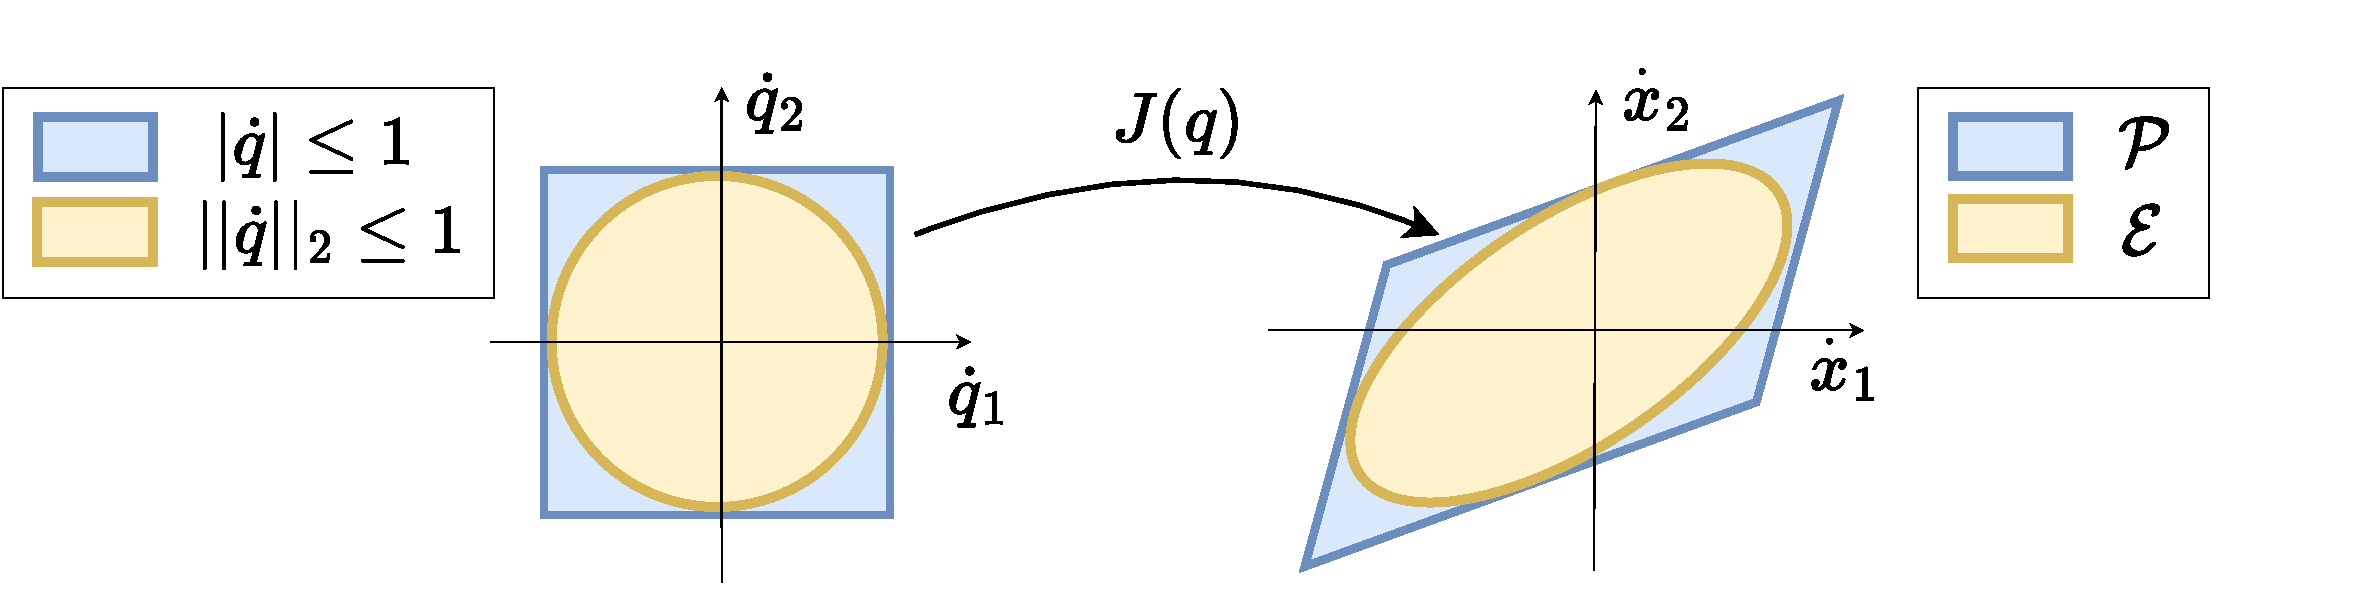
\includegraphics[width=0.7\textwidth]{Chapters/imgs/ellip_poly.pdf}
    \caption{An example manipulability polytope and ellipsoid geometry for a planar $m=2$ robot with $n=2$. The difference between the joint space limits for ellipsoid described with $||\dot{\bm{q}}||_2\leq1$ (orange) and the range limits $\bm{-1}\leq\dot{\bm{q}}\leq\bm{1}$ (blue) is shown on the right. The difference in obtained achievable task space velocity $\dot{\bm{x}}$ polytope $\mathcal{P}$ (blue) and ellipsoid $\mathcal{E}$ (orange) is shown on the right plot. The plots show that both in joint and task space the ellipsoid metric is an underestimation of the true robot's capacity.}
    \label{fig:ellip_poly_dif}
\end{figure}

Once the true robotic actuator limits are considered, the representation of physical abilities becomes convex polytope shaped. As opposed to the manipulability ellipsoid $\mathcal{E}$, manipulability polytope can be defined as
\begin{equation}
    \mathcal{P}(\bm{q}) = \left\{ \dot{\bm{x}} ~|~ \dot{\bm{x}} = J(\bm{q})\dot{\bm{q}},~~ \dot{\bm{q}}_{min}\leq\dot{\bm{q}} \leq \dot{\bm{q}}_{max} \right\}
\end{equation}
The manipulability polytope $\mathcal{P}$ represents an exact solution of the robot's task space velocity capacity, given robot's state $\bm{q}$
and its joint velocity limits $\dot{\bm{q}}$. The difference between the manipulability ellipsoid $\mathcal{E}$ and polytope $\mathcal{P}$ is shown for a simple 2d example on Figure \ref{fig:ellip_poly_dif}.
Polytope based physical ability metrics are the most complete local representation of task space physical abilities of robotic systems and they are used to characterise many task related physical values such as velocities \cite{Lee1997manip, long_constrained_2020}, forces \cite{chiacchio_evaluation_1996}, accelerations \cite{chiacchio_2000}, stiffness \cite{ajoudani2015role}, positioning accuracy \cite{pholsiri2005real}, etc.
The main downside to the polytope based metrics with respect to the ellipsoid based metrics is their computational complexity, making their use somewhat limited to non time critical applications.
% \todos{say that most of the stuff done with other metrics can be done with polytopes as well}

% \todos{
% \begin{itemize}
%     \item for robotics
%     \begin{itemize}
%         \item used to evaluate the robot capacity to execute certain tasks
%         \item to design more capable robots
%         \begin{itemize}
%             \item different visual metrics cable of being used to guarantee stuff
%             \item usually calculated in advance for the whole robot workspace 
%             \item payload for example, or reachable workspace, or wrench closure workspace for parallel robots
%             \item typically not taking in consideration robot's dynamics
%         \end{itemize}
%         \item to exploit robot's full potential when controlling it (or planning its movements)
%         \begin{itemize}
%             \item used in optimisation
%             \item different scalar metrics that are easy to calculate in real time
%             \item manipulability index, and all the other indexes from the overview paper
%             \item also ellipsoids were used for this to find the directions with max movement capacity
%         \end{itemize}        
%     \end{itemize}        
% \end{itemize}
% }

\subsection{Metrics for humans}

Evaluating physical abilities of humans is a much more challenging than for robotic systems, as human bodies are much more complicated systems that depend both on biological and biomechanical, as well as cognitive and psychological factors.

Measuring different physical abilities of human subjects is traditionally done experimentally. The ability of human subjects to achieve different physical quantities such as generate forces \cite{HODDER2016Testing,HOLZBAUR20072442}, reach positions \cite{CASTRO2019108}, execute movements \cite{Jessop2016} or generate stiffnesses \cite{Tsuji1995,Artemiadis2010}, is tested in laboratory environment for a set of predefined human postures or movements. These experiments enable finding precise physical abilities of one or multiple subjects, for the tested motions and postures.  Such experimental analysis are common tools for evaluation of physical abilities in sports \cite{Jessop2016}, where the motions and postures of interest are usually well define, and in rehabilitation \cite{HAISMA2006741} where the aim is to measure the progress of the human subject's recovery. However due to the large variability in human bodies and movements, it is challenging to generalise these results to the human subjects who were not part of the experiments, as well as to different postures and movements, of the same human subjects, that were not tested in the experiments.

In more varied and unstructured settings, where the human postures and movements are harder to characterise, such as in factory setting, the experimental metrics are impractical. For these scenarios, instead of characterising the physical ability of human subject directly, different metrics are developed aiming to evaluate the ergonomics of human postures and movements when executing tasks. These metrics are able to account for variations in human body anthropomorphic structure as well as for different movement and forces generation requirements of the tasks. Such metrics are often defined in a form of standards, such as \textit{Rapid Entire Body Assessment} (REBA) \cite{reba}, \textit{Rapid Upper Limb Assessment} (RULA) \cite{rula} or DULA and DEBA \cite{Yazdani2022} ( their differentiable equivalents), and manuals, such as Great Britain's \textit{Manual Handling Operation Regulations} \cite{health1992manual} or NASA's \textit{Man-systems integration standards} \cite{nasa}. These metrics are designed to give a certain score or a recommendation for the human postures, movements or force generation requirements of the task, in order to evaluate if the task is well suited for human's physical abilities. Common applications of these metrics, in factory settings, have for a goal to evaluate and improve the ergonomics of human's tasks \cite{Busch2017} and workplace layouts\cite{ORE20161, Lietaert2019}. However, these metrics, in order to be task and human subject agnostic, make coarse approximations of human physical abilities which are constraining when it comes to the online human robot collaboration scenarios\cite{maurice2015}. 
%\todo{motivate better, a sentence about problems} 

In order to characterise human's physical abilities, more finely, without the need for time consuming and impractical experimental evaluation, different metrics based on human musculoskeletal models are proposed. Human musculoskeletal models are relatively complete models of human bodies capable of describing different human body's biological and biomechanical parameters as well as its rigid body dynamics. Musculoskeletal models are actuated by muscle-tendon units, capable of applying a range of contracting forces, accelerations and velocities. Similar to robotic systems, several global and local physical ability metrics, based on musculoskeletal models, can be calculated by evaluating how different limits of the muscles as actuators effect human's task related physical abilities, such as to generate forces or motions. 

Several global physical ability metrics based on musculoskeletal models are introduced in literature, such as human upper extremity reachable workspace \cite{Lenarcic1994,Kurillo2013} or comfortable reachable workspace \cite{Figueredo2021}, the comfortablility map of the reachable workspace of human's upper limbs evaluated using RULA and REBA ergonomics scores. In addition to the global metrics many robotics inspired local, state dependent, metrics have been developed as well. Different authors have used their ellipsoid based representations to asses the velocity (manipulability) \cite{Rezzoug2012manipulability}, force \cite{rezzoug_application_2012, lazinica_higher_2010}, acceleration \cite{khatib2009robotics} and stiffness \cite{Artemiadis2010} capacity of humans based on their musculoskeletal models. Several of these ellipsoids have been extend to the more complete polytope representation as well, such as force polytope \cite{sasaki2011vertex, rezzoug_application_2012, carmichael_estimating_2013} and acceleration capacity polytope \cite{khatib2009robotics, demircan2012muscle}. As in the case of robotic systems, polytope based represents the exact solution to the physical ability evaluation, given an appropriate musculoskeletal model. However, as the musculoskeleral models are only an approximation of the true physics of human bodies the accuracy of the calculated physical ability metrics relies entirely on the correspondence between the model and the human subject. Multiple experimental studies were conducted on for the human upper limb force generation capacity, by Rezzoug et al. \cite{biomechanics1010008}, Hernandez et. al \cite{HERNANDEZ2015} as well as Sasaki et al. \cite{lazinica_higher_2010}, where the experimental results were compared to the force capacity polytope and ellipsoid representations. Their results confirm that the polytopes correspond better to the experimentally obtained capacity of the human subjects. However, the results further underline the importance of having an appropriate musculoskeletal model of the human subject. Even though many strategies have been developed for fitting the musculoskeletal models to human subjects in the biomechanics literature mostly based on different forms of scaling \cite{Lund2015, Ziyun2019}, it is still an open field of research. 

With the assumption of an appropriate and well adapted human musculoskeletal model of the human subject, polytopes and ellipsoids present an accurate estimation of the human's task related physical abilities. 
Even though polytopes are more accurate estimation, ellipsoid based representations, due to their computational efficiency, are still a preferred choice when it comes to evaluating human's physical ability, especially in real time applications. The difference in computational complexity between polytope and ellipsoid evaluation for musculoskeletal models is even more exaggerated than for the robotic systems. As the musculoskeletal models often have many muscles (often more than 50) final polytope geometry becomes complex which ultimately has a negative impact of their computation time.

% \todos{
% \begin{itemize}
%     \item for humans
%     \begin{itemize}
%         \item for humans the metrics are mush less exact, mostly empirical
%         \begin{itemize}
%             \item in labs
%             \item per subject
%             \item hard to generalize
%             \item takes time
%         \end{itemize}
%         \item simpler metrics 
%         \item used to evaluate the ergonomics of the human posture, his task or his workspace
%         \begin{itemize}
%             \item evaluated in-situ
%             \item different score based scalar metrics
%             \item ergonomics scores based on different metrics and manuals
%             \item rula, reba, payload manual, nasa and similar
%         \end{itemize}        
%         \item different set of metrics based on human miscalculate models
%         \item based on exact evaluation of different metrics (similar to robots)
%         \begin{itemize}
%             \item used to evaluate maximal human capacities
%             \item more or less all the metrics as for robots can be used
%             \item ellipsoids and polytopes to evaluate the maximal force capacity
%         \end{itemize}   
%         \item there are also those who try to combine the two
%         \item standards + musculoskeletal stuff
%         \begin{itemize}
%             \item comfortability metrics ( a combination of the two ) \cite{Figueredo2021}
%             \item however calculated in advance and relatively complicated to use, no dynamics
%         \end{itemize}   
%     \end{itemize}
    
% \end{itemize}
% }

\subsection{Physical abilities in human-robot collaboration}

Human's and robot's individual physical ability metrics have been used in different human-robot collaboration scenarios. Robot's physical abilities are often calculated in order to make sure that the task requirements comply with the robot's capacity, while human's physical ability and ergonomics metrics are then used to design the suitable robot behavior in order to make the human's task and posture more ergonomic. Such collaboration strategies consider the robot be an action vector with limited resources whose job is to improve the task performance and the human ergonomics at the same time. Examples of such human-centered collaborative scenarios are described by Kim et al. \cite{KIM2021102084}, where the robot adapts the position of the manipulated object in space in order to improve human's ergonomics, or in the context of exoskeleton control by Carmichael et al. \cite{carmichael2013admittance,carmichael_towards_2011} and Pertic et al. \cite{petric2019assistive}, where the robot adapts to different assistance needs of the human operator.

However, when it comes to the human-robot collaboration scenarios where a human and a robot interact physically in order to execute a certain task, characterising their joint physical abilities is still an open research question. Human and robot physical abilities are often expressed in different ways, with different units and with fundamentally different metrics, making the procedure of combining them challenging. Therefore, in order to characterise their joint physical capacity, the first step is to express their individual physical abilities need in the same unified form. 

When it comes to multi-robot physical collaboration, Chiacchio et al. \cite{chiacchio_global_1991} have shown that ellipsoid based metrics can be used to calculate their combined joint velocity (manipulability) capacity. The final joint capacity has an ellipsoid form as well.  However, in their formulation, the collaboration of multiple robots is essentially seen as one larger robot, combining all the joints of all the robots, resulting in the robot with $n=n_1 + n_2 + \ldots$ joints.
\begin{equation}
    \bm{q} = \begin{bmatrix}
        \bm{q}_1\\ \bm{q}_2 \\ \ldots
    \end{bmatrix}, \quad
    \dot{\bm{q}} = \begin{bmatrix}
        \dot{\bm{q}}_1\\\dot{\bm{q}}_2 \\ \ldots
    \end{bmatrix}, \quad
    J(\bm{q}) = \text{diag}([J_1(\bm{q}_1),~ J_2(\bm{q}_2),~\ldots])
\end{equation} 
Where $n_i$ is the number of joints, while $\bm{q}_i$ is the vector of joint positions and $J_i(\bm{q}_i)$ is the jacobian matrix for each one of the robot's involved.

\begin{figure}[!h]
    \centering
    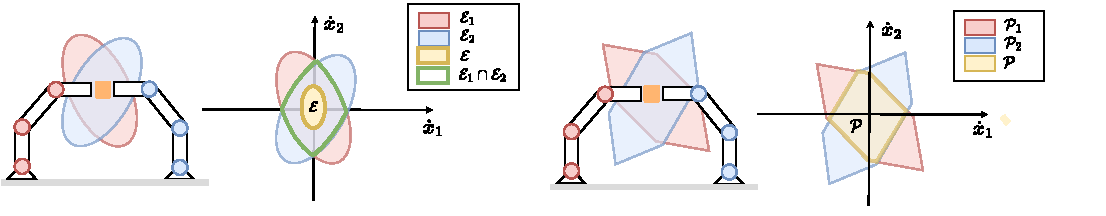
\includegraphics[width=1.05\linewidth]{Chapters/imgs/collab_manip_poly.pdf}
    \caption{Comparison of using ellipsoids (left) and polytopes (right) for collaborative physical ability calculation. Using polytopes, the common velocity capacity of the two robots is calculated as the intersection of their polytopes $\mathcal{P}=\mathcal{P}_1 \cap \mathcal{P}_2$. In ellipsoid case the intersection of the ellipsoids (green) is no longer an ellipsoid and it is hard to characterise, while the collaborative ellipsoid $\mathcal{E}$ (orange) introduced by Chiachio et al. \cite{chiacchio_global_1991} is a large underestimation of the true joint capacity.}
    \label{fig:collab_mani_poly}
\end{figure}
With such large number of joints, the euclidean norm $||.||_2$ limits present a large under-approximation of the real robot's limits, resulting in large under-approximation of the true capacity of the collaboration. As shown on the example on Figure \ref{fig:collab_mani_poly}, a more precise approach would be to intersect the ellipsoids calculated independently for all the robots $$\mathcal{E}=\mathcal{E}_1 \cap \mathcal{E}_2  \cap \ldots$$ However, the intersection operation over ellipsoids is hard to characterise and to evaluate, as the intersection of two ellipsoid is no longer an ellipsoid, and even if the intersection of the ellipsoids is obtained, it is just an approximation of true common capacity. 

Expressing the robot's physical ability in the polytope form however is not just the exact solution, but enables using the polytope algebra to do different operations, such as sum, intersection and convex-hull. These operations are well defined and can be calculated efficiently. The work from Jihong Lee \cite{lee2001velocity} shows that polytopes metrics can be used to describe the common velocity capacity of multi-arm collaborative robotic system.  The work describes an efficient way of calculating the joint velocity capacity by intersecting the individual polytopes of each one of the robots involved, resulting in a convex polytope shaped joint velocity capacity $$\mathcal{P}=\mathcal{P}_1 \cap \mathcal{P}_2  \cap \ldots$$
By exploiting different polytope algebra operations it is possible to express different physical collaboration scenarios as well. For example, if now the robots would be re-arranged from the parallel to the serial configuration, where the robot would be stacked one on top of the other, their joint velocity capacity would correspond to the Minkowski sum of their individual capacity $$\mathcal{P}=\mathcal{P}_1 \oplus \mathcal{P}_2  \oplus \ldots$$

\begin{figure}[!h]
    \centering
    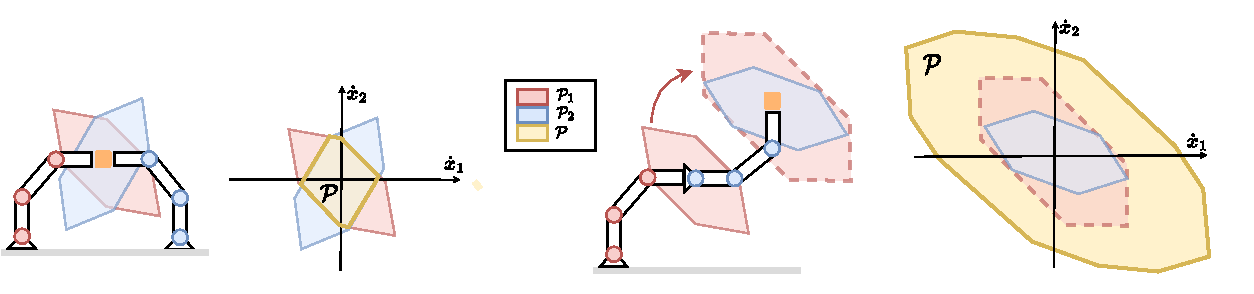
\includegraphics[width=\linewidth]{Chapters/imgs/collab_serial_parallel.pdf}
    \caption{Two examples of using polytope based metrics for joint achievable velocity capacity calculation of multiple robots collaborating. Figure on the left shows the parallel collaboration where the common capacity is calculated with the intersection. Figure on the right shows the serial collaboration where the common capacity is a Minkowski sum of their individual capacity. As the capacity is calculated at the end-effector of the second robot, the velocity polytope $\mathcal{P}_1$ of the first robot has to be transformed the same position (in red dashed border).}
    \label{fig:collab_serial_parallel}
\end{figure}
Figure \ref{fig:collab_serial_parallel} shows a simplified plannar example of the joint velocity capacity calculation for parallel and serial robot arrangement.

In summary, the polytope representation enables the physical abilities of robots, humans, and their collaboration to be expressed through a unified format. Furthermore, as many different physical abilities of humans and robots can be expressed in polytope form, it has the potential to provide an important set of tools for evaluating different collaboration tasks.
For example, by evaluating different physical abilities relevant to the task, it enables characterising if the task is more suitable for humans, robots or for different modes of their physical collaboration.  


% \todos{
% \begin{itemize}
%     \item what about collaboration metrics
%     \item Some metrics have been used but still very limited
%     \item when it comes to characterising their common capacity
%     \begin{itemize}
%         \item payload metrics might be used - very limiting
%         \item and ellipsoid based stuff from chiacchio - robots
%         \item lee also with polytopes a bit - robots
%         \item we still lack proper metrics to unify the humans and robots
%         \item they are usually expressed in different ways and hard to combine
%     \end{itemize}
%     \item Different ways of enhancing collaboration using physical ability metrics
%     \begin{itemize}
%         \item Collaborative workspace design for example - vincent paper
%         \item visualisation to the user 
%         \item Communicate the current robot state to the operator when collaborating
%         \item assist as needed control of exoskeletons also maybe (ellipsoids petric + polytopes carmichael)
%         \item but still not considering robot's capacity - robot only adapts to the human needs
%     \end{itemize}
% \end{itemize}
% }


\subsection{Why polytopes?}

As described in the previous sections, polytope representation of physical abilities accurately 
characterises the physical abilities of robotic manipulators, at the same time being the most complete approximation of human physical abilities based on musculoskeletal models. Additionally, since most of the well known polytope formulations for robotic systems can be formulated as polytopes for musculoskeletal models as well, they enable evaluating and comparing human's and robot's physical abilities in a unified manner. Furthermore, the polytope algebra enables operations over multiple polytopes and, in that way, has a potential to enable characterising common physical abilities of humans and robots involved in different physical collaboration scenarios. 

When it comes to using polytopes in practical applications, there are two standard ways of representing them: as a set of vertices (vertex representation) or as a set of inequality constraints corresponding to its faces (half-plane representation) \cite{fukuda2004frequently}. Transforming a polytope into these standard representations enables using different efficient tools from computational geometry and polytope algebra in order to do operations over polytopes, for example find minimal distance between polytopes \cite{Ong1997gjk}, polytope volume \cite{Lawrence1991Volume} or calculate the convex hulls \cite{Barber1996}, Minkowski sums \cite{BARKI2009525}, intersections and unions of multiple polytopes \cite{Tiwary2008}. Additionally, it opens doors for different simplification strategies of polytopes, by finding the inner and outer approximations of polytopes using spheres \cite{Botkin1994} or cubes \cite{BEMPORAD2004151}.

Furthermore, as discussed by Finotello et al. \cite{Finotello1998}, polytopes enable calculating many other local different performance metrics, such as Maximum Available Value (MAV) corresponding to the highest achievable magnitude of the task space variable (velocity, acceleration, force, static error, etc.), Maximal Isotropic Value (MIV) corresponding to the maximal value achievable in all the directions in space or Directional Index (DI) \cite{boschetti_minto_2023} corresponding to the maximum achievable task space variable in certain direction in space or calculating. Additionally, polytope volume and major (preferred) axis can be used as performance metrics as well \cite{chiacchio_global_1991, Long2018Evaluating}.

In case of characterising physical abilities, transforming the polytopes to the vertex representation enables using efficient triangulation algorithms from computational geometry. Most of the standard visualisation tools can visualise such triangulated meshes in very efficient manner, even in real time. 
In the context of human-robot collaboration, an example application of polytope visualisation was proposed by Zolotas et al. \cite{Zolotas2021}, where the robot's velocity polytopes were used to inform the operator about the robot's movement capacity during the teleportation task. Similar application was recently proposed by Weistroffer et al. \cite{Weistroffer2022Using}, where the polytopes of robot's force capacity were visualised to the operator designing the collaborative workspace with the aim to improve its safety and ergonomics. 

Polytopes can be expressed as a set of linear inequalities $A\bm{x}\leq\bm{b}$, that can be integrated into different optimisation problems in a form of linear inequality constraints. Most of the standard Quadratic Programming (QP) \cite{boggs_tolle_1995} and Linear Programming (LP) \cite{GOLDFARB198973} solvers support the inequality constraints in an efficient manner. A typical example applications often based on different optimisation strategies are robot control and trajectory planning applications. In the context of human-robot collaboration, being able to consider both robot's and human's physical abilities with in those contexts, opens doors for creating more human-centred robot control (or trajectory planning) strategies where robot's behaviour is adapted (planned), not just with respect to its own physical abilities, but also to the ones of the human.
Potential benefits of considering human's physical abilities for creating human-centred robot control were demonstrated in the context of assistive exoskeletons. In these scenarios, the robot provides the assistance to the operator adapted to his current physical ability, so called \textit{Assist As Needed} (AAN)\cite{carmichael2013admittance} control paradigm.
However, as the polytope representation of human physical abilities based on musculoskeletal models results in a highly complex computational problem to solve, in order to be used in real-time applications, so far all solutions proposed in the literature use different approximations of human's physical abilities. In the work by Carmichael et al. \cite{carmichael_towards_2011}, a coarse approximation of human's force capacity was used, Aldini et al.\cite{Aldini2021RealTime} have used a learning based approach to estimate human's force ability using polynomial fitting, while in the work by Petric et al.\cite{petric2019assistive}, similar strategy was used where human's force abilities were approximated using ellipsoids.

Therefore, polytope representation provides an accurate representation of both humans' and robots' physical abilities in a unified manner. Additionally, it enables characterising the common physical abilities of humans and robots interacting physically when executing certain task as well. Representing these capacities in the polytope form enables using many efficient tools form the polytope algebra and computational geometry to perform operations over polytopes and to extract useful information concerning the tasl, for example different performance indicators. Additionally, polytopes can be transformed to more standard forms such as a set of vertices or set of inequalities which can then be used with standard visualisation tools and integrated in different optimisation problems, opening many doors in human-robot collaborative applications.

This chapter further brings an overview of common polytope formulations for characterising different physical abilities of robots in section \ref{ch:robot_metrics} and humans in section \ref{ch:human_metrics}. Section \ref{ch:collab_metrics} then discusses combining their individual polytopes using polytope algebra, in order to characterise their common physical abilities when interacting physically in the context of the object manipulation. Finally, section \ref{ch:collab_metrics_overview} brings the structured view on the introduced polytope formulations and their use in characterising the human-robot interaction abilities.


% \todos{
% \begin{itemize}
%     \item polytope based metrics might be able to close the gap
%     \item in our opinion the best ones - unifying most of the other metrics
%     \item exact solution 
%     \item encapsulate many of the other metrics inside (volume, direction of maximal magnitude, singularity, ....)
%     \item can be easily visualised
%     \item defined both for robots and humans (based on musculoskeletal models)
%     \item can be used in optimisation
%     \item operation over polytopes (sum, intersection convex-hull) well defined as opposed to the other metrics
% \end{itemize}
% }
\section{Polytope representation of physical abilities}
\label{ch:poly_metrics}
Physical ability characterisations based on polytopes are numerous in the literature, therefore the aim of this section is to provide an overview of common polytope formulations for different physical abilities of robotic systems and humans, based on their musculoskeletal models. Additionally, section \ref{ch:collab_metrics} demonstrates the use of polytopes to calculate the physical abilities in collaborative scenarios. Finally, section \ref{ch:which_metric_which} brings the categorisation of the common polytope formulations with respect to the nature of their formulation.

\subsection{Robotic manipulators}
\label{ch:robot_metrics}

Physical ability characterisations based on polytopes are most accurate local, state dependent, metrics for the performance analysis of robotic systems \cite{pholsiri2005real,Finotello1998}. They describe a mapping between the robot's actuator limits (torques, accelerations , velocities, etc.) and the limits of different task space variables (wrenches, accelerations, velocities, etc.) . 

The aim of this section is to provide an overview of common polytope formulations for robotic systems in an unified view.  Therefore, section \ref{ch:robot_dyn_kin} beings a quick overview of the dynamics and kinematics equations for robotic systems, used for different polytope definitions. Definitions 
of common polytope characterisations of physical abilities are then described in subsequent chapters.

\subsubsection{Dynamics and kinematics relationships}
\label{ch:robot_dyn_kin}
The actuation limits, of a robotic manipulator with $n$ joints, are commonly specified as independent ranges of achievable actuator positions $\bm{q}\in \mathbb{R}^n$, velocities $\dot{\bm{q}}\in \mathbb{R}^n$, actuator torques $\bm{\tau}\in \mathbb{R}^n$ and sometimes even torque derivative $\dot{\bm{\tau}}\in \mathbb{R}^n$.
\begin{subequations}
\begin{align}
\bm{q} &\in [ {\bm{q}}_{min}, {\bm{q}}_{max}], \quad\dot{\bm{q}} \in [\dot{\bm{q}}_{min},  \dot{\bm{q}}_{max}], \\
\quad\bm{\tau} &\in [\bm{\tau}_{min},  \bm{\tau}_{max}],
\quad\dot{\bm{\tau}} \in [\dot{\bm{\tau}}_{min},  \dot{\bm{\tau}}_{max}] \label{eq:dyn_limits:torque}
\end{align}
\label{eq:dyn_limits}
\end{subequations}
The dynamical model, of a standard serial robotic manipulator with a fixed base, is commonly defined as
\begin{equation}
M(\bm{q})\ddot{\bm{q}} + C(\bm{q},\dot{\bm{q}})\dot{\bm{q}} + \bm{g}(\bm{q}) + J^T(\bm{q})\bm{f} = \bm{\tau} 
\label{eq:dyn_model_rob}
\end{equation}
where $M(\bm{q}) \in \mathbb{R}^{n \times n}$ and $C(\bm{q},\dot{\bm{q}})\in \mathbb{R}^{n \times n}$ are its inertia and Coriolis matrices, $\bm{g} (\bm{q})\in \mathbb{R}^n$ is the state dependent gravity vector, $J(\bm{q}) \in \mathbb{R}^{m\times n}$ is the state dependant jacobian matrix, $\bm{f}\in \mathbb{R}^m $ is the vector of applied external wrenches and $\bm{q},\dot{\bm{q}},\ddot{\bm{q}}$ are robot's joint positions, velocities and accelerations respectively.

Furthermore, the mapping between the $n$ dimensional space of robot's actuator (joint) positions $\bm{q}\in \mathbb{R}^n$ and the $m$ dimensional task space positions $\bm{x} \in \mathbb{R}^m$ can be found through the robot's forward kinematics 
\begin{equation}
    \bm{x} = f_{fk} (\bm{q})
\end{equation}
whereas the task space velocity $\dot{\bm{x}}\in \mathbb{R}^m$, acceleration $\ddot{\bm{x}}\in \mathbb{R}^m$ and jerk $\dddot{\bm{x}}\in \mathbb{R}^m$ can be found through the state dependent  $\{\bm{q},\dot{\bm{q}},\ddot{\bm{q}}\}$  and nonlinear mapping
\begin{subequations}
\begin{align}
\dot{\bm{x}}&= {J}(\bm{q})\dot{\bm{q}} \label{eq:js_to_cs_vaj:vel}\\
\ddot{\bm{x}}&= J(\bm{q})\ddot{\bm{q}} + \dot{J}(\bm{q},\dot{\bm{q}})\dot{\bm{q}} \label{eq:js_to_cs_vaj:accel}\\
\dddot{\bm{x}}&= J(\bm{q})\dddot{\bm{q}} + 2\dot{J}(\bm{q},\dot{\bm{q}})\ddot{\bm{q}} + \ddot{J}(\bm{q},\dot{\bm{q}},\ddot{\bm{q}})\dot{\bm{q}}\label{eq:js_to_cs_vaj:jerk}
 \end{align} \label{eq:js_to_cs_vaj}
\end{subequations}
were $J(\bm{q}) $ is the jacobian matrix
\begin{equation}
    J(\bm{q}) = \frac{\partial f_{fk} (\bm{q})}{\partial \bm{q}}
\end{equation}
while $\dot{J}(\bm{q},\dot{\bm{q}})$ and $\ddot{J}(\bm{q},\dot{\bm{q}},\ddot{\bm{q}})$ are its first and second time derivatives.


It is worth noting that in general case, $m$ dimensional task space might include positions and orientations, for example if the task space corresponds to the Cartesian space, where $m=6$. When the task space includes orientations, the task space pose (including the position and orientation) is often expressed is the homogeneous matrix form $\bm{x}\in SE(3)$. Then the task space velocity vector $\dot{\bm{x}}\in\mathbb{R}^6$ becomes the Cartesian space \textit{twist vector} $\bm{\nu}$, expressing the translation and rotation velocity at the same time. However, in such cases, the twist $\bm{\nu}$ does no longer correspond to the time derivative of the task space pose $\bm{\nu}\neq\frac{d\bm{x}}{dt}$. Despite this distinction, for simplicity reasons, this work uses the notation $\dot{\bm{x}}$, $\ddot{\bm{x}}$, and $\dddot{\bm{x}}$ to represent velocity, acceleration, and jerk of the task space variables, respectively.

When considering certain fixed robot state $\{\bm{q},\dot{\bm{q}},\ddot{\bm{q}}\}$, robot's dynamical model (\ref{eq:dyn_model_rob}) and the joint to task space mapping (\ref{eq:js_to_cs_vaj}) become linear, as the state dependent matrices become fixed. Using these linear and affine mappings the achievable sets of different task space variables (ex. velocity $\dot{\bm{x}}$, accelerations $\ddot{\bm{x}}$ or wrenches $\bm{f}$), given the range of robot's actuator limits (\ref{eq:dyn_limits}), can be found through the equations (\ref{eq:dyn_model_rob}) and (\ref{eq:js_to_cs_vaj}). The obtained achievable sets then have a form of convex polytopes as the mapping between the robot limits and the task space variables is linear.


\paragraph*{Kinematic joint limits} As a precise robot's dynamical model is sometimes hard to obtain, instead of specifying the actuator torque limits (\ref{eq:dyn_limits:torque}), the manufacturers often rather specify robot's actuator limits in a kinematic form, considering them to have limited and constant acceleration $\ddot{\bm{q}} \in \mathbb{R}^n$ and jerk $\dddot{\bm{q}} \in \mathbb{R}^n$ limits.
\begin{equation}
\ddot{\bm{q}} \in [\ddot{\bm{q}}_{min}, \ddot{\bm{q}}_{max}], ~~ \dddot{\bm{q}} \in [ \dddot{\bm{q}}_{min}, \dddot{\bm{q}}_{max}] 
\label{eq:kin_limits}
\end{equation}
Using these kinematic actuator limits, the linearisation procedure of the mapping (\ref{eq:js_to_cs_vaj}) around given robot state $\{\bm{q},\dot{\bm{q}},\ddot{\bm{q}}\}$, can then be used to obtain the polytope shaped achievable sets of kinematic task space variables (ex. velocity $\dot{\bm{x}}$, acceleration $\ddot{\bm{x}}$, jerk $\dddot{\bm{x}}$).



\paragraph*{} Many well known polytope formulations for characterising the physical abilities of robotic manipulators are proposed in the literature, characterising the influence of robots dynamics (\ref{eq:dyn_limits}) and kinematics joint limits (\ref{eq:kin_limits}) on the task space variables through its linearised dynamics (\ref{eq:dyn_model_rob}) and kinematics (\ref{eq:js_to_cs_vaj}) equations. Some of the most common polytope formulations are listed in the following sections.

\subsubsection{Velocity polytope}
\label{ch:vel_poly}

Achievable task space velocity capacity is a common physical ability metric for robotic manipulators describing its ability to generate task space velocities $\dot{\bm{x}}$ in different directions in space, given its joins space velocity $\dot{\bm{q}}$ limits. Robot's velocity capacity is commonly know as its manipulability or dexterity capacity as well. This metric has been first introduced by Yoshikawa \cite{yoshikawa_manipulability_1985} in the ellipsoid form and later extended to the polytope form \cite{chiacchio_global_1991, Lee1997manip}. %\todo{try finding the paper: 
%"Kinetostatic performance limits of cooperating robot manipulators using force-velocity polytopes"
%}

For any fixed robot configuration $\bm{q}$ the ranges of joint velocity limits 
\begin{equation}
   \dot{\bm{q}}\in\left[\dot{\bm{q}}_{min}, \dot{\bm{q}}_{max} \right]
\end{equation}
can be projected to the $m$ dimensional task space using the jacobian matrix $J(\bm{q})$, obtaining the convex polytope of achievable task space velocities  
\begin{equation}
    \mathcal{P}_v(\bm{q}) = \left\{ \dot{\bm{x}} \in \mathbb{R}^m ~|~ \dot{\bm{q}}\in\left[\dot{\bm{q}}_{min}, \dot{\bm{q}}_{max} \right], ~~ \dot{\bm{x}} = J(\bm{q})\dot{\bm{q}} \right\}
    \label{eq:poly_vel_rob}
\end{equation}

Velocity capacity metrics are important tools for evaluating robot's movement capacity in different directions in space for a given configuration $\bm{q}$, while the polytope form is their exact representation. Different variants of polytope formulations are commonly used for robot redundancy resolution, by finding the robot configurations that maximise the robot's movement capacity and avoid singular positions\cite{Marani2002,Thygeson2017}, which can be seen as a zero velocity capacity in certain directions in space \cite{merlet_jacobian_2006}.  They have also been used for path planning \cite{Pardi2020,Nagatani2002} and object grasping \cite{Fei2019,XU2021300}. 

The polytope representation though is less commonly used in time-critical applications, due to their computational complexity. However, Long et al. have shown that polytopes can be used for whole body humanoid robot control \cite{long_constrained_2020} in real-time. Recently, Zolotas et al. have shown their potential to be used for real-time visualisation to the user in the case of robot teleportation \cite{Zolotas2021}. 

\subsubsection{Kinematic Acceleration and Jerk polytope}\label{ch:kin_accel_jerk}
In a similar manner to the achievable velocity polytope $\mathcal{P}_v$, the achievable task space acceleration $\ddot{\bm{x}}$ and jerk $\dddot{\bm{x}}$ sets can be expressed using the kinematic mapping (\ref{eq:js_to_cs_vaj}). 

Given the limits of the actuator accelerations $\ddot{\bm{q}}$ and a given robot state $\{\bm{q},\dot{\bm{q}}\}$, the achievable polytope $\mathcal{P}_a$ of task space accelerations $\ddot{\bm{x}}$ can be found using the mapping (\ref{eq:js_to_cs_vaj:accel}).
\begin{equation}
    \mathcal{P}_a(\bm{q}, \dot{\bm{q}}) = \left\{ \ddot{\bm{x}} \in \mathbb{R}^m ~|~ \ddot{\bm{q}}\in\left[\ddot{\bm{q}}_{min}, \ddot{\bm{q}}_{max} \right], ~~ \ddot{\bm{x}} = J(\bm{q})\ddot{\bm{q}} + \bm{a}_b(\bm{q}, \dot{\bm{q}})  \right\}
    \label{eq:poly_accel_kin}
\end{equation}
where $\bm{a}_b(\bm{q}, \dot{\bm{q}})$ is considered as a constant bias term for any given robot state $\{\bm{q},\dot{\bm{q}}\}$
\begin{equation}
    \bm{a}_b(\bm{q}, \dot{\bm{q}}) = \dot{J}(\bm{q},\dot{\bm{q}})\dot{\bm{q}}
\end{equation}.

The achievable task space jerk polytope $\mathcal{P}_j$ can be found for any given robot state $\{\bm{q},\dot{\bm{q}},\ddot{\bm{q}}\}$, by considering a limited range of actuator jerks $\dddot{\bm{q}}$ and using the mapping (\ref{eq:js_to_cs_vaj:jerk})
\begin{equation}
    \mathcal{P}_j(\bm{q}, \dot{\bm{q}}, \ddot{\bm{q}}) = \left\{ \dddot{\bm{x}} \in \mathbb{R}^m ~|~ \dddot{\bm{q}}\in\left[\dddot{\bm{q}}_{min}, \dddot{\bm{q}}_{max} \right], ~~ \dddot{\bm{x}} = J(\bm{q})\dddot{\bm{q}} + \bm{j}_b(\bm{q}, \dot{\bm{q}},\ddot{\bm{q}}) \right\}
    \label{eq:poly_jerk_kin}
\end{equation}
where $\bm{j}_b(\bm{q}, \dot{\bm{q}},\ddot{\bm{q}})$ is a constant bias term for any fixed robot state $\{\bm{q},\dot{\bm{q}},\ddot{\bm{q}}\}$
\begin{equation}
    \bm{j}_b(\bm{q}, \dot{\bm{q}},\ddot{\bm{q}}) =2\dot{J}(\bm{q},\dot{\bm{q}})\ddot{\bm{q}}+ \ddot{J}(\bm{q},\dot{\bm{q}},\ddot{\bm{q}})\dot{\bm{q}}
\end{equation}

An example application of the jerk and acceleration polytopes is described by Grandguillaume et al. where the polytopes are used to find the optimal tool orientation for 5-axis milling \cite{Grandguillaume2021}.

\subsubsection{Precision (maximal positioning error) polytope }

Robotic manipulators often have limited positioning precision of their actuators. Actuator precision depends on many different factors, such as position sensor used, motor gearing, motion control strategy etc \cite{pholsiri2005real,Finotello1998}. However, in most cases the manufacturers are able to provide the limits on the maximal positioning error for each of the actuators within a certain range
\begin{equation}
    \delta\bm{q} \in [\delta\bm{q}_{min}, \delta\bm{q}_{min}]
    \label{eq:pos_error}
\end{equation}

Depending on the robot's configuration $\bm{q}$ the actuator position error $\delta\bm{q}$ will produce different task space positioning errors, their relationship can be calculated through the kinematic mapping (\ref{eq:js_to_cs_vaj:vel})
\begin{equation}
    \delta\bm{x} = J(\bm{q})\delta \bm{q}
\end{equation}
where $\delta\bm{x}\in\mathbb{R}^m$, in general case presents both position and orientation error.

The limits of the task space positioning error $\delta \bm{x}$ in a certain robot configuration $\bm{q}$, given the limits (\ref{eq:pos_error}) specified by the manufacturer, can be expressed by a convex polytope $\mathcal{P}_\delta$
\begin{equation}
    \mathcal{P}_\delta(\bm{q}) = \left\{ \delta \bm{x} \in \mathbb{R}^m ~|~ \delta  {\bm{q}}\in\left[ \delta {\bm{q}}_{min}, \delta {\bm{q}}_{max} \right], ~~  \delta  {\bm{x}} = J(\bm{q}) \delta {\bm{q}} \right\}
    \label{eq:poly_precision_rob}
\end{equation}

\subsubsection{Wrench/Force polytope}
\label{ch:poly_force}
Task space force (or more generally wrench) capacity metric is one of the most well known physical capacity metrics for robotics manipulators alongside the velocity (manipulability) capacity. It has been first introduced by Chiacchio et al. \cite{chiacchio_evaluation_1996} in a form of an ellipsoid as well as in the polytope form.

This metric establishes the relationship between the robot's actuator torque limits $\bm{\tau}$ and the achievable set of the task space wrenches $\bm{f}$.
Given the robot's manipulators dynamics equation (\ref{eq:dyn_model_rob}) 
\begin{equation}
\underbrace{M(\bm{q})\ddot{\bm{q}} + C(\bm{q},\dot{\bm{q}})\dot{\bm{q}} + \bm{g}(\bm{q})}_{\bm{\tau}_b(\bm{q},\dot{\bm{q}},\ddot{\bm{q}})} + J^T(\bm{q})\bm{f} = \bm{\tau} 
\end{equation}
for any given robot state $\{\bm{q},\dot{\bm{q}}\}$, and given joint acceleration $\ddot{\bm{q}}$ to be achieved, the effects of the robot's motion and the gravity can be expressed as a constant torque vector $\bm{\tau}_b(\bm{q},\dot{\bm{q}},\ddot{\bm{q}})$. Then the polytope of achievable task space wrenches $\bm{f}$ can be expressed as
\begin{equation}
    \mathcal{P}_f(\bm{q},\dot{\bm{q}},\ddot{\bm{q}}) = \left\{ \bm{f} \in \mathbb{R}^m ~|~ \bm{\tau}\in\left[\bm{\tau}_{min}, \bm{\tau}_{max} \right], ~~ J^T(\bm{q})\bm{f} = \bm{\tau} -\bm{\tau}_b(\bm{q},\dot{\bm{q}},\ddot{\bm{q}}) \right\}
    \label{eq:poly_force_rob}
\end{equation}

If achievable wrench capacity $\mathcal{P}_f$ is evaluated in kinetostatic conditions $\dot{\bm{q}},\ddot{\bm{q}}\approx\bm{0}$, the torque bias vector $\bm{\tau}_b$ corresponds to the gravity vector $\bm{g}(\bm{q})$ 
\begin{equation}
    \bm{\tau}_b(\bm{q},\bm{0},\bm{0}) = \bm{g}(\bm{q})
\end{equation}

As wrench polytopes describe the feasible range of task space wrenches that the robot can apply in certain configuration, they can be used in many different analysis applications as a performance metric, as well as in robot control in order to guarantee that the task requirements are within robot's capacity. An example application of wrench capacity polytopes for performance analysis of robotic excavator is described by Zou et al. for \cite{Zou2019}. Ferrolho et al. \cite{ferrolho_residual_2020} have described the application of wrench polytopes in offline dynamic trajectory planning. On the other hand, the applications of wrench polytopes in real-time applications are less common, mostly due to their computational complexity. However, Orsolino et al. \cite{Orsolino2018} have recently showed the application of wrench polytopes in real-time control of legged robots.

\subsubsection{Acceleration polytope}
\label{ch:accel_poly_robot}

The kinematic acceleration capacity described in section \ref{ch:kin_accel_jerk} considers constant and independent acceleration capacity for each robot's actuator (\ref{eq:kin_limits}), however the true acceleration limits of the robot's actuators depend on their torque capacity (\ref{eq:dyn_limits}) as well as on the robot's inertia 
$M(\bm{q})$ which is highly configuration dependent. 

Given the robot's dynamics equations (\ref{eq:dyn_model_rob}) 
\begin{equation}
M(\bm{q})\ddot{\bm{q}} + \underbrace{C(\bm{q},\dot{\bm{q}})\dot{\bm{q}} + \bm{g}(\bm{q}) + J^T(\bm{q})\bm{f}}_{\bm{\tau}_b(\bm{q},\dot{\bm{q}},\bm{f}) } = \bm{\tau} 
\end{equation}
for any given robot state $\{\bm{q},\dot{\bm{q}}\}$ and applied external wrench $\bm{f}$, the effects of the robot's motion, the gravity as well as the applied external wrenches, can be grouped in a constant torque vector $\bm{\tau}_b(\bm{q},\dot{\bm{q}},\bm{f})$. Then the actuator acceleration $\bm{q}$ can be expressed in relationship to the applied joint torque $\bm{\tau}$
\begin{equation}
    \ddot{\bm{q}} = M(\bm{q})^{-1}\bm{\tau} - M(\bm{q})^{-1}\bm{\tau}_b(\bm{q},\dot{\bm{q}},\bm{f})
\end{equation}
Finally, the actuator accelerations $\ddot{\bm{q}}$ can be transformed to the task space using the mapping (\ref{eq:js_to_cs_vaj:accel})
\begin{equation}
    \ddot{\bm{x}} = J(\bm{q})M(\bm{q})^{-1}\bm{\tau} - \underbrace{J(\bm{q})M(\bm{q})^{-1}\bm{\tau}_b(\bm{q},\dot{\bm{q}},\bm{f}) + \dot{J}(\bm{q}, \dot{\bm{q}})\dot{\bm{q}}}_{\bm{a}_b(\bm{q},\dot{\bm{q}},\bm{f})}
\end{equation}
where $\bm{a}_b(\bm{q},\dot{\bm{q}},\bm{f})$ presents a constant bias vector for any fixed joint state $\{\bm{q},\dot{\bm{q}},\bm{f}\}$. The polytope $\mathcal{P}_a$ of achievable task space accelerations $\ddot{\bm{x}}$ can then be expressed as
\begin{equation}
    \mathcal{P}_a(\bm{q},\dot{\bm{q}},\bm{f}) = \left\{ \ddot{\bm{x}} \in \mathbb{R}^m ~|~ \bm{\tau}\in\left[\bm{\tau}_{min}, \bm{\tau}_{max} \right], ~ \ddot{\bm{x}} = J(\bm{q})M(\bm{q})^{-1}\bm{\tau} - \bm{a}_b(\bm{q},\dot{\bm{q}},\bm{f}) \right\}
    \label{eq:pol_accleration_rob}
\end{equation}

As opposed to the kinematic acceleration polytope (\ref{eq:poly_accel_kin}) described in section \ref{ch:kin_accel_jerk}, this formulation not only represents more realistic acceleration capacity but it is able to account for the effect of the robot's motion, the effects of the gravity as well as its potential payload etc. 

This metric has been initially introduced by Chiacchio \cite{chiacchio_2000} in the ellipsoid form and later extended to the polytope form by  Rosenstein and Grupen \cite{rosenstein2002velocity}. An application of this metric in off-line analysis has been proposed by Jang and Lee \cite{Jang2009}, using the acceleration polytopes to analyse and optimise multi-fingered object grasping. Acceleration polytopes are used in real-time robot control applications as well. For example, Jeong and Tsagarakis \cite{jeong2006optimal} proposed an application of acceleration polytopes for robotic manipulators in order to optimise the robot's braking characteristics in real-time and to reduce the impact forces. 

\subsubsection{Stiffness polytope}
\label{ch:robot_stiffness_poly}
A different well known task space physical ability metrics for robotic manipulators is related to impedance control. If a certain frame of the robotic manipulator (ex end-effector frame) is controlled to have a behaviour of virtual spring with the task space stiffness $K_c \in \mathbb{R}^{m\times m}$
\begin{equation}
    \bm{f} = K_c \Delta\bm{x}
\end{equation}
where $\bm{f}\in\mathbb{R}^m$ is the  external wrench applied to the robot (by the environment or a human operator), and the $\Delta \bm{x}\in\mathbb{R}^m$ is the resulting displacement corresponding to the virtual spring with the square, $m\times m$, stiffness matrix $K_c$, where $m$ is the task space dimension.  In case of standard impedance control for a robotic manipulator in Cartesian space, controlling both position and orientation ($m=6$), the displacement vector $\Delta \bm{x}$ contains both translation and orientation displacements produced by the wrench $\bm{f}$.
Given a certain range of external wrenches that are expected to be applied by the environment (or the human operator) 
\begin{equation}
    \bm{f}\in\left[\bm{f}_{min}, \bm{f}_{max} \right]
    \label{eq:force_stiff_range}
\end{equation}
the maximal task space displacement $\Delta \bm{x}$ (position and orientation) can be expressed as a convex polytope 
\begin{equation}
    \mathcal{P}_\Delta = \left\{ \Delta\bm{x} \in \mathbb{R}^m ~|~ \bm{f}\in\left[\bm{f}_{min}, \bm{f}_{max} \right], ~~ K_c\Delta\bm{x} = \bm{f} \right\}
\end{equation}

If the stiffness control is done in joint space, where the $n$ robot's actuators are controlled in a way to produce a virtual spring behavior with a stiffness $K_j\in \mathbb{R}^{n\times n}$
\begin{equation}
    \bm{\tau} = K_j \Delta\bm{q}
\end{equation}
This joint space stiffness matrix $K_j$ can be used to find the robot state dependent task space stiffness $K_c$ \cite{Salisbury1980}
\begin{equation}
     K_c(\bm{q})^{-1} = J(\bm{q}) K_j^{-1}J(\bm{q})^T
     \label{eq:stiffness_roobt_eef}
\end{equation}
The matrix $K_j$ is a square $n \times n$ matrix, which is in most cases diagonal and has a full rank, while the jacobian matrix is $m\times n$ shaped and configuration dependent. If the jacobian matrix $J(\bm{q})$ is approaching to its singularity, as the singularity can be seen as a reduction of the task space dimension $m$, the resulting robotic manipulator's stiffness would be approaching infinity in that direction. 
%In singular case however, the task space stiffness matrix $K_c(\bm{q})$ cannot be obtained by simply inverting the equation (\ref{eq:stiffness_roobt_eef}). 

Given the same range of expected external wrenches (\ref{eq:force_stiff_range}), the polytope of maximal task space displacements $\Delta\bm{x}$ can then be expressed as
\begin{equation}
    \mathcal{P}_\Delta(\bm{q}) = \left\{ \Delta\bm{x} \in \mathbb{R}^m ~|~ \bm{f}\in\left[\bm{f}_{min}, \bm{f}_{max} \right], ~~ K_c(\bm{q})\Delta\bm{x} = \bm{f} \right\}
\end{equation}


Neither of these formulations takes in consideration the robot's wrench capacity though, they both consider that the robot is capable of generating all the wrenches in the expected range (\ref{eq:force_stiff_range}). 
In order to make sure that the robot's wrench capacity is not exceeded when calculating the maximal task space displacement polytope $\mathcal{P}_\Delta$ (both for joint space and task space stiffness control) the external wrench range (\ref{eq:force_stiff_range}) needs to be intersected with the robot's  wrench polytope  $\mathcal{P}_f$ described in the section \ref{ch:poly_force}, the polytope $\mathcal{P}_\Delta$ of task space displacement $\Delta \bm{x}$ can be expressed as
\begin{equation}
    \mathcal{P}_\Delta(\bm{q},\dot{\bm{q}},\ddot{\bm{q}}) = \left\{ \Delta\bm{x} \in \mathbb{R}^m ~|~ \bm{f}\in \left[\bm{f}_{min}, \bm{f}_{max} \right] \cap \mathcal{P}_f(\bm{q},\dot{\bm{q}},\ddot{\bm{q}}),  ~~  K_c(\bm{q})\Delta\bm{x}=\bm{f}\right\}
\end{equation}
where the wrenches $\bm{f}\in \left[\bm{f}_{min}, \bm{f}_{max} \right] \cap \mathcal{P}_f(\bm{q},\dot{\bm{q}},\ddot{\bm{q}})$ represent all the wrenches in the range (\ref{eq:force_stiff_range}) that the robot can physically generate, given its wrench capacity polytope $\mathcal{P}_f(\bm{q},\dot{\bm{q}},\ddot{\bm{q}})$.

If the maximal displacement polytope $\mathcal{P}_\Delta$ is calculated only in relationship to the robot's wrench capacity $\mathcal{P}_f$, without specifying the expected range of external wrenches (\ref{eq:force_stiff_range}), this polytope can be expressed in somewhat simplified form
\begin{equation}
    \mathcal{P}_\Delta(\bm{q},\dot{\bm{q}},\ddot{\bm{q}}) =\! \left\{ \Delta\bm{x} \in \mathbb{R}^m ~|\bm{\tau}\in\left[\bm{\tau}_{min}, \bm{\tau}_{max} \right]\!,\! ~ J^T(\bm{q})K_c(\bm{q})\Delta\bm{x}\!= \bm{\tau}\! -\! \bm{\tau}_b(\bm{q},\dot{\bm{q}},\ddot{\bm{q}}) \right\}
    \label{eq:pol_sfr_rob}
\end{equation}
The stiffness polytope $\mathcal{P}_\Delta$ then represents the maximal task space displacement $\Delta \bm{x}$ before the robot's torque limits (\ref{eq:dyn_limits:torque}) are reached, this polytope formulation is also called \textit{stiffness feasibility region} \cite{ajoudani2017choosing,ajoudani2015role}.

\subsection{Human musculoskeletal models}
\label{ch:human_metrics}
Polytope based characterisations of humans physical abilities calculated using musculoskeletal models are important tool for local performance and ergonomics analysis tools in biomechanics. In the case of musculoskeletal models, the capacity polytopes establish a relationship between the limitation of muscle-tendon units as the body actuators (muscles' contraction forces,  extension velocities, etc), the limits of human's joints (joint positions, velocities, etc.) and the achievable sets of task related variables (task space velocities, accelerations, external wrenches, etc.).

The aim of this section is to provide an overview of common polytope based physical ability formulations for humans in an unified view. Therefore, section \ref{ch:human_dyn_kin} beings an overview of the dynamics and kinematics equations for musculoskeletal models, used for different metrics definitions. Definitions of common polytope formulations are then described in subsequent chapters.

\subsubsection{Dynamics and kinematics relationships}
\label{ch:human_dyn_kin}
The dynamical equation of a general musculoskeletal system, expressed in $n$ dimensional, joint space can be formulated as
\begin{equation}
    M(\bm{q})\ddot{\bm{q}} + C(\bm{q},\dot{\bm{q}})\dot{\bm{q}} + \bm{g}(\bm{q}) + J^{T}(\bm{q})\bm{f} = \bm{\tau} 
    \label{eq:human_dynamics}
\end{equation}
where $\bm{q},\dot{\bm{q}},\ddot{\bm{q}} \in \mathbb{R}^n $ are the joint level generalised positions, velocities and accelerations. $M(\bm{q})\in \mathbb{R}^{n\times n}$ is the inertia matrix, $C (\bm{q}, \dot{\bm{q}})\in \mathbb{R}^{n\times n}$ is the Coriolis-centrifugal matrix, $\bm{g}(\bm{q})\in \mathbb{R}^n$ is the joint torque produced by gravity, $\bm{\tau}\in \mathbb{R}^n$ is the joint torque vector generated by the muscle-tendon units, $J(\bm{q})\in\mathbb{R}^{m\times n}$ is the end effector Jacobian matrix and $\bm{f} \in \mathbb{R}^m$ is an $m$-dimensional external Cartesian wrench vector.

As for the robotic manipulators, the kinematics mapping between human's $n$ dimensional joint space and the  $m$ dimensional task space (often Cartesian space) variables is given through the forward kinematics equations $f_{fk}$ 
\begin{equation}
    \bm{x} = f_{fk} (\bm{q})
\end{equation}
while the velocity kinematics mapping is described through the jacobian matrix $J(\bm{q})$ and its time derivatives
\begin{subequations}
\begin{align}
\dot{\bm{x}}&= {J}(\bm{q})\dot{\bm{q}} \label{eq:js_to_cs_vaj_human:vel}\\
\ddot{\bm{x}}&= J(\bm{q})\ddot{\bm{q}} + \dot{J}(\bm{q},\dot{\bm{q}})\dot{\bm{q}} \label{eq:js_to_cs_vaj_human:accel}
 \end{align} \label{eq:js_to_cs_vaj_human}
\end{subequations}

\paragraph{Muscle limitations} Each of the human's $n$ joint torques $\bm{\tau} \in \mathbb{R}^n$ is generated by a combination of his $d$ muscle-tendon units. One of the most well known muscle models was introduced by A. Hill \cite{hill1938heat} and later refined by F. Zajac \cite{zajac1989muscle}, where the muscle-tendon unit is approximated by a tensile force composed of an active and a passive component
\begin{equation}
    F_i = f^A_i(l_i,\dot{l}_i)F_{iso,i} \alpha_i + \underbrace{f^P_{i}(l_i)F_{iso,i}}_{F_{p,i}}, \quad \alpha_i \in \left[0, 1\right]
\end{equation}
$f^A_{i}$ and $f^P_{i}$ are active and passive scaling functions depending on the muscle length $l_i$ and contraction/extension velocity $\dot{l}_i$. $F_{iso,i}$ is the maximal isometric force the muscle can generate and $\alpha_i$ is the muscle activation level. For a set of $d$ muscles, with specified muscle lengths $\bm{l} \in \mathbb{R}^d$ and contraction velocities $\dot{\bm{l}}\in \mathbb{R}^d$ the achievable set of muscle tensile forces $\bm{F} \in\mathbb{R}^d$ has a range
\begin{equation}
    \bm{F} \in \left[ \bm{F}_{p}, ~ \bm{F}_m\right]
    \label{eq:muslce_initial_range}
\end{equation}
where $\bm{F}_p\in \mathbb{R}^d$ is the vector of passive forces obtained for $\bm{\alpha}\!=\!\bm{0}$ and $\bm{F}_m\in \mathbb{R}^d$ is the maximal muscle force vector obtained for $\bm{\alpha}\!=\!1$. 

\begin{equation}
\begin{aligned}
    F_{p,i} &= f^P_i(l_i)F_{iso,i}\\
    F_{m,i} &= \left(f^A_i(l_i,\dot{l}_i) + f^P_i(l_i)\right)F_{iso,i}
\end{aligned}
\end{equation}

The joint torques $\bm{\tau}$, generated by the muscle tensile force $\bm{F} $, can then be calculated using the Moment arm matrix \cite{pandy1994}   
\begin{equation}
    \bm{\tau} = \underbrace{-L^{T}(\bm{q})}_{N(\bm{q})}\bm{F}
    \label{eq:muscle_torqe_gen}
\end{equation}
where $N(\bm{q})\in \mathbb{R}^{n\times d}$ is the moment arm matrix, corresponding to the negative transpose of the muscle length Jacobian matrix $L(\bm{q})\in \mathbb{R}^{d\times n}$, relating the space of joint and muscle length velocities  
\begin{equation}
    \dot{\bm{l}} = L(\bm{q}) \dot{\bm{q}},\quad L_{ij}=\dfrac{\partial l_i}{\partial q_j}
    \label{eq:muscle_jacobian}
\end{equation}
Finally, the negative sign in equation (\ref{eq:muscle_torqe_gen}) makes the force applied in the length shortening direction of the muscle positive. 

Combining equations (\ref{eq:human_dynamics}) and (\ref{eq:muscle_torqe_gen}), the musculoskeletal model dynamics relationship, taking in consideration $d$ muscle tensile forces $\bm{F}$, can be expressed as
\begin{equation}
    M(\bm{q})\ddot{\bm{q}} + C(\bm{q},\dot{\bm{q}})\dot{\bm{q}} + \bm{g}(\bm{q}) + J^{T}(\bm{q})\bm{f}  = -L^{T}(\bm{q})\bm{F} 
    \label{eq:human_dyn_all}
\end{equation}

This state dependant $\{\bm{q},\dot{\bm{q}}\}$ equation establishes the relationship between the muscle tensile forces $\bm{F}$, the applied external wrenches $\bm{f}$, the influence of the gravity $\bm{g}(\bm{q})$ and different influences of human's movement. 


In addition to the limitations of the muscle tensile forces $\bm{F}$, muscle-tendon units have limited extension velocity $\dot{\bm{l}}$. These limits are often expresses in a form of independent ranges as well
\begin{equation}
    \dot{\bm{l}} \in  [\dot{\bm{l}}_{min}, \dot{\bm{l}}_{max} ]
    \label{eq:human_vel_lim}
\end{equation}

\paragraph{Joint limitations} Human joint torque $\bm{\tau}\in\mathbb{R}^n$ is generated by the muscle tensile forces $\bm{F}\in \mathbb{R}^d$ rather than dedicated joint level actuators, as opposed to the robotic manipulator case. However, for different analysis applications it is common to consider human models to be actuated by the set of independent joint torques $\bm{\tau}$ and considering their limits to have a form of independent ranges \cite{HOLZBAUR20072442}
\begin{equation}
    \bm{\tau} \in [\bm{\tau}_{min},\bm{\tau}_{max}]
    \label{eq:human_torque_lim}
\end{equation}
This simplification enables studying the musculoskeletal systems as robotic systems and enables the use of different physical ability metrics designed for robotic manipulators like the ones described in section \ref{ch:robot_metrics}. 

Similarly to the joint torque limits, that are a simplification of the real limits, studies have shown that the limits of human's $n$ joint positions $\bm{q} \in \mathbb{R}^n$ can also be approximated in a form of independent ranges \cite{SOUCIE2011}
\begin{equation}
    \bm{q} \in  [\bm{q}_{min}, \bm{q}_{max} ]
    \label{eq:human_js_pos_range}
\end{equation}
even though the real joint range of motion constraints might be non-linearly inter-dependent \cite{Kane2014}.
In addition to the limited ranges of joint positions $\bm{q}$, the limited and independent ranges of achievable joint velocity $\dot{\bm{q}}$ and acceleration $\ddot{\bm{q}}$ are often considered as well \cite{Grimmer2020}
\begin{equation}
    \dot{\bm{q}} \in  [\dot{\bm{q}}_{min}, \dot{\bm{q}}_{max} ], \quad \ddot{\bm{q}} \in  [\ddot{\bm{q}}_{min}, \ddot{\bm{q}}_{max} ]
    \label{eq:human_js_vel_lim}
\end{equation}
The independents ranges of joint velocities $\dot{\bm{q}}$ and accelerations $\ddot{\bm{q}}$ are a simplification of the real limits which are determined by the limits of muscle extension velocity $\dot{\bm{l}}$ and limits of the muscle tensile forces $\bm{F}$. However, making these assumptions enables studying physical abilities of humans using the metrics developed for robotic manipulators, like the ones described in section \ref{ch:robot_metrics}. 



\paragraph*{} Finally, even though all the dynamics and kinematics equations of human musculoskeletal models are highly nonlinear and state dependant, for any given human state (joint positions and velocities) $\{\bm{q},\dot{\bm{q}}\}$ all the matrices become fixed, resulting in affine and linear relationships. 
These, now linear, equations can be used to evaluate the influence of different muscle and joint space limits on the achievable sets of different task space variables, such as task space velocities $\dot{\bm{x}}$, accelerations $\ddot{\bm{x}}$,  external wrenches $\bm{f}$ and similar, in a form of convex polytopes. 


\subsubsection{Parallel with Multi-link cable-driven robots}

Multi-link cable-driven robots (MCDRs) \cite{Wang2019} are a family of robotic systems having the serial robotic manipulator structure while being actuated by cables. As the cable actuators are capable of applying unidirectional tensile forces, there is a natural parallel with musculoskeletal models. Lau et al. \cite{Lau2013} have even proposed a generalised modelling framework for MCDR modelling and demonstrated that it can be used for musculoskeletal models as well. An simplified planar example of a human musculoskeletal model and the MCDR model is shown on Figure \ref{fig:muscle_mcdrs}.

\begin{wrapfigure}{r}{0.5\linewidth}
    \centering
    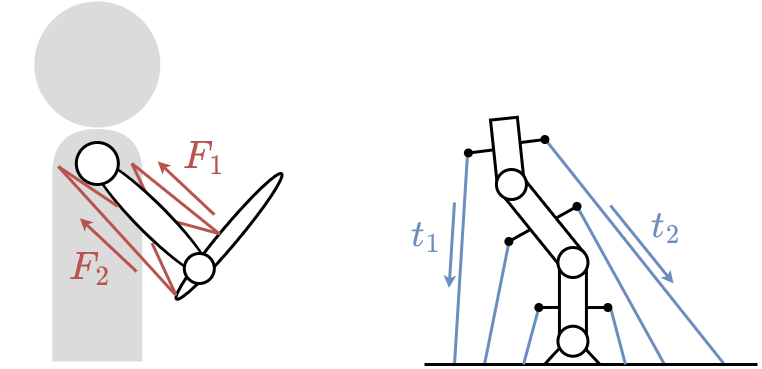
\includegraphics[width=\linewidth]{Chapters/imgs/muscle_mcdrs.png}
    \caption{An illustrative planar example of a human musculoskeletal model and a Multi-link cable-driven robot (MCDR). On the left human arm is modeled with two joints and six muscles, where each muscle can apply contraction forces $F_i$. On the right, a MCDR robot is modeled with 3 joints and 6 cables, which can apply tension forces $t_i$.  }
    \label{fig:muscle_mcdrs}
\end{wrapfigure}


 



One of the main differences comes from the actuator point of view. When it comes to MCDRs, the dynamics of the actuators is often neglected, considering them capable of instantaneously applying a range of $d$ tensile forces $\bm{t}\in\mathbb{R}^d$.
\begin{equation}
    \bm{t} \in [\bm{0},~\bm{t}_{max}]
\end{equation}
Additionally, this range is often considered constant and is not state dependent. For musculoskeleral models, on the other hand, the ranges of achievable muscle tension forces $\bm{F}$ are subject to many different biomechanical and biological factors, such as muscle length $\bm{l}$ and extension velocity $\dot{\bm{l}}$ as well the effects of fatigue and temperature.
Therefore the cables of the MCDRs can be seen as idealised muscles which tensile force capacity stays constant. 

Consequently, the physical ability metrics defined for the musculoskeleral models have the same formulation as the ones used to asses the performance of MCDRs.

\subsubsection{Wrench/Force polytope}
\label{ch:force_poly_human}
Task space force (or more generally wrench) capacity $\bm{f} \in \mathbb{R}^m$ is a well established metrics in biomechanics. It has been defined in two manners: a simplified formulation where the torques of $n$ human joints $\bm{\tau} \in \mathbb{R}^n$ are considered independent and limited (\ref{eq:human_torque_lim}) and in a more complete form where the human's joint torques $\bm{\tau}$ are generated by $d$ muscle tensile forces $\bm{F} \in \mathbb{R}^d$ which are limited in their respective ranges (\ref{eq:muslce_initial_range}).

Torque based polytopes \cite{rezzoug_application_2012,sasaki2011vertex} of achievable task space wrenches $\bm{f}$ have the same formulation as the force polytopes for robotic manipulators described in section \ref{ch:poly_force}. Therefore all the considerations for their evaluation are equivalent to those for robotic manipulators.  

However, real limits of human joint torques cannot be expressed as independent ranges (\ref{eq:human_torque_lim}) as they are generated by $d$ muscle tensile forces $\bm{F}$. The true limits of the joint torques $\bm{\tau}$ are polytope shaped as a consequence of the affine mapping of the muscle forces $\bm{F}$ to the joint space, though the moment arm matrix $N(\bm{q})=-L(\bm{q})^T$.
\begin{equation}
\mathcal{P}_\tau(\bm{q}) = \{\bm{\tau} \in \mathbb{R}^n ~|~\bm{F}\in [\bm{F}_{min}, \bm{F}_{max}], ~\bm{\tau}=N(\bm{q})\bm{F}\}
\label{eq:poly_torque_human}
\end{equation}

The relationship of the achievable task space wrenches $\bm{f}$ and the joint torques $\bm{\tau}$ is described through the dynamics equation 
\begin{equation}
\underbrace{M(\bm{q})\ddot{\bm{q}} + C(\bm{q},\dot{\bm{q}})\dot{\bm{q}} + \bm{g}(\bm{q})}_{\bm{\tau}_b(\bm{q},\dot{\bm{q}},\ddot{\bm{q}})} + J^T(\bm{q})\bm{f} = \bm{\tau} 
\end{equation}
where $\bm{\tau}_b(\bm{q},\dot{\bm{q}},\ddot{\bm{q}})$ is a state dependant joint torque bias vector including the influence of the gravity $\bm{g}(\bm{q})$ and human state $\{\dot{\bm{q}},\ddot{\bm{q}}\}$ and the desired acceleration $\ddot{\bm{q}}$. 

Finally the achievable set of task space wrenches $\bm{f}\in\mathbb{R}^m$ can then be expressed as a set of all the achievable wrenches $\bm{f}$ given the polytope $\mathcal{P}_\tau$ shaped limits of joint torques $\bm{\tau}$
\begin{equation}
    \mathcal{P}_f(\bm{q},\dot{\bm{q}},\ddot{\bm{q}}) = \left\{ \bm{f} \in \mathbb{R}^m ~|~ \bm{\tau}\in \mathcal{P}_\tau(\bm{q}), ~~ J^T(\bm{q})\bm{f} = \bm{\tau} -\bm{\tau}_b(\bm{q},\dot{\bm{q}},\ddot{\bm{q}}) \right\}
    \label{eq:human_force_poly_ver_poly_lim}
\end{equation}
Or in its implicit formulation
\begin{equation}
    \mathcal{P}_f(\bm{q},\dot{\bm{q}},\ddot{\bm{q}}) = \left\{ \bm{f} \in \mathbb{R}^m ~|~ \bm{F}\in\left[\bm{F}_{min}, \bm{F}_{max} \right], ~~ \!J^T(\bm{q})\bm{f} =\! N(\bm{q})\bm{F} -\bm{\tau}_b(\bm{q},\dot{\bm{q}},\ddot{\bm{q}}) \right\}
    \label{eq:human_force_poly}
\end{equation}

The final polytope formulation $\mathcal{P}_f$ has an implicit form composed of two affine mappings. First the limits of the muscle tension forces $\bm{F}\in \mathbb{R}^d$ are projected into the limits of the joint torques $\bm{\tau}\in \mathbb{R}^n$, then the polytope of the joint torques $\mathcal{P}_\tau$ is transformed to the task space wrenches $\bm{f}\in \mathbb{R}^m$ using the jacobian transpose matrix $J(\bm{q})^T$. As the musculoskeletal models often have large number of muscles $d$, the ending polytope $\mathcal{P}_f$ geometry is complex (having a large number of vertices and faces), both due to the number of muscles considered and the inherent complexity of the affine mapping. Therefore, this metric has been mostly used for static in-advance analysis of human postures \cite{hernandez_toward_2015}, due to its long execution times. 

However, Carmichael et al. \cite{carmichael_estimating_2013, carmichael2011Towards} have proposed a method capable of improving the time efficiency of the polytope resolution that has a potential to be used even in real-time applications. This method is based on Ray shooting method (RSM) that samples the polytope in a set of predefined direction in task space. By choosing the directions of interest in advance, the method is capable of approximating the polytope, however it does not give any guarantees on the approximation accuracy.

The achievable wrench polytope $\mathcal{P}_f$ formulation (\ref{eq:human_force_poly}) have been used for the analysis of the multi-link cable-driven robots (MCDRs) as well, for example in works by Sheng et al. \cite{sheng2020operational} or Muralidharan et al. \cite{Muralidharan2022}.

\subsubsection{Acceleration polytope}
\label{ch:human_aceleration_poly}

The task space acceleration polytope $\mathcal{P}_a$ describes the relationship between the limitation of the muscle tensile forces $\bm{F}\in \mathbb{R}^d$ and the set of achievable task space accelerations $\ddot{\bm{x}}\in\mathbb{R}^m$.

As in the case of the force polytope, the simplified approach to this metric is possible, where the human joint torque limits $\bm{\tau}\in\mathbb{R}^n$ are specified as independent ranges, resulting in the acceleration polytope formulation identical to the one for robotic manipulators, as introduced in section \ref{ch:accel_poly_robot}. 

However, human's joint torques $\bm{\tau}$ are not generated by a set of independent actuators, but with a set of $d$ contraction forces $\bm{F}$ produced by the muscle-tendon units $\bm{\tau}=N(\bm{q}) \bm{F}$. Therefore, real limits of achievable torques of human joints are polytope $\mathcal{P}_\tau$ shaped, as described by equation (\ref{eq:poly_torque_human}). 

The achievable acceleration polytope $\mathcal{P}_a$ formulation, respecting the muscle tension forces limits $\bm{F}$, can be derived from the human dynamics equation
\begin{equation}
M(\bm{q})\ddot{\bm{q}} + \underbrace{C(\bm{q},\dot{\bm{q}})\dot{\bm{q}} + \bm{g}(\bm{q}) + J^T(\bm{q})\bm{f}}_{\bm{\tau}_b(\bm{q},\dot{\bm{q}}, \bm{f})} = N(\bm{q}) \bm{F} 
\end{equation}
where $N(\bm{q})=-L(\bm{q})^T$ is the state dependant moment arm matrix. 
For any given human state $\{\bm{q},\dot{\bm{q}}, \bm{f}\}$, the effects of the human's motion, the gravity as well as the applied external wrenches, can be grouped in a constant torque vector $\bm{\tau}_b(\bm{q},\dot{\bm{q}},\bm{f})$. Then the actuator acceleration $\bm{q}$ can be expressed in relationship to the applied joint torque $\bm{\tau}$
\begin{equation}
    \ddot{\bm{q}} = M(\bm{q})^{-1}N(\bm{q})\bm{F} - M(\bm{q})^{-1}\bm{\tau}_b(\bm{q},\dot{\bm{q}}, \bm{f})
\end{equation}
Finally, the joint accelerations $\ddot{\bm{q}}$ can be transformed to the task space using the mapping (\ref{eq:js_to_cs_vaj_human:accel})
\begin{equation}
    \ddot{\bm{x}} = J(\bm{q})M(\bm{q})^{-1}N(\bm{q})\bm{F} - \underbrace{J(\bm{q})M(\bm{q})^{-1}\bm{\tau}_b(\bm{q},\dot{\bm{q}},\bm{f}) + \dot{J}(\bm{q}, \dot{\bm{q}})\dot{\bm{q}}}_{\bm{a}_b(\bm{q},\dot{\bm{q}},\bm{f})}
\end{equation}
where $\bm{a}_b(\bm{q},\dot{\bm{q}},\bm{f}) \in \mathbb{R}^m$ presents a constant bias vector for any human joint state $\{\bm{q},\dot{\bm{q}}\}$ and the genrated external wrench $\bm{f}$. The polytope $\mathcal{P}_a$ of achievable task space accelerations $\ddot{\bm{x}}$ can then be expressed as
\begin{equation}
\begin{split}
    \mathcal{P}_a(\bm{q},\dot{\bm{q}},\bm{f}) = \{ \ddot{\bm{x}} \in \mathbb{R}^m ~|~ \bm{F}&\in\left[\bm{F}_{min}, \bm{F}_{max} \right],\\ \ddot{\bm{x}} &= J(\bm{q})M(\bm{q})^{-1}N(\bm{q})\bm{F} - \bm{a}_b(\bm{q},\dot{\bm{q}},\bm{f}) \}
\end{split}
\label{eq:poly_acceleration_hum}
\end{equation}
The polytope $\mathcal{P}_a$ is formulated as a linear and affine projection of the muscles tension force $\bm{F}$ limits using the state dependant projection matrix $J(\bm{q})M(\bm{q})^{-1}N(\bm{q})$.  This polytope is much simpler to resolve than the force polytope $\mathcal{P}_f$ as it represents a projection of the $d$ dimensional limits of muscle tension forces $\bm{F}$ to the lower $m$ dimensional space of achievable task space accelerations $\ddot{\bm{x}}$.

Polytope $\mathcal{P}_a$ metrics have been used for musculoskeletal model analysis of highly dynamical movements such as football throwing \cite{khatib2009robotics} and golf swinging \cite{demircan2012muscle}. Additionally this metric has been used for the design analysis of the multi-link cable driven robots (MCDRs) as well \cite{sheng2020operational}.

\subsubsection{Velocity polytope}
\label{ch:human_vel_poly}
The simplest form of task space velocity capacity describes the relationship between the limited ranges (\ref{eq:human_js_vel_lim}) of human joint velocity $\dot{\bm{q}} \in \mathbb{R}^n$ and achievable task space velocities $\dot{\bm{x}} \in \mathbb{R}^m$, mapped through the jacobian matrix $J(\bm{q}) \in \mathbb{R}^{m\times n}$.
\begin{equation}
    \mathcal{P}_v(\bm{q}) = \left\{ \dot{\bm{x}} \in \mathbb{R}^m ~|~ \dot{\bm{q}}\in\left[\dot{\bm{q}}_{min}, \dot{\bm{q}}_{max} \right], ~~ \dot{\bm{x}} = J(\bm{q})\dot{\bm{q}} \right\}
\end{equation}
This formulation is essentially the same as the one for robotic manipulators described in velocity \ref{ch:vel_poly} and all the considerations discussed in that chapter are valid for this formulation as well.

However, taking in account only human's joint velocity $\dot{\bm{q}}$ limits in a form of independent ranges (\ref{eq:human_js_vel_lim}) does not take in consideration the limits of muscle extension velocity $\dot{\bm{l}}\in\mathbb{R}^d$. The true limits of human joint velocities are configuration dependent, as they are a consequence of the limits of muscle extension velocities $\dot{\bm{l}}$. The relationship between the joint and muscle extension velocities is given through the muscle jacobian matrix $L(\bm{q}) \in \mathbb{R}^{d\times n}$, forming polytope shaped limits
\begin{equation}
    \mathcal{P}_{\dot{q}}(\bm{q}) = \left\{ \dot{\bm{q}} \in \mathbb{R}^n ~|~ \dot{\bm{l}}\in\big[\dot{\bm{l}}_{min}, \dot{\bm{l}}_{max} \big], ~~ L(\bm{q})\dot{\bm{q}} = \dot{\bm{l}} \right\}
    \label{eq:human_poly_joint_vel}
\end{equation}
These polytope shaped limits can then be used to define the achievable task space velocity $\dot{\bm{x}}\in \mathbb{R}^m$ polytope which respects the limits of the muscle extension velocity $\dot{\bm{l}}$.
\begin{equation}
    \mathcal{P}_v(\bm{q}) = \left\{ \dot{\bm{x}} \in \mathbb{R}^m ~|~ \dot{\bm{q}}\in  \mathcal{P}_{\dot{q}}(\bm{q}), ~~ J(\bm{q})\dot{\bm{q}} = \dot{\bm{x}} \right\}
    \label{eq:velocity_polytope_human_ver_poly_lim}
\end{equation}
Or in its implicit form
\begin{equation}
    \mathcal{P}_v(\bm{q}) = \left\{ \dot{\bm{x}} \in \mathbb{R}^m ~|~ \dot{\bm{l}}\in\big[\dot{\bm{l}}_{min}, \dot{\bm{l}}_{max} \big], ~~ J(\bm{q})\dot{\bm{q}} = \dot{\bm{x}}, ~~ L(\bm{q})\dot{\bm{q}} = \dot{\bm{l}} \right\}
    \label{eq:velocity_polytope_human}
\end{equation}

This metric has an implicit formulation making its resolution relatively complex, requiring using multiple standard methods for polytope evaluation. It first requires finding the limits of joint velocities $\dot{\bm{q}} \in \mathbb{R}^n$ based on the limits of the muscle extension velocities $\dot{\bm{l}} \in \mathbb{R}^d$ and then projecting them to the task space velocities $\dot{\bm{x}} \in \mathbb{R}^m$. 

To the best of our knowledge, polytope $\mathcal{P}_v$ in its full implicit form (\ref{eq:velocity_polytope_human}), has not yet been used with musculoskeletal models. However, achievable velocity based physical ability metrics such as manipulability ellipsoids considering the joint velocity $\dot{\bm{q}}$ limits \cite{Chiu1988,Petric2019,Yang2017}, have been used in the human motion and ergonomics analysis. However, as these metrics neglect the the muscle extension velocity $\dot{\bm{l}}$ limits, polytope $\mathcal{P}_v$ could be used as their more complete alternative. 

The achievable velocity polytope $\mathcal{P}_v$, in the form (\ref{eq:velocity_polytope_human}), has been used for multi-link cable driven robots (MCDRs) analysis \cite{Muralidharan2022}.

\subsubsection{Stiffness polytope}
\label{ch:human_stiffness_poly}
Stiffness metrics for human musculoskeletal models are used to evaluate the limitations of the endpoint displacement $\Delta x \in \mathbb{R}^m$ given the known muscle stiffness matrix $K_m \in \mathbb{R}^{d\times d}$ and a limited range of task space wrenches $\bm{f} \in \mathbb{R}^m$. 

\begin{equation}
    \bm{f}\in\left[\bm{f}_{min}, \bm{f}_{max} \right]
    \label{eq:force_stiff_range_human}
\end{equation}

With a known muscle stiffness matrix $K_m$, that can be determined using the Hill's muscle model \cite{LATASH1993653}, the joint stiffness matrix $K_j\in \mathbb{R}^{n\times n}$ can be found using the muscle jacobian matrix $L(\bm{q}) \in \mathbb{R}^{d\times n}$
\begin{equation}
    K_j = L(\bm{q}) K_m L(\bm{q})^T 
\end{equation}
This joint space stiffness matrix $K_j$ can be used to find the robot state dependent task space stiffness $K_c  \in \mathbb{R}^{m\times m}$, through the jacobian matrix $J(\bm{q})\in\mathbb{R}^{m\times n}$  \cite{Salisbury1980,Ajoudani2018,Inouye2016}
\begin{equation}
     K_c(\bm{q})^{-1} = J(\bm{q}) K_j^{-1}J(\bm{q})^T
\end{equation}
Given the range of expected external wrenches (\ref{eq:force_stiff_range_human}), the polytope of maximal task space displacements $\Delta\bm{x}$ can then be expressed as
\begin{equation}
    \mathcal{P}_\Delta(\bm{q}) = \left\{ \Delta\bm{x} \in \mathbb{R}^m ~|~ \bm{f}\in\left[\bm{f}_{min}, \bm{f}_{max} \right], ~~ K_c(\bm{q})\Delta\bm{x} = \bm{f} \right\}
    \label{eq:stiffness_human_simple}
\end{equation}


However, this formulation considers that the external wrench $\bm{f}$ range (\ref{eq:force_stiff_range_human}) is inside the human wrench capacity. In order to make sure that the human's wrench capacity is not exceeded when calculating the maximal task space displacement polytope $\mathcal{P}_\Delta$ the external wrench range (\ref{eq:force_stiff_range_human}) needs to be intersected with the human's wrench polytope  $\mathcal{P}_f$ described in the section \ref{ch:force_poly_human}, the polytope $\mathcal{P}_\Delta$ of task space task space displacement $\Delta \bm{x}$ can then be expressed as
\begin{equation}
    \mathcal{P}_\Delta(\bm{q},\dot{\bm{q}},\ddot{\bm{q}}) = \left\{ \Delta\bm{x} \in \mathbb{R}^m ~|~ \bm{f}\in \left[\bm{f}_{min}, \bm{f}_{max} \right] \cap \mathcal{P}_f(\bm{q},\dot{\bm{q}},\ddot{\bm{q}}),  ~~ \! K_c(\bm{q})\Delta\bm{x}=\bm{f}\right\}
\end{equation}

If the maximal displacement polytope $\mathcal{P}_\Delta$ is calculated only in relationship to the human's wrench capacity $\mathcal{P}_f$, without specifying the expected range of external wrenches (\ref{eq:force_stiff_range_human}), this polytope can be expressed in an implicit form
\begin{equation}
\begin{split}
    \mathcal{P}_\Delta(\bm{q},\dot{\bm{q}},\ddot{\bm{q}}) =\! \{ \Delta\bm{x} \in \mathbb{R}^m ~|&\bm{F}\in\left[\bm{F}_{min}, \bm{F}_{max} \right]\!,\\ ~ &J^T(\bm{q})K_c(\bm{q})\Delta\bm{x}\!= N(\bm{q})\bm{F}\! -\! \bm{\tau}_b(\bm{q},\dot{\bm{q}},\ddot{\bm{q}}) \}\label{eq:stiffness_human_all}
\end{split}
\end{equation}
The stiffness polytope $\mathcal{P}_\Delta$ then represents the maximal task space displacement $\Delta \bm{x} \in \mathbb{R}^m$ that can be achieved given the human's muscle tensile forces $\bm{F} \in \mathbb{R}^d$ limits (\ref{eq:muslce_initial_range}), this polytope formulation is also called \textit{stiffness feasibility region} \cite{ajoudani2017choosing}.

The formulation of the polytope (\ref{eq:stiffness_human_simple}) has relatively low complexity, defined as a projection of the limits of the external task space wrenches $\bm{f} \in \mathbb{R}^m$ to the same dimensional task space displacements $\Delta \bm{x} \in \mathbb{R}^m$. However, the implicit polytope formulation (\ref{eq:stiffness_human_all}) is much more complex as the limits of muscle tension forces $\bm{F} \in \mathbb{R}^d$ first need to be projected to the limits of the joint torques $\bm{\tau} \in \mathbb{R}^n$ which in term determine the set of task space displacements $\Delta \bm{x} \in \mathbb{R}^m$. While the formulation  (\ref{eq:stiffness_human_simple}) can be resolved with standard polytope resolution algorithms, the formulation (\ref{eq:stiffness_human_all}) requires a combination of multiple methods, making it significantly more time consuming. 

These polytope based metrics however, to the best of our knowledge, have yet to be used with human musculoskeletal models and MCDRs. However, their potential has already been shown for human posture analysis \cite{Inouye2016} and MCDR design \cite{Ramadoss2021} applications, in their simplified ellipsoid forms.

\section{Polytope representation of collaboration abilities}
\label{ch:collab_metrics}

\begin{figure}[!h]
    \centering
    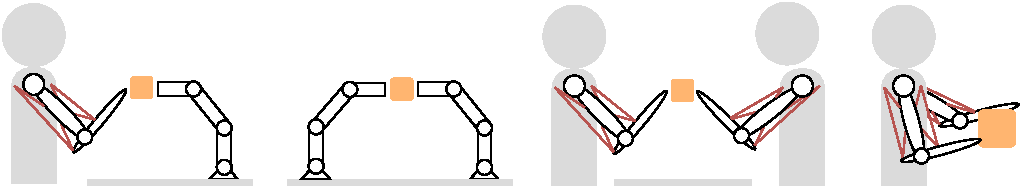
\includegraphics[width=\linewidth]{Chapters/imgs/collaboration.pdf}
    \caption{Illustrative examples of a common collaboration scenario composed of different actors (humans and robots), from left to right, human-robot, robot-robot, human-human and even two arms of a human subject can be seen as a collaboration of two musculoskeletal models.}
    \label{fig:collaboration_types}
\end{figure}

Physical ability metrics are an important tool for analysing how robots and humans comply with different requirements of tasks. In human-robot collaboration scenarios, these metrics can be used is to decide if the robot, or the human, is better suited to execute a certain task, by evaluating their different physical abilities (movement, forces, precision etc.) to the ones required by the task\cite{Edoardo2019Capability}. 

However, when it comes to the physical collaboration, where the task is executed jointly by the human and the robot physically interacting, expressing their common physical abilities is much more challenging. As their common physical ability is a combination of their individual abilities, to be able to calculate their common physical ability, they need to be expressed in a unified form.  

Many different physical abilities for humans and robots, can be represented in the polytope form, as described in section \ref{ch:poly_metrics}. Expressing their physical abilities in this unifying form enables using different efficient tools from the polytope algebra to combine their individual polytopes, such as Minkowski sums, intersections and convex-hulls.
Therefore, given their individual polytopes of different physical abilities and the physics of their physical interaction scenario, different polytope algebra operations can be leveraged to express their common physical ability in the polytope form as well.

One example of such characterisation has been developed by Jihong Lee, in his work \cite{lee2001velocity}, showing how polytopes can be used to describe the common velocity capacity of multi-arm collaborative robotic system, by intersecting their individual polytopes. However, this approach is yet to used for characterising the common capacity of the human-robot interaction, as well as to be extended to other physical abilities and other collaboration scenarios. 


Therefore, following sections describe the characterisation of different common physical abilities of the human-robot interaction, based on one classical example of human-robot collaboration scenario, where the two actors interact physically to manipulate an object that is rigidly fixed in the end-effector of the robot and in the hand of the human. First, section \ref{ch:which_metric_which} introduces the physical relationships describing this collaboration scenario, followed by the two sections, \ref{ch:force_collab} and \ref{ch:velocity_collab}, giving more specific examples of how these relationships are exploited to calculate the common force and velocity capacity of a physical human-robot collaboration leveraging the polytope algebra. 
Different versions of this scenario are shown on Figure \ref{fig:collaboration_types}, ranging from human-robot interaction to the interaction of the two arms of a human subject, that can be seen as two separate musculoskeletal models collaborating.

\todos{Even though the following sections are focusing on one collaboration scenario, similar approach can be used to characterising any other collaboration scenario as well.}

\subsection{Human-robot collaboration scenario}
\label{ch:which_metric_which}
\begin{wrapfigure}{r}{0.5\textwidth}
    \centering
    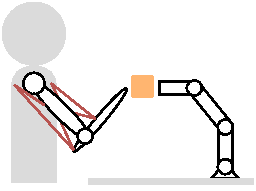
\includegraphics{Chapters/imgs/example_inter.pdf}
    \caption{A collaborative example scenario where a human and a robot interact over an object fixed rigidly in the end-effector of the robot and in the hand of the human.}
    \label{fig:table_inter}
\end{wrapfigure}

A classical human-robot physical interaction scenario is considered, where the human operator and the robot are physically interacting in order to manipulate an object which is rigidly fixed both in the robot's end-effector and the human's hand. A simplified view of this collaboration scenario is shown on Figure \ref{fig:table_inter}, while a more general view of this scenario, with different actors (humans and robots), is shown on Figure \ref{fig:collaboration_types}.

When it comes to commonly manipulating an object held by both human and the robot, the supposition of rigid contact with the object can be used to formulate the force equilibrium equation and the relative motion constraints \cite{Prattichizzo2016}. 

As they both apply forces on the object, the resulting force $\bm{f}$ the object will exert on the environment (if in contact with it) or transform into motion follows from the force equilibrium ( sum of all forces $\bm{f}_i$ is equal to zero ), and is equal to the sum of the applied forces by the robot $\bm{f}_r$ and the human $\bm{f}_h$. 
\begin{equation}
    \bm{f} = \bm{f}_r + \bm{f}_h, \qquad  m_o\ddot{\bm{x}} = \bm{f} 
\end{equation}
If the object is not in contact with the environment, the force $\bm{f}$ will generate object's acceleration $\ddot{\bm{x}}$  in space proportional to its mass $m_o$.

Furthermore, as the object is rigidly attached to both robot and the human, there is no relative movement possible between the object, human's hand and robot's end-effector. According to this condition, the movement of the object (velocity $\dot{\bm{x}}$, acceleration $\ddot{\bm{x}}$, jerk $\dddot{\bm{x}}$, etc.) is equivalent to the movement of both the human's hand $\{\dot{\bm{x}}_h,\ddot{\bm{x}}_h,\dddot{\bm{x}}_h\}$ and the robot's end-effector $\{\dot{\bm{x}}_r,\ddot{\bm{x}}_r,\dddot{\bm{x}}_r\}$.
\begin{equation}
    \dot{\bm{x}}_h=\dot{\bm{x}}_r=\dot{\bm{x}}, \qquad
    \ddot{\bm{x}}_h=\ddot{\bm{x}}_r=\ddot{\bm{x}}, \qquad
    \dddot{\bm{x}}_h=\dddot{\bm{x}}_r=\dddot{\bm{x}}
    \label{eq:kinematic_condition_contact}
\end{equation}

These two relationships, considering the rigid contact between the robot, human and the object, can be used to describe different physical abilities of the human-robot collaboration in the described scenario. Section \ref{ch:force_collab} describes exploiting this relationship to calculate the common force capacity while section \ref{ch:velocity_collab} described the calculation of their common velocity capacity.


% where each one of the forces is bounded in withing the polytope $\bm{f}_i \in \mathcal{P}_{fi}$. 
% \begin{equation}
%     \mathcal{P}_f = \{\bm{f}\in \mathbb{R}^m ~|~\bm{f} = \bm{f}_r + \bm{f}_h , \quad\bm{f}_r \in \mathcal{P}_{fr},~\bm{f}_h \in \mathcal{P}_{fh}\}
% \end{equation}
% Therefore their common wrench capacity can be expressed as a sum of their individual wrench capacities, corresponding to the Minkowski sum $\oplus$ in polytope algebra 
% \begin{equation}
%     \mathcal{P}_f = \mathcal{P}_{fr}\oplus \mathcal{P}_{fh}
% \end{equation}


% %the maximal velocity capacity of the object will be limited by the actor (human or robot) with the least velocity capacity. 

% On the other hand, in the proposed collaboration scenario, as both robot and the human are rigidly attached to the object, the velocity of the object $\dot{\bm{x}}$ is equal to the velocity of the human's hand $\dot{\bm{x}}_h$ and the robot's end-effector $\dot{\bm{x}}_r$ \cite{Prattichizzo2016}
% \begin{equation}
%     \dot{\bm{x}}_h=\dot{\bm{x}}_r=\dot{\bm{x}}
%     \label{eq:kinematic_condition_contact}
% \end{equation}
% as both of them have their own limited velocity capacity $\dot{\bm{x}}_h \in \mathcal{P}_{vh},\dot{\bm{x}}_r \in \mathcal{P}_{vr}$ the object velocity has to respect all of them
% \begin{equation}
%     \mathcal{P}_v = \{\dot{\bm{x}}\in \mathbb{R}^m ~|~ \dot{\bm{x}} \in \mathcal{P}_{vr},~\dot{\bm{x}} \in \mathcal{P}_{vh}\}
% \end{equation}
% Geometrically, this operation can be represented as an intersection of their velocity capacities, and the intersection $\cap$ operation can be calculated efficiently using polytope algebra. 
% \begin{equation}
%     \mathcal{P}_v =  \mathcal{P}_{vh} \cap \mathcal{P}_{vr}
% \end{equation}



% More generally, all the polytope formulations that require calculating the wrench/force capacity, for both robot's and human's, will be combined using Minkowski sum $\oplus$. Such metrics are human's and robot's wrench/force polytope and stiffness region polytope.

% More generally, all polytope metrics characterising robot's or human's movement capacity (velocity $\dot{\bm{x}}$, acceleration $\ddot{\bm{x}}$, etc.) will be subject to the same condition (\ref{eq:kinematic_condition_contact}) and will be combined using the intersection $\cap$ operation.




% The further discussed procedures for calculating joint physical ability polytopes are valid for the considered collaboration scenario (showed on Figure \ref{fig:table_inter} or more generally on Figure \ref{fig:collaboration_types}), however the same methodology can be used to any other collaboration scenario as well.

% \begin{table}
% \centering
% \begin{tabular}{|l|c | c| c| c|}
% \hline
% Polytope Metric & Equation & Dynamics & Collaboration operator \\
% \hline
%  \multicolumn{5}{c}{Robotic manipulators }  \\
% \hline
% Velocity  &  \ref{eq:poly_vel_rob}& No & $\cap$ \\
% Kinematic Acceleration  & \ref{eq:poly_accel_kin} & No & $\cap$ \\
% Kinematic Jerk  &  \ref{eq:poly_jerk_kin}& No &  $\cap$ \\
% Precision  & \ref{eq:poly_precision_rob} & No&  $\cap$ \\
% Force/Wrench  & \ref{eq:poly_force_rob} & Yes &$\oplus$ \\
% Acceleration  & \ref{eq:pol_accleration_rob} & Yes &   $\cap$ \\
% Stiffness feasibility  &  \ref{eq:pol_sfr_rob} & Yes& $\oplus$ \\
% \hline
%  \multicolumn{5}{c}{Human musculoskeletal models}  \\
% \hline
% Velocity  & \ref{eq:velocity_polytope_human} & No &  $\cap$ \\
% Force/Wrench & \ref{eq:human_force_poly} & Yes & $\oplus$ \\
% Acceleration  & \ref{eq:poly_acceleration_hum} & Yes &  $\cap$ \\
% Stiffness feasibility  & \ref{eq:stiffness_human_all}  & Yes&  $\oplus$ \\
% \hline
% \end{tabular}
% \caption{The list of common polytope based physical ability metrics alongside their polytope algebra operator for the example collaborative scenario (Figure \ref{fig:table_inter}), as well as the indication of their capacity to account for the dynamics effects.}
% \label{tab:table_comparisson_colloboration}
% \end{table}


\subsection{Force polytope}
\label{ch:force_collab}
\begin{figure}[!h]
    \centering
    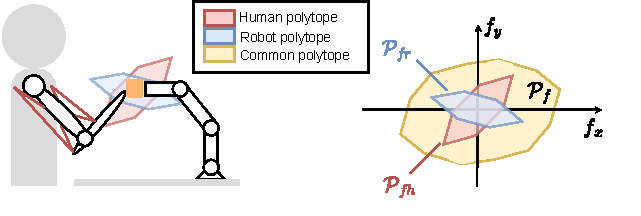
\includegraphics[width=0.7\linewidth]{Chapters/imgs/force_collab.pdf}
    \caption{A collaborative example scenario where a human and a robot interact over an object fixed rigidly in the end-effector of the robot and in the hand of the human. The force polytope of the human (red) and the robot (blue) as well as their collaborative polytope (orange) calculated as a Minkowski sum of their individual polytopes are shown on the right.}
    \label{fig:collaboration_force}
\end{figure}

When a human operator and a robot are physically interacting in order to manipulate an object, which is rigidly fixed both in the robot's end-effector and the human hand, the final force exerted on the object will be the sum of the forces of the human $\bm{f}_h$ and the force of the robot $\bm{f}_r$.
\begin{equation}
    \bm{f} = \bm{f}_h + \bm{f}_r
\end{equation}

Their individual force capacity can be expressed in a polytope form, for the human  $\mathcal{P}_{fh}$ and the robot  $\mathcal{P}_{fr}$ respectively. Finally, as their forces acting on the object are summed, their common force capacity on the object can be expressed as
\begin{equation}
    \mathcal{P}_f = \{\bm{f}\in \mathbb{R}^m ~|~\bm{f} = \bm{f}_r + \bm{f}_h , \quad\bm{f}_r \in \mathcal{P}_{fr},~\bm{f}_h \in \mathcal{P}_{fh}\}
\end{equation}
Therefore their common wrench capacity can be expressed as a sum of their individual wrench capacities, corresponding to the Minkowski sum $\oplus$ in polytope algebra 
\begin{equation}
    \mathcal{P}_f = \mathcal{P}_{fr}\oplus \mathcal{P}_{fh}
\end{equation}

A planar example of this collaboration scenario and the polytopes obtained is in shown on Figure \ref{fig:collaboration_force}. 

In more general case, if a collaboration is composed of $N$ actors rigidly holding an object, where their force capacity is expressed in a polytope form $\mathcal{P}_{fi}$, then their common force capacity can be calculated as the Minkowski sum of the $N$ polytopes.

\begin{equation}
    \mathcal{P}_f =  \mathcal{P}_{f1} \oplus \mathcal{P}_{f2} \oplus ~\ldots ~\oplus  \mathcal{P}_{fN}
\end{equation}

Furthermore, the polytope formulations that require calculating the wrench/force capacity, for both robot's and human's, will be combined using Minkowski sum $\oplus$. Such metrics are human's and robot's wrench/force polytope and stiffness region polytope, as shown in table \ref{tab:merged_table}.

\subsection{Velocity polytope}
\label{ch:velocity_collab}

\begin{figure}[!h]
    \centering
    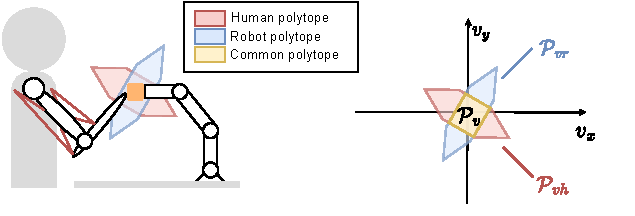
\includegraphics[width=0.7\linewidth]{Chapters/imgs/velocity_collab.pdf}
    \caption{A collaborative example scenario where a human and a robot interact over an object fixed rigidly in the end-effector of the robot and in the hand of the human. The velocity polytope of the human (red) and the robot (blue) as well as their collaborative polytope (orange) calculated as an intersection of their individual polytopes are shown on the right.}
    \label{fig:collaboration_vel}
\end{figure}

When a human operator and a robot are physically interacting in order to manipulate an object which is rigidly fixed both in the robot's end effector and the human hand, there is no relative movement of the object with respect to the human's hand and the robot's end effector
\begin{equation}
    \dot{\bm{x}}_h=\dot{\bm{x}}_r=\dot{\bm{x}},
\end{equation}

Once their individual velocity capacity is expressed in polytope form $\mathcal{P}_{vh}$ and $\mathcal{P}_{vr}$, their common velocity capacity $\mathcal{P}_v$ (the achievable velocities of the object) can then be calculated as 
\begin{equation}
    \mathcal{P}_v = \{\dot{\bm{x}}\in \mathbb{R}^m ~|~ \dot{\bm{x}} \in \mathcal{P}_{vr},~\dot{\bm{x}} \in \mathcal{P}_{vh}\}
\end{equation}
Geometrically, this operation can be represented as an intersection of their velocity capacities, and the intersection $\cap$ operation can be calculated efficiently using polytope algebra. 
\begin{equation}
    \mathcal{P}_v =  \mathcal{P}_{vh} \cap \mathcal{P}_{vr}
\end{equation}

A planar example of this collaboration scenario and the polytopes obtained is in shown on Figure \ref{fig:collaboration_vel}. 


% The maximal velocity the object can achieve in a certain direction $\bm{v}_{max}$ will be limited by the actor who has the lower maximal velocity in that direction. It can be found as the minimum value of the maximal velocity the human arm can achieve $\bm{v}_{h,max}$ and the robot's end-effector can achieve $\bm{v}_{r,max}$
% \begin{equation}
%     \bm{v}_{max}= \min \{\bm{v}_{h,max}, \bm{v}_{r,max}\}
% \end{equation}

In a more general case where there are $N$ actors (robots and humans) collaborating by rigidly holding the object, and where their velocity capacity is expressed in a polytope form $\mathcal{P}_{vi}$, the common velocity capacity can be calculated as their intersection
\begin{equation}
    \mathcal{P}_v =  \mathcal{P}_{v1} \cap \mathcal{P}_{v2} \cap ~~ \ldots ~~\cap \mathcal{P}_{vN}
\end{equation}

Furthermore, the polytope formulations characterising robot's or human's movement capacity (velocity $\dot{\bm{x}}$, acceleration $\ddot{\bm{x}}$, etc.) will be subject to the same condition (\ref{eq:kinematic_condition_contact}) and will be combined using the intersection $\cap$ operation, as shown in table \ref{tab:merged_table}.

\section{Conclusion and synthesis}
\label{ch:collab_metrics_overview}

This chapter brings an overview of different ways of characterising physical abilities for humans and robots, with the aim to find a unified view of their abilities and provide a base for characterising their common physical abilities. Even though many different metrics have been developed for human and robot physical ability characterisation, they are often very different in scope, accuracy, physical interpretation and in many cases specific to only robots or only humans. The focus of this chapter, as well as this thesis, is therefore placed on polytope based representations of physical abilities as they are arguably the most complete and the most accurate characterisations for both robots and humans, based on their musculoskeletal models.

An overview of the common polytope based representations of humans' and robots' physical abilities is then provided in section \ref{ch:poly_metrics}, in the attempt to present a systematic view on their formulations. In this overview, different physical abilities of humans (based on musculoskeletal models) and robots are characterised by finding the relationships between their actuation limits and the achievable sets of different task-related variables. As these relationships are usually described through robot's and human's highly nonlinear dynamics and kinematics relationships, in order to obtain the polytope-shaped representations, the dynamics and kinematics equations are linearised around a specific state, yielding linear and affine transformations of the actuator limits to the achievable sets of desired task space variables.

Common polytope formulations, described in section \ref{ch:robot_metrics} for robots and in section \ref{ch:human_metrics} for humans, involve different linearised dynamics and kinematics equations, as well as different actuation limits. However, they can be represented using a generic formulation
\begin{equation}
    \mathcal{P}_x = \{\bm{x}\in\mathbb{R}^m ~|~ A\bm{x}=B\bm{y} + \bm{b}, ~ \bm{y}\in\mathcal{P}_y\}
    \label{eq:generic_polyt_view}
\end{equation}
where the polytope $\mathcal{P}_x$ represents the achievable set of the task space variable $\bm{x}\in\mathbb{R}^m$, $\bm{y}\in\mathbb{R}^k$ is the input (actuator) variable limited within input set (actuator limits) $\mathcal{P}_y$. The input set $\mathcal{P}_y$ is often defined in the form of intervals of different input (actuator) variables, however in general case it can have a polytope shape as well. The linearised dynamics and kinematics equations can be represented, in a generic case, using the equation $A\bm{x}\!=\!B\bm{y}\!+\!\bm{b}$, where the matrix $A\in\mathbb{R}^{k\times m}$ is a linear transformation matrix from the $m$ dimensional output (task) space to the $k$ dimensional intermediate space, the matrix $B\in\mathbb{R}^{k\times d}$ is a transformation matrix from the $n$ dimensional input space to the intermediate space and the $\bm{b}\in\mathbb{R}^k$ is a bias vector expressed in the intermediate space. Furthermore, the dimensions of output (task) space $m$ is lower than the intermediate space dimension $k\!\geq\! m$ , which is in term lower than the input (actuator) space dimension $n\!\geq\! k\!\geq\! m$. This condition comes from the fact that when characterising the physical abilities, the polytopes map higher dimensional input space (ex. joint space or muscle force space) to the lower dimensional output space (ex. Cartesian space).

\begin{table}[!b]
\scalefont{0.9}
\centering
\begin{tabular}{|l|c|c|c|c|c|c|c|c|c|}
\hline
Polytope capacity & Eqn. & $\bm{x}$ & $A$ & $B$ & $\bm{y}$ & Input set $\mathcal{P}_y$ & $\bm{b}$ & Cond. & Collab. \\
\hline
\multicolumn{10}{c}{Robotic manipulators} \\
\hline
Velocity & \ref{eq:poly_vel_rob}& $\dot{\bm{x}}$ & $I_{m\times m}$ & $J$ & $\dot{\bm{q}}$& $[\dot{\bm{q}}_{min},\dot{\bm{q}}_{max}]$ & - & Kin & $\cap$ \\
Kin. Acceleration & \ref{eq:poly_accel_kin} & $\ddot{\bm{x}}$ & $I_{m\times m}$ & $J$ & $\ddot{\bm{q}}$ & $[\ddot{\bm{q}}_{min},\ddot{\bm{q}}_{max}]$ & $\bm{a}_b$ & Kin & $\cap$ \\
Kin. Jerk &\ref{eq:poly_jerk_kin} & $\dddot{\bm{x}}$ & $I_{m\times m}$ & $J$ & $\dddot{\bm{q}}$& $[\dddot{\bm{q}}_{min},\dddot{\bm{q}}_{max}]$ & $\bm{j}_b$ & Kin & $\cap$ \\
Precision & \ref{eq:poly_precision_rob} & $\delta\dot{\bm{x}}$ & $I_{m\times m}$ & $J$ & $\delta\bm{q}$ &$[\delta{\bm{q}}_{min},\delta{\bm{q}}_{max}]$ & - & Kin & $\cap$ \\
Force/Wrench & \ref{eq:poly_force_rob} & $\bm{f}$ & $J^T$ & $I_{n\times n}$ & $\bm{\tau}$ &$[\bm{\tau}_{min},\bm{\tau}_{max}]$ & -$\bm{\tau}_b$ & Dyn & $\oplus$ \\
Acceleration & \ref{eq:pol_accleration_rob} & $\ddot{\bm{x}}$ & $I_{m\times m}$ & $JM^{-1}$ & $\bm{\tau}$ &$[\bm{\tau}_{min},\bm{\tau}_{max}]$ & -$\bm{a}_b$ & Dyn & $\cap$ \\
Stiffness & \ref{eq:pol_sfr_rob}& $\Delta\bm{x}$ & $J^TK_c$ & $I_{n\times n}$ & $\bm{\tau}$ &$[\bm{\tau}_{min},\bm{\tau}_{max}]$ & -$\bm{\tau}_b$ & Dyn & $\oplus$ \\
\hline
\multicolumn{10}{c}{Human musculoskeletal models} \\
\hline
Velocity &\ref{eq:velocity_polytope_human} & $\dot{\bm{x}}$ & $I_{m\times m}$ & $J$ & $\dot{\bm{q}}$ & $\mathcal{P}{\dot{\bm{q}}}$ & - & Kin & $\cap$ \\
Force/Wrench & \ref{eq:human_force_poly} & $\bm{f}$ & $J^T$ & $N$ & $\bm{F}$ & $[\bm{F}_{min},\bm{F}_{max}]$ & -$\bm{\tau}_b$ & Dyn & $\oplus$ \\
Acceleration & \ref{eq:poly_acceleration_hum} & $\ddot{\bm{x}}$ & $I_{m\times m}$ & $JM^{-1}N$ & $\bm{F}$ & $[\bm{F}_{min},\bm{F}_{max}]$ & -$\bm{a}_b$ & Dyn & $\cap$ \\
Stiffness & \ref{eq:stiffness_human_all} &$\Delta\bm{x}$ & $J^TK_c$ & $N$ & $\bm{F}$ & $[\bm{F}_{min},\bm{F}_{max}]$ & -$\bm{\tau}_b$ & Dyn & $\oplus$ \\
\hline
\end{tabular}
\caption{The list of common polytope formulations for characterising physical abilities of robots and humans introduced in section \ref{ch:poly_metrics}. The table shows the correspondence of the common formulations to the generic formulation described by the equation (\ref{eq:generic_polyt_view}). The table further specifies if the polytope formulations is specified in kinematic or dynamic conditions. Finally, the table shows the necessary polytope algebra operator in order to characterise the common abilities in the collaboration scenario described in section \ref{ch:which_metric_which}.}
\label{tab:merged_table}
\end{table}

Table \ref{tab:merged_table} brings a list of the polytope formulations for robots and humans, introduced in section \ref{ch:poly_metrics}, in a condensed view. The table brings shows how different polytope formulations correspond with the generic polytope formulation (\ref{eq:generic_polyt_view}), in terms of system matrices $A,B$, input, output and bias vectors $\bm{x},\bm{y},\bm{b}$ and the input limits $\mathcal{P}_y$.

Polytopes, apart from being able to accurately represent both human's and robot's physical abilities, enable combining their individual polytopes for characterising the common physical abilities when interacting physically to execute different task. Given the physical ability of interest and the physics of the human-robot physical interaction scenario, different polytope algebra tools, such as Minkowski sum or intersection, can be used to express the common physical ability of their interaction in the polytope form as well.


Section \ref{ch:collab_metrics}, demonstrates the use of different polytope algebra operations to characterise force and movement capacity of the human-robot collaboration in one classical collaboration scenario, where the human and the robot jointly manipulate an object. In the context of the same scenario, table \ref{tab:merged_table} shows the polytope algebra operators (Minkowski sum $\oplus$ and intersection $\cap$) used to combine their individual polytopes to characterise their different physical abilities as one system.


In summary, polytopes enable accurate representation of human's and robot's physical abilities, as well as characterising their common physical abilities when collaborating physically to execute a task. In that way, this representation provides tools to create more advanced collaboration scenarios. 
Accurate representation of robot's physical abilities enables exploiting its abilities fully when designing its tasks, creating the adapted robot control strategies or planning for its trajectories. On the other hand, accurate representation of human's abilities enables assessing the task ergonomics and making sure that human's capacity is never surpassed. Additionally, it enables creating more human-centered robot behaviours, where the robot adapts its assistance level to the lacking physical abilities of the human operator. 
Finally, a unified representation of their individual and common physical abilities might enable new task scheduling techniques capable of assessing if different tasks are more suitable for robots, human operators or are they more suitable for their collaboration. 

However, polytope formulations, as introduced in section \ref{ch:poly_metrics}, need to be transformed to more standard representations in order to  be used in practical implementations. The two most common ways to represent a polytope are as a set of vertices, or as a set of inequality constraints corresponding to its faces. Depending on the polytope formulation structure different transformation strategies, to the one of these forms, need to be employed, where the computational efficiency of the transformation operation can vary significantly with respect to the formulation complexity. Therefore following chapter focuses on providing a generic view on different formulation families present when characterising physical abilities of humans and robots, with the aim to specify different polytope transformation strategies applicable to each of the families as well as to discuss their computational complexity.


% \pagebreak

% \begin{landscape}
% \centering
% \begin{table}[!h]
% \centering
% \begin{tabular}{|l|c|c|c|c|c|c|c|c|c|}
% \hline
% Polytope capacity & Equation & $\bm{x}$ & $A$ & $B$ & $\bm{y}$ & Input set $\mathcal{I}$ & $\bm{b}$ & Conditions & Collaboration \\
% \hline
% \multicolumn{10}{c}{Robotic manipulators} \\
% \hline
% Velocity & \ref{eq:poly_vel_rob}& $\dot{\bm{x}}$ & - & $J$ & $\dot{\bm{q}}$& $[\dot{\bm{q}}_{min},\dot{\bm{q}}_{max}]$ & - & Kin & $\cap$ \\
% Kin. Acceleration & \ref{eq:poly_accel_kin} & $\ddot{\bm{x}}$ & - & $J$ & $\ddot{\bm{q}}$ & $[\ddot{\bm{q}}_{min},\ddot{\bm{q}}_{max}]$ & $\bm{a}_b$ & Kin & $\cap$ \\
% Kin. Jerk &\ref{eq:poly_jerk_kin} & $\dddot{\bm{x}}$ & - & $J$ & $\dddot{\bm{q}}$& $[\dddot{\bm{q}}_{min},\dddot{\bm{q}}_{max}]$ & $\bm{j}_b$ & Kin & $\cap$ \\
% Precision & \ref{eq:poly_precision_rob} & $\delta\dot{\bm{x}}$ & - & $J$ & $\delta\bm{q}$ &$[\delta{\bm{q}}_{min},\delta{\bm{q}}_{max}]$ & - & Kin & $\cap$ \\
% Force/Wrench & \ref{eq:poly_force_rob} & $\bm{f}$ & $J^T$ & - & $\bm{\tau}$ &$[\bm{\tau}_{min},\bm{\tau}_{max}]$ & -$\bm{\tau}_b$ & Dyn & $\oplus$ \\
% Acceleration & \ref{eq:pol_accleration_rob} & $\ddot{\bm{x}}$ & - & $JM^{-1}$ & $\bm{\tau}$ &$[\bm{\tau}_{min},\bm{\tau}_{max}]$ & -$\bm{a}_b$ & Dyn & $\cap$ \\
% Stiffness & \ref{eq:pol_sfr_rob}& $\Delta\bm{x}$ & $J^T$ & - & $\bm{\tau}$ &$[\bm{\tau}_{min},\bm{\tau}_{max}]$ & -$\bm{\tau}_b$ & Dyn & $\oplus$ \\
% \hline
% \multicolumn{10}{c}{Human musculoskeletal models} \\
% \hline
% Velocity &\ref{eq:velocity_polytope_human} & $\dot{\bm{x}}$ & - & $J$ & $\dot{\bm{q}}$ & $\mathcal{P}{\dot{\bm{q}}}$ & - & Kin & $\cap$ \\
% Force/Wrench & \ref{eq:human_force_poly} & $\bm{f}$ & $J^T$ & $N$ & $\bm{F}$ & $[\bm{F}_{min},\bm{F}_{max}]$ & -$\bm{\tau}_b$ & Dyn & $\oplus$ \\
% Acceleration & \ref{eq:poly_acceleration_hum} & $\ddot{\bm{x}}$ & - & $JM^{-1}N$ & $\bm{F}$ & $[\bm{F}_{min},\bm{F}_{max}]$ & -$\bm{a}_b$ & Dyn & $\cap$ \\
% Stiffness & \ref{eq:stiffness_human_all} &$\Delta\bm{x}$ & $J^TK_c$ & $N$ & $\bm{F}$ & $[\bm{F}_{min},\bm{F}_{max}]$ & -$\bm{\tau}_b$ & Dyn & $\oplus$ \\
% \hline
% \end{tabular}
% \caption{Comparison of Polytope-based Physical Ability Metrics}
% \label{tab:merged_table}
% \end{table}
% \end{landscape}


\chapter{Transforming polytopes to standard representations}
\label{ch:transformin_polytopes}

As described in \Cref{ch:phisical_ability_metrics}, polytope algebra offers efficient means of representing and manipulating the physical abilities of humans and robots. However, using polytopes in practical applications requires transforming them to standard representations, for example into a set of vertices or a set of inequality constraints, corresponding to their faces. The algorithms used to transform the polytopes to these representations, known as \textit{vertex enumeration} and \textit{facet enumeration} methods, have been extensively studied in the literature \cite{fukuda2004frequently}. However, their applicability often depends on specific polytope formulations and their efficiency is influenced by the complexity of the polytope itself (e.g., the number of vertices and faces).

In the previous chapter, \Cref{ch:collab_metrics_overview} introduced a generic polytope formulation unifying all the common polytope representations of human and robot physical abilities. However, this formulation is not directly suitable for the standard polytope transformation strategies. Therefore, in this chapter, \Cref{ch:generic_view} proposes a structured view on the different families of polytope formulations derived from the unified formulation, namely the intersection and the projection formulations, as well as their special cases. 

\Cref{ch:polytope_algorithms} then provides an overview of different polytope transformation strategies in the literature, for the introduced families of polytope formulations. The section starts with the overview of generic strategies for converting between standard (vertex and half-plane) representation, followed by an overview of specialised methods for different families of introduced polytope formulations. In addition to providing an overview of the applicable methods, the section discusses the efficiency of the proposed methods and their limitations. Moreover, \Cref{ch:polytope_algorithms} discusses the use of different polytope approximation strategy for improving the transformation efficiency for high-dimensional polytopes that are intractable with standard methods. Finally, \Cref{ch:overview_algo_synthesis} brings a condensed view of the proposed overview in a form of \Cref{tab:algorithms table}.

The final two section of this chapter introduce two theoretic and algorithmic contributions of this work regarding the efficient transformation of polytopes. \Cref{sec:algorithm_vea} introduces an efficient vertex enumeration algorithm for a specific polytope formulation called the intersection formulation with interval input set, introduced in \Cref{ch:inter_formulaiton}. The algorithm exploits the hyperrectangle geometry of the input set which significantly reduces the computational complexity of the algorithm and lowers execution time. The algorithm's performance is compared against the state-of-the-art methods on the use case of the robot's wrench capacity polytope, described in \Cref{ch:poly_force}. 
% The proposed method exhibits a significantly lower complexity and shorter execution time (under 3 milliseconds for standard robotic manipulators, when calculating the vertices of robot’s force capacity polytope). This opens possibilities for the use of this metric in real-time applications. 

\Cref{ch:algorihtm_ichm} introduces a new polytope approximation algorithm developed directly for the unified polytope formulation, introduced in the previous chapter. Therefore, this polytope transformation strategy is suitable for all common polytope based physical ability characterisation introduced in the previous chapter. However, it is particularly well suited for high-dimensional problems, where the standard exact methods often have intractable execution times. Such high dimensional problems are common when it comes to characterising human's physical abilities based on musculoskeleral models. The performance of this algorithm is tested on the challenging use case of the human's wrench capacity polytope, and compared to the state-of-the-art methods. 
% The proposed algorithm shows lower execution time, while being able to maintain a user defined bound on the approximation error. In the case of the human's wrench capacity polytope the algorithm is capable of finding its vertices and faces under half a second for musculoskeletal models with up to 100 muscles (0.2$s$ for 50 muscles), opening doors for using this metric in real-time applications.


% \todos{rewrite}

% \todos{
% \begin{itemize}
%     \item in order to use polytope metrics we need to transform them to suitable representations
%     \item based on their formulation and on the representation necessary different algorithms can be used
%     \item this chapter describes the two most common polytope representation in chapter 1
%     \item then it brings the classification of the common polytope based metrics with respect to their formulation
%     \item followed by an overview of possible transformation strategies with respect to their formulation and the representation needed 
%     \item finally a discussion of how to use the standard transformations to calculate operation over multiple polytopes is given 
% \end{itemize}
% }

\section{Common polytope representations}
\label{ch:representations_practical_apps}


When it comes to polytopes $\mathcal{P}_x$ characterising the convex sets of variables $\bm{x}\in\mathbb{R}^m$, the most commonly used representations in literature are the so-called vertex or $\repr{V}$ and half-plane or $\repr{H}$-representation \cite{henk2017basic, fukuda2004frequently}. 

The vertex or $\repr{V}$-representation consists in specifying a list of polytope's vertices $\bm{x}_{vi}\in\mathbb{R}^m$, such that the polytope is defined as their Convex-Hull $\conv{\cdot}$
\begin{equation}
\mathcal{P}_x = \conv{\bm{x}_{v1},~\bm{x}_{v2},~ \ldots , ~\bm{x}_{vN_v} }
\end{equation} 
where $N_v$ is the number of vertices. \Cref{fig:hv_rep} (left)  shows a graphical interpretation of the vertex representation on the example of planar ($m\!=\!2$) polytope. 


The half-plane or $\repr{H}$-representation, on the other hand, is defined as the intersection of the half-planes forming the faces of the polytope
\begin{equation}
  \mathcal{P}_x = \{\bm{x} \in \mathbb{R}^m~ |~ H\bm{x} \leq \bm{d} \}
\end{equation} 
where the matrix $H \in \mathbb{R}^{N_f\times m }$ is composed of $N_f$ normal vectors $\bm{n}_i\in\mathbb
{R}^m$ of the half-planes corresponding to the $N_f$ faces of the polytope, while vector $\bm{d}\in \mathbb{R}^{N_f}$ contains their displacement $d_i$ from the origin. \Cref{fig:hv_rep} (right) shows a graphical interpretation of the half-plane representation on the example of planar ($m\!=\!2$) polytope. 

\begin{figure}[!t]
    \centering
    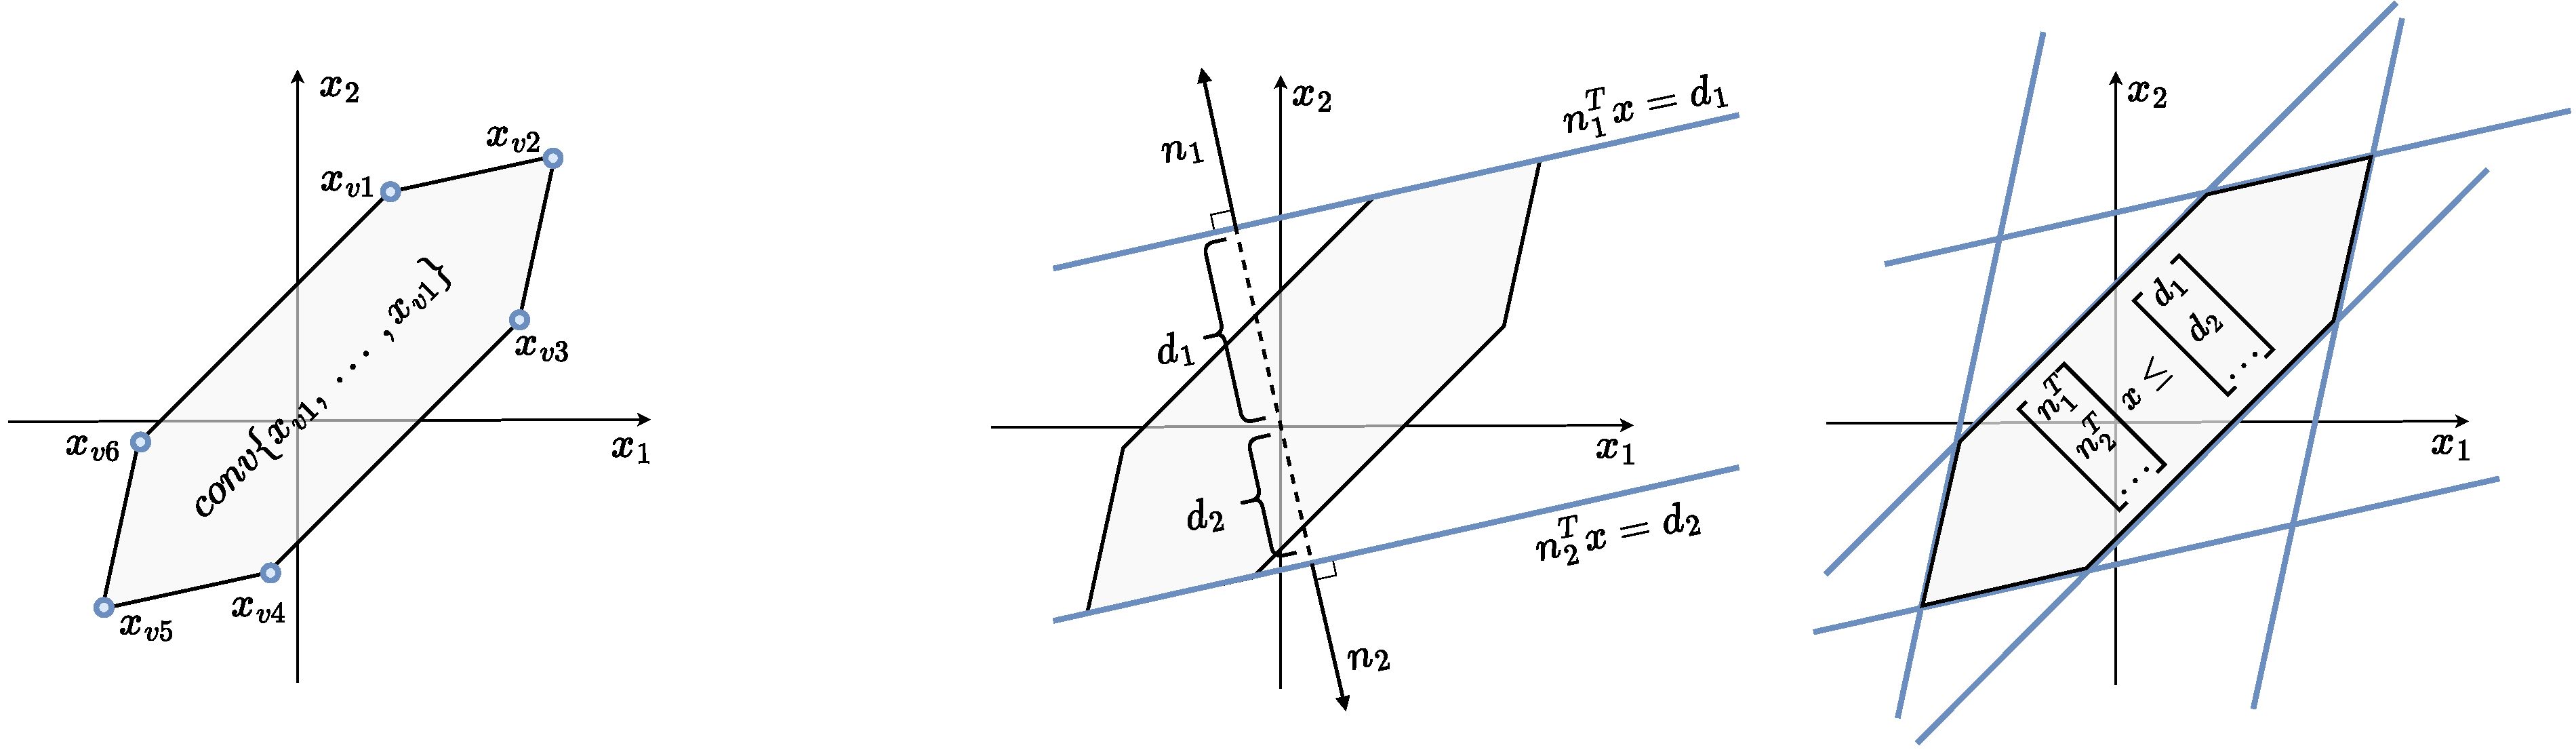
\includegraphics[width=\linewidth]{Chapters/imgs/h_v_rep.pdf}
    \caption{Figure illustrating the vertex ($\repr{V}$) and  half-plane ($\repr{H}$) representations of a polytope on a simple planar example. Image on the left shows the $\repr{V}$-representation as a Convex-Hull of the specified vertices. Images on the right show the $\repr{H}$-representation as an intersection of the half-planes (lines in 2D) representing the faces of the polytope $\mathcal{P}_x$.}
    \label{fig:hv_rep}
\end{figure}

Several alternative polytope representations were proposed recently, such as the $\repr{Z}$-representation \cite{kochdumper2019representation} where the polytopes are represented as polynomial zonotopes, and the $\repr{M}$-representation \cite{sigl2023mrepresentation} which is a more compact special case of the $\repr{Z}$-representation. These representations offer an improved efficiency of conducting polytope algebra operations, with respect to the traditional $\repr{H}$ and $\repr{V}$-representations. However, despite these advancements, their practical applications are still quite limited, primarily due to the challenging computational complexity involved in transforming polytopes into these alternative representations. 

Representing polytopes in these standard forms enables using different efficient tools from computational geometry and polytope algebra to perform operations over polytopes and provides tools for exploiting them in practical applications. However, in many cases polytope formulations do not correspond neither to the $\repr{V}$ nor $\repr{H}$-representation. As a result, many algorithms are developed in the literature transforming different polytope formulations into one of the two standard forms. The algorithms transforming the polytopes to the $\repr{V}$-representation are often called \textit{vertex enumeration} algorithms and to the $\repr{H}$-representation of are called \textit{facet enumeration} algorithms \cite{bremner_fukuda_marzetta_1998}. The appropriate choice of suitable polytope transformation algorithm, and its complexity, depends on various factors such as the polytope formulation, the desired polytope representation ($\repr{V}$ or $\repr{H}$), and potentially the time constraints for algorithm execution (online or offline). 

Therefore, \Cref{ch:generic_view} brings a structured overview of different polytopes, especially the ones occurring when characterising different physical abilities of humans and robots, and classifies them with respect to their formulation. \Cref{ch:polytope_algorithms} then exploits this classification to provide an overview of their applicable polytope transformation strategies and briefly discusses their efficiency.

\section{Generic view on physical ability polytope formulations}
\label{ch:generic_view}

This section aims to present a generic perspective on different families of polytope formulations commonly found when characterising the physical abilities of humans and robots. These polytopes are categorised based on their formulation to facilitate the choice of applicable algorithms.

From a generic standpoint, physical abilities represented in the shape of polytopes $\mathcal{P}_x$ can be seen as feasible sets of output (task space) variables $\bm{x} \in \mathbb{R}^m$, produced by applying a linear transformation on the input (actuation space) variables $\bm{y} \in \mathbb{R}^n$, bounded within (actuator limits) $\bm{y}\in\mathcal{P}_y$. As described in the previous chapter (\Cref{ch:collab_metrics_overview}), the polytope formulations for characterising physical abilities can be expressed in a unified generic form 
\begin{equation}
    \mathcal{P}_x = \{\bm{x}\in\mathbb{R}^m ~|~ A\bm{x}=B\bm{y} + \bm{b}, ~ \bm{y}\in\mathcal{P}_y\}
    \label{eq:generic_polyt_view_revisit}
\end{equation}
where matrices $B\in\mathbb{R}^{k\times n}$ and $A\in\mathbb{R}^{k\times m}$ present the linear transformation of the $n$ dimensional input to $m$ dimensional output space, through the $k$ dimensional intermediate space, while $\bm{b}\in\mathbb{R}^k$ is a bias vector. Furthermore, in the context of this work, the dimension of output space $m$ is considered to be lower or equal to the intermediate space dimension $k\!\geq\! m$ , which is in term lower or equal to the input space dimension $n\!\geq\! k\!\geq\! m$. In practice, this condition implies that the human or the robot model considered have at least the same number of degrees of freedom (DOF) as the dimension of the output space $m$. 

This compact and implicit formulation represents a unified view of different physical ability polytope formulations. However, depending on the structure of the matrices $A$ and $B$, as well as on the form of the input set $\mathcal{P}_y$, different algorithms are required to transform this formulation to its standard representations ($\repr{H}$ and $\repr{V}$). 

One important factor for determining the complexity of the polytope transformation, and the choice of the suitable algorithm, is the shape of the input set, corresponding to the limits of the input variable $\bm{y}\in\mathbb{R}^n$ limits. There are two most common forms that can be considered: interval form $\mathcal{I}_y$ and polytope form $\mathcal{P}_y$. 

The interval shaped $\mathcal{I}_y$ input set is specified in a form of min-max intervals
\begin{equation}
    \mathcal{I}_y = \{\bm{y}\in \mathbb{R}^n |~~ \bm{y}_{min} \leq \bm{y}\leq \bm{y}_{max} \}
    \label{eq:hypercube_lim}
\end{equation}
In a geometric sense, these individual intervals of the input variable $\bm{y}$ can be visualised as an $n$-dimensional hyperrectangle, also known as a hyperbox or an orthotope. Each axis $i$ of the hyperrectangle corresponds to an interval $y_i\in[y_{i,\text{min}},y_{i,\text{max}}]$.

More generally, rather than an interval $\mathcal{I}_y$, the input set can be defined as any convex polytope (ex. set of linear constraints in its $\repr{H}$-representation).
\begin{equation}
    \mathcal{P}_y = \{\bm{y}\in \mathbb{R}^n|~~ H_y\bm{y}\leq \bm{d}_y \}
\end{equation}

As polytopes $\mathcal{P}_x$ are then defined as linear transformations $A\bm{x}\!=\!B\bm{y}\! +\! \bm{b}$ of the input set (intervals $\mathcal{I}_y$ or polytope $\mathcal{P}_y$ shaped) from the input space to the output space, the structure of the linear transformation (matrices $A$ and $B$) has a direct impact on the complexity of the formulation, as well as on the choice of the algorithm.
Therefore, in this work, the distinction between two generic families of polytope formulations is proposed, derived from the unified formulation (\ref{eq:generic_polyt_view_revisit}): the projection formulation, where matrix $A$ is identity matrix $A=I_{m\times m}$, and the intersection formulation, where 
$B=I_{n\times n}$.

\subsection{Projection formulation}
\label{ch:proj_formulaiton}

\begin{figure}[!h]
    \centering
    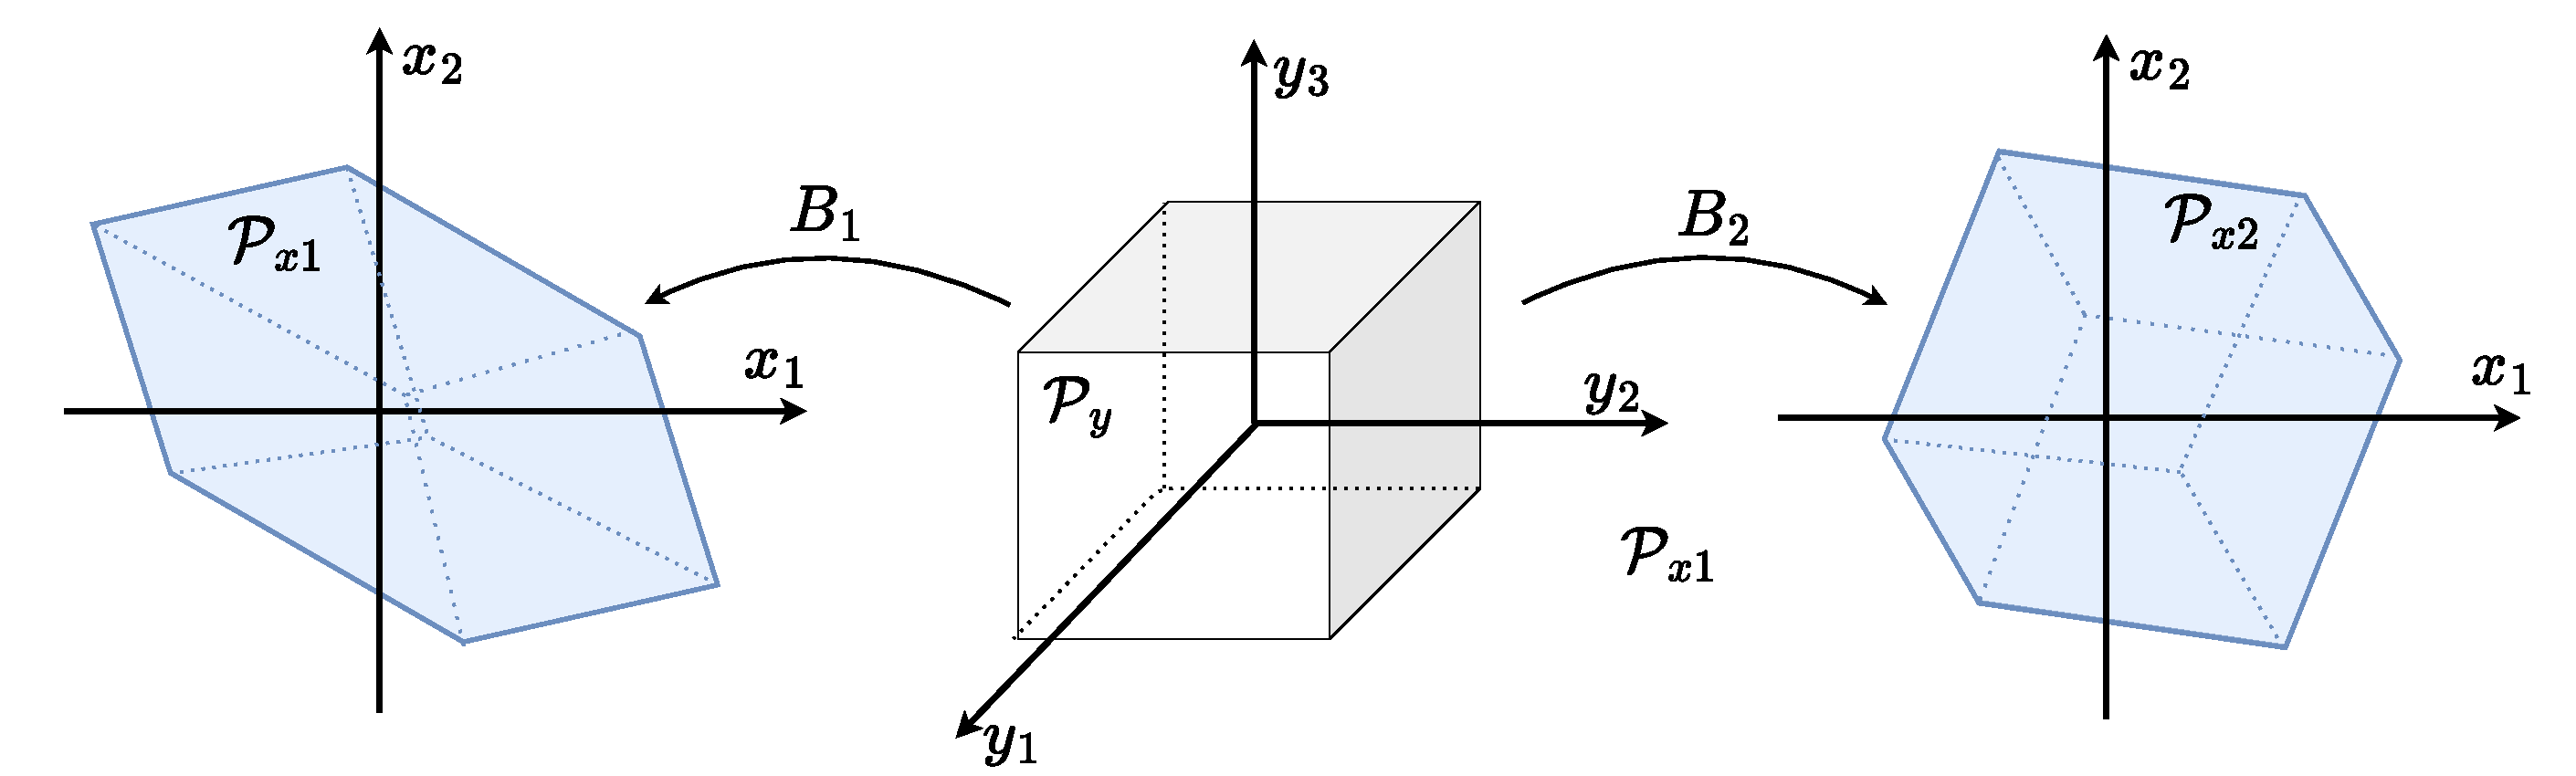
\includegraphics[width=0.8\linewidth]{Chapters/imgs/projection_double.pdf}
    \caption{An example ($m=2$, $n=3$) of constructing two different projection formulation polytopes, from the same input set $\mathcal{P}_y$. Polytopes $\mathcal{P}_{x1}$ and $\mathcal{P}_{x2}$ represent linear affine transformations of the input set $\mathcal{P}_y$ using two different transformation matrices $B_1$ and $B_2$.}
    \label{fig:proj_zono}
\end{figure}

The projection formulation is defined through a linear affine transformation of the $n$ dimensional input space $\bm{y}\in\mathbb{R}^n$ to the $m$ dimensional output space $\bm{x}\in\mathbb{R}^m$ using the projection matrix $B\in \mathbb{R}^{m\times n}$
\begin{equation}
    \mathcal{P}_x=\{\bm{x}\in \mathbb{R}^m ~|~ \bm{x} = B\bm{y} + \bm{b}_x,~\bm{y} \in\mathcal{P}_y \}
    \label{eq:proj_poly}
\end{equation}
where $\bm{b}_x\in\mathbb{R}^m$ is a constant bias vector, defined in the output space. The name \textit{projection} formulation comes from the fact that the polytope $\mathcal{P}_x$, in this formulation, is a projection of the $n$ dimensional input set $\mathcal{P}_y$ to the $m$ dimensional output space $\mathbb{R}^m$ \cite{Burger1996projection}.

A graphical representation of the projection formulation (\ref{eq:proj_poly}) is shown on \Cref{fig:image_projection_two}, where two different output polytopes $\mathcal{P}_x$ are constructed applying different affine transformation matrices $B$ on the same input set $\mathcal{P}_y$.


\subsubsection*{Zonotope formulation} If the input space has the interval shape $\mathcal{I}_y$, the final polytope $\mathcal{P}_x$, defined by the equation (\ref{eq:proj_poly}), has a zonotope form. In that case the polytope $\mathcal{P}_x$ can be represented as a Minkowski sum of $n$ line segments $\mathcal{L}_i$, each one corresponding to one axis range $[y_{i,min}, y_{i,max}]$ of the input set $\mathcal{I}_y$ projected to the output space using the matrix $B$.  \cite{McMullen1971onzonotopes}
\begin{equation}
    \mathcal{P}_x = \mathcal{L}_1 \oplus~ \cdots ~\oplus \mathcal{L}_n
\end{equation}
where the $i$-th line segment $\mathcal{L}_i$ can be expressed through $i$-th line vector $\bm{b}_i$ of the matrix $B$
\begin{equation}
    \mathcal{L}_i = \{\bm{x}\in\mathbb{R}^m ~|~ \bm{x} = \bm{b}_iy_i + \bm{b}_x,~~ y_i\in [y_{i,min}, y_{i,max}] \}
\end{equation}
\begin{wrapfigure}{r}{0.5\linewidth}
\vspace{-0.5cm}
% \begin{framed}
    \centering
    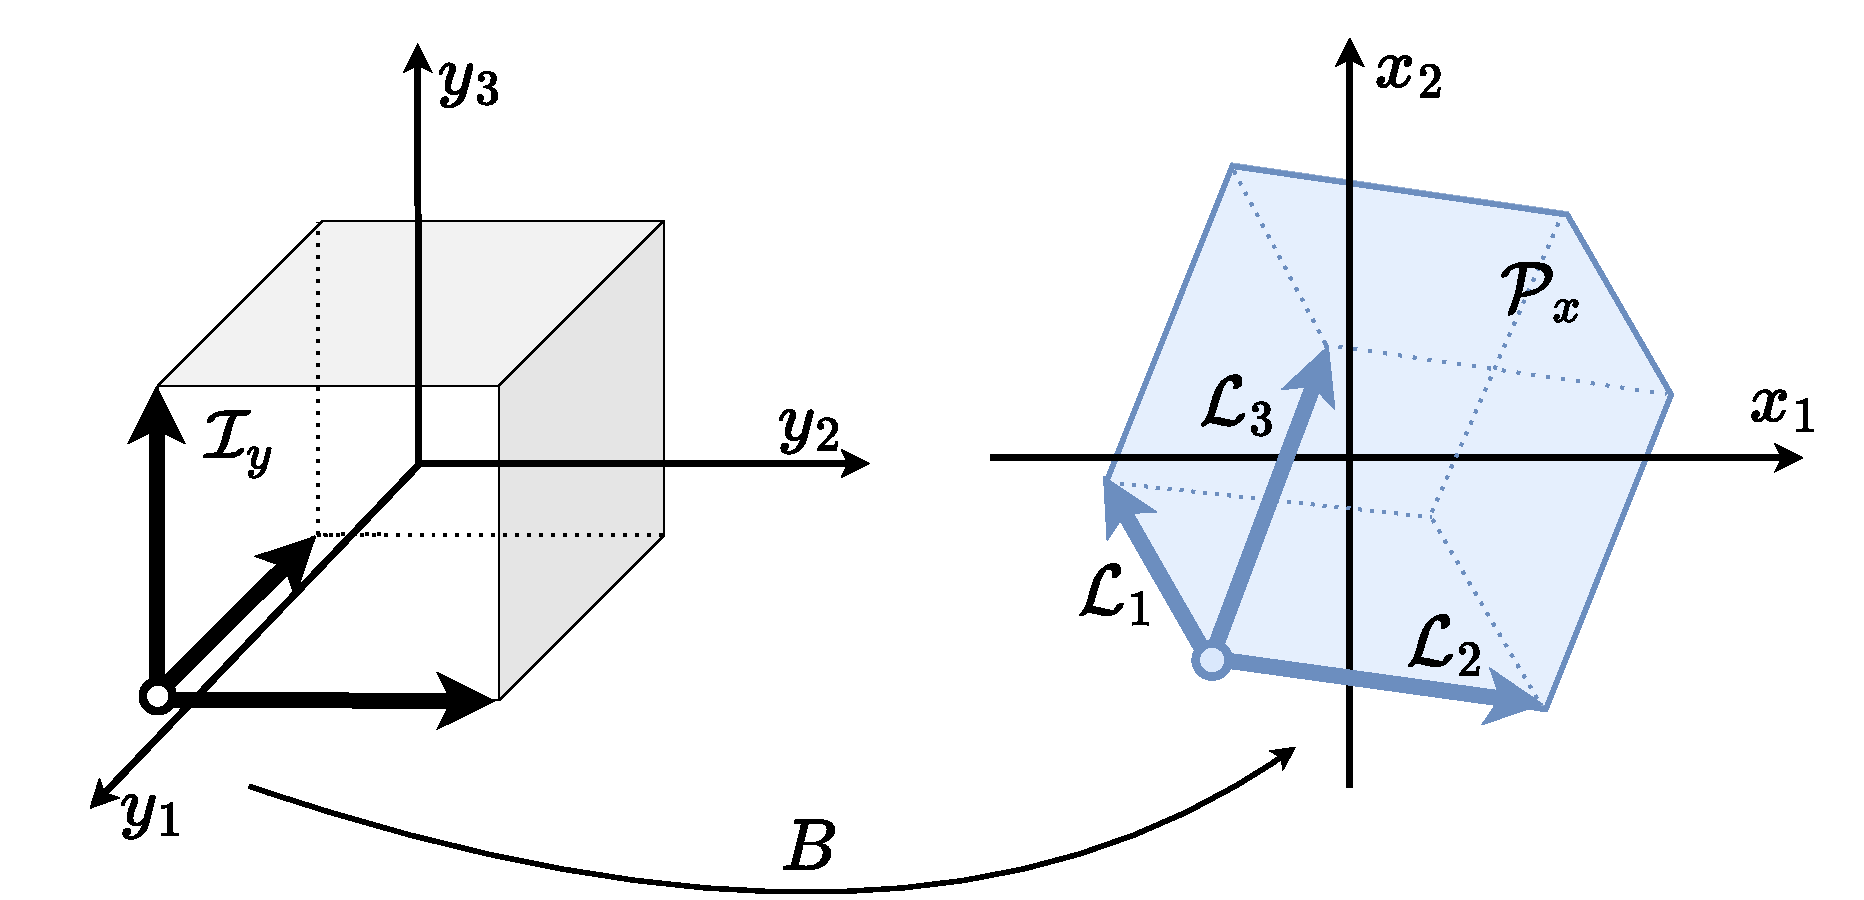
\includegraphics[width=\linewidth]{Chapters/imgs/zonotope_only.pdf}
    \caption{A graphical example ($m=2$, $n=3$) of constructing the zonotope shaped polytope $\mathcal{P}_x$ from the interval input set $\mathcal{I}_y$.}
    \label{fig:image_projection_two}
% \end{framed}
\end{wrapfigure}
These line segments are often called \textit{components} or \textit{generators} of the zonotope $\mathcal{P}_x$ \cite{shephard1974zonotopes}.

More generally, for any zonotope shaped input set $\mathcal{P}_y$, expressed as a Minkowski sum of the generators $\mathcal{L}_{yi}$
\begin{equation}
    \mathcal{P}_y = \mathcal{L}_{y1}  ~\oplus \mathcal{L}_{y2}~\oplus~ \cdots
\end{equation}
polytope $\mathcal{P}_x$ is a zonotope as well. The generators $\mathcal{L}_i$ of the polytope $\mathcal{P}_x$ correspond to the generators $\mathcal{L}_{yi}$ of the input set $\mathcal{P}_y$, projected to the output space using the equation (\ref{eq:proj_poly}). Therefore, polytope $\mathcal{P}_x$ has the same number of generators $\mathcal{L}_i$ as the zonotope $\mathcal{P}_y$, which can be expressed as
\begin{equation}
    \mathcal{L}_i = \{\bm{x}\in\mathbb{R}^m ~|~ \bm{x} = B\bm{y} + \bm{b}_x,~~ \bm{y}\in  \mathcal{L}_{yi}\}
\end{equation}

Zonotopes are highly structured and central symmetric shapes, hence transforming them to appropriate representations ($\repr{H}$ and $\repr{V}$) is in many cases more efficient than for generic polytopes.


\subsection{Intersection formulation}
\label{ch:inter_formulaiton}

\begin{figure}[!h]
    \centering
    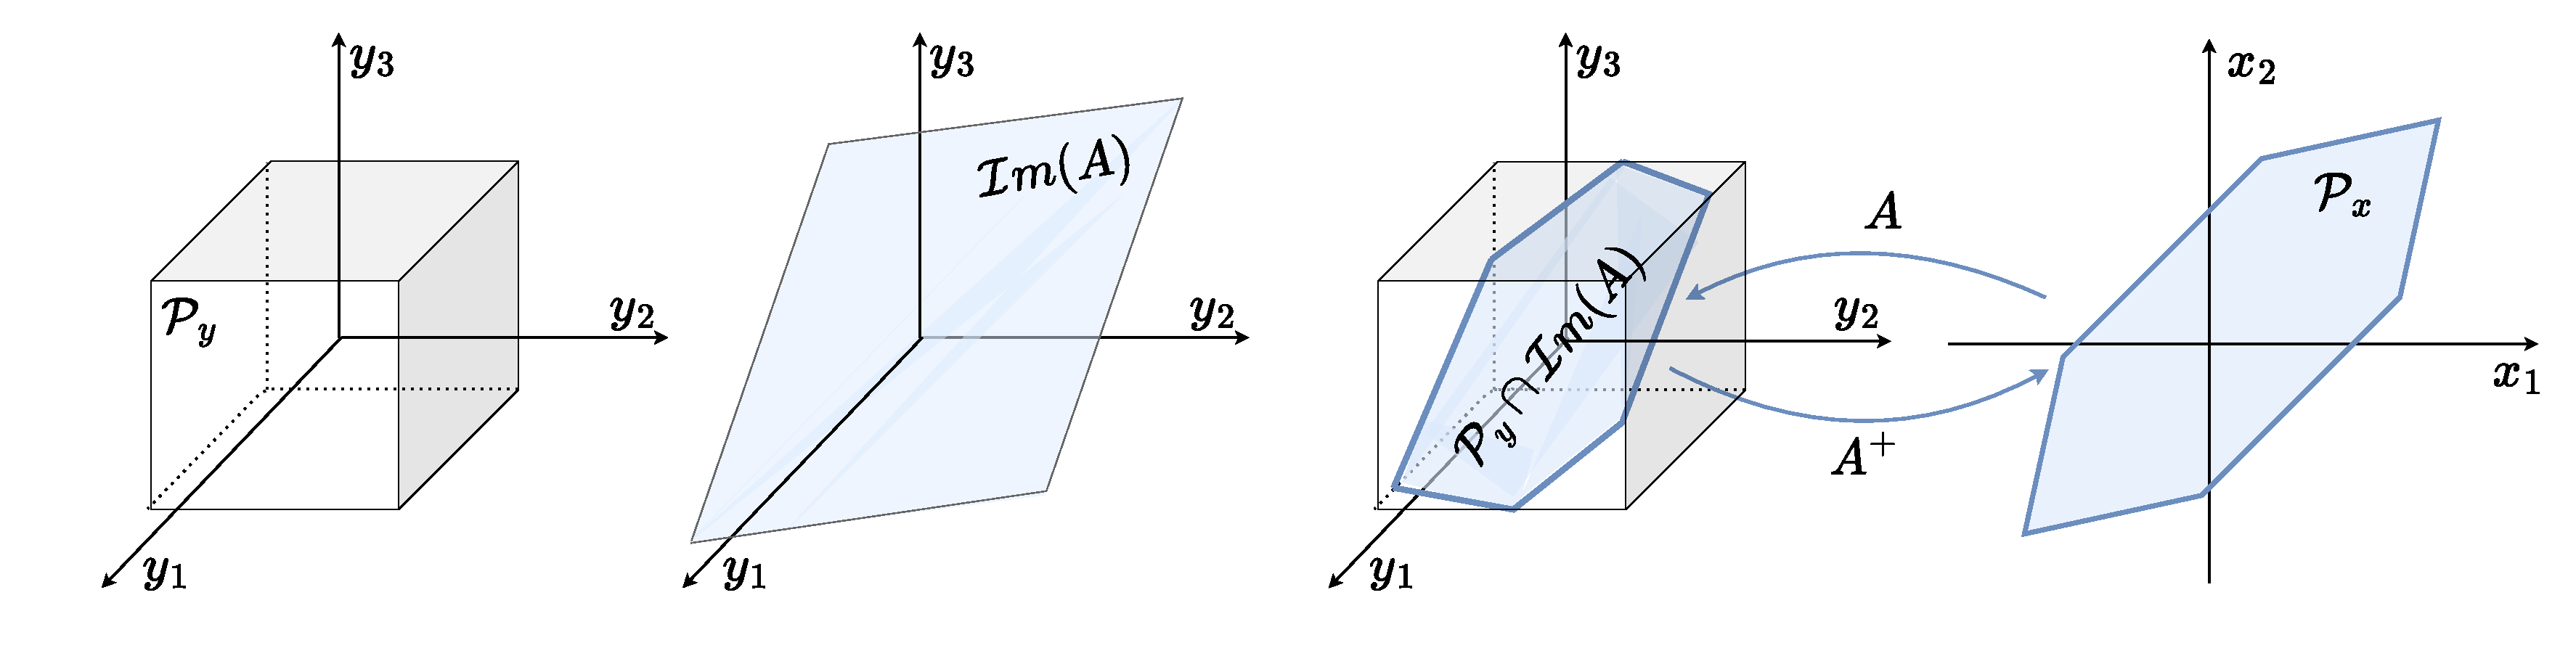
\includegraphics[width=\linewidth]{Chapters/imgs/image_intersection_poly_all.pdf}
    \caption{An example ($m=2$, $n=3$) of constructing a intersection formulation polytope $\mathcal{P}_x$ from the input set $\mathcal{P}_y$. First the image $\img{A}$ of the matrix $A$ is intersected with the input set $\mathcal{P}_y$, then this intersection is projected to the output space using the pseudo-inverse $A^+$. }
    \label{fig:inter_image_poly}
\end{figure}
The intersection formulation, on the other hand, is expressed by a matrix equation $A\bm{x}=\bm{y}$. It can be interpreted as a linear transformation in the opposite direction \cite{LARSON2013}, from the $m$ dimensional input space $\bm{x}\in\mathbb{R}^m$ to the $n$ dimensional output space $\bm{y}\in\mathbb{R}^n$, using the projection matrix $A\in \mathbb{R}^{n\times m }$
\begin{equation}
    \mathcal{P}_x=\{\bm{x} \in \mathbb{R}^m|~ A\bm{x} = \bm{y}+ \bm{b}_y,~ \bm{y} \in \mathcal{P}_y\}
    \label{eq:inter_poly}
\end{equation}
where $\bm{b}_y \in \mathbb{R}^n$ is a constant bias vector, defined in the input space. The name \textit{intersection} formulation comes from the fact that the polytope $\mathcal{P}_x$ is no longer just a projection of the input set $\mathcal{P}_y$ to the $m$ dimensional output space, but rather a projection of its intersection with the image $\img{A}$ of matrix $A$. 
A graphical representation of the intersection formulation (\ref{eq:inter_poly}) is shown on \Cref{fig:inter_image_poly}, where the intersection $\mathcal{P}_y\cap \img{A}$ and the final polytope $\mathcal{P}_x$ are denoted in blue.

The main difficulty of the intersection formulation (\ref{eq:inter_poly}) is that it is defined as an inverse projection, from the $m$ dimensional output space to the $n$ dimensional input space \cite{LARSON2013}. In order to inverse this relationship, an equivalent projection formulation polytope can be constructed by characterising the intersection $\mathcal{P}_y\cap \img{A}$. 

\subsubsection*{Equivalent projection formulation}\label{par:equivalent_proj} In order to express the intersection formulation in the projection form, it is necessary to inverse the relationship $\bm{y}=A\bm{x}$, considering $\bm{b}_y=\bm{0}$. If the input and output space have the same dimension $n=m$, $A$ is invertible and the inverse relationship can be easily obtained as $\bm{x} = A^{-1}\bm{y}$. 

\begin{wrapfigure}{r}{0.45\linewidth}
\vspace{-0.5cm}
% \begin{framed}
    \centering
    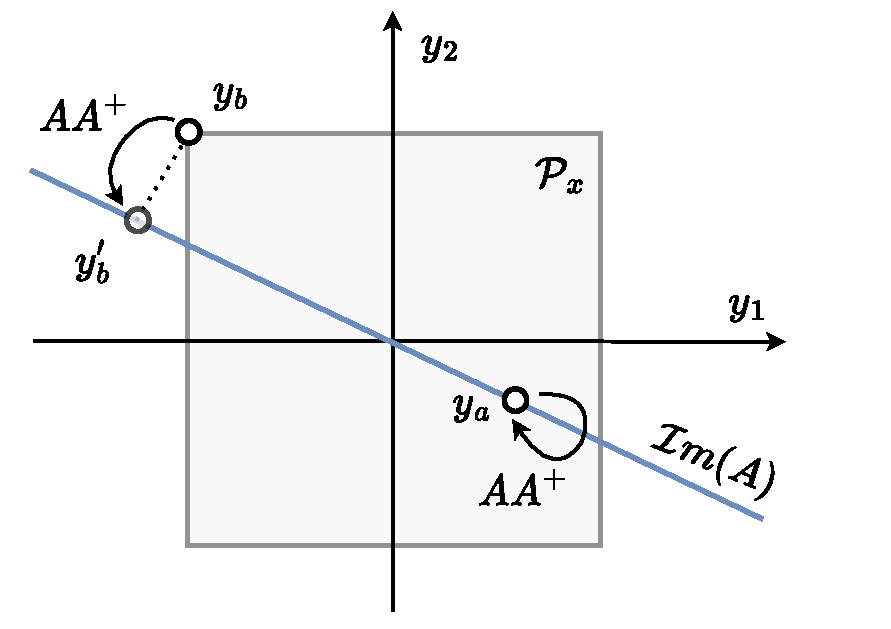
\includegraphics[width=\linewidth]{Chapters/imgs/img_pseudo_prob.pdf}
    \caption{An example ($n=2$,$m=1$) of applying the image projector $AA^+$ in the input space, the input set $\mathcal{P}_y$ is shown in grey and the image $\img{A}$ in blue. As the input vector $\bm{y}_a$ belongs to the image $\img{A}$ its multiplication with $AA^+$ results in the same vector. $\bm{y}_b$  does not belong to the image and $AA^+$ results in $\bm{y}_b'$, its orthogonal projection onto the image $\img{A}$ is outside the input set $\mathcal{P}_y$.}
    \label{fig:image_psueodinverse_ilustration}
% \end{framed}
\end{wrapfigure}

However, in the more general case, the input space is higher dimensional $n>m$, making  matrix $A$ not invertible. In such cases the inverse relationship can be obtained using the left pseudo-inverse of matrix $A$
\begin{equation}
    \bm{x} = (A^TA)^{-1}A^T\bm{y} = A^+\bm{y}
    \label{eq:pseudoinverse_equation}
\end{equation}

Due to the fact that, in the general case, the operation $\bm{x}\!=\!A^+\bm{y}$ is not bijective, the input vector $\bm{y}'\!=\!A\bm{x}$ corresponding to the output vector $\bm{x}\!=\!A^+\bm{y}$ does not correspond to the original input vector $\bm{y}$ 
\begin{equation}
\bm{y}' = A\bm{x} = A(A^+\bm{y})\neq\bm{y}
\end{equation}
making it possible that the input vector ${\bm{y}'\!=\!AA^+\bm{y}}$ no longer respects the input set $\mathcal{P}_y$
\begin{equation}
    \bm{y}'=AA^+\bm{y}\notin\mathcal{P}_y
\end{equation}

The matrix $AA^+$ represents an orthogonal projector matrix to the \textit{image space} $\img{A}$ of the matrix $A$ \cite[Chapter 5.5.4]{golub1996matrix}. Therefore, for any input vector $\bm{y}$ belonging to the image $\img{A}$, the multiplication by $AA^+$ results in itself \cite[Chapeter 1.3.1]{wang2018generalized}
\begin{equation}
    \bm{y} = AA^+\bm{y}, \qquad \forall \bm{y}\in\img{A}
    \label{eq:image_projector}
\end{equation}
However, for any input vector $\bm{y}$ not belonging to the image $\img{A}$, multiplying it with the matrix $AA^+$ will result in its orthogonal projection to the image $\img{A}$. As shown in the graphical example on \Cref{fig:image_psueodinverse_ilustration}, even though the original $\bm{y}$ respects the input set $\mathcal{P}_y$, its orthogonal projection onto the image $AA^+\bm{y}$ does not is some cases.

Therefore, having ensured that all the inputs $\bm{y}$ belong to the image $\img{A}$, the pseudo-inverse $A^+$ provides a unique inverse solution to the equation $\bm{y} = A\bm{x}$. Then, the new input set, respecting the limitations $\bm{y}\in\mathcal{P}_y$ and ensuring the unique inverse solution, can be found as the intersection
\begin{equation}
   \bm{y} \in \img{A} \cap \mathcal{P}_y
    \label{eq:intersection_ai}
\end{equation}
By exploiting the new input set and using the pseudo-inverse $A^+$, the equivalent formulation of the the initial intersection polytope $\mathcal{P}_x$ can be expressed as
\begin{equation}
\mathcal{P}_x=\{\bm{x}\in\mathbb{R}^m~|~ \bm{x} = A^+\bm{y} + A^+\bm{b}_y,~ \bm{y} \in \img{A}\cap\mathcal{P}_y\} \label{eq:proj_inter}
\end{equation}

Using the formulation (\ref{eq:proj_inter}), in practice, often requires characterising the image $\bm{y}\in\img{A}$ in a set form as well. As shown in expression (\ref{eq:image_projector}), all the vectors $\bm{y}$ belonging to the image $\img{A}$, when multiplied with the image projector $AA^+$ result in themselves ($\bm{y} - AA^+\bm{y} = \bm{0}$). This relationship can be exploited to formulate a compact set form of the image $\img{A}$ 
\begin{equation}
   \img{A} = \{ \bm{y}\in\mathbb{R}^n ~|~(I_{n\times n} - AA^+)\bm{y} = \bm{0}, \quad \bm{y}\in\mathbb{R}^n \}
   \label{eq:image_poly}
\end{equation}

\Cref{fig:inter_image_poly} provides a graphical representation of the mapping (\ref{eq:proj_inter}), showing the intersection $\img{A}\cap\mathcal{P}_y$ and the final polytope $\mathcal{P}_x$, being its projection to the output space $\bm{x}\in \mathbb{R}^m$. 

The intersection formulation is generally more computationally complex to work with than the projection formulation, as it often requires characterising the intersection $\img{A}\cap\mathcal{P}_y$. The graphical comparison of the construction of both intersection and projection polytopes from the same input set is shown on \Cref{fig:inter_proj}.


\begin{figure}
    \centering
    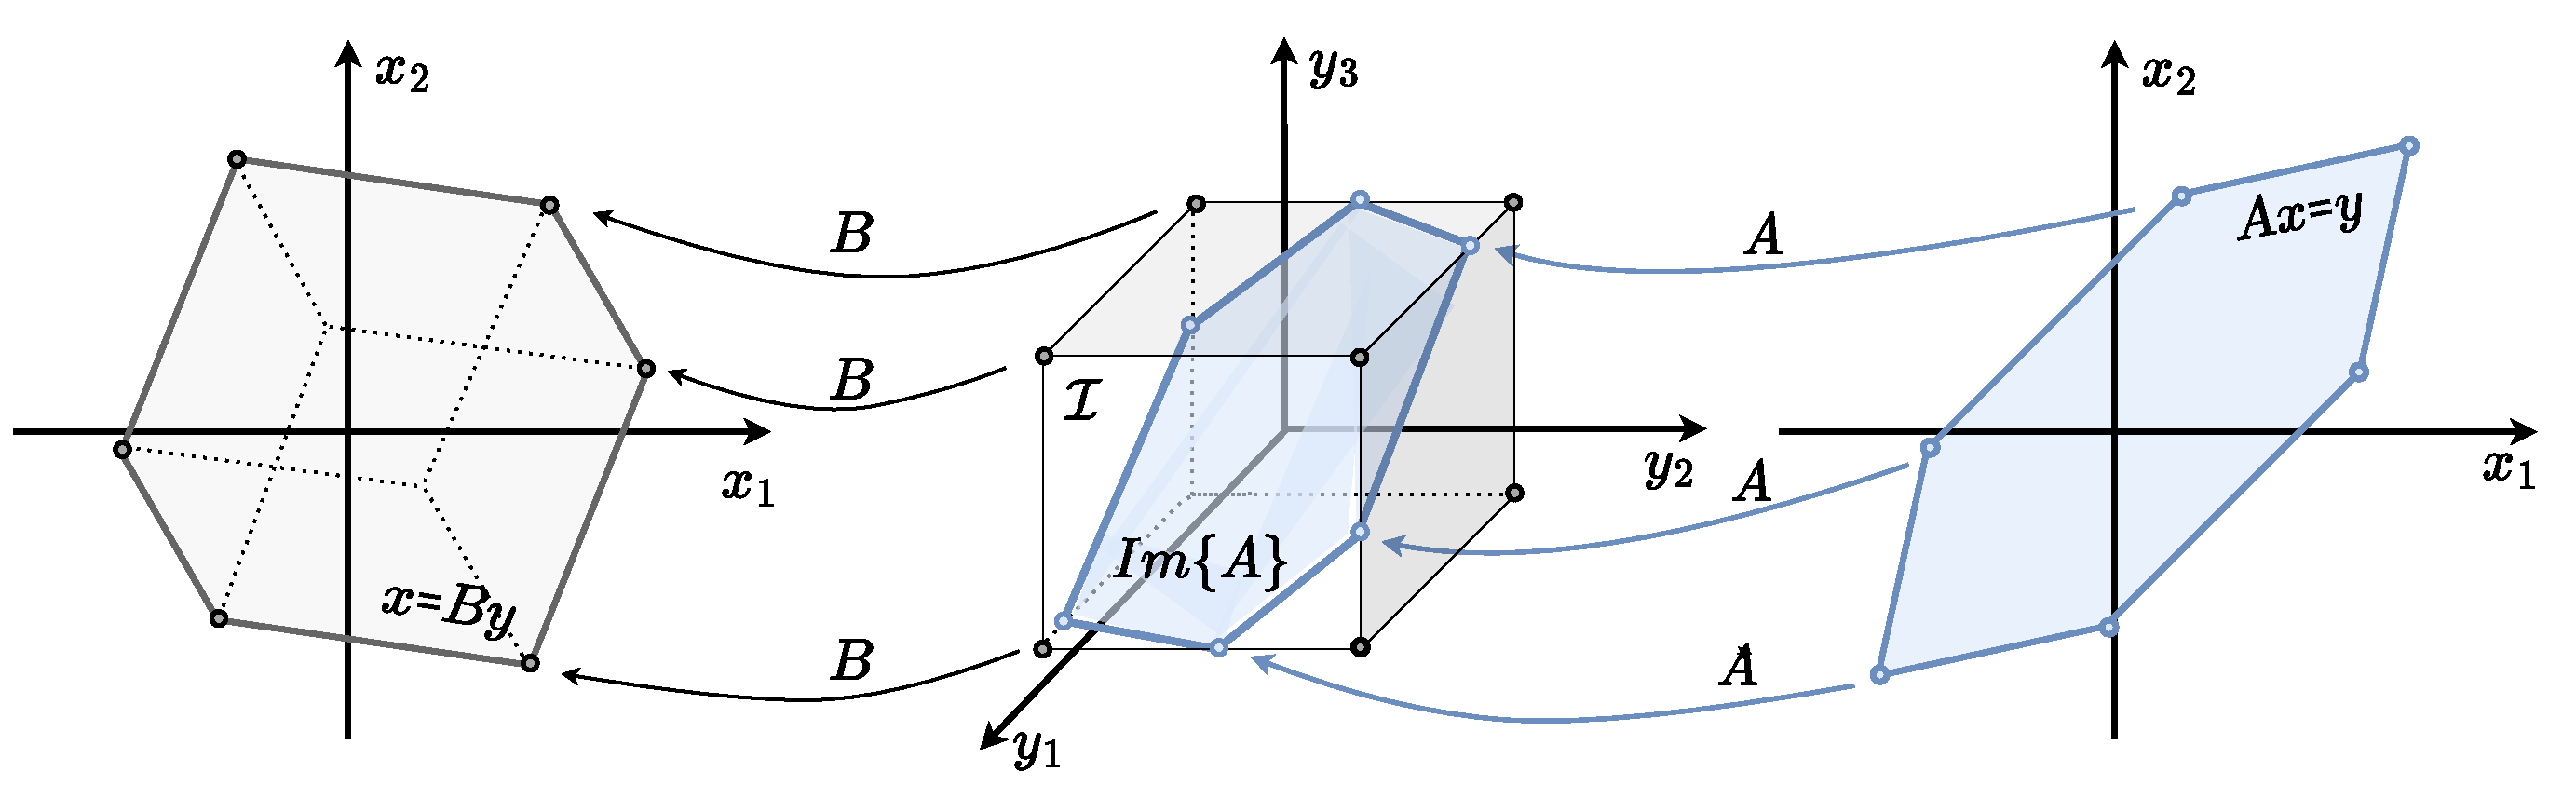
\includegraphics[width=\linewidth]{Chapters/imgs/intersection_projection.pdf}
    \caption{A comparative view of the projection (left) and intersection (right) polytope formulation using the same input space (middle). In the projection formulation, the whole input space $\mathcal{P}_y$ is projected using the matrix $B$ to the output space to obtain the polytope $\mathcal{P}_x$ (grey left). In the intersection formulation, first the intersection of the input space $\mathcal{P}_y$ with the image of the matrix $A$ is found (blue middle) $\img{A} \cap \mathcal{P}_y$, then this intersection can be projected to the output space using the pseudo-inverse $A^+$ of the matrix $A$ to obtain the polytope $\mathcal{P}_x$ (blue right).}
    \label{fig:inter_proj}
\end{figure}

\subsection{Combined cases}
\label{ch:combined_forms}
Physical ability polytopes described in \Cref{ch:human_metrics} contain two special cases consisting in the combination of intersection and projection polytope formulations: \textit{intersection-projection} and \textit{projection-intersection} formulation.

\subsubsection{Intersection-projection formulation}
\label{ch:inter_proj_form}

The unified generic polytope formulation given by the equation (\ref{eq:generic_polyt_view_revisit}) can be seen as a special case of the polytope formulation that contains both intersection and projection formulation
\begin{equation}
    \mathcal{P}_x \in \{\bm{x}\in \mathbb{R}^m~|~\underbrace{A \bm{x}= \bm{z}+ \bm{b}_z}_{\text{intersection}},~ \underbrace{ \bm{z}=B \bm{y}}_{\text{projection}} ,~ \bm{y} \in \mathcal{P}_y\} 
    \label{eq:inter_proj_poly}
\end{equation}
where $\bm{x}\in\mathbb{R}^m$ is the output vector, $\bm{y} \in \mathbb{R}^n$ is an input vector and $\bm{z}\in\mathbb{R}^k$ is an intermediate space vector, where $n\!\geq\!k\!\geq\!m$. Matrix $B\in \mathbb{R}^{k \times n}$ is a projector matrix from $n$ dimensional input space to the $k$ dimensional intermediate space, matrix $A\in \mathbb{R}^{k\times m}$ is a projector matrix from $m$ dimensional output space to the $k$ dimensional intermediate space and $\bm{b}_z\in\mathbb{R}^k$ is the bias vector, defined in the intermediate space.

In this work, this polytope formulation is named \textit{intersection-projection} as it is a special case of a intersection formulation (\ref{eq:inter_poly}) with polytope shaped input set which has the projection formulation. The final polytope $\mathcal{P}_x$ can be expressed as
\begin{equation}
    \mathcal{P}_x \in \{\bm{x}\in \mathbb{R}^m~|~A \bm{x} = \bm{z} + \bm{b}_z,~ \bm{z} \in \mathcal{P}_z\} 
\end{equation}
where its input set polytope $\mathcal{P}_z$ is defined using the projection formulation
\begin{equation}
    \mathcal{P}_z \in \{\bm{z}\in \mathbb{R}^k~|~z = B\bm{y},~ \bm{y} \in \mathcal{P}_y\} 
\end{equation}

\begin{figure}[!t]
    \centering
    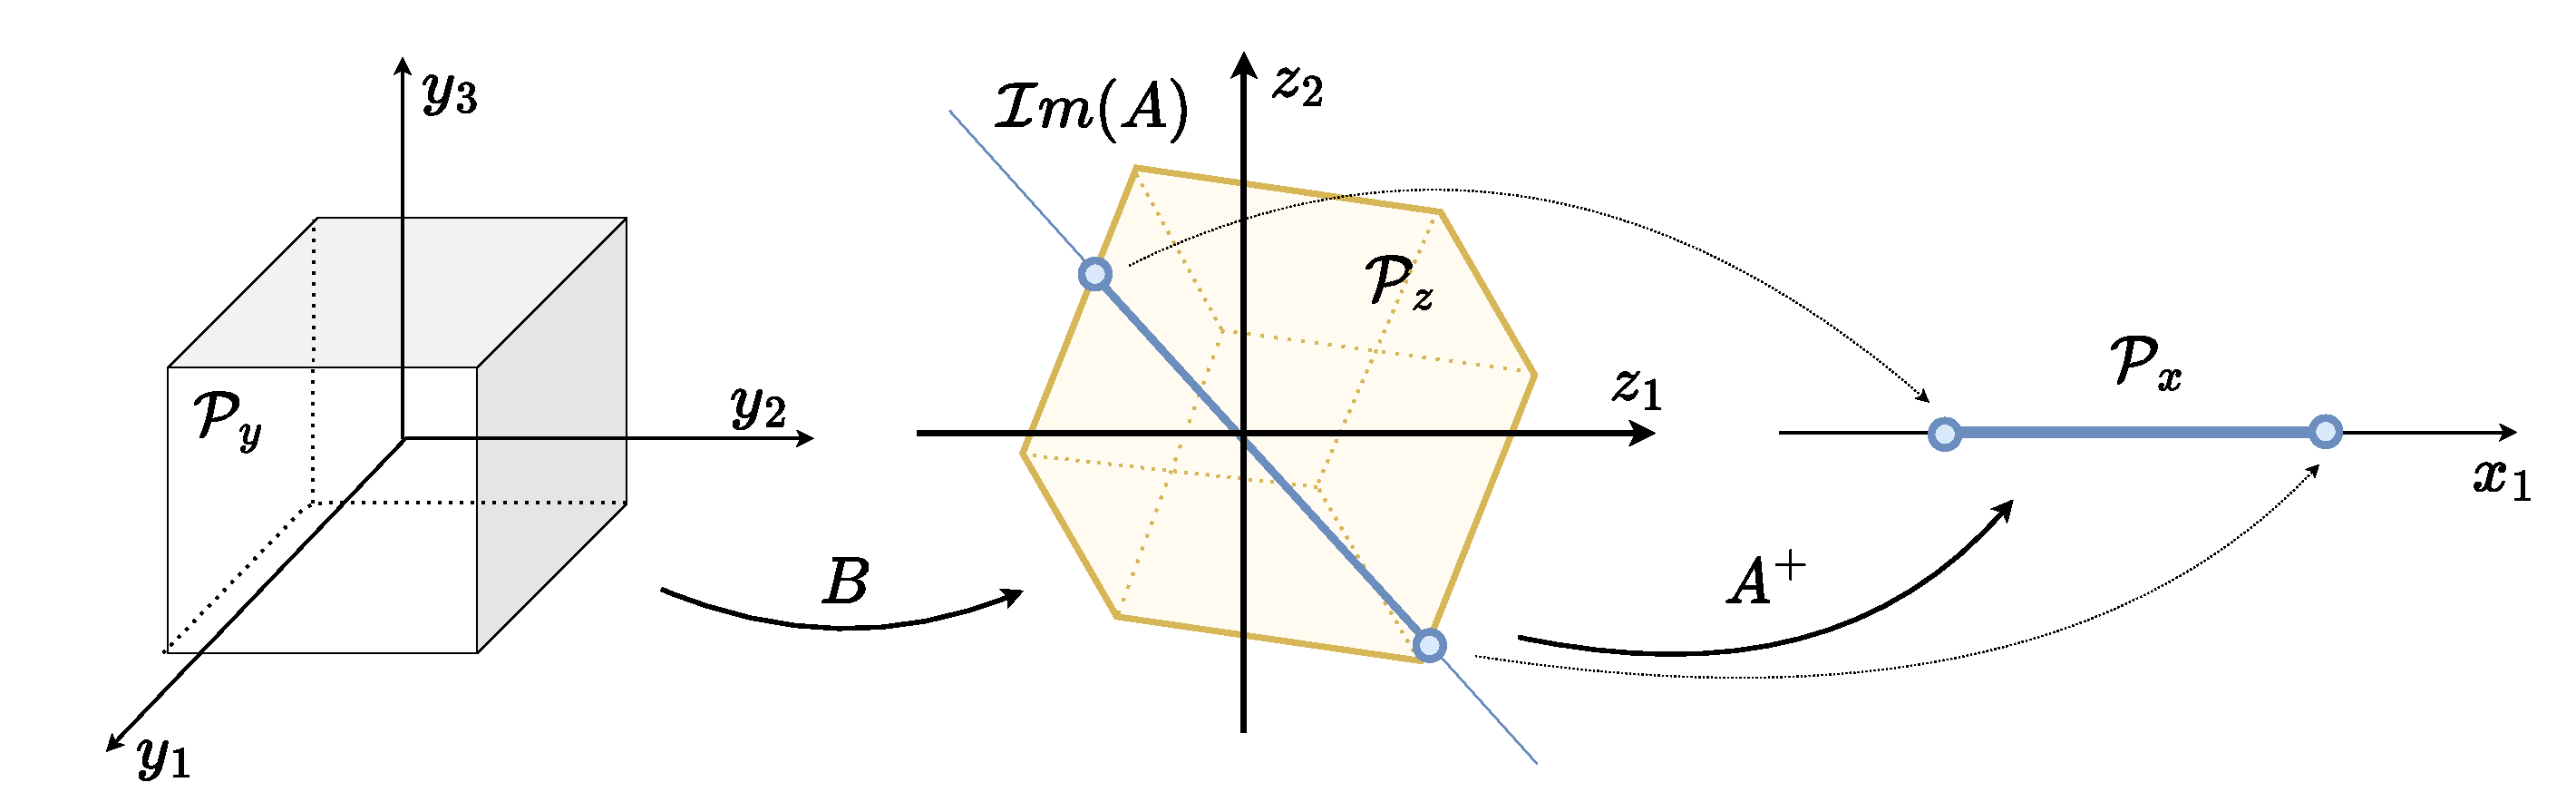
\includegraphics[width=\linewidth]{Chapters/imgs/spec_int_proj.pdf}
    \caption{An example ($n=3$, $k=2$, $m=1$) of a construction of the intersection-projection polytope $\mathcal{P}_x$ from the input set $\mathcal{P}_y$. Geometrically, first the input set $\mathcal{P}_y$ is projected to the intermediate space $\mathbb{R}^k$ to obtain the projection polytope $\mathcal{P}_z$ (yellow). Then this polytope is intersected with the image $\img{A}$ of matrix $A$ (blue middle). Finally the intersection $\mathcal{P}_z\cap\img{A}$ is projected to the output space with the pseudo-inverse $A^+$ to obtain the final 1D polytope $\mathcal{P}_x$ (blue right).}
    \label{fig:inter_proj_spec}
\end{figure}
This formulation can also be transformed to an equivalent projection formulation, as described for the intersection formulation is \Cref{par:equivalent_proj}, resulting in a polytope 
\begin{equation}
\mathcal{P}_x=\{\bm{x} \in \mathbb{R}^m |~ \bm{x} = A^+\bm{z} - A^+\bm{b}_z,~ \bm{z}+\bm{b}_z \in \img{A}\cap\mathcal{P}_z\} 
\end{equation}

However, this polytope formulation is much more computationally complex than both intersection and projection formulation, as it requires first computing the projection polytope $\mathcal{P}_z$ and then finding the intersection $\img{A}\cap\mathcal{P}_z$ in order to find the polytope $\mathcal{P}_x$. A graphical example of constructing the intersection-projection formulation polytope is shown on \Cref{fig:inter_proj_spec}.


\begin{remark}
    This formulation corresponds to the formulations of the wrench and stiffness capacity polytopes for human musculoskeletal models, described in \Cref{ch:force_poly_human} and \Cref{ch:human_stiffness_poly}.
\end{remark}


\subsubsection{Projection-intersection formulation}
\label{ch:proj_inter_form}

\begin{figure}
    \centering
    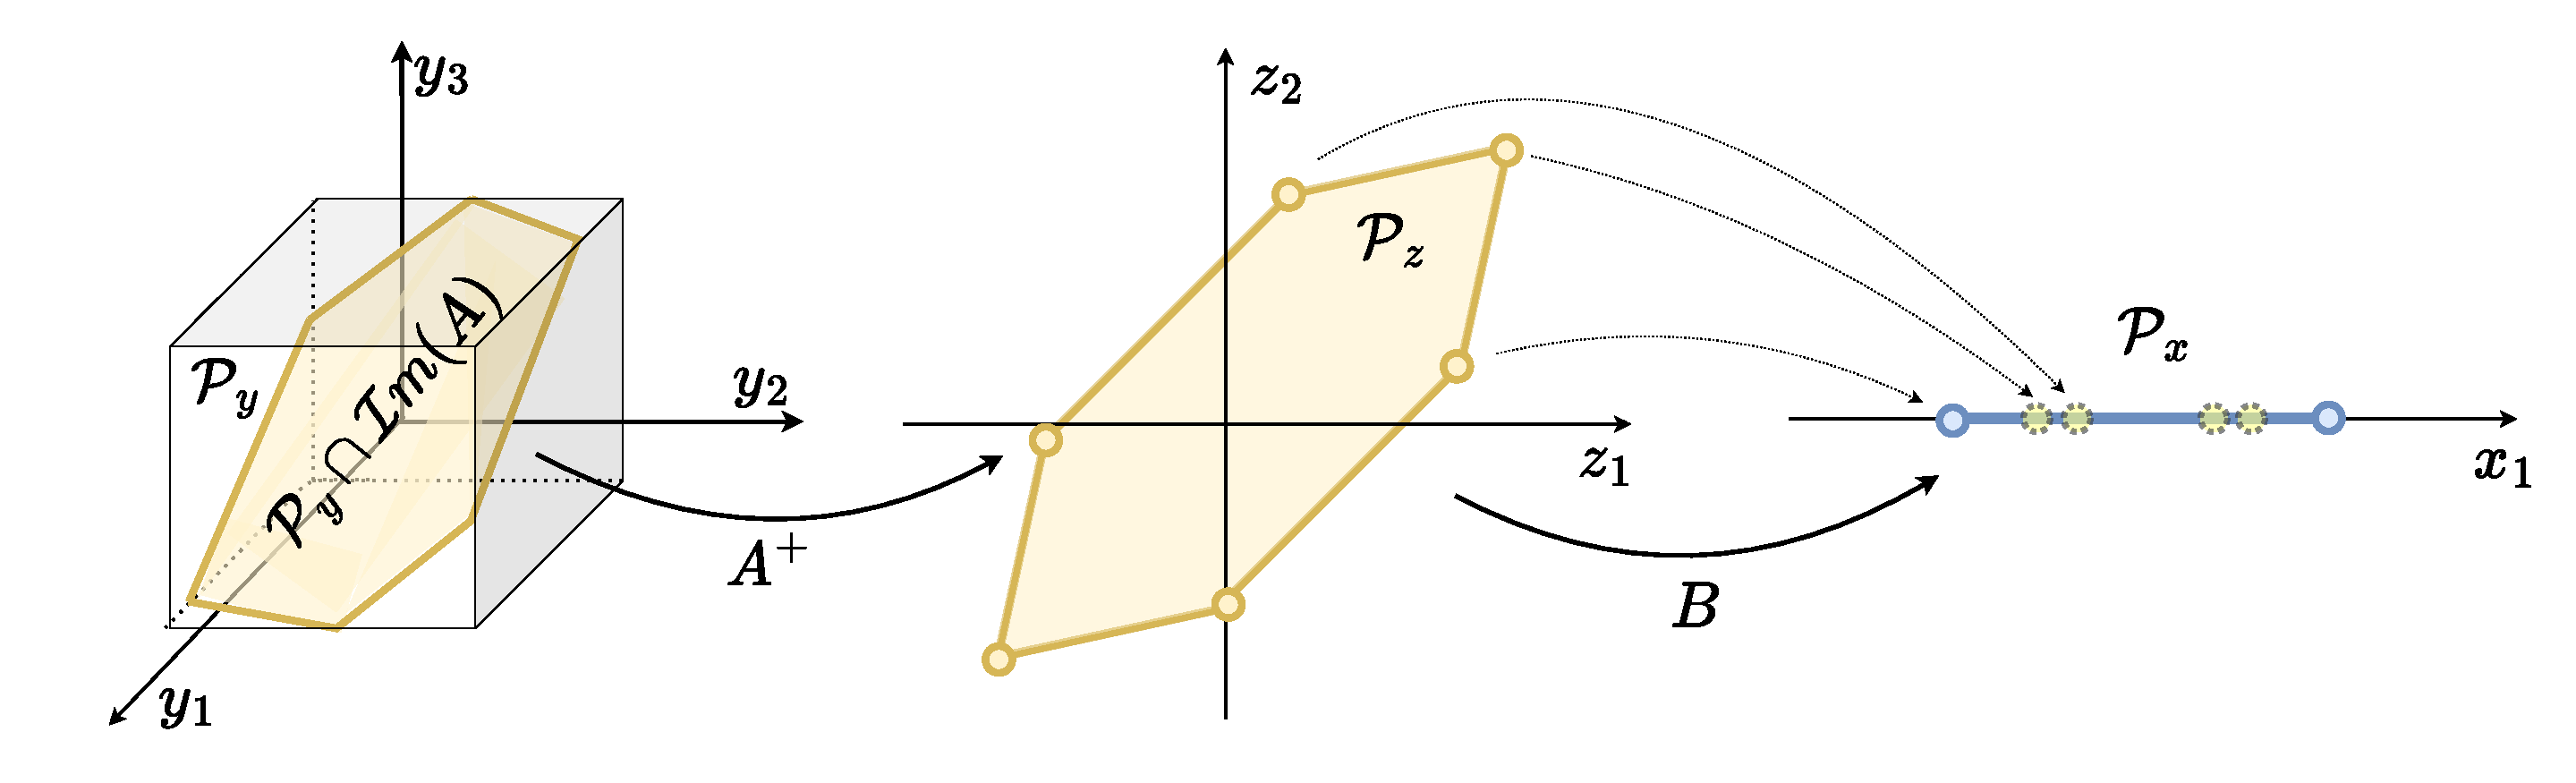
\includegraphics[width=\linewidth]{Chapters/imgs/spec_proj_int.pdf}
    \caption{An example ($n=3$, $k=2$, $m=1$) of a construction of the projection-intersection polytope $\mathcal{P}_x$ from the input set $\mathcal{P}_y$. 
    Geometrically, first the input set $\mathcal{P}_y$ is intersected with the image $\img{A}$ of the matrix $A$ (yellow left). The intersection $\mathcal{P}_y\cap\img{A}$ is then projected to the intermediate space using the pseudo-inverse $A^+$ to obtain the polytope $\mathcal{P}_z$ (yellow middle). Finally, an affine transformation $B$ is applied to the polytope $\mathcal{P}_z$ to transforming it to the final polytope 1D ($m=1$) $\mathcal{P}_x$ (blue right).}
    \label{fig:proj_inter_spec}
\end{figure}
A different special case of polytope formulation combining both projection and intersection formulation can be expressed as 
\begin{equation}
    \mathcal{P}_x \in \{\bm{x}\in \mathbb{R}^m~|~ \underbrace{\bm{x} = B \bm{z} + \bm{b}_x}_{\text{projection}},~ \underbrace{A\bm{z}=\bm{y}}_{\text{intersection}},~ \bm{y} \in \mathcal{P}_y\} 
    \label{eq:proj_inter_poly}
\end{equation}
where $\bm{x}\in\mathbb{R}^m$ is the output vector, $\bm{y} \in \mathbb{R}^n$ is an input vector and $\bm{z}\in\mathbb{R}^k$ is an intermediate space vector, where $n\!\geq\!k\!\geq\!m$. Matrix $A\in \mathbb{R}^{n\times k}$ is a projector matrix from $n$ dimensional input space to the $k$ dimensional intermediate space, matrix $B\in \mathbb{R}^{m\times k}$ is a projector matrix from $k$ dimensional intermediate space to the $m$ dimensional output space and $\bm{b}_x\in\mathbb{R}^m$ is the bias vector, defined in the output space.

In this work, this polytope formulation is named \textit{projection-intersection} as it is a special case of a projection formulation (\ref{eq:proj_poly}) with polytope shaped input set which has the intersection formulation. The final polytope $\mathcal{P}_x$ can be expressed as
\begin{equation}
    \mathcal{P}_x \in \{\bm{x}\in \mathbb{R}^m~|~ \bm{x} = B\bm{z} + \bm{b}_x,~ \bm{z} \in \mathcal{P}_z\} 
\end{equation}
where its input set polytope $\mathcal{P}_z$ is defined using the intersection formulation
\begin{equation}
    \mathcal{P}_z \in \{\bm{z}\in \mathbb{R}^n~|~Az = \bm{y},~ \bm{y} \in \mathcal{P}_y\} 
\end{equation}

This formulation can also be transformed to an equivalent projection formulation, using the same procedure described in \Cref{par:equivalent_proj}, resulting in a polytope 
\begin{equation}
\mathcal{P}_x=\{\bm{x} \in \mathbb{R}^m |~ \bm{x} = BA^+\bm{y} + \bm{b}_x,~ \bm{y}\in \img{A}\cap\mathcal{P}_y\} 
\end{equation}

This polytope formulation is again much more computationally complex than both intersection and projection formulation, as it requires first computing the intersection $\bm{y} \in \img{A}\cap\mathcal{P}_y$, followed by the projection $BA^{+}\bm{y}$. A graphical example of constructing the projection-intersection formulation polytope is shown on \Cref{fig:proj_inter_spec}.

\begin{remark}
    This generic formulation corresponds to the formulation of the velocity capacity polytope for human musculoskeletal models, described in the \Cref{ch:human_vel_poly}.
\end{remark}


\subsection{Synthesis of polytope formulations}
\label{ch:which_metric_which_formulation}

\Cref{ch:generic_view} proposes a structured view on different families of polytope formulations, with the aim to group the polytope formulations that can be used with the same polytope transformation algorithms. The discussed families are based on the generic polytope formulation (\ref{eq:generic_polyt_view_revisit}), 
\begin{equation}
    \mathcal{P}_x = \{\bm{x}\in\mathbb{R}^m ~|~ A\bm{x}=B\bm{y} + \bm{b}, ~ \bm{y}\in\mathcal{P}_y\}
    \label{eq:generic_polyt_view_revisit4}
\end{equation}
which, as described in \Cref{ch:phisical_ability_metrics} (synthesis \Cref{ch:collab_metrics_overview}), unifies all the common polytope representations for characterising physical abilities of robots and humans. 

There are two main families of polytope formulations discussed in this section: projection and intersection polytope formulation. 

The projection formulation (\ref{eq:proj_hyp}) corresponds to the specific case of the formulation  (\ref{eq:generic_polyt_view_revisit4}) where the matrix $A$ is an identity matrix $I_{m\times m}$.
The projection formulation is defined as the linear affine transformation of the input set $\mathcal{P}_y$ into the output space through the matrix $B$, forming the polytope $\mathcal{P}_x$. 

The intersection formulation (\ref{eq:inter_poly}) corresponds to the specific case of the formulation 
(\ref{eq:generic_polyt_view_revisit4}) where matrix $B$ is an identity matrix $I_{n\times n}$. As described in \Cref{ch:inter_formulaiton}, the polytopes $\mathcal{P}_x$ expressed in this formulation can be seen geometrically as a linear projection of the intersection of the input set $\mathcal{P}_y$ and the image space $\img{A}$ of the matrix $A$, to the output space. 

Furthermore, two special cases of these formulations are discussed in \Cref{ch:combined_forms} intersection-projection formulation, corresponding to the intersection polytope where the input set $\mathcal{P}_y$ has the projection formulation, and projection-intersection formulation, corresponding to the projection polytope where the input set $\mathcal{P}_y$ has the intersection formulation. 

\Cref{tab:generic_formulations} shows, in a condensed manner, how the introduced polytope forms correspond to the generic formulation (\ref{eq:generic_polyt_view_revisit4}).

% \begin{table}
% \centering
% \begin{tabular}{|l|c|c|}
% \hline
% Formulation & Equation & Formulation $\mathcal{P}_x$\\
% \hline
% Projection  & \ref{eq:proj_poly}& $\{\bm{x}\in\mathbb{R}^m~|~\bm{x}=B\bm{y} + \bm{b}_x, ~\bm{y}\in\mathcal{P}_y\}$\\
% Intersection  & \ref{eq:inter_poly}& $  \{\bm{x}\in\mathbb{R}^m~|~A\bm{x}=\bm{y} + \bm{b}_y, ~\bm{y}\in\mathcal{P}_y\}$\\
% \hline
%  \multicolumn{3}{c}{Special cases} \\
% \hline
% Intersection-Projection  & \ref{eq:inter_proj_poly}& $ \{\bm{x}\in\mathbb{R}^m~|~A\bm{x}=B\bm{y} + \bm{b}_z, ~\bm{y}\in\mathcal{P}_y\}$\\
% Projection-intersection & \ref{eq:proj_inter_poly}& $ \{\bm{x}\in\mathbb{R}^m~|~\bm{x}=B\bm{z} + \bm{b}_x, ~ A\bm{z}=\bm{y}, ~\bm{y}\in\mathcal{P}_y\}$\\
% \hline
% \end{tabular}
% \caption{Comparison of Polytope-based Physical Ability Metrics}
% \label{tab:formulation_input_comparison}
% \end{table}

\begin{table}[!h]
\centering
\begin{tabular}{|l|c|c|c|c|c|c|c|c|c|}
\hline
Formulation & Eqn. & $\bm{x}$ & $A$ & $B$ & $\bm{y}$ & Input set $\mathcal{P}_y$ & $\bm{b}$ \\
\hline
Projection & \ref{eq:proj_poly} & $\bm{x}\in\mathbb{R}^m$ & $I_{m\times m}$& $B$ & $\bm{y}\in\mathbb{R}^n$ & $\mathcal{P}_y$ & $\bm{b}_x\in\mathbb{R}^m$ \\
Intersection & \ref{eq:inter_poly} & $\bm{x}\in\mathbb{R}^m$ & $A$& $I_{n\times n}$ & $\bm{y}\in\mathbb{R}^n$ & $\mathcal{P}_y$ & $\bm{b}_y\in\mathbb{R}^n$ \\
\hline
\multicolumn{10}{c}{Combined cases} \\
\hline
Intersection-projection & \ref{eq:inter_proj_poly} & $\bm{x}\in\mathbb{R}^m$ & $A$& $B$ & $\bm{y}\in\mathbb{R}^n$ & $\mathcal{P}_y$ & $\bm{b}_z\in\mathbb{R}^k$ \\
Projection-intersection & \ref{eq:proj_inter_poly} & $\bm{x}\in\mathbb{R}^m$ & $I_{m\times m}$& $B$ & $\bm{z}\in\mathbb{R}^k$ & $\mathcal{P}_z$ & $\bm{b}_x\in\mathbb{R}^m$ \\
\hline
\end{tabular}
\caption{Ths table brings the correspondence in the introduced polytope formulations and the generic formulation (\ref{eq:generic_polyt_view_revisit4}). }
\label{tab:generic_formulations}
\end{table}

The following sections leverage the proposed view on different polytope formulations and provide an overview of standard algorithms for transforming these families of polytope formulations to standard polytope representations ($\repr{H}$ and $\repr{V}$). 

% \begin{table}
% \centering
% \begin{tabular}{|l|c|c|c|c|c|}
% \hline
% Polytope Metric & Equation & $\bm{x}$ & Formulation &  $\bm{y}$ & Input set $\mathcal{I}$ \\
% \hline
%  \multicolumn{6}{c}{Robotic manipulators} \\
% \hline
% Velocity  & \ref{eq:poly_vel_rob}& $\dot{\bm{x}}$ & projection & $\dot{\bm{q}}$&$\dot{\bm{q}} \in [\dot{\bm{q}}_{min},\dot{\bm{q}}_{max}]$ \\
% Kinematic Acceleration  & \ref{eq:poly_accel_kin} & $\ddot{\bm{x}}$  & projection & $\ddot{\bm{q}}$&$\ddot{\bm{q}}\in\ddot{\bm{q}}_{min},\ddot{\bm{q}}_{max}]$   \\
% Kinematic Jerk  &\ref{eq:poly_jerk_kin} & $\dddot{\bm{x}}$ &  projection &$\dddot{\bm{q}}$&$\dddot{\bm{q}}\in[\dddot{\bm{q}}_{min},\dddot{\bm{q}}_{max}]$ \\
% Precision  & \ref{eq:poly_precision_rob} & $\delta\dot{\bm{x}}$ & projection & $\delta{\bm{q}}$&$\delta{\bm{q}}\in[\delta{\bm{q}}_{min},\delta{\bm{q}}_{max}]$ \\
% Force/Wrench &  \ref{eq:poly_force_rob} & $\bm{f}$ & intersection & $\bm{\tau}$&$\bm{\tau}\in [\bm{\tau}_{min},\bm{\tau}_{max}]$ \\
% Acceleration  & \ref{eq:pol_accleration_rob} & $\ddot{\bm{x}}$ & projection & $\bm{\tau}$&$\bm{\tau}\in[\bm{\tau}_{min},\bm{\tau}_{max}]$ \\
% Stiffness feasibility  &  \ref{eq:pol_sfr_rob}& $\Delta\bm{x}$ & intersection &$\bm{\tau}$&$\bm{\tau}\in[\bm{\tau}_{min},\bm{\tau}_{max}]$\\
% \hline
%  \multicolumn{6}{c}{Human musculoskeletal models} \\
% \hline
% Velocity &\ref{eq:velocity_polytope_human_ver_poly_lim}  & $\dot{\bm{x}}$ & projection & $\dot{\bm{q}}$&$\dot{\bm{q}}\in\mathcal{P}_{\dot{\bm{q}}}$ \\
% % Force/Wrench & $\bm{f}$ & $J^T$ & $N$ & $[\bm{F}_{min},\bm{F}_{max}]$ & $\bm{F}$ & $\bm{\tau}_b$ \\
% Force/Wrench & \ref{eq:human_force_poly_ver_poly_lim} &  $\bm{f}$ & intersection & $\bm{\tau}$&$\bm{\tau}\in\mathcal{P}_{\bm{\tau}}$ \\
% Acceleration  & \ref{eq:poly_acceleration_hum} & $\ddot{\bm{x}}$ &projection & $\bm{F}$&$\bm{F}\in[\bm{F}_{min},\bm{F}_{max}]$  \\
% % Stiffness feasibility  &$\Delta\bm{x}$ & $J^T$ & $N$ & $[\bm{F}_{min},\bm{F}_{max}]$ & $\bm{F}$ & $\bm{\tau}_b$ \\
% Stiffness feasibility & \ref{eq:stiffness_human_all}  &$\Delta\bm{x}$  & intersection & $\bm{\tau}$&$\bm{\tau}\in\mathcal{P}_{\bm{\tau}}$ \\
% \hline
% \end{tabular}
% \caption{Comparison of Polytope-based Physical Ability Metrics}
% \label{tab:formulation_input_comparison}
% \end{table}


\section{An overview of polytope transformation strategies} 
\label{ch:polytope_algorithms}

Transforming polytopes to their standard representations ($\repr{V}$ and $\repr{H}$) is a well studied problem in literature. Over the years, many efficient algorithms  \cite{bremner_fukuda_marzetta_1998,fukuda_dd,avis_pivoting_nodate} have been proposed for vertex enumeration, finding the $\repr{V}$-representation, and facet enumeration, finding the $\repr{H}$-representation. 

However, the algorithms are often developed for a specific polytope formulation, where their efficiency might vary considerably with the size of the problem (dimension of input and output spaces) \cite{avis_comparative_2015} and the complexity of the evaluated polytope (number of faces and vertices) \cite{Dyer1983}. Therefore, the choice of the appropriate polytope transformation algorithm depends on to the polytope formulation, the representation required by the application, as well as the required time-efficiency.

This section brings a non-exhaustive overview of standard algorithms for transforming different polytope formulations (intersection and projection) with different input set shapes (interval $\mathcal{I}_y$ and polytope $\mathcal{P}_y$) into different standard representations ($\repr{V}$ and $\repr{H}$). Additionally, \Cref{ch:approximation_algos} discusses different polytope approximation strategies in the context of improving the efficiency of the vertex and half-plane evaluation. Finally, \Cref{ch:overview_algo_synthesis} brings a condensed view of the proposed overview in a form of \Cref{tab:algorithms table}.

\subsection{Standard polytope representation conversion algorithms}
\label{ch:standard_represtantion_conversion}

Converting polytope representations from half-plane ($\repr{H}$) to vertex ($\repr{V}$) and \textit{vice-versa} is a well studied problem in literature. Many different algorithms have been developed capable of performing the transformations in both directions, with various degrees of efficiency. 

There are two main families of approaches developed in the literature: \gls{ina} and \gls{gta} \cite[Chapter 8.]{fukuda2016lecture} \cite{avis1997how}.

\glsxtrfull{ina} construct the $\repr{V}$-representation of polytopes by iteratively intersecting the half-planes defined by the $\repr{H}$-representation, while keeping only the intersection points that correspond to the vertices of the polytope. These methods construct the $\repr{H}$-representation in an iterative manner as well, by constructing the half-plane equations from the vertices and keeping only the ones corresponding to the faces of the polytope. Examples of incremental algorithms are the \gls{ddm} \cite{MotzkinR1953dd,fukuda_dd} or the Beneath and beyond method \cite{Seidel_1981}.

\glsxtrfull{gta} are based on representing the polytope in a form of a graph of its vertices connected by its edges. This graph is then traversed in different fashions in order to obtain all the vertices ($\repr{V}$-representation) and faces ($\repr{H}$-representation) of the polytope. Examples of such methods are the \gls{pim} by \citet{bremner_fukuda_marzetta_1998}, the Gift-wrapping algorithm by Seidel \cite{Seidel1987outputsensitive} of the Reverse search algorithm by Avis and Fukuda \cite{avis_pivoting_nodate}

A comprehensive review of different conversion algorithm was proposed by \citet{avis1997how}, comparing the efficiency of different families of algorithms on different standard polytope benchmarks, as well as their available implementations. In general, the \gls{gta} methods are more efficient for higher dimensional problems, while \gls{ina} methods are more efficient for lower dimensional problems, for dimensions up to 12 \cite[Chapter 8.3]{fukuda2016lecture}.

These methods are standard building blocks for using polytopes in practical applications as well as for computing different operations over polytopes, such as intersections, Convex-Hulls and Minkowski sums (described in \Cref{ch:operations_over_poly_stategies}). However, the polytope formulations families described in the previous section are not expressed neither as $\repr{H}$ nor $\repr{V}$-representation. Therefore, these formulations require either additional steps in order to be used with standard \gls{ina} or \gls{gta} algorithms, or in some cases, dedicated algorithms that are specific to their formulations. 


\subsection{Strategies for the intersection formulation}
\label{ch:intersection_algos}

This section brings an overview of approaches used for transformation of polytopes with the intersection formulation, described in \Cref{ch:inter_formulaiton}, into their respective $\repr{V}$ and $\repr{H}$-representation. 

The polytopes with the intersection formulation can be expressed as
\begin{equation}
    \mathcal{P}_x=\{\bm{x}\in\mathbb{R}^m |~ A\bm{x} = \bm{y} + \bm{b}_y,~\bm{y} \in \mathcal{P}_y  \}
    \label{eq:inter_poly_revist}
\end{equation}
where $\bm{y}\in\mathbb{R}^n$, $\bm{b}_y\in\mathbb{R}^n$ are the $n$ dimensional input vector and input bias, $\bm{x}\in\mathbb{R}^m$ is the $m$ dimensional output vector, $A\in\mathbb{R}^{n\times n}$ is a transformation matrix from output to the input space and $\mathcal{P}_y$ is the input set.

\label{ch:inter_poly_chapter}
\begin{figure}[!t]
    \centering
    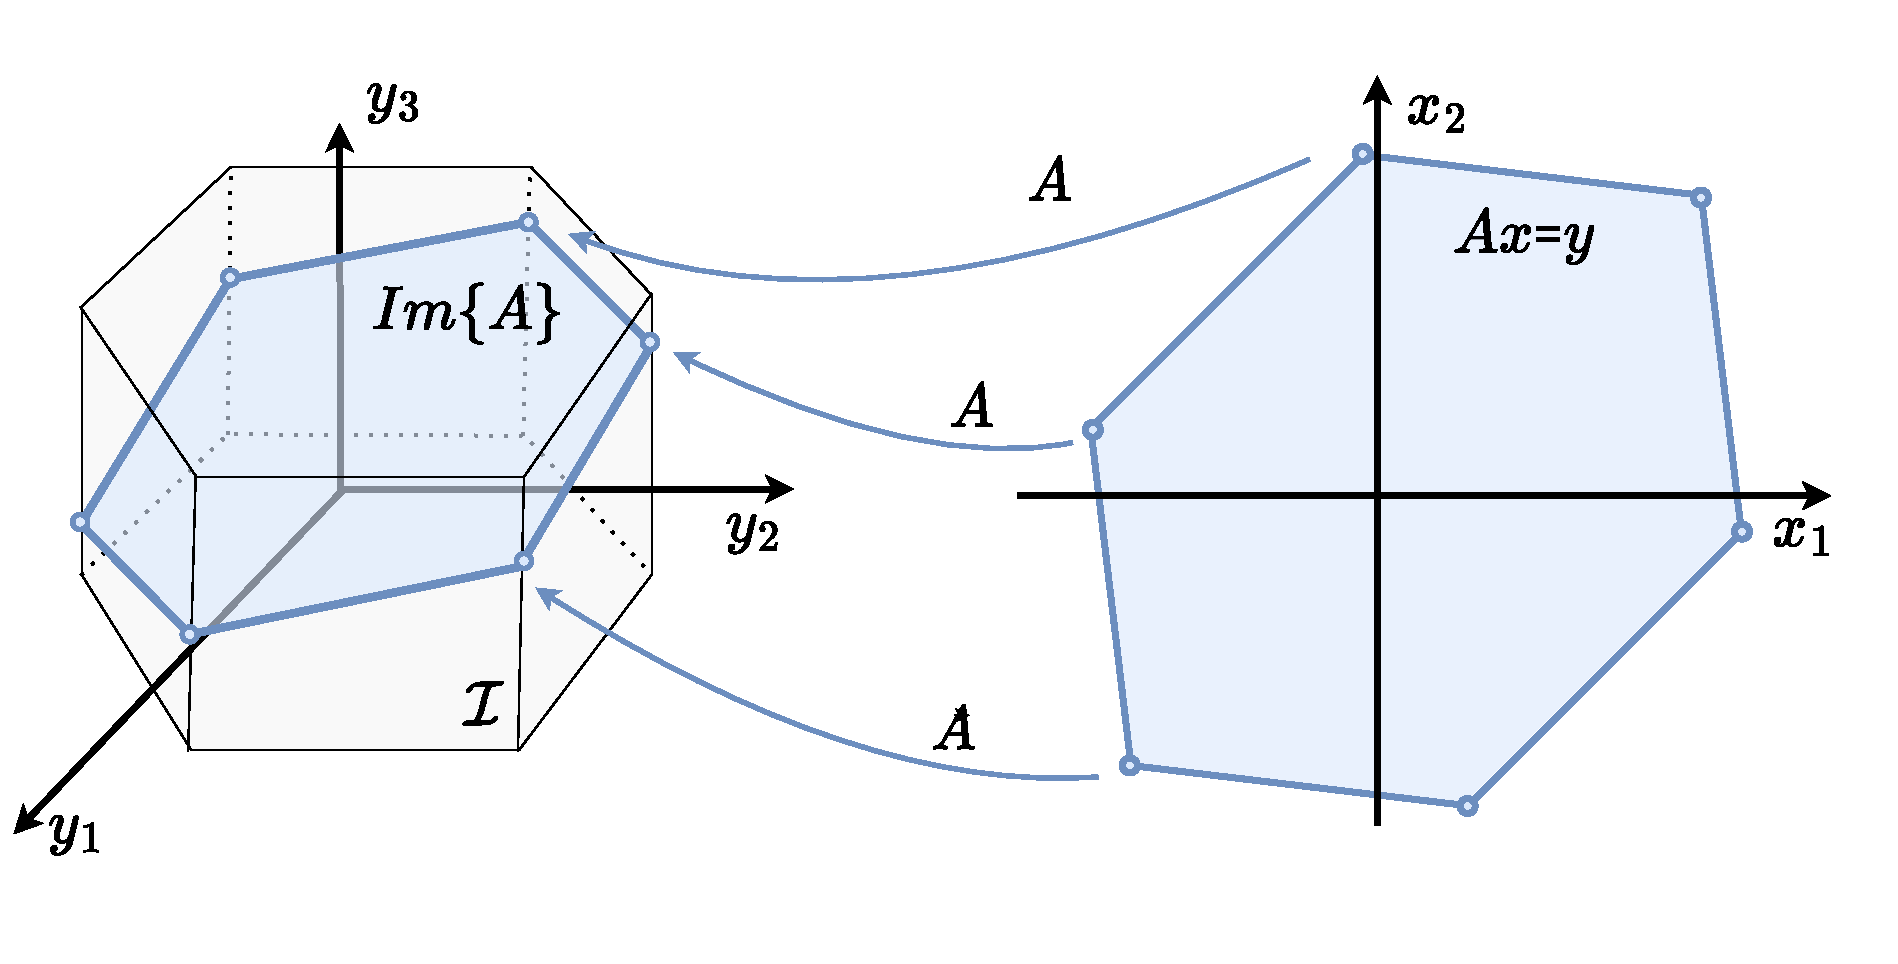
\includegraphics[width=0.8\linewidth]{Chapters/imgs/inter_poly.pdf}
    \caption{An example of constructing an intersection formulation polytope with an $m=2$ dimensional output space and an $n=3$ dimensional input space. The input set $\mathcal{P}_y$ has a polytope form, and its intersection with the image of the matrix $A$ is shown in blue (left). The final polytope $\mathcal{P}_x$ is shown in blue as well (right).}
    \label{fig:inter_poly}
\end{figure}

The geometrical representation of the polytope $\mathcal{P}_x$ defined by (\ref{eq:inter_poly_revist}) is shown on \Cref{fig:inter_poly}, for the example of $n=3$ dimensional input set $\mathcal{P}_y$ and $m=2$ dimensional polytope $\mathcal{P}_x$. 
The resulting polytope $\mathcal{P}_x$ is an affine projection of the intersection of the input polytope $\mathcal{P}_y$ and the image $\img{A}$ of the matrix $A$ into the lower dimensional output space. As shown on \Cref{fig:inter_poly}, the vertices and faces of the polytope $\mathcal{P}_x$ do not correspond to the projection of the vertices and faces of the input polytope $\mathcal{P}_y$. 
Rather, as discussed in \Cref{par:equivalent_proj}, the polytope $\mathcal{P}_x$ is generated by projecting the intersection $\img{A}\cap\mathcal{P}_y$, of the polytope $\mathcal{P}_y$ and the image $\img{A}$ of the matrix $A$, to the output space. 
Therefore, there is a unique mapping between the vertices and faces of the intersection $\img{A}\cap\mathcal{P}_y$, and the vertices and the faces of the polytope $\mathcal{P}_x$, given through the pseudo-inverse inverse \cite{wang2018generalized} of the matrix $A$. 

Algorithms for finding the $\repr{V}$ and $\repr{H}$-representation vary in complexity, depending on the structure of the input set $\mathcal{P}_y$.

\subsubsection{Finding the $\repr{H}$-representation} 
\label{ch:inter_h_rep}
If the input set $\mathcal{P}_y$ is expressed in its $\repr{H}$-representation
\begin{equation}
    \mathcal{P}_y = \{ \bm{y}\in \mathbb{R}^n ~|~H_y\bm{y} \leq \bm{d}_y\}
    \label{eq:step1_inter_h}
\end{equation}
then finding the $\repr{H}$-representation of the polytope $\mathcal{P}_x$ is straightforward, by replacing the vector $\bm{y}$ with $A\bm{x} - \bm{b}_y$ in the equation above
\begin{equation}
    \mathcal{P}_x=\{\bm{x}\in  \mathbb{R}^m~|~ H_yA\bm{x} \leq \bm{d}_y -H_y\bm{b}_y \}
    \label{eq:inter_poly_h_rep}
\end{equation}
Even though this $\repr{H}$-representation (\ref{eq:inter_poly_h_rep}) of the polytope $\mathcal{P}_x$ follows directly from its definition and can be easily expressed, it might not be minimal. This means that even though the equation (\ref{eq:inter_poly_h_rep}) is correct and fully describes the polytope $\mathcal{P}_x$, there might be some redundant half-planes. Many algorithms have been developed over the years for removing the redundant half-planes equations \cite{Paulraj2006}, and their computational complexity is generally equivalent to solving a series of \gls{lp} problems \cite{Telgen1983},\cite[Chapter 7.2]{fukuda2016lecture}. Therefore, depending on the application and the computational complexity of the polytope description necessary, such techniques can be used to reduce the equation (\ref{eq:inter_poly_h_rep}) to the minimal set of linear constraints.

However, if the polytope $\mathcal{P}_y$ is not expressed in $\repr{H}$-representation, in most cases the most efficient strategy is to first transform it to its $\repr{H}$-representation and the apply the manipulation described above. For example if the polytope $\mathcal{P}_y$ is expressed by its $\repr{V}$-representation, 
\begin{equation}
    \mathcal{P}_y = \conv{ \bm{y}_{v1}, ~ \bm{y}_{v2},~ \ldots}
\end{equation}
where $\bm{y}_{vi} \in \mathbb{R}^n$ are the vertices of $\mathcal{P}_y$.  These vertices can be transformed to the $\repr{H}$-representation using the techniques described in \Cref{ch:standard_represtantion_conversion}, which can then be used with the above described approach (\ref{eq:inter_poly_h_rep}) to obtain the $\repr{H}$-representation of the polytope $\mathcal{P}_x$.

Therefore, when it comes to finding the $\repr{H}$-representation of the polytope $\mathcal{P}_x$, the main complexity comes form determining the $\repr{H}$-representation of the input set $\mathcal{P}_y$. The input set $\mathcal{P}_y$, in general case, can have any formulation, not necessarily corresponding neither to the $\repr{V}$ nor to the $\repr{H}$-representation.

Therefore, in the remainder of this section three special cases of the input set formulations are discussed: intersection and projection formulation of the input set $\mathcal{P}_y$, as well as the interval form $\mathcal{I}_y$.

\subsubsection*{Special case: intersection formulation} 
\label{ch:inter_h_special_inter}
If the input set $\mathcal{P}_y$ has the intersection formulation itself
\begin{equation}
    \mathcal{P}_y=\{\bm{y}\in  \mathbb{R}^n~|~ C\bm{y}=\bm{z} + \bm{b}_z, ~ \bm{z} \in \mathcal{P}_z \}
\end{equation}
where $\bm{z}\in\mathcal{R}^k$ is a new its $k$ dimensional input vector, bounded within the set $\mathcal{P}_z$, $\bm{b}_z\in\mathbb{R}^k$ is the bias vector and the matrix $C\in \mathbb{R}^{k\times n}$ is a projector form the $n$ dimensional space to the $k$ dimensional space, where $k\geq n$.

Then the two intersection formulations can be combined into the new polytope $\mathcal{P}_x$, by replacing $\bm{y}$ with $A\bm{x}- \bm{b}_y$
\begin{equation}
    \mathcal{P}_x=\{\bm{x}\in  \mathbb{R}^m~|~ \underbrace{CA}_{A'}\bm{x}=\bm{z} + \underbrace{\bm{b}_z + C\bm{b}_y}_{\bm{b}_z'}, ~ \bm{z} \in \mathcal{P}_z \}
\end{equation}
This new combined polytope has the intersection formulation as well, where the polytope $\mathcal{P}_z$ becomes its input set. Therefore, all the approaches described \Cref{ch:inter_h_rep} are valid for this polytope respectively.

\subsubsection*{Special case: projection formulation} 
The case where the input set $\mathcal{P}_y$ has the projection formulation corresponds to the combined special case called intersection-projection formulation, described in \Cref{ch:inter_proj_form}. 

The most straightforward approach to finding the $\repr{H}$-representation of the polytope $\mathcal{P}_x$ consists in first finding the $\repr{H}$-representation of the input set $\mathcal{P}_y$. Then the above described method  (\ref{eq:step1_inter_h}-\ref{eq:inter_poly_h_rep}) can be used to find the final $\repr{H}$-representation of the polytope $\mathcal{P}_x$.

The common strategies for finding the $\repr{H}$-representation of polytopes with the projection formulation are described in \Cref{ch:projection_algos}.

\subsubsection*{Special case: Interval form $\mathcal{I}_y$}  
\label{par:intersection_interval_algos_h}
\begin{figure}
    \centering
    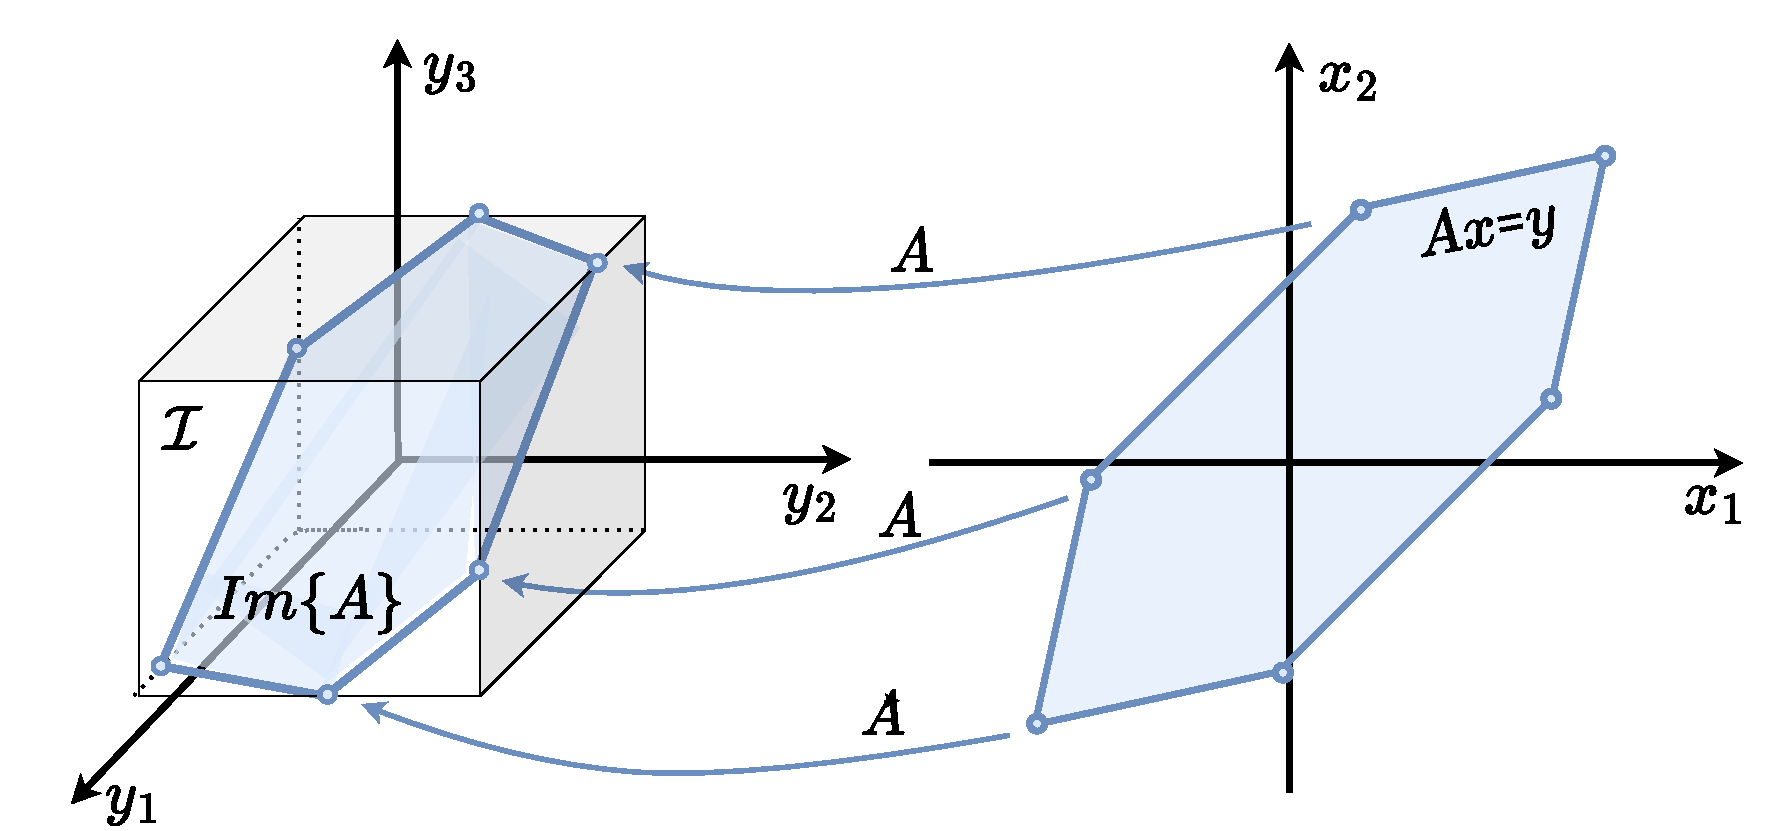
\includegraphics[width=0.8\linewidth]{Chapters/imgs/intersection.pdf}
    \caption{An example of the constructing an intersection formulation polytope with $m=2$ dimensional output space and $n=3$ dimensional input space. The intersection $\img{A} \cap \mathcal{I}_y$ of the hyperrectangle shaped input space $\mathcal{I}_y$ with the image of the matrix $A$ is shown in blue (left). This intersection can be projected to the output space using the inverse of the matrix $A$ to obtain the polytope $\mathcal{P}_x$ (blue right).}
    \label{fig:inter}
\end{figure}

The intersection polytope formulation (\ref{eq:inter_poly_revist}) with the interval limits 
\begin{equation}
    \mathcal{I}_y = \{ \bm{y}\in\mathbb{R}^n ~|~ \bm{y}\in[\bm{y}_{min},\bm{y}_{max}]\}
\end{equation}
is a spacial case of the intersection polytope formulation where the input space limits are defined as independent min-max ranges 
\begin{equation}
    \mathcal{P}_x=\{\bm{x}\in\mathbb{R}^m~ |~ A\bm{x} = \bm{y} + \bm{b}_y,~\bm{y}_{min} \leq  \bm{y} \leq \bm{y}_{max}  \}
    \label{eq:inter_hyp}
\end{equation}
\Cref{fig:inter} graphically represents the construction the polytope $\mathcal{P}_x$ from the input set $\mathcal{I}_y$.

When the input set has the interval form $\mathcal{I}_y$ the $\repr{H}$-representation of the polytope $\mathcal{P}_x$ can be found directly by substituting $\bm{y}$ with $A\bm{x}-\bm{b}_y$ in the interval equation $\bm{y}\in[\bm{y}_{min},\bm{y}_{max}]$ and rewriting it in the matrix from
\begin{equation}
   \underbrace{\begin{bmatrix}
        A\\
        -A
    \end{bmatrix}}_{H_x}\bm{x} \leq \underbrace{\begin{bmatrix}
         \bm{y}_{max} + \bm{b}_y\\
        -\bm{y}_{min} + \bm{b}_y 
    \end{bmatrix} }_{\bm{d}_x}
\end{equation}
where matrix $H_x\in\mathbb{R}^{2n \times m}$ and the vector $\bm{d}_x\in\mathbb{R}^{2n}$ can be used to express the $\repr{H}$-representation of the polytope $\mathcal{P}_x$
\begin{equation}
    \mathcal{P}_x=\{\bm{x}\in\mathbb{R}^m |~ H_x\bm{x} \leq \bm{d}_x \}
    \label{eq:inter_h_rep}
\end{equation}
However, as discussed at the beginning of \Cref{ch:inter_h_rep}, additional steps might be necessary to remove the redundant half-plane equations within the matrix $H_x$ and the vector $\bm{d}_x$.


\subsubsection{Finding the $\repr{V}$-representation} 
\label{ch:inter_v_rep}
Finding the $\repr{V}$-representation of polytopes with the intersection formulation, is a much more complex operation with respect to finding the $\repr{H}$-representation. 

In general, finding the $\repr{V}$-representation of the polytope $\mathcal{P}_x$, is performed by first finding its $\repr{H}$-representation, as described in the previous section (\Cref{ch:inter_h_rep}). Then, depending on the size of the problem, different standard representation conversion algorithms, described in \Cref{ch:standard_represtantion_conversion}, can be used to obtain its $\repr{V}$-representation.

However, as the special case of the intersection formulation, where the input set has interval shape $\mathcal{I}_y$, is particularly present in the robotics literature, several efficient algorithms have been proposed for finding its $\repr{V}$-representation directly.



\subsubsection*{Special case: Interval form $\mathcal{I}_y$}
\label{par:intersection_interval_algos_v}

When the input set has interval shape $\mathcal{I}_y$, the compact form of this polytope  $\mathcal{P}_x$ with the intersection formulation can be expressed as
\begin{equation}
    \mathcal{P}_x=\{\bm{x}\in\mathbb{R}^m ~ |~ A\bm{x} = \bm{y} + \bm{b}_y,~ \bm{y} \in [\bm{y}_{min},~  \bm{y}_{max}]  \}
    \label{eq:inter_hyp_revisit}
\end{equation}

Several efficient algorithms were developed for finding all the vertices of polytopes with this formulation. These algorithms, exploit the geometry of the problem and provide better efficiency than the standard conversion INA or GTA based methods.

An efficient algorithm for vertex enumeration of the intersection type polytope is proposed by \citet{gouttefarde_versatile_2015}. The algorithm assumes that the output space dimension is always $m=2$, in which case, the polytope $\mathcal{P}_x$ becomes a 2D polygon. The algorithm then exploits the 2D geometry of the problem and efficiently navigates the boundaries of the polygon in search for extremities. However, this algorithm does not scale well to higher dimensional problems.

A different algorithm, finding the $\repr{V}$-representation of the intersection polytope $\mathcal{P}_x$ with interval limits $\mathcal{I}_y$, is proposed by \citet{chiacchio_evaluation_1996}. The algorithm leverages the hyperrectangle geometry of the interval input set $\mathcal{I}_y$ and performs an efficient exhaustive search through its faces. This algorithm has been improved by \citet{sasaki2011vertex}, significantly reducing the computational complexity by exploiting the geometry of the intersection of the hyperrectangle (interval) $\mathcal{I}_y$ and the image of matrix $\img{A}$. Moreover, this improved algorithm is based on the equivalent projection formulation of the intersection polytope, described in the \Cref{par:equivalent_proj}.
\begin{equation}
\mathcal{P}_x=\{\bm{x}\in\mathbb{R}^m ~|~ \bm{x} = A^+\bm{y} + A^+\bm{b}_y,~ \bm{y} \in \img{A}\cap[\bm{y}_{min},\bm{y}_{max}]\}
\label{eq:inter_hyp_inter}
\end{equation}

Both of these algorithms, \citet{chiacchio_evaluation_1996} and \citet{sasaki2011vertex}, are based on the efficient exhaustive search of the hyperrectangle $\mathcal{I}_y$ faces. However, the number of faces of the hyperrectangle grows exponentially with the input space dimension
$$
N_{n,k}= 2^{n-k}\binom{n}{k}
$$
where $n$ is the dimension of the input space, $N_{n,k}$ is the number of the $k$ dimensional hyperrectangle faces. Therefore,  as the dimension of the input space $n$ grows, the computational efficiency of these algorithms decreases exponentially.

\subsection{Strategies for the projection formulation}
\label{ch:projection_algos}

This section brings a short overview of methods used for the transformation of polytopes with projection formulation, described in \Cref{ch:proj_formulaiton}, into their respective $\repr{V}$ and $\repr{H}$-representation.

\label{ch:proj_poly_chapter}
\begin{figure}
    \centering
    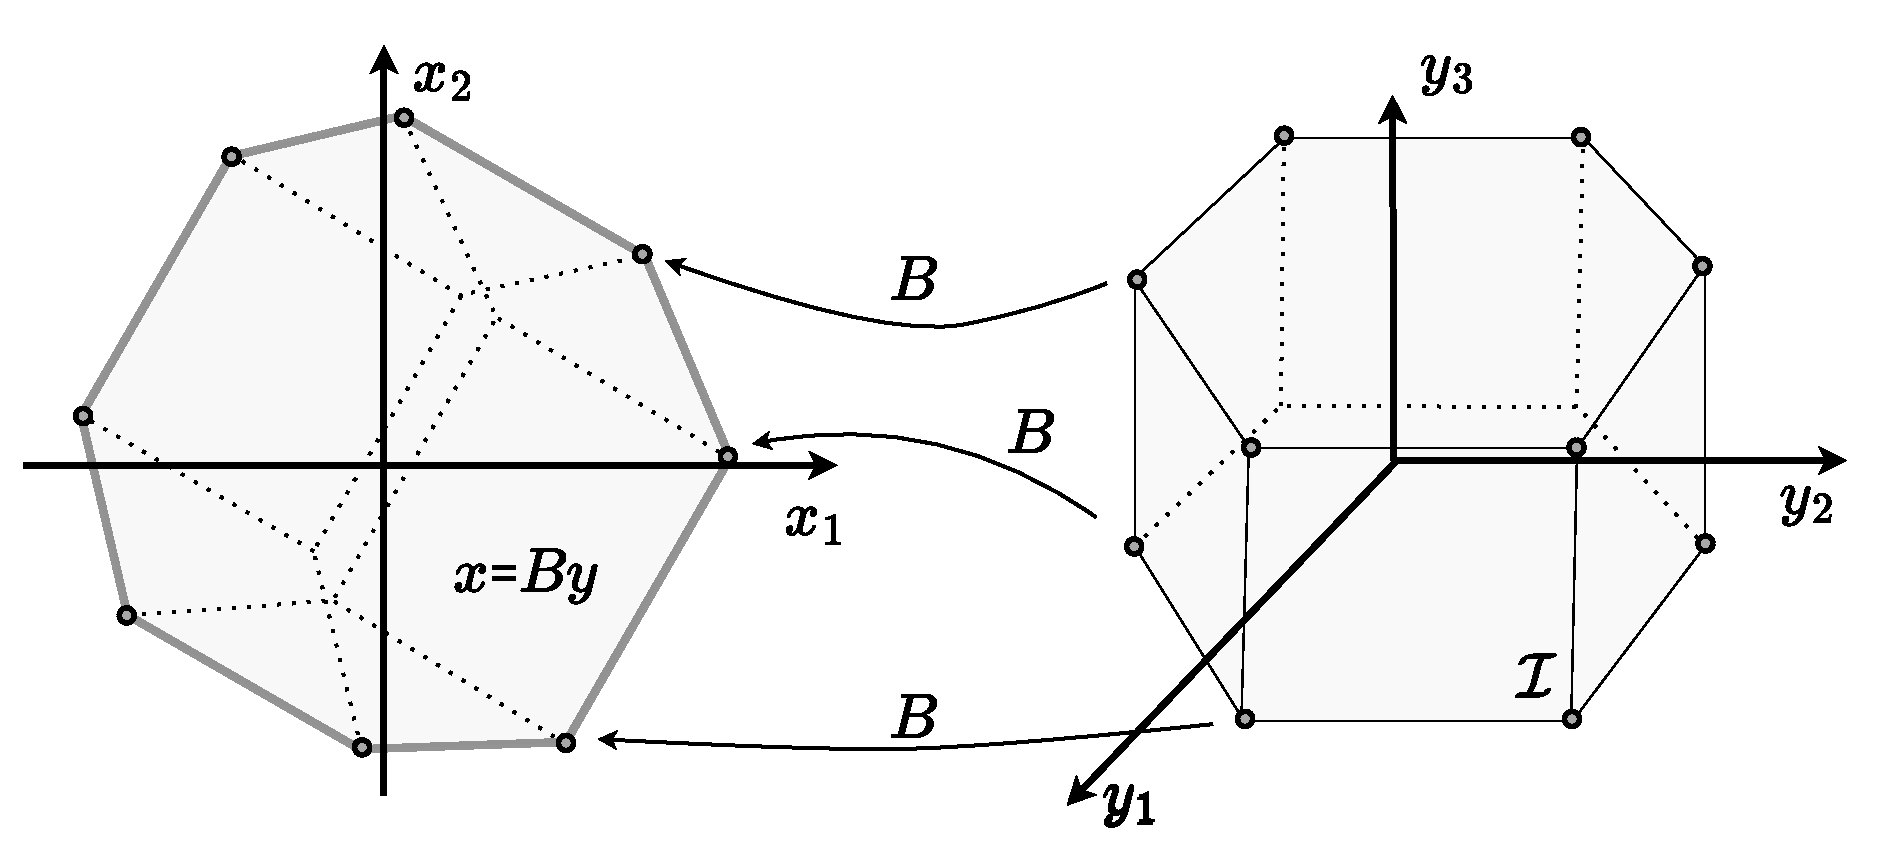
\includegraphics[width=0.7\linewidth]{Chapters/imgs/proj_poly.pdf}
    \caption{An example of the constructing a projection formulation polytope with $m=2$ dimensional output space and $n=3$ dimensional input space, where the input space $\mathcal{P}_y$ has a polytope shape. In this formulation, the whole input space $\mathcal{P}_y$ (grey) is projected using the matrix $B$ to the output space to obtain the polytope $\mathcal{P}_x$ (blue). }
    \label{fig:proj_poly}
\end{figure}

The projection polytope (\ref{eq:proj_poly}) with polytope input set $\mathcal{P}_y$ can be expressed as
\begin{equation}
    \mathcal{P}_x=\{\bm{x}\in\mathbb{R}^m |~ \bm{x} = B\bm{y} + \bm{b}_x,~\bm{y} \in \mathcal{P}_y  \}
    \label{eq:proj_poly_1}
\end{equation}
where $\bm{y}\in\mathbb{R}^n$ is an $n$ dimensional input vector, $\bm{x},\bm{b}_x\in\mathbb{R}^m$ are the $m$ dimensional output vector and bias, while $B\in\mathbb{R}^{m\times n}$ is a transformation matrix from input to the output space.

The geometrical representation of the polytope $\mathcal{P}_x$ defined by (\ref{eq:proj_poly_1}) is shown on \Cref{fig:proj_poly}, for the example of $n=3$ dimensional polytope $\mathcal{P}_y$ and $m=2$ dimensional polytope $\mathcal{P}_x$. The resulting polytope $\mathcal{P}_x$ is an affine projection of the input polytope $\mathcal{P}_y$ into the lower dimensional output space. Furthermore, the vertices and the faces of the polytope $\mathcal{P}_x$ correspond to the subset of the projected vertices and faces of the input polytope $\mathcal{P}_y$. 

Given the structure of the input set $\mathcal{P}_y$ algorithms for finding the $\repr{V}$ and $\repr{H}$-representation vary in complexity. 

\subsubsection{Finding the $\repr{V}$-representation}
\label{ch:proj_algos_v}
If the input set polytope $\mathcal{P}_y$ is expressed using its vertex or $\repr{V}$-representation
\begin{equation}
    \mathcal{P}_y = \conv{ \bm{y}_{v1}, ~ \bm{y}_{v2},~ \ldots}
    \label{eq:proj_v_step1}
\end{equation}
where $\bm{y}_{vi}\in\mathbb{R}^n$ are the vertices of the polytope $\mathcal{P}_y$, the vertices of the projection formulation polytope (\ref{eq:proj_poly_1}) can then be found by projecting the vertices of $\mathcal{P}_y$ to the output space using the matrix $B \in \mathbb{R}^{m\times n}$ and calculating their Convex-Hull $\conv{\cdot}$
\begin{equation}
    \mathcal{P}_x= \conv{ B\bm{y}_{v1}, ~ B\bm{y}_{v2},~ \ldots}
    \label{eq:proj_v_step2}
\end{equation}
The Convex-Hull algorithm finds the $\repr{V}$-representation of the projection polytope directly, as the vertices of the polytope $\mathcal{P}_x$ are a subset of the projected vertices $\bm{y}_{vi}$ of the input polytope $\mathcal{P}_y$, as shown in the example on \Cref{fig:proj_poly}. 

If the input polytope $\mathcal{P}_y$ is expressed using its half-plane or $\repr{H}$-representation, 
\begin{equation}
    \mathcal{P}_y = \{ \bm{y}\in\mathbb{R}^n ~|~H_y\bm{y} \leq \bm{d}_y\}
\end{equation}
there are two main approaches decoupling the problem.

The first and straight-forward approach consists in finding the $\repr{V}$-representation of the input set $\mathcal{P}_y$ first, using the standard representation conversion methods described in \Cref{ch:standard_represtantion_conversion}. Then the above described procedure (\ref{eq:proj_v_step1}-\ref{eq:proj_v_step2}) can be used to find the $\repr{V}$-representation of  $\mathcal{P}_x$. However, in many cases, when the input space dimension $n$ is high or if the geometry of the polytope  $\mathcal{P}_y$ is complex (large number of faces and vertices), finding its $\repr{V}$-representation might be computationally demanding. 

The second approach, more efficient in many cases, consists in finding the $\repr{H}$-representation of the polytope $\mathcal{P}_x$ directly from the input set's $\repr{H}$-representation. One of the most well known algorithms for projecting the $\repr{H}$-representation of polytopes is arguably the \gls{fme} described by \citet{dantzig1973fourier}.  This algorithm uses an iterative inequality elimination method to isolate the set of half-plane equations bounding the final polytope $\mathcal{P}_x$. However, this approach has an exponential complexity with the dimension of the input space $n$ \cite{Talaashrafi2020complexity}, and additionally it does not guarantee a minimal representation \cite{Monniaux2010}. A more efficient algorithm is introduced by \citet{jones2004equality} called \gls{esp}. As opposed to \gls{fme}, this algorithm is \textit{output sensitive}, having its execution time proportional to the complexity of the final polytope $\mathcal{P}_x$ (it number of faces and vertices), making it particularly well suited to the high dimensional input spaces $\mathbb{R}^n$. A more in depth comparison of these methods, as well their comparison to several other polytope projection algorithms, is brought in the work by \citet{Gl_le_2018}. Once the $\repr{H}$-representation of the polytope $\mathcal{P}_x$ is obtained using one of these methods, the standard representation conversion methods can be used to obtain the $\repr{V}$-representation of the polytope $\mathcal{P}_x$ defined in the $m$ dimensional output space.

The same two approaches can be used in the general case, where the input set $\mathcal{P}_y$ does not correspond neither to the $\repr{V}$ nor to the $\repr{H}$-representation. The choice of the more suitable one depends on the efficiency of transforming the input set $\mathcal{P}_y$ into its $\repr{V}$ or $\repr{H}$-representation. 

In remaining part of this section three special cases of the input set formulation are discussed: intersection and projection formulation of the input set $\mathcal{P}_y$, as well as the interval form $\mathcal{I}_y$.

\subsubsection*{Special case: intersection formulation} If the input set $\mathcal{P}_y$ has the intersection formulation, then the formulation of the polytope $\mathcal{P}_x$ corresponds to the projection-intersection formulation, the combined special case  described in \Cref{ch:proj_inter_form}.

The $\repr{H}$ and $\repr{V}$-representations of the input set $\mathcal{P}_y$, with intersection formulation, can be obtained using the strategies discussed in \Cref{ch:intersection_algos}. As discussed in \Cref{ch:intersection_algos}, in general, the $\repr{H}$-representation of intersection polytopes can be found more efficiently than the $\repr{V}$-representation, making the second approach described in \Cref{ch:proj_algos_v} better suited.


\subsubsection*{Special case: projection formulation} 
If the input set $\mathcal{P}_y$ has the projection formulation itself
\begin{equation}
    \mathcal{P}_y=\{\bm{y}\in  \mathbb{R}^n~|~ \bm{y}=D\bm{z} + \bm{b}_y, ~ \bm{z} \in \mathcal{P}_z \}
\end{equation}
where $\bm{z}\in\mathcal{R}^k$ is its $k$ dimensional input vector, bounded within the set $\mathcal{P}_z$, $\bm{b}_y\in\mathbb{R}^n$ is the bias vector, and the matrix $D\in \mathbb{R}^{n\times k}$ is a projection matrix form the $k$ dimensional space to the $n$ dimensional space.

Then the two projection formulations can be combined into the new polytope $\mathcal{P}_x$, by replacing the $\bm{y}$ with $D\bm{z} + \bm{b}_y$ in initial formulation of $\mathcal{P}_x$ (\ref{eq:proj_poly_1}).
\begin{equation}
    \mathcal{P}_x=\{\bm{x}\in  \mathbb{R}^m~|~ \bm{x}=\underbrace{BD}_{B'}\bm{z} + \underbrace{B\bm{b}_z + \bm{b}_x}_{\bm{b}_x'}, ~ \bm{z} \in \mathcal{P}_z \}
\end{equation}
This new formulation corresponds to the projection formulation as well. Therefore, the same approaches described in \Cref{ch:proj_algos_v} can be used to find its $\repr{V}$-representation respectively.

\subsubsection*{Special case: Interval form $\mathcal{I}_y$} 


\begin{figure}
    \centering
    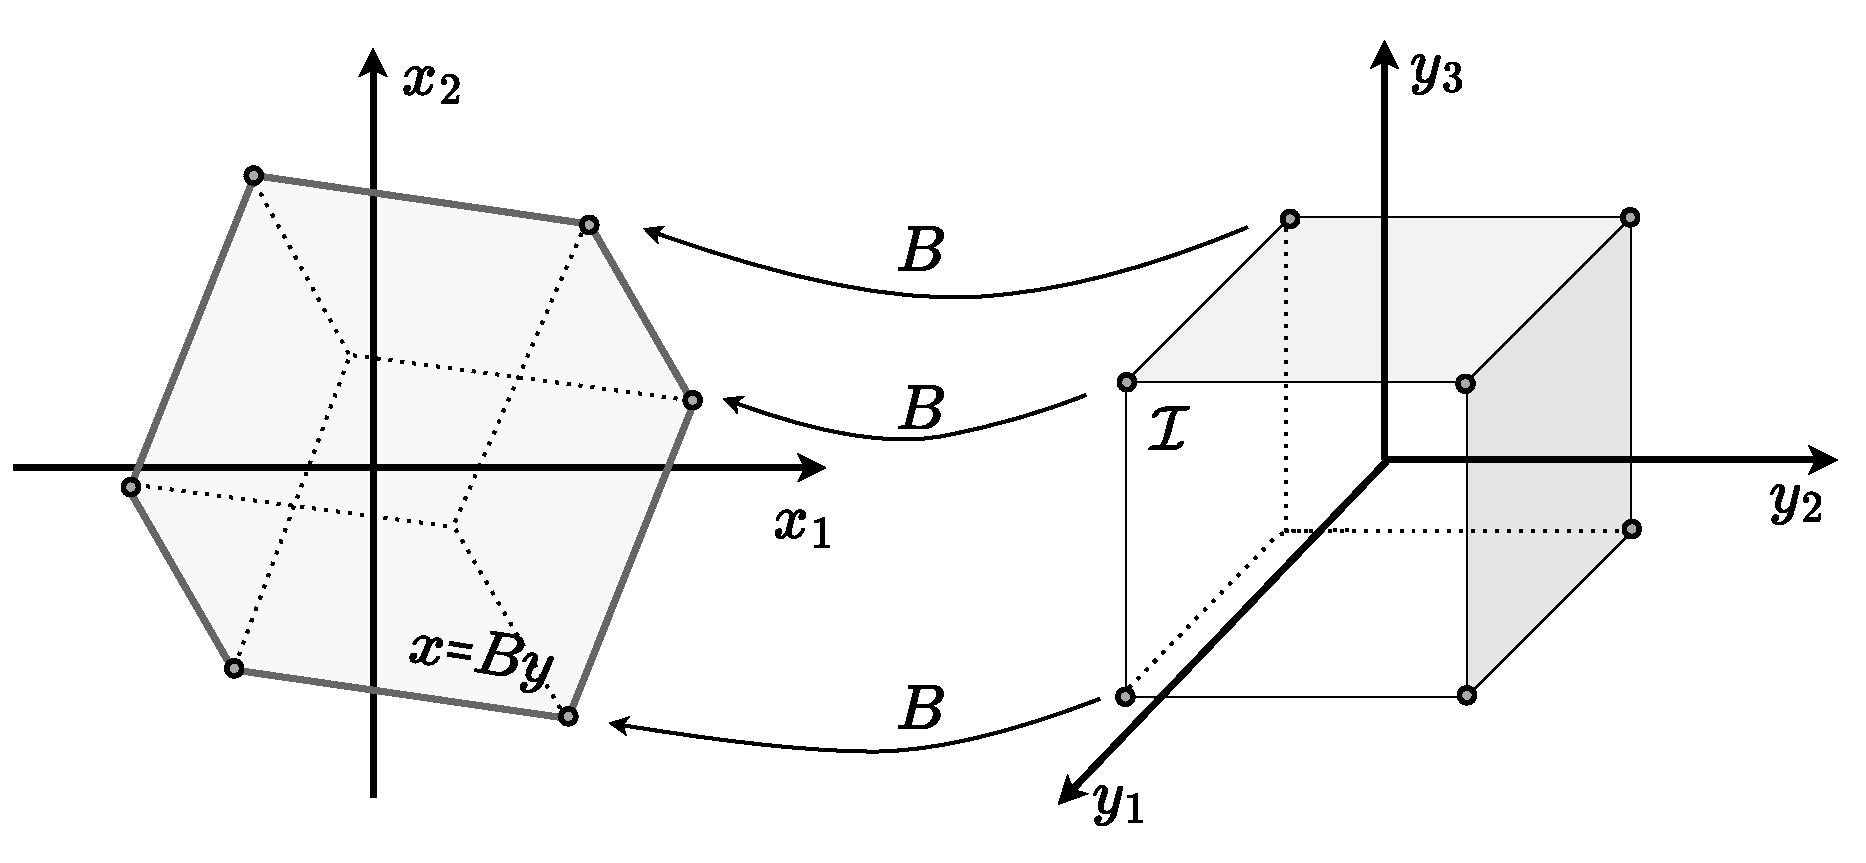
\includegraphics[width=0.8\linewidth]{Chapters/imgs/projection.pdf}
    \caption{An example of the constructing a projection formulation polytope with $m=2$ dimensional output space and $n=3$ dimensional input space, where the input space $\mathcal{I}_y$ has a hyperrectangle (interval) shape. In the projection formulation, the whole input space $\mathcal{I}_y$ (grey) is projected using the matrix $B$ to the output space to obtain the polytope $\mathcal{P}_x$ (blue). }
    \label{fig:proj}
\end{figure}

The projection polytope formulation $\mathcal{P}_x$ with the interval limits $\mathcal{I}_y$
\begin{equation}
    \mathcal{I}_y = \{ \bm{y}\in\mathbb{R}^n ~|~ \bm{y}\in[\bm{y}_{min},\bm{y}_{max}]\}
\end{equation}
is a spacial case of the projection polytope formulation which can be compactly expressed as
\begin{equation}
    \mathcal{P}_x=\{\bm{x}\in\mathbb{R}^m |~ \bm{x} = B\bm{y} + \bm{b}_x,~\bm{y}_{min} \leq  \bm{y} \leq \bm{y}_{max}  \}
    \label{eq:proj_hyp}
\end{equation}
\Cref{fig:proj} graphically represents the construction the polytope $\mathcal{P}_x$ from the input set $\mathcal{I}_y$.

The most straight-forward way of finding the vertices $\bm{x}_{vi}\in\mathbb{R}^m$ of the projection polytope $\mathcal{P}_x$ is by first enumerating the $2^n$ vertices $\bm{y}_{vi}\in\mathbb{R}^n$ of the hyperrectangle  (interval) $\mathcal{I}_y$, by creating a list of all the combinations of the minimal $\bm{y}_{min}$ and maximal $\bm{y}_{max}$ values of $\bm{y}$
\begin{equation}
    \bm{y}_{v1} = \begin{bmatrix}
        y_{1,min}\\
        y_{2,min}\\
        \ldots\\
        y_{n,min}\\
    \end{bmatrix},\quad
    \bm{y}_{v2} = \begin{bmatrix}
        y_{1,max}\\
        y_{2,min}\\
        \ldots\\
        y_{n,min}\\
    \end{bmatrix},\qquad\ldots,\qquad
    \bm{y}_{v2^n} = \begin{bmatrix}
        y_{1,max}\\
        y_{2,max}\\
        \ldots\\
        y_{n,max}\\
    \end{bmatrix} 
\end{equation}
Then these vertices can be projected to the lower dimensional output space $\mathbb{R}^m$ using the projection matrix $B\in \mathbb{R}^{m\times n}$, where the polytope $\mathcal{P}_x$ can be found by calculating the Convex-Hull $\conv{\cdot}$ of the projected points.
\begin{equation}
    \mathcal{P}_x = \conv{B\bm{y}_{v1},B\bm{y}_{v2},~\ldots, ~ B\bm{y}_{v2^n}}
\end{equation}

The complexity of this approach depends on two factors. The dimension of the of the input space $n$ and the dimension of the output space $m$. The number of vertices of the hyperrectangle (interval) grows exponentially ($2^n$) with the dimension of the input space $n$, and constructing a matrix of $2^n \times n$ entries can become impractical. On the other hand, as this approach requires a Convex-Hull algorithms, which are executed in the $m$-dimensional output space, the dimension $m$ might make the Convex-Hull algorithm impractical as their complexity grows significantly with the dimension of the space $m$ \cite{Barber1996}.

Therefore for higher dimensional output spaces (typically $m\geq 4$) and input spaces (causing the memory issues due to  $2^n \times n$ matrix construction) a more efficient approach might be to first calculate the $\repr{H}$-representation of this polytope, using the methods described in the following section, and then use standard representation conversion methods (\Cref{ch:standard_represtantion_conversion}), to find its $\repr{V}$-representation.


\subsubsection{Finding the $\repr{H}$-representation}
\label{ch:proj_algos_h}

If the input polytope $\mathcal{P}_y$ is expressed using its half-plane or $\repr{H}$-representation, 
\begin{equation}
    \mathcal{P}_y = \{ \bm{y}\in\mathbb{R}^n ~|~H_y\bm{y} \leq \bm{d}_y\}
\end{equation}
the straight-forward approach consists in decoupling the problem and find the $\repr{V}$-representation first, using the standard representation conversion methods  described in \Cref{ch:standard_represtantion_conversion}, then follow the above described procedure (\Cref{ch:proj_algos_v}) to find the $\repr{V}$-representation of $\mathcal{P}_x$. 

As described in the previous section, in many cases, when the input space dimension $n$ is high or if the geometry of the polytope  $\mathcal{P}_y$ is complex (large number of faces and vertices), finding its $\repr{V}$-representation might be computationally demanding. In those cases, if the $\repr{H}$-representation of the polytope $\mathcal{P}_y$ is available, the $\repr{H}$-representation of the polytope $\mathcal{P}_x$ can be found directly using the algorithms such as \gls{fme} and \gls{esp}. 

These same two approaches can be used in the general case, where the input set $\mathcal{P}_y$ does not correspond neither to the $\repr{V}$ nor to the $\repr{H}$-representation. The choice of the more suitable one depends on the efficiency of transforming the input set $\mathcal{P}_y$ into its $\repr{V}$ or $\repr{H}$-representation. 

\subsubsection*{Special case: Interval form $\mathcal{I}_y$} 

The projection polytope formulation $\mathcal{P}_x$ with the interval limits $\mathcal{I}_y$ can be compactly expressed
\begin{equation}
    \mathcal{P}_x=\{\bm{x}\in\mathbb{R}^m |~ \bm{x} = B\bm{y} + \bm{b}_x,~\bm{y}_{min} \leq  \bm{y} \leq \bm{y}_{max}  \}
    \label{eq:proj_hyp_1}
\end{equation}

Apart from the two approaches described at the beginning of this section (\Cref{ch:proj_algos_h}), there are several more efficient algorithms introduced in the literature, specific for this formulation and typically exploiting the polytope's zonotope structure.

One such  efficient algorithm, exploiting the geometry of the formulation (\ref{eq:proj_hyp_1}) of the projection polytope $\mathcal{P}_x$ with interval limits $\mathcal{I}_y$, is introduced by \citet{Bouchard2009} and improved by Gouttefarde and Krut \cite{hyper_psm}. It is often referred to as \gls{hpsm}. This algorithm finds the minimal $\repr{H}$-representation of the polytope (\ref{eq:proj_hyp_1}) by efficiently performing the exhaustive search of all the possible half-plane combinations corresponding to the $m-1$ dimensional polytope $\mathcal{P}_x$ faces. Even-though much more efficient than the \glsxtrfull{fme}, this algorithm still has considerable (binomial) complexity, as it relies on the exhaustive search in the $n$ dimensional input space where the number $N_h$ of hyper-planes to be tested equals to 
$$N_h = \binom{n}{m-1}$$

\subsection{Polytope approximation strategies}
\label{ch:approximation_algos}

Exact vertex and facet enumeration methods, such as the standard representation conversion methods described in \Cref{ch:standard_represtantion_conversion} or more specific methods for the projection and the intersection formulation described in \Cref{ch:intersection_algos} and \Cref{ch:projection_algos}, rely on different versions of exhaustive search in the $n$-dimensional input space, which is often higher dimensional than the output space $n> m$. Their execution time is typically exponential, or polynomial in the best case, with respect to the dimension of the input space $n$, the number of vertices and the faces of the input set $\mathcal{P}_y$ and the final polytope $\mathcal{P}_x$ \cite{Dyer1983}. Therefore, in cases where the input space is much higher dimensional than the output space $n\gg m$ or when the polytopes $\mathcal{P}_x$ and $\mathcal{P}_y$ have complex geometries (large number of faces and vertices), such approaches may not be practically viable for interactive, in-the-loop, applications. 

To overcome this issue, various approximate approaches, such as the \gls{rsm} \cite{agarwal1993ray} and the \gls{chm} \cite{lassez1992quantifier} have been developed, reducing the complexity and improving the execution time. 

\begin{wrapfigure}{r}{0.35\linewidth}
% \vspace{-0.5cm}
% \begin{framed}
    \centering
    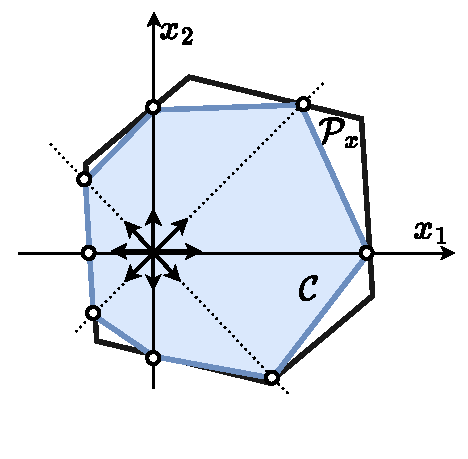
\includegraphics[width=\linewidth]{Papers/images/rsm.pdf}
    \caption{An example of the approximation $\mathcal{C}$ of the 2D ($m\!=\!2$) polytope $\mathcal{P}_x$ using a \gls{rsm} algorithm. The input space is sampled with 8 rays. }
    \label{fig:rsm}
% \end{framed}
\end{wrapfigure}
The \gls{rsm} algorithms are relatively simple to setup as they rely on different forms of sampling (shooting rays) of the polytope $\mathcal{P}_x$, in the low dimensional output space. Their execution time is proportional to the number of sampling directions (rays shot), therefore, by choosing an appropriate sampling strategy, the \gls{rsm} algorithms can provide an efficient approximation of the polytope $\mathcal{P}_x$. However, these algorithms do not provide any bound on their estimation error and rely highly on hand tuned initial parameters. \Cref{fig:rsm} shows a visual example of a \gls{rsm} approximation of a polygon $\mathcal{P}_x$ using uniform sampling in the output space with 8 rays.

The \gls{chm} algorithms, first introduced by \citet{lassez1992quantifier, Huynh2005PracticalIO}, propose an efficient iterative approximation of the polytope $\mathcal{P}_x$, while at the same time avoiding the complexity of the exhaustive search. The CHM algorithms simplify the final polytope $\mathcal{P}_x$ geometry by removing the need to find all the faces and vertices of the polytope. Such algorithms are usually defined in the lower-dimensional output space $\bm{x}\in \mathbb{R}^m$ making them \textit{output sensitive}, having the execution time proportional to the number of vertices and the faces of the output space polytope $\mathcal{P}_x$. In addition to searching in the lower $m$ dimensional output space, they enable finding an efficient inner (or outer) approximation of the polytope $\mathcal{P}_x$, while satisfying a user defined level of accuracy. Finally, they find both the vertices and the faces of the polytope $\mathcal{P}_x$ at the same time, providing both $\repr{V}$ and the $\repr{H}$-representation \cite{Gl_le_2018}.


The execution of a typical \gls{chm} algorithm consists in two phases. In the first phase an initial approximation of the polytope $\mathcal{P}_x$ is constructed finding a subset of $m+1$ vertices forming an initial $m$-dimensional Convex-Hull $\mathcal{C}$ approximation of the polytope $\mathcal{P}_x$. In the second phase, the Convex-Hull approximation $\mathcal{C}$ is refined iteratively until the desired accuracy is reached. The \gls{chm} algorithms use a sequence of \glspl{lp} to find new vertices of the polytope in each iteration, followed by the Convex-Hull algorithm to group them to the faces. An example of the \gls{chm} algorithm iterations for $m=2$ output space is shown on \Cref{fig:chm}.   

The \gls{chm} algorithms have several limitations though. The resolution of the algorithms relies on the iterative application of the Convex-Hull algorithm which complexity grows exponentially for output space dimensions $m > 3$ \cite{Barber1996}. As a result, the applications of these methods have so far been limited to the low-dimensional output spaces $m\leq3$. Additionally, as different polytope formulations require different \gls{lp} formulations, the implementations of these methods are often somewhat specific to their respective applications. 

There are several examples in the literature where the approximation based methods were used for improving the efficiency of different computationally expensive polytope evaluation problems. \citet{Bretl2008} have proposed a \gls{chm} based algorithm for approximating 2D ($m\!=\!2$) polytopes in the context of legged robot locomotion. \citet{DelPrete2016Fast} recently proposed an efficiency improvement of this algorithm, and \citet{Herve2018} extended it to the 3D ($m\!=\!3$) use-cases. This algorithm calculates the inner and outer approximation of the polytope $\mathcal{P}_x$ at the same time, while its accuracy condition can be set a as desired ratio between the inner and outer approximation volumes. \citet{Ponce1995} have introduced a derivative of the \gls{chm} algorithm to calculate the 2D, 3D and 4D ($m\!=\!2,3,4$) polytopes in the context of grasping objects with multiple fingers. While \citet{Xu2008projection} used a \gls{chm} algorithm in the context in the context of information theory. Both of these algorithms find all vertices and faces of the output polytope $\mathcal{P}_x$, without exploiting \gls{chm}'s approximation capacity. Furthermore, \citet{carmichael_estimating_2013,carmichael2011Towards} used an \gls{rsm} algorithm for approximating 2D and 3D ($m\! =\! 2,3$) polytopes in the context of human force capacity estimation, based on a musculoskeletal model. In order to enable real-time execution, their \gls{rsm} implementation relies on the uniform sampling in the output space.

 
\begin{figure}
    \centering
    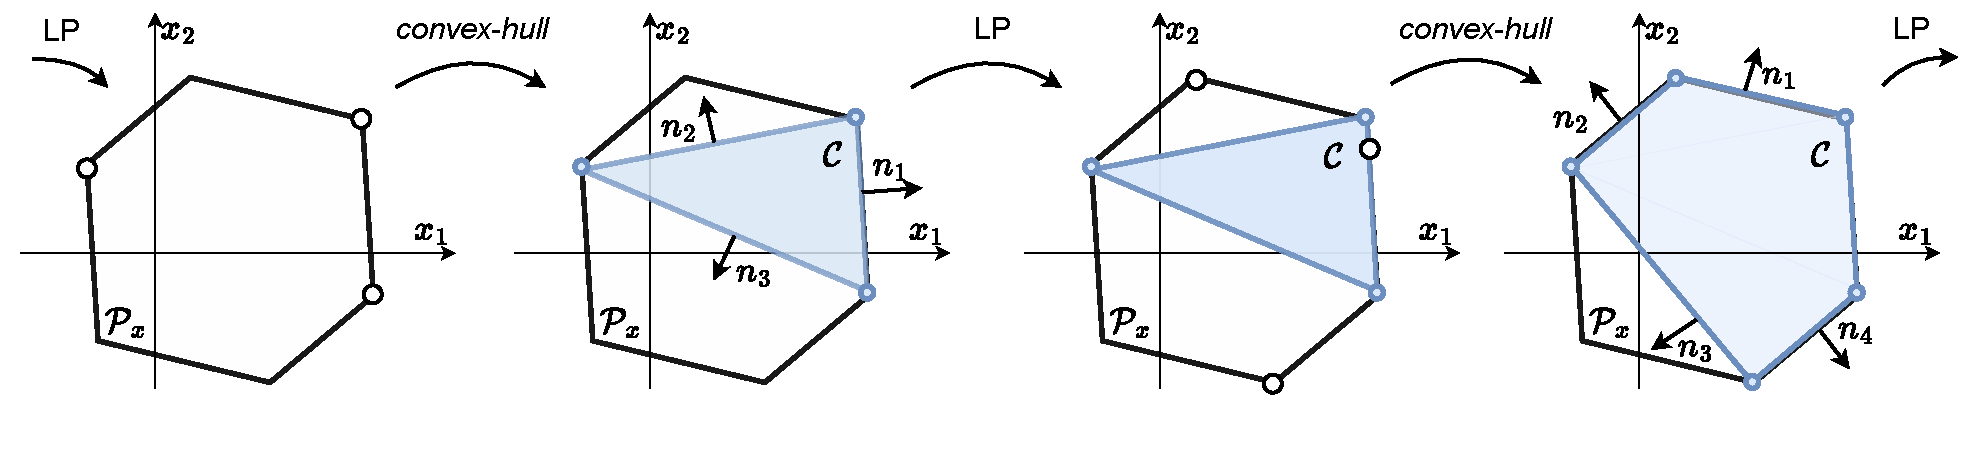
\includegraphics[width=\linewidth]{Papers/images/chm_algo.pdf}
    \caption{This figure shows the procedure of successive approximation of the polytope $\mathcal{P}_x$ using the \gls{chm} algorithm. The face normal vectors $\bm{n}_i$ of the Convex-Hull $\mathcal{C}$ are used with \gls{lp} to find new vertices which are then used to update the Convex-Hull $\mathcal{C}$ and furthermore improve the approximation of the polytope.}
    \label{fig:chm}
\end{figure}

In summary, when the complexity of the polytope $\mathcal{P}_x$ transformation does not permit using standard exact methods in the practical applications, especially when the dimension $n$ of the input space is high while the dimension of the output space $m$ is reasonably low $m\leq3$, polytope approximation methods, such as \gls{rsm} and \gls{chm} algorithms, provide a more efficient solutions. The \gls{rsm} algorithms provide a fast sampling based approximation, however without any guarantees on the approximation error or accuracy. On the other hand, \gls{chm} algorithms use an efficient iterative approach to the polytope approximation, while at the same time being capable of guaranteeing the maximal approximation error.

\subsection{Synthesis of transformation strategies}
\label{ch:overview_algo_synthesis}
\afterpage{
\begin{landscape}
\vspace*{\fill}
\begin{table}[!h]
    \hspace{-2cm}   
    \scalefont{0.85}
    \centering
    \begin{tabular}{|l|c|c|c|c|c|c|c|c|c|c|c|c|c|c|c|c|c|c|}
    \hline
         Formulation & \multicolumn{2}{c|}{ \begin{tabular}{@{}c@{}@{}} Generic (Unified) \\ $A \bm{x}=B\bm{y} + \bm{b}$, $\bm{y}\in \mathcal{P}_y$ \\ \Cref{eq:generic_polyt_view_revisit}\end{tabular}} &\multicolumn{8}{c|}{ \begin{tabular}{@{}c@{}@{}}Projection (Proj.) \\ $ \bm{x}=B\bm{y} + \bm{b}_x$, $\bm{y}\in \mathcal{P}_y$ \\ \Cref{eq:proj_poly}
         \end{tabular}} & \multicolumn{8}{c|}{\begin{tabular}{@{}c@{}@{}}Intersection (Int.)\\ $ A\bm{x}=\bm{y} + \bm{b}_y$, $\bm{y}\in \mathcal{P}_y$ \\ {\Cref{eq:inter_poly}}\end{tabular}} \\
    \hline
         \begin{tabular}{@{}l@{}}Finding \\ representation\end{tabular} &
         \hspace*{0.5cm}$\repr{H}$\hspace*{0.5cm} & $\repr{V}$ & \multicolumn{3}{c|}{$\repr{H}$}& \multicolumn{5}{c|}{$\repr{V}$}& \multicolumn{3}{c|}{$\repr{V}$}& \multicolumn{5}{c|}{$\repr{H}$}\\
    \hline
        \begin{tabular}{@{}l@{}}Input set $\mathcal{P}_y$ \\ special cases \end{tabular} &
        \multicolumn{2}{c|}{-}
        & $\mathcal{I}_y$& $\repr{H}_y$ & other&  $\mathcal{I}_y$& Proj. &   $\repr{V}_y$ & Int. &other & $\mathcal{I}_y$& other & $\repr{H}_y$  & Int. & $\mathcal{I}_y$ & $\mathcal{H}_y$ & Proj. & other \\
    \hline
    \multicolumn{1}{c}{}&\multicolumn{18}{c}{State of the art resolution strategies}\\
    \hline
         \begin{tabular}{@{}l@{}}Overview\\ Section \end{tabular} &
        \multicolumn{2}{c|}{-} &
        \multicolumn{3}{c|}{ \Cref{ch:proj_algos_h} }& \multicolumn{5}{c|}{\Cref{ch:proj_algos_v}}& \multicolumn{3}{c|}{\Cref{ch:inter_v_rep}}& \multicolumn{5}{c|}{\Cref{ch:inter_h_rep}}\\
    \hline
        \begin{tabular}{@{}l@{}}Standard exact \\ Methods\end{tabular} &
        \multicolumn{2}{c|}{N/A}
        &HPSM \cite{hyper_psm}& \begin{tabular}{@{}c@{}}FME \cite{dantzig1973fourier}, \\ ESP \cite{jones2004equality}\end{tabular}
        & N/A & \multicolumn{3}{c|}{ \begin{tabular}{@{}c@{}@{}}\Cref{ch:standard_represtantion_conversion} \\ ex. DDM \cite{fukuda_dd} \end{tabular} } & \multicolumn{2}{c|}{ N/A } & \begin{tabular}{@{}c@{}}Chiacchio \cite{chiacchio_evaluation_1996}, \\Sasaki \cite{sasaki2011vertex}\end{tabular} & N/A &  \multicolumn{4}{c|}{  \begin{tabular}{@{}c@{}@{}}\Cref{ch:standard_represtantion_conversion} \\ ex. DDM \cite{fukuda_dd} \end{tabular} } & \multicolumn{2}{c|}{ N/A } \\
    \hline
         \begin{tabular}{@{}l@{}}Approximation \\ Methods\end{tabular} & \multicolumn{2}{c|}{
         RSM \cite{carmichael_estimating_2013}}
         & \multicolumn{16}{c|}{\Cref{ch:approximation_algos}} \\
    \hline
    \multicolumn{1}{c}{}&\multicolumn{18}{c}{Proposed algorithms}\\
    \hline
         \begin{tabular}{@{}l@{}}VEPOLI$^2$ \\ \Cref{sec:algorithm_vea}\end{tabular} & \multicolumn{10}{c|}{ } 
         & \cellcolor{red!25} VEPOLI$^2$ &
         \multicolumn{7}{c|}{ } \\
    \hline
         \begin{tabular}{@{}l@{}}ICHM \\ \Cref{ch:algorihtm_ichm}\end{tabular} & \multicolumn{18}{c|}{\cellcolor{red!25}ICHM} \\
    \hline
    \end{tabular}
    \caption{This table brings a condensed view of the overview of the standard polytope evaluation methods applicable to different polytope formulations. The table brings methods for projection and intersection formulations and their generic unified form. As described in the overview different standard methods are often defined for finding $\repr{H}$ or $\repr{V}$-representation for one of the polytope formulations. Furthermore, the methods are often specific to one spacial case of the input set $\mathcal{P}_y$: they might require its Interval $\mathcal{I}_y$, Projection (Proj.) or Intersection (Int.) form, or in some cases its half-plane and vertex representation $\repr{H}_y$ or $\repr{V}_y$.
    The table shows that there are several cases where the standard methods are not directly applicable (N/A), but might require a sequence of several methods in order to be evaluated. The table also shows the applicability (red cells) of the algorithms VEPOLI$^2$ and ICHM introduced in \Cref{sec:algorithm_vea} and \Cref{ch:algorihtm_ichm} respectively.}
    \label{tab:algorithms table}
\end{table}
\vspace*{\fill}
\end{landscape}
}


\Cref{ch:polytope_algorithms} brings an overview of the standard polytope evaluation strategies applicable to finding the $\repr{H}$ and $\repr{V}$-representation of polytopes with the projection and the intersection formulation. For each one of the formulations, several special cases of the input space $\mathcal{P}_y$ are considered and the appropriate methods are described. 
The overview proposes both standard exact polytope evaluation methods (\Cref{ch:standard_represtantion_conversion,ch:intersection_algos,ch:projection_algos}) and polytope approximation methods (\Cref{ch:approximation_algos}). Additionally, a brief discussion on their computational complexity is given as well. 

The aim of this overview is to serve as a guide for finding an appropriate polytope evaluation strategy given the polytope $\mathcal{P}_x$ formulation, the shape of the input set $\mathcal{P}_y$ and provide an insight into their time-efficiency. 
As a visual tool, this section proposes a condensed view of the overview in the form of \Cref{tab:algorithms table}. The table groups the discussed state of the art methods with respect to their direct applicability to different evaluation cases. 
If the polytope evaluation case does not have any method directly applicable, it is denoted with N/A (Not Applicable). 

The table demonstrates that there are several polytope evaluation cases where the standard exact methods are not directly applicable, or potentially require several methods used sequentially. On the other hand, the approximation methods are applicable to the transformation of both the intersection and the projection formulations. Moreover, in the case of the generic formulation (\ref{eq:generic_polyt_view_revisit}), to the best of our knowledge, only the \gls{rsm} method by \citet{carmichael_estimating_2013} has been applied.

The following two sections introduce two new polytope evaluation algorithms called VEPOLI$^2$ (\Cref{sec:algorithm_vea}) and ICHM (\Cref{ch:algorihtm_ichm}). Both algorithms are added to \Cref{tab:algorithms table}, showing their applicability to different polytope evaluation problems. 


\section{VEPOLI$^2$: New vertex finding algorithm for intersection formulation}
\label{sec:algorithm_vea}

One typical example of the polytope with the intersection formulation (\ref{eq:inter_poly}) and interval input set (\ref{eq:hypercube_lim}) is the feasible wrench polytope, discussed in \Cref{ch:poly_force},
\begin{equation}
    \mathcal{P}_f(\bm{q},\dot{\bm{q}},\ddot{\bm{q}}) = \left\{ \bm{f} \in \mathbb{R}^m ~|~ \bm{\tau}\in\left[\bm{\tau}_{min}, \bm{\tau}_{max} \right], ~~ J^T(\bm{q})\bm{f} = \bm{\tau} -\bm{\tau}_b(\bm{q},\dot{\bm{q}},\ddot{\bm{q}}) \right\}
    \label{eq:poly_force_rob_revisit_algo}
\end{equation}
where the input space corresponds to the space of applicable joint torques $\bm{\tau}\in\mathbb{R}^n$, the output space is the set feasible \gls{cs} wrenches (forces) $\bm{f}\in\mathbb{R}^m$ and the mapping between the two is given through the Jacobian transpose matrix $J(\bm{q})^T\in\mathbb{R}^{n\times m}$. Additionally, the bias vector $\bm{\tau}_b$ groups the influences of robot's motion and gravity.

Being able to characterise the robot's wrench generation capacity exactly, as in the case of the polytope (\ref{eq:poly_force_rob_revisit_algo}), has a potential to enable more adapted robot control strategies leveraging this fine information about robot's true capacity. 
As the polytope $\mathcal{P}_f$ is state dependant, its shape and the size vary significantly with respect to the robot's state $\{\bm{q},\dot{\bm{q}}\}$ and potentially desired acceleration $\ddot{\bm{q}}$ to be achieved. 
Therefore, when it comes to using the polytope $\mathcal{P}_f$ in real-time robot control applications, where the robot exchanges wrenches with different objects and tools in the environment, the wrench polytope $\mathcal{P}_f$ has to be evaluated in real-time too.


% For example, for applications which might require the robot to exchange wrenches with different objects and tools in the environment, or even with human operators. 
% Therefore, in order to account for the robot's changing wrench generation capacity and ensure that the robot is capable of generating the wrenches in question, requires having real-time capable polytope evaluation algorithms as well.

Typical robot control strategies require the cycle times in the range of a few milliseconds in order to ensure satisfactory results. Therefore, to integrate the wrench polytopes $\mathcal{P}_f$ in the robot control applications, the polytope $\mathcal{P}_f$ needs to be transformed to a suitable representation ($\repr{H}$ or $\repr{V}$) in comparable times as well.


In a generic form a robot's wrench capacity polytope $\mathcal{P}_x$ can be expressed as
\begin{equation}
    \mathcal{P}_x=\{\bm{x}\in\mathbb{R}^m~ |~\bm{y}\in[\bm{y}_{min}, \bm{y}_{max}], ~ A\bm{x} = \bm{y}\}
    \label{eq:inter_hyp_revisit_algo}
\end{equation}
where the matrix $A\in\mathbb{R}^{n\times m}$ corresponds to the Jacobian transpose $J(\bm{q})^T$ and $\bm{x}\in\mathbb{R}^m$ corresponds to the \gls{cs} wrench $\bm{f}$, while $\bm{y}\in\mathbb{R}^n$, without the loss of generality, corresponds to the achievable joint torques $\bm{\tau}$ reduced by the fixed bias $\bm{\tau} - \bm{\tau}_b$.  Additionally, the input set can be expressed in the interval form
\begin{equation}
    \mathcal{I}_y=\{\bm{y}\in\mathbb{R}^n~ |~\bm{y}\in[\bm{y}_{min}, \bm{y}_{max}]~\}
    \label{eq:interval_revisit_algo}
\end{equation}

As discussed in \Cref{par:intersection_interval_algos_h}, the $\repr{H}$-representation of the intersection formulation based polytopes comes directly from their definition and is easy to obtain. Therefore, in this section the accent is put on transforming the polytope $\mathcal{P}_f$ to its $\repr{V}$-representation. As discussed in \Cref{par:intersection_interval_algos_v}, there are several algorithms introduced in the literature that enable efficient vertex enumeration of intersection polytopes $\mathcal{P}_x$  with interval input set $\mathcal{I}_y$. Two of such examples are the algorithms introduced by \citet{chiacchio_evaluation_1996} and \citet{sasaki2011vertex}.

In this section, a new efficient algorithm for finding the $\repr{V}$-representation of this polytope formulation is presented, building upon the findings from the algorithm proposed by \citet{sasaki2011vertex}. The proposed algorithm reduces the complexity of the exhaustive search for the vertices of the polytope $\mathcal{P}_x$ by exploiting the geometry of the problem.  The algorithm is compared, \Cref{sec:complexity}, against the the state of the art algorithms from \citet{chiacchio_evaluation_1996} and \citet{sasaki2011vertex} and shown to have lower complexity and shorter execution time. Furthermore, the results show that the proposed algorithm is capable of finding the $\repr{V}$-representation of this family of polytopes within a few milliseconds, for problem sizes equivalent to those of evaluating the wrench capacity (\ref{eq:poly_force_rob_revisit_algo}) of standard robotic manipulators, opening doors for potential applications in real-time applications.

The algorithm is named VEPOLI$^2$, standing for \textbf{V}ertex \textbf{E}numeration algorithm for \textbf{POL}ytopes with \textbf{I}ntersection formulation and \textbf{I}nterval limits.


\subsection{Problem definition}

\begin{figure}[!h]
    \centering
    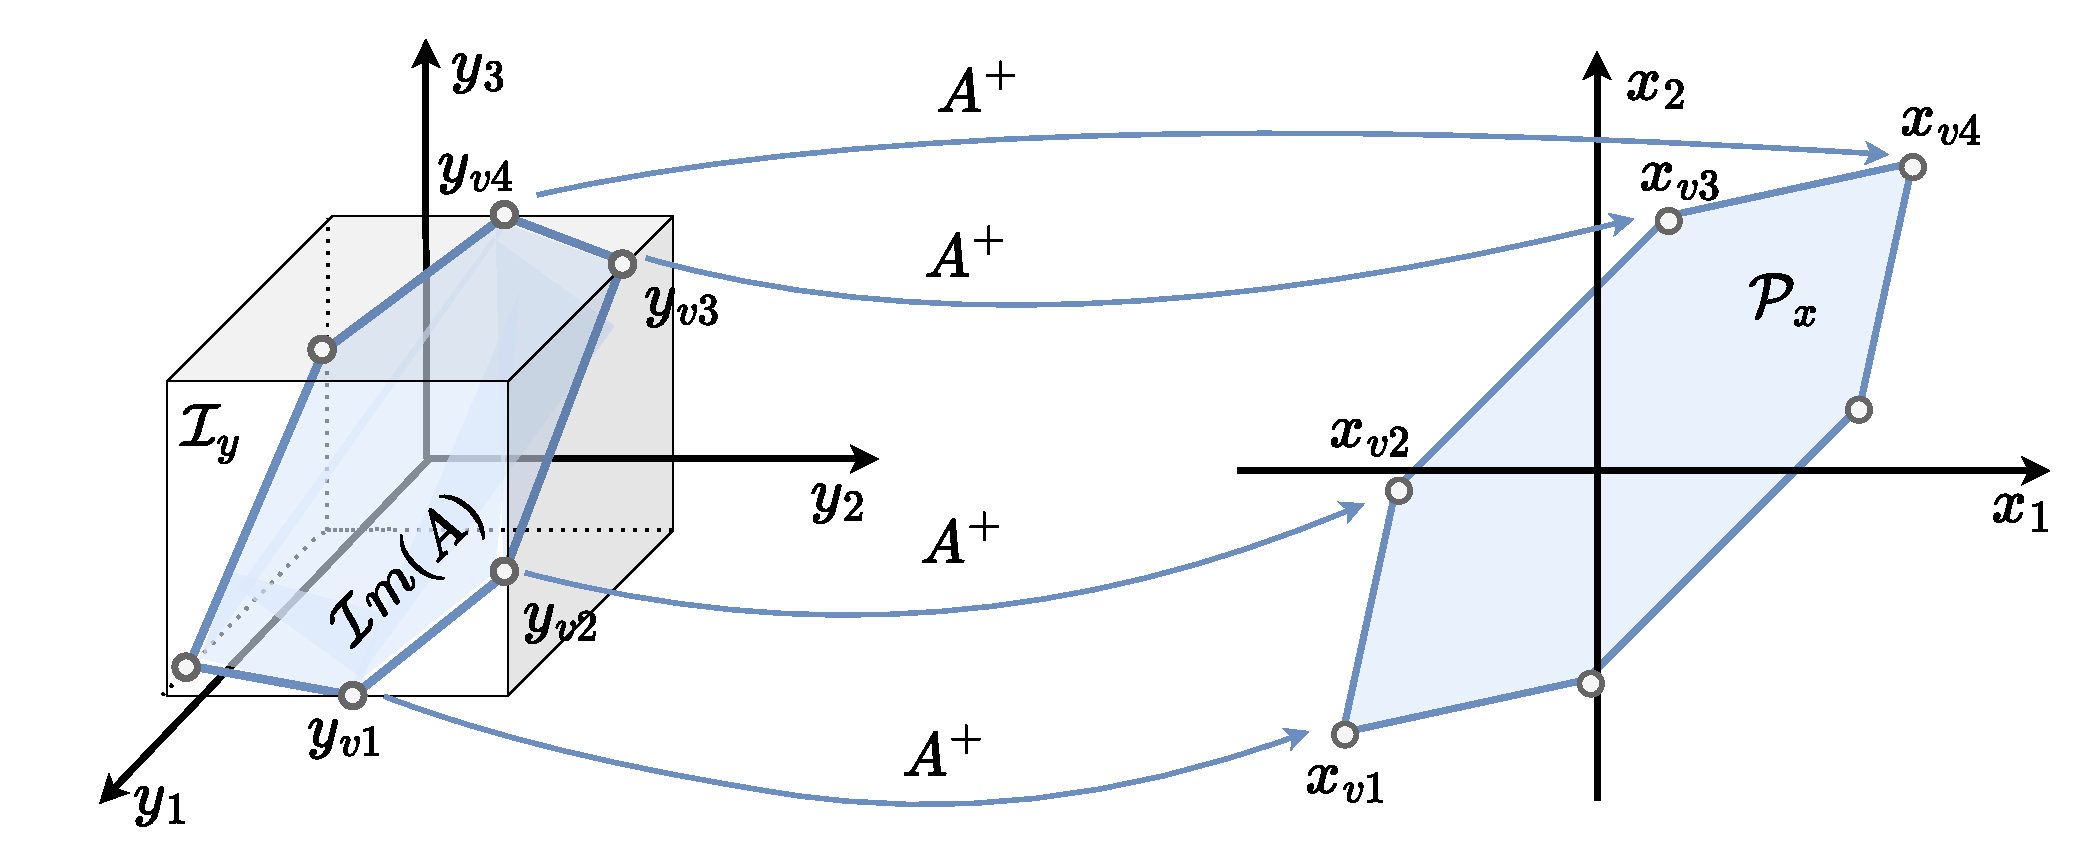
\includegraphics[width=0.8\linewidth]{Papers/images/intersection_algo.pdf}
    \caption{Example intersection polytope $\mathcal{P}_x$ with $n=3$ dimensional interval input set $\mathcal{I}_y$ and $m=2$ dimensional output space. The polytope $\mathcal{P}_x$ vertices $\bm{x}_{vi}$ correspond to the vertices of the intersection $\mathcal{I}_y\cap\img{A}$ denoted as $\bm{y}_{vi}$, through the pseudo-inverse $A^T$ of the matrix $A$.}
    \label{fig:intersection_algo}
\end{figure}

As shown on \Cref{fig:intersection_algo}, the space of all the input vectors $\bm{y}\in\mathbb{R}^n$, bounded within the interval shaped input set $\mathcal{I}_y$, geometrically forms an $n$-dimensional hyperrectangle (orthotope) with $n$ pairs of parallel sides defined by the output limits $\bm{y}\in[\bm{y}_{min},~\bm{y}_{max}]$. The image of the $A$ matrix $\img{A}$ is a $r$-dimensional subspace of the hyperrectangle, where $r$ is the rank of $A$. In  the remainder of this section, the matrix $A$ is, without loss of generality, assumed to be full column rank, i.e. $m$=$r$. 

As discussed in \Cref{ch:inter_formulaiton}, the output space polytope $\mathcal{P}_x$ is the direct affine projection of the intersection between the image $\img{A}$ and the input set $\mathcal{I}_y$ using the pseudo-inverse $A^+$ of the matrix $A$. Therefore this algorithm aims to efficiently find the vertices $\bm{x}_{vi}$ of the polytope $\mathcal{P}_x$, by efficiently finding the vertices $\bm{y}_{vi}$ of the intersection $\mathcal{I}\cap \img{A}$, and project them to the output space using the relationship
\begin{equation}
    \bm{x}_{vi} = A^{+}\bm{y}_{vi}, \qquad \text{where} \quad \bm{y}_{vi}\in\mathcal{I}_y\cap \img{A} \label{eq:compute_vert}
\end{equation}

Therefore the operation of enumerating all the vertices $\bm{x}_{vi}$ of the polytope $\mathcal{P}_x$ can be seen as first finding the $\repr{V}$-representation (the set of vertices $\bm{y}_{vi}$) of the intersection  $\mathcal{I}\cap \img{A}$, followed by its projection to the output space through the pseudo-inverse $A^+$, to obtain the $\repr{V}$-representation of the polytope $\mathcal{P}_x$
\begin{equation}
    \mathcal{P}_x = \conv{A^+\bm{y}_{v1},~A^+\bm{y}_{v1},~\ldots~ }
\end{equation}

\begin{wrapfigure}{r}{0.45\linewidth}
\vspace{-0.5cm}
    \centering
    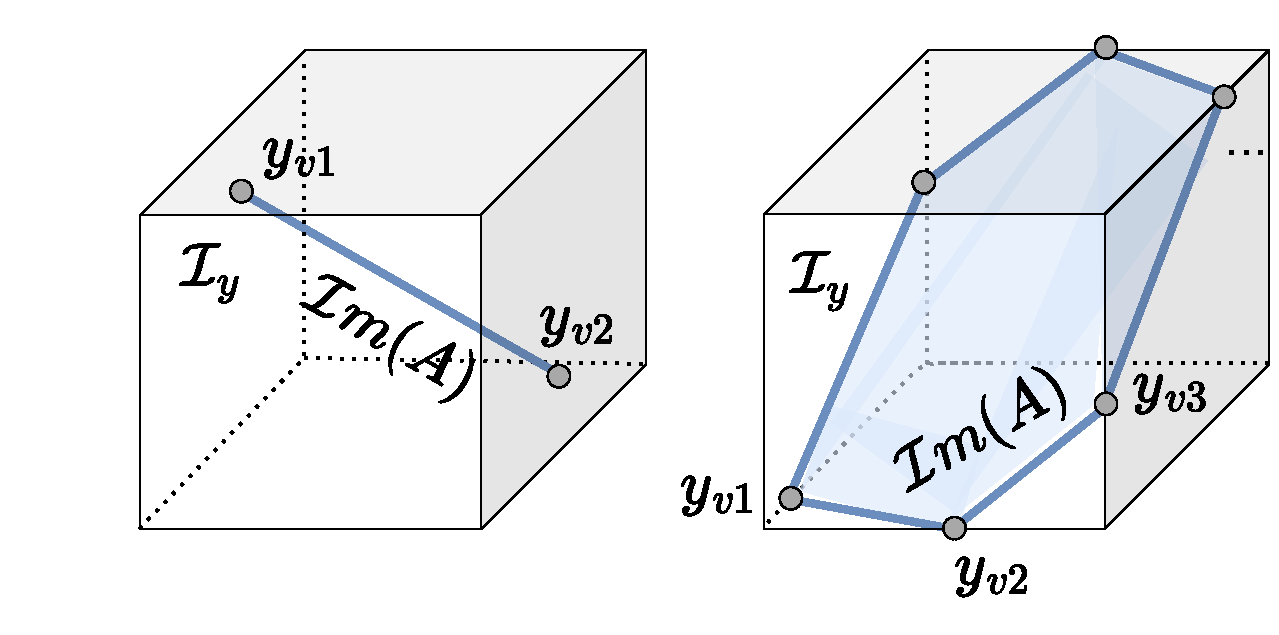
\includegraphics[width=\linewidth]{Papers/images/intersetcion_size.pdf}
    \caption{Example of intersection vertices $\bm{y}_{vi}$ placement on $n\!-\!m$ dimensional faces of hyperrectangle $\mathcal{I}_y$. Left, $m=1$, the vertices $\bm{y}_{vi}$ are on $n\!-\!m\!=\!2$ dimensional faces (sides), while on the right $m=2$ the vertices are on $n\!-\!m\!=\!1$ dimensional faces (edges) }
    \label{fig:size_inter}
\end{wrapfigure}
In their work, \citet{sasaki2011vertex} have shown that, when the input space dimension is $n$ and the image $\img{A}$ dimension is $m$, the extreme values (vertices) of the intersection $\bm{y}_{vi}$ belong to the $n-  m$ dimensional faces of the hyperrectangle $\mathcal{I}_y$. \Cref{fig:size_inter} demonstrates this relationship on an example with the input space dimension $n=3$ and two different output space dimensions $m=1$ and $m=2$. For $m=1$ the vertices $\bm{y}_{vi}$ are on $m-n=2$ dimensional faces of the hyperrectangle corresponding to its sides, and when $m=2$ the vertices  $\bm{y}_{vi}$ are on $m-n=1$ dimensional faces of the hyperrectangle, its edges.

In order to find the  $\repr{V}$-representation of the intersection  $\mathcal{I}\cap \img{A}$, the state-of-the-art algorithms, proposed by \citet{chiacchio_evaluation_1996} and \citet{sasaki2011vertex}, propose an exhaustive search over all the $n$-$m$ dimensional hyperrectangle faces to find the extreme values of $\bm{y}_{vi}$. In this work a new representation of output vector $\bm{y}$ is proposed enabling an efficient navigation of the $n-m$ dimensional hyperrectangle faces. Additionally, an efficient approach to discarding the hyperrectangle faces that cannot contain vertices is integrated in the algorithm, further reducing the complexity of the exhaustive search.

\subsection{Proposed VEPOLI$^2$ algorithm}
Consider an input vector $\bm{y}$ bounded within the input set $\mathcal{I}_y$. It can be defined as
\begin{equation}
    \bm{y} = {\bm{y}}_{min} + \alpha_1 \bm{y}_1+ \alpha_2 \bm{y}_2 + ... + \alpha_n \bm{y}_n
    \label{eq:torque_new}
\end{equation}
where $\alpha_i \in [0,1]$ are scalars weights and vectors $\bm{y}_i$ are orthogonal base vectors in \gls{js}aligned with $i$-th axis of the hyperrectangle $\mathcal{I}_y$, defined as $\bm{y}_i = \begin{bmatrix} 0~\ldots~y_{i,max} - y_{i,min}~\ldots~0 \end{bmatrix}^T$. As shown on the example on \Cref{fig:navigation_y}, the input vector $\bm{y}$ representation (\ref{eq:torque_new}) can be exploited to reach any point within the hyperrectangle $\mathcal{I}_y$, by choosing appropriate scalars $\alpha_i$ in range $[0,1]$. Finding the appropriate values of the scalars $\alpha_i$, for any given $\bm{y}$, can be formulated in a form of linear system
\begin{equation}
\underbrace{\begin{bmatrix}
    \bm{y}_1&\cdots&\bm{y}_n
\end{bmatrix}}_{Y_{n\times n}}\underbrace{\begin{bmatrix}
    \alpha_1\\
    \cdots\\
    \alpha_n
\end{bmatrix}}_{\bm{\alpha}_{n\times 1}} = \bm{y}_{min} - \bm{y}, \qquad  \bm{\alpha} = Y^{-1}(\bm{y}_{min} - \bm{y})
\label{eq:define_Y_Alpha}
\end{equation}
where the matrix $Y$, containing the orthogonal base vectors $\bm{y}_i$, is square and always invertible. 
Furthermore, as the intersection vertices $\bm{y}_{vi}$ belong to the $n$-$m$ dimensional faces of the input hyperrectangle $\mathcal{I}_y$, the representation (\ref{eq:torque_new}) can be further simplified. Any input vector $\bm{y}$, belonging to an $n-m$ dimensional face of the hyperrectangle $\mathcal{I}_y$, can be reached by choosing the appropriate values of $n-m$ scalars $\alpha_i\in[0,1]$, while the other $m$ scalars are fixed to either 0 or 1 ($\alpha_i\in\{0,1\}$).

\begin{figure}
    \centering
    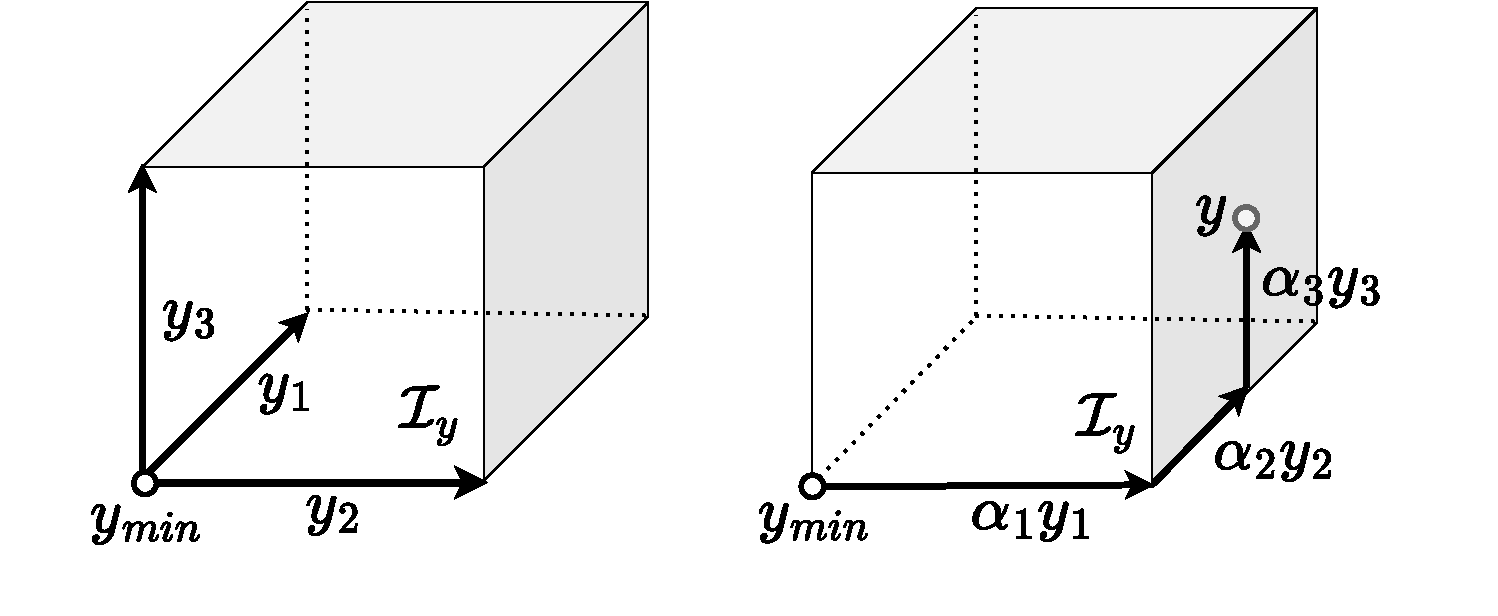
\includegraphics[width=0.6\linewidth]{Papers/images/navigation_y.pdf}
    \caption{Example of the vector representation (\ref{eq:torque_new}) on the $n\!=\!3$ dimensional hyperrectangle $\mathcal{I}_y$. Base vectors $\bm{y}_i$ are shown on the left, and on the right their linear combination using scalars $\alpha_i$ is shown reaching the point $\bm{y}\in\mathcal{I}_y$.}
    \label{fig:navigation_y}
\end{figure}
Furthermore, $n-m$ scalars $\alpha_i\in[0,1]$ can be interpreted as coordinates of the $n-m$ dimensional face, while the remaining $m$ fixed scalars $\alpha_i\in\{0,1\}$, to either 0 or 1, define its origin $\bm{y}_o$
\begin{equation}
    \bm{y}_o = \bm{y}_{min} + \alpha_1 \bm{y}_1+ ... + \alpha_m \bm{y}_m, \qquad \alpha_i \in\{0,1\}
\end{equation} 
Then any $\bm{y}$, belonging to a face of the hyperrectangle, can be expressed using the face's origin $\bm{y}_o$ and its set of $n-m$ scalars $\alpha_i$ 
\begin{equation}
    \bm{y} = \bm{y}_o ~+ ~\alpha_{m+1}\bm{y}_{m+1} +~\cdots~ +\alpha_{n}\bm{y}_{n}, \qquad \alpha_i \in [0,1]
\end{equation}
The vector $\bm{\alpha}\in\mathbb{R}^n$ can be conveniently divided into two components, $\bm{\alpha}_o\in\mathbb{R}^m$ containing $m$ scalars $\alpha_i$ defining the origin of the face and $\bm{\alpha}_x\in\mathbb{R}^{n-m}$ containing $n-m$ scalar coordinates $\alpha_i$ of the face. Additionally, the same can be done with the matrix $Y$, divided in $Y_o\in\mathbb{R}^{n\times m}$ corresponding to $m$ base vectors used to define the origin $\bm{y}_o$, and $Y_x\in\mathbb{R}^{n\times (n-m)}$
 corresponding to the $n\!-\!m$ base vectors $\bm{y}_i$ spanning the face. Then the origin $\bm{y}_o$ and the final vector $\bm{y}$ can be expressed as
 \begin{equation}
    \bm{y}_o = \bm{y}_{min} + Y_o\bm{\alpha}_{o}, \qquad \bm{y} = \bm{y}_o +  Y_x\bm{\alpha}_{x}, \qquad \bm{\alpha}_{o}\in\{\bm{0},\bm{1}\},~~ \bm{\alpha}_{x}\in[\bm{0},\bm{1}]
    \label{eq:matrix_new_y}
\end{equation}
Therefore, in order to find all the vertices $\bm{y}_{vi}$ of the intersection $\mathcal{I}_y\cap\img{A}$, the proposed VEPOLI$^2$ algorithm tests if there exists a point intersection (a vertex) between the $\img{A}$ and every single one of the $n-m$ dimensional faces of the hyperrectangle $\mathcal{I}_y$.

Since all the $\bm{y}$ belonging to the image $\img{A}$ can be expressed as $\bm{y}=A\bm{x}$, this relationship can be further exploited to relate the vertices $\bm{y}_{vi}$ of the intersection $\img{A}\cap\mathcal{I}_y$ and the vertices $\bm{x}_{vi}$ of the final polytope $\mathcal{P}_x$. For each face to be tested, the equations  (\ref{eq:inter_hyp_revisit_algo}) and (\ref{eq:compute_vert}) can be combined
\begin{equation}
    \bm{y}_{vi} = A \bm{x}_{vi} = \bm{y}_{oi} + \alpha_{m+1} \bm{y}_{m+1}+ ~...~ + \alpha_n \bm{y}_n \label{eq:step2}
\end{equation}
where, $\bm{y}_{oi}$ is the origin of the $n\!-\!m$ dimensional face, spanned by the scalar $n\!-\!m$ scalars $\bm{\alpha}_{xi}$. For each face $i$, by fixing the appropriate $m$ scalars $\bm{\alpha}_{oi}$ to 0 or 1, its origin $\bm{y}_{oi}$ can be calculated using (\ref{eq:matrix_new_y}). In order to determine if this face contains the vertex of the intersection $\mathcal{I}_y\cap\img{A}$, a linear system derived from equation~(\ref{eq:step2}) can be solved. This system finds the remaining $n\!-\!m$ scalars $\bm{\alpha}_{xi}$ as well as the corresponding vertex $\bm{x}_{vi}$ at the same time
\begin{equation}
    \underbrace{\begin{bmatrix}A&-\bm{y}_{m+1} \, \dots \, -\bm{y}_{n} \end{bmatrix}}_{Z_{n\times n}} \begin{bmatrix}\bm{x}_{vi}\\ \alpha_{m+1} \\ \vdots\\\alpha_{n} \end{bmatrix} =\begin{bmatrix}A &Y_{xi} \end{bmatrix}\begin{bmatrix}\bm{x}_{vi}\\ \bm{\alpha}_{xi} \end{bmatrix}  = \bm{y}_{oi}, \qquad \begin{bmatrix}\bm{x}_{vi}\\ \bm{\alpha}_{xi} \end{bmatrix} = Z^{-1}\bm{y}_{oi}, 
    \label{eq:linear_system_full}
\end{equation}
Matrix $Z\in\mathbb{R}^{n\times n}$ is a square matrix where each one of the vectors $\bm{y}_i$ is independent. If the matrix $Z$ is singular, geometrically, the image $\img{A}$ is parallel to the face being tested, therefore no intersections exist. If $Z$ is invertible and the $n-m$ scalars $\bm{\alpha}_{xi}$ are obtained, a simple check if $\bm{\alpha}_{xi} \in [\bm{0},\bm{1}]$ can be used to determine if $\bm{x}_{vi}$ is a vertex of the polytope $\mathcal{P}_x$. Geometrically, the condition $\bm{\alpha}_{xi} \in [\bm{0},\bm{1}]$ ensures that the intersection point between the $\img{A}$ and the $n\!-\!m$ dimensional face, is also inside $\mathcal{I}_y$. One of the nice features of this approach is that it does not require an explicit inversion of $A$, as in equation~(\ref{eq:compute_vert}), to obtain the set of vertices composing $\mathcal{P}_x$.

Following three sections bring the approaches further improving the efficiency of the proposed algorithm. First, the dimension of the matrix $Z$ is reduced using the \gls{svd}, then the parallelism of the faces of the hyperrectangle is exported to reduce the number of the computations of the system (\ref{eq:linear_system_full}). Finally, an additional condition is introduced enabling to discard faces and avoid the unnecessary matrix inversions.


\subsubsection{Matrix size reduction using the SVD}

In order to reduce the dimension of the linear system (\ref{eq:linear_system_full}), the \gls{svd} \cite{klema_singular_1980} of $A^T$ is used
\begin{equation}
     A^T =  U  \underbrace{\begin{bmatrix}S & O_{m\times (n-m)}\end{bmatrix}}_{\Sigma}\underbrace{\begin{bmatrix}V_1^T \\ V_2^T \end{bmatrix}}_{V^T}
\end{equation}
where $S= diag( \sigma_1 \dots \sigma_m)$ is a diagonal matrix containing the $m$ singular values of $A^T$. $V_1^T \in \mathbb{R}^{m \times n}$ is the projector from the input space onto the image of $\img{A}$ and $V_2^T \in \mathbb{R}^{n-m \times n}$ is a basis of $\ker{A}$. $V_1^T$ and $V_2^T$ are orthogonal vector subspaces yielding $V_2^T V_1 = 0$ and thus 
\begin{equation}
    V_2^T A\bm{x} = \bm{0}
\end{equation}
Then, multiplying the equation (\ref{eq:linear_system_full}) with $V^T_2$
\begin{equation}
    V_2^T\begin{bmatrix}A &Y_{xi} \end{bmatrix}\begin{bmatrix}\bm{x}_{vi}\\ \bm{\alpha}_{xi} \end{bmatrix}  = \underbrace{V_2^TA\bm{x}_{vi}}_{\bm{0}} + V_2^TY_{xi}\bm{\alpha}_{xi} = V_2^T\bm{y}_{oi} 
\end{equation}
allows to reduce the system (\ref{eq:linear_system_full}) to
\begin{equation}
    \underbrace{V_2^T\begin{bmatrix}-\bm{y}_{m+1} ~\dots~ -\bm{y}_{n} \end{bmatrix}}_{T_{(n-m)\times (n-m)}} \bm{\alpha}_x  = V_2^TY_{xi}\bm{\alpha}_{xi} = V_2^T\bm{y}_{oi}
    \label{eq:linear_system_svd}
\end{equation}
If $T$ is invertible, $\bm{\alpha}_{xi}$ can be computed by
\begin{equation}
\bm{\alpha}_{xi} = T^{-1}V_2^T\bm{y}_{oi}
\label{eq:svd_linear_sys_step1}
\end{equation}
When the computed $\bm{\alpha}_{xi}$ complies with the check $\bm{\alpha}_{xi} \in [\bm{0},\bm{1}]$,  the corresponding polytope vertex can be calculated as
\begin{equation}
    \bm{x}_{vi} = A^{+} \big( \bm{y}_{oi} + Y_{xi}\bm{\alpha}_{xi}\big)
\label{eq:svd_linear_sys_step2}
\end{equation}

This new approach requires the calculation of the \gls{svd} and the pseudo-inverse $A^{+}$. Nevertheless, since the pseudo-inverse can be efficiently calculated from the \gls{svd} as $A^{+} = U\Sigma^{T+}V^T$ and since both the \gls{svd} and pseudo-inverse are calculated once per algorithm run, the computation efficiency is greatly improved due to the matrix dimension reduction from $n$ to $(n-m)$ when inverting $T$ instead of $Z$.

\begin{figure}[!t]
    \centering
    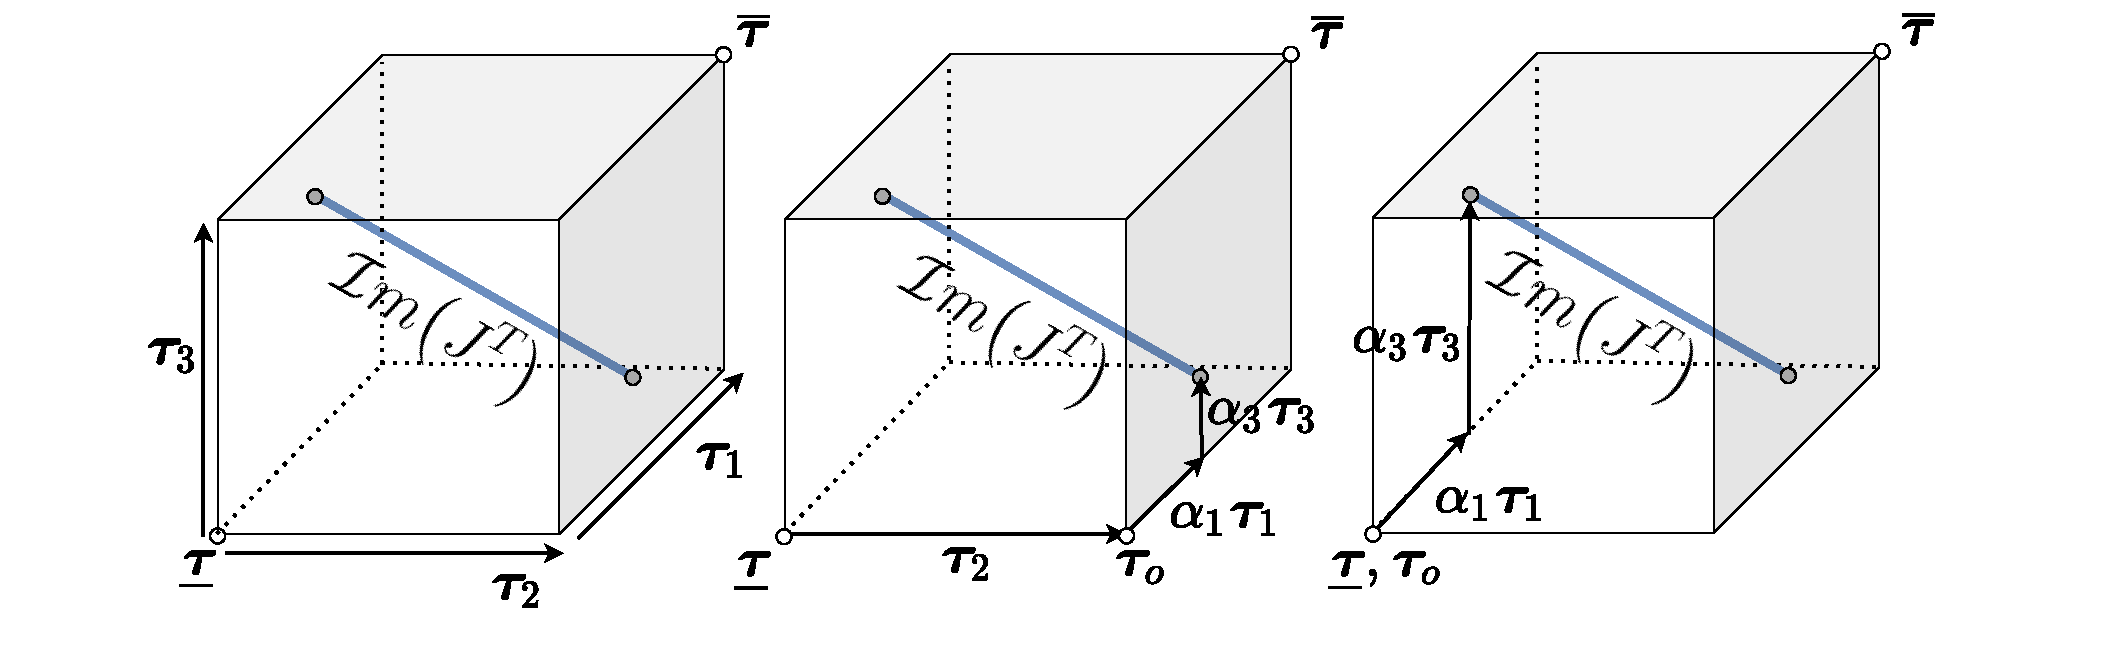
\includegraphics[width=0.9\linewidth]{Papers/images/intersection_example.pdf}
    \caption{Example of input space interpretation of the VEPOLI$^2$ algorithm for the system $n$=$3$ and $m$=$1$. The two vertices of the intersection $\{\bm{y}_{v1},\bm{y}_{v2}\}$ are reached by solving the linear system (\ref{eq:linear_system_full}) or (\ref{eq:linear_system_svd}). The vertices belong to the parallel ($n\!-\!m\!=\!2$ dimensional faces) sides of the hyperrectangle $\mathcal{I}_y$.  }
    \label{fig:intersection_example}
\end{figure}

\begin{wrapfigure}[12]{r}{0.25\linewidth}
\vspace{-0.5cm}
    \centering
    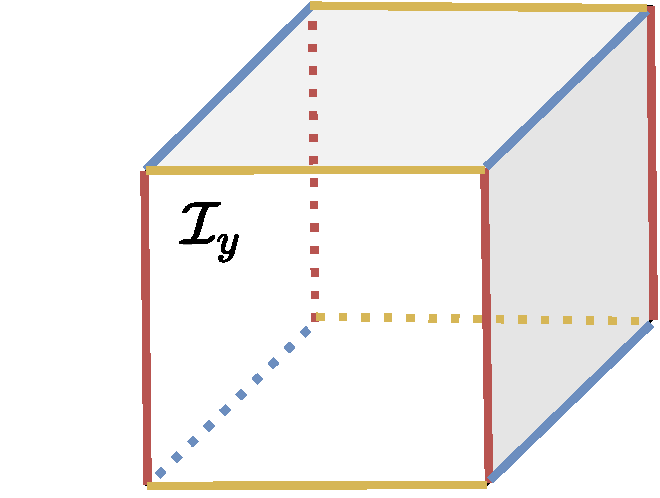
\includegraphics[trim=1.5cm 0 0 0,clip=true,width=\linewidth]{Papers/images/parallel.pdf}
    \caption{All the parallel edges of the 3D hyperrectangle shown in differing colours. It has 3 (red, blue, yellow) sets of 4 parallel edges, 12 edges in total.}
    \label{fig:parallel}
\end{wrapfigure}
\subsubsection{Exploiting the parallelism of the hyperrectangle faces} 
The number of $n-m$ dimensional faces of an $n$ dimensional hyperrectangle $\mathcal{I}_y$ can be calculated using the expression
$$
N_{n,(n-m)}= 2^{n-(n-m)}\binom{n}{n-m} =  2^{m}\binom{n}{m} 
$$
More precisely, an $n$ dimensional hyperrectangle has $\big(\begin{smallmatrix}n\\m\end{smallmatrix}\big)$ sets of $2^m$ parallel faces with the dimension $n\!-\!m$. 
As illustrated on \Cref{fig:parallel}, a 3D ($n\!=\!3$) hyperrectangle has $\big(\begin{smallmatrix}3\\1\end{smallmatrix}\big)\!=\!3$ sets of $2^{2}\!=\!4$ parallel ($n\!-\!m\!=\!1$) edges, as well as $\big(\begin{smallmatrix}3\\2\end{smallmatrix}\big)=3$ sets of $2^1\!=\!2$ parallel ($n\!-\!m\!=\!2$) sides. 

All the parallel $n\!-\!m$ dimensional faces of the hyperrectangle $\mathcal{I}_y$ can be spanned using the same set of $n\!-\!m$ scalars $\bm{\alpha}_{xi}$, while the remaining $m$ scalars $\bm{\alpha}_{oi}$ can be used to find their $2^m$ origins $\bm{y}_{oi}$.

\Cref{fig:intersection_example} illustrates the case where $\img{A}$ is a line ($m=1$) and the input space is $n=3$ dimensional. In this case the intersection vertices $\{\bm{y}_{v1},\bm{y}_{v2}\}$ lie in $n$-$m$=$2$ dimensional hyperrectangle faces. In that example, both vertices $\bm{y}_{vi}$ are placed on two parallel faces, spanned by the two scalars $\alpha_1$ and $\alpha_3$, while the scalar $\alpha_2$, set to $0$ or $1$, is used to find their origins $\bm{y}_{oi}$.

In the linear system (\ref{eq:linear_system_svd}), matrix $T$ has the same content for each parallel face of the hyperrectangle. Therefore, the inverse $T^{-1}$ can be recalculated only once per set of parallel faces. Then, for each of the $2^m$ parallel faces within the set, the vertex $\bm{x}_{vi}$ and the corresponding $\bm{\alpha}_{xi}$, can be obtained by multiplying the $2^n$ origins $\bm{y}_{oi}$ with $T^{-1}$, as described by (\ref{eq:svd_linear_sys_step1}-\ref{eq:svd_linear_sys_step2}).

Overall, in order to test all possible combinations of the $n\!-\!m$ dimensional faces which may contain vertices of the intersection (and in term the final polytope $\mathcal{P}_x$), the total of $\big(\begin{smallmatrix}n\\m\end{smallmatrix}\big)$=$\frac{n!}{m!(n-m)!}$ inversions of the matrix $T$ and  $2^m\big(\begin{smallmatrix}n\\m\end{smallmatrix}\big)$ checks $\bm{\alpha}_{xi} \in [\bm{0},\bm{1}]$ have to be performed.

In the case depicted in \Cref{fig:intersection_example} ($n$=$3$, $m$=$1$), $T$ is inverted only $\big(\begin{smallmatrix}3\\1\end{smallmatrix}\big)$=$3$ times and conditions are evaluated 6 times, which corresponds exactly to the number of sides of the hyperrectangle. In the same example, if the output space would be 2D ($n$=$3$, $m$=$2$) the number of $T$ inversions is 3 and the number of condition evaluation is 12, which corresponds to the number of edges of the hyperrectangle. 

\subsubsection{Matrix inverse condition} 

The most time consuming aspect of the proposed VEPOLI$^2$ algorithm is the relatively high number of matrix $T$ inversions. Therefore this section proposes a necessary condition to discard the sets of faces that cannot contain a vertex and avoid unnecessary matrix $T$ inversions.

\begin{wrapfigure}{r}{0.35\linewidth}
    \centering
    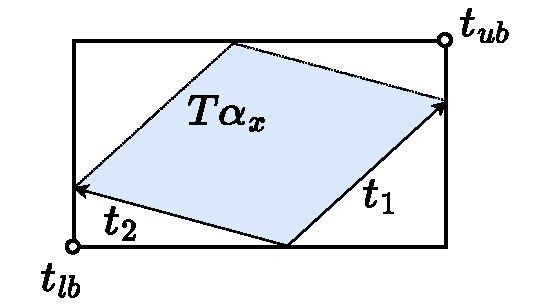
\includegraphics[width=\linewidth]{Papers/images/matrix_condition.pdf}
    \caption{The bounding-box calculated using the equation (\ref{eq:bounds_condition}). The size of the example system is $n\!-\!m\!=\!2$, where $\bm{t}_1,\bm{t}_2$ are column vectors of the matrix $T$.}
    \label{fig:matrix_condition}
\end{wrapfigure}
Due to the constrained nature of the scalars $\bm{\alpha}_{xi}\in[\bm{0},\bm{1}]$, it is possible to efficiently calculate the bounds (${\bm{t}_{ub}}$ and $\bm{t}_{lb}$) on the $T\bm{\alpha}_{xi}$ 
\begin{equation}
    T\bm{\alpha}_{xi}  \in [\bm{t}_{lb}, \bm{t}_{ub}]\label{eq:necesassry_condition1}
\end{equation}
As the column vectors $\bm{t}_i$ within the matrix $T$ are, in the general case not orthogonal, the min-max interval shaped set can not exactly characterise the feasible set of $T\bm{\alpha}_{xi}$. However, an interval that over-approximates it, can be found very efficiently by row-wise summing only positive and only negative elements $t_{ij}$ of  $T$
\begin{equation}
t_{i,lb} = \sum_j \max(t_{ij}, 0), \qquad
t_{i,lb} = \sum_j \min(t_{ij}, 0) 
\label{eq:bounds_condition}
\end{equation}
As shown on \Cref{fig:matrix_condition}, this creates a bounding box around the space defined by  $T\bm{\alpha}_{xi}$.

In order for the system (\ref{eq:linear_system_svd}) to have a solution, the null-space projections of the vectors $\bm{y}_{oi}$ have to respect the same bounds as well
\begin{equation}
    V_2^T\bm{y}_{oi} \in [\bm{t}_{lb}, \bm{t}_{ub}]\label{eq:necesassry_condition}
\end{equation}
Therefore, using this bounding box, the necessary check can be devised for the inversion of the matrix $T$. If all the $2^m$ combinations of $V_2^T\bm{y}_{oi} \notin [\bm{t}_{lb}, \bm{t}_{ub}] $, the system (\ref{eq:linear_system_svd}) cannot have a solution which satisfies $\bm{\alpha}_{xi} \in [\bm{0},\bm{1}]$, and there is no need to invert $T$ to figure it out.

The condition $V_2^T\bm{y}_{oi} \in [\bm{t}_{lb}, \bm{t}_{ub}] $ is a necessary condition, however as the interval $[\bm{t}_{lb}, \bm{t}_{ub}]$ presents an over-approximation of the achievable set $T\bm{\alpha}_x, \bm{\alpha}_x\in[\bm{0}, \bm{1}]$, it is not a sufficient condidion. 

The bounding box (\ref{eq:bounds_condition}), as well as the $2^m$ face origins $\bm{y}_{oi}$ can be calculated efficiently, allowing for a computationally inexpensive reduction in the number of matrix inversions. The upper bound on the number of matrix inversions $N_{inv}$ can be found by studying the worst-case scenario, where all the origins $\bm{y}_{oi}$ pass the condition (\ref{eq:necesassry_condition}). In this case the number of inversion corresponds to the binomial $\binom{n}{m}$. In the general case, the number of matrix inversions $N_i$ is bounded and equals to  
$$N_{inv}\leq\binom{n}{m}=\frac{n!}{m!(n-m)!}$$
The number of checks $N_c$ of the condition $\bm{\alpha}_{xi} \in [\bm{0},\bm{1}]$, per matrix inversion, is bounded as well, as the origin vectors $\bm{y}_{oi}$ that do not comply with the necessary condition (\ref{eq:necesassry_condition}) can be discarded from the these checks as well
$$
N_c\leq2^m
$$

\subsection{Performance and complexity comparison}\label{sec:complexity}
To demonstrate the efficiency of the VEPOLI$^2$ algorithm, it is compared against the polytope vertex search algorithm introduced by \citet{chiacchio_evaluation_1996}. Furthermore the comparison is extended to the algorithm proposed by \citet{sasaki2011vertex} which is, to our knowledge, the only algorithm exploiting the geometric structure of the intersection formulation polytope with interval limits (\ref{eq:inter_hyp_revisit_algo}).

\begin{table}[!h]
    \centering
    \begin{tabular}{|c|c|c|c|}
       \hline
      \textbf{ System size }& \textbf{Chiacchio}\cite{chiacchio_evaluation_1996} & \textbf{Sasaki} \cite{sasaki2011vertex}  &  \textbf{VEPOLI$^2$} \\
       \hline
       $(n,m)$& matrix inversions: $ \frac{2n!}{m!(2n-m)!}$  & $ \frac{n!}{m!(n-m)!} $ & $ \leq \frac{n!}{m!(n-m)!}$ \\
       &  matrix size:  $ 2n \times 2n$ & $m\times m$  & $n$-$m$ $\times$ $n$-$m$\\
       & time[ms]: mean $\pm$ std (max) & & \\
       \hline
       $(4,2)$ &  24 & 6 & 4.2$\pm$1.4 (6) \\ 
       & 8$\times$8 & 2$\times$2 & 2$\times$2 \\ 
       & 2.7$\pm$0.1 (3.6) & 0.93$\pm$0.1 (1.1) & 0.64$\pm$0.1 (1.5) \\ 
       \hline
       $(4,3)$ &  32 & 4 & 2.9$\pm$1.1 (4) \\ 
       & 8$\times$8 & 3$\times$3 & 1$\times$1 \\ 
       & 3.7$\pm$0.3 (6.0) & 0.79$\pm$0.08 (1.4) & 0.54$\pm$0.1 (1.4) \\ 
       \hline
       $(6,3)$ & 220 & 20 & 2.8$\pm$2.5 (10) \\ 
        & 12$\times$12 & 3$\times$3 & 3$\times$3 \\ 
       & 14.2$\pm$0.9 (20) & 2.1$\pm$0.2 (3.4) & 1.5$\pm$0.2 (2.7) \\ 
       \hline
      $(6,6)$&   64 & 1 & 1$\pm$0 (1)\\
        &  12$\times$12 & 6$\times$6 & 6$\times6$\\
       & 34.7$\pm$1 (44.3) & 0.32$\pm$0.07 (0.56) & 0.24$\pm$0.04 (0.46)\\
       \hline
      $(7,3)$&    364 & 35 & 7.3$\pm$4.2 (20)\\
        & 14$\times$14 & 3$\times$3 & 4$\times4$\\
       & 25$\pm$0.5 (27) & 3.5$\pm$0.1 (5.4) & 2.6$\pm$0.2 (4.3)\\
       \hline
      $(7,6)$& 448 & 7 & 6.4$\pm$1 (7)\\
        & 14$\times$14 & 6$\times$6 & 1$\times$1\\
       & 150$\pm$34 (360) & 1.6$\pm$0.5 (4) & 1.2$\pm$0.3 (3.0)\\
       \hline
    \end{tabular}
    \caption{Complexity and execution time (in milliseconds) comparison for three different vertex search algorithms. The comparison provided for the number of matrix inversions, matrix size and time of execution, averaged over 1000 random systems. }
    \label{tab:complexity_results}
\end{table}

The three algorithms have been tested on finding the $\repr{V}$-representation of the three different systems, inspired by the wrench ($\bm{f}\in\mathbb{R}^m$) polytope $\mathcal{P}_f$ enumeration for three different robots: a 4R planar robot ($n$=$4$), the {Universal Robots} UR5 6DoF robot ($n$=$6$) and the {Franka Emika Panda} 7DOF robot ($n$=$7$). The planar 4R robot is used to calculate its planar force ($m=2$) and its planar wrench ($m=3$) polytope, while UR5 and Panda are used to calculate \gls{cs} force ($m=3$) and wrench ($m=6$) polytopes. The results are averaged over 1000 randomly generated matrices $A$ and input sets $\mathcal{I}_y$. All algorithms have been implemented in the programming language Matlab and tested on a laptop equipped with a 1.90GHz Intel i7-8650U processor. The source code of the experiment is publicly available on GitLab\footnote{Gitlab: \url{https://gitlab.inria.fr/auctus-team/people/antunskuric/papers/polytope_vertex_search}}.

\Cref{tab:complexity_results} shows the results of this complexity evaluation. The VEPOLI$^2$ algorithm substantially reduces the number of matrix inversions and thus reduces the processing time considerably: $4$-$10\times$ faster execution than Chiacchio's algorithm and on average 30\% faster than Sasaki's. Results show that, even for the generic cases that correspond to the 6DOF ($n=6$) and 7DOF ($n=7$) industrial robots, the VEPOLI$^2$ algorithm is capable of evaluating both force ($m=3$) and wrench ($m=6$) polytope vertices under $3ms$. Such a low processing time opens numerous opportunities for the online use of polytope based capacity, evaluation especially in the area of robot control. 

\Cref{fig:panda_ur5_force} shows the visualisation of the \gls{cs} force ($m=3$) polytope for the UR5 and Panda robots. Both polytopes are calculated using the VEPOLI$^2$ algorithm.

\begin{figure}
    \centering
    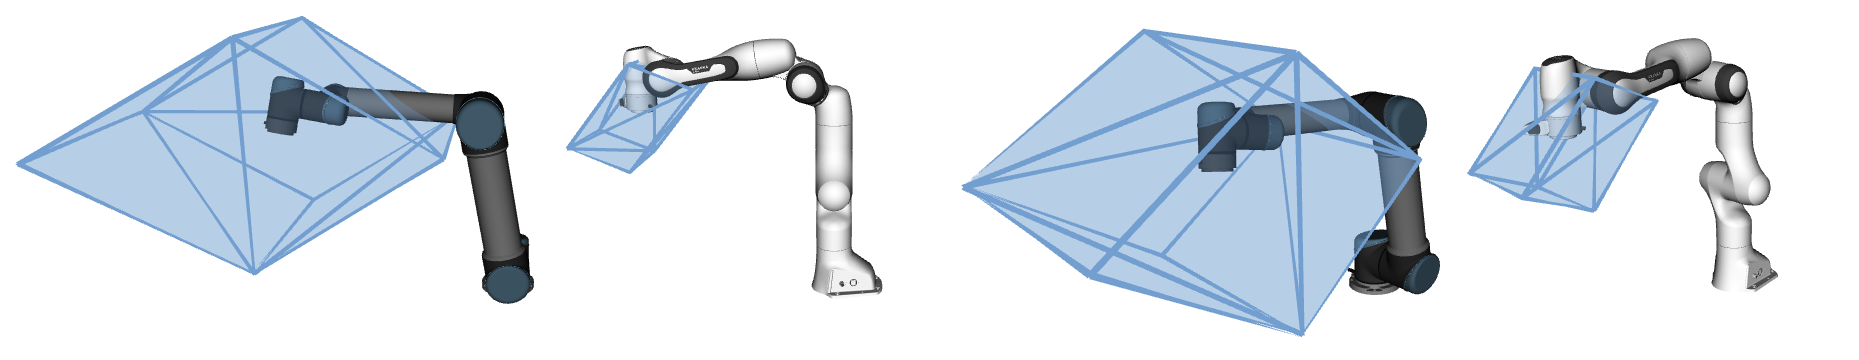
\includegraphics[width=\linewidth]{Papers/images/panda_ur5.png}
    \caption{Two different views of Panda ($n=7$) and UR5 ($n=6$) robot's force polytope ($m=3$) calculated using the VEPOLI$^2$ algorithm. Both robots and polytopes are shown in the same scale (1m : 1000N). The figure shows that the UR5 has much larger polytope than Panda robot. This is due to its larger force capacity, as UR5 is rated for 5kg loads whereas Panda is rated for 3kg loads.}
    \label{fig:panda_ur5_force}
\end{figure}

\subsection{Discussion on limitations}
This algorithm, being based on the algorithm proposed by \citet{sasaki2011vertex}, is still based on the exhaustive search. Even though significantly reducing the complexity of the Sasaki's method, it is not particularly well suited for high dimensions $n$ of the input space, especially if the difference between the input and the output space dimension $n\!-\!m$ is large. 

The algorithm has two computational bottlenecks: the number of matrix $T$ inversions $N_{inv}$ and the number of checks $\bm{\alpha}_{xi} \in [\bm{0},\bm{1}]$ per matrix inversion $N_c$.

If the system has high dimensional input space and low dimensional output space ($n\gg m$) then the number of matrix inversions $N_{inv}=\binom{n}{m}$ will be large, while the number of checks $N_c=2^m$  will be low. 
On the other hand, if the system has both high dimensional input space and high dimensional output space ($n\approx m$ and $n,m\gg0$), then the number of matrix inversions $N_{inv}=\binom{n}{m}$ will be relatively low and will not be the limiting factor, but the number of checks $N_c=2^m$ which will be very high. Therefore, although the algorithm is created in a generic form and can find the $\repr{V}$-representation of any polytope belonging to this family, it is particularly efficient when the dimensions of the input and the output space are relatively low. 

Furthermore, as the VEPOLI$^2$ algorithm exploits the null-space $\ker{A}$ of the matrix $A$ to gain on efficiency, it is not suitable for the systems where the matrix $A$ is square ($m\!=\!n$), as in that case the null-space does not exist $\ker{A}=\{\varnothing\}$. However, as discussed in the \Cref{par:equivalent_proj}, this specific case of interval projection is much easier to work with as it corresponds to the projection formulation, which $\repr{V}$-representation can be determined in a straight-forward manner, as described in \Cref{ch:proj_algos_v}, by projecting the vertices of the hyperrectangle to the output space.


\begin{algorithm}[!t]
\caption{The VEPOLI$^2$ algorithm pseudo-code}
\begin{algorithmic}
\REQUIRE $A$, $\bm{y}_{min}$, $\bm{y}_{max}$ (Eq. \ref{eq:interval_revisit_algo}) 
\STATE $U, \Sigma, V^T \leftarrow svd(A^T)$ 
\STATE $A^{+} = U\Sigma^{T+}V^T$
\STATE $V_1,\, V_2  \leftarrow V $
\STATE calculate $n$ base vectors $\bm{y}_1 \dotsc \bm{y}_n$ (Eq. \ref{eq:torque_new})

\STATE init $\repr{V}$-rep: $X_v$, $Y_v$ $\!\leftarrow\! []$

\FORALL{  $\big(\begin{smallmatrix}n\\m\end{smallmatrix}\big)$ combinations of $m$ fixed $\alpha_i$ } 
\STATE construct matrices $Y_o$ and $Y_x$
\STATE $T = V_2^TY_x$
\IF{matrix T invertible}
\STATE find bounds $\bm{t}_{lb},\bm{t}_{ub}$ (Eq. \ref{eq:bounds_condition})
\STATE init list of origins $\bm{y}_o$ satisfying the condition (Eq. \ref{eq:necesassry_condition}): $L_o$ $\!\leftarrow\! []$ 
\FORALL{   $2^m$ vectors $\bm{\alpha}_o$ }
\STATE $\bm{y}_o = \bm{y}_{min} +  Y_o\bm{\alpha}_o$ 
\IF{$ V_2^T\bm{y}_o \in [\bm{t}_{lb},\bm{t}_{ub}] $}
\STATE update candidates: $L_o \!\leftarrow\! [L_o,~ \bm{y}_o]$
\ENDIF
\ENDFOR

\IF{$L_o$ not empty}
\STATE calculate the inverse $T^{-1}$
\FORALL{   $\bm{y}_o$ in $L_o$ }
\STATE $\bm{\alpha}_x = T^{-1}V_2^T\bm{y}_o $
\IF{$ \bm{\alpha}_x \in [\bm{0},\bm{1}] $}
\STATE $\bm{y}_{v} = \bm{y}_o + Y_x\bm{\alpha}_x$ 
\STATE $\bm{x}_{v} = A^{+}\bm{y}_{v}$ 
\STATE update $\repr{V}$-rep: ${X}_{v} \!\leftarrow\! [{X}_{v},~ \bm{x}_v ]$, ${Y}_{v} \!\leftarrow\! [{Y}_{v},~ \bm{y}_v ]$ 
\ENDIF
\ENDFOR
\ENDIF


\ENDIF

\ENDFOR
\RETURN $\repr{V}$-rep: $X_v$, $Y_v$

\end{algorithmic}
\label{alg:algo_1}
\end{algorithm}

\subsection{Algorithm implementation}
\qrimg{qrcodes/pycapacity.png}{https://auctus-team.github.io/pycapacity/}{\codet{pycapacity}}
The pseudo-code of the proposed algorithm is given in \Cref{alg:algo_1}, while an efficient open-source Python implementation is publicly available within the package \codet{pycapacity}\footnote{\href{https://auctus-team.github.io/pycapacity/}{https://auctus-team.github.io/pycapacity/}}, which is described more in detail in \Cref{ch:software}.\\\\
\Cref{ch:robot_robot_carrying} brings the application of the VEPOLI$^2$ algorithm for the real-time robot control in the human-robot collaboration scenario, where the algorithm is exploited in order to calculate the robot's wrench capacity polytope online. 



\section{ICHM: New algorithm for polytope approximation}
\label{ch:algorihtm_ichm}

This section introduces a new polytope approximation algorithm called \textbf{I}mplicit (or \textbf{I}terative) \textbf{C}onvex-\textbf{H}ull \textbf{M}ethod (ICHM). This algorithm is based \gls{chm}, developed by \citet{lassez1992quantifier}, and tailored specifically for the generic (implicit) polytope formulation 
\begin{equation}
    \mathcal{P}_x = \big\{ \bm{x}\in \mathbb{R}^{m}\, |\,A\bm{x} = B\bm{y} + \bm{b}, \quad  \bm{y}\in\mathcal{P}_y  \big\}
    \label{eq:generic_polyt_view_revisit2}
\end{equation}
where the input set $\mathcal{P}_y$ can be expressed with its $\repr{H}$-representation
\begin{equation}
    \mathcal{P}_y = \big\{ \bm{y}\in \mathbb{R}^{n}\, |\,H_y\bm{y} \leq \bm{d_y}\big\}
    \label{eq:generic_poly_input_set_revisit2}
\end{equation} 
This polytope formulation, as discussed in \Cref{ch:collab_metrics_overview}, unifies the formulations of all the common polytope characterisations of human's and robot's physical abilities. The correspondence of different physical ability polytopes and the formulation (\ref{eq:generic_polyt_view_revisit2}) can be found in \Cref{tab:merged_table}. 

The generic polytope formulation (\ref{eq:generic_polyt_view_revisit2}) has an implicit form $A\bm{x}=B\bm{y}$ which cannot be used directly with standard polytope transformation strategies described in \Cref{ch:polytope_algorithms}. More specifically, its formulation corresponds to the intersection-projection, introduced in \Cref{ch:inter_proj_form}, a special case of the intersection formulation 
\begin{equation}
    \mathcal{P}_x \in \{\bm{x}\in \mathbb{R}^m~|~A \bm{x} = \bm{z} + \bm{b},~ \bm{z} \in \mathcal{P}_z\} 
\end{equation}
where the input set polytope $\mathcal{P}_z\in\mathbb{R}^k$ is defined using the projection formulation
\begin{equation}
    \mathcal{P}_z \in \{\bm{z}\in \mathbb{R}^k~|~z = B\bm{y},~ \bm{y} \in \mathcal{P}_y\} 
\end{equation}
Finding the $\repr{V}$ and $\repr{H}$-representation of the polytope $\mathcal{P}_x$, using the standard methods, requires separating the problem and first transforming the input set $\mathcal{P}_z$ in a suitable representation (usually $\repr{H}$), followed by the second step of transforming the final polytope $\mathcal{P}_x$. 

However, when the input space is high dimensional $n\gg1$, both polytope $\mathcal{P}_z$ and $\mathcal{P}_x$ have complex geometries, consisting in large number of vertices and faces. The high dimensional input space (and low dimensional output spaces $n\gg m$) are very common when it comes to characterising the physical abilities of humans, based on their musculoskeletal modes. The musculoskeletal models often have large number of muscles $n\gg1$, often more than 50, while the output space usually corresponds to the 3D \gls{cs} ($m=3$). In such cases, the exact polytope transformation methods have intractable computation times, as they relay on the exhaustive search in the high dimensional input space.

To overcome the complexity of the exhaustive search, various approximate approaches, such as the \gls{rsm}  \cite{agarwal1993ray} and the \glsxtrfull{chm} \cite{lassez1992quantifier} described in \Cref{ch:approximation_algos}, have been developed, reducing the computation complexity and improving the execution time. 
Although \gls{rsm} algorithms are relatively simple to setup they do not provide any bound on their estimation error and highly rely on hand tuned initial parameters. 
\gls{chm} \cite{lassez1992quantifier} algorithms on the other hand, perform a very efficient iterative approximation,  while at the same time guaranteeing the bound of the user defined approximation error. In each iteration \gls{chm} refines the approximation, by using \glspl{lp} to find new vertices of the polytope and Convex-Hull to group them to faces. Furthermore, \gls{chm} finds the $\repr{V}$ and the $\repr{H}$-representation of the polytope at the same time. However in its standard formulation, the \gls{chm} is not suitable for the family of problems given with equation (\ref{eq:generic_polyt_view_revisit2}). 

Therefore, this section proposes a new algorithm extending the \gls{chm} algorithm to the generic polytope formulation (\ref{eq:generic_polyt_view_revisit2}). \Cref{ch:lp_adapt} introduces the \gls{lp} formulation adapting the \gls{chm} approach to the implicit problem formulation (\ref{eq:generic_polyt_view_revisit2}), while \Cref{ch:method} brings the ICHM algorithm overview, as well as the pseudo-code and the geometrical representation. Finally, \Cref{ch:chm_performance} brings the performance analysis of the ICHM and comparison to the state-of-the-art methods on the example of finding the $\repr{V}$-representation of the human wrench capacity polytope based on the musculoskeletal models, which is particularly challenging both due its implicit formulation and high dimensional input space $n\gg m$.

\begin{wrapfigure}[12]{r}{0.32\linewidth}
% \begin{wrapfigure}{r}{0.32\linewidth}
\vspace{-1.5cm}
    \centering
    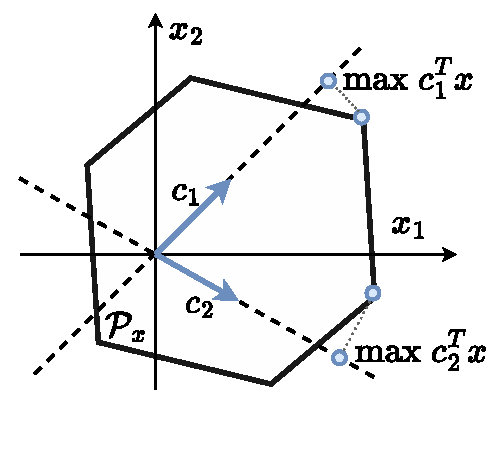
\includegraphics[width=\linewidth]{Papers/images/lp_explication.pdf}
    \caption{The figure demonstrates the \gls{lp} based vertex search by choosing two different vectors $\bm{c}$.}
    \label{fig:lp_explication}
\end{wrapfigure}
\subsection{Linear programming formulation}
\label{ch:lp_adapt}

From a geometrical point of view, solving a \gls{lp} problem boils down to finding a vertex of a polytope \cite{vajda_gass_1964}. 
\begin{equation}
\begin{aligned}
    \bm{x}_v = \text{arg}\max_{\bm{x}} \quad &  \bm{c}^T\bm{x} \\
     \textrm{s.t.} ~~&\bm{x} \in \mathcal{P}_x \\
\end{aligned}
\label{eq:lin_prog_generic}
\end{equation}
However, in order for the polytope $\mathcal{P}_x$ to be suitable for \gls{lp} optimisation in the $m$-dimensional output space, its implicit formulation $A\bm{x}=B\bm{y}$ needs to be expressed in explicit form.

In the general case, the input space is higher dimensional $n\geq m$ and the matrix $A$ is not square. As discussed in \Cref{par:equivalent_proj}, to find an explicit form of equation (\ref{eq:generic_polyt_view_revisit2}), the pseudo-inverse $A^+$ can be used as a solution only if $B\bm{y}+\bm{b}$ belongs to the image $\img{A}$ of $A$ \cite{klema_singular_1980}. Therefore, equation 
\begin{equation}
    A\bm{x} = B\bm{y} + \bm{b}
\end{equation} 
can be transformed to 
\begin{equation}
    \bm{x} = A^{+} (B \bm{y} + \bm{b}), \qquad \text{where} \quad B\bm{y} + \bm{b} \in \mathcal{I}m(A)
    \label{eq:eq_general_red}
\end{equation} 

Using the \gls{svd} \cite{klema_singular_1980} of the matrix $A^T$ produces $A^T = U\Sigma V^T$. The rotation matrix $V \in \mathbb{R}^{n\times n }$ is separated into  $V_1\in \mathbb{R}^{n\times m}$, a projector to the image $\img{A}$ of $A$, and $V_2\in \mathbb{R}^{n\times(n-m)}$, a projector to its null-space $\ker{A}$. As all the vectors belonging to the $\img{A}$ have zero projection to the null-space $\ker{A}$, an equality constraint can be devised for $B\bm{y}+\bm{b}$ to belong to the image $\img{A}$ of $A$. 
\begin{equation}
    V_2^TB\bm{y} +V_2^T\bm{b}  = \bm{0}
    \label{eq:nullspace_gen}
\end{equation}

Finally, combining equations (\ref{eq:nullspace_gen}), (\ref{eq:eq_general_red}), (\ref{eq:generic_poly_input_set_revisit2}) and (\ref{eq:generic_polyt_view_revisit2}), one can create a \glsxtrfull{lp} capable of reaching all vertices of the polytope $\mathcal{P}_x$
\begin{equation}
\begin{aligned}
    \max_{\bm{y}} \quad &  \bm{c}^TA^{+}B\bm{y} + A^{+}\bm{b}\\
     \textrm{s.t.} \quad &  V_2^TB\bm{y} = -V_2^T\bm{b} \\
          & ~~~  H_y \bm{y} \leq \bm{d}_y \\
\end{aligned}
\label{eq:lin_prog}
\end{equation}
by appropriately choosing the projection $\bm{c}$, as demonstrated on \Cref{fig:lp_explication}.



\subsection{Proposed ICHM algorithm overview}
\label{ch:method}

Given the polytope definition (\ref{eq:generic_polyt_view_revisit2}) and the \gls{lp} problem defined in (\ref{eq:lin_prog}), the proposed ICHM algorihtm provides a structured way to choose vectors $\bm{c}$ to find all the vertices ($\repr{V}$-representation) and facets ($\repr{H}$-representation) of the polytope $\mathcal{P}_x$. 
In order to do so, the method leverages the iterative Convex-Hull $\mathcal{C}$ calculation, where each newly found vertex extends $\mathcal{C}$. The normal vectors of the faces of the newly obtained $\mathcal{C}$ are used to decide for the new vectors $\bm{c}$ to use in the \gls{lp} (\ref{eq:lin_prog}). This iterative process is performed until some specified level of accuracy is reached. \Cref{fig:algo_example} visually demonstrates several iterations of the algorithm for the 2-dimensional polytope $\mathcal{P}_x$ example.

\subsubsection{Initial Convex-Hull}More precisely, the first step of the algorithm constructs an initial set of vertices $X_v$ and an initial Convex-Hull $\mathcal{C}$. In a $m$-dimensional space, the minimal number of points to create a volume is $m\!+\!1$.  There are various ways proposed in the literature to obtain the initial set of points in order to start the refinement process, such as starting by a random set of directions $\bm{c}$ proposed by \citet{lassez1992quantifier} in their original paper. Another approach, proposed by \citet{DelPrete2016Fast} proposes to uniformly sample the input space.

The approach proposed in this work exploits the base vectors $\bm{u}_i\in U$ obtained using the \gls{svd} of the matrix $(A^+B) = U\Sigma V^T$. This approach has two benefits. One one hand, the base vectors $\bm{u}_i$ are orthogonal vectors in the output space corresponding to the 
highest variability (amplification) directions, given by the singular values $\sigma_i$ of the matrix $A^+B$.
Therefore, the chances of not obtaining $m-1$ different vertices when projecting the polytope $\mathcal{P}_x$ in these directions is much lower than in random directions. And on the other hand, for any matrix $A$ and $B$, the matrix $U$ is relatively efficient to calculate.

Therefore, the proposed approach to find the initial set of vertices consists in solving two \glspl{lp} (\ref{eq:lin_prog}) for each one of the $m$ base vectors $\bm{u}_i$, one that minimises ($\bm{c} = -\bm{u}_i$) and one that maximises ($\bm{c} = \bm{u}_i$) the projection of the polytope $\mathcal{P}_x$. In the ideal case, this approach obtains $2m$ vertices of the polytope $\mathcal{P}_x$. Once the initial set of vertices $\bm{x}_v$ is found, the initial Convex-Hull $\mathcal{C}$ can be calculated. Its centroid position is given by $\bm{x}_c\!=\!\frac{1}{N}\!\sum\bm{x}_{v,i}$. 



\begin{figure}[!t]
    \centering
    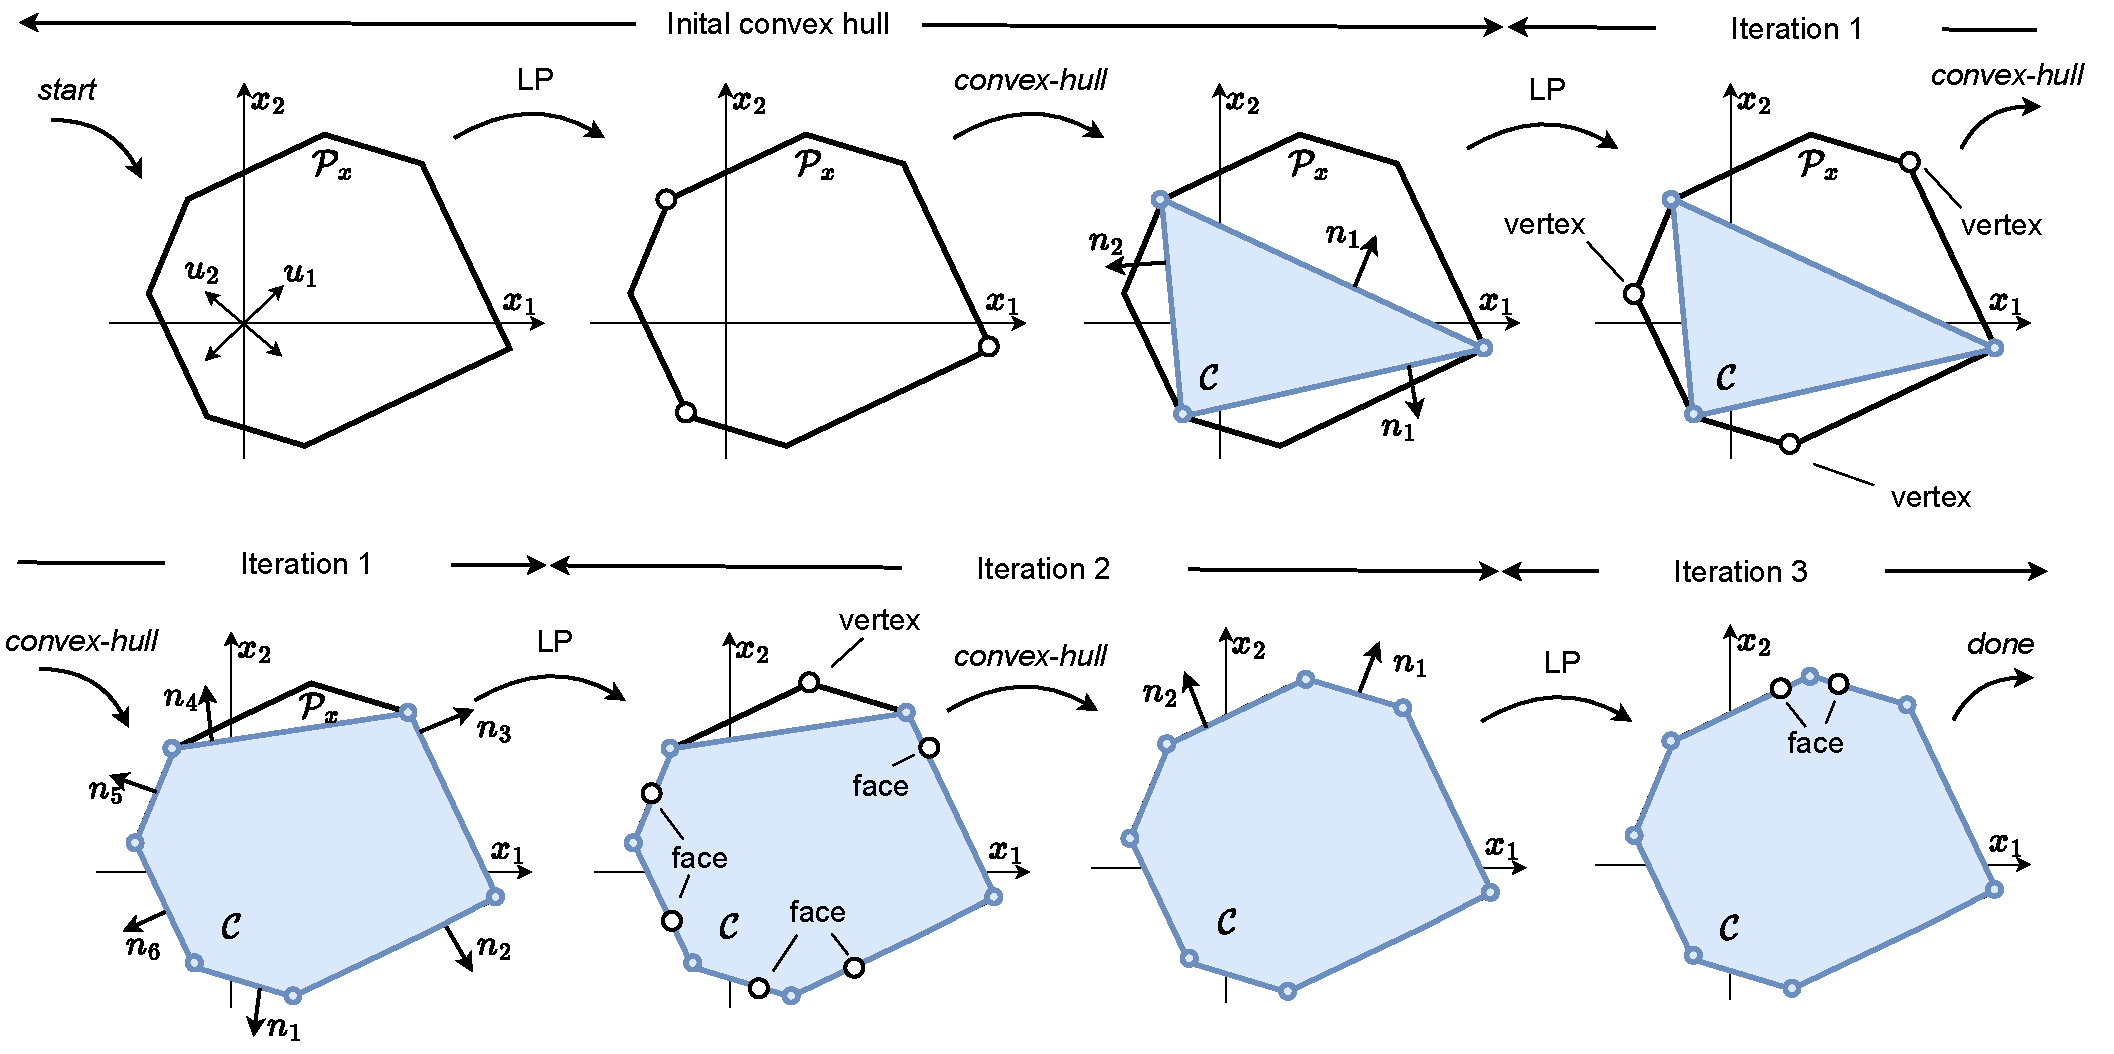
\includegraphics[width=\linewidth]{Papers/images/ichm_full.pdf}
    \vspace{-0.8cm}
    \caption{This figure shows the procedure of the successive approximation of the polytope $\mathcal{P}_x$ using the proposed ICHM algorithm. The approximation starts with the initial Convex-Hull $\mathcal{C}$ construction, using the vectors $\bm{u}_i\in U$. Then the approximation is refined by using the face normal vectors $\bm{n}_i$ of the Convex-Hull $\mathcal{C}$ with the \gls{lp} (\ref{eq:lin_prog}) to find new vertices which are then used to update the Convex-Hull $\mathcal{C}$. The check (\ref{eq:normal_coplanar_test}) is used to determine if the \gls{lp} results belong to the faces or they are new vertices of the polytope. The algorithm stops when no new vertices are found. }
    \label{fig:algo_example}
\end{figure}


\begin{wrapfigure}{r}{0.35\linewidth}
\vspace{-1.5cm}
    \centering
    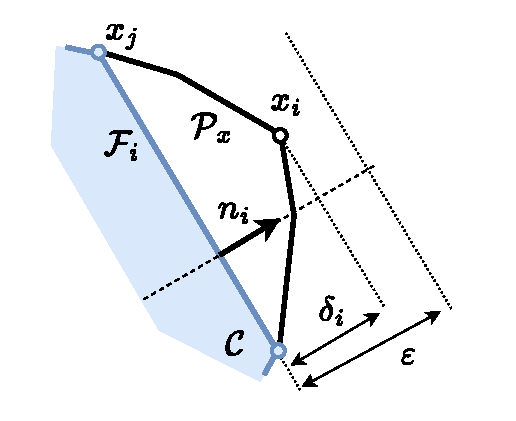
\includegraphics[trim=2.5cm 2cm 0 0,clip=true,width=\linewidth]{Papers/images/espilon_explicaiton.pdf}
    \caption{ The figure shows an example of the polytope face condition from equations (\ref{eq:normal_coplanar_test}) and (\ref{eq:normal_distance}). The face $\mathcal{F}_i$ of the Convex-Hull $\mathcal{C}$ is considered to be the face of $\mathcal{P}_x$, because $\delta_i\! < \!\varepsilon$. }
    \label{fig:expilon_explication}
\end{wrapfigure}
\subsubsection{Incremental refinement} The next step of the algorithm is to iterate over all the faces $\mathcal{F}_i$ of the Convex-Hull $\mathcal{C}$. For each new face $\mathcal{F}_i$, the normal $\bm{n}_i$ is found and used as a candidate $\bm{c}_i$ in the direction pointing out of polytope $\mathcal{P}_x$.
%all the vertices $\bm{x}_{\mathcal{F}j}\! =\! %\bm{x}_v\!\in\!\mathcal{F}_i$. Then the $\bm{c}_i$ is defined %as normal $\bm{n}_i$ in the direction pointing out of the polytope 5$\mathcal{P}_x$.
The normal vector direction is verified by projecting the vector going from the centroid $\bm{x}_c$ to any vertex $\bm{x}_{j}$ of face $\mathcal{F}_i$, onto the normal $\bm{n}_i$ and verifying if the scalar product is positive or negative.\\
\begin{equation}
    \bm{c}_i = \begin{cases}
  \bm{n}_i, & \text{if } \bm{n}_i^T(\bm{x}_{j} - \bm{x}_c) \geq 0, \\
  -\bm{n}_i, & \text{otherwise}.
\end{cases} 
\label{eq:normal_condition}
\end{equation}
Solving equation (\ref{eq:lin_prog}) with $\bm{c}_i$, the obtained $\bm{x}_i$ can be either a vertex of the polytope $\mathcal{P}_x$ or be coplanar with face $\mathcal{F}_i$. To determine if  $\bm{x}_i$ is coplanar with the face, a simple check can be devised, which verifies if the orthogonal (normal) distance from $\bm{x}_i$ to any vertex $\bm{x}_{j}$ of face $\mathcal{F}_i$
\begin{equation}
    \delta_i = \bm{n}_i^T(\bm{x}_{j} - \bm{x}_i)
\label{eq:normal_distance}
\end{equation}
is within a certain user defined accuracy $\varepsilon$
\begin{equation}
    \bm{x}_i = \begin{cases}
   \text{vertex}, & \text{if }  |\delta_i| \geq \varepsilon, \\
    \text{on the face}, & \text{otherwise}.
\end{cases} 
\label{eq:normal_coplanar_test}
\end{equation}
\Cref{fig:expilon_explication} provides a graphical interpretation of this check and of the values $\delta_i$ and $\varepsilon$.

If $\bm{x}_i$ belongs to face $\mathcal{F}_i$ of the Convex-Hull $\mathcal{C}$ then  $\mathcal{F}_i$ is considered to be a face of the polytope $\mathcal{P}_x$. In that case the algorithm updates the $\repr{H}$-representation of $\mathcal{P}_x$ 
\begin{equation}
    H \leftarrow \begin{bmatrix} H \\ \bm{n}_i^T\end{bmatrix}, \quad \bm{d} \leftarrow \begin{bmatrix}  \bm{d} \\ \bm{n}^T_i \bm{x}_{j} \end{bmatrix}
\label{eq:h_rep}
\end{equation}
where $\bm{n}_i$ is the face normal vector and $\bm{n}_i^T \bm{x}_{j}$ is the orthogonal distance from the origin to the face $\mathcal{F}_i$. On the other hand, if $\bm{x}_i$ is a vertex of the polytope it is appended to the $\repr{V}$-representation list $X_v \leftarrow [X_v, ~\bm{x}_i]$.

\subsubsection{Stopping condition} 
Once all the faces of the Convex-Hull $\mathcal{C}$ are evaluated, the Convex-Hull is updated using the new vertex list $X_v$.

One of the algorithm stopping conditions proposed by \citet{Bretl2008}, is to construct the inner and outer approximation of the polytope $\mathcal{P}_x$ at the same time and stop approximating when the ratio $r=\vol{\mathcal{P}_{inner}}/\vol{\mathcal{P}_{outer}}$ between their volumes reaches a certain threshold $r\leq1$.  

However, volume ratio condition is sometimes hard to interpret, as its representation of the approximation error does not have the same units as the physical quantity being represented by the polytope $\mathcal{P}_x$. Therefore, the ICHM algorithm exploits a different stopping condition setting the threshold on the maximal distance $\delta_i$. The algorithm stops iterating if the vertex list $X_v$ has no new elements or, in other words, if the maximal distance $\delta_i$ for all the faces $\mathcal{F}_i$ is lower than the user defined accuracy $\varepsilon$  
\begin{equation}
    \max\{|\delta_{i}|\} \leq \varepsilon
\end{equation}
In this stopping condition, the maximal distance $\delta_i$ corresponds to the maximal error committed by the approximation, expressed with the same units as the units of the physical quantity being represented by the polytope. Provided that the output space has the same units in all the axis. Preserving the same units improves the interpretation of the approximation error and enables the user to intuitively decide on the acceptable approximation error $\varepsilon$ for the application in question. 

Finally, if the user sets the approximation error $\varepsilon\!=\!0$, the ICHM algorithm finds the exact solution, all the vertices and the faces of the polytope $\mathcal{P}_x$.

\subsection{Performance analysis}
\label{ch:chm_performance}

To evaluate the efficiency of the ICHM algorithm, the challenging polytope formulation, corresponding to the generic formulation (\ref{eq:generic_polyt_view_revisit2}), with a high-dimensional input space and a low-dimensional output space ($n\gg m$) is tested. Additionally, the algorithm performance is compared against two state-of-the-art approaches: an approximation approach based on the \gls{rsm} algorithm introduced by \citet{carmichael_towards_2011} and an exact evaluation approach based on the combination of two efficient algorithms \gls{hpsm} \cite{hyper_psm} and \gls{pim} \cite{bremner_fukuda_marzetta_1998}.

\subsubsection{Human wrench capacity polytope}
The polytope in question is the human's wrench capacity polytope, previously discussed in \Cref{ch:force_poly_human}. The polytope $\mathcal{P}_f$ characterising the achievable wrenches $\bm{f}$, the human can generate given its musculoskeletal model, can be expressed as 
\begin{equation}
    \mathcal{P}_f(\bm{q},\dot{\bm{q}},\ddot{\bm{q}}) = \left\{ \bm{f} \in \mathbb{R}^m ~|~ \bm{F}\in\left[\bm{F}_{min}, \bm{F}_{max} \right], ~~ \!J^T(\bm{q})\bm{f} =\! N(\bm{q})\bm{F} -\bm{\tau}_b(\bm{q},\dot{\bm{q}},\ddot{\bm{q}}) \right\}
    \label{eq:human_force_poly_revisit2}
\end{equation}
where $\bm{f}\in\mathbb{R}^m$ is the \gls{cs} wrench, $\bm{F}\in\mathbb{R}^n$ is the vector of muscular forces, while $J(\bm{q})$ and $N(\bm{q})$ are configuration $\bm{q}$ dependant Jacobian and moment arm matrix. Additionally, the bias vector $\bm{\tau}_b$ corresponds to the joint torques corresponding to the effects of the gravity and the movement. 

% \begin{landscape}
\begin{figure}[!t]
    \centering
    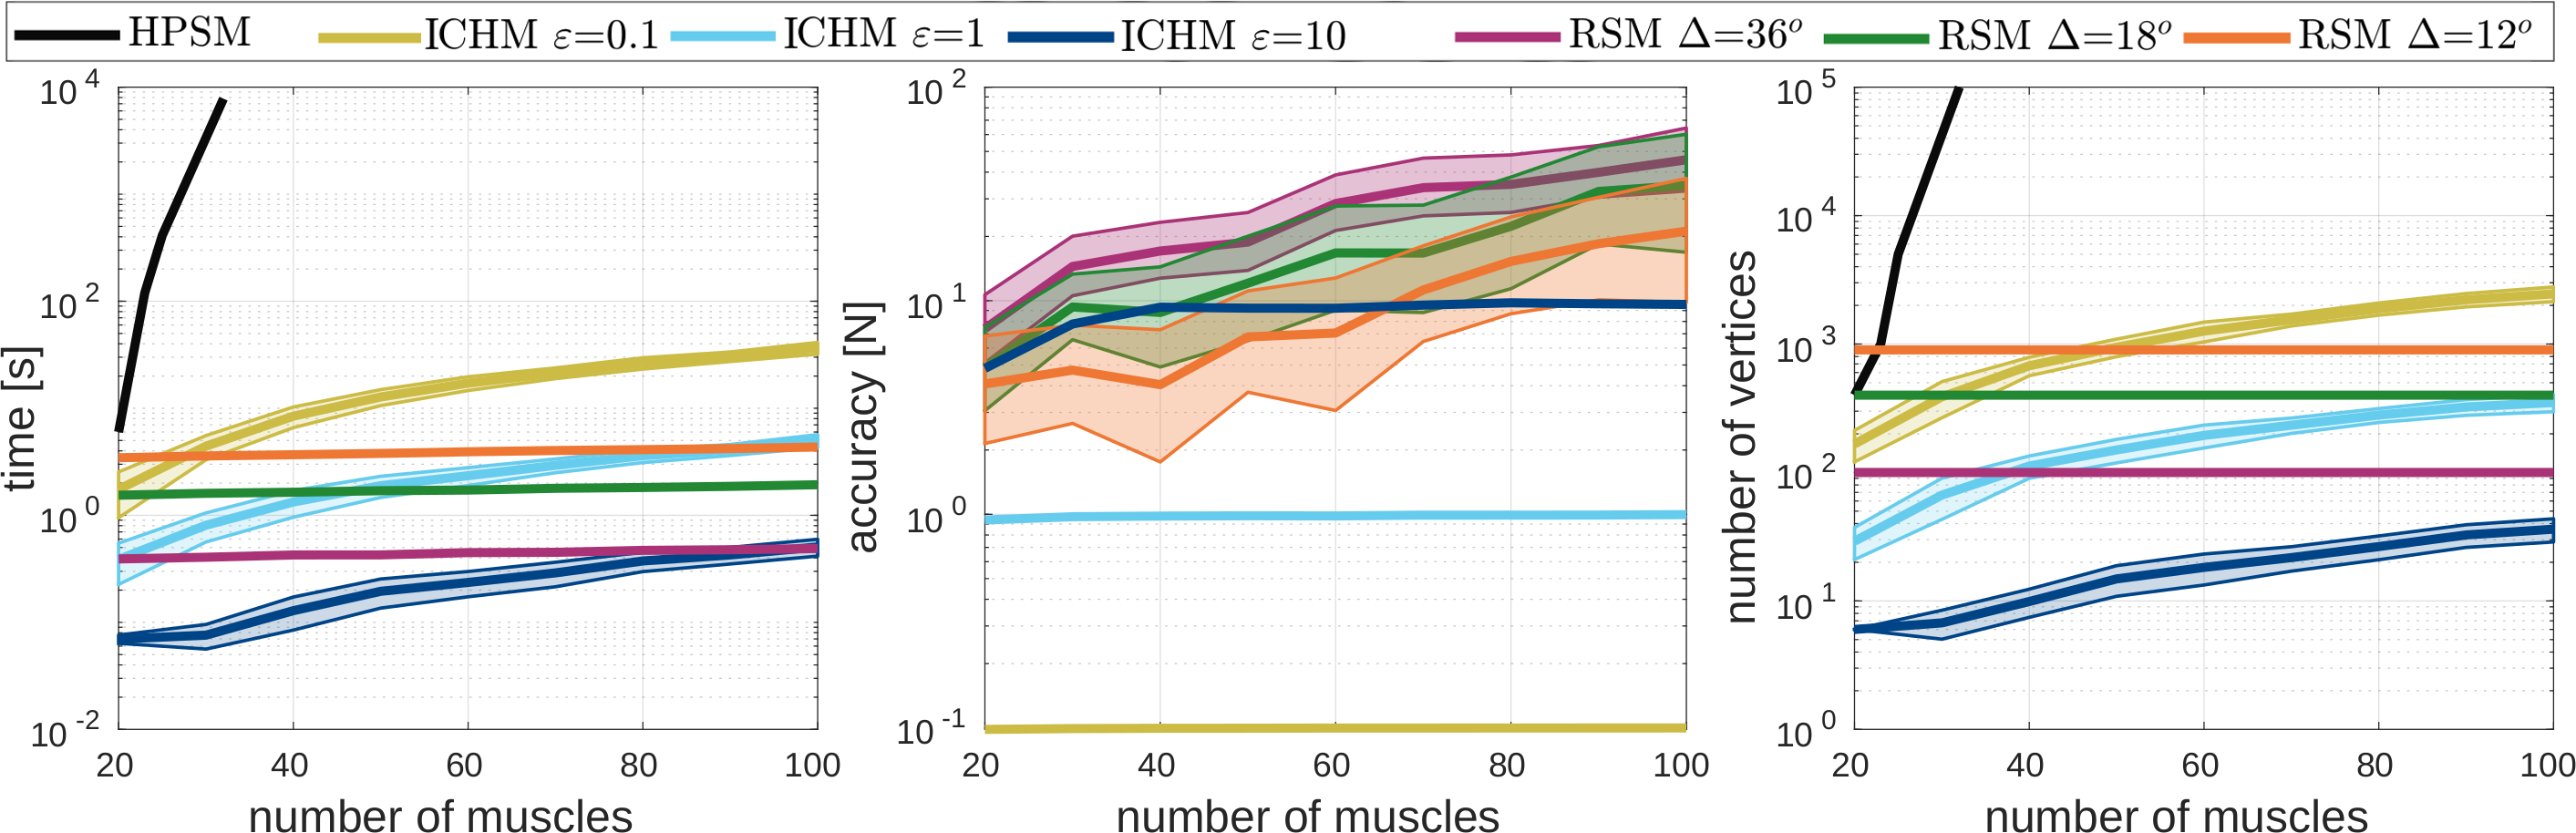
\includegraphics[width=\linewidth]{Papers/images/one_auto_new5_these.png}
    \caption{{Figure presenting the performance analysis results in the logarithmic scale for three different algorithms: \gls{hpsm}, \gls{rsm} and proposed ICHM with respect to different number of muscles. The left figure shows the evolution of the execution time. The middle figure shows the evolution of the underestimation error, the maximal distance in between the polytope $\mathcal{P}_x$ and the acquired polytope, calculated as max$\{|\delta_{i}|\}$. The right figure shows the evolution of the number of vertices found. All the plots show the averaged results, with variances, over 100 runs, where each run corresponds to one randomly generated model.}}
    \label{fig:performance_results}
\end{figure}
% \end{landscape}
This polytope formulation is challenging due to the high dimensional input space (large number of muscles), making the geometry of the polytope $\mathcal{P}_f$ relatively complex, having large number of faces and vertices. In such cases, standard exact methods for polytope transformation have long execution times, preventing this polytope representation to be used in interactive (online) applications. To reduce the computation times of the wrench polytope $\mathcal{P}_f$ evaluation, \citet{carmichael_towards_2011} have proposed an algorithm based on the \gls{rsm}, described in \Cref{ch:approximation_algos}. Although the algorithm enables real-time approximation of the polytope $\mathcal{P}_f$, the obtained approximation is coarse and without any bounds on the approximation accuracy. 


\subsubsection{Experiment and results}
Therefore, to evaluate the performance of the proposed ICHM algorithm, a comparative experiment is
performed, where the ICHM algorithm's performance is compared against the \gls{rsm} method proposed by \citet{carmichael_towards_2011} as well as against the two step exact approach based on the \gls{hpsm} \cite{hyper_psm} and \gls{pim} \cite{bremner_fukuda_marzetta_1998}. The experiment consists in finding the $\repr{V}$-representation of the \gls{cs} force $m=3$ polytope $\mathcal{P}_f$ for a randomised mock-up musculoskeletal model with $k\!=\!7$ degrees of freedom and a number of muscles ranging from $n$ = $20$ to $100$. 

The \gls{rsm} algorithm \cite{carmichael2011Towards} requires uniform sampling of the ray directions in the 3D space. In this experiment the sampling is performed based on a two Euler angles parametrisation. {For this method, three linearly increasing levels of granularity are tested for each Euler angle: $\Delta\!=\!36^o$, $18^o$ and $12^o$;  making for $n_r\!=\!10,20$ and $30$ rays per angle. Overall number of ray directions in 3D space ($N_r\!=\!n_r^2$) is then $100$, $400$ and $900$. For the proposed ICHM algorithm, three exponentially increasing levels of accuracy are tested $\varepsilon\!=\!0.1$, $1$ and $10$ N.} All the algorithms are implemented in Matlab and run on a 1.90GHz Intel i7-8650U processor. The source code of the experiment is publicly available on GitLab\footnote{Gitlab: \url{https://gitlab.inria.fr/auctus-team/people/antunskuric/papers/human_wrench_capacity}}.

Results of the experiments, averaged over 100 algorithm runs, are shown on \Cref{fig:performance_results}. The results confirm that the exact approach using the \gls{hpsm} method has an execution time exponentially related to the number of muscles. Even for only 30 muscles it already takes more than 4.5 h to calculate, therefore this method is not tested on more than 30 muscles, where it finds over $10^4$ vertices.  

\begin{figure}[!t]
    \centering
    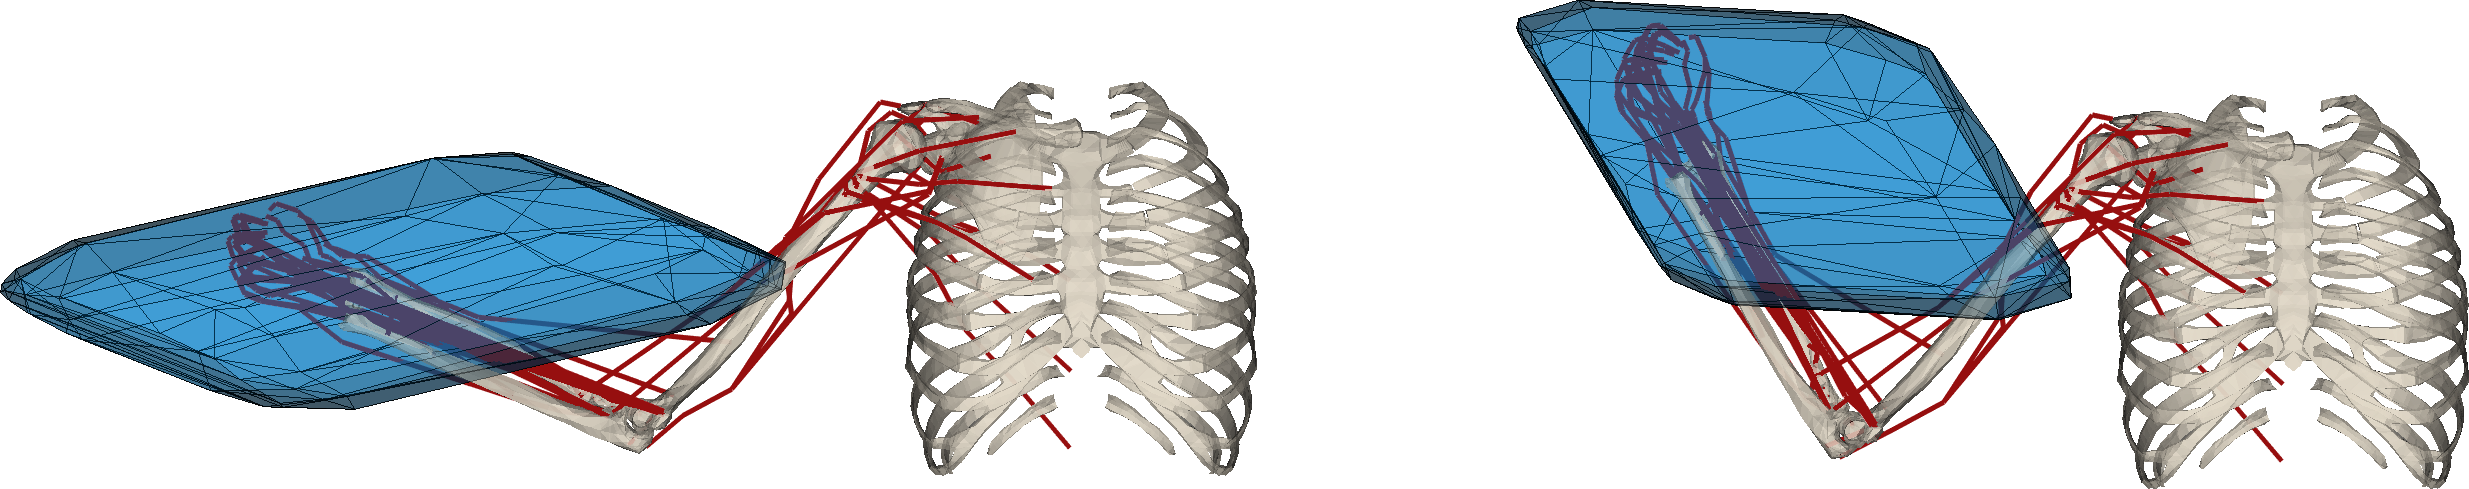
\includegraphics[width=\linewidth]{Papers/images/force.png}
    \caption{\gls{cs} force polytope of a musculoskeletal model of human upper limb  \cite{saul2015benchmarking} with 7DOF and 50 muscles, evaluated for two different configurations using the proposed ICHM algorithm. The visualisation is performed using \codet{bioviz} \cite{Michaud2021} and polytopes are scaled with a ratio 1m : 1000N}
    \label{fig:images_bimanual}
\end{figure}
The \gls{rsm} algorithm shows nearly constant time of execution for the full range of tested muscles and the constant number of vertices found, which is expected. The results show however, that for low muscle numbers $d\!<$25, when using a fine granularity $\Delta$=$12^o$ the \gls{rsm} algorithm finds more vertices than the exact solution found by the \gls{hpsm}. Furthermore, the middle plot of \Cref{fig:performance_results} shows that the \gls{rsm} estimation error increases considerably with the number of muscles $d$, followed by a very
high variance. These results confirm that, as the polytope shape is not spherical, by uniformly covering the space of ray directions, \gls{rsm} based algorithms will necessarily estimate certain areas of the polytope better than the others.

The graphs show that the proposed ICHM method's execution time depends near-linearly of the number of muscles considered $d$ and the estimation error bound parameter $\varepsilon$. The accuracy graph, shown in the middle plot, shows that the proposed ICHM algorithm is capable of limiting the estimation error of the polytope evaluation under desired value $\varepsilon$ regardless of the number of muscles. Furthermore, considering the vertex number found by the algorithms, it can be seen that the number of vertices has a nearly-linear relationship with the number of muscles $d$ and the variable $\varepsilon$. 

The demonstrated efficiency of the ICHM algorithm opens many doors for its applications in real-time systems, providing the user with an easy to understand trade-off between speed and accuracy. 
\Cref{fig:images_bimanual} shows the visualisation of the \gls{cs} force ($m=3$) polytope of a human musculoskeletal model with 50 muscles and 7DOFs, calculated using the ICHM algorithm.


\newpage
\subsection{Algorithm implementation}
\qrimg{qrcodes/pycapacity.png}{https://auctus-team.github.io/pycapacity/}{\codet{pycapacity}}
The pseudo-code of the ICHM algorithm is given in \Cref{alg:algo_2}, while an efficient open-source Python implementation is publicly available within the package \codet{pycapacity}\footnote{\href{https://auctus-team.github.io/pycapacity/}{https://auctus-team.github.io/pycapacity/}}, which is described more in detail in \Cref{ch:software}.

Finally, \Cref{ch:human_robot_carrying} brings the application of the proposed algorithm for the real-time robot control in the human-robot collaboration scenario, where the algorithm is exploited in order to calculate the human's wrench capacity polytope online. 


\begin{algorithm}[!h]
\caption{Proposed ICHM algorithm pseudo-code}
\begin{algorithmic}
\REQUIRE $A$,$B$, $\bm{y}_{min}$, $\bm{y}_{max}$, $\bm{b}$, $\varepsilon$
\STATE $U, \Sigma, V^T \leftarrow svd(A^+)$ 

\STATE init $\repr{H}$-rep: $H,\bm{d} \leftarrow [\,]$ and $\repr{V}$-rep: $\bm{x}_v,\bm{y}_v\leftarrow [\,]$
\STATE \textbf{for all}   {$\bm{u}_i$ in $U$} \textbf{do}

\hspace{0.3cm} $\bm{y}_{i}\leftarrow$ \gls{lp} (Eq. \ref{eq:lin_prog}) with $\bm{c}\! =\! \bm{u}_i$ and $\bm{c}\! =\! -\bm{u}_i$

\hspace{0.3cm} $\bm{x}_{v} \leftarrow [\bm{x}_{v}, ~ A^+B\bm{y}_i + A^+\bm{b}]$

\REPEAT

\STATE calculate the Convex-Hull $\mathcal{C}$ of $\bm{x}_{v}$
\STATE calculate the centroid $\bm{x}_{c} = \frac{1}{N}\sum_i\bm{x}_{v,i}$

\STATE \textbf{for all}   {new face $\mathcal{F}_i$ in $\mathcal{C}$} \textbf{do}
%\FORALL{ new face $\mathcal{F}_i$ in $\mathcal{C}$ } 

\hspace{0.25cm} find normal $\bm{n}_i$ and one vertex $\bm{x}_{j}$ of $\mathcal{F}_i$

\hspace{0.25cm} $\bm{y}_{i}\leftarrow$ \gls{lp} ( Eq. \ref{eq:lin_prog} ) with  $\bm{c}\! =\! \bm{n}_i$ ( Eq. \ref{eq:normal_condition} )

\hspace{0.25cm} $\bm{x}_{i} = A^+B\bm{y}_i+A^+\bm{b}$ 

\hspace{0.25cm}  calculate $\delta_i$ (Eq.\ref{eq:normal_distance})

\hspace{0.25cm}  \textbf{if}   $ |\delta_i| \leq \varepsilon$ \textbf{then} 

\hspace{0.6cm}  new face: update $\repr{H}$-rep  ( Eq. \ref{eq:h_rep} )

\hspace{0.25cm}  \textbf{else}

\hspace{0.6cm} new vertex: update $\repr{V}$-rep: $\bm{x}_{v} \!\leftarrow\! [\bm{x}_{v},~ \bm{x}_i ]$,  $\bm{y}_{v} \!\leftarrow\! [\bm{y}_{v},~ \bm{y}_i ]$ 

%\ENDFOR
\UNTIL{{ $\max\{|\delta_{i}|\}\leq \varepsilon$}}
\RETURN  $\repr{V}$-rep: $\bm{x}_v$, $\bm{y}_v$ and  $\repr{H}$-rep: $H$, $\bm{d}$ 
\end{algorithmic}
\label{alg:algo_2}
\end{algorithm}

\section{Conclusion}

This chapter aims to provide a set of tools for efficient transforming of polytopes representing the physical abilities of humans and robots into more standardised forms suitable for practical applications. The focus is put on the two widely used polytope representations: vertex or $\repr{V}$ and half-plane or $\repr{H}$-representations. These representations offer various advantages, including compatibility with visualisation tools, in a for triangulated meshes, and optimisation-based applications like robot control and trajectory planning. Additionally, they enable efficient operations like Minkowski sums and intersections over multiple polytopes.

While the literature presents numerous algorithms for transforming polytope formulations into their $\repr{H}$ or $\repr{V}$-representation, these algorithms are often tailored to specific sets of polytope formulations. \Cref{ch:phisical_ability_metrics} proposes a generic view on different common polytope representation of humans' and robots' physical abilities and proposed a unifying polytope formulation describing all the proposed metrics, introduced in \Cref{ch:collab_metrics_overview}. However, this unified formulation is not directly suitable for the standard polytope transformation algorithms. Hence, \Cref{ch:generic_view} proposes a structured view on different polytope formulation families derived from the proposed generic unified formulation namely intersection and projection formulation, as well as some special cases.

\Cref{ch:polytope_algorithms} further provides an overview of applicable techniques for transforming these families into their $\repr{V}$ or $\repr{H}$-representation. The chapter briefly introduces the standard generic methods for mutual transformation between $\repr{V}$ and $\repr{H}$-representation, followed by the polytope formulation specific methods that are capable of better exploiting the geometry of the formulation families. Finally, several polytope approximation methods are discussed as a means of improving the efficiency of polytope transformation for high-dimensional problems. 
The aim of this overview is to provide a brief introduction into the applicable state-of-the-art methods when it comes to transforming different polytope formulations as well as to discuss their limitations and computational efficiency.

The final two sections of this chapter introduce two contributions of this thesis in the domain of polytope transformations. The \Cref{sec:algorithm_vea} introduces an efficient vertex enumeration algorithm for the intersection polytope formulation with the interval input set. This algorithm is based on the work by \citet{sasaki2011vertex}, exploiting the geometry of the hyperrectangle input set in order to improve its computational complexity of its exhaustive search and reduce the execution time. The algorithm is particularly well suited for low dimensional polytope evaluation, that are common when it comes to polytope characterisations of physical abilities of robotic manipulators. The performance of the proposed algorithm is compared to the state-of-the-art methods on finding the $\repr{V}$-representation of the force capacity polytope for redundant robotic manipulators, introduced in \Cref{ch:poly_force}. The results show that the algorithm has significantly lower computational complexity and hence shorter execution time, in the order of magnitude of several milliseconds for standard robotic manipulators, implemented in Pyhton. Such short execution time opens doors for using these polytopes in real time applications, such as robot control. This algorithm has been published in the context of the scientific paper \citet{skuric2021robot}.

\Cref{ch:algorihtm_ichm} brings a new polytope approximation algorithm based on the \gls{chm} by \citet{lassez1992quantifier}. The algorithm is developed for the generic polytope formulation directly and can therefore be used with all the common polytope formulation introduced in previous chapter. This algorithm performs an iterative approximation of the final polytope by using sequences of \glspl{lp} to find new vertices of the polytope and Convex-Hull to group the to faces. The algorithm improves the approximation accuracy in each iteration and continues iterating when desired user defined approximation accuracy is reached. The execution time of the algorithm depends directly of the complexity of the polytope being transformed (number of faces and verteices), therefore by appropriately setting the desired accuracy, the algorithm is capable of simplifying the final geometry of the polytope and lowering the execution time. This is particularly useful when it comes to the high-dimensional problems, where the input space dimension is much higher than the output space $n\!\gg \!m$, where the standard exact methods have intractable execution times, as they are based on different forms of the exhaustive search. Such high-dimensional problems are very common when it comes to characterising physical abilities of humans based on their musculoskeletal models, as they often have large number of muscles $n$, while their capacities are characterised in the \gls{cs} $m=3$. The performance of the proposed method is therefore tested on the challenging polytope formulation of the human's wrench capacity polytope, described in \Cref{ch:force_poly_human}. The results of the proposed methods in comparison to the state-of-the-art methods show that it has significantly shorter computation time while at the same time guaranteeing the user defined approximation accuracy. Furthermore, the results show that the proposed algorithm, in the case of human's wrench capacity polytope, has execution time under half of a seconds for musculoskeletal models up to 100 muscles, opening many doors for using this polytope formulation in the real time applications. The ICHM algorithm has been published in the context of the scientific paper \citet{Skuric2022human} and later refined within \citet{skuric2023dynamics}.

Following chapter leverages the proposed algorithms and formulations to propose several use-cases of the polytope based physical ability characterisations in the context of the real-time robot control in different human robot physical collaboration scenarios. 
\Cref{ch:physical_interaction} proposes uses the real-time polytope evaluation for creating more adapted robot control strategies in the context of the physical human-robot interaction. 
\Cref{ch:informaiton_polytopes} explores the possibilities of using polytopes for the real-time visual feedback to the operators. Moreover, \Cref{ch:topca} proposes a new \gls{cs} trajectory planning strategy exploiting the polytope algebra. Finally, \Cref{ch:software} presents the publicly available open-source software package implementing several algorithms introduced in this section and enabling an efficient, real-time compatible, evaluation of polytope based physical abilities for humans and robots.


% \part{Theoretic contribution}
% 

\newcommand{\onum}[1]{\overline{{#1}}} 	%upper limit interval
\newcommand{\unum}[1]{\underline{{#1}}}  	%lower limit interval

\chapter{Force capacity polytope algorithm for robots}
% \todo[inline]{David et Vincent: Je vous propose à utiliser les commentaires "tab review" pour gérer les changements un peu plus simplement}
%%%%%%%%%%%%%%%%%%%%%%%%%%%%%%%%%%%%%%%%%%%%%%%%%%%%%%%%%%%%%%%%%%%%%%%%%%%%%%%%

Ellipsoid-based manipulability measures are often used to characterize the force/velocity task-space capabilities of robots. While computationally simple, this approach largely approximates and underestimates the true capabilities. Force/velocity polytopes appear to be a more appropriate representation to characterize the robot's task-space capabilities. However, due to the computational complexity of the associated vertex search problem, the polytope approach is mostly restricted to  offline use, \textit{e.g.} as a tool aiding robot mechanical design, robot placement in work-space and offline trajectory planning. In this paper, a novel on-line polytope vertex search algorithm is proposed. It exploits the parallelotope geometry of actuator constraints. The proposed algorithm significantly reduces the complexity and computation time of the vertex search problem in comparison to commonly used algorithms. In order to highlight the on-line capability of the proposed algorithm and its potential for robot control, a challenging experiment with two collaborating \textit{Franka Emika Panda} robots, carrying a load of 12 kilograms, is proposed. In this experiment, the load distribution is adapted on-line, as a function of the configuration dependant task-space force capability of each robot, in order to avoid, as much as possible, the saturation of their capacity.
% The algorithm execution time for 7DOF \textit{Franka Amika Panda} and for 6DOF \textit{Universal Robots UR5} robots is under 3 and 2 milliseconds respectively.


%%%%%%%%%%%%%%%%%%%%%%%%%%%%%%%%%%%%%%%%%%%%%%%%%%%%%%%%%%%%%%%%%%%%%%%%%%%%%%%%
\section{Introduction}

\begin{figure}[!h]
    \centering
        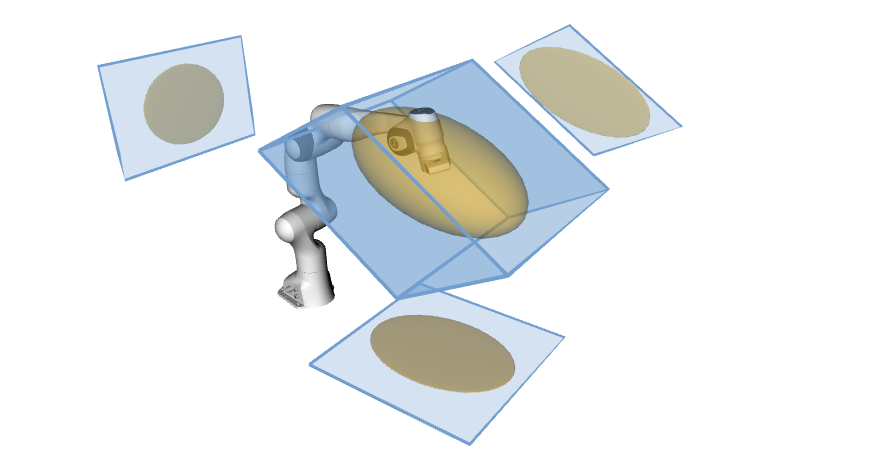
\includegraphics[width=0.8\linewidth]{Papers/images/polytope_ellipsoid.png}
    \caption{2D and 3D force polytopes and their ellipsoid counterparts for a 7 degrees of freedom (DoF) \textit{Franka Emika Panda} robot. Both polytopes and ellipsoids are calculated separately for the 3D and for each of the 2D reduced task-space cases. Both polytopes and ellipsoids take in consideration the true joint torque limits provided by the manufacturer. The underestimation of the true force capabilities of the robot by ellipsoids appears clearly.}

    \label{fig:polytope_ellipsoid}
    \vspace*{-0.3cm}
\end{figure}

Robotics manipulators and their environments are traditionally optimised for a set of specific tasks and their efficiency is based on long-term task execution. Recently, with the introduction of collaborative robots in human environments, robots need to be adaptable to unexpected events, flexible in both task definition and execution and provide high degree of safety for all humans involved. Therefore, evaluating robot capabilities and optimising their performance in advance, with tools designed for more traditional robots, is no longer a suitable approach. New on-line capable and accurate evaluation techniques are needed to account for constantly changing environments, flexible tasks and interaction requirements of collaborative robots.

There are several types of metrics developed to characterise robot's kinematic, kineto-static and dynamic capabilities. The characteristics of robots are related to their kinematics, mechanical design and actuation/joint limits. Kineto-static capabilities of robots characterize the ranges of achievable twists and wrenches in arbitrary directions while in \textit{static conservative conditions}\cite{angeles_design_2016}. Dynamic capabilities characterise ranges of achievable accelerations and link elastic deformations. 

Arguably the most widely used metrics are kineto-static capacity metrics based on \textit{dexterity indices}, expressing robot's ability to move and apply forces and torques in arbitrary directions with equal ease \cite{angeles_design_2016}. The widely used implementation of this metric are velocity and force manipulability ellipsoids, introduced by Yoshikawa \cite{yoshikawa_manipulability_1985}. 
On the one hand, velocity manipulability ellipsoids are often used as a performance measure to optimise robot trajectories and avoid unwanted configurations. On the other hand, force manipulability ellipsoid characterises the forces the robot can apply or resist based on its kinematics. It is used during the design stage of robotic manipulators \cite{angeles_design_2016} as well as for off-line trajectory planning \cite{kuffner_motion_2016} or for on-line control adaptation \cite{joseph2019online}.

Even though manipulability ellipsoids are widely used (mostly because of their calculation efficiency), they are just an approximation and can lead to a drastic underestimation of the real kineto-static capacities of robots \cite{merlet_jacobian_2006}. In the context of collaborative robotics, the margin between the actuation capabilities of the robot and the requirement of the task is largely reduced with respect to more classical, oversized, industrial robots. Thus, any over/under-estimation of the true capabilities of the system has strong negative implications either in terms or safety or in terms of efficiency.

Chiacchio et al.\cite{chiacchio_evaluation_1996} demonstrated that the exact wrench and twist capacities have the form of polytopes. Polytopes do not underestimate the robot capacity \cite{finotello_computation_1998}, can easily integrate variable and non-symmetric limits, dynamics and external forces \cite{merlet_jacobian_2006}. Additionally, in the context of collaborative robotics, when evaluating capacities of multiple robots, sum and intersection of ellipsoids becomes a complex problem to solve and interpret \cite{lee_dual_1989}\cite{chiacchio_task_1991}\cite{julio_frantz_analysis_2015} whereas these operations are well-defined for polytopes. Figure~\ref{fig:polytope_ellipsoid} illustrates the difference of force capability estimation between polytope and ellipsoid characterization.
%Furthermore, since the ellipsoids are considerable underestimation of robot capacities it is certainly important to question the energy efficiency and safety implications.
However, evaluating twist and wrench polytopes relies on a \textit{vertex enumeration} problem \cite{avis_pivoting_nodate} which is a computationally intensive task and is the main obstacle for wider uses of polytopes instead of ellipsoids in practice. 

In this paper, a brief overview of polytope-based task-space capability characterization is given in section~\ref{sec:section_rappel}. Then, a new on-line capable polytope vertex finding algorithm for efficiently calculating twist and wrench polytopes is proposed and described in section~\ref{sec:algorithm}. The new algorithm is capable of calculating polytope vertices for 6DoF and 7DoF robots under 3ms in Python as illustrated in section~\ref{sec:results}. This opens many doors in terms of on-line usage of such capability indicators. To demonstrate the benefits of our method for on-line robot control, an experimental setup with two collaborating \textit{Franka Emika Panda} robots is proposed. It is shown that by leveraging the real carrying capacity on-line measure of the robots, it is possible to design a control strategy allowing to carry, a voluntarily exaggerated, mass of 12 kilograms.  Discussions on the potential applications of the results of this work in collaborative robotics are then proposed in section~\ref{sec:discussion}.


\section{Task-space twist and wrench feasibility polytopes basics}
\label{sec:section_rappel}
For a serial robotic manipulator with $n$ degrees of freedom, with joint space generalized coordinates $\bm{q} \in \mathbb{R}^{n}$ and with Jacobian matrix $J(\bm{q})\in \mathbb{R}^{m \times n}$ (with $m=6$ in the 3D case and $m=3$ in the planar one), the task space Cartesian twist  $\bm{v}$ can be calculated from generalized velocities $\bm{\dot{q}}$ using
\begin{equation}
    \bm{v} = J(\bm{q})\bm{\dot{q}}
    \label{eq:velocity}
\end{equation}
The dual relation relaying the Cartesian wrench $\bm{f} \in \mathbb{R}^m$ with the generalized forces $\bm{\tau} \in \mathbb{R}^n$ is given by
\begin{equation}
    J(\bm{q})^T \bm{f} + \bm{\tau}_0 = \bm{\tau}
    \label{eq:force}
\end{equation}
$\bm{\tau}_0$ is a generalized force that does not ``produce'' any task space wrench, \texit{i.e.} $\bm{\tau}_0$ belongs\footnote{We recall here that $\mathcal{K}er(J(\bm{q})) = \mathcal{I}m(J(\bm{q})^T)^\bot$.} to the kernel $\mathcal{K}er(J(\bm{q}))$ of $J(\bm{q})$. Conversely, $(\bm{\tau}-\bm{\tau}_0)$ lies in the image  $\mathcal{I}m(J(\bm{q})^T)$ of  $J(\bm{q})^T$, \textit{i.e.} ``produces'' task space wrenches.

While equations (\ref{eq:velocity}) and (\ref{eq:force}) describe the kineto-static behaviour of a robot, generalized forces $\bm{\tau}$ and velocities $\bm{\dot{q}}$ are constrained due to the physical limits of the robot construction and actuators
\begin{subequations}
\begin{align}
    \unum{\dot{q}}_{i} \leq & \dot{q}_i \leq \onum{\dot{q}}_{i} \label{eq:constraints_v}\\
    \unum{\tau}_{i} \leq &\tau_i \leq \onum{\tau}_{i}  \label{eq:constraints_f}
\end{align}   
\label{eq:constraints}
\end{subequations}
Given these constraints, the feasible twist polytope defined by equation (\ref{eq:velocity}) can be written
\begin{equation}
\begin{split}
    \mathcal{P}_v = & \left\{ \bm{v} \in \mathbb{R}^{m} \,\big| \, \bm{\dot{q}} \in [ \bm{\unum{\dot{q}}}, \bm{\onum{\dot{q}}} ],~\bm{v} = J(\bm{q})\bm{\dot{q}} \right\}
    \label{eq:polytope_v}
\end{split}
\end{equation}

Similarly, the feasible wrench polytope is defined as\footnote{The dependence of $J$ to $\bm{q}$ is dropped here and when further needed for the sake of clarity.}
% \begin{equation}
%   \mathcal{P}_f = \big\{ \bm{f} \in \mathbb{R}^{m} \,| \, \bm{\tau}_{min} \leq \bm{\tau} \leq \bm{\tau}_{max},\quad \bm{f} = J(\bm{q})^{-T} \bm{\tau} \big\}
%  \label{eq:polytope}
% \end{equation}
% where $J(\bm{q})^{-T}$ inverse of the the transposed jacobian matrix. Above  force polytope $\mathcal{P}_f$ formulation is valid only for non-redundant manipulators, where jacobian matrix in invertable. For redundant manipulators a right \textit{pseudo-inverse} $J(\bm{q})^{T+}$  \cite{klema_singular_1980} of matrix $J(\bm{q})^T$ needs to be calculated and the joint torque vector $\tau$ needs to belong to the image of $J(\bm{q})^T$ matrix \cite{chiacchio_evaluation_1996}.

\begin{equation}
\begin{split}
   \mathcal{P}_f = & \left\{ \bm{f} \in \mathbb{R}^{m}\,\big| \bm{\tau} \in \left\{[\bm{\unum{\tau}},\bm{\onum{\tau}}] \cap \mathcal{I}m(J^T)\right\},J^{T}\bm{f}=\bm{\tau} \right\}
 \label{eq:polytope_f}
\end{split}
\end{equation}


%\todo[inline]{not sure should I explain that we cannot put anything in $\tau$ vector and project it to $f$}

\begin{figure}[!t]
    \centering
    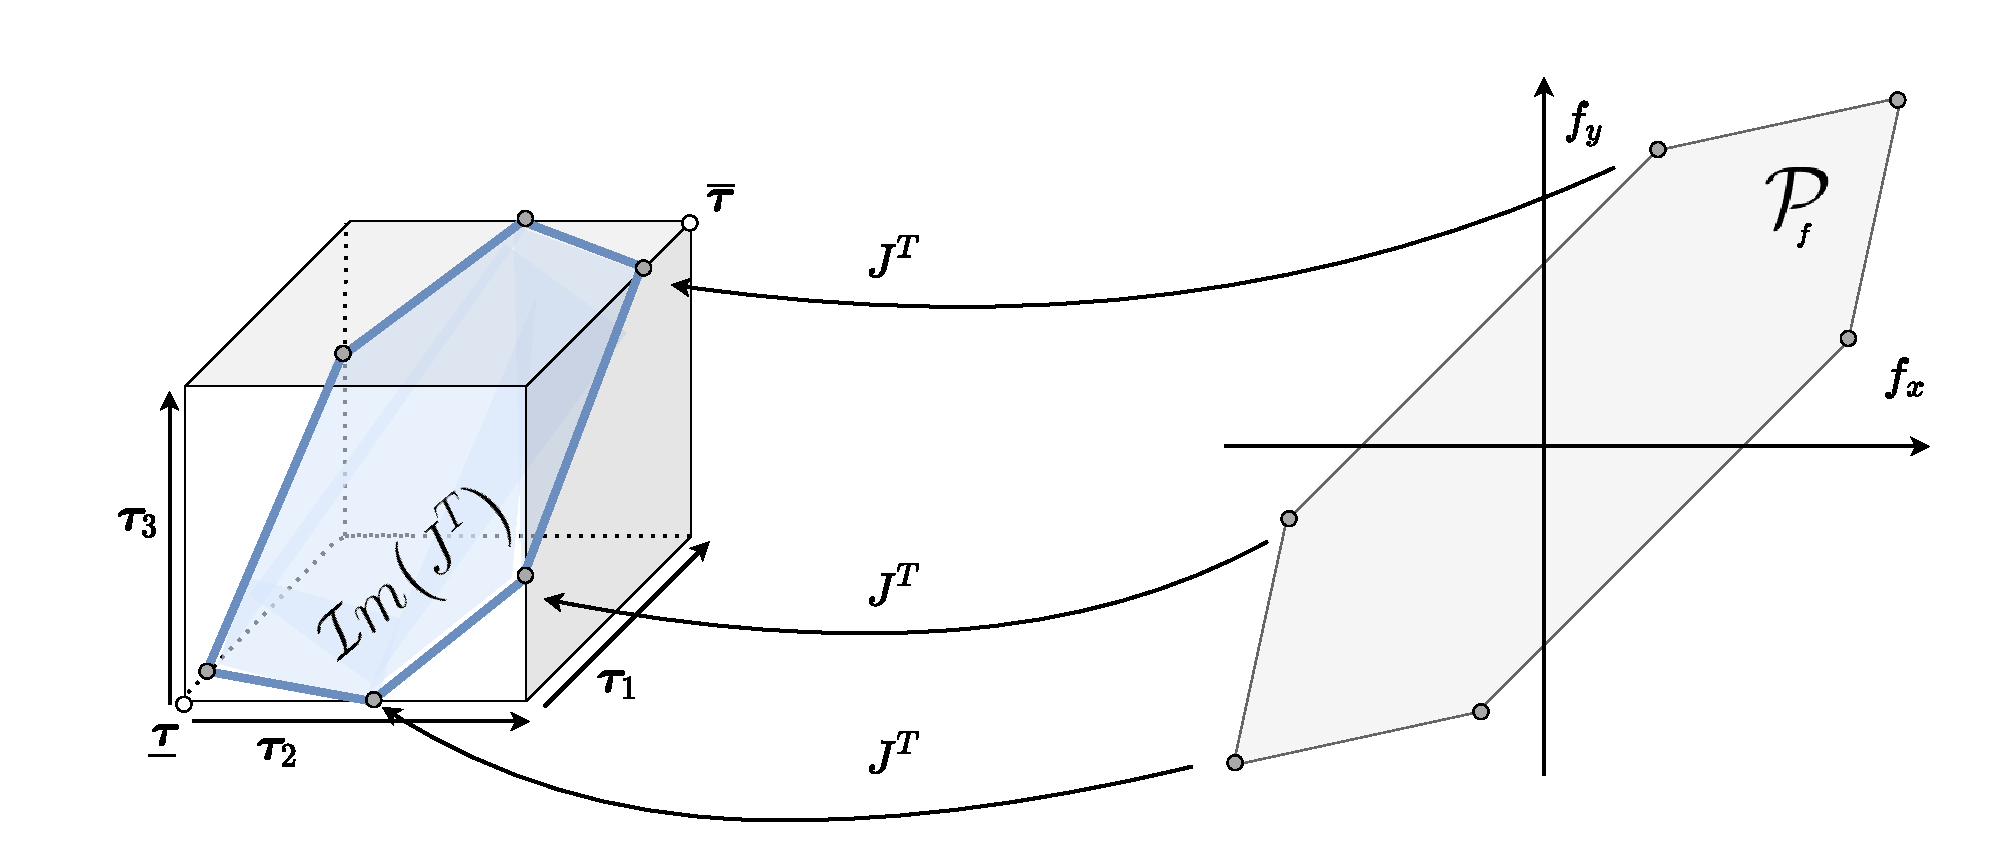
\includegraphics[width=\linewidth]{Papers/images/polytope_search.pdf}
    \caption{Example representation of force polytope $\mathcal{P}_f$ vertices in joint and task-space for a redundant 3DoF planar robot: $n$=$3$, $m$=$2$. }
    \label{fig:polytope_search}
\end{figure}

Equations (\ref{eq:polytope_v}) and (\ref{eq:polytope_f}) provide compact yet implicit representations of the feasible twist and wrench polytope of a robot. The characterization of these capabilities require an explicit definition of these polytopes, \textit{i.e.} a computation of their vertices. In the case of $\mathcal{P}_v$, computing the vertices boils down to determining the convex-hull of the image of the vertices of the constraints polytope defined by equation~(\ref{eq:constraints_v}) through the linear mapping $J(\bm{q})$. The case of $\mathcal{P}_f$ yields an extra difficulty as one first needs to determine the intersection between the constraints polytope defined by equation~(\ref{eq:constraints_f}) and $\mathcal{I}m(J(\bm{q})^T)$.

Over the years many vertex search (enumeration) methods have been proposed \cite{avis_comparative_2015}. Most of the approaches in literature are optimised to solve high dimensional problems and provide an abstraction from the actual system that is being analysed. One of the most commonly used method for vertex enumeration is the double description method \cite{avis_pivoting_nodate} which formulates the vertex search problem as transformation of a half-space representation $\mathcal{H}-rep$ to a vertex representation $\mathcal{V}-rep$. This formulation generalizes well in between different high dimensional problems but lacks the flexibility to incorporate information about the physical system being analysed. 

Therefore, various methods have been introduced in order to leverage specific problem formulation and improve the computational performance of vertex search. The scaling factor method has been developed for planar parallel robots \cite{nokleby_force_2005} and later adapted to planar serial manipulators \cite{julio_frantz_analysis_2015}. This method reduces the search space with one scaling factor to an exhaustive search in the scalar space. A very efficient algorithm for planar robots has also been proposed by Gouttefarde et al. \cite{gouttefarde_versatile_2015} which navigates the polytope boundaries in search for extremities. Both the scaling factor and boundaries navigation methods are designed for planar vertex search and do not scale to three dimensional world.

Chiacchio et al. in their original paper \cite{chiacchio_evaluation_1996} propose an algorithm for finding the vertices of task-space polytopes by introducing slack variables and performing an exhaustive search through the joint space limits. This algorithm, although significantly improving the evaluation still remains too complex for on-line execution. This algorithm has been improved by Sasaki et al. \cite{sasaki_vertex_nodate} where the computational complexity has been significantly reduced by introducing the geometrical representation of actuator constraints as an $n$-dimensional parallelotope.

The next section introduces additional improvements of the algorithms proposed in \cite{chiacchio_evaluation_1996} and \cite{sasaki_vertex_nodate}. The resulting algorithm significantly reduces the computation time and complexity of the vertex enumeration problem for task-space polytopes. The proposed description is restricted to the most complex case of $\mathcal{P}_f$ but the method is also computationally beneficial in the simpler case of computing $\mathcal{P}_v$. Also in order to ease illustrations, the considered task-space wrench is limited to its force component without any loss of generality.

\section{Vertex finding algorithm formulation}
\label{sec:algorithm}
%\todo[inline]{
% \begin{itemize}
%     \item introduce the new algorithm
%     \item pseudocode maybe
%     \item nice figure
%     \item explain the check before inversion
% \end{itemize}
% }

For an $n$DoF serial manipulator, the feasible space of joint torques $\bm{\tau}$ forms an $n$-dimensional parallelotope with $n$ pairs of parallel faces defined by the joint limits (\ref{eq:constraints_f}). The image of the Jacobian transpose matrix $\mathcal{I}m(J(\bm{q})^T)$ is a $r$-dimensional subspace of the parallelotope (where $r$ is the rank of $J(\bm{q})^T$ and $r$=$m$ for non-singular configurations\footnote{In the remainder of this paper, the robot is, without loss of generality, assumed to be in a non singular configuration.}), which corresponds to set of torques yielding non zero task space wrenches. 
Sasaki et al. \cite{sasaki_vertex_nodate} have shown that the extreme values of joint torques $\bm{\tau_{vert}} \in \mathcal{I}m(J(\bm{q})^T)$ belong to the $n$-$m$ dimensional faces of the constraint parallelotope.  Furthermore, there is a one-to-one correspondence between $\bm{\tau_{vert}}$ torque vertices and the $\bm{f}_{vert}$ vertices of polytope $\mathcal{P}_f$ can be computed as 
\begin{equation}
    \bm{f}_{vert} = J(\bm{q})^{T+}\bm{\tau}_{vert} \label{eq:compute_vert}
\end{equation}
where $J(\bm{q})^{T+}$ is the pseudo-inverse of $J(\bm{q})^{T}$ which provides the unique and exact solution of the inversion problem in this specific case.

Figure \ref{fig:polytope_search} shows the example of a 3DoF planar robot ($n$=$3$, $m$=$2$) for which the joint torque space is a cube and $\mathcal{I}m(J(\bm{q})^T)$ is a plane. The extreme values of feasible joint torques are found on its $n-m=1$ dimensional faces, \textit{i.e} its edges. For the example shown in figure \ref{fig:intersection_example}, $n$=$3$ and $m$=$1$ so the vertices belong to the $n-m=2$ dimensional faces of the cube, \textit{i.e.} its 2D sides.  

Therefore, state-of-the-art algorithms such as \cite{chiacchio_evaluation_1996} and \cite{sasaki_vertex_nodate} propose an exhaustive search over all the $n$-$m$ dimensional parallelotope faces to find the extreme values of joint torques $\bm{\tau_{vert}}$ and consequently the vertices of force polytope $\mathcal{P}_f$. In this paper, a new representation of joint torque vector $\bm{\tau}$ is proposed enabling an efficient navigation of the $n-m$ dimensional parallelotope faces, reducing the complexity of the exhaustive search.

\subsection{Proposed algorithm}

Consider a joint torque vector $\bm{\tau}$ meeting constraints~\ref{eq:constraints_f}. It can be defined as
\begin{equation}
    \bm{\tau} = \unum{\bm{\tau}} + \alpha_1 \bm{\tau}_1+ \alpha_2 \bm{\tau}_2 + ... + \alpha_n \bm{\tau}_n
    \label{eq:torque_new}
\end{equation}
where $\alpha_i \in [0,1]$ are scalars weights and vectors $\bm{\tau}_i$ are orthogonal base vectors in joint space aligned with $i$-th axis of the parallelotope, defined as $\bm{\tau}_i = \begin{bmatrix} 0~\ldots~\onum{\tau}_{i} - \unum{\tau}_{i}~\ldots~0 \end{bmatrix}^T$. 

Since the vertices $\bm{\tau_{vert}} \in \mathcal{I}m(J(\bm{q})^T)$ belong to the $n$-$m$ dimensional faces of the joint torque parallelotope, representation (\ref{eq:torque_new}) provides an elegant way to navigate them, by fixing $m$ out of $n$ scalars $\alpha_i$ either to $0$ or to $1$.

\begin{figure}[!t]
    \centering
    \hspace*{-0.5cm}
    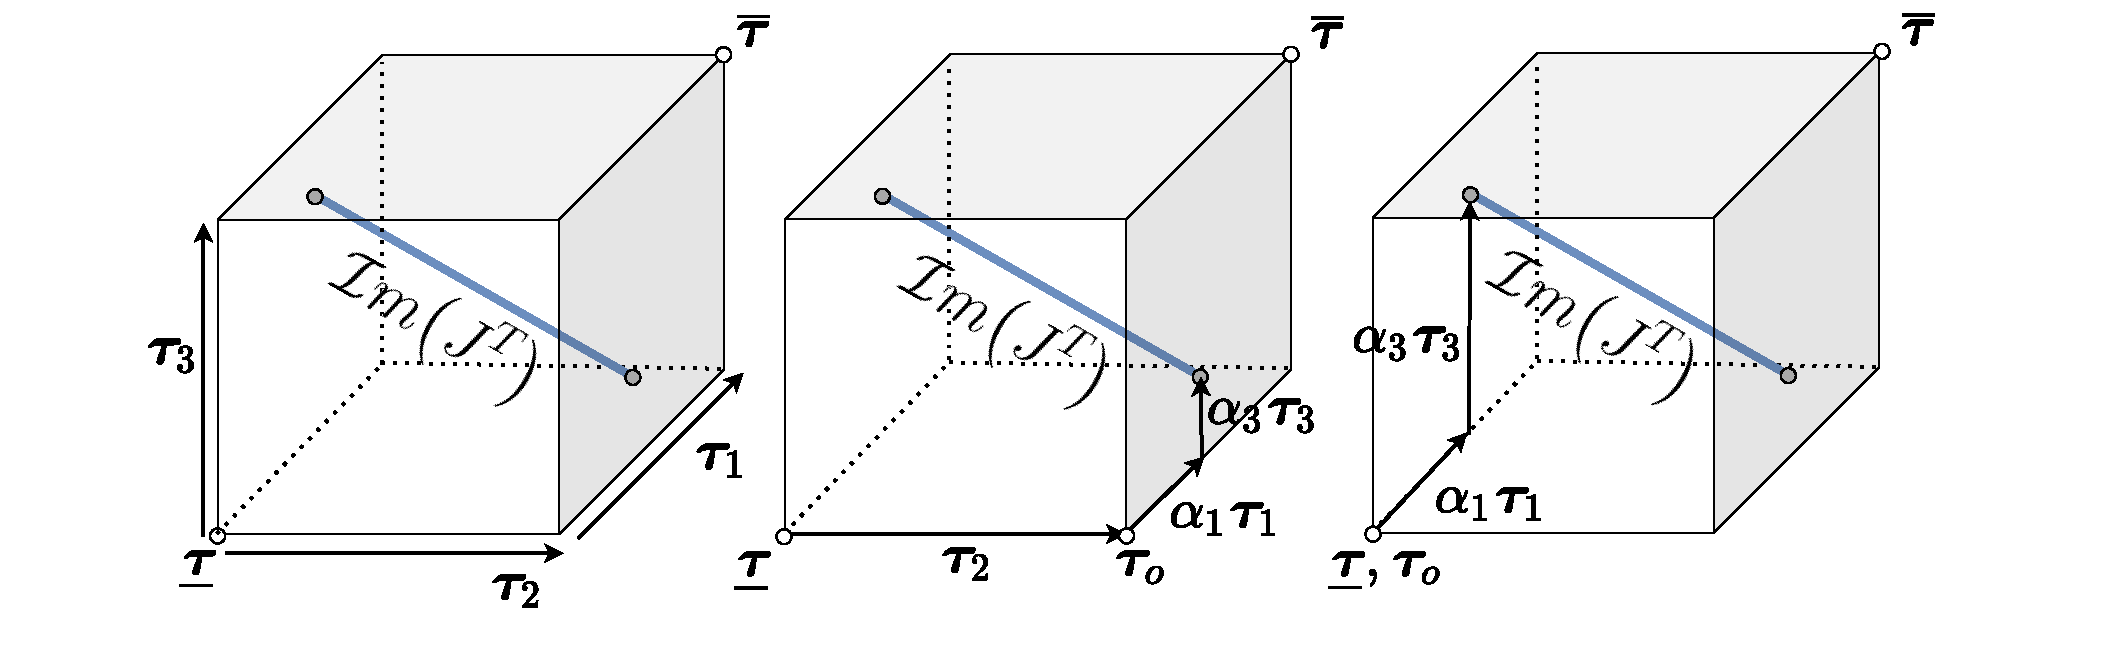
\includegraphics[width=1.1\linewidth]{Papers/images/intersection_example.pdf}
    \caption{Example of joint space interpretation of the vertex search algorithm solution for $n$=$3$ and $m$=$1$. }
    \label{fig:intersection_example}
    \vspace*{-0.3cm}
\end{figure}

An $n$-dimensional parallelotope has $\big(\begin{smallmatrix}n\\m\end{smallmatrix}\big)$ sets of $2^m$ parallel $n$-$m$ dimensional faces. Each set of parallel faces can be represented with the linear combination of the same set of $n$-$m$ base vectors $\bm{\tau}_i$ or in other words with a set of $n$-$m$ scalars $\alpha_i$. The remaining $m$ scalars are set either to 0 or 1 and define the origin $\bm{\tau}_o$ of  each one of the $2^m$ faces from the set
\begin{equation}
    \bm{\tau}_o = \unum{\bm{\tau}} + \alpha_1 \bm{\tau}_1+ ... + \alpha_m \bm{\tau}_m
\end{equation} 
Therefore, each $n$-$m$ dimensional face can be reached by partitioning $\bm{\alpha} = \left[\bm{\alpha}_1^T ~\bm{\alpha}_2^T\right]^T$, $\bm{\alpha}_1$ containing $m$ scalars $\alpha_i$ fixed to $0$ or $1$ and $\bm{\alpha}_2$ containing the remaining $n$-$m$ scalars which define the linear combination of $n$-$m$ base vectors $\bm{\tau}_i$.

Figure \ref{fig:intersection_example} illustrates the case where $\mathcal{I}m(J^T)$ is a line in joint space. In this case the intersection space is $n$-$m$=$2$ dimensional. In this case, two scalars $\alpha_1$ and $\alpha_3$ are enough to characterise both vertices of interest with $\alpha_2$ fixed to $0$ or $1$.

In order to find the vertices of the force polytope $\mathcal{P}_f$, equations (\ref{eq:force}) and (\ref{eq:torque_new}) are combined to restrict the search to the set of torques $\bm{\tau} \in \left\{[\bm{\unum{\tau}},\bm{\onum{\tau}}] \cap \mathcal{I}m(J^T)\right\}$
\begin{equation}
    J(\bm{q})^T \bm{f}_{vert} = \unum{\bm{\tau}} + \alpha_1 \bm{\tau}_1+ \alpha_2 \bm{\tau}_2 + ... + \alpha_n \bm{\tau}_n \label{eq:inter_im_bounds_torque}
\end{equation}
For each $\left(\begin{smallmatrix}n\\m\end{smallmatrix}\right)$ combination of the $m$ scalars, $2^m$ values of $\bm{\tau}_o$ can be calculated. For each possible value of $\bm{\tau}_o$, a linear system deriving from equation~(\ref{eq:inter_im_bounds_torque}) can be solved to find the $n$-$m$ scalars $\bm{\alpha}_{2}$ and the corresponding force polytope vertex $\bm{f}_{vert}$
\begin{equation}
    \underbrace{\begin{bmatrix}J(\bm{q})^T&-\bm{\tau}_{m}_{+1} \, \dots \, -\bm{\tau}_{n} \end{bmatrix}}_{Z_{n\times n}} \begin{bmatrix}\bm{f}_{vert}\\ \alpha_{m+1} \\ \vdots\\\alpha_{n} \end{bmatrix} = \bm{\tau}_o
    \label{eq:linear_system_full}
\end{equation}
If $Z$ is invertible and if $\bm{\alpha}_2 \in [\bm{0},\bm{1}]$, $\bm{f}_{vert}$ is a vertex of the polytope $\mathcal{P}_f$
\begin{equation}
   \begin{bmatrix}\bm{f}_{vert}\\ \bm{\alpha}_{2} \end{bmatrix} = Z^{-1}\bm{\tau}_L, \quad  \bm{\alpha}_{2} \in [\bm{0},\bm{1}]
    \label{eq:linear_system_full_solution}
\end{equation}

Overall, in order to navigate all possible combinations of the $n$-$m$ dimensional faces which may contain vertices of the force polytope $\mathcal{P}_f$, $\big(\begin{smallmatrix}n\\m\end{smallmatrix}\big)$=$\frac{n!}{m!(n-m)!}$ inversions of $Z$ and  $2^m \frac{n!}{m!(n-m)!}$ checks that $\bm{\alpha}_2 \in [\bm{0},\bm{1}]$ have to be performed.

In the case depicted in figure \ref{fig:intersection_example} ($n$=$3$, $m$=$1$), $Z$ is inverted only $\big(\begin{smallmatrix}3\\1\end{smallmatrix}\big)$=$3$ times and conditions are evaluated 6 times, which exactly corresponds to the number of faces of the parallelotope. Taking the example of the 3DoF planar robot ($n$=$3$, $m$=$2$) the number of $Z$ inversions is 3 and the number of condition evaluation is 12, which exactly corresponds to the number of edges of the parallelotope. One of the nice features of this approach is that it does not require an explicit inversion of $J(\bm{q})^T$ as in equation~(\ref{eq:compute_vert}) to actually obtain the set of vertices composing $\mathcal{P}_f$.  
% \todo[inline]{Insist maybe that with this approach there is no need to do pseudo-inverse of jacobian and we obtain forces directly. An elegant way.}

\subsection{Improvement using the SVD}

In order to further improve the efficiency of the proposed algorithm the Singular Value Decomposition (SVD) \cite{klema_singular_1980} of $J(\bm{q})$ is used
\begin{equation}
     J(\bm{q}) =  U  \underbrace{\begin{bmatrix}S & O_{m\times (n-m)}\end{bmatrix}}_{\Sigma}\underbrace{\begin{bmatrix}V_1^T \\ V_2^T \end{bmatrix}}_{V^T}
\end{equation}
where $S= diag( \sigma_1 \dots \sigma_m)$ is a diagonal matrix containing the $m$ singular values of $J(\bm{q})$. $V_1^T \in \mathbb{R}^{m \times n}$ projects the space of generalized torques onto the preimage of $\mathcal{I}m(J(\bm{q}))$ and $V_2^T \in \mathbb{R}^{n-m \times n}$ is a basis of $\mathcal{K}er(J(\bm{q}))$. $V_1^T$ and $V_2^T$ are orthogonal vector subspaces yielding $V_2^T V_1 = O$ and thus 
% Since image-space and null-space of the jacobian matrix are orthogonal, all the joint torque vectors $J(\bm{q})^T\bm{f}=\bm{\tau}$ that belong to the image-space of the jacobian matrix will have zero projection to the null-space:
\begin{equation}
    V_2^T J(\bm{q})^T\bm{f} = \bm{0}
\end{equation}
This allows to reduce (\ref{eq:linear_system_full}) to
\begin{equation}
    \underbrace{V_2^T\begin{bmatrix}-\bm{\tau}_{m}_{+1} \dots -\bm{\tau}_{n} \end{bmatrix}}_{T_{(n-m)\times (n-m)}} \bm{\alpha}_2 = V_2^T\bm{\tau}_o
    \label{eq:linear_system_svd}
\end{equation}
If $T$ is invertible, $\bm{\alpha}_2$ can be computed by
\begin{equation}
\bm{\alpha}_2 = T^{-1}V_2^T\bm{\tau}_o
\end{equation}
When the computed $\bm{\alpha}_2 \in [\bm{0},\bm{1}]$,  the corresponding force polytope vertex can be calculated as
\begin{equation}
    \bm{f}_{vert} = J(\bm{q})^{T+} \big( \unum{\bm{\tau}} + \alpha_1\bm{\tau}_{1} +\dots+\alpha_n\bm{\tau}_{n}\big)
\end{equation}

This new approach requires the calculation of the SVD and the Jacobian matrix pseudo-inverse $J(\bm{q})^{T+}$. Nevertheless, since the Jacobian transpose pseudo-inverse can be efficiently calculated from the SVD as $J(\bm{q})^{T+} = U\Sigma^{T+}V^T$
and since both the SVD and pseudo-inverse are calculated once and of all per algorithm run, the computation efficiency is greatly improved due to the matrix dimension reduction from $n$ to $(n-m)$ when inverting $T$ instead of $Z$.


\subsection{Matrix inverse condition}

Due to the constrained nature of $\bm{\alpha}_2$, it is possible to efficiently calculate some bounds ${\bm{t}_{ub}}$ and $\bm{t}_{lb}$ such that $T\bm{\alpha}  \in [\bm{t}_{lb}, \bm{t}_{ub}]$.
%, defining the interval of null-space projections of the vector $\bm{\tau}_o$.
These bounds are found by row-wise summing only positive and only negative elements $t_{ij}$ of  $T$
\begin{equation}
t_{i,lb} = \sum_j \max(t_{ij}, 0), \qquad
t_{i,lb} = \sum_j \min(t_{ij}, 0) 
\label{eq:bounds_condition}
\end{equation}

This creates a bounding box around the space defined with the vector $T\bm{\alpha}_2$. Therefore, one can conclude that if all the $2^m$ combinations of $\bm{\tau}_o \notin [\bm{t}_{lb}, \bm{t}_{ub}] $, the system (\ref{eq:linear_system_svd}) cannot have a solution which satisfies $\bm{\alpha}_2 \in [\bm{0},\bm{1}]$, and there is no need to invert $T$ to figure it out.
% \begin{equation}
%     \forall \bm{\tau}_o, \quad s.t.\quad \quad V_2^T\bm{\tau}_o \not\in [\bm{t}_{lb}, \bm{t}_{ub}] 
% \end{equation}

\subsection{Extension to residual polytopes}

When evaluating the capability of a robot, it is a common practice to take into consideration the joint torques necessary to compensate for gravity $\bm{\tau}_g = \bm{g}(\bm{q})$ \cite{wei_output_nodate} 
\begin{equation}
    J(\bm{q})^T \bm{f} = \bm{\tau} - \bm{\tau}_g
\end{equation}
Furthermore, the same can be done to include the effects of the robot dynamics. For a fixed-base, serial manipulator the dynamics can be written as
\begin{equation}
    M(\bm{q})\ddot{\bm{q}} + C(\dot{\bm{q}},\bm{q})\dot{\bm{q}} + \bm{g}(\bm{q}) = \bm{\tau} - J(\bm{q})^T \bm{f}
    \label{eq:full_dynamics}
\end{equation}
where $M$ and $C$ are respectively the mass and Coriolis-Centrifugal matrices. The residual joint torque vector $\bm{\tau}$ can then be expressed as
\begin{equation}
    J(\bm{q})^T \bm{f} = \bm{\tau} - \bm{\tau}_g  - \big(\underbrace{M(\bm{q})\ddot{\bm{q}} + C(\dot{\bm{q}},\bm{q})\dot{\bm{q}}) \big)}_{\bm{\tau}_{d}}
    \label{eq:force_dynamics}
\end{equation}

Finally, in many cases it is useful to evaluate the residual force ability of a robot already applying a certain nominal wrenches $\bm{f}_{n}$ which imply to generate joint torques $\bm{\tau}_{n}$
\begin{equation}
\bm{\tau}_{n} =  J(\bm{q})^T \bm{f}_{n}  
\end{equation}

The \textit{residual force polytope} \cite{ferrolho_residual_2020} corresponding to the  feasible space of Cartesian wrenches $\bm{f}$ that can be applied and rejected by the robot end-effector, taking into consideration the torque necessary to overcome gravity $\bm{\tau}_{g}$, robot dynamics $\bm{\tau}_{d}$ and any nominal joint torque $\bm{\tau}_{n}$, can be computed using algorithm~\ref{alg:main_algo} and the updated joint constraints
\begin{equation}
\begin{split}
    \unum{\bm{\tau}}' &= \unum{\bm{\tau}} - \bm{\tau}_g - \bm{\tau}_{d} - \bm{\tau}_{n}  \\ 
    \onum{\bm{\tau}}' &= \onum{\bm{\tau}}  - \bm{\tau}_g - \bm{\tau}_{d} - \bm{\tau}_{n}
    \label{eq:residual_constraints}
\end{split}
\end{equation}

% To include the influences of the gravity $\bm{\tau}_{g}$, dynamics of movement $\bm{\tau}_{d}$ and applied nominal wrenches $\bm{\tau}_{n}$, the joint constraints (\ref{eq:constraints_f}) become
% \begin{equation}
% \begin{split}
%     \unum{\bm{\tau}}' &= \unum{\bm{\tau}} - \bm{\tau}_g - \bm{\tau}_{d} - \bm{\tau}_{n}  \\ 
%     \onum{\bm{\tau}}' &= \onum{\bm{\tau}}  - \bm{\tau}_g - \bm{\tau}_{d} - \bm{\tau}_{n}
%     \label{eq:residual_constraints}
% \end{split}
% \end{equation}

% The feasible space of Cartesian wrenches $\bm{f}$ that can be applied and rejected by robot end-effector, taking into consideration the torque necessary to overcome gravity $\bm{\tau}_{g}$, robot dynamics $\bm{\tau}_{d}$ and any nominal joint torque $\bm{\tau}_{n}$ is called \textit{residual force polytope} \cite{ferrolho_residual_2020}. 

\begin{algorithm}[!h]
\caption{New vertex search algorithm pseudo-code}
\begin{algorithmic}
\REQUIRE $J$, $\onum{\bm{\tau}}$, $\unum{\bm{\tau}}$ (Eq. \ref{eq:constraints_f} or Eq. \ref{eq:residual_constraints}) 
\STATE $U, \Sigma, V^T \leftarrow svd(J)$ 
\STATE $J^{T+} = U\Sigma^{T+}V^T$
\STATE $V_1,\, V_2  \leftarrow V $
\STATE calculate $n$ base vectors $\bm{\tau}_1 \dotsc \bm{\tau}_n$ (Eq. \ref{eq:torque_new})

\FORALL{  $\big(\begin{smallmatrix}n\\m\end{smallmatrix}\big)$ combinations of $m$ fixed $\alpha_i$ } 
\STATE construct $T$ matrix (Eq. \ref{eq:linear_system_svd})
\STATE find bounds $\bm{t}_{lb},\bm{t}_{ub}$ (Eq. \ref{eq:bounds_condition})

\FORALL{   $2^m$ vectors $\bm{\tau}_o$ } 
\IF{$ V_2^T\bm{\tau}_o \in [\bm{t}_{lb},\bm{t}_{ub}] $}
\STATE $\bm{\alpha}_2 = T^{-1}V_2^T\bm{\tau}_o $
\IF{$ \bm{\alpha}_2 \in [0,1] $}
\STATE $\bm{\tau}_{vert} = \unum{\bm{\tau}} + \alpha_1{\bm{\tau}_{1}} +\dots+\alpha_n{\bm{\tau}_{n}}$
\STATE $\bm{f}_{vert} = J^{T+}\bm{\tau}_{vert}$
\ENDIF
\ENDIF
\ENDFOR
\ENDFOR

\end{algorithmic}
\label{alg:main_algo}
\end{algorithm}

\section{Complexity analysis}\label{sec:complexity}
To demonstrate the efficiency of the proposed polytope vertex search algorithm, it is compared to the polytope vertex search algorithm introduced by Chiacchio et al. \cite{chiacchio_evaluation_1996}. Furthermore the comparison is extended to the algorithm proposed by Sasaki et al. \cite{sasaki_vertex_nodate} which is, to our knowledge, the only algorithm exploiting the geometric structure of the problem.


% \begin{table*}[!b]
%     \centering
%     \caption{Complexity and execution time comparison for three vertex search algorithms in general case, for  4 DOF planar robot, 6DOF and 7DOF collaborative robots}
%     \begin{tabular}{r | r |c | c | c}
%       \toprule
%       \textbf{Robot} & \textbf{Metric} & \textbf{Chiacchio}\cite{chiacchio_evaluation_1996} & \textbf{Sasaki} \cite{sasaki_vertex_nodate}  &  \textbf{Our approach} \\
%       \hline
%       $\smash{n,m}$& matrix inv. & $ \frac{2n!}{m!(2n-m)!}$ & $ \frac{n!}{m!(n-m)!} $ & $ \leq \frac{n!}{m!(n-m)!}$ \\
%       & matrix dim.  & $ 2n \times 2n$ & $ m\times m $ & $n$-$m$ $\times$ $n$-$m$\\
%       & time[ms] & & & \\
%       \hline
%       \textit{4 link} &  matrix inv. & 24 & 6 & 4.2 $\pm$ 1.4 (6) \\ 
%         $n$=$4$&matrix dim.  & 8x8 & 2x2 & 2x2 \\ 
%       $m$=$2$& time[ms] & 2.7 $\pm$ 0.1 (3.6) & 0.93 $\pm$ 0.1 (1.1) & 0.64 $\pm$ 0.1 (1.5) \\ 
%       \hline
%       \textit{UR5} &  matrix inv. & 220 & 20 & 2.8 $\pm$ 2.5 (10) \\ 
%         $n$=$6$&matrix dim.  & 12x12 & 3x3 & 3x3 \\ 
%       $m$=$3$& time[ms] & 14.2 $\pm$ 0.9 (20) & 2.1 $\pm$ 0.2 (3.4) & 1.5 $\pm$ 0.2 (2.7) \\ 
%       \hline
%       \textit{Panda} &   matrix inv.  &  364 & 35 & 7.3 $\pm$ 4.2 (20)\\
%       $n$=$7$ & matrix dim.  &  14x14 & 3x3 & 4x4\\
%       $m$=$3$&time[ms]  &  25 $\pm$ 0.5 (27) & 3.5 $\pm$ 0.1 (5.4) & 2.6 $\pm$ 0.2 (4.3)\\
%       \bottomrule
%     \end{tabular}
%     \label{tab:complexity_results}
% \end{table*}




The three algorithms have been tested to find vertices of the force polytope $\mathcal{P}_f$ for three different robots: a 4R planar robot ($n$=$4$,$m$=$2$), the \textit{Universal Robots} UR5 6DoF robot ($n$=$6$,$m$=$3$) and the \textit{Franka Emika Panda} 7DoF robot ($n$=$7$,$m$=$3$). The results are averaged over 1000 randomly selected robot configurations. All algorithms have been implemented in the programming language Python and tested on a laptop equipped with a 1.90GHz Intel i7-8650U processor. The code of the proposed algorithm is publicly available\footnote{ \url{https://gitlab.inria.fr/askuric/polytope\_vertex\_search}}.

Table \ref{tab:complexity_results} shows the results of this complexity evaluation. The proposed vertex search algorithm drastically reduces the number of matrix inversions and thus reduces the processing time considerably: $4$-$10\times$ faster execution than Chiacchio's algorithm and on average 20\% faster than Sasaki's. Results show that even for the cases of 6DoF and 7DoF industrial robots our approach is capable of evaluating the polytope vertices under $3ms$. Such a low processing time opens numerous opportunities for the on-line use of polytope based capacity evaluation especially in the area of robot control.

\begin{table}
    \centering
    \caption{Complexity and execution time (in milliseconds) comparison for three different vertex search algorithms. For each algorithm, 3 robots are tested. The provided results are averaged over 1000 randomly picked robot configurations. They are provided in terms of number of matrix inversions, inverted matrix size and time of execution.}
    \begin{tabular}{|l|c|c|c|}
       \hline
       Robot & \textbf{Chiacchio}\cite{chiacchio_evaluation_1996} & \textbf{Sasaki} \cite{sasaki_vertex_nodate}  &  \textbf{Proposed} \\
       \hline
       $(n,m)$& mat.inversions: $ \frac{2n!}{m!(2n-m)!}$  & $ \frac{n!}{m!(n-m)!} $ & $ \leq \frac{n!}{m!(n-m)!}$ \\
       &  mat. size:  $ 2n \times 2n$ & $m\times m$  & $n$-$m$ $\times$ $n$-$m$\\
       & time[ms]: t $\pm$ sd (max) & & \\
       \hline
       $(4,2)$ &  24 & 6 & 4.2$\pm$1.4 (6) \\ 
       & 8$\times$8 & 2$\times$2 & 2$\times$2 \\ 
       & 2.7$\pm$0.1 (3.6) & 0.93$\pm$0.1 (1.1) & 0.64$\pm$0.1 (1.5) \\ 
       \hline
       $(6,3)$ & 220 & 20 & 2.8$\pm$2.5 (10) \\ 
        & 12$\times$12 & 3$\times$3 & 3$\times$3 \\ 
       & 14.2$\pm$0.9 (20) & 2.1$\pm$0.2 (3.4) & 1.5$\pm$0.2 (2.7) \\ 
       \hline
      $(7,3)$&    364 & 35 & 7.3$\pm$4.2 (20)\\
        & 14$\times$14 & 3$\times$3 & 4$\times4$\\
       & 25$\pm$0.5 (27) & 3.5$\pm$0.1 (5.4) & 2.6$\pm$0.2 (4.3)\\

       \hline
    \end{tabular}
    \label{tab:complexity_results}
\end{table}


\section{Discussions}
\label{sec:discussion}
In this section, the potential of applying the on-line capacity evaluation for collaborative robots and the human-robot interaction is discussed.


\subsection{Polytopes for multi-robot systems}
\begin{figure}[!h]
    \centering
    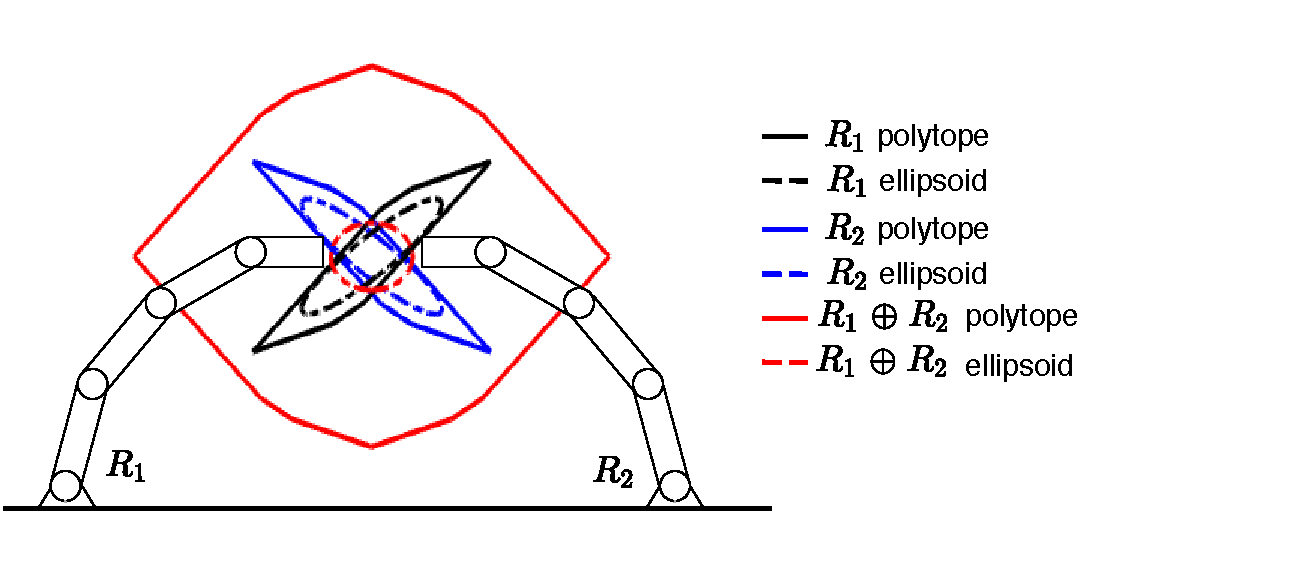
\includegraphics[width=\linewidth]{Papers/images/collaborative_difference.pdf}
    \caption{4DoF planar robots collaboration: polytopes and ellipsoids. Link lengths $l_i$$=$$0.5$, torque limit $|\tau_i|$$<$$1$ and joint angles $q_i$$=$$-\pi/8$ for $R_1$ and $q_i$$=$$\pi/8$ for $R_2$.}
    \label{fig:collaborative_difference}
\end{figure}

Up to recently \cite{long2020constrained}, the estimation of task-space capabilities of multiple robotic manipulators was largely depending on manipulability ellipsoids \cite{chiacchio_task_1991}\cite{chiacchio_global_1991}\cite{lee_dual_1989}.

However as the number of robots grows, the ellipsoid approach, which rely on a Euclidean norm rather than an infinity norm \cite{merlet_jacobian_2006}, provides a less accurate approximation and the question of what is the best practice to sum \cite{chiacchio_task_1991}\cite{julio_frantz_analysis_2015} or intersect \cite{sekiguchi_force_2017}\cite{lee_dual_1989} multiple ellipsoids becomes problematic. 

Figure \ref{fig:collaborative_difference} shows one example of two collaborating 4DoF planar robots joint force capacity based on ellipsoids and polytopes.  The ellipsoids are calculated using the approach proposed by Chiacchio \cite{chiacchio_task_1991} and the joint polytope is calculated as the Minkowski sum of the individual force polytope of each robot.
\begin{equation}
\mathcal{P}_{f_\oplus} = \mathcal{P}_{f_{R_1}} \oplus \mathcal{P}_{f_{R_2}} 
\end{equation}
This example clearly demonstrates that even though ellipsoids can reasonably well provide an approximation of the force capacity of each robot separately, the same is not the case for the capacity of the dyad.

A similar conclusion can be drawn for use cases where the joint capacity of multiple robots can be represented by the intersection of their polytopes \cite{long2020constrained}, \texit{i.e} when the robots are working in opposition, both applying a similar force $\bm{f}$ in opposite directions\footnote{A typical example of this situation is the case of the frictional grasp of an object.}
\begin{equation}
\mathcal{P}_f = \mathcal{P}_{f_{R_1}}  \cap \mathcal{P}_{f_{R_2}}     
\end{equation}
In that case, the polytope intersection problem can be elegantly transformed into the vertex enumeration problem for the extended system
\begin{equation}
J_\cap = [J_{R_1}\, J_{R_2}],\quad \bm{\tau} = \left[\bm{\tau}_{R_1}^T\, \bm{\tau}_{R_2}^T\right]^T, \quad J_\cap^T\bm{f} = \bm{\tau}
\end{equation}

\subsection{Polytopes for human-robot collaboration}
Several authors have studied the use of robotics performance measures such as manipulability ellipsoids and polytopes for human arms using 7DoF manipulator models \cite{rezzoug_application_2012}\cite{lazinica_higher_2010}\cite{carmichael_estimating_2013}\cite{carmichael_towards_2011} or full musculoskeletal model \cite{hernandez_toward_2015}. A promising approach for leveraging the efficient on-line polytope evaluation algorithm is to estimate the joint capacity of the robot and human and adapt the robotic assistance as a function of the evolution of human capabilities.  One of the associated challenges is to extend the proposed vertex search algorithms to actuation constraints which result from more complex actuation mechanisms such as muscles and can thus no longer be represented as parallelotopes.

\section{Conclusion}

The proposed vertex search algorithm provides a computationally efficient tool for the polytope-based, online evaluation of task-space robot capabilities. As illustrated in this work, the ability to accurately evaluate on-line the capabilities of robots leverages several possibilities in modern robotic applications where oversizing robots is no longer an option.




% \section{Conclusion}
% In this paper we presented a new real-time capable polytope vertex finding algorithm for efficient calculating twist and wrench polytopes. The new algorithm is capable of calculating polytope vertices for 6DOF and 7DOF robots under 3ms. An experimental setup with two collaborating \textit{Franka Amika Panda} robots has been created to demonstrate the algoritm potential. By leveraging the real force capacity evaluation we created a simple control strategy to safely carry the mass of 12 kilograms.

% 

\chapter{Force capacity polytope algorithm for humans}

%%%%%%%%%%%%%%%%%%%%%%%%%%%%%%%%%%%%%%%%%%%%%%%%%%%%%%%%%%%%%%%%%%%%%%%%%%%%%%%%
Many recent human-robot collaboration strategies, such as \textit{Assist-As-Needed} (AAN), are promoting human-centered robot control, where the robot continuously adapts its assistance level based on the real-time need of its human counterpart.
One of the fundamental assumptions of these approaches is the ability to measure or estimate the physical capacity of humans in real-time.

In this work, we propose an algorithm for the feasibility set analysis of a generic class of linear algebra problems. This novel iterative convex-hull method is applied to the determination of the feasible cartesian wrench polytope associated to a musculoskeletal model of the human upper limb. The method is capable of running in real-time and allows the user to define the desired estimation accuracy.  
The algorithm performance analysis shows that the execution time has near-linear relationship to the considered number of muscles, as opposed to the exponential relationship of the conventional methods. Finally, real-time robot control application of the algorithm is demonstrated in a \textit{Collaborative carrying} experiment, where a human operator and a \textit{Franka Emika Panda} robot jointly carry a 7kg object. The robot is controlled in accordance to the AAN paradigm maintaining the load carried by the human operator at 30\% of its carrying capacity.

%%%%%%%%%%%%%%%%%%%%%%%%%%%%%%%%%%%%%%%%%%%%%%%%%%%%%%%%%%%%%%%%%%%%%%%%%%%%%%%%
\section{Introduction}

The number of collaborative robots, robots designed to closely coexist with humans, is increasing exponentially in recent years \cite{ajoudani2018progress}, paving the way for more comprehensive and human-centered solutions for human robot collaboration. However, due to the instantaneous nature of the physical interaction, it becomes increasingly challenging to design and tune control laws for the collaborative systems \textit{a priori}. Accounting, in advance, for the high degree of variability induced by humans, usually results in very conservative safety limits and reduces the overall collaboration efficiency considerably. Therefore, new on-line capable and accurate metrics are needed to improve performance of the collaborative systems while ensuring safety for all humans involved. \textit{Assist-As-Needed} (AAN)\cite{carmichael2013admittance} is one recent example of such paradigm, where a robot continuously adapts the assistance level taking in consideration the capacity of the human operator in real-time.

Several capacity metrics have been developed over the years, first by the robotics community\cite{yoshikawa1985manipulability}\cite{chiacchio_evaluation_1996}, and later adapted to the human motion analysis\cite{sasaki2011vertex}\cite{khatib2009robotics}\cite{biomechanics1010008}. The most well known representatives being wrench, twist and acceleration capacity. While twist and acceleration capacity represent the level of dexterity in different directions, wrench capacity represents the human ability to apply and resist external wrenches in arbitrary directions, being very important both safety-wise and performance-wise. 

\begin{figure}[!t]
    \centering
   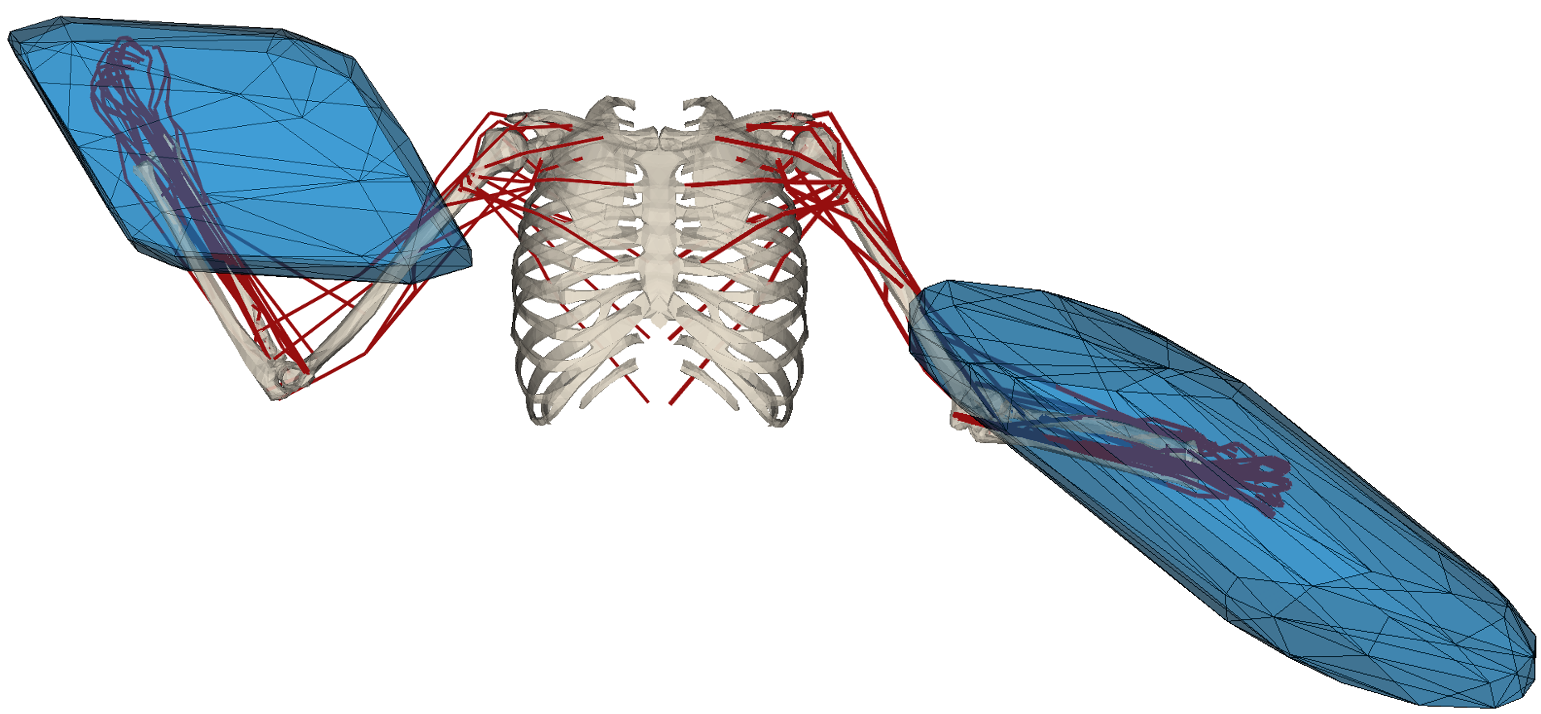
\includegraphics[width=0.9\linewidth]{Papers/images/bimanual.png}
    \caption{Cartesian force polytope of a musculoskeletal model of both human upper limbs  \cite{saul2015benchmarking} with 7Dof and 50 muscles each, visualised in \textit{pyomeca bioviz} \cite{Michaud2021}. The polytopes are scaled with a ratio 1m : 1000N}
   \label{fig:polytope_showoff}
\end{figure}

The human body capacities are governed by many different factors \cite{nasa}. Many of them are physiological and biomechanical factors, such as muscle strength, bone length and level of fatigue. The others are purely kinematic such as posture, joint velocities and accelerations. 
Among the most complete human body modeling approaches are the musculoskeletal models, describing the relationship between the activation of human muscles and the body dynamics. 
Over the years, many, more or less complete, models have been developed and experimentally validated \cite{holzbaur2005model}\cite{WU20163626}\cite{rajagopal2016fullbody}, as well as different open-source software platforms created for their analysis \cite{opensim}\cite{Michaud2021}. 

The exact wrench, twist and acceleration capacity of the musculoskeletal model can be represented in a form of convex polytopes. However due to the relatively high number of muscles usually considered, the exact evaluation of these polytopes is a time consuming process. Therefore, in order to reduce the complexity of their calculation, apart from using less complex models, various approximate techniques have been proposed, using machine learning \cite{hernandez2018force}, ellipsoids \cite{petric2019assistive} and approximate polytope estimation techniques \cite{carmichael2011Towards}\cite{chen2018strength}.  However, all of these approaches reduce the precision and confidence in the calculated human capacity. 

In this paper, a new algorithm for polytope evaluation is proposed. It allows for the efficient evaluation of the feasible wrench polytope of musculoskeletal human models, given a user specified accuracy. The efficiency is characterized by the low and near-linear complexity with respect to the number of muscles and accuracy. This allows for an online update of the polytope at a rate of 100 ms \antun{ (10 Hz)} for 32 muscles and an accuracy of 5 N \antun{(200 ms / 5 Hz for 50 muscles)}. Beyond these application specific characteristics, the proposed algorithm is generic to a class of implicitly defined linear algebra feasibility problems
\begin{equation}
    A\bm{x} = B\bm{y},\quad  \bm{y}\in \left[\unum{\bm{y}}, \onum{\bm{y}}\right]
    \label{eq:eq_general}
\end{equation}
where 
\begin{equation}
   \bm{x} \in \mathbb{R}^m, ~\bm{y} \in \mathbb{R}^d, ~A\in\mathbb{R}^{n \times m}, ~B\in\mathbb{R}^{n \times d}, ~ d\geq n \!\geq\! m
\end{equation}
In robotics, this class of problems can be found in many different domains such as when calculating feasible twist capacity of object grasping \cite{Prattichizzo2016}, feasible twist capacity of collaborating robots forming a closed chain \cite{bicchi2000manipulability}, or feasible wrench capacity of multilink cable driven parallel robots \cite{lau2016caspr}\cite{sheng2020operational}. %In the context of this paper, the proposed algorithm is used for feasible wrench polytope evaluation of musculoskeletal models. 
%Additionally, similar analysis can be done for the velocity and acceleration capacity as well.

Section \ref{ch:problem_formualtion} recapitulates the mathematical formulation of the feasible wrench polytope for musculoskeletal models, followed by the description of the proposed algorithm in Section \ref{ch:algorihtm}. In Section \ref{ch:results} the performance characteristics of the algorithm are analysed and compared with state of the art methods. Finally, a demonstrative experiment is shown where the proposed algorithm is used for real-time collaborative robot control. 


\section{Feasible wrench polytopes formulation}
\label{ch:problem_formualtion}
The dynamical equation of a general musculoskeletal system expressed in joint space can be formulated as
\begin{equation}
    \underbrace{M(\bm{q})\ddot{\bm{q}} + C(\bm{q},\dot{\bm{q}})\dot{\bm{q}}}_{\bm{\tau}_d} + \bm{\tau}_g(\bm{q}) = \bm{\tau} - J^{T}(\bm{q})\bm{f}  
    \label{eq:human_dynamics}
\end{equation}
where $\bm{q},\dot{\bm{q}},\ddot{\bm{q}} \in \mathbb{R}^n $ are the joint level generalised coordinates, velocities and accelerations. $M$ is the inertia matrix, $C$ is the Coriolis-centrifugal matrix, $\bm{\tau}_g$ is the joint torque produced by gravity, $\bm{\tau}$ is the joint torque vector generated by the muscle-tendon units, $J$ is the end effector Jacobian matrix and $\bm{f} \in \mathbb{R}^m$ is an $m$-dimensional external Cartesian wrench vector. $\bm{\tau}_d$ represents the joint torques induced by the body motion, kineto-static conditions $\dot{\bm{q}}\!=\!\ddot{\bm{q}}\!=\!0$ yield $\bm{\tau}_d = 0$.  
\begin{equation}
    \bm{\tau} - \bm{\tau}_d(\bm{q},\dot{\bm{q}},\ddot{\bm{q}}) - \bm{\tau}_g(\bm{q}) =  J^{T}(\bm{q})\bm{f}
    \label{eq:human_dynamics2}
\end{equation}

From equation (\ref{eq:human_dynamics2}), it can be seen that the gravity and body motion directly reduce the capacity to resist and apply external forces. 
%However, in many cases the gravitational and dynamical effects can be neglected $\bm{\tau}_g\!=\!\bm{\tau}_d\!=\!0$ considering only the influence of muscular forces to the Cartesian force generation
% \begin{equation}
%     \bm{\tau} =  J^{T}(\bm{q})\bm{f}
%     \label{eq:human_simple}
% \end{equation}

\subsection{Muscle model}
The joint torque $\bm{\tau}$ is generated by muscle-tendon units. One of the most well known muscle models was introduced by A. Hill \cite{hill1938heat} and later refined by F. Zajac \cite{zajac1989muscle}, where the muscle is approximated by a tensile force composed of an active and a passive component
\begin{equation}
    F_i = f^A_i(l_i,v_i)F_{iso,i} \alpha_i + \underbrace{f^P_{i}(l_i)F_{iso,i}}_{F_{p,i}}, \quad \alpha_i \in \left[0, 1\right]
\end{equation}

$f^A_{i}$ and $f^P_{i}$ are active and passive scaling functions depending on the muscle length $l_i$ and contraction/extension velocity $v_i$. $F_{iso,i}$ is the maximal isometric force the muscle can generate and $\alpha_i$ is the muscle activation level. For a set of $d$ muscles, with specified muscle lengths $\bm{l}$ and contraction velocities $\bm{v}$ the achievable set of muscle tensile forces $\bm{F} \in\mathbb{R}^d$ has a range
\begin{equation}
    \bm{F} \in \left[ \bm{F}_{p}, ~ \bm{F}_m\right]
    \label{eq:muslce_initial_range}
\end{equation}
\antun{where $\bm{F}_p$ is the vector of passive forces obtained for $\bm{\alpha}\!=\!0$ and $\bm{F}_m$ is the maximal muscle force vector obtained for $\bm{\alpha}\!=\!1$. 

\begin{equation}
\begin{aligned}
    F_{p,i} &= f^P_i(l_i)F_{iso,i}\\
    F_{m,i} &= \left(f^A_i(l_i,v_i) + f^P_i(l_i)\right)F_{iso,i}
\end{aligned}
\end{equation}}
%NR, typo : $f^P_i(l_i)$ depends only on $l_i$
The joint torque $\bm{\tau}$, generated by the muscle tensile force $\bm{F}$, can then be calculated using the Moment arm matrix \cite{pandy1994}   
\begin{equation}
    \bm{\tau} = -L^{T}(\bm{q})\bm{F} 
    \label{eq:muscle_torqe_gen}
\end{equation}
where $L(\bm{q})^T$ is the transpose of the moment arm matrix, which \antun{corresponds to} the muscle length Jacobian relating the space of joint and muscle length velocities  
\begin{equation}
    \dot{\bm{l}} = L(\bm{q}) \dot{\bm{q}},\quad L_{ij}=\dfrac{\partial l_i}{\partial q_j}
\end{equation}
Finally, the negative sign in equation (\ref{eq:muscle_torqe_gen}) makes the force applied in the length shortening direction of the muscle positive. 

Combining equations (\ref{eq:human_dynamics2}) and (\ref{eq:muscle_torqe_gen}), one obtains the relationship relating the $d$ muscle tensile forces $\bm{F}$ and  the $m$ dimensional Cartesian wrench $\bm{f}$
\begin{equation}
    J^{T}(\bm{q})\bm{f} = -L^{T}(\bm{q})\bm{F} - \bm{\tau}_d(\bm{q},\dot{\bm{q}},\ddot{\bm{q}})- \bm{\tau}_g(\bm{q})
\end{equation}

\subsection{Residual muscle forces}
For any given joint configuration $\bm{q}$, velocity $\dot{\bm{q}}$ and acceleration $\ddot{\bm{q}}$, the dynamics $\bm{\tau}_d$ and the gravity $\bm{\tau}_g$ torques are constants and can be considered as a bias. Their equivalent bias muscle force $\bm{F}_{b}$ can be \antun{expressed as}
\begin{equation}
    -L^{T}(\bm{q})\bm{F}_{b} = \bm{\tau}_d(\bm{q},\dot{\bm{q}},\ddot{\bm{q}}) + \bm{\tau}_g(\bm{q})
    \label{eq:torque_constraint}
\end{equation}
This force $\bm{F}_{b}$ can be assessed by finding the minimal muscle activation $\bm{\alpha}$ that generates the desired torque vector \cite{ANDERSON2001153}. This can be resolved using a quadratic problem formulation where the muscle activation vector norm $||\bm{\alpha}||^2$ is minimised, with equation (\ref{eq:torque_constraint}) as equality constraint 
\begin{equation}
\begin{aligned}
    \min_{\bm{F_b}} \quad &  \frac{1}{2}\bm{F}_{b}^TP\bm{F}_{b}\\
     \textrm{s.t.} \quad &  -L^T\bm{F}_{b}= \bm{\tau}_g + \bm{\tau}_d \\
          & \bm{F}_{p} \leq \bm{F}_{b} \leq \bm{F}_{m} \\
\end{aligned}
\end{equation}
where  $P$ is a diagonal matrix with elements on diagonal $ p_{ii}=1/(F_{m,i}\! -\! F_{p,i})^2 $. 

Furthermore, the bias muscle forces $\bm{F}_{b}$ can then be used to \antun{calculate} the range of possible residual muscle forces $\bm{F}'$ from equation (\ref{eq:muslce_initial_range})

\begin{equation}
    \bm{F}' =  \bm{F} - \bm{F}_{b}, \quad \bm{F}' \in \left[\bm{0}, ~ \bm{F}_{m}\! -\! \bm{F}_{b} \right] 
\end{equation}

Finally, without loss of generality, the relationship of the muscle-tendon tension forces $\bm{F}$ and the Cartesian wrenches $\bm{f}$ can be expresses as
\begin{equation}
    J^{T}(\bm{q})\bm{f} = -L^{T}(\bm{q})\bm{F}, \quad \bm{F} \!\in\! \left[\unum{\bm{F}},\,\onum{\bm{F}}\right]
\end{equation}
where the $\unum{\bm{F}}$ and $\onum{\bm{F}}$ are the minimal and maximal muscle-tendon tension forces $\bm{F}$.

\subsection{Wrench capacity polytope}\label{ch:wrench_feasabiliy_definition}

A general achievable set of muscle-tendon tensile forces  $\bm{F}\!\in\!\left[\unum{\bm{F}},\,\onum{\bm{F}}\right] $ forms a $d$-dimensional hyper-rectangle 
with side lengths equal to the ranges of each of the $d$ muscle forces. Using the moment arm matrix $L(\bm{q})$ and equation (\ref{eq:muscle_torqe_gen}) this hyper-rectangle can be projected into the $n$-dimensional space of joint torques $\bm{\tau}$, forming the convex polytope of achievable joint torques $\mathcal{P}_\tau$
\begin{equation}
    \mathcal{P}_\tau = \big\{ \bm{\tau}\! \in\! \mathbb{R}^{n} ~ | ~ \bm{\tau} =\! -L^{T}(\bm{q})\bm{F}, ~ \bm{F}\! \in\! \left[\unum{\bm{F}},\,\onum{\bm{F}}\right] \big\}
    \label{eq:torque_poly}
\end{equation}

Furthermore, the dual relationship of the $m$-dimensional Cartesian wrenches $\bm{f}$ and the generalised joint torques $\bm{\tau}$ is given through the Jacobian transpose matrix $J^{T}(\bm{q})\bm{f}\! = \!\bm{\tau}$ and defines the achievable Cartesian force polytope
\begin{equation}
    \mathcal{P}_f = \big\{ \bm{f}\! \in\! \mathbb{R}^{m} ~ | ~ J^{T}(\bm{q})\bm{f}\! =\! \bm{\tau}, ~ \bm{\tau}\! \in\! \mathcal{P}_\tau \big\}
    \label{eq:force_poly_1}
\end{equation}

Combining the definitions (\ref{eq:torque_poly}) and (\ref{eq:force_poly_1}) the implicit definition of $\mathcal{P}_f$ can be defined as
\begin{equation}
    \mathcal{P}_f = \left\{ \bm{f}\! \in\! \mathbb{R}^{m} ~ | ~ J^{T}(\bm{q})\bm{f}\! =\! -L^{T}(\bm{q})\bm{F}, \bm{F}\! \in\! \left[\unum{\bm{F}},\,\onum{\bm{F}}\right]\right\}
    \label{eq:full_polytope}
\end{equation}

\begin{figure}[!t]
    \centering
    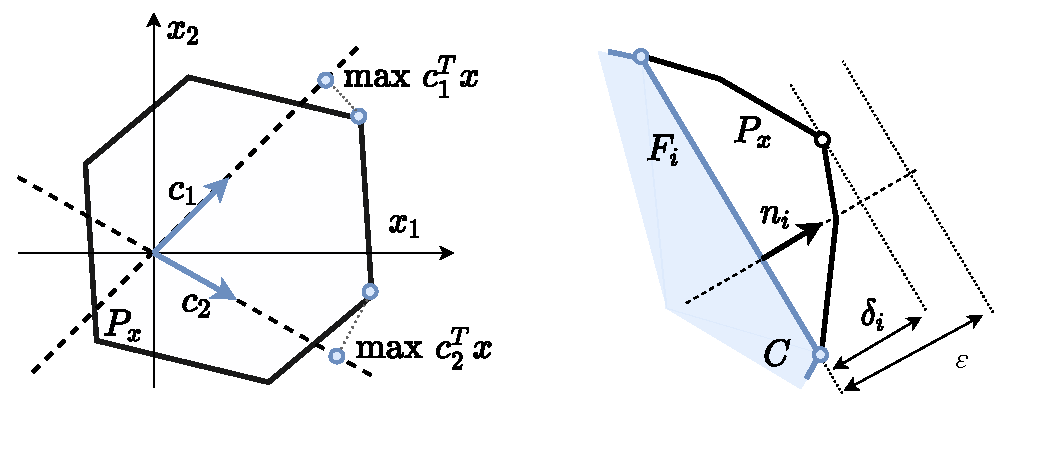
\includegraphics[width=0.90\linewidth]{Papers/images/poly_lp_vert_sample.pdf}
    \vspace{-0.2cm}
    \caption{Left figure demonstrates the LP based vertex search by choosing two different vectors $\bm{c}$. Right figure exemplifies the polytope face condition from equations (\ref{eq:normal_coplanar_test}) and (\ref{eq:normal_distance}), where  face $\mathcal{F}_i$ of the convex-hull $\mathcal{C}$ is considered to be the face of $\mathcal{P}_x$, because $\delta_i\! < \!\varepsilon$.  }
    \label{fig:sample_problems}
\end{figure}

\section{Polytope evaluation formulation}
\label{ch:algorihtm}

Given the generic formulation of problem (\ref{eq:eq_general}) the set of all feasible $\bm{x}$ forms a convex polytope 
\begin{equation}
    \mathcal{P}_x = \big\{ \bm{x}\in \mathbb{R}^{m}\, |\,A\bm{x} = B\bm{y},\quad  \bm{y}\in \left[\unum{\bm{y}}, \onum{\bm{y}}\right]  \big\}
    \label{eq:poly_init_2}
\end{equation}

%In the \ref{ch:lp_adapt}, new LP formation is proposed adapting it to the implicit formulation (\ref{eq:full_polytope}) of the polytope $\mathcal{P}_f$. In the section \ref{ch:method}, the proposed algorithm overview is given, as well as the pseudo-code and the geometrical representation.

The polytope evaluation can either be done by finding the set of all the vertices \antun{ ($\mathcal{V}$-rep)} or by finding its half-space representation \antun{($\mathcal{H}$-rep)}. Most of the commonly used polytope evaluation algorithms are very efficient for finding the exact solution to very specific problems: \cite{fukuda_dd}\cite{skuric:hal-02993408}\cite{sasaki2011vertex} calculate the $\mathcal{V}$-rep of $A\bm{x}\!=\!\bm{b},\bm{b}\!\in\![\bm{b}]$ and \cite{hyper_psm}\cite{dantzig1973fourier}\cite{jones2004equality} calculate the $\mathcal{H}$-rep of $\bm{x}\!=\! A\bm{y},\bm{y}\!\in\![\bm{y}]$. However since the number of faces and vertices of the polytopes augments exponentially with the size of the system, when the size of the problem becomes high, searching for the exact solution of the combined sub-problems becomes practically intractable \cite{Huynh2005PracticalIO}. 
%An example of such high-dimensional systems are the musculoskeletal models, where the number of muscles is usually large and even though the output space is low-dimensional Cartesian space the exact solution may take hours to calculate. 

To overcome this issue, various approximative approaches, such as the  \textit{Ray Shooting Method} (RSM)  \cite{agarwal1993ray} and the \textit{Convex-Hull Method} (CHM) \cite{lassez1992quantifier}, have been developed, reducing the complexity and improving the execution time. 
Although RSM algorithms are relatively simple to setup and have already been used for evaluating the capacity of musculoskeletal models \cite{carmichael2011Towards}, these algorithms do not provide any bound on their estimation error and highly rely on hand tuned initial parameters. 
CHM \cite{lassez1992quantifier} algorithms on the other hand, have shown to be very efficient while at the same time maintaining the bound of the user defined estimation error. CHM uses  \textit{linear-programming} (LP) repetitively to find new vertices and the convex-hull algorithm to group them to faces, augmenting the precision of the approximation successively. Additionally, CHM finds the $\mathcal{V}$-rep and the $\mathcal{H}$-rep of the polytope at the same time.  However in its standard formulation, the CHM is not suitable for the family of problems given with equation (\ref{eq:eq_general}). 

Therefore, Section \ref{ch:lp_adapt} introduces an LP formulation adapting the CHM approach to the implicit problem formulation (\ref{eq:eq_general}) and in Section \ref{ch:method}, the proposed algorithm overview is given, as well as the pseudo-code and the geometrical representation.


%The geometrical representation of solving the linear programming (LP) problem is finding a vertex of a polytope \cite{vajda_gass_1964}. However, in its implicit formation (\ref{eq:poly_init_2}) the polytope $\mathcal{P}_x$ is not suitable for the LP optimisation.




\subsection{Linear programming formulation}
\label{ch:lp_adapt}
From a geometrical point of view, solving a linear programming (LP) problem boils down to finding a vertex of a polytope \cite{vajda_gass_1964}. However, in order for the polytope $\mathcal{P}_x$ to be suitable for LP optimisation in the $m$-dimensional output space, its implicit formulation (\ref{eq:poly_init_2}) needs to be expressed in explicit form.

In the general case, $n\geq m$ and $A$ is not square. To find an explicit form of equation (\ref{eq:eq_general}), the pseudo-inverse $A^+$ can be used as a solution only if $B\bm{y}$ belongs to the \textit{image} of $A$ \cite{klema_singular_1980}. Therefore, equation (\ref{eq:eq_general}) can be transformed to 
\begin{equation}
    \bm{x} = A^{+} B \bm{y}, \quad B\bm{y} \in \mathcal{I}m(A)
    \label{eq:eq_general_red}
\end{equation} 
Using the \textit{Singular value decomposition} \cite{klema_singular_1980} of  $A = U\Sigma V^T$, an equality constraint can be devised for $B\bm{y}$ to belong to the \textit{image} of $A$
\begin{equation}
    U_2^TB\bm{y} = \bm{0}
    \label{eq:nullspace_gen}
\end{equation}
where rotation matrix $U \in \mathbb{R}^{n\times n }$ is separated into  $U_1\in \mathbb{R}^{n\times m}$, a projector to the  \textit{image} of $A$, and $U_2\in \mathbb{R}^{n\times(n-m)}$, a projector to its \textit{null-space}.

Finally, combining equations (\ref{eq:nullspace_gen}), (\ref{eq:eq_general_red}) and (\ref{eq:eq_general}), one can create a linear program \cite{vajda_gass_1964} capable of reaching all  vertices of the polytope $\mathcal{P}_x$
\begin{equation}
\begin{aligned}
    \max_{\bm{y}} \quad &  \bm{c}^TA^{+}B\bm{y} \\
     \textrm{s.t.} \quad &  U_2^TB\bm{y} = \bm{0} \\
          & \unum{\bm{y}} \leq \bm{y} \leq \onum{\bm{y}} \\
\end{aligned}
\label{eq:lin_prog}
\end{equation}
by appropriately choosing the projection $\bm{c}$, as demonstrated on figure \ref{fig:sample_problems}.


\subsection{Proposed algorithm overview}
\label{ch:method}

Given the polytope definition (\ref{eq:eq_general}) and (\ref{eq:poly_init_2}) and the LP problem defined in (\ref{eq:lin_prog}), the proposed method provides a structured way to choose vectors $\bm{c}$ to find all the vertices ($\mathcal{V}$-rep) and facets ($\mathcal{H}$-rep) of the polytope $\mathcal{P}_x$. 
In order to do so, the method leverages the iterative convex hull $\mathcal{C}$ calculation, where each newly found vertex extends $\mathcal{C}$. The normal vectors of the faces of the newly obtained $\mathcal{C}$ are used to decide for the new vectors $\bm{c}$ to use in the LP (\ref{eq:lin_prog}). This iterative process is performed until some specified level of accuracy is reached.

\begin{figure}[!t]
    \centering
    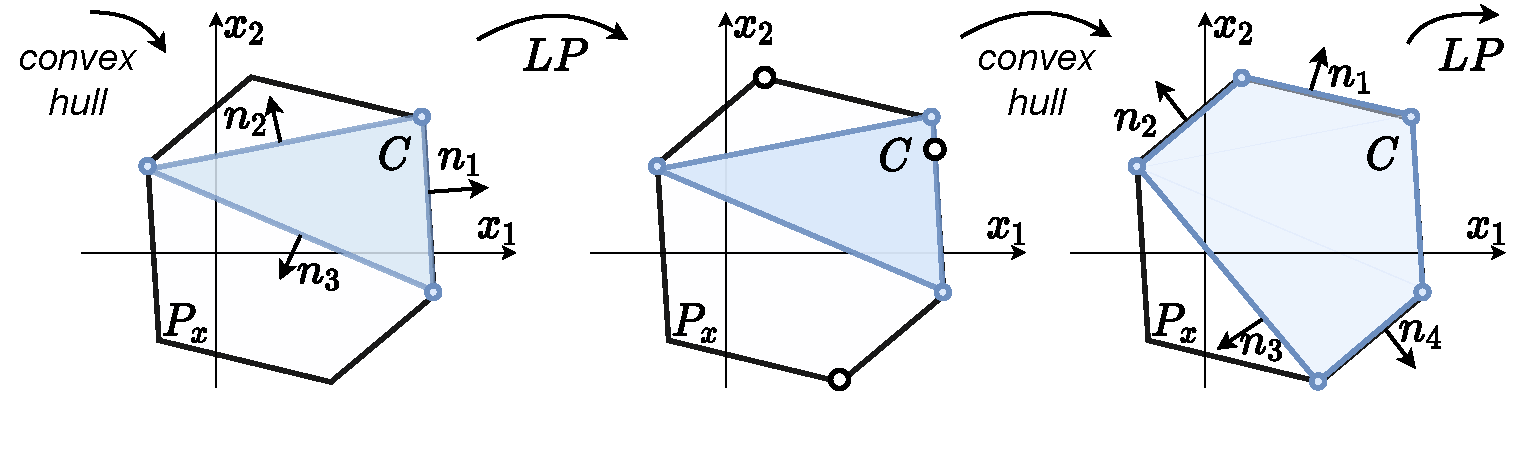
\includegraphics[width=\linewidth]{Papers/images/poly_lp_vert_part.pdf}
    \vspace{-0.8cm}
    \caption{This figure shows the procedure of successive approximation of the polytope $\mathcal{P}_x$ using the proposed CHM algorithm. The face normal vectors $\bm{n}_i$ of the convex-hull $\mathcal{C}$ are used with LP (\ref{eq:lin_prog}) to find new vertices which are then used to update the convex-hull $\mathcal{C}$ and furthermore improve the approximation of the polytope. }
    \label{fig:algo_example}
\end{figure}

More precisely, the first step of the algorithm constructs an initial set of vertices $\bm{x_v}$ and an initial convex hull. In a $m$-dimensional space, the minimal number of points to create a volume is $m\!+\!1$. Since $\bm{x}$, defined by relation (\ref{eq:eq_general_red}), can be expressed as a linear combination of the $m$ base vectors $v_i\in V$ of $A$, $$\bm{x} = a_0 \bm{v}_0 + \dots +a_m \bm{v}_m$$ a way to get the initial set of vertices is to solve LP (\ref{eq:lin_prog}) that minimises ($\bm{c} = -\bm{v}_i$) and maximises ($\bm{c} = \bm{v}_i$) the projection of the polytope $\mathcal{P}_x$ on the axes of each one of the base vectors $\bm{v}_i$. Once the initial set of vertices $\bm{x}_v$ is found, the initial convex hull $\mathcal{C}$ can be calculated. Its centroid position is given by $\bm{x}_c\!=\!\frac{1}{N}\!\sum\bm{x}_{v,i}$. 

The next step of the algorithm is to iterate over all the faces $\mathcal{F}_i$ of the convex hull $\mathcal{C}$. For each new face $\mathcal{F}_i$, the normal $\bm{n}_i$ is found and used as a candidate $\bm{c}_i$ in the direction pointing out of polytope $\mathcal{P}_x$.
%all the vertices $\bm{x}_{\mathcal{F}j}\! =\! %\bm{x}_v\!\in\!\mathcal{F}_i$. Then the $\bm{c}_i$ is defined %as normal $\bm{n}_i$ in the direction pointing out of the polytope 5$\mathcal{P}_x$.
The normal vector direction is verified by projecting the vector going from the centroid $\bm{x}_c$ to any vertex $\bm{x}_{j}$ of face $\mathcal{F}_i$, onto the normal $\bm{n}_i$ and verifying if the scalar product is positive or negative.
\begin{equation}
    \bm{c}_i = \begin{cases}
  \bm{n}_i, & \text{if } \bm{n}_i^T(\bm{x}_{j} - \bm{x}_c) \geq 0, \\
  -\bm{n}_i, & \text{otherwise}.
\end{cases} 
\label{eq:normal_condition}
\end{equation}

%NR why did you remove the variability of results, i think it was informative of the distribution of error of the RSM?

Solving equation (\ref{eq:lin_prog}) with $\bm{c}_i$, the obtained $\bm{x}_i$ can be either a vertex of the polytope $\mathcal{P}_x$ or be coplanar with face $\mathcal{F}_i$. To determine if  $\bm{x}_i$ is coplanar with the face, a simple check can be devised, which verifies if the orthogonal (normal) distance from $\bm{x}_i$ to any vertex $\bm{x}_{j}$ of face $\mathcal{F}_i$
\begin{equation}
    \delta_i = \bm{n}_i^T(\bm{x}_{j} - \bm{x}_i)
\label{eq:normal_distance}
\end{equation}
is within a certain user defined accuracy $\varepsilon$:
\begin{equation}
    \bm{x}_i = \begin{cases}
   \text{vertex}, & \text{if }  |\delta_i| \geq \varepsilon, \\
    \text{on the face}, & \text{otherwise}.
\end{cases} 
\label{eq:normal_coplanar_test}
\end{equation}
Figure \ref{fig:sample_problems} provides a graphical interpretation of this check and of the values $\delta_i$ and $\varepsilon$.

If $\bm{x}_i$ belongs to face $\mathcal{F}_i$ of the convex-hull $\mathcal{C}$ then  $\mathcal{F}_i$ is considered to be a face of the polytope $\mathcal{P}_x$. In that case the algorithm updates the $\mathcal{H}$-rep of $\mathcal{P}_x$ 
\begin{equation}
    H \leftarrow \begin{bmatrix} H \\ \bm{n}_i^T\end{bmatrix}, \quad \bm{d} \leftarrow \begin{bmatrix}  \bm{d} \\ \bm{n}^T_i \bm{x}_{j} \end{bmatrix}
\label{eq:h_rep}
\end{equation}
where $\bm{n}_i$ is the face normal vector and $\bm{n}_i^T \bm{x}_{j}$ is the orthogonal distance from the origin to the face $\mathcal{F}_i$. On the other hand, if $\bm{x}_i$ is a vertex of the polytope it is appended to the $\mathcal{V}$-rep list $\bm{x}_v \leftarrow [\bm{x}_v, ~\bm{x}_i]$.

Once all the faces of the convex hull $\mathcal{C}$ are evaluated, the convex hull is updated using the new vertex list $\bm{x}_v$.
If the vertex list $\bm{x}_v$ has no new elements or, in other words, if the maximal distance $\delta_i$ for all the faces $\mathcal{F}_i$ is lower than the user defined accuracy $\varepsilon$  
\begin{equation}
    \max\{|\delta_{i}|\} \leq \varepsilon
\end{equation}
the procedure is completed. Otherwise the procedure restarts by iterating over all the new faces $\mathcal{F}_i$ of the updated convex hull $\mathcal{C}$. 

A pseudo-code of one example implementation of the proposed algorithm can be found in Algorithm \ref{alg:main_algo}. Furthermore, figure \ref{fig:algo_example} visually demonstrates several iterations of the algorithm for the 2-dimensional polytope $\mathcal{P}_x$ example. The code of the proposed algorithm used in this paper is publicly available\footnote{\antun{ \url{https://gitlab.inria.fr/auctus-team/people/antunskuric/human\_wrench\_capacity}}}.

\begin{algorithm}[!h]
\caption{Proposed CHM algorithm pseudo-code}
\begin{algorithmic}
\REQUIRE $A$,$B$, $\unum{\bm{y}}$, $\onum{\bm{y}}$, $\varepsilon$
\STATE $U, \Sigma, V^T \leftarrow svd(A)$ 

\STATE init $\mathcal{H}$-rep: $H,\bm{d} \leftarrow [\,]$ and $\mathcal{V}$-rep: $\bm{x}_v\leftarrow [\,]$
\antun{
\STATE \textbf{for all}   {$\bm{v}_i$ in $V$} \textbf{do}

\hspace{0.3cm} $\bm{y}_{i}\leftarrow$ LP (Eq. \ref{eq:lin_prog}) with $\bm{c}\! =\! \bm{v}_i$ and $\bm{c}\! =\! -\bm{v}_i$

\hspace{0.3cm} $\bm{x}_{v} \leftarrow [\bm{x}_{v}, ~ A^+B\bm{y}_i]$
}
\REPEAT

\STATE calculate the convex hull $\mathcal{C}$ of $\bm{x}_{v}$
\STATE calculate the centroid $\bm{x}_{c} = \frac{1}{N}\sum_i\bm{x}_{v,i}$

\STATE \textbf{for all}   {new face $\mathcal{F}_i$ in $\mathcal{C}$} \textbf{do}
%\FORALL{ new face $\mathcal{F}_i$ in $\mathcal{C}$ } 

\hspace{0.25cm} find normal $\bm{n}_i$ and one vertex $\bm{x}_{j}$ of $\mathcal{F}_i$

\hspace{0.25cm} $\bm{y}_{i}\leftarrow$ LP ( Eq. \ref{eq:lin_prog} ) with  $\bm{c}\! =\! \bm{c}_i$ ( Eq. \ref{eq:normal_condition} )

\hspace{0.25cm} $\bm{x}_{i} = A^+B\bm{y}_i$ 

\hspace{0.25cm}  calculate $\delta_i$ (Eq.\ref{eq:normal_distance})

\hspace{0.25cm}  \textbf{if}   $ |\delta_i| \leq \varepsilon$ \textbf{then} 

\hspace{0.6cm}  new face: update $\mathcal{H}$-rep  ( Eq. \ref{eq:h_rep} )

\hspace{0.25cm}  \textbf{else}

\hspace{0.6cm} new vertex: update $\mathcal{V}$-rep $\bm{x}_{v} \!\leftarrow\! [\bm{x}_{v},~ \bm{x}_i ]$ 

%\ENDFOR
\UNTIL{{ $\max\{|\delta_{i}|\}\leq \varepsilon$}}
\RETURN $\bm{x}_v$, $H$, $\bm{d}$ 
\end{algorithmic}
\label{alg:main_algo}
\end{algorithm}

\subsection{Feasible wrench polytope}
The application of the proposed method to compute the feasible  Cartesian wrench polytope $\mathcal{P}_f$ is direct. $\bm{x}$ is chosen as the Cartesian wrench $\bm{f}$, $\bm{y}$ with the range $\bm{y}\! \in\!\left[\unum{\bm{y}},\onum{\bm{y}}\right]$ is the vector of muscle-tendon tensile forces $\bm{F}\!\in\! \left[\unum{\bm{F}},\onum{\bm{F}}\right]$.  $A$ is the Jacobian transpose matrix $J^T(\bm{q})$ and $B$ is the moment arm matrix $-L^T(\bm{q})$. Finally, the accuracy $\varepsilon$ can be interpreted as the maximal underestimation error of the Cartesian wrench $\bm{f}$ allowable, representing the desired accuracy of the polytope estimation.



\begin{figure*}[!t]
    \centering
    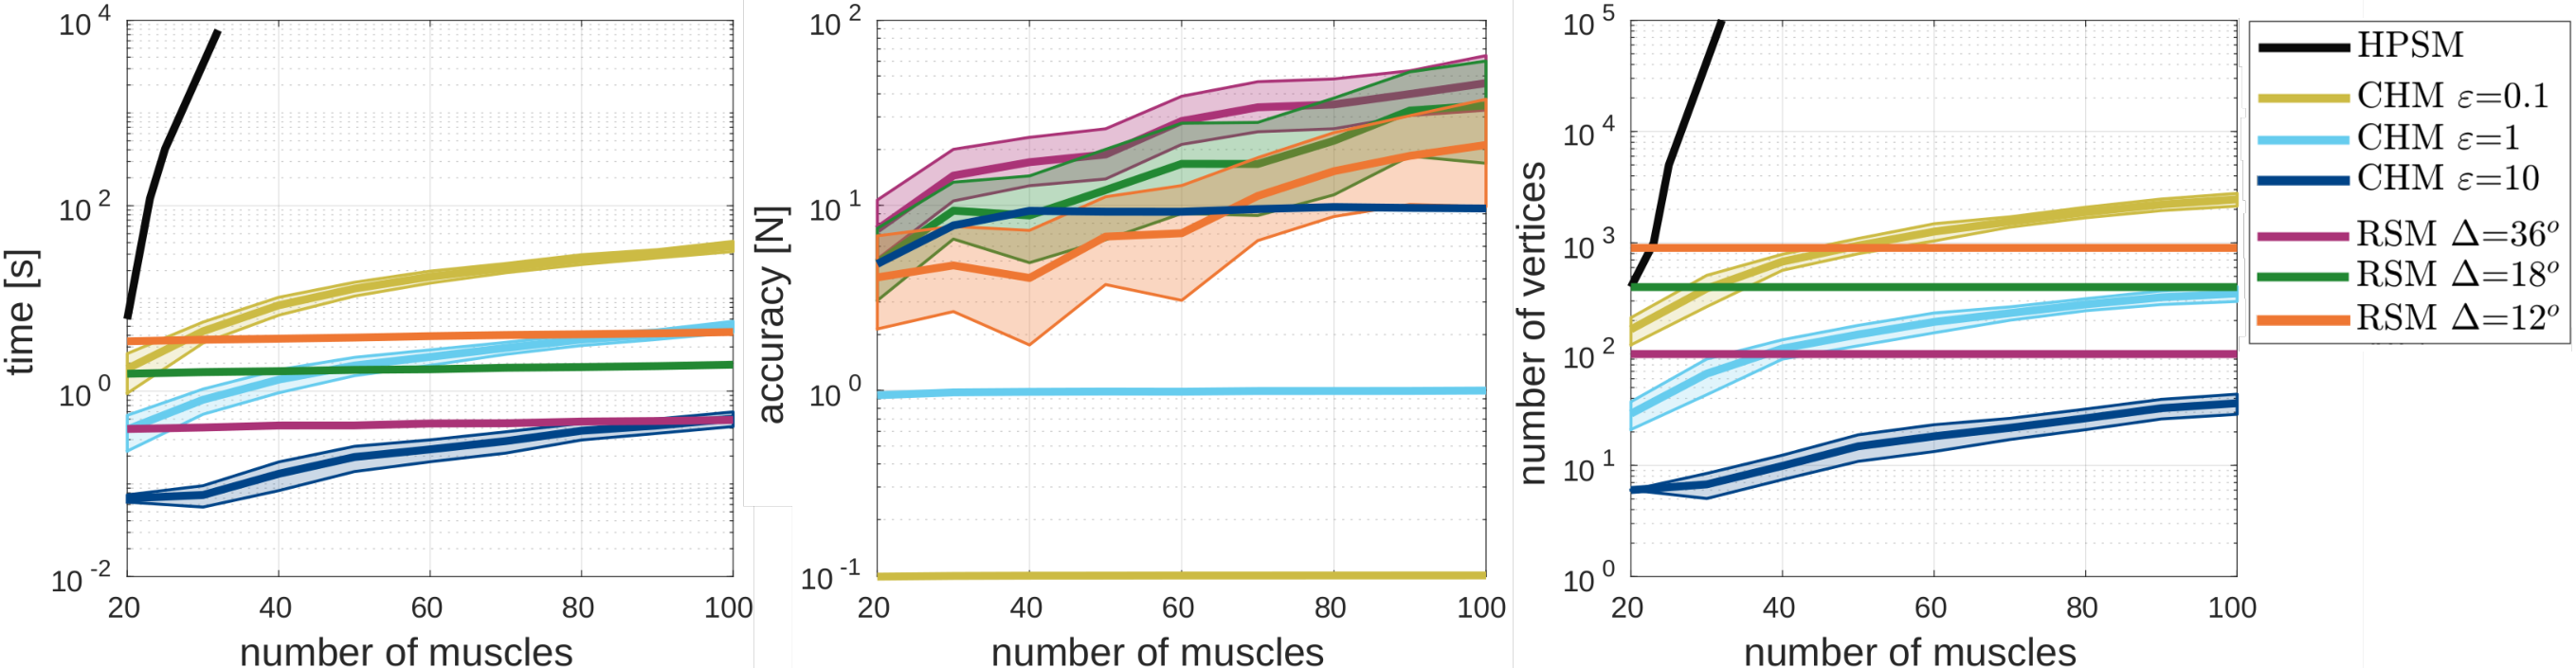
\includegraphics[width=0.95\textwidth]{Papers/images/one_auto_new5}
    \vspace{-0.2cm}
    \caption{\antun{Figure presenting the performance analysis results in the logarithmic scale for three different algorithms: HPSM, RSM and proposed CHM with respect to different number of muscles. Left figure shows the evolution of the execution time. Middle figure shows the evolution of the underestimation error, the maximal distance in between the polytope $\mathcal{P}_x$ and the acquired polytope, calculated as max$\{|\delta_{i}|\}$. Right figure shows the evolution of the number of vertices found. All the plots show the averaged results, with variances, over 100 runs, where each run corresponds to one randomly generated model.}}
    \label{fig:performance_results}
    \vspace{-0.5cm}
\end{figure*}

\section{Performance analysis}

To evaluate the performance of the proposed CHM algorithm, a comparative experiment is performed. The experiment consists in finding the $\mathcal{V}$-rep of the cartesian force $m=3$ polytope for a randomised mockup musculoskeletal model with $n\!=\!7$ degrees of freedom and a number of muscles ranging from $d$ = $20$ to $100$. 

Apart form the proposed method, two additional algorithms are tested. The first algorithm presents an exact approach. It combines the \textit{Hyper plane shifting method} (HPSM) \cite{hyper_psm}, to evaluate the $\mathcal{H}$-rep of the polytope $\mathcal{P}_\tau$, and the \textit{primal-dual} method introduced by Bremer et al. \cite{bremner_fukuda_marzetta_1998}, to find the $\mathcal{V}$-rep of $\mathcal{P}_f$. The second method is the RSM algorithm introduced by Carmichael et al. \cite{carmichael2011Towards} as an example of approximative algorithm used in the context of musculoskeletal models.

The RSM algorithm \cite{carmichael2011Towards} requires uniform sampling of the \textit{ray directions} in the 3D space. This sampling can be performed based on a two Euler angles parametrization. \antun{For this method, three linearly increasing levels of granularity are tested for each Euler angle: $\Delta\!=\!36^o$, $18^o$ and $12^o$;  making for $n_r\!=\!10,20$ and $30$ \textit{rays} per angle. Overall number of \textit{ray directions} in 3D space ($N_r\!=\!n_r^2$) is then $100$, $400$ and $900$. For the proposed CHM algorithm, three exponentially increasing levels of accuracy are tested $\varepsilon\!=\!0.1$, $1$ and $10$ N.} All the algorithms are implemented in Matlab and run on a 1.90GHz Intel i7-8650U processor.

Results of the experiments, averaged over 100 algorithm runs, are shown on figure \ref{fig:performance_results}. The results confirm that the exact approach using the HPSM method has an execution time exponentially related to the number of muscles. Even for only 30 muscles it already takes more than 4.5 h to calculate, therefore this method is not tested on more than 30 muscles, where it finds over $10^4$ vertices.  

The RSM algorithm shows nearly constant time of execution for the full range of tested muscles and the constant number of vertices found, which is expected. The results show however, that for low muscle numbers $d\!<$25, when using a fine granularity $\Delta$=$12^o$ the RSM algorithm finds more vertices than the exact solution found by the HPSM. Furthermore, the middle plot of figure \ref{fig:performance_results} shows that the RSM estimation error increases considerably with the number of muscles $d$, followed by a very
high variance. These results confirm that, as the polytope shape is not spherical, by uniformly covering the space of ray directions, RSM based algorithms will necessarily estimate certain areas of the polytope better than the others.

The graphs show that the proposed CHM method's execution time depends near-linearly of the number of muscles considered $d$ and the estimation error bound parameter $\varepsilon$. The accuracy graph, shown in the middle plot, shows that the proposed CHM algorithm is capable of limiting the estimation error of the polytope evaluation under desired value $\varepsilon$ regardless of the number of muscles. Furthermore, considering the vertex number found by the algorithms, it can be seen that the number of vertices has a nearly-linear relationship with the number of muscles $d$ and the variable $\varepsilon$. 

The demonstrated efficiency of the proposed CHM algorithm opens many doors for its applications in real-time systems, providing the user with an easy to understand trade-off between speed and accuracy.

\antun{
\section{Prospective for human-robot collaboration}
The proposed algorithm presents a new and efficient way of calculating human's wrench capabilities which, as opposed to the known methods (ellipsoids \cite{yoshikawa1985manipulability}\cite{sasaki2011vertex} or RSM algorithm \cite{carmichael2011Towards}), can guarantee user defined level of accuracy. It opens many possibilities for wider use of human wrench polytopes in the area of the human-robot collaboration, by both reducing the computation time and enabling the use of more complete human models, better describing human subjects \cite{sohn2019effects}.

Analysis based on the more complete human models and their pathology could enhance the exoskeleton and prosthesis design, while the efficiency might accelerate analysis of wider anthropomorphic groups of people and improve the design of collaborative workspaces. The algorithm's real-time ability, on the other hand, may enable higher degree of human-centered robot control. The operators' accurate real-time capacity, based on the detailed musculoskeletal models, could be used not only to enforce safety and improve engagement, but to provide the operator-specific assistance profiles. Preventing the development of the work related injuries and potentially even enabling the rehabilitation in the factory context.

% Furthermore, the  also relate to the inclusion of capability alteration models related to fatigue but also cognitive factors. This potential increase in models complexity advocates for systematic experimental validations of the results they lead to \cite{biomechanics1010008}.
}
\section{Conclusion}

\antun{This paper introduces a new generic iterative convex hull based algorithm for evaluating the polytope associated to the class of over-determined problems $A\bm{x}\!=\!B\bm{y}$, where $\bm{y}$ is a set.} The efficiency of the method is demonstrated on the evaluation of the feasible wrench polytope of human musculoskeletal models. In that context, the execution time of the proposed method is shown to be nearly-linear with respect to the number of muscles in the model as well as to the user defined accuracy. 

The potential of the method to be used for collaborative robot control is demonstrated in a collaborative carrying experiment, where the human operator and a robot jointly carry a 7kg object. The experiment shows that by combining the real-time human's capacity evaluation with a simple control law, a highly flexible collaboration scenario can be created. 

\antun{
Even though the proposed algorithm itself is independent of any musculoskeletal model, it relies entirely on the model's real-time representation of the operator. Therefore, for practical implementations, the key challenges become: evaluating human posture in the real-time, precise enough and in a minimally intrusive way, as well as performing the individual scaling and calibration of the used musculoskeletal models for a given operator \cite{correa20112782}.

% \part{Polytope applications}
% % Chapter 1

\chapter{Real-time force capacity based collaborative robot control} % Main chapter title

\label{ch:force_capacity} % For referencing the chapter elsewhere, use \ref{Chapter1} 


%----------------------------------------------------------------------------------------

\section{Collaborative carrying experiment - two robots}
\section{Collaborative carrying experiment - human and robot}
% \chapter{Polytope based task space motion control} % Main chapter title

\label{ch:motion_control} % For referencing the chapter elsewhere, use \ref{Chapter1} 


\section{Robot's capacity aware task space motion planning}
\section{Capacity aware Trapezoidal Acceleration Profile trajectory planning }

% \part{Applications}
% % Chapter 1

\chapter{Real-time force capacity based collaborative robot control} % Main chapter title

\label{ch:force_capacity} % For referencing the chapter elsewhere, use \ref{Chapter1} 


%----------------------------------------------------------------------------------------

\section{Collaborative carrying experiment - two robots}
\section{Collaborative carrying experiment - human and robot}

\chapter{Enhancing human-robot physical collaboration with polytopes}
\label{ch:physical_interaction}

\Cref{ch:phisical_ability_metrics} presentes the benefits of polytope representations of physical abilities for robots and humans, based on their musculoskeletal models. Polytopes, in addition to being their accurate representation, can actually be used as a unifying view on their different physical abilities and allow for characterising their common physical abilities, as one system, in the same polytope form. \Cref{ch:transformin_polytopes} then presents some of the most efficient algorithms, proposed in the literature, for transforming different polytope families into the standard forms suitable for different applications, such as visualisation or robot control. Furthermore, in \Cref{ch:transformin_polytopes}, two new efficient algorithms for polytope transformation are proposed: VEPOLI$^2$ (introduced in \Cref{sec:algorithm_vea}) and ICHM ( introduced in \Cref{ch:algorihtm_ichm}). These algorithms significantly reduce the computational complexity of the polytope transformation and enable their use in real-time applications.

The context of this chapter is put within a collaborative workstation~\cite{SIMOES2022workplace,Bejarano2019}, where
the human and the robot work in a close proximity and interact physically to execute different tasks. Collaborative workstations are promising tools for the future of the small-scale manufacturing \cite{Giberti2022Methodology,wang2022futuristic}, such as the mini-satellite fabrication in the context of the LiChiE project.  
The aim of such collaboration is to improve the overall efficiency by combining the abilities of both humans (flexibility, adaptability, expertise, etc.) and robots (repeatability, precision, tirelessness, etc.), while at the same time improving the operator's safety, and overall well-being, when executing different tasks. 
Therefore, this chapter leverages the efficiency of the proposed algorithms and aims to demonstrate the potential of using polytope representation of human's and robot's physical abilities for creating real-time robot control strategies in the context of human-robot physical collaboration.  

One of the main challenges of such collaborative workstations is creating more adaptive control strategies where the robot adapts its behaviour, not just with respect to the requirements of the task and its own abilities, but also to the current abilities of the human operator, as well as his safety. Creating these collaborative strategies requires having a set of tools for characterising the abilities of robots and humans, as well as quantifying different notions of human's well-being and safety. 

This chapter, therefore, aims to demonstrate that polytope representations of different physical abilities of robots and humans, have a great potential to be used in this context. As showed in \Cref{ch:collab_metrics}, polytopes allow expressing different physical abilities of robots and humans, as well as their collaboration as a single system, in the same polytope form. Such  a unified view enables assessing if different tasks better suite the human's or the robot's abilities, or if they better suite their physical collaboration. This lays the foundation for more adapted objective and quantitative task allocation strategies. Furthermore, as both human's and robot's physical abilities are state dependant and can vary significantly during the task execution, this work proposes to use the polytopes for capturing the changes in their abilities in real-time. 

Having accurate information about robot's physical abilities in real-time, enables creating robot control strategies that adapt to the changes and better exploit robot's abilities. On the other hand, having accurate online information about human's physical abilities enables monitoring the operator's capacity to execute a certain task in real-time. This real-time information can be used to quantify the operators' lacking physical abilities to execute certain task, or in other words, quantify how much assistance they need from the robot. Such monitoring and assistance strategies allow ensuring that their abilities are not surpassed during the task execution, having a direct impact on the operator's safety and well-being. 


Therefore, there are three main concepts that this chapter attempts to explore 
\begin{concept}[C\ref{hyp:individual_capacity}] \label{hyp:individual_capacity} Real-time physical ability information enables creating more adapted control strategies that better exploit robot's and human's individual abilities
\end{concept}

\begin{concept}[C\ref{hyp:common_capacity}] \label{hyp:common_capacity} Real-time physical ability information enables creating  collaborative control strategies that better exploit their common abilities when collaborating physically
\end{concept}

\begin{concept}[C\ref{hyp:safety}] \label{hyp:safety} Real-time physical ability information enables creating  more human-centred robot control strategies improving human's safety
\end{concept}

% \begin{itemize}
%     \item \textbf{H1}: Real-time physical ability information enables creating more adapted control strategies that better exploit robot's and human's individual abilities
%     \item \textbf{H2}: Real-time physical ability information enables creating  collaborative control strategies that better exploit their common abilities when collaborating physically
%     \item \textbf{H3}: Real-time physical ability information enables creating  more human-centred robot control strategies improving human's safety
% \end{itemize}

This chapter is structured as follows. \Cref{ch:collaborative_carrying} brings an example of the task of collaborative object carrying within a collaborative workstation, where two collaborative scenarios are proposed. The first scenario, introduced in \Cref{ch:robot_robot_carrying}, consists in two robots collaborating to carry a heavy object while the control strategies of each one of the robots take in consideration both their own and the other robot's physical abilities. The second scenario, proposed in \Cref{ch:human_robot_carrying}, consists in the human operator and the robot collaboratively carrying a heavy object, where the robot's control strategy takes in consideration its own physical abilities and the physical abilities of the operator in the real-time. \Cref{sec:discussion_perspectives_carrying} brings the discussion on the limitations and perspectives of the proposed experiments and the collaborative control approaches.



% \todos{
% Furthermore, an assistive and human-centred robot control strategy that exploits the polytope geometry is described in section after.
% }

\section{Collaborative carrying of a heavy object}
\label{ch:collaborative_carrying}

\begin{figure}[!h]
    \centering
    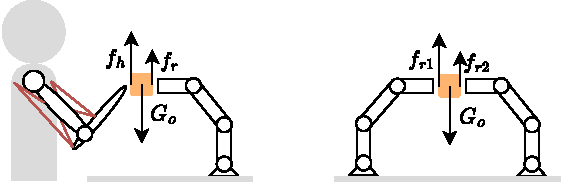
\includegraphics[width=0.8\linewidth]{Papers/images/carrying_schema.pdf}
    \caption{Illustrative example of collaborative object carrying in two different collaborative scenarios, human-robot collaboration on the left and dual robot arm collaboration on the right.}
    \label{fig:carrying_schema}
\end{figure}

One traditional example of a collaborative task requiring physical interaction between multiple actors (humans and robots) is collaborative object carrying~\cite{Arai2000carrying,Kosuge1997carrying,Tsumugiwa2002carrying}. In this task $N$ actors collaborate physically by applying forces $\bm{f}_{a_i}$ on the object with mass $m$, in order to compensate for its gravity $G$
\begin{equation}
    G=m\bm{g}=\bm{f}_{a_1} + ~\cdots ~+\bm{f}_{a_N}
\end{equation}
An illustration of the human-robot and dual robot arm collaborative carrying is given on \Cref{fig:carrying_schema}. As discussed in \Cref{ch:collab_metrics}, in this particular collaboration scenario, each of the actors' capacity to generate forces $\bm{f}_{a_i}$ can be expressed in the polytope form
\begin{equation}
    \bm{f}_{a_i} \in \mathcal{P}_{f,a_i}
\end{equation}
while their joint capacity of generating the forces on the object can be found as the Minkowski sum of their polytopes
\begin{equation}
    \mathcal{P}_f = \mathcal{P}_{f,a_1} \oplus~\cdots~\oplus \mathcal{P}_{f,a_N}
\end{equation}
Therefore if gravity induced force acting the object $G$ is within the polytope $\mathcal{P}_f$ the collaborative system is able to compensate for the objects weight
\begin{equation}
    G \in \mathcal{P}_f
\end{equation}
As both human's and robot's force capacity is state dependant\footnote{The human's and the robot's state force capacity is dependant on their respective states. The exact relationships are described in \Cref{ch:poly_force} for robots and in \Cref{ch:force_poly_human} for humans.} and changes during the execution of the task, the role of the robot control strategies is to find the suitable forces $\bm{f}_{a_i}$ that respect their individual capacities $\mathcal{P}_{f,a_i}$ and accomplish the task by compensating for the object's weight $G$. 

The following two sections present two different robot control strategies for two different collaborative object carrying scenarios. \Cref{ch:robot_robot_carrying} brings a physical collaboration scenario based on two robotic arms carrying an object with a mass of 12kg. Their physical abilities are calculated in real-time in the polytope form and integrated in the real-time robot control in order to exploit their full force capacity. \Cref{ch:human_robot_carrying}, on the other hand, proposes the human-robot physical collaboration scenario for carrying of an object with the mass of 7kg. In this scenario, both of their physical abilities are evaluated online and used to create a human-centred robot control strategy, able to exploit their changing physical abilities while ensuring their safety. 


\section{Dual robotic arm collaborative object carrying}
\label{ch:robot_robot_carrying}

\begin{figure}[!h]
    \centering
    \includegraphics[width=0.9\linewidth]{Papers/images/real_robots_schema_exp1.jpg}
    \caption{Figure showing the experimental setup for dual robot arm collaborative carrying. Two Franka Emika Panda robots jointly carry the object with a mass of $m=12$kg, where each object compensates for a part of the total weight $\bm{f}_{r_1} + \bm{f}_{r_2} = m\bm{g}$. The object is rigidly fixed in the end-effectors of both robots.}
    \label{fig:exp1_real_schema}
\end{figure}


This sections presents a physical collaboration scenario using two {Franka Emika Panda} robots involved in the collaborative carrying on an object of mass $m$. Each robot is contributing to the compensation of the object's gravity $G=m\bm{g}$ by producing forces $\bm{f}_{r_1}$ and $\bm{f}_{r_2}$, such that
\begin{equation}
    \bm{f}_{r_1} + \bm{f}_{r_2} = G
\end{equation}

Panda robots are rated to a maximal carrying capacity of 3kg, which corresponds to the absolute minimal carrying capacity of the robot, evaluated in one of its near-singular configurations. It is, by definition, an underestimation of the real robot's task space force capacity and relying on it, as it is commonly done, limits the scope of the possible tasks and applications.

The goal of this experiment is to demonstrate the fact that by taking into account the true force capacity of each robot, it is possible to go considerably beyond the robot's conservative rated capacity without comprising safety nor exceeding any of the actuation limits\footnote{It it worth noting that the mechanics of the robot's joints might not be designed to withstand the efforts above its rated payload in the long-run. However, this experiment aims to illustrate an optimised use of the robot's abilities, assuming perfectly rigid joints in the directions producing no motion.}. The weight of the object chosen for the experiments is $m=12kg$, voluntarily far above the recommended joint carrying capacity $ m\le 6kg$. 

The following \Cref{sec:robot_carrying_capacity} proposes an efficient approach for calculating the carrying capacity of both robots, leveraging the efficiency of the VEPOLI$^2$ algorithm (described in \Cref{sec:algorithm_vea}). \Cref{sec:collab_robot_control_double_robot} proposes a robot control strategy exploiting this real-time information in order to fully compensate for the continuous evolution of their capacity over time. Finally, \Cref{sec:experiment_dual_robto_carrying} brings the experimental validation of the approach, as well as the discussion of the results. 

\subsection{Robot carrying capacity calculation}
\label{sec:robot_carrying_capacity}


As the carrying task requires the robots to apply only the forces $f_{r_1}$ and $f_{r_2}$ that are opposite to the force of the object's gravity $G$, their physical ability to carry certain weight can be evaluated as the maximal applicable force in the vertical ($z$-axis) direction. Therefore, the robot's carrying capacity $\mathcal{F}_z$ can be expressed as the the special case of the robot's wrench polytope $\mathcal{P}_{f}$, described in \Cref{ch:poly_force}, where the task space is one dimensional ($m=1$)
\begin{equation}
    \mathcal{F}_z (\bm{q},\dot{\bm{q}}) = \mathcal{P}_{f_z} (\bm{q},\dot{\bm{q}}) = \{ f \in \mathbb{R} ~|~ J_{z}(\bm{q})^Tf=\bm{\tau} - \bm{\tau}_b(\bm{q},\dot{\bm{q}}), \quad \bm{\tau}\in[\bm{\tau}_{min}, ~\bm{\tau}_{max}]\}
\end{equation}
where $\{\bm{q},\dot{\bm{q}}\}$ is the robot's joint state, $f \in\mathbb{R}$ is the applicable scalar force in $z$-axis direction, $\bm{\tau}\in\mathbb{R}^n$ are the applied joint torques limited within the interval $\bm{\tau}\in[\bm{\tau}_{min}, ~\bm{\tau}_{max}]$, $\bm{\tau}_{b}\in\mathbb{R}^n$ are the bias joint torques grouping the effects of gravity and robot's motions, while $J_{z}\in\mathbb{R}^{1\times n}$ is the configuration dependant Jacobian matrix with one line and $n$ columns.

\begin{wrapfigure}[14]{r}{0.35\linewidth}
\vspace{-0.5cm}
    \centering
    \includegraphics[width=\linewidth]{Papers/images/carrying_capacity_robot.pdf}
    \caption{A geometric view of constructing the carrying capacity $\mathcal{F}_z$ as the intersection of the force polytope $\mathcal{P}_f$ and the $z$-axis. The carrying capacity is expressed at the center of the object.}
    \label{fig:carrying_cap_robot}
\end{wrapfigure}

Geometrically, the $m=1$ dimensional polytope, describing the range of scalar forces $f$ applicable in the vertical direction, can be represented as the intersection of the complete wrench/force ($m=6$/$m=3$) polytope $\mathcal{P}_f$, described in \Cref{ch:poly_force}, with the vertical axis. An illustrative view of this intersection is shown on \Cref{fig:carrying_cap_robot}.

For any given robot state $\{\bm{q},\dot{\bm{q}}\}$ this one dimensional set $\mathcal{F}_z$ can be transformed into the form of a min-max interval
\begin{equation}
    \mathcal{F}_z = \{ f \in \mathbb{R} ~|~ f \in[{f}_{min}, ~{f}_{max}]\}
\end{equation}
Finding the limits $[f_{min},~f_{max}]$ of the applicable scalar force $f$ in the vertical direction can be viewed as finding a $\repr{V}$-representation of the 1D ($m=1$) polytope $\mathcal{F}_z$. Then the vertex search algorithm VEPOLI$^2$, described in \Cref{sec:algorithm_vea}, can be used to efficiently find the limits (vertices) $f_{min}$ and $f_{max}$ of the applicable force in $z$-axis direction.  

Furthermore, this procedure can be done for both robots $r_1$ and $r_2$, by characterising their carrying capacities
 $\mathcal{F}_{z,r_1}$ and $\mathcal{F}_{z,r_2}$ and finding their applicable vertical force ranges 
\begin{equation}
    f_{r_1} \in [f_{r_1,min}, ~f_{r_1,max} ], \quad f_{r_2}\in [f_{r_2,min}, ~f_{r_2,max}]
    \label{eq:robot_robot_carrying_capacity}
\end{equation}
 
Additionally, their combined carrying capacity $\mathcal{F}_{z,r_1+r_2}$ can be calculated as the Minkowski sum of their polytopes $\mathcal{F}_{z,r_1}$ and $\mathcal{F}_{z,r_2}$ 
$$\mathcal{F}_{z,r_1+r_2} = \mathcal{F}_{z,r_1}\oplus \mathcal{F}_{z,r_2}$$
or in this special case ($m=1$), the sum of their intervals 
$$f_{r_1+r_2} = f_{r_1}+f_{r_2} \in  [f_{r_1,min} + f_{r_2,min}, ~f_{r_1,max} + f_{r_2,max}].$$

In the context of this experiment, the real-time carrying capacity calculation is implemented using the Python open-source library \codet{pycapacity}, developed in the context of this thesis and described in \Cref{ch:software}.

\subsection{Collaborative robot control strategy}
\label{sec:collab_robot_control_double_robot}
The collaborative carrying task requires the robot's to apply forces that compensate for the object's weight $G$, which can be expressed in a form
\begin{equation}
    f_{r_1} + f_{r_2} - G = 0
    \label{eq:robot_robot_weight_compensation}
\end{equation}

In the general case, there exists an infinity of ways the weight can be distributed between the two robots, satisfying equation (\ref{eq:robot_robot_weight_compensation}) and, at the same time, respecting their carrying capacities $\mathcal{F}_{z,r_1}$ and $\mathcal{F}_{z,r_2}$.

In this work, a simple weight distribution strategy is proposed, where the relative load of each of the robots, with respect to their carrying capacity is evenly distributed. 
\begin{equation}
\frac{f_{r_1}}{f_{r_1,max}} = \frac{f_{r_2}}{f_{r_2,max}}
\label{eq:ratio_robot_constant}
\end{equation}
In other words, the weight the robot carries is proportional to its carrying capacity. Combining equations (\ref{eq:robot_robot_weight_compensation}) and (\ref{eq:ratio_robot_constant}), the weight carried by each one of the robots can be expressed as
\begin{equation}
f_{r_1} = \underbrace{\frac{f_{r_1,max}}{f_{r_1,max} + f_{r_2,max}}}_{\lambda_1} G, \qquad f_{r_2} = \underbrace{\frac{f_{r_2,max}}{f_{r_1,max} + f_{r_2,max}}}_{\lambda_2}G 
\label{eq:robot_robot_weight_distribution}
\end{equation}
where $\lambda_1$ and $\lambda_2$ represent the ratios of both robot's contribution to the overall carrying capacity, and their relationship can be expressed as $\lambda_1 + \lambda_2 = 1$.

In order to find the optimal forces $f_{r_1}$ and $f_{r_2}$ that, at the same time, compensate for the weight of the object (\ref{eq:robot_robot_weight_compensation}), comply with the proposed weight distribution strategy (\ref{eq:robot_robot_weight_distribution}) and respect their carrying capacities (\ref{eq:robot_robot_carrying_capacity}), a \gls{qp} based robot control strategy is proposed
\begin{equation}
\begin{split}
    f_{r_1}, f_{r_2} = \underset{f_{r_1},f_{r_2}}{\arg\min} &~\overbrace{||G - f_{r_1} -f_{r_2}||^2}^{\text{weight compensation}} ~~+ \overbrace{ \omega\lambda_2||f_{r_1}||^2 + \omega\lambda_1||f_{r_2}||^2}^{\text{weight distribution}}\\
    s.t.& \quad f_{r_1} \in[f_{r_1,min}, f_{r_1,max}]\\
    & \quad f_{r_2} \in[f_{r_1,min}, f_{r_2,max}]\\
\end{split}
\label{eq:qp_robot_robot}
\end{equation}

The proposed optimisation problem consists in two tasks. The first task is the weight compensation task, corresponding to equation (\ref{eq:robot_robot_weight_compensation}), which is ensured by minimising the error $||G - f_{r_1} -f_{r_2}||^2$. Expressing equation (\ref{eq:robot_robot_weight_compensation}) in this form, allows for the cases when the robot's carrying capacities are not sufficient for carrying the object $f_{r_1,max} + f_{r_2,max}<G$. Preventing such situations and ensuring the feasibility of the robots' tasks presents a substantial research challenge in the realm of robot task design. 

In the context of collaborative carrying task, a potential avenue in addressing this issue comes from wrench feasibility analysis \cite{gouttefarde2006determination,Lau2011}. These tools could enable quantifying the areas of the collaborative workspace, where a certain weight compensation capacity is guaranteed. Then, the collaborative carrying tasks could be designed within these ares in the workspace. It's worth noting that these approaches complement the proposed approach and could be used in tandem to further improve the robustness of the proposed method and bring it a step closer to practical real-world applications.  

\begin{figure}[!b]
    \centering
    \includegraphics[width=\linewidth]{Papers/images/schema_robot_robot.pdf}
    \caption{The block diagram showing the implemented robot control scheme. Each robot's low-level force control loop runs at 1kHz, while the carrying capacity calculation and the collaborative control strategy are evaluated at the frequency of 100Hz.}
    \label{fig:schema_robot_robot_control}
\end{figure}


The second task ensures the even relative load distribution between the robots, as proposed by the weight distribution strategy given in equation (\ref{eq:robot_robot_weight_distribution}). To achieve this behaviour, the norm of the first robot's force $f_{r_1}$ is weighted by the second robot's contribution ratio $\lambda_2$, while the second robot's force $f_{r_2}$ is weighted by the first robot's contribution ratio $\lambda_1$. This way, if the robot $r_1$ has higher carrying capacity $f_{r_1,max}>f_{r_2,max}$, the force $f_{r_1}$ is weighted (penalised) less in the cost function $\lambda_1>\lambda_2$, ultimately resulting in higher values found by the optimisation problem for robot 1. On the other hand, if the carrying capacities of both robots is equal, then the weighing factors are equal too $\lambda_1=\lambda_2$, resulting in the equal weight distribution. 

The factor $\omega$ is used to set the priority of the weight distribution task much lower than the main task of the weight compensation of the object, in the experiments proposed in this sections the regularisation weight is set to $\omega=1\times 10^{-5}$.

Each robot control cycle starts by calculating the carrying capacities (\ref{eq:robot_robot_carrying_capacity}), followed by the resolution of the optimisation problem (\ref{eq:qp_robot_robot}). Once the optimal vertical forces $f_{r_i}$, are obtained the joint torques $\bm{\tau}_{r_i}$, achieving those forces, are calculated for each of the robots and sent to their low-level joint controllers 
\begin{equation}
    \bm{\tau}_{r_i} = J_{z,r_i}^T(\bm{q}_{r_i}){f}_{r_i} + \bm{\tau}_{b,r_i}(\bm{q}_{r_i},\dot{\bm{q}}_{r_i}), \qquad \forall i \in \{1,2\}
\end{equation}

The calculation of the carrying capacity of both robots and the proposed collaborative control strategy are implemented in programming language Python and performed at the frequency of 100Hz.  The robot's open-loop force control is implemented in programming language C++, using the library \codet{pinocchio}~\cite{pinocchio2021}, and run at the frequency of 1kHz. The complete software stack has been integrated using the \gls{ros}~\cite{ros} programming environment and run from one computer equipped with a 1.90GHz Intel i7-8650U processor. 
\Cref{fig:schema_robot_robot_control} shows the schematic block diagram of the implemented collaborative robot control strategy. 

\subsection{Experimental validation}
\label{sec:experiment_dual_robto_carrying}
\begin{figure}[!h]
    \centering
    \includegraphics[width=\linewidth]{Papers/images/exp1_explication.jpg}
    \caption{This figure shows the experimental setup and visualises the trajectory taken by the human operator. The robots compensate for the full object's weight while the operator moves the object through the workspace, doing a forward and backward pass through the 4 via-points.}
    \label{fig:experiment1}
\end{figure}

\qrimg{qrcodes/icra2021.png}{https://youtu.be/hApIv1oFuhk}{Video}
In this experiment the two Panda robots jointly compensate for the weight of the object (12 kg), using the proposed collaborative control strategy. A human operator freely moves the object through the common work-space, implicitly changing both robots' configurations in real-time. As a consequence, the task space trajectory and the evolution of the robot configurations are not known in advance. 

The particular trajectory taken by the human operator in this experiment is indicated on \Cref{fig:experiment1}. It consists in taking the object through the set of four via-points, making a forward and backward pass. The proposed control strategy then leverages the real-time calculation of their carrying capacity and adapts the weight distribution to ensure the compensation of the full object's weight during the whole experiment. 

\afterpage{
\begin{landscape}
\begin{figure}
    \centering
    \includegraphics[width=\linewidth]{Papers/images/exp_no_anim.jpg}
    \caption{This figure shows the time evolution of different control and physical ability variables in the top graphs, as well as several images of the experiment taken when the operator attained different via-points with the object. 
   The top graph shows the time evolution of the carrying capacity of the manipulators $f_{r_1,max},f_{r_2,max}$, indicating, with red background, the time periods when the naive strategy $f_{r_1}=f_{r_2}=0.5G$ (dashed line on all graphs) would not be feasible for at least one of the two robot. 
   The second  graph provides the evolution of their joint capacity $f_{max}=f_{r_1,max}+f_{r_2,max}$, indicating their individual contributions to the common capacity. The third graph indicates the time evolution of applied manipulator forces $f_{r_1}, f_{r_2}$, calculated using the proposed control strategy. Finally, the bottom graph shows the time evolution the weights $\lambda_1,\lambda_2$ used with the robot control. All the force values are expressed in kilograms for easier readability.     
    }
    \label{fig:dual_manip}
\end{figure}
\end{landscape}
}

A straightforward control strategy, requiring each robot to compensate for half of object mass $f_{r_1}=f_{r_1}=0.5G$ is taken as baseline to evaluate the performance of the new method. This experiment is illustrated in the accompanying video\footnote{Video: \url{https://youtu.be/hApIv1oFuhk}}.

\Cref{fig:dual_manip} (bottom) shows several images taken during the experiment execution, in the moments when the operator reached different via-points. The graphs on the top show the time evolution of the evaluated maximal forces and force applied by each robot during the experiment. The naive strategy $f_{r_1}=f_{r_1}=0.5G$ is shown in dashed lines for comparison. 


The results show that the proposed control strategy is successful in ensuring compensation of the object weight during the full length of the experiment. In the starting via-point $t=0$s and $t\geq21$s, robot $r_2$ (robot on the right) is close to it's singular configuration and its load carrying capacity is close to $5$kg. Controlling it to compensate for half of the weight of the object would result in a saturation of the actuators and potential damage to the hardware. The same is true for via-point 4 at $t=12$s. In this via-point the robot $r_1$ (robot on the left) is not be able to compensate for half of the object weight, but thanks to the proposed adaptive control law, the task can successfully be achieved, supporting \Myref{hyp:individual_capacity}. 
Furthermore, any naive fixed strategy, assigning certain fixed ratio of the object's weight to the robots, would result in surpassing the robots' limits which in turn would fail to accomplishing the task. 
By exploiting the online calculation of the robots' physical abilities, the proposed strategy enables exploiting their changing abilities and accomplishing this task while at the same time guaranteeing that their capacities are not exceeded. 

The results further show that even though in the large portion of the experiment one of the robots was not able to carry half of the object's weight, their joint carrying capacity exceeded the objects weight $f_{r_1,max}+f_{r_2,max} >G$ during the whole length of the experiment, conforming with \Myref{hyp:common_capacity}.

However, this may not be the case over the entire common workspace of the two robots, but this example is a good illustration of the interest of accounting for the true capabilities of the system at the control level.  In certain configurations the common carrying capacity of the robots might be lower than the objects weight $f_{r_1,max}+f_{r_2,max} <G$. The proposed control approach, in those cases would ensure that the robots' physical abilities are not exceeded, however it would not be able to guarantee the weight compensation of the object. 

In summary, the experimental validation demonstrates the effectiveness of the proposed control strategy in real-time adaptation of weight distribution between multiple robots based on their varying physical abilities. The strategy ensures safe and efficient collaboration between robots, allowing them to collectively perform tasks that would be challenging or impossible for each robot to accomplish individually. Leveraging real-time information about their physical abilities, the proposed strategy offers a flexible solution for collaborative applications, eliminating the need for pre-calibration or in advance task-specific information.

\section{Human-robot collaborative object carrying}
\label{ch:human_robot_carrying}

\begin{figure}[!h]
    \centering
    \includegraphics[width=0.9\linewidth]{Papers/images/exp2_real_schema.jpg}
    \caption{This figure show the experimental setup. The robot end-effector is fixed to the carried object and the human operator is holding the object by the handle. The object's mass is $m=7$kg, while the operator and the robot collaborate to compensate the full weight of the object.}
    \label{fig:exp2_real_schema}
\end{figure}

In many industrial contexts, including the LiChiE project's mini-satellite fabrication process, tasks involving the manipulation of heavy objects are a frequent occurrence. 
Taking inspiration from these tasks, this section presents an illustrative scenario where a human and a robot collaborate physically to carry a heavy object. In this scenario, shown on \Cref{fig:exp2_real_schema}, a human operator and a {Franka Emika Panda} robot jointly carry an object mass of $m\!=\!7$ kg, each one compensating for a part of the total weight 
\begin{equation}
    \bm{f}_h  + \bm{f}_r = m\bm{g} = G
\end{equation}

In this experiment, the operator has the expert knowledge about the task and moves the object through the workspace to perform the task efficiently. The robot's role, in this case, is to assist the operator with the carrying of the heavy object and improve their safety and their overall well-being.

The usual choice for these scenarios is a simple gravity compensation strategy, making the robot carry the full weight of the object $\bm{f}_r = G$ and provide the operator with full movement transparency. Several such human-centred robot control strategies have recently been proposed in the literature, where the robot in addition to the full weight compensation improves different aspects of the human safety and ergonomics. One example of such approach is proposed by \citet{ferraguti2020unified}, which REBA \cite{reba} ergonomic indicators to improve human posture while carrying an object. 

However, as discussed in \Cref{ch:robot_robot_carrying}, assigning any fixed weight to the robotic manipulator requires \textit{a priori} analysis of its changing capacity and determination of the \textit{worst-case} weight limits, which in the case of the Franka Emika Panda robot is $m\leq3$kg\footnote{Given by the manufacturer in the form of the robot's rated payload.}. Therefore, carrying the 7kg load requires using a more capable robot which, in many cases, significantly increase the cost of such system and potentially reduces operator's safety. As more capable robots are usually bigger and heavier, they result in much higher exchanged forces in case of impact with the operator, raising many safety concerns~\cite{smu}.
Therefore, delegating the entire weight compensation to the robot is not always the most efficient or the safest solution for the operator. 

On the other hand, several studies have shown that the human's physical feedback during task execution improves significantly their engagement in the task \cite{rani2007operator}, improves the task execution efficiency and reduces the risk of error \cite{BYRNE1996249}. However, since the human's carrying capacity varies significantly throughout the workspace as well, before allocating any weight to the operator, their safety has to be ensured. As in the case of robots, the traditional approach consists in analysing the task in advance and determining, often in a very conservative manner, the set of \textit{worst-case} limits \cite{shoaf1997comprehensive}, often given in a form of different standards \cite{nasa} and manuals \cite{health1992manual}. 

In order to avoid making such coarse assumptions, several approaches have been proposed in the literature, able to quantify different measures of human physical abilities and adapt the human load to their changes online. \citet{Kim2018} have proposed an approach estimating the joint torques in the operator's body produced by carrying the load of the object, where the robot's role is to adapt the operator's posture to minimise the magnitude of human's joint torques. The human body is approximated using a planar model actuated at the joint level. Furthremore, in their work, the human is the one carrying the full mass of the object, while the robot's only role of is to modify the operator's posture in order to improve his ergonomics. 

A different approach is proposed by \citet{carmichael2013admittance}, where the human and the robot collaborate physically to execute the carrying task. Their approach is employs on a more accurate human model, based on human musculoskeletal models, which is used to efficiently approximate the human's force capacity. The robot control strategy modulates the weight carried by the human with respect to the approximation calculated in real-time. The approach is developed in the context of human rehabilitation and used for the real-time control of assistive exoskeletons. The authors show that such approach is capable of adapting to the operator's pathology and reduce the rehabilitation time~\cite{Carmichael2013Experimental}. 
This approach demonstrates the potential of using human-centred robot control strategies which are able to adapt the load carried by the human precisely to his varying physical abilities. However due to the intractable computational complexity of the human force capacity calculation proposed by the authors, the scope of their work is limited to relatively simple planar musculoskeletal models. Furthermore, the robot control strategy proposed in their work is aimed to the rehabilitation and the use of assistive exoskeletons, which does not transpose well to more unstructured industrial scenarios.

Inspired by their work, this section aims to further demonstrate the potential of using the real-time knowledge about both robot's and human's physical abilities in the context of collaborative robot control in industrial scenarios. The proposed collaborative robot control strategy leverages the two new algorithms developed in the context of this work, capable of efficiently calculating the force capacity of robots (VEPOLI$^2$ described in \Cref{sec:algorithm_vea}) and humans, based on their musculoskeletal models (ICHM described in \Cref{ch:algorihtm_ichm}). 
Their changing capacities are calculated online and used to create collaborative robot control strategy, capable of both exploiting their full potential and, at the same time, ensure the safety of the operator. 

\Cref{sec:human_carrying_capacity} introduces an efficient strategy for calculating the operator's carrying capacity in real-time. \Cref{sec:collab_robot_control_human_robot} introduces the collaborative robot control strategy using the online information about the operator's carrying capacity, as well as the robot's capacity, described in  \Cref{sec:robot_carrying_capacity}. The experimental validation of this approach is described in  \Cref{sec:human_robot_experiment} as well as the discussion on results.

\subsection{Human carrying capacity calculation}
\label{sec:human_carrying_capacity}

As described in \Cref{ch:human_metrics}, the analysis of human's physical abilities in this work is based on their musculoskeleral models, as the most accurate models of human bodies currently available.
More specifically, as shown on \Cref{fig:exp2_real_schema}, this experiment requires evaluating the operator's ability to carry the object in his right arm. 
Many different human arm musculoskeletal models are proposed and validated in the biomechanics literature \cite{holzbaur2005model,saul2015benchmarking}, as well as different software tools for their analysis \cite{opensim,Bouchard2009}. 
However, choosing an appropriate musculoskeletal, and adapting it to individual characteristics of the operator, is a challenging scientific problem. 

In broad terms, using more detailed musculoskeletal models often leads to more accurate representation of human subjects \cite{sohn2019effects}, but comes with an increase in the computational complexity. 
The computational efficiency of the proposed ICHM algorithm, described in \Cref{ch:algorihtm_ichm}, allows for considering relatively detailed models (even up to 50 muscles) while maintaining interactive execution times. 
Therefore, the analysis in this section assumes having an appropriate and detailed musculoskeletal model of the operator's arm. 

When it comes to the collaborative carrying experiment, the operator is required to apply only the force $f_{h}$ that contributes to compensating the object's gravity $G$. Therefore, the task is effectively one dimensional $m=1$ and his physical ability to carry certain weight can be evaluated as the maximal applicable force in the vertical ($z$-axis) direction. Hence, the human's carrying capacity $\mathcal{F}_z$ can be expressed as the the special case of the human's wrench polytope $\mathcal{P}_{f}$, described in  \Cref{ch:force_poly_human}, where the task space is one dimensional ($m=1$)
\begin{equation}
     \mathcal{F}_z(\bm{q},\dot{\bm{q}}) = \mathcal{P}_{f_z} (\bm{q},\dot{\bm{q}}) = \{ f \in \mathbb{R} ~|~ J_{z}(\bm{q})^Tf=N(\bm{q})\bm{F} - \bm{\tau}_b(\bm{q},\dot{\bm{q}}), \quad \bm{F}\in[\bm{F}_{min}, ~\bm{F}_{max}]\}
\end{equation}
where $\{\bm{q},\dot{\bm{q}}\}$ represent the human's joint state, $f \in\mathbb{R}$ is the applicable scalar force in $z$-axis direction, $\bm{F}\in\mathbb{R}^n$ are the applied muscular forces limited within the interval $\bm{F}\in[\bm{F}_{min}, ~\bm{F}_{max}]$, $\bm{\tau}_{b}\in\mathbb{R}^n$ represents the bias joint torques grouping the effects of the gravity and human's motions, while $J_{z}\in\mathbb{R}^{1\times n}$ is the configuration dependant Jacobian matrix with one line and $n$ columns and $N\in\mathbb{R}^{n\times d}$ is the state dependant moment arm matrix. Values $n$ and $d$ correspond to the number of joints and muscles considered in the musculoskeleral model.

Analogously to the robot's case, human's carrying capacity $\mathcal{F}_z$ is a $m=1$ dimensional polytope, describing the range of scalar forces $f$ applicable in the vertical direction. Geometrically, this polytope corresponds to the intersection of the complete wrench/force ($m=6$/$m=3$) polytope $\mathcal{P}_f$, described in \Cref{ch:force_poly_human}, with the vertical axis. An illustrative view of this intersection is shown on \Cref{fig:carrying_cap_human}.

Furthermore, for any given human's state $\{\bm{q},\dot{\bm{q}}\}$ this one dimensional set $\mathcal{F}_z$ can be transformed into the form of a min-max interval
\begin{equation}
    \mathcal{F}_z = \{ f \in \mathbb{R} ~|~ f \in[{f}_{min}, ~{f}_{max}]\}
\end{equation}
In order to find the limits $[f_{min},~f_{max}]$ of the applicable scalar force $f$ in the vertical direction, this problem can be formulated as finding the $\repr{V}$-representation of the 1D ($m=1$) polytope $\mathcal{F}_z$. Then the real-time capable algorithm ICHM, proposed in \Cref{ch:algorihtm_ichm}, can then be used to find the limits (vertices) $f_{min}$ and $f_{max}$ of the applicable force in $z$-axis direction.  


\begin{wrapfigure}{r}{0.4\linewidth}
    \centering
    \includegraphics[width=\linewidth]{Papers/images/carrying_capacity_human.pdf}
    \caption{A geometric view of constructing the carrying capacity $\mathcal{F}_z$ as the intersection of the force polytope $\mathcal{P}_f$ and the $z$-axis. The carrying capacity is expressed at the center of the object.}
    \label{fig:carrying_cap_human}
\end{wrapfigure}
Following the similar procedure as for humans, the robot's carrying capacity can be determined in real-time as well, using the VEPOLI$^2$ algorithm, as proposed in \Cref{sec:robot_carrying_capacity}. Then the human's carrying capacity $\mathcal{F}_{z,h}$ and robot's carrying capacity $\mathcal{F}_{z,r}$, characterising their feasible ranges of applicable vertical forces $f_r$ and $f_h$ can be expressed as in the form of ranges
\begin{equation}
    f_{h}\in [f_{h,min}, ~f_{h,max}], \qquad f_{r} \in [f_{r,min}, ~f_{r,max} ]
    \label{eq:human_robot_carrying_capacity}
\end{equation}

Additionally, their combined carrying capacity $\mathcal{F}_{z,h+r}$ can be calculated as the Minkowski sum of their carrying capacities $\mathcal{F}_{z,h}$ and $\mathcal{F}_{z,r}$ 
$$\mathcal{F}_{z,h+r} = \mathcal{F}_{z,h}\oplus \mathcal{F}_{z,r}$$
or in this special ($m=1$), the sum of the intervals 
$$f_{h+r} = f_{h}+f_{r} \in  [f_{h,min} + f_{r,min}, ~f_{h,max} + f_{r,max}].$$

As in the previous experiment, the real-time carrying capacity calculation, using VEPOLI$^2$ and ICHM algorithms, is implemented using the Python open-source library \codet{pycapacity}. This library is developed in the context of this thesis in \Cref{ch:software}.

\subsection{Collaborative robot control strategy}
\label{sec:collab_robot_control_human_robot}

The collaborative carrying task requires the human and the robot to apply forces that combined compensate for the object's weight $G$ 
$$f_{h} + f_{r} = G$$
As their carrying capacity changes in time, the main task of the robot's control algorithm consists in modulating the weight carried by the operator and the robot to ensure that their carrying capacity is not exceed while compensating for the object's weight.

In addition to the object's weight compensation, inspired by the \gls{aan} paradigm proposed by 
\citet{carmichael2013admittance}, a simple adaptive weight distribution strategy is proposed, with the goal to ensure that the human operator's relative load remains constant with respect to its real-time capacity. 
$$\frac{f_h}{f_{h,max}} = const.$$
The fixed ratio chosen for the experiments is 30\% of the human's carrying capacity, ensuring operator's safety and maintaining the constant level of engagement.  
$$
f_h = 0.3 f_{h,max}
$$ 
It is worth acknowledging that determining the optimal ratio is a challenging scientific problem, one that may require individual determination for each human subject. In the context of this work, the value of 30\% is selected arbitrary.

The main task of the object's weight compensation as well as the \gls{aan} strategy, maintaining the constant relative load of the operator, is implemented in a single robot control strategy based on \gls{qp}
\begin{equation}
\begin{split}
    f_r,f_h =\underset{f_r,f_h}{\arg\min} &~\overbrace{||G- f_r -f_h||^2}^{\text{weight compensation}} ~~+ \overbrace{\omega||f_r||^2}^{\text{weight distribution}}\\
    s.t.& \quad f_h \in[0.3f_{h,min}, ~0.3f_{h,max}]\\
    & \quad f_r \in[f_{r,min}, ~f_{r,max}]\\
\end{split}
\label{eq:qp_human_robot}
\end{equation}
The main component of the cost function of this \gls{qp} is the minimisation of the error~${||G\! -\! f_{h}\! -\!f_{r}||^2}$, which ensures that the object's gravity is always compensated, as long as their carrying capacity defined in the constraints of the optimisation problem allows for it. 

The \gls{aan} strategy is formulated as a regularisation task $\omega||f_r||^2$ in the cost function. This task minimises the magnitude of force $f_{r}$ applied by the robot while having no penalisation for the human's force $f_h$. The resulting behaviour of the optimisation problem is to find the weight distribution between the human and the robot which results in the minimal force $f_{r}$ applied by the robot, while maximising the force of the operator $f_h$. In the other words, this weight distribution strategy produces the \gls{aan} behaviour where the human applies its maximal forces (30\% of its carrying capacity) while the robot compensates for the rest. More precisely, the force the human applies is equal either to 30\% of its carrying capacity or the full objects weight
$$
f_h = \begin{cases}
    0.3f_{h,max},& \text{if } G\geq 0.3f_{h,max}\\
    G,              & \text{otherwise}
\end{cases}
$$
while the robot carries the remaining weight, as long as it is capable of doing so
$$
f_r =  \begin{cases}
    G-f_h,& \text{if } G-f_h\leq f_{r,max}\\
    f_{r,max},              & \text{otherwise}
\end{cases}
$$
It is worth noting that, if the object's weight exceeds the common carrying capacity of the robot and the operator $$f_{r,max} + 0.3f_{h,max} < G$$
they are not able to compensate for the weight. In such scenarios, the proposed strategy will prioritise ensuring that their capacities are not exceeded, over the weight compensation.

The regularisation factor $\omega$ is used to set the priority of the \gls{aan} task lower than the main task of the weight compensation of the object. In the experiments proposed in this section the regularisation weight is set to $\omega=1\times 10^{-2}$.


\begin{figure}[!b]
    \centering
    \includegraphics[width=\linewidth]{Papers/images/schema_human_robot.pdf}
    \caption{Block diagram showing the implemented robot control scheme. The robot's low-level force control loop runs at 1kHz, while the carrying capacity calculation of both robot and the operator, as well as the collaborative control strategy, are evaluated at the frequency of 100Hz. Human's posture is obtained using the motion capture system OptiTrack.}
    \label{fig:schema_human_robot_control}
\end{figure}

In each control cycle human's $\mathcal{F}_{z,h}$ and robot's $\mathcal{F}_{z,r}$ carrying capacities are calculated. These values are then used for the resolution of the optimisation problem (\ref{eq:qp_human_robot}). Once the robot's optimal vertical force $f_{r}$ is obtained, the joint torques $\bm{\tau}_{r}$ achieving this force are calculated using the expression
$$
\bm{\tau}_r = J_{z,r}^T(\bm{q}_r) f_r + \bm{\tau}_{b,r}(\bm{q}_r,\dot{\bm{q}}_r)
$$
where $\{\bm{q}_r,\dot{\bm{q}}_r\}\in \mathbb{R}^{n_r}$ is the robot's $n_r$ dimensional state, $J_r\in\mathbb{R}^{\times n_r}$ is the end-effector Jacobian with 1 line and $n_r$ columns, $\bm{\tau}_{b,r} \in\mathbb{R}^{n_r}$ is robot's torque vector corresponding to the effects of the gravity and the robot's motion and $\bm{\tau}_r \in\mathbb{R}^{n_r}$ are the joint torques sent to the robot's low-level joint control. 

The human's force $f_h$, calculated by the proposed control strategy, corresponds to the force the operator should apply in order for the object to stay static in the space. As the weight compensation is both operator's and robot's task, the operator will naturally tend to apply the force $f_h$. 
Therefore, the proposed control strategy indirectly closes the loop with the human operator through the forces applied on the object.

Both robot's and human's carrying capacity calculation algorithms, as well as the robot control strategy described in \Cref{sec:collab_robot_control_human_robot}, are implemented in Python and run in real-time with the update frequency of 100Hz. The low-level robot control is implemented in C++, using the open-source library \codet{pinocchio}~\cite{pinocchio2021}, and run in real-time at the frequency of 1kHz. All the software components are integrated using the \gls{ros}~\cite{ros} and run on a computer equipped with a 1.90GHz Intel i7-8650U processor. 
\Cref{fig:schema_human_robot_control} shows the schematic block diagram of the implemented collaborative robot control strategy. 

\subsection{Experimental validation}
\label{sec:human_robot_experiment}

\begin{figure}[!h]
    \centering
    \includegraphics[width=\linewidth]{Papers/images/both_pose_explanation.jpg}
    \caption{{These figures show the experimental setup. The robot end-effector is fixed to the carried object and the human operator is holding the object by the handle. The motion capture system is used to acquire the pose of the human arm. The via-points are visually indicated to the human operator with numbered stickers on the table placed at the corners of a 30 cm square. The images shows the experiment 1 (left) and the experiment 2 (rigth).}}
    \label{fig:experiment2}
\end{figure}

\qrimg{qrcodes/icra2022.png}{https://youtu.be/wg4E62AkNnM}{Video}
In this experiment, the human operator performs a task by {visually} navigating the object through the common workspace, passing through {the set of} 4 via-points. The object is fixed in the end-effector of the robot as well as at the hand of the human operator using a handle. \Cref{fig:experiment2} shows the experimental setup indicating the structure of the collaborative workstation, the placement of the via-points and the handle. 

The experiment is repeated two times, for two different operator positions, equally distant from the via-points, but rotated by 90° in space. These operator positions are indicated on \Cref{fig:experiment2} as well. Furthermore, in each of the two experiments, the operator performs 10 cycles through the via-points. The experiment is illustrated in the accompanying video\footnote{Video: \url{https://youtu.be/wg4E62AkNnM}}.



\begin{wrapfigure}{r}{0.4\linewidth}
\vspace{-0.5cm}
    \centering
    \includegraphics[width=\linewidth]{Papers/images/model_50m7dof.png}
    \caption{Human right arm musculoskeletal model MOBL-ARMS \cite{saul2015benchmarking}, with 50 muscles and 7 joints. Visualised using OpenSim software \cite{opensim}.  }
    \label{fig:model_musc}
\end{wrapfigure}
The musculoskeletal model used in this experiment is the MOBL-ARMS model \cite{saul2015benchmarking} of the human upper limb (right arm), developed by \citet{holzbaur2005model}. A relatively detailed model consisting in 50 muscles ($d=50$) and 7 degrees of freedom ($n=7$). The visualisation of this model, using the biomechanics software Opensim \cite{opensim}, is shown on \Cref{fig:model_musc}.
The operator's arm configuration is inferred in real-time using an OptiTrack~\cite{optitrack} motion capture system. The musculoskeletal model is obtained using the efficient biomechanics library \codet{biorbd} \cite{Michaud2021}. 

The human subject (male, 182 cm, 80 kg) and the MOBL-ARMS model belong to the same 50th percentile anthropomorphic group \cite{gordon1989anthropometric} so no model adaptation is necessary (ex. scaling \cite{correa20112782}).

\Cref{fig:experiment_results} shows the recorded time evolution of robot's and human's carrying capacities and weight carried during the 10 cycles for each of the two experiments. 

The figure shows (top graphs) that the human's carrying capacity is much more variable than the robot's one, peaking around 20kg in the recorded experiments and going as low as 5kg, emphasising the importance of measuring it in real-time, and supporting \Myref{hyp:individual_capacity}. Furthermore, the experiment's show that the human's carrying capacity is in many cases much higher than the robot's capacity, confirming the importance of creating the control strategies able to account for both of their physical abilities. 

\afterpage{
\begin{landscape}
\begin{figure}[!t]
    \centering
    \includegraphics[width=\linewidth]{Papers/images/exp2_new.jpg}
    \caption{This figure shows the evolution of the carrying capacity and weight carried by the operator and the robot over the course of the via-point cycle, for two experiments. The plots show mean values and the variances of the curves calculated over 10 successive cycles. The graph regions belonging to the different via-points are separated by vertical lines.  All the values are expressed in kilograms for easier readability.}
    \label{fig:experiment_results}
\end{figure}
\end{landscape}
}

The second line of graphs on \Cref{fig:experiment_results} shows the time evolution of the sum of their carrying capacities, their common carrying capacity as one system. The graphs show that even though both the robot and the human, in multiple instances during the experiment runs, had carrying capacity lower than the object's weight $G$, their joint carrying capacity exceeds the object's weight during the whole time of the experiment. Therefore, the proposed method demonstrates the feasibility of using physical ability aware control strategies to improve the performance of the physical collaboration. This confirms \Myref{hyp:common_capacity} by showing that, even though, neither the operator or the robot would have been able to carry the object on their own, by collaborating, they were able to execute this task.

It is worth noting that the objective of this experiment is to demonstrate the feasibility rather than guarantee universal applicability. In more general situations, there could be scenarios where the collective carrying capacity of the human and the robot is insufficient to support the object's weight ($f_{h,max}+f_{r,max} <G$). In such cases, the introduced control strategy prioritises ensuring that both actors capacities are not exceeded rather than the complete compensation for the object's weight.

The third line of graphs shows the time evolution of the weight carried by the robot and the human, while the bottom graphs on \Cref{fig:experiment_results}, show the relative load of the robot $l_r$ and the human $l_h$ calculated as
$$
l_h = \frac{f_h}{f_{h,max}}, \qquad\qquad l_r = \frac{f_r}{f_{r,max}}
$$

The graphs confirm that the proposed control strategy maintained the human's relative load at 30\% ($l_h=0.3$) of its capacity as proposed by the \gls{aan} strategy, while the robot's relative load $l_r$ depended on the human capacity. As the human's carrying capacity decreased robot's load $l_r$ increased, and \textit{vice-versa}. By having the real-time knowledge about the operator's carrying capacity, the robot was able to adapt its assistance level to maintain human's load constant, despite substantial changes in the operator's capacity profile and despite his changing placement placement with respect to the task, supporting the \Myref{hyp:safety}.

% In summary, the experimental validation, presented in this section, demonstrates the benefits of integrating accurate real-time information about both the human operator's and the robot's physical abilities within the robot control strategy, in the context of human-robot physical collaboration.

% The proposed robot control strategy exploits both robot's and human's physical abilities, while guaranteeing that neither of their abilities is surpassed. As demonstrated in the experiments, even though their individual abilities are not suitable for executing this task on their own, by collaborating the task become feasible, as their combined abilities (as a single system) are higher than the requirements of the task. In addition to efficiently combining both operator's and robot's physical abilities, the proposed control strategy was able to further ensure safety and operator's engagement in the task, by modulating the weight carried by the human operator in accordance with the proposed \gls{aan} strategy. 

% Finally, the proposed strategy relies entirely on the real-time information about the carrying capacities, enabling very flexible collaborative behaviours, where the robot is able to adapt to any trajectory chosen by the operator as well as to the change in his placement in space. 

\section{Discussion and perspectives}
\label{sec:discussion_perspectives_carrying}
This chapter argues for the use of accurate real-time information about human's and robot's physical abilities for creating collaborative robot control strategies. To demonstrate this concept, the chapter proposes two proof-of-concept experimental scenarios in the context of human-robot physical collaboration. 

As discussed in \Cref{ch:robot_robot_carrying}, the dual robot collaborative carrying experiment shows that the proposed strategy enables to fully exploit the robots' changing physical abilities in real-time. Additionally, the strategy enables ensuring that their safety is not compromised, even though the wight carried by the robots (12kg) is two times higher than their rated payload (2$\times$3kg). Therefore, such real-time capacity-aware control strategies have the potential to enable leveraging the true physical abilities of robots more optimally and even potentially help make a step towards more minimal robot design.

\Cref{ch:human_robot_carrying} showcased the human-robot collaborative carrying experiment. For this scenario a new human-centred robot control strategy is proposed, leveraging the information about both of their physical abilities in real-time. The experiment shows that the strategy successfully distributes weight between the human and the robot, making sure that their abilities are not surpassed, despite their substantial changes happening in real-time. At the same time, the strategy ensures the operator's safety by maintaining the operator's relative load constant (at 30\% of its capacity), inspired by the \gls{aan} paradigm \cite{carmichael2013admittance}.

As the main focus of the experiment is to demonstrate the feasibility of the concept of capacity-aware collaborative robot control, it is important to note that the experiment is conducted with a single participant.
Even though the benefits of similar \gls{aan} strategies have been experimentally confirmed in the rehabilitation literature \cite{Carmichael2013Experimental, petric2019assistive}, their application in the collaborative scenarios is not well studied. Therefore, in order to go a step further and evaluate the utility of such human-centred strategies in more practical applications (and their parameters), a more extensive user study would be required. 

Furthermore, the carrying task, used in the experiments, is relatively simple and essentially one dimensional. However the proposed capacity-aware approaches are not limited to such simple use-cases. \Cref{sec:advanced_collaboraiton_discussion} discusses the perspectives of these approaches to be used in more complex human-robot physical collaboration scenarios. 
Moreover, the experiments demonstrated that the computational efficiency of the ICHM algorithm allows for using a relatively detailed human musculoskeletal model of operators to evaluate their physical abilities in real-time. \Cref{sec:human_robot_prospective} discusses the benefits and limitations of using such detailed human models in the context of human-robot collaboration.


\subsection{Perspective: Extension to more flexible assistive strategies}
\label{sec:advanced_collaboraiton_discussion}

The proposed human-robot collaborative carrying experiment, as discussed in \Cref{sec:human_robot_experiment}, has two main limitations. Firstly, it only accounts for forces in the vertical ($z$-axis) direction, limiting the task to one-dimensional ($m=1$) space. This simplification reduces computational complexity but does not exploit full polytope geometry of the human's and robot's physical abilities. Secondly, the wrenches ($\bm{f}_h$) applied by the human operator are not measured in the experiment, simplifying the scenario by assuming all operator forces are in the $z$-axis direction. However, in the absence of wrench $\bm{f}_r$ measurements, the operator receives no assistance for forces orthogonal to the $z$-axis. 

One of the promising approaches able to address these limitations is proposed by \citet{petric2019assistive}.
The authors proposed an assistive strategy based on human's force ellipsoids, where the robot's task consists in making the operator's force capacity isotropic (equal in all the directions in space). The forces applied by the operator are measured in real-time and amplified by the robot. The amplification factor is determined with respect to the operator's force capacity in the direction of the applied force. The author's show that such strategy does not restrict the operator's movements while significantly reducing the effort. However, their work is based on force ellipsoids which are a coarse under-approximation of the true operator's force capacity. Moreover, their approach is created around a very specific planar exoskeleton setup in the rehabilitation context. Therefore, this section discusses an extension of this approach to the polytope representation of physical abilities and to more flexible collaboration scenarios. 

Such human-centered assistive robot control strategy could enable providing the operator with adapted assistance in any spatial direction, by leveraging the real-time measurement of the operator's wrenches $\bm{f}_h$. Moreover, the method could allow for exploiting the full polytope geometry of human's and robot's wrench polytopes ($\mathcal{P}_{f,h}$ and $\mathcal{P}_{f,r}$). Finally, such method could allow to shape the operator's wrench capacity given a desired polytope $\mathcal{P}_{f,d}$, opening doors for more flexible collaboration behaviours.

\begin{figure}[!h]
    \centering
    \includegraphics[width=\linewidth]{Papers/lichie/modulatio_all.pdf}
    \caption{This figure illustrates the proposed assistive control strategy based on the desired polytope $\mathcal{P}_{f,d}$ modulation. The first figure on the left shows the human's wrench polytope $\mathcal{P}_{f,h}$ with no robotic assistance. The second figure shows the case where the robotic assistance leads to the isotropic rectangle shape of the desired polytope $\mathcal{P}_{d,f}$. The third figure shows the scenario where the desired polytope is modulated in order to prevent collision with the obstacles $\mathcal{O}$. The last figure shows the scenario where the desired polytope $\mathcal{P}_{f,d}$ shape takes in account the obstacles and guides the operator in the executing the task $\mathcal{T}$.}
    \label{fig:desired_modulaiton}
\end{figure}

By setting an appropriate shape of the desired polytope $\mathcal{P}_{f,d}$, different collaborative behaviours can be obtained. 
For example, if no information about the task and the environment is available, then the shape $\mathcal{P}_{f,d}$ can be set to a $m$-dimensional hypercube. In this scenario, the robot's assistance makes the operator's force capacity isotropic (equal in all the directions of the space).
On the other hand, if the information about the obstacles in the environment is available, the shape of the desired polytope $\mathcal{P}_{f,d}$ can be reduced in the directions of obstacles, preventing the operator to get in contact with them.
Finally, if the operator's task requires executing a trajectory, known in advance, the shape of the desired polytope $\mathcal{P}_{f,d}$ can be chosen to guide the operator toward the successful task execution.
\Cref{fig:desired_modulaiton} illustrates the discussed  behaviours through of the desired polytope $\mathcal{P}_{f,d}$ modulation.

\subsubsection*{Implementing the adaptive force amplification approach}

\begin{wrapfigure}[13]{r}{0.30\linewidth}
\vspace{-0.5cm}
    \includegraphics[trim=0.6cm 0cm 0.9cm 0.2cm,clip=true,width=\linewidth]{Papers/lichie/max_desired.pdf}
    \caption{Finding the maximal ranges of human's and desired wrench capacity in direction $\bm{u}$. }
    \label{fig:max_desired}
\end{wrapfigure}
For a given operator wrench $\bm{f}_h$, characterised by magnitude $f_h$ and direction vector $\bm{u}$, both operator and robot force capacity intervals can be defined: $f_h \in [f_{h,min}, ~f_{h,max}]$ and $f_r \in [f_{r,min}, ~f_{r,max}]$, as detailed in \Cref{sec:human_carrying_capacity} and \Cref{sec:robot_carrying_capacity}. Using the same vector $\bm{u}$, the maximum desired range $[f_{d,min}, ~f_{d,max}]$ within the polytope $\mathcal{P}_{f,d}$ can be determined.
\Cref{fig:max_desired} illustrates the geometrical representation of these ranges.

The proposed assistive robot control strategy consists in amplifying the operator's wrench as follows
\begin{equation}
\bm{f}_r = \underbrace{\alpha f_h}_{f_r}\bm{u}
\label{eq:force_amp_perspective}
\end{equation}
Here, $\alpha$ represents a scalar amplification factor and $f_r$ is the magnitude of the robot's wrench applied in the direction $\bm{u}$. 
The final force applied jointly by the robot and the human is then
\begin{equation}
f_h + f_r = (1+\alpha)f_h
\end{equation}
In order to amplify the operator's force capacity $f_{h,max}$ in the direction $\bm{u}$, and match the desired capacity $f_{d,max}$, the factor $\alpha$ can be determined using the ratio
\begin{equation}
\frac{f_{h}}{f_{h,max}} = \frac{(1 + \alpha) f_h}{f_{d,max}}
\end{equation}
The final expression for the amplification factor $\alpha$ becomes
\begin{equation}
\alpha = \frac{f_{d,max}}{f_{h,max}}-1
\label{eq:alpha_perspective}
\end{equation}

To calculate the amplification factor $\alpha$ (\ref{eq:alpha_perspective}), while at the same time ensuring that the robot's wrench capacity is not exceeded, a \gls{qp} can be formulated
\begin{equation}
    \begin{split}
        \alpha =\underset{\alpha}{\arg\min} &~\Big|\Big|\alpha- \frac{f_{d,max}}{f_{h,max}}+1\Big|\Big|^2\\
        s.t.& \quad f_r  = \alpha f_h\\
        & \quad f_r \in[f_{r,min}, ~f_{r,max}]\\
    \end{split}
    \label{eq:qp_human_robot_perspective}
\end{equation}

For any human wrench ($\bm{f}_h=f_h\bm{u}$), the assistive robot control strategy (\ref{eq:qp_human_robot_perspective}) allows to calculate the optimal force amplification $\alpha$, shaping the operator's wrench capacity $\mathcal{P}_{f,h}$ into the desired shape $\mathcal{P}_{f,d}$, while respecting the robot's wrench capacity $\mathcal{P}_{f,r}$. 

\subsubsection*{A parallel with the impedance control}
Consider that the operator and the robot jointly manipulate an object with a mass $m$. The wrenches they apply onto the object are combined and produce its motion in space
\begin{equation}
    \bm{f}_h + \bm{f}_r = (1+\alpha)\bm{f}_h = m \ddot{\bm{x}}
\end{equation}
where $\ddot{\bm{x}}$ is the object's \gls{cs} acceleration (including gravity) and $\alpha$ is the amplification factor described in the previous section. This equation can be rearranged in a form
\begin{equation}
    \bm{f}_h = \frac{m}{1+\alpha} \ddot{\bm{x}}
\end{equation}
permitting to see the proposed assistive approach as a special case of the impedance control, allowing to modulate the perceived mass $m$ of the object to the operator. 
This approach could enable the intuitive modulation of the perceived mass of the object through the desired polytope $\mathcal{P}_{f,d}$, providing the operators with physical feedback about the task and their environment. Additionally, the object's mass can be modulated to account for the changing physical abilities of the operator $\mathcal{P}_{f,h}$ and the robot $\mathcal{P}_{f,r}$. 

However, in the context of this thesis, the development of this approach stayed in the conceptual stage, leaving it as a potential avenue for future research and exploration.


\subsection{Perspective: On using detailed musculoskeletal models}
\label{sec:human_robot_prospective}

The ICHM algorithm, proposed in \Cref{ch:algorihtm_ichm}, presents a new and efficient way of evaluating different polytopes of physical abilities based on human's musculoskeletal models. This algorithm opens many possibilities for wider use of human physical ability polytopes in the area of the human-robot collaboration, by both reducing the computation time and enabling the use of more complete human models, better describing human subjects \cite{sohn2019effects}. 

The algorithm's real-time ability may enable higher degree of human-centred robot control, where the operators' accurate real-time capacity, based on the detailed musculoskeletal models, could be used not only to enforce safety and improve engagement, but to provide the operator-specific assistance profiles. Such detailed musculoskeletal models could help preventing the development of the work related injuries, by ensuring that the operator's load well suited to its abilities as well as by including the information about his fatigue level \cite{Bolghanabadi2014fatigue} or his specific pathology. Furthermore, in more distant future, such human-centred approaches could be used to create scenarios in which the operator's load would not be adapted just to its current abilities, but modulated in a way to increase his abilities over time or potentially even enable the rehabilitation in the factory context. 

However, even though the ICHM algorithm, and the potential collaborative robot control strategies using it, are independent of any musculoskeletal model, their accuracy relies entirely on the model's real-time representation of the operator. Therefore, for practical implementations, the key challenges are two-fold: evaluating human posture in the real-time, precise enough and in a minimally intrusive way, as well as performing the individual scaling and calibration of the used musculoskeletal models for a given operator \cite{correa20112782}.

In their recent work, \citet{laisne2023Genetic} have proposed a new promising method for calibrating the musculoskeletal models of human subjects, based in part on the works conducted in this thesis, particularly on the ICHM algorithm. The method consists in measuring the human subject's force capacity polytope in the laboratory setup and finding the optimal parameters of the musculoskeletal models to minimise the error between the recorded and simulated polytope. The method is based on the optimisation using Genetic algorithms and is applicable to relatively detailed musculoskeletal models, such as the model with 50 muscles and 7 joints developed by \citet{holzbaur2005model}.

Such techniques have a great potential to enable using detailed and well adapted models of the human operators and, in combination with the efficient tools for their analysis, enable high degree of personalised assistance to the operators, further improving their well-being and safety.


\section{Conclusion}

This chapter showcases the potential of employing polytope representations of robots' and humans' physical abilities to develop collaborative robot control strategies capable of adaptation to their changing abilities online. The chapter demonstrates that real-time calculation of these polytopes provides promising tools for creating flexible robot control strategies for different physical collaborating scenarios. Allowing the robot to adapt not just to the requirements of the task and its own abilities, but also to the changing abilities of the operators and their safety.

The chapter attempts to demonstrate three concepts, stating the potential impact of using real-time information about robot's and human's physical abilities for creating the adaptive robot control in collaborative scenarios. \Myref{hyp:individual_capacity} states that this real-time information can be exploited to better use each of the actors individual abilities. 
\Myref{hyp:common_capacity} states that such real-time information can be used to better distribute the task load and allow them to collaboratively perform the task they would have been unable to do on their own. Finally, \Myref{hyp:safety} states that the human's real-time capacity information can be used to improve his safety and well-being while executing the task.

To support these concepts, the chapter brings two example collaborative scenarios, based on a common industrial task of collaborative carrying of a heavy object. The scenarios studied are: dual robotic arm collaborative carrying and human-robot collaborative carrying. 

In the dual robot arm experiment two Franka Emika Panda robots carry an object with a mass of 12 kg through the common workspace, even though their rated payload, given by the manufacturer, is 3kg. 
Robots' carrying capacity is calculated in real-time using the algorithm VEPOLI$^2$, proposed in \Cref{sec:algorithm_vea}. This real-time information is then used to create the collaborative robot control strategy that adapts to their changing capacities in real-time.

The experiment shows that by calculating robots' carrying capacity in real-time, each one of the robots is able to surpass their rated abilities without compromising their safety, demonstrating \Myref{hyp:individual_capacity}.
Furthermore, by using the real-time information about the carrying capacity of both robots, the proposed control distributes the weight of the object to the robots with respect to their changing physical abilities. As a result, the experiment shows that the two robots are able to compensate for the 12kg weight during the whole time of the experiment, even though neither of the robots would have been able to carry half of the object's weight on their own, demonstrating \Myref{hyp:common_capacity}. This experiment has been published as a part of the scientific article \citet{skuric2021robot}.

In the second experiment, human operator and a Franka Emika Panda robot jointly carry 7kg object. Human's and robot's carrying capacity are calculated in real-time and used to create the collaborative robot control strategy adapting to their real-time changes.
In order to determine the human's carrying capacity, a relatively detailed musculoskeletal model of the human right arm is used, with 50 muscles and 7 joints, developed by \citet{holzbaur2005model}. Then, the newly developed algorithm ICHM, described in \Cref{ch:algorihtm_ichm}, is used to do the real-time calculations.

The experiment reveals that human carrying capacity exhibits greater variability compared to that of the robot. Interestingly, in several instances, the human demonstrated a higher carrying capacity than the robot. 
By having real-time information about the carrying capacities of both the human and the robot, the proposed control strategy effectively distributes the weight between them, while making sure that their both physical abilities are not exceeded. Even though neither of them would have been able to carry the object on their own, the proposed control strategy enables them to successfully carry out the task when collaborating physically, once again demonstrating \Myref{hyp:common_capacity}. 

Moreover, in addition to to making sure that human's physical ability is not surpassed during the task executions, to further demonstrate \Myref{hyp:safety}, an additional task was incorporated into the collaborative robot control strategy aiming to improve the operator's safety and his engagement in the task. This task consisted in maintaining a constant relative load for the operator throughout the experiment, corresponding to 30\% of its carrying capacity. This concept was inspired by the \gls{aan} strategy as described in \citet{carmichael2013admittance}, commonly used in rehabilitation and assistance robotics. The human-robot collaborative carrying experiment has been published as a part of the scientific article \citet{Skuric2022human}.

In conclusion, this chapter advocates for creating robot control strategies based on the real-time and accurate information about the changing nature of task related physical abilities of robots and humans, based on polytopes. The chapter shows that such strategies enable employing their individual abilities fully without compromising their safety. Furthermore, when collaborating physically, such strategies enable distributing their task execution load with regard to their changing abilities, allowing them to execute tasks they would not have been able to do individually. Finally, the chapter shows that having the real-time and accurate information about human's physical abilities has a great potential to further improve operator's safety and well-being at the workplace. 


Following two chapters explore the potential use-cases of the real-time physical ability polytope evaluation in different human-robot collaboration scenarios. \Cref{ch:informaiton_polytopes}, explores the possibilities of using polytopes for the real-time visual feedback to the operators. \Cref{ch:topca} proposes a new \gls{cs} trajectory planning strategy exploiting the polytope algebra. 
Finally, \Cref{ch:software} presents a publicly available open-source software Python package \codet{pycapacity}, providing tools for the efficient evaluation of polytope and ellipsoid based physical abilities of humans and robots.


% 
\chapter{Polytopes for time-efficient and reactive Cartesian space trajectory planning}
\label{ch:topca}


Previous chapters, \Cref{ch:phisical_ability_metrics}, showed that polytopes are an accurate characterisation of physical abilities for both robots and humans, as well as that the efficient polytope algebra tools potentially open doors for their use in real-time applications, \Cref{ch:transformin_polytopes}. 

One such application is showcased in \Cref{ch:physical_interaction}, demonstrating the potential of using real-time evaluation of human's and robot's physical ability polytopes in the context of the human-robot physical interaction. The chapter showed that their polytopes can be used for creating more flexible robot control strategies that adapt to the changing physical abilities of both humans and robots. A different polytope application scenario is brought in \Cref{ch:hfr}. This chapter proposes using the physical ability polytopes as a visual communication tool, providing insight to the operators about the robot's current states and its current physical abilities in real-time.




% \todos{
% \begin{itemize}
%     \item previous chapters showed how polytopes are precise characterisation of robot's physical abilities
%     \item and that we can calculate them in real-time
%     \item then chapters also show that the polytopes can be used enhancing human-robot physical collaboration by creating more flexible robot control strategies that adapt to the changing capacities of both humans and robots
%     \item also that polytopes have potential as a communication tools giving insight to the operators about the robot's current stats
% \end{itemize}
% }

% \todos{
% \begin{itemize}
%     \item motivate why is it important
% \end{itemize}
% }



This chapter brings the application of the polytope representation of robot's movement capacity (its physical ability to generate movement: velocities, accelerations, etc.) for efficient and reactive planning of robot's trajectories in \gls{cs}. 
As discussed in \Cref{ch:robot_metrics}, robot's \gls{cs} movement capacity is robot's state dependent and can change significantly while executing different trajectories. 

Leveraging the efficient tools form polytope algebra, this chapter proposes a new trajectory planning approach consisting in evaluating the robot's movement capacity in real-time and using it to adapt the planned trajectory to account for its changes. By re-planning in each step of the trajectory execution, the proposed approach is able to fully exploit robot's constantly changing movement capacity and at the same time be reactive to the potential changes in the trajectory itself, induced by the robot's environment. 
These properties are particularly interesting in the human-robot collaboration context, as the collaborative robots are often limited in performance, relying on the efficient use of their abilities, and working in human environments which is commonly unstructured and highly dynamical. 


The motivation for the proposed approach is described in \Cref{ch:topca_motivation}, followed by \Cref{ch:problem_statement}, which brings the intuition about the difficulties of planning robot's trajectories in \gls{cs}. The efficient method for evaluating robot's \gls{cs} movement capacity is described in \Cref{ch:capacity}, while the proposed real-time re-planning approach is introduces in \Cref{ch:tap}. 

The performance of the proposed planning method is compared against the state-of-the-art trajectory planning methods in \Cref{ch:comp_study}. And \Cref{ch:experiment_mockup} brings an applicative experiment of the proposed method in the context of collaborative waste sorting.

\section{Motivation: Time-optimal and reactive trajectories}
\label{ch:topca_motivation}
The field of collaborative robotics has seen a unprecedented growth in recent years with the development of safer and cheaper robots with promising applications in industry, research, and even everyday life \cite{ajoudani2018progress}. However, as the complexity of the environments in which these robots operate increases, planning for robot trajectories becomes a significant challenge.  The robots need to adapt to changing environmental conditions and tasks, as well as the presence of humans. 
At the same time, in order to be safe, collaborative robots tend to be smaller and relatively limited in performance compared to more traditional industrial robots \cite{smu}. Therefore, it is becoming increasingly important to utilise the physical abilities of these robots fully in order for their applications to become viable, rather than investing in larger, more expensive industrial robots. 

%In addition, standard \textit{a priori} metrics of robot's physical abilities which underestimate them significantly do not scale well to these smaller robots, and new more precise and real-time capable solutions are needed to exploit their full potential.

When it comes to planning robot motions, the most common approach is to decouple path and trajectory planning \cite{Pardo1996}. First, the robot's geometric path is found, accomplishing certain task and potentially avoiding the obstacles in the environment. Then the optimal sequence of movements along this path is calculated in order to optimise certain criteria, the most common ones used in the literature being minimum energy, minimum jerk and minimum execution time. Among these criteria, the one that aims to exploit full robot's movement capacity corresponds to the minimum time criteria, resulting in time-optimal (or minimum time) trajectories \cite{Gasparetto2012}. 

Traditional time-optimal trajectory planning techniques, developed for industrial robots, find trajectories with the highest possible speeds, within robot's and task constraints, along predefined paths. These methods are often defined in robot's \gls{js} calculating the necessary optimal motions of each one of the robot's joints. Time-optimal algorithms, such as ones proposed \citet{bobrow1985time} and recently by \citet{Pham2018}, assume full in advance knowledge about both robot's path and the the environment. However in collaborative scenarios, environment is often dynamic and conditions may change rapidly, requiring real-time changes in the trajectory and the task. To account for these changes the trajectory needs to be adapted in real-time, however time-optimal approaches have long execution times due to their computational complexity, making such implementations unpractical. 


\begin{figure}[!t]
    \centering
    \includegraphics[width=0.8\linewidth]{Papers/imgs/comp_poly2.png}
    \caption{End-effector linear velocity limits as computed using the fixed \gls{cs} limits provided by the manufacturer (orange) and using an estimation based on the \gls{js} velocity limits and the current configuration of the robot (blue) (scale: 1 m.s$^{-1}$/ 10 cm). The true robot's velocity capacity are in some directions higher and in the others significantly lower than the manufacturer's limits, depending on the configuration.}
    \label{fig:comp_cube_poly}
\end{figure}



On the other end of the spectrum, the real-time capable trajectory planning approaches often abstract the robot as a generator of ideal movements without accounting for its true capacity. These methods are often defined in robot's task space, the space of robot's \gls{cs} positions and orientations. With this simplification, they have short execution times and can quickly adapt to any changes in the robot's path, environment or the task itself. Such algorithms, as proposed by \citet{Macfarlane2003}, \citet{haschke2008line} or \citet{Svarny2022}, are often based on S-curve trajectories \cite{FANG2019} with an appropriate order, producing smooth trajectories that respect a set of fixed velocity, acceleration, jerk and sometimes even snap (jerk derivative) limits enforced by the task itself and robot's movement capacity that is assumed to be constant \cite{modernrobotics}. However, robot's \gls{cs} movement capacity is not constant and can vary significantly during the trajectory execution, therefore such approaches are not capable of fully exploiting the robot's capacity, resulting in trajectories that might underestimate or sometimes even overestimate its movement capacity. \Cref{fig:comp_cube_poly} shows an example of this effect on a Franka Emika Panda collaborative robot.


To bridge this gap, several approaches were proposed recently, aiming to exploit full robot's movement capacity while allowing for reactive adaptations online. These methods often decouple time-optimality and reactivity problems and frequently involve varying degrees of robot model simplification.
For instance, \citet{Palleschi2021} proposed a decoupling method that plans for time-optimal robot motions while guaranteeing human safety. The approach consists in offline pre-calculation of the time-optimal trajectory that exports full robot's movement capacity, while the reactivity is ensured online using the reactive re-planning approach. 
A different decoupling approach that uses \gls{dmp} is proposed by \citet{dmp2014}. Their method calculates the \gls{dmp} models of the time-optimal point-to-point trajectories of the robot in-advance, trying to exploit its full movement capacity. Then these \gls{dmp} based trajectories are exploited in real-time to adapt to changing targets. However, even though the offline trajectories calculated by these decoupled methods are time-optimal, their real-time adaptations might lose this property. 
In order to avoid the decoupling, \citet{ZHANG2020} proposed a real-time method for time-optimal trajectory planning based on simplifying the robot's model. The approach uses machine learning to learn the simplified robot's dynamical model offline. The simplified model reduces the computational complexity of the time-optimal planning and allows for real-time reactive re-planning. However, this method requires a substantial degree of in-advance computation in order to work properly. 


Optimal control methods like \gls{mpc}~\cite{Kouvaritakis2016} offer a promising avenue for generating reactive and time-optimal trajectories in real-time. \gls{mpc} approaches determine the optimal action to be executed by the robot, given its current state and predictions of its future states, obtained using the robot's model. \gls{mpc} updates its prediction of the robot's future states in each step of the trajectory execution, taking in account the changes in robot's current state and its environment. Therefore, they are can account for the evolving movement capacity of a robot and react to the changes in its environment \cite{torresalberto2022}\cite{Eckhoff2022}. However, their implementation remains complex and challenging due to their reliance on nonlinear optimisation techniques \cite{kelff2021,Massaro2023}.

Hence, this chapter proposes a step in this direction, proposing a trajectory planning approach capable of producing time-efficient and reactive trajectories by re-planning in real-time.  
The proposed approach evaluates the robot's \gls{cs} movement capacity in real-time, using the efficient tools from polytope algebra, and re-plans the time-optimal trajectory in each time-step. The time-optimal planning is based on \gls{tap} \cite{modernrobotics} planning, which  computational efficiency enables real-time execution. 
By evaluating robot's \gls{cs} movement capacity and re-planning the time-optimal trajectory in each step of the trajectory execution, the approach is capable of adapting to the changes in robot's movement capacity without requiring any in advance computation. 
Additionally, the real-time re-planning enables reacting to potential changes in the robot's trajectory induced by its environment, making it well-suited for dynamic environments where conditions change rapidly such as human-robot collaboration. 

Experimental results, described in \Cref{ch:comp_study}, demonstrate the effectiveness of the proposed approach on a Franka Emika Panda collaborative robot. The proposed method is compared against the state-of-the art offline time-optimal method TOPP-RA \cite{Pham2018}, where the results show that the proposed algorithm generates the trajectories that have comparable execution time (even shorter in some cases) than offline method.
The method is furthermore compared to the standard reactive approach based on \gls{tap} planning with fixed \gls{cs} movement capacity given by the manufacturer.  The analysis confirms that the proposed method achieves faster and more precise trajectories than the standard reactive approach with fixed capacity assumption. 

Finally the reactivity of the proposed approach is demonstrated in the mock-up experiment in the context of collaborative waste sorting, described in \Cref{ch:experiment_mockup}. In this experiment the proposed planning method was used to generate time-efficient and adaptable robot's trajectories in order to pick the waste items introduced by the operator and place them in the appropriate sorting bins.

The intuition about robot's movement capacity aware trajectory planning in \gls{cs} is given in \Cref{ch:problem_statement}. 
The description of the efficient method for robot's \gls{cs} movement capacity evaluation is described in \Cref{ch:capacity}. 
Then, \Cref{ch:tap} gives an overview of the Cartesian space \gls{tap} planning and the description of the real-time planning strategy. 
The experimental setup for assessing the performance of the proposed method on a Franka Emika Panda collaborative robot is given in \Cref{ch:setup}. 




\section{Problem statement: Capacity aware trajectory planning}\label{ch:problem_statement}

Time-optimal trajectory planning consists in finding the robot's movements with the highest possible speeds, within robot's and task constraints, along predefined paths. 
Therefore it requires a thorough understanding of the robot's movement (ex. velocity, acceleration, jerk) capacity along the specified path. 
%As dissussed  ability to move along the path is highly dependant on its kinematics, dynamics and joint actuation capabilities. 

Robot's actuation capabilities are usually expressed in the $n$ dimensional \gls{js}. 
Where, for each one of $n$ joint actuators, the limits are specified by manufacturers in a form of independent min-max ranges of different joint variables. 
As opposed to the robot's actuator limits, robot's path is often defined in the task space, often $m=3$ dimensional space of \gls{cs} positions or $m=6$ if orientations are specified as well. 
In the context of this chapter robot's paths are considered to be \gls{cs} point-to-point straight line path from one pose $X_a$ to another $X_b$ (for example expressed as an homogeneous transform matrix in $SE(3)$). \gls{cs} straight line paths are commonly used as they represent the shortest paths in the \gls{cs} between the two \gls{cs} positions, and in the context of human-robot interaction they have shown to produce predictable robot's motions for the operators \cite{Dragan2013Legibility}. Additionally, they can be used to construct more complex paths by approximating them with a set of straight line segments.


Traditional approaches to the time-optimal trajectory planning consist in transforming the path to \gls{js}, where they find the fastest movements of the robot's joints following the path and respecting the actuator limits.
This approach is convenient because the robot's movement capacity is \gls{js} is constant and each joint limit is specified with an independent min-max range. 
However, the main limitation of this approach is that \gls{js} is usually higher dimensional than \gls{cs} ($n>m$), making the mapping between the \gls{cs} and \gls{js} not unique. In practice this means that there are multiple \gls{js} paths that accomplish the same \gls{cs} path. Each one of these \gls{js} paths has different properties which makes finding the optimal \gls{js} path a challenging problem of its own. Additionally, having chosen an appropriate \gls{js} path, the robot's redundant degrees of freedom are fixed even though they do not participate in movement generation, preventing it from executing other tasks and further limiting this approach.

Complementary approach consists in transforming the robot’s joint actuator limits to the \gls{cs} and planning the time-optimal trajectory in \gls{cs} directly.
Such method results in the \gls{cs} trajectory which respects all the robot's actuator limits without explicitly choosing the \gls{js} path. 
As discussed in \Cref{ch:phisical_ability_metrics}, once the robot's actuator limits are transformed to \gls{cs}, they form the polytopes of robot's \gls{cs} movement capacity.
The robot's movement polytopes are highly dependant on its state and can evolve significantly during the trajectory execution. 
Therefore, changing robot's \gls{cs} movement capacity presents one of the main challenges of time-optimal trajectory planning in \gls{cs}. 
\Cref{fig:motiv_topca} illustrates robot's changing \gls{cs} velocity capacity along the trajectory for two different \gls{js} paths executing the same \gls{cs} path. 

\begin{figure}[!t]
    \centering 
    \includegraphics[width=\linewidth]{Papers/imgs/motivation_topca.pdf}
    \caption{The figure illustrates the robot's \gls{cs} linear velocity capacity evolution while following a \gls{cs} straight line path, from point A to B, using two different \gls{js} paths (up and down). The robot's \gls{cs} velocity capacity polytope is shown in blue, while its capacity to generate velocity in the path direction is shown in red. The path is shown in black dashed lines. The graph on the right shows the evolution of the robot's velocity capacity in the path direction while executing the trajectory. The figure shows that the robot's movement capacity in the path direction can evolve significantly during the trajectory execution, as well as that it depends highly on the \gls{js} path taken. }
    \label{fig:motiv_topca}
\end{figure}

A common approach to simplify this issue is to consider robot's \gls{cs} movement capacity constant during the trajectory execution. For example by choosing a fixed set of limits that correspond to the worst-case robot's movement capacity along the path. 
Such approach is, by definition, not capable of fully exploiting the robot's movement capacity, underestimating considerably robot's actual abilities. Furthermore, finding the worst-case underestimation of the robot's movement capacity involves characterising all the robot's \gls{js} configurations possible for the same path, which is not always practically possible and results in long execution times. 
A more common approach, especially in the industry, is much more empirical. It involves manually finding the appropriate set of fixed \gls{cs} limits by specifying certain percentage of the robot's \gls{cs} limits predefined by the manufacturers \cite{ur3data}\cite{frankadata}. 
This tuning approach has to be repeated for each trajectory of interest in order to find a satisfactory trade-off between robot's speed and the tracking error. Manual tuning can be time consuming and, in many cases, results in sub-optimal trajectories planed without any real information about the robot's true motion capacity. 

Therefore, choosing any fixed set of \gls{cs} limits leads to either overestimation of the robot's movement capacity or its underestimation, as shown on \Cref{fig:under_over}. The overestimation can lead to planning for trajectories that are unfeasible for the robot, while underestimation leads to sub-optimal robot's trajectories, that do not exploit its full movement potential. Planning for a true time-optimal trajectory would involve accounting for the robot's changing movement abilities along the trajectory. However, as the robot's movement capacity depends on its joint states, evaluating the robot's movement capacity along the path in advance would require transforming the \gls{cs} path to \gls{js}. Such approach would lose most of the benefits of \gls{cs} trajectory planning: resulting in high computational cost, requiring making choices about the appropriate \gls{js} path and fixing the robot's redundant degrees of freedom.


\begin{figure}[!t]
    \centering 
    \includegraphics[width=\linewidth]{Papers/imgs/unre_over_poly.pdf}
    \caption{The figure illustrates three different strategies for planning for \gls{cs} trajectory with respect to their consideration of the robot's velocity capacity limits in the path direction. The planned trajectories are shown in blue while the robot's true velocity capacity when executing the trajectory is shown in red dashed lines. Figures on the left  and in the middle represent the planning methods which assume fixed velocity capacity during the trajectory execution (black dashed line). Strategy on the left, due to the robot's changing capacity, at the beginning of the trajectory underestimates robot's ability and towards the end overestimates robot's abilities, resulting in infeasible trajectory. Strategy in the middle uses the worst-case velocity capacity on the path as its limit, resulting in feasible trajectory however significantly underestimating robot's abilities. Strategy on the right shows an example of a true time-optimal trajectory exploiting fully robot's changing velocity capacity. }
    \label{fig:under_over}
\end{figure}

Rather than trying to account for the robot's changing movement capacity in the offline planning stage, this chapter proposes a method that calculates the robot's movement capacity in real-time and adapts the time-optimal trajectory with the updated limits in each step. 
The proposed method calculates the robot's movement capacity, in the path direction, using efficient tools from polytope algebra in real-time. \gls{tap} planning is then used to recalculate the time-optimal trajectory with the updated movement capacity is each step.
In this way, this \gls{cs} trajectory planning method is able to adapt to the robot's changing movement capacity, while not making any a priori choices about the robot's \gls{js} path. Additionally, the real-time re-planning allows the method to be reactive to the potential changes in the desired robot's path induced by the robot's environment.

The real-time method for robot's \gls{cs} movement capacity evaluation in the path direction is described in \Cref{ch:capacity}. While \Cref{ch:tap} presents the real-time \gls{tap} based trajectory re-planing method. 
\Cref{ch:comp_study} then brings a comparative study of the performance of the proposed method against the state-of-the-art \gls{js} time-optimal method TOPP-RA \cite{Pham2018}, as well as against the \gls{cs} planning approach considering fixed limits.


\section{Evaluating robot's Cartesian space movement capacity in real-time}
\label{ch:capacity}

Robot's joint actuator limits are usually given by the manufacturer as ranges of the feasible joint positions $\bm{q}\in\mathbb{R}^n$, velocity $\bm{q}\in\mathbb{R}^n$, acceleration $\dot{\bm{q}}\in\mathbb{R}^n$ and jerk $\ddot{\bm{q}}\in\mathbb{R}^n$
\begin{equation}
\begin{split}
\dddot{\bm{q}} \in [ \dddot{\bm{q}}_{min}, \dddot{\bm{q}}_{max}] , \quad\ddot{\bm{q}} \in [\ddot{\bm{q}}_{min},  \ddot{\bm{q}}_{max}],\quad
\dot{\bm{q}} \in [\dot{\bm{q}}_{min},  \dot{\bm{q}}_{max}], \quad{\bm{q}} \in [{\bm{q}}_{min},  {\bm{q}}_{max}]
\end{split}
\label{eq:topca_kin_limits}
\end{equation}

The mapping between the robot's $n$ dimensional \gls{js} and $m$ dimensional \gls{cs} velocity, acceleration and jerk for a certain fixed frame of interest (ex. end-effector frame) is nonlinear and dependant on robot's state $\{\bm{q},\dot{\bm{q}},\ddot{\bm{q}}\}$ 
\begin{equation}
\begin{split}
\dot{\bm{x}}&= J(\bm{q})\dot{\bm{q}}\\
\ddot{\bm{x}}&= J(\bm{q})\ddot{\bm{q}} + \dot{J}(\bm{q},\dot{\bm{q}})\dot{\bm{q}}\\
\dddot{\bm{x}}&= J(\bm{q})\dddot{\bm{q}} + 2\dot{J}(\bm{q},\dot{\bm{q}})\ddot{\bm{q}} + \ddot{J}(\bm{q},\dot{\bm{q}},\ddot{\bm{q}})\dot{\bm{q}}\\
 \end{split} \label{eq:topca_js_to_cs_vaj}
\end{equation}
For a certain joint configuration $\bm{q}$, the joint velocity $\dot{\bm{q}}$, acceleration $\ddot{\bm{q}}$ and jerk $\dddot{\bm{q}}$ are mapped to \gls{cs} using the Jacobian matrix $J(\bm{q})\in\mathbb{R}^{m\times n}$ and its time derivatives $\dot{J}(\bm{q},\dot{\bm{q}})\in\mathbb{R}^{m\times n}$ and  $\ddot{J}(\bm{q},\dot{\bm{q}},\ddot{\bm{q}})\in\mathbb{R}^{m\times n}$. 


\gls{js} kinematic limits (\ref{eq:topca_kin_limits}) are expressed in a form of an interval for each of the robot's $n$ joints (degrees of freedom), forming $n$ dimensional hyperrectangles. For any given robot state $\{\bm{q}_k,\dot{\bm{q}}_k,\ddot{\bm{q}}_k\}$, \gls{cs} kinematic limits can be calculated by projecting these \gls{js} $n$ dimensional hyperrectangles (\ref{eq:topca_kin_limits}) into the $m$ dimensional \gls{cs} using the expressions (\ref{eq:topca_js_to_cs_vaj}). The resulting \gls{cs} limits will have a form of convex polytopes. 

For a certain robot pose $\bm{q}_k$ the convex polytope $\mathcal{P}_v$ of achievable \gls{cs} velocities $\dot{\bm{x}}$ can be expressed as
\begin{equation}
    \mathcal{P}_v(\bm{q}_k) = \left\{ \dot{\bm{x}}\in\mathbb{R}^m ~|~~ \dot{\bm{x}}=J(\bm{q}_k)\dot{\bm{q}} + \bm{b}_v, \quad \dot{\bm{q}}\in \left[\dot{\bm{q}}_{min}, \dot{\bm{q}}_{max} \right] \right\}
    \label{eq:vel_poly}
\end{equation}
where $\bm{b}_v$ is a zero bias vector $\bm{b}_v\!=\!\bm{0}_{m\times 1}$. The convex polytopes $\mathcal{P}_a$ and $\mathcal{P}_j$ of achievable \gls{cs} acceleration $\ddot{\bm{x}}$ and jerk $\dddot{\bm{x}}$ have a form
\begin{equation}
\begin{split}
    \mathcal{P}_a(\bm{q}_k,\dot{\bm{q}}_k)  &= \left\{ \ddot{\bm{x}}\in\mathbb{R}^m ~|~~ \ddot{\bm{x}}=J(\bm{q}_k)\ddot{\bm{q}} + \bm{b}_a, \quad \ddot{\bm{q}}\in \left[\ddot{\bm{q}}_{min}, \ddot{\bm{q}}_{max} \right] \right\}\\
    \mathcal{P}_j(\bm{q}_k,\dot{\bm{q}}_k,\ddot{\bm{q}}_k) &= \left\{ \dddot{\bm{x}}\in\mathbb{R}^m ~|~~ \dddot{\bm{x}}=J(\bm{q}_k)\dddot{\bm{q}} +\bm{b}_j, \quad \dddot{\bm{q}}\in \left[\dddot{\bm{q}}_{min}, \dddot{\bm{q}}_{max} \right] \right\}
\end{split}\label{eq:jerk_acc_poly}
\end{equation}
where $\bm{b}_a$ and $\bm{b}_j$ are the bias acceleration and jerk produced by the effect of current joint velocity $\dot{\bm{q}}_k$ and acceleration $\ddot{\bm{q}}_k$ 
\begin{equation}
\begin{split}
\bm{b}_a&= \dot{J}(\bm{q}_k,\dot{\bm{q}}_k)\dot{\bm{q}}_k\\
\bm{b}_j&= 2\dot{J}(\bm{q}_k,\dot{\bm{q}}_k)\ddot{\bm{q}}_k + \ddot{J}(\bm{q}_k,\dot{\bm{q}}_k,\ddot{\bm{q}}_k)\dot{\bm{q}}_k\\
 \end{split} \label{eq:bias_terms}
\end{equation}
Additionally, as the $\bm{b}_j$ term produced by the second derivative of the Jacobian matrix $\ddot{J}\dot{\bm{q}}_k$ will produce relatively small effects on final value of $\bm{b}_j$, in the case of this work, it is neglected $\ddot{J}\dot{\bm{q}}_k \approx 0$. Finally, the achievable \gls{cs} velocity, acceleration and jerk, given current robot state $\bm{q}_k,\dot{\bm{q}}_k,\ddot{\bm{q}}_k$ can be expressed as
\begin{equation}
    \dot{\bm{x}}\in \mathcal{P}_v(\bm{q}_k), \quad \ddot{\bm{x}}\in \mathcal{P}_a(\bm{q}_k,\dot{\bm{q}}_k), \quad \dddot{\bm{x}}\in \mathcal{P}_j(\bm{q}_k,\dot{\bm{q}}_k,\ddot{\bm{q}}_k)\label{eq:limits_poly}
\end{equation}

As point-to-point \gls{cs} paths are effectively one dimensional, instead of using the complete polytope definitions (\ref{eq:vel_poly}) and (\ref{eq:jerk_acc_poly}), a more efficient solution is to use the polytopes to find the robot's movement capacity in the path direction. Since the path is one dimensional the calculated movement capacity can be expressed in a form or min-max ranges (intervals) for each one of the \gls{cs} variables. 
% In practice, most of the off-the-shelf trajectory planning algorithms is defined for min-max range shaped limits. 
The following section proposes an efficient approach to finding the projection of the \gls{cs} polytopes of robot's movement capacity in the path direction.

\subsection{Finding movement capacity in the path direction}
\label{ch:capacity_lp}

Characterising the robot's movement (velocity, acceleration and jerk) capacity in the path direction, requires finding the maximal (and minimal) values of the robot's \gls{cs} movement variable in the path direction that is still withing its movement capacity polytope. In other words, geometrically, this corresponds to finding the intersection of the polytope with the line corresponding to the path direction. Therefore, this section proposes an efficient \gls{lp} based approach for characterising this intersection.

\begin{wrapfigure}{r}{0.3\linewidth}
\vspace{-0.5cm}
    \includegraphics[width=\linewidth]{Papers/imgs/decomposiiton.pdf}
    \label{fig:decomp}
    \caption{Figure shows the projection $s$ of the \gls{cs} variable in the path direction $\bm{c}$ as well as its components $\bm{y}_{\perp}$ normal to the path.}
\end{wrapfigure}
For any point-to-point \gls{cs} path, an $m$ dimensional \gls{cs} unit vector $\bm{c}$, pointing in the direction of the path can be found. Then any \gls{cs} vector $\bm{y}\in\mathbb{R}^m$ can be projected on the path direction using the scalar product
\begin{equation}
s = \bm{c}^T\bm{y}
\label{eq:path_direction}
\end{equation}
where $s\in\mathbb{R}$ is a scalar. Analogously, the projection of the vector $\bm{y}$ on the path's complementary (orthogonal) space can be expressed using \cite[p. 431]{meyer2001Matrix}
\begin{equation}
\bm{y}_\perp = \underbrace{(I_{m\times m} - \bm{c}\bm{c}^T)}_{N}\bm{y}
\label{eq:path_orthoonal}
\end{equation}
where $\bm{y}_\perp\in\mathbb{R}^m$ is a $m$ dimensional vector containing the components of the vector $\bm{y}$ orthogonal to the path. Mathematically, the matrix $N = (I_{m\times m} - \bm{c}\bm{c}^T)$ corresponds to the projector to the null-space $\ker{\bm{c}}$ of the vector $\bm{c}$. A simple check can then be devised to verify if a certain \gls{cs} vector $\bm{y}$ is in the path direction. In order for vector $\bm{y}$ to be in the path direction, respecting the equation (\ref{eq:path_direction}), it should not have components in the path null-space, or in other words  $N\bm{y}=\bm{0}$.

% For any point-to-point \gls{cs} path, an $m$ dimensional \gls{cs} unit vector $\bm{c}$, pointing in the direction of the path can be found. Then the set of all the \gls{cs} variables $\bm{y}\in\mathbb{R}^m$ in the path direction can be described as 
% \begin{equation}
% \bm{y} = \bm{c}s, \quad s\in\mathbb{R}
% \label{eq:path_direction}
% \end{equation}
% where $s$ is a scalar. Its complementary (orthogonal) space, the space of all the \gls{cs} vectors $\bm{y}$ that do not belong to the path can be expressed as \cite[p. 431]{meyer2001Matrix}
% \begin{equation}
% \bm{y} = \underbrace{(I_{m\times m} - \bm{c}\bm{c}^T)}_{N}\bm{\beta}, \quad \bm{\beta}\in\mathbb{R}^m
% \label{eq:path_orthoonal}
% \end{equation}
% where $\bm{\beta}\in\mathbb{R}^m$ is any $m$ dimensional vector and $\bm{c}^T$ is a transpose of the vector $\bm{c}$ . Mathematically, the matrix $N = (I_{m\times m} - \bm{c}\bm{c}^T)$ corresponds to the projector to the null-space $\ker{\bm{c}}$ of the vector $\bm{c}$. A simple check can then be devised to verify if a certain \gls{cs} vector $\bm{y}$ is in the path direction. In order for vector $\bm{y}$ to be in the path direction, respecting the equation (\ref{eq:path_direction}), it should not have components in the path null-space, or in other words  $N\bm{y}=\bm{0}$.

\begin{remark}
    The expression for null-space projector matrix $N$, defined in equation (\ref{eq:path_orthoonal}), is valid only if the vector $\bm{c}$ is a unit vector. If the vector $\bm{c}$ is not normalised the equivalent expression becomes $N = I_{m\times m} - \frac{\bm{c}\bm{c}^T}{\bm{c}^T\bm{c}}$ \cite[p. 431]{meyer2001Matrix}.
\end{remark}

% The trajectory $m\!-\!1$ dimensional normal space can be found using the singular value decomposition (SVD)
% \begin{equation}
%     \bm{c} = U\Sigma V^T \quad V = \left[ V_1, ~ V_2\right], \quad V_2 \in \mathbb{R}^{m \times (m-1)}  
% \end{equation}
% where matrix $V_2$ represents the projector to the \textit{null-space} of $\bm{c}$ \cite{klema_singular_1980}. Columns $\bm{n}_i$ of $V_2=\left[\bm{n}_1,~ \ldots~, \bm{n}_{m-1} \right]$ are an orthonormal base of the $m\!-\!1$ dimensional space normal to the vector $\bm{c}$, or in other words $V_2^T\bm{c} = \bm{0}$

\begin{figure}
    \centering
    \includegraphics[width=0.7\linewidth]{Papers/imgs/dirs.pdf}
    \caption{Figure demonstrating the proposed approach to finding the maximal \gls{cs} capacity in the path direction. Robot's path is shown on the left and where the path direction vector $\bm{c}$ is shown in red. Polytope $\mathcal{P}_y$ of the \gls{cs} capacity is shown in blue on the right. The maximal and minimal capacity in the path direction can then be found by minimising and maximising the \gls{lp} defined in (\ref{eq:lp_general}).}
    \label{fig:normal_lp}
\end{figure}
With the known path direction $\bm{c}$ and the path normal space projector $N$, the maximal value of the Cartesian variable $\bm{y} \in\mathbb{R}^m$, in the path direction $\bm{c}$, within its range expressed as a convex polytope $\mathcal{P}_y$, can be found by solving the \gls{lp} \cite{vajda_gass_1964}
% \begin{equation}
% \begin{split}
%     \max_{\bm{y}} ~c^T \bm{y}&\\
%     s.t. ~ V_2^T\bm{y} &= \bm{0}\\
%     \bm{y}&\in \mathcal{P}_y
% \end{split}\label{eq:lp_general}
% \end{equation}
\begin{equation}
\begin{split}
    \max_{\bm{y}} ~\bm{c}^T \bm{y}& \\
    s.t. ~ N\bm{y} &= \bm{0}, \\
    \bm{y}&\in \mathcal{P}_y
\end{split}\label{eq:lp_general}
\end{equation}
whereas the minimum can be found by minimising it. \Cref{fig:normal_lp} illustrates geometrically this procedure.

By substituting the generic Cartesian variable $\bm{y}$ with Cartesian velocity $\dot{\bm{x}}$, acceleration $\ddot{\bm{x}}$ and jerk $\dddot{\bm{x}}$ and its polytope $\mathcal{P}_y$  with their respective polytopic limits (\ref{eq:limits_poly}), \gls{lp} formulation (\ref{eq:lp_general}) can be directly used to calculate the limits of the velocity $\dot{s}$, acceleration $\ddot{s}$ and jerk $\dddot{s}$ in the trajectory direction $\bm{c}$.  

\paragraph*{Cartesian velocity example} When searching for maximal Cartesian velocity $\dot{s}_{max}$, assuming known robot configuration $\bm{q}_k$ and trajectory direction vector $\bm{c}$, the Cartesian velocity along the trajectory $\dot{s}$ can be calculated as a projection of the Cartesian velocity $\dot{\bm{x}}$ 
\begin{equation}
    \dot{s} = \bm{c}^T\dot{\bm{x}}= \bm{c}^TJ(\bm{q}_k)\dot{\bm{q}} = \bm{c}^TJ(\bm{q}_k)\dot{\bm{q}} + \bm{c}^T\bm{b}_v
\end{equation}
where $\bm{b}_v \in \mathbb{R}^m$ is a zero vector. Substituting this relationship into the \gls{lp} formulation (\ref{eq:lp_general}) yields 
\begin{equation}
\begin{split}
    \dot{s}_{max} = \max_{\dot{\bm{q}}} \bm{c}^TJ(\bm{q}_k)\dot{\bm{q}} &+ \bm{c}^T\bm{b}_v  \\
    s.t.\quad NJ(\bm{q}_k)\dot{\bm{q}} &= - N\bm{b}_v, \\
    \dot{\bm{q}}&\in [\dot{\bm{q}}_{min}, \dot{\bm{q}}_{max}]
\end{split}\label{eq:lp_vel_max}
\end{equation}

The equivalent \gls{lp} expressions for finding the maximal acceleration and jerk are obtained by substituting $\dot{\bm{q}}$ and $\bm{b}_v$ with $\ddot{\bm{q}}$, $\bm{b}_a$ and $\dddot{\bm{q}}$, $\bm{b}_j$. The minimal values are found by minimising the same problem.
Therefore, using the proposed procedure, for any path direction $\bm{c}$ and a given robot state $\{\bm{q}_k, \dot{\bm{q}}_k, \ddot{\bm{q}}_k\}$, the robot's movement capacities (velocity $\dot{s}$, acceleration $\ddot{s}$ and jerk $\dddot{s}$) in the path direction can be expressed as
\begin{equation}
\begin{split}
    \dot{\bm{s}} &\in [\dot{\bm{s}}_{min}(\bm{q}_k),~ \dot{\bm{s}}_{max}(\bm{q}_k) ]\\
    \ddot{\bm{s}} &\in [\ddot{\bm{s}}_{min}(\bm{q}_k, \dot{\bm{q}}_k),~ \ddot{\bm{s}}_{max}(\bm{q}_k, \dot{\bm{q}}_k) ]\\
    \dddot{\bm{s}} &\in [\dddot{\bm{s}}_{min}(\bm{q}_k, \dot{\bm{q}}_k, \ddot{\bm{q}}_k),~ \dddot{\bm{s}}_{max}(\bm{q}_k, \dot{\bm{q}}_k, \ddot{\bm{q}}_k) ]
\end{split}
\label{eq:range_in_path_direction}
\end{equation}
Therefore, determining the robot's instantaneous movement capacity in the path direction can be obtained very efficiently, by solving a sequence of 6 \gls{lp} problems and allowing for real-time execution.

\subsection{Integrating task induced Cartesian space limits}

In many cases, when planning for \gls{cs} movement, the task requires limiting maximal \gls{cs} velocity, acceleration and jerk. For example, when executing trajectories in the human vicinity, it is common practice to limit the robot's \gls{cs} velocity $\dot{\bm{x}}$ to minimise the potential impact forces due to the robot's moment of inertia \cite{smu} and kinetic energy \cite{joseph2020}.
On the other hand, when designing trajectories of robotic manipulation of liquids, in order to prevent its sloshing or spilling, translation acceleration $\ddot{\bm{x}}$ continuity needs to be ensured \cite{moriello2018}, which in term corresponds to introducing \gls{cs} jerk $\dddot{\bm{x}}$ limits.

Therefore, if an additional task specific limit of a \gls{cs} variable $\bm{y}$ (velocity, acceleration or jerk) is required that can be expressed as an interval
\begin{equation}
\bm{y}\in  [\bm{y}_{min},~\bm{y}_{max}]\label{eq:limits_cs_additional}
\end{equation}
or more generally in a form of polytope defined by a set of inequality constraints
\begin{equation}
\mathcal{C} = \left\{ \bm{y} ~|~ A \bm{y} \leq \bm{b} \right\}
\label{eq:Cartesian_polytope_additional}
\end{equation}
Then the \gls{lp} problem (\ref{eq:lp_general}) can be extended to account for the polytope (\ref{eq:Cartesian_polytope_additional})
\begin{equation}
\begin{split}
    \max_{\bm{y}} ~c^T \bm{y}& \\
    s.t. ~ N\bm{y} &= \bm{0}, \\
    \bm{y}&\in \mathcal{P}_y \cap \mathcal{C}
\end{split}\label{eq:lp_general_additional}
\end{equation}
% \todo[inline]{I could maybe add inequality constraints rather than put this intersection $\mathcal{P}_y \cap \mathcal{C}$}

\paragraph*{Cartesian velocity example} Following the same example of maximal velocity $\dot{s}_{max}$ along the trajectory from (\ref{eq:lp_vel_max}), if an additional \gls{cs} limits are imposed by the task 
\begin{equation}
\mathcal{C}_v = \left\{ \dot{\bm{x}} ~|~ A \dot{\bm{x}} \leq \bm{b} \right\}
\label{eq:example_vel_poly}
\end{equation}
the maximal velocity $\dot{s}_{max}$ along the trajectory that respects both task constraint (\ref{eq:example_vel_poly}) and robot's instantaneous movement capacity (\ref{eq:vel_poly}), can be found by extending the \gls{lp} formulation (\ref{eq:lp_vel_max})
\begin{equation}
\begin{split}
    \dot{s}_{max} = \max_{\dot{\bm{q}}} \bm{c}^TJ(\bm{q}_k)\dot{\bm{q}} &+ \bm{c}^T\bm{b}_v  \\
    s.t.\quad NJ(\bm{q}_k)\dot{\bm{q}} &= - N\bm{b}_v, \\
    AJ(\bm{q}_k)\dot{\bm{q}} &\leq \bm{b} - A\bm{b}_v, \\
    \dot{\bm{q}}&\in [\dot{\bm{q}}_{min}, \dot{\bm{q}}_{max}]
\end{split}\label{eq:lp_vel_max_additional}
\end{equation}

The lower limit $\dot{s}_{min}$ can be found by minimising the same problem. T

% \todo[inline]{Should I talk about acceleration and jerk?}

\subsection{Scaling robot's Cartesian space limits}
% \todo[inline]{optional}

When it comes to planning robot trajectories, it is a common practice to consider only a part (certain percentage) of the specified robot limits. This is partially due to the fact that more dynamic robot movements require higher actuation capacity and leave less margin to account for potential tracking error, in many cases resulting in impaired tracking performance and potentially even raise different safety concerns.

When the robot's \gls{cs} kinematic limits are assumed constant, the simplest form of scaling can be done by multiplying the specified limits with scalar factors $\alpha_v,\alpha_a,\alpha_j\in[0,1]$.
\begin{equation}
\begin{split}
\dot{\bm{x}}&\in  [\alpha_v\dot{\bm{x}}_{min},~\alpha_v\dot{\bm{x}}_{max}] \\
\ddot{\bm{x}}&\in  [\alpha_a\ddot{\bm{x}}_{min},~\alpha_a\ddot{\bm{x}}_{max}] \\
\dddot{\bm{x}}&\in  [\alpha_j\dddot{\bm{x}}_{min},~\alpha_j\dddot{\bm{x}}_{max}] \\
 \end{split} \label{eq:limits_cs_alpha}
\end{equation}
allowing the robots velocity $\dot{\bm{x}}$, acceleration $\ddot{\bm{x}}$ and jerk $\dddot{\bm{x}}$ not to exceed certain percentage of the specified limits. 

However, if the robot's \gls{cs} kinematic capacity is not considered constant, but a result of the robot's current state $\{\bm{q},\ddot{\bm{q}},\ddot{\bm{q}}\}$, and its \gls{js} kinematic limits (\ref{eq:topca_kin_limits}), then the scaling using the scalars $\alpha_v,\alpha_a,\alpha_j\in[0,1]$ can done in the \gls{js}
\begin{equation}
\begin{split}
\dot{\bm{q}}&\in  [\alpha_v\dot{\bm{q}}_{min},~\alpha_v\dot{\bm{q}}_{max}] \\
\ddot{\bm{q}}&\in  [\alpha_a\ddot{\bm{q}}_{min},~\alpha_a\ddot{\bm{q}}_{max}] \\
\dddot{\bm{q}}&\in  [\alpha_j\dddot{\bm{q}}_{min},`\alpha_j\dddot{\bm{q}}_{max}] \\
 \end{split} \label{eq:limits_js_alpha}
\end{equation}
These new modulated \gls{js} limits can then be used to calculate the polytopes $\mathcal{P}_v$,$\mathcal{P}_a$ and $\mathcal{P}_j$ using equations (\ref{eq:vel_poly}-\ref{eq:jerk_acc_poly}), and in term scale the robot's \gls{cs} movement capacity in path direction (\ref{eq:range_in_path_direction}). 

\section{Cartesian space trajectory planning accounting for evolving capacity}
\label{ch:tap}


In order to fully exploit the robot's changing movement capacity while executing the trajectory, this work proposes a real-time re-planning strategy.
The proposed trajectory planning method leverages the computational efficiency of \gls{tap} or S-curve velocity profiles \cite[Chapter 9.2.2.2]{modernrobotics}\cite{scurve,ruckig}, a classical approach to finding the \gls{cs} time-optimal or minimum-time trajectories \cite{Gasparetto2012}. 
In each step of the trajectory execution, the proposed method evaluates the robot's movement capacity in the path direction, using the efficient method described in \Cref{ch:capacity_lp}, and recalculates the new time-optimal trajectory using \gls{tap} planning on the remaining path. 

The following section, \Cref{ch:tap}, brings a brief introduction to the basics of the \gls{tap} planning, while \Cref{ch:update_cap} provides more details about the real-time re-planning approach. 
 
\subsection{Trapezoidal acceleration profile basics}

\gls{cs} point-to-point straight-line paths connect two \gls{cs} poses $X_a$ and $X_b$ (for example expressed as homogeneous matrices in $SE(3)$) of the desired robot's frame (ex. end-effector frame) \cite[Chapter 9.2.1]{modernrobotics}. These paths can be expressed as $\mathscr{P}(s)$, where $s\in\left[0,d\right]$ is a scalar position on the path with a length $d$ \cite{Constantinescu2000,Pfeiffer1987}. 

\begin{wrapfigure}{r}{0.4\linewidth}
\vspace{-0.5cm}
    \centering
    \includegraphics[width=\linewidth]{Papers/imgs/tap_profile.pdf}
    \caption{\gls{tap} example, all the initial and final conditions are set to 0.}
    \label{fig:tap_profile}
\end{wrapfigure}
When is comes to finding the time-optimal time evolution of the robot's \gls{cs} pose $X(t)$ following the straight line path between $X_a$ and $X_b$, one of the most common approaches in the literature are the \gls{tap} planning techniques \cite[Chapter 9.2.2.2]{modernrobotics}. \gls{tap} trajectory planning finds the time-optimal evolution of the path position variable $s(t)$ respecting the limits on all its derivatives
\begin{equation}
\begin{split}
    \dot{s} \in [\dot{s}_{min}, &\dot{s}_{max}], \quad
\ddot{s}\in [\ddot{s}_{min}, \ddot{s}_{max}], \\
\dddot{s}&\in [\dddot{s}_{min}, \dddot{s}_{max}] 
\end{split}\label{eq:s_limits}
\end{equation}
as well as the starting and end conditions 
\begin{equation}
    \dot{s}(0) = \dot{s}_{0} \quad \dot{s}(T) = \dot{s}_{T} \quad
    \ddot{s}(0) = \ddot{s}_{0} \quad \ddot{s}(T) = \ddot{s}_{T}
\end{equation}
Where $T$ is the trajectory duration, $\dot{s}_{0}$ and $\ddot{s}_{0}$ represent the velocity and acceleration at the beginning of the path $\mathscr{P}(s)$, while the $\dot{s}_{T}$ and $\ddot{s}_{T}$ represent their final values at the end of the trajectory. One example of the \gls{tap} profile is shown on \Cref{fig:tap_profile}.


When planing for the geometric paths $\mathscr{P}(s)$ in \gls{cs}, where the \gls{cs} poses $X_a$ and $X_b$ belong to $SE(3)$, it is common practice to separate the translation $\mathscr{P}_t(s_t)$ and orientation $\mathscr{P}_r(s_r)$ component of the path $\mathscr{P}(s)$\cite{Bobrow1985}. The translation component of the path can then be expressed as
\begin{equation}
    \mathscr{P}_t(s_t) = s_t \bm{u}_t, \quad s_t \in \left[0, ||X_{b}^t - X_{a}^t||_2\right]\label{eq:trans_path}
\end{equation}
where $X_{a}^t$ and $X_{b}^t$ are the translation parts of the poses $X_a$ and $X_b$ and $\bm{u}_t$ is the unit vector pointing from $X_{a}^t$ to $X_{b}^t$. For the orientation, the common approach is to use the axis-angle representation of the rotation, and specify the difference in orientation between $X_a$ and $X_b$ as an angle $\theta$ around the axis $\bm{u}_{r}$. Then the geometric path corresponding to the orientation $\mathscr{P}_o(s_r)$ can be written as
\begin{equation}
    \mathscr{P}_r(s_r) = s_r \bm{u}_{r}, \quad s_r \in \left[0, \theta\right] \label{eq:rot_path}
\end{equation}
$\mathscr{P}_r(s_r)$ and $\mathscr{P}_t(s_t)$ represent a relative change in the orientation and translation over the course of the trajectory from the initial pose $X_a$. The desired \gls{cs} pose $X(t)$ can be calculated using an homogeneous transformation matrix $H$, constructed from $\mathscr{P}_r$ and $\mathscr{P}_t$ 
\begin{equation}
    X(t) = X_a H\Big(\mathscr{P}_r\big(s_r(t)\big), ~\mathscr{P}_t\big(s_t(t)\big)\Big)
\end{equation}
and optimal \gls{cs} velocity and acceleration can be found
\begin{equation}
    \dot{\bm{x}}(t)= \begin{bmatrix}\dot{s}_t(t) \bm{u}_t \\ \dot{s}_r( t) \bm{u}_r\end{bmatrix}, \quad 
    \ddot{\bm{x}}(t)= \begin{bmatrix}\ddot{s}_t(t) \bm{u}_t \\ \ddot{s}_r(t) \bm{u}_r\end{bmatrix}
\end{equation}

% Cartesian $\dot{\bm{x}}$, acceleration $\ddot{\bm{x}}$ and jerk $\dddot{\bm{x}}$ limits (\ref{eq:limits_cs}) can then be projected on the path transforming them to limits on the trajectory variables $s_r(t)$ and $s_t(t)$, using vectors $\bm{c}_t = [\bm{u}_t^T, \bm{0}_{3\times 1}]^T$ and $\bm{c}_r =[\bm{0}_{3\times 1}, \bm{u}_r^T]^T$
% \begin{equation}
% \begin{split}
% \bm{c}^T_i\dddot{\bm{x}}_{min} \leq \dddot{\bm{s}}_i(t)&  \leq  \bm{c}^T_i\dddot{\bm{x}}_{max} \\
% \bm{c}^T_i\ddot{\bm{x}}_{min} \leq \ddot{\bm{s}}_i(t)&  \leq \bm{c}^T_i\ddot{\bm{x}}_{max} \\
% \bm{c}^T_i\dot{\bm{x}}_{min} \leq \dot{\bm{s}}_i(t)&  \leq \bm{c}^T_i\dot{\bm{x}}_{max}\\
%  \end{split} \label{eq:limits_s_cs}
% \end{equation}
% where $i$ is either the translation $t$ or the orientation $o$.

%\DD{Etre plus précsis dans les equations qui melangent translation et orientation, $c_i$ semble être de dimension 3}

The translation path $\mathscr{P}_t(s_t)$ and the orientation path $\mathscr{P}_r(s_r)$ direction can be calculated as 
\begin{equation}
    \bm{c}_t = [\bm{u}_t^T, \bm{0}_{3\times 1}]^T, \qquad \bm{c}_r =[\bm{0}_{3\times 1}, \bm{u}_r^T]^T
    \label{eq:directions_path}
\end{equation}
where $\bm{u}_t\in\mathbb{R}^3$ is the unit vector pointing from the \gls{cs} pose $X_a^t$ to $X_b^t$ and $\bm{u}_r\in\mathbb{R}^3$ represents the axis of the rotation between the poses.

Once both translation and orientation \gls{tap} trajectories are found resulting in optimal $s_r(t)$ and $s_t(t)$, to synchronise the two movements, their time duration is matched, making both trajectories last the same time $T$, the time taken by the longer of the two trajectories $T = \max\{T_r,T_t\}$. 

The inherent challenge of \gls{tap} planning for the robot's motion in the \gls{cs} is that its movement capacity limits (\ref{eq:s_limits}) are robot's state dependent, and over the course of the trajectory the robot's movement capacity can change significantly. Therefore, no set of fixed \gls{cs} limits as defined in (\ref{eq:s_limits}) will be able to exploit the robot's full movement capabilities.  

% \todos{Lie algebra solution without separation - not straight line motion. Put in a remark.}

\subsection{Allowing for real-time updates of CS capacity}
\label{ch:update_cap}



% As discussed in \Cref{ch:capacity} robot's \gls{cs} movement capacity evolves in real-time with the changes in it's state $\{\bm{q}, \dot{\bm{q}}, \ddot{\bm{q}}\}$ and can be represented in a polytope form
% \begin{equation}
%     \dot{\bm{x}}\in \mathcal{P}_v(\bm{q}), \quad \ddot{\bm{x}}\in \mathcal{P}_a(\bm{q},\dot{\bm{q}}), \quad \dddot{\bm{x}}\in \mathcal{P}_j(\bm{q},\dot{\bm{q}},\ddot{\bm{q}})\label{eq:limits_poly}
% \end{equation}
% With the assumption of the point-to-point straight line \gls{cs} paths, the polytope shaped limits can be simplified, by projecting them in the path direction. The efficient approach of determining the robot's movement capacity in the path direction is described in \Cref{ch:capacity_lp}, resulting in min-max ranges of corresponding to the robot's limits of achievable scalar velocity $\dot{s}\in\mathbb{R}$, acceleration $\dot{s}\in\mathbb{R}$ and jerk $\dot{s}\in\mathbb{R}$ in the path direction
% \begin{equation}
% \begin{split}
%     \dot{\bm{s}} &\in [\dot{\bm{s}}_{min}(\bm{q}),~ \dot{\bm{s}}_{max}(\bm{q}) ]\\
%     \ddot{\bm{s}} &\in [\ddot{\bm{s}}_{min}(\bm{q}, \dot{\bm{q}}),~ \ddot{\bm{s}}_{max}(\bm{q}, \dot{\bm{q}}) ]\\
%     \dddot{\bm{s}} &\in [\dddot{\bm{s}}_{min}(\bm{q}, \dot{\bm{q}}, \ddot{\bm{q}}),~ \dddot{\bm{s}}_{max}(\bm{q}, \dot{\bm{q}}, \ddot{\bm{q}}) ]
% \end{split}
% \label{eq:range_in_path_direction_revisit}
% \end{equation}

\begin{figure}[t]
    \centering
    \includegraphics[width=\linewidth]{Papers/imgs/tap_replanning3.pdf}
    % \includegraphics[width=\linewidth]{Papers/imgs/ICRA2023.drawio (25).pdf}
    \caption{Velocity curve, updated in the real time with instantaneous maximal values. At each time-step $t_k$ during the trajectory execution (ex. $t_1$ and $t_2$) the \gls{tap} planning calculates the remaining trajectory considering that maximal velocity $\dot{s}_{max}$ constant till the end of the movement (black dotted lines). As the maximal velocity $\dot{s}_{max}$ increases during the trajectory execution (red dashed line), the final trajectory duration is considerably shorter. }
    \label{fig:replanning}
\end{figure}

To address the issue of constantly changing kinematic limits (\ref{eq:s_limits}), during robot trajectory execution, a real-time re-planning strategy is proposed. This approach consists in evaluating the jerk $\dddot{s}$, acceleration $\ddot{s}$ and velocity $\dot{s}$ limits at each step of the trajectory execution, using the proposed method in \Cref{ch:capacity_lp}. 
The updated limits are then considered constant until the end of the movement and used in conjunction with the \gls{tap} algorithm to calculate the time-optimal profile of the remaining trajectory.  
\Cref{fig:replanning} illustrates the proposed approach on the example of the velocity $\dot{s}$ curve. 


In each time step $k$, corresponding to the moment in time $t_k$ and robot's state $\{\bm{q}_k,\dot{\bm{q}}_k,\ddot{\bm{q}}_k\}$, the instantaneous limits on the path variables $s_r(t)$ and $s_t(t)$ are calculated using the method described in \Cref{ch:capacity_lp}. The new updated limits have a form
\begin{equation}
\begin{split}
    \dot{\bm{s}}_i &\in [\dot{\bm{s}}_{i,min}(\bm{q}_k),~ \dot{\bm{s}}_{i,max}(\bm{q}_k) ]\\
    \ddot{\bm{s}}_i &\in [\ddot{\bm{s}}_{i,min}(\bm{q}_k, \dot{\bm{q}}_k),~ \ddot{\bm{s}}_{i,max}(\bm{q}_k, \dot{\bm{q}}_k) ]\\
    \dddot{\bm{s}}_i &\in [\dddot{\bm{s}}_{i,min}(\bm{q}_k, \dot{\bm{q}}_k, \ddot{\bm{q}}_k),~ \dddot{\bm{s}}_{i,max}(\bm{q}_k, \dot{\bm{q}}_k, \ddot{\bm{q}}_k) ]
\end{split}
\label{eq:range_in_path_direction_revisit}
\end{equation}
where $i$ is either the translation $t$ or the orientation $r$. The translation limits are calculated using the direction vector $\bm{c}_t$ and the rotation limits are calculated using $\bm{c}_r$, defined in (\ref{eq:directions_path}). 

Then, given the robot's position on the trajectory $s_t(t_k),s_r(t_k)$, the remaining length of the geometric path to the target position can be calculated as $d_k = s_{t,T} - s_t(t_k)$ and the remaining angle of rotation $\theta_k\!=\!s_{r,T}\! - \!s_r(t_k)$. Then the initial conditions for the new planning execution can be updated 
\begin{equation}
\begin{split}
    s_t \in [0, d_k], \quad \dot{s}_{t,0} = \dot{s}_t(t_k), \quad \ddot{s}_{t,0} = \ddot{s}_t(t_k),\\ 
    s_r \in [0 , \theta_k], \quad \dot{s}_{r,0} = \dot{s}_r(t_k), \quad \ddot{s}_{r,0} = \ddot{s}_r(t_k)
\end{split}\label{eq:rt_init}
\end{equation}

Finally, an updated \gls{tap} trajectory can then be calculated for the translation $s_t(t)$ and the orientation $s_r(t)$, resulting in an optimal robot trajectory given the updated robot's limits (\ref{eq:range_in_path_direction_revisit}) and the initial conditions (\ref{eq:rt_init}). 
The assumption of constant limits (\ref{eq:range_in_path_direction_revisit}) for the duration of the remaining trajectory is a simplification that might not hold true in practice, as the robot's movement capacity can change significantly over time. However, this issue is addressed through real-time planning, which constantly updates the plan using the latest information on the robot's current ability. The \gls{tap} planning algorithm is well-suited for this approach, as it is highly efficient in computing optimal trajectories, allowing for real-time execution. 

An example of the generated velocity $\dot{s}$ profile using real-time \gls{tap} re-planning, with constantly changing limits $\dot{s}_{max}$, is shown on \Cref{fig:replanning}. 

\section{Compensating for real-time TAP planning negative effects}
\label{ch:heuristics}
The proposed approach adapts to the constant changes of the robot's motion capabilities by planning the new \gls{tap} trajectory at each time step $t_k$. For each planning iteration it considers constant robot's capabilities until the end of the trajectory. This assumption is reasonable as only the first step of each planned trajectory is used, in which the calculated robot's capabilities are valid. 
However, based on the prediction of robot's constant movement capacity the \gls{tap} planning decides the phase of the trajectory, when to stop accelerating and when to start braking. Therefore, in some cases, especially when robot's capacity changes significantly towards the end of the trajectory, \gls{tap} planning can produce oscillations and an overshoot due to the switching between the modes of braking and accelerating.
 
There are two main scenarios that generate unwanted behaviour, both related to the robot's deceleration (braking) capacity. 
\Cref{ch:overshoot} describes the overshoot effect due to the robot's decreasing braking capacity towards the end of the trajectory, while \Cref{ch:oscillations} describes the oscillation effect produced by the robot's increasing braking capacity towards the end of the trajectory. The sections propose heuristics for minimising these effects and numerically validate the choice of their parameters.

\subsection{Decreasing braking capacity: Overshoot effect} 
\label{ch:overshoot}
\begin{wrapfigure}{r}{0.45\linewidth}
    \centering
    \includegraphics[width=\linewidth]{Papers/imgs/overshoot_expl.pdf}
    \caption{Figure shows the effect of diminishing braking capacity towards the end of the trajectory, where the end result is an overshoot. }
    \label{fig:overshoot_expl}
\end{wrapfigure}
When the robot's deceleration capacity decreases towards the end of the trajectory, \Cref{fig:overshoot_expl}, the planned trajectory will have an overshoot. Due to considering robot's capacity constant, robot's braking capacity is overestimated and when the \gls{tap} planning decides to start braking, at the time step $t_k$, it is already too late, the robot is not able to stop before it reaches the target position. 

This is an inherent challenge of real-time planning and cannot be solved without adding a degree of prediction of the robot's future capabilities. One such approach to mitigate the overshoot is to predict the robot's minimal braking capacity for the remaining \gls{cs} path $\mathscr{P}(s(t_i))$ until the end of the trajectory $ t_i \in \left[t_k, T\right]$ and use this value for \gls{tap} planning.
\begin{equation}
    \ddot{s}_{min} = \max \left\{\ddot{s}_{min}(t_i)\right\} \quad t_i \in \left[t_k ,~ T\right]
\label{eq:minimal_braking_capacity}
\end{equation}
This approach in many cases results in more conservative trajectories as the robot's braking capacity is underestimated, but at the same time it guarantees the overshoot removal. As the robot's braking capacity depends on its joint state $\{\bm{q},\dot{\bm{q}}\}$, finding the minimal braking capacity (\ref{eq:minimal_braking_capacity}) requires either knowing the exact robot's \gls{js} path until the end of the trajectory, which is by definition not known, or finding all the possible joint configurations the robot can be in on the remaining path, which is very long and not practical for most real-time applications.

In this work a sampling based approximation of (\ref{eq:minimal_braking_capacity}) is proposed based on sampling the remaining the \gls{cs} path (from the current pose $X_k$ to the final pose $X_b$) into $N$ posses $X_i\in SE(3)$. The most probable predictions \gls{js} configurations $\bm{q}_i$ at each of the poses $X_i$ is proposed to be found as the robot's inverse kinematics solution the closest to the current pose $\bm{q}_k$. Finally, the prediction of (\ref{eq:minimal_braking_capacity}) can be found as the minimal braking capacity among all the sampled ones $\ddot{s}_{i, min}$
\begin{equation}
    \ddot{s}_{min} = \max \left\{\ddot{s}_{0, min},~ \ldots,~ \ddot{s}_{N, min}\right \}
\end{equation}

%\todo[inline]{I am not talking about how to decide which joint velocity $\dot{\bm{q}}_i$ to use!}


\subsubsection*{Experimental validation of compensation parameters} 
\begin{figure}[!h]
    \centering
    \includegraphics[width=\linewidth]{Papers/imgs/compensation_comp.pdf}
    \caption{Plots showing the comparison of the average overshoot (left) and average execution time (right) of the proposed method with and without overshoot compensation. For each length ranging from $d=0.1$ to $1m$, means and variances are calculated over 100 random trajectories. }
    \label{fig:compensatiopn_comp}
\end{figure}
In the experiments the remaining trajectory is sampled with $N=2$ points, corresponding to the current position $X_k$ in the time step $t_k$ and the final position at the end of the trajectory $X_T$. Joint configuration $\bm{q}_T$ at the $X_T$ is found as the inverse kinematics solution the closest to the current configuration $\bm{q}_k$ and the joint velocity $\dot{\bm{q}}_T$ and acceleration $\ddot{\bm{q}}_T$ are considered to be $\dot{\bm{q}}_T,\ddot{\bm{q}}_T= \bm{0}$, as the robot will come to a stop at the target $X_T$. Finally the braking capacity used for \gls{tap} planning in the step $t_k$ is the minimum of the two
\begin{equation}
    \ddot{s}_{min} = \max\left\{\ddot{s}_{k,min},~ \ddot{s}_{T,min}\right\}
\end{equation}

\Cref{fig:compensatiopn_comp} presents a comparison between the proposed method's performance with and without overshoot compensation. To evaluate the methods, 1000 random translation trajectories (random fixed orientation) were generated in the robot's workspace, ranging in length from $d\!=\!10cm$ to $d\!=\!1m$. The experiments were conducted in simulation using a Franka Emika Panda robot, the implementation details are described in \Cref{ch:setup}. The overshoot and execution time were recorded for each trajectory. The results indicate that the proposed method with overshoot compensation significantly reduces the expected overshoot compared to the method without compensation, going from $3mm$ average overshoot to $0.1mm$. Moreover, the compensation strategy does not have a negative impact on the trajectory execution time. On the contrary, it slightly reduces the average execution time, as shown in the figure.

The numerical analysis shows that even by taking in consideration only the final braking capacity of the robot $\ddot{s}_{T,min}$ the effects of the overshoot can be significantly reduced. Furthermore, as this strategy can be implemented very efficiently since the robot's final braking capacity $\ddot{s}_{T,min}$ has to be evaluated only once per trajectory execution. 

\subsection{Increasing braking capacity: Oscillations effect}
\label{ch:oscillations}
When the robot's breaking capacity increases along the trajectory, scenario shown on \Cref{fig:oscil_expl}, the proposed method can result in oscillatory behaviour.  Due to considering robot's capacity constant, robot's braking capacity is underestimated and the decision of the \gls{tap} planning to start braking, at the time step $t_k$, comes too soon. In the next step $t_{k+1}$ the robot's breaking capacity increases which makes \gls{tap}  planning take the decision to stop braking. The repetitions of this sequence create the oscillations of the planed acceleration profile and produces jerky trajectories. 

\begin{wrapfigure}{r}{0.45\linewidth}
    \centering
    \includegraphics[width=\linewidth]{Papers/imgs/oscil_how_it_looks.pdf}
    \caption{Figure shows the effect of increasing braking capacity towards the end of the trajectory, where the end result are oscillations. }
    \label{fig:oscil_expl}
\end{wrapfigure}
The effect of these oscillations is greatly amplified as the robot's braking capacity $\ddot{s}_{min}$, is some cases, is inverse proportional to the robot's current joint velocity $\dot{\bm{q}}_{k}$ through the bias term $\bm{b}_a = \dot{J}(\bm{q}_k,\dot{\bm{q}}_k)\dot{\bm{q}}_k$. Lowering the the joint velocity $\dot{\bm{q}}_{k}$, lowers the bias $\bm{b}_a$ and increases the braking capacity $\ddot{s}_{min}$. This effect creates a closed loop behaviour, where more the robot brakes, more its braking capacity increases. \Cref{fig:overshoot_shema} illustrates few time steps of such oscillatory behaviour.

\begin{figure}[!t]
    \centering
    \includegraphics[width=\linewidth]{Papers/imgs/oscilation_expl.pdf}
    \caption{The figure shows braking stage of the \gls{tap} planning trajectory with the effect of augmenting braking capacity towards the end of the trajectory. The executed acceleration $\ddot{s}$ is shown in blue, the planned one is shown in black dotted lines and the maximal braking limit is shown in red dashed lines. Due to, in some cases, inverse proportional coupling between the robot's velocity $\dot{\bm{q}}$ and the braking capacity, more the robot brakes, more its velocity $\dot{\bm{q}}$ decreases and more the braking capacity increases. This effect produces an oscillatory behaviour, as shown in the sequence of figures. The robot starts braking in time step $k$. Because it was braking, its braking capacity increased in step $k+1$. With the increased braking capacity, \gls{tap} planning decides to decrease braking in step $n+1$ as it can brake stronger later.}
    \label{fig:overshoot_shema}
\end{figure}
In order to smooth the acceleration profile and reduce the effect of coupling introduced by the bias $\bm{b}_a$, a simple strategy is proposed which consists in down-sampling the \gls{tap} planning. Instead of planning the \gls{tap} trajectory in each time step $t_k$, the trajectory is planned with the time step $\Delta t_p$, while linearly interpolating the trajectory between the planning steps $t \in \left[t_k, t_k+\Delta t_p\right]$. 

\begin{equation}
    s(t) = s_k + \frac{s_{k+1}-s_k}{\Delta t_p}(t - t_k), \quad t \in \left[t_k, t_k + \Delta t_p\right]
\end{equation}
The same linear interpolation can be applied to the velocity $\dot{s}$ and acceleration $\ddot{s}$
\begin{equation}
\begin{split}
    \dot{s}(t) &= \dot{s}_k + \frac{\dot{s}_{k+1} - \dot{s}_{k}}{\Delta t_p}(t - t_k),\\
    \ddot{s}(t) &= \dot{s}_k + \frac{\ddot{s}_{k+1} - \ddot{s}_{k}}{\Delta t_p}(t - t_k)
\end{split}
\end{equation}
where $s_k$,$\dot{s}_k$ are $\ddot{s}_k$ are path position, velocity and acceleration in the current step $t_k$ and  $s_{k+1}$,$\dot{s}_{k+1}$ are $\ddot{s}_{k+1}$ are the their optimal values in the next planning step $t_{k+1}=t_k + \Delta t_p$ calculated by the \gls{tap} planning. 

Between the \gls{tap} planning steps, the robot's movement capacity is considered constant and in that way the high-frequency oscillations induced by the bias term $\bm{b}_a$ are filtered. Furthermore, the longer the time between the planning $\Delta t_p$, more the effects of the coupling are reduced. On the other hand, the robot's movement capacity is considered constant between the planning steps $\Delta t_p$. Since the robot's movement capacity can decrease between planning steps, the planned trajectory can potentially overestimate the robot's capacity in this period. This overestimation can therefore increase the robot's tracking error due to its inability to follow the planned trajectory.
Therefore, when implementing this oscillation compensation strategy, a choice of the planning step $\Delta t_p$ requires a trade-off to be made between the filtering the high-frequency oscillations and the allowable level of tracking error. 
 
% \todo[inline]{maybe stop here and in the experiments I say which filtering params we used.} 
% \todo[inline]{discuss maybe a bit how/why this works, and that we consider robot's capacity static between the time steps $\Delta t_p$.
% say also that this interpolation is an approximation and the longer the $\Delta t_p$ more it's wrong.} 


% \todo[inline]{
% Or use this approach.


% In order to smooth the acceleration profile and reduce the effect of coupling introduced by the bias $\bm{b}_a$, a simple strategy is proposed which consists in low pass filtering the bias term.
% \begin{equation}
%     \bm{a}^*_{k,b} = \alpha  \bm{a}_{k,b} +  (1-\alpha)  \bm{a}^*_{k-1,b}, \quad \alpha = \frac{T_s}{T_s + T_c}
% \end{equation}
% where $T_s$ is the sampling time of the trajectory planning and $T_c$ is the time constant of the filter corresponding to $T_c = 1/f_c$, where $f_c$ is the cutoff frequency of the filter. The new filtered bias $\bm{a}^*_{k,b}$ can then be used for determining the braking capacity $\ddot{s}_{k,min}$ as explained in the \Cref{ch:capacity_lp}. }



\subsubsection*{Experimental validation of compensation parameters} 
\begin{figure}[!h]
    \centering
    \includegraphics[width=\linewidth]{Papers/imgs/compensation_comp_oscillations.pdf}
    \caption{Plots showing the comparison of the jerk variance(left) and following error (right) of the proposed method with and without oscillation compensation, for trajectory lengths $d=0.4$, $0.6$ and $0.8m$. Means and variances are calculated over 100 random trajectories. }
    \label{fig:compensatiopn_comp_oscillations}
\end{figure}
In order to find the optimal down-sampling time $\Delta t_p$ an empirical study is conducted for 100 random trajectories with lengths $d=40cm$, $60cm$ and $80cm$ in the robots workspace. The experiments were conducted in simulation using a Franka Emika Panda robot, the implementation details are described in \Cref{ch:setup}. Four down sampling times were compared $\Delta t_p =1ms$, $5ms$, $10ms$ and $50ms$. For each executed trajectory the maximal deviation from the path and the \gls{cs} jerk variance is evaluated. 

\Cref{fig:compensatiopn_comp_oscillations} demonstrates an inverse proportionality between the down sampling time and the jerk variance. Additionally, it reveals that as the planning time step $\Delta t_p$ increases, there is a corresponding increase in the deviation from the desired path. Therefore, the choice of the appropriate planning time step $\Delta t_p$ implies making a trade-off between the two. In the case of this work, the planning step $\Delta t_p=10ms$ is chosen, resulting in a significant decrease in the jerk variance while having relatively low impact on the tracking error.



\section{Experimental setup}
\label{ch:setup}


All the experiments, both in simulation and in real world, are conducted on a Franka Emika Panda robot. The robot's kinematic limits in \gls{js} and the\gls{cs} are obtained from Franka Emika's official datasheet~\cite{frankadata}.  These values are publicly available\footnote{\label{note:topca_franka}Full datasheet available at: \url{https://frankaemika.github.io/docs/control_parameters.html}} and are listed in \Cref{tab:panda_limits_js} and \Cref{tab:franka_limits}.

\begin{table}[h!]
    \centering
    \begin{tabular}{|c|ccccccc|}
        \hline
        Limits & $q_0$ & $q_1$ & $q_2$ & $q_3$ & $q_4$ & $q_5$ & $q_6$ \\
        \hline
        $\dot{\bm{q}}_{max}$ $[{rad}/{s}]$ & 2.175 & 2.175 & 2.175 & 2.175 & 2.61 & 2.61 & 2.61 \\
        $\ddot{\bm{q}}_{max}$ $[{rad}/{s}^2]$ & 15 & 7.5 & 10 & 12.5 & 15 & 20 & 20 \\
        $\dddot{\bm{q}}_{max}$ $[{rad}/{s}^3]$ & 7500 & 3750 & 5000 & 6250 & 7500 & 10000 & 10000 \\
        \hline
    \end{tabular}
    \caption{Franka Emika Panda robot \gls{js} kinematic limits\footref{note:topca_franka}.}
    \label{tab:panda_limits_js}
\end{table}

	
\begin{table}[h]
    \centering
    \begin{tabular}{|c|cc|}
        \hline
        Limits & Translation & Orientation \\
        \hline
        $\dot{\bm{x}}_{max}$ & 1.7 $m/s$ & 2.5 $rad/s$ \\
        $\ddot{\bm{x}}_{max}$ & 13 $m/s^2$ & 25 $rad/s^{2}$\\
        $\dddot{\bm{x}}_{max}$ & 6500 $m/s^3$ & 12500 $rad/s^{3}$\\
        \hline
    \end{tabular}
    \caption{Franka Emika Panda robot \gls{cs} kinematic limits\footref{note:topca_franka}.}
    \label{tab:franka_limits}
\end{table}


\subsection{Robot control architecture}
\label{ch:qp}

\begin{figure}[!h]
    \centering
    \includegraphics[trim=3cm 0 0 0, clip=true, width=\linewidth]{Papers/imgs/schema.pdf}
    \caption{Proposed method schematic overview in the context of the robot control, elements in blue present the extension of a standard \gls{cs} based \gls{tap} planning.}
    \label{fig:schema}
\end{figure}

The schematic diagram of the proposed approach within the robot control paradigm is shown on \Cref{fig:schema}. Given the robot's current state $\{\bm{q}_k,\dot{\bm{q}}_k,\ddot{\bm{q}}_k\}$ in step $k$, the approach first determines the robot's current \gls{cs} movement capacity in the path direction using the approach described in \Cref{ch:capacity_lp}, resulting in velocity $\dot{s}_{max}$, acceleration $\ddot{s}_{max}$ and jerk $\dddot{s}_{max}$ limits. Using the updated limits, the robot's current \gls{cs} state $X_k$,$\dot{\bm{x}}_k$,$\ddot{\bm{x}}_k$ and the target state $X_t$,$\dot{\bm{x}}_t$,$\ddot{\bm{x}}_t$,
the proposed method calculates the new optimal trajectory using \gls{tap} planning, as described in \Cref{ch:update_cap}.
Once the optimal \gls{tap} trajectory is found, desired states $X_{d}$,$\dot{\bm{x}}_d$,$\ddot{\bm{x}}_d$ are sent to the inverse velocity kinematics layer of the control architecture. 

In this work, the robot control strategy for real-time \gls{cs} trajectory following is formulated as a \gls{qp} and solved in each control loop. 
\begin{equation}
\begin{split}
    \ddot{\bm{q}}_{opt} = \arg \min_{\ddot{\bm{q}}}& \quad \overbrace{|| \dot{\bm{\nu}}^* - J(\bm{q}_k)\ddot{\bm{q}} - \dot{J}(\bm{q}_k,\dot{\bm{q}}_k)\dot{\bm{q}}_k ||^2}^{\text{trajectory tracking}} + \overbrace{\omega_r || \ddot{\bm{q}}_r - \ddot{\bm{q}} ||^2}^{\text{regularisation}} \\
    \text{s.t.} \quad \ddot{\bm{q}} &\in [\ddot{\bm{q}}_{ub}(\bm{q}_k,\dot{\bm{q}}_k,\ddot{\bm{q}}_k), ~\ddot{\bm{q}}_{lb}(\bm{q}_k,\dot{\bm{q}}_k,\ddot{\bm{q}}_k)]
\end{split}
\label{eq:qp_robot_control}
\end{equation}
where the $\bm{q}_k,\dot{\bm{q}}_k,\ddot{\bm{q}}_k\in\mathbb{R}^n$ is robot's current state, $J(\bm{q}_k)\in\mathbb{R}^{m\times m}$ and $\dot{J}(\bm{q}_k,\dot{\bm{q}}_k)\in\mathbb{R}^{m\times n}$ are the robot's state dependent jacobian matrix and its time derivative. The bounds of each of joint accelerations $\ddot{{q}}_{i,ub}$, $\ddot{{q}}_{i,lb}$ are calculated in a way to guarantee that the joint jerk $\dddot{\bm{q}}$, velocity $\dot{\bm{q}}$ and position $\bm{q}$ in the horizon $\delta t$ respect their limits. 
\begin{equation}
    \ddot{{q}}_{i,ub} = \min  \Big\{ \underbrace{\ddot{{q}}_{i,k} + \dddot{q}_{i,max}\delta t}_{\text{jerk}}, ~
    \underbrace{\ddot{{q}}_{i,max}}_{\text{acceleration}}, ~ 
    \underbrace{\frac{1}{\delta  t}(\dot{{q}}_{i,max} - \dot{{q}}_{i,k})}_{\text{velocity}}, ~
    \underbrace{\frac{2}{\delta  t^2}({{q}}_{i,max} - {{q}}_{i,k} - \dot{{q}}_{i,k}\delta  t )}_{\text{position}}
    \Big\}  
\label{eq:qp_limits}
\end{equation}
where the horizon $\delta t$ has to be chosen long enough to ensure constraints compatibility without leading to conservative behaviour~\cite{Prete2018}. Equation (\ref{eq:qp_limits}) shows the upper bound expression, the lower bound calculation is equivalent, and is obtained by substituting \textit{min} for \textit{max} and maximising instead of minimising.  The horizon $\delta t$ chosen for the experitments is 15ms. 

The optimisation problem  (\ref{eq:qp_robot_control}) consists in two tasks: trajectory tracking task and a secondary (regularisation) task.

\paragraph*{Trajectory following task} The trajectory following task is accomplished by following the desired \gls{cs} acceleration $\dot{\bm{\nu}}^*$. the control law formulated as a PD controller with a feed-forward term through the desired Cartesian acceleration $\dot{\bm{\nu}}^*$
\begin{equation}
\begin{split}
    \dot{\bm{\nu}}^* &= K_p \bm{e} + K_d(\dot{\bm{x}}_{d} - \dot{\bm{x}}_k) + \ddot{\bm{x}}_{d} \\
    \bm{e} &= \text{Ad}(X_k) \log(X_k^{-1}X_{d})\\
\end{split}
\end{equation}
$X_d$,$\dot{\bm{x}}_d$,$\ddot{\bm{x}}_d$ are the desired \gls{cs} pose, velocity and acceleration in the next step, while $X_{k}$ and $\dot{\bm{x}}_{k}$ are the measured \gls{cs} pose and velocity in current step $k$. $K_p,K_d\in \mathbb{R}^m$ are diagonal matrices containing the proportional and derivative gains. Vector $\bm{e}$ is the \gls{cs} pose error expressed in the world frame. 

Robot is controlled using the joint velocity commands which are calculated using an Euler backward numerical integration
\begin{equation}
\dot{\bm{q}}^*_{k+1} = \dot{\bm{q}}^*_{k} +  \ddot{\bm{q}}_{opt}\Delta t  
\end{equation}

In the experiments, the PD controller gains used are $$K_p=\text{diag}\big([170.0, 170.0, 170.0, 100.0, 100.0, 100.0]\big)$$ and $$K_d=\text{diag}\big([50.0, 50.0, 50.0, 30.0, 30.0, 30.0]\big)$$

\paragraph*{Regularisation task}  The robot's redundant degrees of freedom are used to dampen the movement in the trajectory null-space and keep the robot away from its joint limits. The regularisation task is expressed through the joint acceleration $\ddot{\bm{q}}_r$
\begin{equation}
    \ddot{\bm{q}}_r = k_{rp}(\bm{q}_{r} - \bm{q}) - k_{rd}\dot{\bm{q}}
\end{equation}
where $k_{rp}$ and $k_{rd}$ are scalar gains and $\bm{q}_{r}$ is the initial robot pose at the center of all the joint ranges.
$$
\bm{q}_r = \frac{\bm{q}_{max}+\bm{q}_{min}}{2}
$$
The secondary task gains used are $k_{rp}=5 s^{-2}$ and $k_{rd}=2\sqrt{k_{rd}}s^{-1}$, while secondary task weight is $\omega_r=1e^{-5}$.


\subsection{Software implementation details}
The simulation experiments used for the comparative studies are implemented in Python
using open-source implementations of TOPP-RA \cite{Pham2018} and \gls{tap} planning implementation within \codet{Ruckig} library \cite{ruckig}. The code used for the simulation experiments is open-source and can be found on GitLab\footnote{\url{https://gitlab.inria.fr/auctus-team/people/antunskuric/papers/catp}}.

For the mock-up experiment, the real-time execution of the proposed method is implemented in C++. The \gls{tap} planning is implemented using the open-source library \codet{Ruckig} \cite{ruckig}, while the efficient \gls{lp} solver used for real-time \gls{cs} limit calculation is GLPK \cite{glpk}. All the software components are integrated using \gls{ros}.

Additionally, both simulation and real world experiments used robot rigid body dynamics simulation implemented using the open-source library \codet{Pinocchio} \cite{pinocchio2021}. 



\section{Comparative study}
\label{ch:comp_study}
A simulation based comparative study is conducted to evaluate the performance of the proposed method against well known time-optimal planning algorithms. The proposed algorithm is first compared to the state of the art time-optimal \gls{js} planning method called TOPP-RA \cite{Pham2018}. Furthermore the proposed algorithm is compared against the \gls{tap} planning with fixed \gls{cs} limits provided by the manufacturer.

\subsection{Benchmarking against time-optimal Joint space planning}

\begin{figure}[!t]
    \centering
    \includegraphics[width=\linewidth]{Papers/imgs/ruckig_toppra_comp1679478306.pdf}
    \includegraphics[width=\linewidth]{Papers/imgs/ruckig_toppra_comp1681374566.pdf}
    \caption{The plots show the comparison of the path velocity, acceleration and jerk, generated by the proposed approach (blue) and TOPP-RA(red), for two different trajectories (up and down). The dashed lines show the robot's movement limits in the trajectory direction calculated using the proposed method, described in \Cref{ch:capacity_lp}. }
    \label{fig:comparison_trajectory}
\end{figure}

In order to evaluate the performance of the trajectories found and executed by the proposed \gls{cs} planning approach, it is compared against the state-of-the art time-optimal \gls{js} planning algorithm TOPP-RA \cite{Pham2018}. TOPP-RA takes in consideration the robot's \gls{js} velocity and acceleration limits and plans for the minimum time \gls{js} trajectories.
Both algorithms are run on a set of 1000 random straight line trajectories (with random fixed orientation), ranging in length from $d=10cm$ to $1m$. The goal of this experiment is to compare the generated trajectory profiles of TOPP-RA and the proposed approach as well as their execution times, in order to asses the tome optimally of the proposed real-time planning approach. 

TOPP-RA's limitation however is that it cannot deal with \gls{cs} trajectories directly and it requires an additional step of finding the \gls{js} path corresponding to the \gls{cs} path. For TOPP-RA, the full \gls{js} path is determined by sampling the \gls{cs} path $\mathscr{P}(s)$ into the set of way-points $X_{w,i}$ and finding the inverse kinematic solution $\bm{q}_{w,i}$ for each one of them. To ensure the \gls{js} path continuity, the inverse kinematics solution $\bm{q}_{w,n+1}$ at the way-point $X_{w,n+1}$ is taken as the one closest to the joint configuration $\bm{q}_{w,n}$ in the previous way-point $X_{w,n}$. The distance between the way-points used in these experiments is $5cm$. 

Both approaches are tested using 50\% of the robot's \gls{js} velocity, acceleration and jerk capacity $\alpha_v\!=\!\alpha_a\!=\!\alpha_j = 0.5$. 

% \todo[inline]{argue about the 5cm waypoint and 50\% capacity.}


\subsubsection*{Results} The comparison of the planned velocity, acceleration and jerk profiles for two trajectories are shown on \Cref{fig:comparison_trajectory}. It can be seen that both methods find similar time profiles for all the path variables, indicating the effectiveness of the proposed approach. Moreover, even though TOPP-RA plans entirely in \gls{js} it s\gls{cs} trajectory respects the \gls{cs} velocity and acceleration limits calculated by the proposed method, demonstrating the accuracy of limit calculations. Additionally, TOPP-RA does not limit the jerk which can be seen on the jerk plots in \Cref{fig:comparison_trajectory}.

Additionally, the influence of the overshoot compensation strategy can be observed in the second (bottom) trajectory. The proposed approach starts braking earlier and does not use the full braking capacity of the robot. The resulting trajectory does not have an overshoot, even though the robot's braking capacity decreases significantly towards the end of the trajectory. This demonstrates the effectiveness of the proposed strategy in reducing overshoot while not significantly increasing the execution time.

% \todo[inline]{Something like that}
The trajectory execution time comparison is presented in \Cref{fig:comparison_time}. The figure shows that the proposed method has a comparable execution time for all tested trajectory lengths. Interestingly, for lengths over $40cm$, our approach is even faster than TOPP-RA. This can be attributed to the fact that our method takes a different \gls{js} path than TOPP-RA, which in some cases might be more optimal than the one calculated in advance. 
This effect is more present for longer trajectories, where taking the \gls{js} path the closest to the initial joint configuration might not be the most optimal criteria. 

% \todo[inline]{say that this is not planned and that this happens more for the long trajectories because the chance that the toppra's \gls{js} trajectory is not optimal is higher for them than for the shorter ones.}

\begin{figure}[!t]
    \centering
    \includegraphics[width=\linewidth]{Papers/imgs/toppra_ruckig_time_comp.pdf}
    \caption{Plots showing the comparison of the trajectory execution time of the proposed method with TOPP-RA, for trajectory lengths ranging from $d=0.1$ to $1m$. Left graph shows the comparison of the execution time, while the graph on the right shows the difference in execution time in a form of percentage. Means and variances are calculated over 100 random trajectories.}
    \label{fig:comparison_time}
\end{figure}


\subsection{Benchmarking against time-optimal Cartesian space planning}

The proposed adaptive approach is further compared to the standard \gls{tap} trajectory planning using fixed \gls{cs} kinematic limits. The \gls{cs} limits for the Franka Emika panda robot are taken from the standard datasheet \cite{frankadata}, as given in \Cref{tab:franka_limits}.

The approaches are compared over 100 random robot straight line trajectories (with random fixed orientation), in the robot's workspace, with a fixed length of $d=50cm$. The performance of the two approaches is compared for different scaling levels $\alpha$, starting at 10\% ($\alpha$=0.1) of robot's capacity and going to 90\% ($\alpha$=0.9). The scaling strategy is chosen to be equal for velocity, acceleration and jerk $\alpha\!=\!\alpha_v\!=\!\alpha_a\!=\!\alpha_j$. 

The implementation of the \gls{tap} trajectory generator for both approaches is done using the open-source library \codet{ruckig} \cite{ruckig}. The robot control strategy implemented for trajectory following is the same for both approaches as detailed in the \Cref{ch:qp}.

\subsubsection*{Results} 
In \Cref{fig:comp_fixed_cs}, the results of a comparative study between the proposed method and the \gls{tap} planning method with fixed \gls{cs} limits are presented. Both methods show a linear relationship between the tracking error and the ratio of capacity used ($\alpha$), however the proposed approach has significantly lower mean errors and variances for same values $\alpha$. This can be attributed, in part, to the overestimated \gls{cs} limits (\Cref{tab:franka_limits}) provided by the manufacturer for the Panda robot, see \Cref{fig:comp_cube_poly}. Due to this overestimation, the planned \gls{tap} trajectories, depending on the path direction in robot's workspace, can become infeasible and induce large tracking errors. This is particularly apparent when using larger percentage of the robot's movement capacity. \Cref{fig:comp_fixed_cs} (on the left) shows that the average tracking error for $\alpha \geq 0.7$ is larger than $10cm$ (while the length of the trajectory is $50cm$).

\Cref{fig:comp_fixed_cs} further shows that using 30\% of the manufacturer's \gls{cs} limits (i.e., $\alpha$=0.3) results in a tracking error of around 1.2cm, which is higher than any of the mean errors achieved by the proposed method for all tested values of $\alpha$.
While for $\alpha$=0.3, the fixed \gls{cs} planning has the execution time of 1.1 seconds, the proposed method has lower execution time for all $\alpha\geq0.7$. 
These results therefore confirm that when it comes to planning for highly dynamical trajectories, taking in consideration robot's true movement capacity results in faster and more precise movements. 


\begin{figure}[!h]
    \centering
    \includegraphics[width=\linewidth]{Papers/imgs/comparison_fixed_cs.pdf}
    \caption{Result of the benchmarking experiment comparing the fixed \gls{cs} planning approach (red) to the proposed method (blue). The graph on the left shows comparison of the max tracking error with respect to the ratio of the capacity $\alpha$ used while the graph in the middle shows the trajectory execution time comparison. The graph on the right unites the two graphs on the left in order to show the relation of the trajectory execution time against the max tracking error. Means and variances are calculated on 100 random robot trajectories. }
    \label{fig:comp_fixed_cs}
\end{figure}


% \begin{figure*}[!t]
%     \centering
%     \includegraphics[width=\linewidth]{Papers/imgs/ruckig_plots_change_aio1680176621.pdf}
%     \caption{Write this}
%     \label{fig:change target}
% \end{figure*}



\section{Mock-up experiment: Collaborative waste sorting}
\label{ch:experiment_mockup}
% \begin{figure*}[!t]
%     \centering
%     \includegraphics[width=0.26\linewidth]{Papers/imgs/setup.jpg}   \includegraphics[width=0.73\linewidth]{Papers/imgs/experiment_main.jpg}
%     \caption{Write this}
%     \label{fig:setup}
% \end{figure*}

Waste recycling is an important tool for addressing the ecological issue of accumulating humanities waste. One of its  crucial parts is the waste sorting procedure, where the recyclable materials are extracted from the regular waste and prepared for the recycling process. Robotics and computer vision technologies have a great potential to improve the waste processing efficiency and increase its volume \cite{Koskinopoulou2021}. 
However, waste sorting is a highly dynamic and unstructured environment, presenting many challenges to potential robotised solutions. To be viable, waste sorting robots need to be able to operate at high speeds, where they use pick-and-place or pick-and-toss \cite{Hassan2022} techniques to sort the waste in different material groups. Therefore, one of the key challenges for building such systems is producing efficient and reactive movement generation techniques. 

Several robotic solutions have been proposed in the literature to address waste sorting tasks \cite{SARC2019}, such as \textit{Zenrobotics Fast picker}\footnote{Zenrobotics Fast picker: \url{https://zenrobotics.com/de/}} or \textit{SELMA}\footnote{SELMA: \url{https://www.opteknik.se}} . However, these solutions are based on expensive industrial robots and are only viable for large scale recycling facilities.

In this work, we propose a mock-up interactive (collaborative) scenario for waste sorting that leverages the proposed real-time trajectory planning method in order to create fast and adaptable robot movement. 

In the experiment, a human operator is introducing different waste items at the sorting workstation, where the robot is placed. The operator can introduce the waste items in any time and order, as well as modify their position and orientation on the table. The operator can do the same with the sorting buckets, the bins in which the sorted items are placed. The robot's job is to pick all the waste items and place them in the appropriate sorting buckets as fast as possible.

Waste items (two cans and two cartons), as well as the buckets, are tracked in real-time using a motion capture system \textit{Optitrack}. In order to efficiently and robustly sort the waste, object manipulation procedure is divided in 6 phases.
\begin{enumerate}
    \item Position the gripper 5cm above the object with the appropriate orientation
    \item Lower the gripper to the object
    \item Close the gripper
    \item Rise the object 10cm
    \item Transport the object to the appropriate bucket
    \item Release the object
\end{enumerate}

Robot control architecture, as described in \Cref{ch:qp}, and the proposed real-time planning approach are implemented in 
programming language C++, using \gls{ros} framework, and run in real-time at the frequency of 1kHz. For this experiment, 60\% of robot's capacity is used ($\alpha$=0.6) in order to keep the tracking error under 1cm, as shown on \Cref{fig:comp_fixed_cs}.
The experiment is available in a form of accompanying video\footnote{Video: \url{https://www.youtube.com/watch?v=BHGipnKNOfA}}.

\qrimg{qrcodes/waste.png}{https://www.youtube.com/watch?v=BHGipnKNOfA}{Video}
\afterpage{
\begin{landscape}
\begin{figure*}[!t]
    \centering
    \includegraphics[width=\linewidth]{Papers/imgs/experiment_main_v2.3.jpg}   
    \caption{Figure on the left shows the experimental setup of the mock-up waste sorting experiment. The robot used in the experiments is a Franka Emika Panda robot. The experiment uses six objects: two cans, two cartons and two sorting bins, all tracked in real time using Motion capture system Optitrack. The images on the bottom show several moments of the experiment, while the plot (up right) shows the time evolution of the real-time executed trajectories. The plot shows the position $s_t$ and orientation $s_r$ path evolution in time as well as translation $\dot{s}_t$ and rotation $\dot{s}_r$ velocity on the path and their calculated maximal values (dotted lines).  In the experiment, the operator first brings the sorting bins to the robot workstation, then introduces the waste objects to the robot with unknown positions and orientations. Robot plans and executes in real-time the trajectories necessary in order to place, as fast as possible, the objects into the appropriate sorting bin.}
    \label{fig:setup}
\end{figure*}
\end{landscape}
}
\Cref{fig:setup} shows the time evolution of one run of the experiment. The plot shows the evolution of the translation $s_t$ and orientation $s_r$ in time as well as their respective velocities  $\dot{s}_t$,  $\dot{s}_r$. The grey areas show the moments in time where the gripper was closing or opening in order to grasp or let go of an object. Several moments during the experiment run are shown on the images around the plot.

The experiment starts with the human operator bringing the sorting bins (metal and paper) and placing them in the robot's workspace. Then, the operator introduces the objects (sometimes multiple at a time) on the workstation table. The robot plans and executes the necessary trajectories in real-time, in order to place the objects in appropriate sorting bins. Objects' and bins' positions and orientations are not known in advance and can change in real-time. 

The velocity $\dot{s}_t$, $\dot{s}_r$ plots show that the proposed approach was able to follow robot's changing capacity and produce motions with maximal possible reachable velocities. It can also be seen that for different trajectories executed, either translation velocity $\dot{s}_t$ or rotation velocity $\dot{s}_r$ is maximised, The reason why they are not both exploited is because the translation and orientation is synchronised in order for the robot to reach both target position and orientation at the same time.

The adaptability of the proposed approach is further demonstrated as the final waste item is handed over to the robot, where the robot grasps the object from the operator's hand. 



% \todo[inline]{
% figure out what else to conclude here. Maybe add how this approach could be used for safety.
% }

\section{Discussion}
\label{ch:topca_discussion}

The proposed online trajectory re-planning approach has several benefits over both classic time-optimal approaches in \gls{js} and reactive approaches in \gls{cs}. It is capable of efficiently exploiting robot's true \gls{cs} movement capacity, while being reactive at the same time, allowing for planning the efficient trajectories on the fly. 
In each step of the trajectory execution, the proposed approach efficiently calculates the robot's instantaneous \gls{cs} movement capacity, using the method described in \Cref{ch:capacity_lp}. Then, the robot's \gls{cs} capacity is considered constant until the end of the trajectory and used to recalculate the time-optimal trajectory for the remaining path using the \gls{tap} planning. As the approach re-plans in each trajectory execution step, the assumption of constant limits is reasonable, since the first step of each planned trajectory is ever executed, for which the calculated limits are valid. 

With this in mind, a parallel between the \gls{mpc} \cite{Kouvaritakis2016} and the proposed approach can be made. \gls{mpc} predicts the future states of the system, given its current states and the available system model and searches to find the optimal action to be executed in the current step given a certain optimality criteria. The proposed approach can then be seen as a simplified special case of the \gls{mpc} approach, where the robot's model is entirely integrated within the robot's movement capacity limits, which are state dependent and calculated in each time-step. Then the real-time \gls{tap} re-planning makes the prediction robot's behaviour until the end of the trajectory and provides the optimal current action to be made in order to execute the desired path in minimum time. The proposed approach lacks the flexibility of the \gls{mpc} approaches, such are adding additional criteria apart from minimum-time,  choosing the prediction time horizon length, where the proposed approach always plans to the end of the trajectory, or considering more complex robot model for in the prediction horizon. However, due to the inherent complexity of the robot's model and the trajectory planning in general, making the proposed simplifications and trading-off the flexibility of the \gls{mpc} approach, comes with the increase in the computational efficiency and enables the proposed method to run in real-time. The proposed approach has several limitations though.

% MPC: Predict future behaviour using a system model, given measurements or estimates of the current state of the
%system and a hypothetical future input trajectory or feedback control policy.


The main limitation of the proposed approach is its assumption that the \gls{cs} path can be represented using using only one variable $s(t)$ (or two $s_t(t),s_r(t)$ in case of both translation and orientation). 
This assumption enables transforming polytope based robot's capacity metrics (\ref{eq:limits_poly}) to the interval ranges of path variables (\ref{eq:range_in_path_direction}). As shown in \Cref{ch:capacity_lp}, these ranges can be efficiently calculated in real-time and used with the standard trajectory planning algorithms such as \gls{tap}.  
The consequence of such assumption is that the planned trajectory can guarantee respecting the calculated limits only in the path direction, which is reasonable for straight line trajectories. However, if the path is not a straight line, or if it is a straight line but the target position suddenly changes during the trajectory execution, the proposed approach will not be able to guarantee respecting the robot's limits in the directions orthogonal to the path. In order to overcome this effect, trajectory planning algorithms, able to integrate the polytope representation of path constraints (\ref{eq:limits_poly}) are required. Therefore, a promising future direction is adapting the planning method for the family of planning techniques based on \gls{qp} optimisation, such as the \gls{mpc} approach, which allow for integrating polytope shaped limits, since they can be expressed in a form of linear constrains. The thesis of Nicolas Torres Alberto, a member of AUCTUS team, focuses on this topic. Their work proposes an efficient linear formulation of the \gls{mpc} in \gls{cs}, capable of integrating the polytope formulation of robot's state dependent physical abilities, expressed as (\ref{eq:limits_poly}) described in \Cref{ch:capacity}. 

Different limitation of the proposed approach, that could be resolved using the same set of tools, is the assumption that the translation and orientation paths independent. However, the limits on velocity, acceleration and jerk of both paths are not independent, as both translation and rotation are generated by the same robot actuators with the limits (\ref{eq:topca_kin_limits}). The true limits on the path variables $s_t$ and $s_r$ would have a form of a polytope. A way to avoid this issue could be to define the path in Lie space, where the rotation and translation could be represented in one path variable. However, in that case, the robot would no longer move in straight lines in \gls{cs}. In order to minimise the coupling effect between the rotation and translation, in the context of this work, translation limits are calculated while considering constant rotation velocity, while rotation limits are calculated considering constant translation velocity. 

Another limitation of the proposed approach is the assumption of the constant robot's capacity for every \gls{cs} planning iteration. As described in \Cref{ch:heuristics}, this can lead to certain negative effects such as an overshoot or oscillations.  In order to overcome this issue, instead of considering only instantaneous robot's capacity for each trajectory generation execution, it would be necessary to predict the robot's kinematic capacity along the remaining trajectory. This is a challenging research topic which results might be applied not just in \gls{tap} planning techniques but also to the optimal control methods such as \gls{mpc}.  

Finally, the robot's \gls{js} kinematic limits (\ref{eq:topca_kin_limits}) are considered constant in time, which is generally not the case.
These limits will depend on the robot's actuation limits $\bm{\tau}$ and different dynamical and gravitational effects acting on the robot, as well of the robot's joint state $\{\bm{q},\dot{\bm{q}}\}$. For highly dynamical robot's movements, the available actuation capacity of the robot might reduce certain of the limits (\ref{eq:topca_kin_limits}). Therefore, the integration of the robot's actuation limits $\bm{\tau}$ could make the proposed approach more robust and it is a promising direction for future research. 

\section{Conclusion}

This chapter showcases the potential of using real-time evaluation of robot's movement capacity (physical ability to generate movement: velocity, acceleration, etc.) for creating time-efficient and reactive trajectory planning strategies in \gls{cs}. This chapter aims to address one of the key challenges when it comes to trajectory planning in \gls{cs}: accounting for robot's changing movement capacity while executing the trajectory. To tackle this challenge, the chapter proposes an efficient trajectory planning method, capable of adapting to the robot's changing capacities, by evaluating them in real-time and updating the planned trajectory to account for their changes. 

The proposed strategy has two main components: an efficient approach to evaluating robot's \gls{cs} movement ability and an efficient trajectory planning strategy, both capable of running in real-time. \Cref{ch:capacity} describes the proposed approach for evaluating robot's changing \gls{cs} movement capacity, leveraging efficient tools from polytope algebra allowing for real-time execution. As described in \Cref{ch:tap}, the trajectory planning strategy developed in this work is based on time-optimal \gls{tap} planning, due to its high computational efficiency which enables real-time execution as well. Therefore, in each step of the trajectory execution, the proposed method first efficiently evaluates robot's instantaneous \gls{cs} movement capacity and then uses it to recalculate the new time-optimal trajectory on the remaining path using the \gls{tap} planning. 
By recalculating the updated time-optimal trajectory in each step of the trajectory execution, the proposed method is able to adapt to the real-time changes in robot's movement capacity, as well as to the changing task constraints and to the potential changes in the trajectory, induced by the events in the environment. 
The adaptability of the proposed method makes it a robust and flexible tool, particularly interesting for human-robot collaborative scenarios, where responsiveness to real-world events is crucial, as well as the efficient use of robot's capacities, as collaborative robots' often have very limited performance abilities. 

To evaluate the performance of the trajectories calculated by the proposed method, it is compared against the state-of-the-art time-optimal \gls{js} planning method called TOPP-RA \cite{Pham2018}. The results of the comparison show that the proposed method has a comparable trajectory execution time as TOPP-RA even though it is planning in real-time as opposed in advance optimisation done by TOPP-RA.
Furthermore, the proposed method is compared against the standard \gls{cs} time-optimal \gls{tap} planning approach, considering constant \gls{cs} limits given by the manufacturer. The results show than the proposed method exploits better robot's movement capacity and at the same time has lower tracking error. The comparative study is describe in \Cref{ch:comp_study}.

To showcase a potential application of the proposed method, a mock-up experiment is conducted in the context of human-robot collaborative waste sorting. In the experiment, the human operator introduces different waste items on the collaborative workstation with unknown position and orientation in space and at any point in time. The proposed trajectory planning method is then used to generate the time-efficient robot's motions on the fly. The experiment shows that the proposed method enables the robot to execute the pick-and-place motions, placing the waste items in the appropriate sorting bins, as soon as the waste items were introduced and as fast as its movement's abilities allow it. Therefore, the experiment further demonstrates the practical potential of the proposed method in the human-robot collaboration scenarios, showcasing the reactiveness of the proposed approach, as well as its ability to efficiently use robot's movement capacity. 

The next chapter, \Cref{ch:software}, presents the publicly available open-source software Python package \codet{pycapacity}. The package is developed in the context of this thesis and provides the efficient implementation of algorithms for evaluating polytope and ellipsoid based physical abilities of humans and robots.
% 


\chapter{Real-time polytope visualisation for human-robot collaboration}%{Characterising and visualising robot's reachable space}
\label{ch:informaiton_polytopes}

As described in previous chapters, polytopes are one of the most accurate characterisations of different physical abilities of humans and robots. 
Commonly, they are valuable tools for numerous offline analysis applications, such as evaluating the performance of different robot designs with respect to the task requirements \cite{Finotello1998,Ghazaly2016,Rasheed2018,Muralidharan2022}. In addition to using polytopes as quantitative indicators, these applications often employ different visual representations of polytopes to provide qualitative insights and additional visual information to operators. 
With the recent increase in the computing power and the development of more capable algorithms, such as ICHM and VEPOLI$^2$, the polytope characterisations of physical abilities make their way in online, interactive, applications as well. Leveraging these efficient algorithms, \Cref{ch:physical_interaction} shows how the real-time calculation of physical ability polytopes can be used to create advanced robot control strategies and enhance the physical collaboration of humans and robots. 

However, efficient human-robot collaboration, in addition to flexible and human-centred robot control strategies, requires a high degree of operator’s situation awareness \cite{Endsley1995sa} both in terms of robot’s behaviour and its physical abilities in real-time. As described by \citet{Camblor2022Signaling}, human's situation awareness in an important factor in human-robot collaboration, having a direct influence on the operator's safety and the collaboration performance. Low situational awareness is often associated with higher risk of accidents \cite{Camblor2022Degraded}, while better situational awareness leads to more efficient collaborations \cite{Camblor2022Signaling}. 

This chapter explores the idea of using the interactive visualisation of robot's physical ability polytopes to the operator, with the aim to improve the operator's understanding about robot's task, about robot's current state and its current physical abilities.
As discussed in \Cref{ch:phisical_ability_metrics}, polytopes can be efficiently transformed into triangulated meshes and visualised with most of the standard visualisation tools. One particularly interesting set of tools, providing an interactive and immersive approach to visualisation, are the \gls{vr} and \gls{mr} or \gls{ar} tools. \gls{ar} and \gls{mr} tools are particularly well suited for human-robot physical interaction as they allow the operator to act on the physical word directly, while augmenting his vision of the physical world with virtual features (information) \cite{Suzuki2022ARSurvey}. \gls{vr} tools, on the other hand, require the actions of the operator to be in the virtual world as well, which is more suitable to the robot teleportation scenarios \cite{Merwe2019VRTeleop}. 

Using these new set of tools, several works have been recently proposed in the literature visualising the physical ability polytopes to the operator in the human-robot collaboration context. Recently, \citet{Weistroffer2022Using} proposed an approach, based on \gls{mr}, that improves safety in collaborative workstations by visualising several different robot's physical ability characterisations to the operator, force polytopes being one of them. \citet{Zolotas2021}, on the other hand, focused more precisely on the constrained velocity polytopes, proposed by \citet{long_constrained_2020}. In their study the polytopes are visualised to the human subjects while teleoperating the robot using the \gls{vr} tools. The authors study several polytope visualisation strategies. The study results show that the pure triangulated mesh visualisation, in the case of their task, is not the most intuitive to the operators.

One of the possible reasons why subjects found polytopes not intuitive might be the abundance of information within the polytope. Polytopes can have many hundreds of vertices and faces, which can increase the operator's cognitive load required to isolate the important information. 
Additionally, determining the appropriate (intuitive) physical ability to be visualised to the operator is a challenging scientific problem, as this highly depends on the nature of the task and potentially on the preferences of the operator as well. This is especially true since the physical ability polytopes often represent different abstract physical quantities, such as forces or accelerations. In order to be visualised they are scaled and transformed to the \gls{cs} (space of \gls{cs} positions), which possibly adds to the operator's confusion. 

To answer some of these challenges, this chapter brings a new polytope formulation able to incorporate multiple robot's actuation limits within one single polytope representation, while remaining easy to interpret. This new polytope formulation represents the \gls{cs} reachable by the robot's within a given time horizon and is particularly aimed to be used as a visualisation tool to the operators. Furthermore, the chapter brings a preliminary work on the development of the testing setup for evaluating the efficiency of different polytopes and their visualisation modalities for sharing information with the operators. 

The chapter is structured as follows. \Cref{ch:hfr} introduces the convex polytope based approximation approach of the robot's reachable space within the horizon, while its approximation accuracy and execution time are studied in \Cref{ch:analysis}. \Cref{ch:curved} brings a preliminary work on non-convex approximation of this reachable space in order to provide a more accurate information to the operator. Finally, \Cref{ch:claire} brings the preliminary work on visualising the polytopes to the operator using the \gls{ar} tools. 

% \todos{
% \begin{itemize}
%     \item Polytopes are useful for off-line applications such as robot design and task allocations
%     \item they are useful for online also as shown in last chapter
%     \item they can be calculated online with the new algos (and the old ones)
%     \item but can they be used to communicate to the operators?
% \end{itemize}
% }

% \todos{
% \begin{itemize}
%     \item in the auctus team, we are interested in the cognitive side as well
%     \item Displaying interactively the physical abilities of the robot to the operator might help improving his understanding about robot's task, about robot's current state and its current physical abilities.
%     \item Benjamin's paper \cite{Camblor2022Signaling}
%     % \item it has some safety benefits as well
%     \item Visualising polytopes is not hard as they are triangulated meshes
%     \item So they can be integrated with many tools for interactive visualisation, 
%     \item even with the \gls{vr} and \gls{ar} stuff, which are promising tools for the future of collaborative workplaces
%     \item Mark's paper on teleoperation \cite{Zolotas2021}
%     \item however polytopes are very informative (a lot of faces and vertices) so this might be a bit overwhelming to the operator
%     \item The ultimate question is what to show then
% \end{itemize}
% }

% \todos{
% \begin{itemize}
%     \item This chapter brings a new polytope metric able to incorporate multiple robot actuation limits in one single metric, reachable workspace within a horizon 
%     \item The section brings the polytope formulation and the study of its execution time and accuracy. 
%     \item prospective on the potential implementations is given in section afterwards
% \end{itemize}
% }

\section{Approximating robot's reachable space with convex polytopes}
\label{ch:hfr}

This section introduces a new polytope characterisation of robot's physical abilities aimed particularly for the informative and easy to interpret visualisation to the operators. In order provide the informative insight to the operator, the proposed polytope formulation unifies the influences of multiple robot's actuator limits, such as \gls{js} positions, velocities and torques, as well as the influence of the robot's kinematics and dynamics. At the same time, its geometrical interpretation remains intuitive, representing the prediction of the \gls{cs} positions reachable by the robot.
%within a certain horizon time. 

The set of all the \gls{cs} positions (ex. end-effector \gls{cs} positions) the robot can reach, given its geometry and the limitations of its actuator's positions, is a well studied problem in the literature and is often called robot's reachable workspace \cite{Gosselin1991Synthesis,Vahrenkamp2016,kucuk2005robot}. Different reachable workspace characterisations are common visual tool in robotics, often specified in the manufacturer's data-sheets \cite{ur3data,franka_maual} using images such as on \Cref{fig:franak_reachable_worksapce}.  
However, the geometry of reachable workspaces is often very complex, which can be challenging to characterise mathematically, as well as to exploit when it comes to practical applications. Furthermore, the methods used to calculate the reachable workspaces are often based on Interval analysis \cite{gouttefarde2011interval} or different extensive sampling strategies \cite{Vahrenkamp2016,Zacharias2007}. Such techniques are often developed for robot design and analysis applications and their computational efficiency does not allow for interactive applications. Finally, robot's reachable workspace is evaluated in advance for the entirety of robot's states, therefore it lacks the instantaneous information about the robot's current state and its current abilities.

Instead of characterising the robot's entire workspace, the tools from Reachability Analysis \cite{althoff2010reachability,althoff2014} allow for a more interactive characterisation of the robot's reachable space: robot's reachable space within a time horizon. Such characterisations represent the space of robot's reachable positions (ex. end-effector \gls{cs} positions) within a certain time horizon, given the robot's current state and different assumptions on its physical abilities. \Cref{fig:franak_reachable_worksapce} provides an illustration of the complete reachable workspace of a Franka Emika Panda robot, as well as the reachable space within a several different horizon times.

\begin{figure}
    \centering
    \includegraphics[width=0.8\linewidth]{Papers/images/all_rs_thesis.png}
    \caption{Figure on the left shows a section of the reachable workspace for a Franka Emika Panda robot given in the manufacturer's datasheet \cite{franka_maual}, as the area shown in blue. Figure on the right conceptually illustrates, in different colours, the area of this workspace reachable within the horizon times of $0.2$s, $0.5$s and $1$s.}
    \label{fig:franak_reachable_worksapce}
\end{figure}

As robotic systems are highly nonlinear and featuring complex kinematics and dynamics, the exact characterisation of their reachable spaces is very complex to characterise and calculate. Therefore, approximation techniques are necessary in order to yield practical solutions \cite{Althoff2021SetBased}. \citet{pereira2017} have developed an set based approach, later improved by \citet{schepp2022}, to approximate the human arm reachable space, modelled as a serial robotic manipulator. Their approach approximates the reachable space using a set of spheres and cylinders. However, in many cases the approximation of the reachable space using these shapes is impractical sue to their nonlinear nature. 

In this section, an approximation approach of the robot's reachable space using convex polytopes is proposed, leveraging several of their key characteristics. Since the reachable space is often low dimensional ($\leq$3D) these polytopes can be easily visualised, having the structure of a triangulated mesh. Additionally, convex polytopes can be represented as a set of linear inequalities $A\bm{x}\leq\bm{b}$, which may be directly used with different optimisation techniques. Additionally, this set of linear inequalities can be intuitively extended with different environmental and user defined constraints. Furthermore, operations over polytopes such as Minkowski sum and intersection are well defined and efficient to calculate, enabling for the intuitive extension of the proposed method to account for robot's link geometry. Finally, the efficiency of polytope enumeration techniques for low dimensional polytopes has a potential to make this metric real-time capable. 

As discussed in \Cref{ch:phisical_ability_metrics}, convex polytopes are widely used to characterise different task space physical abilities in robotics (ex. force, acceleration, velocity capacity). However, to the best of our knowledge they have not yet been used to characterise the reachable space of a robotic manipulator. The proposed approach is partially inspired by the works of \citet{Long2018Evaluating} on the constrained manipulability (velocity) polytopes.  

The section has the following structure. In \Cref{ch:polytope} the formal definition of the approach is introduced, as well as its extension with the environmental constraints and the link geometry. \Cref{ch:analysis} brings the analysis of the accuracy of the convex polytope approximation, as well as the execution time analysis. In \Cref{ch:results}, the results of the accuracy and execution time analysis of the approach are given and \Cref{ch:discussion} brings the discussion on main limitations.


\subsection{Reachable space polytope definition}
\label{ch:polytope}

The dynamics equation of a serial robot in \gls{js} can be expressed as
\begin{equation}
    M(\bm{q})\ddot{\bm{q}} +\underbrace{ C(\bm{q},\dot{\bm{q}})\dot{\bm{q}} + \bm{g}(\bm{q}) }_{\bm{\tau}_d}= \bm{\tau}
    \label{eq:robot_model}
\end{equation}
where $M\in\mathbb{R}^{n\times n}$ is the mass matrix, $C\in\mathbb{R}^{n\times n}$ is a matrix grouping Coriolis and centrifugal effects and $\bm{g}\in\mathbb{R}^{n}$ is the gravity vector. $\bm{\tau}\in\mathbb{R}^{n}$ is the applied joint torque vector and $\bm{\tau}_d\in\mathbb{R}^{n}$ is the equivalent joint torque vector due to the nonlinear effects of the robot's movement and gravity. Vectors $\bm{q},\dot{\bm{q}},\ddot{\bm{q}}\in\mathbb{R}^n$ are robot's \gls{js} position, velocity and acceleration respectively.

For a robot with $n$ actuated degrees of freedom (DOF), the robot's joint torque $\bm{\tau}$, velocity $\dot{\bm{q}}$ and joint angles $\bm{q}$ are $n$-dimensional vectors, limited by the robot's hardware\footnote{There is a coupling between the velocity and torque limits of an actuator related to its power. Yet, it is common practice to consider a subset of these limits such as torque and velocity can be chosen independantly one from the other.}
\begin{equation}
 \bm{\tau}\in\left[\bm{\tau}_{min},\bm{\tau}_{max}\right], \quad 
 \dot{\bm{q}}\in\left[\dot{\bm{q}}_{min},\dot{\bm{q}}_{max}\right], \quad \bm{q}\in\left[\bm{q}_{min},\bm{q}_{max}\right]
 \label{eq:limits}
\end{equation}


For a given moment in time $t_o$ and corresponding robot's state $\{\bm{q}_o,\dot{\bm{q}}_o\}$, the affine relationship between joint torques $\bm{\tau}$ and accelerations $\ddot{\bm{q}}_{o}$ can be expressed as
\begin{equation}
    \ddot{\bm{q}}_{o} = M^{-1}(\bm{q}_o)(\bm{\tau} - \bm{\tau}_d(\bm{q}_o,\dot{\bm{q}}_o)) = M_o^{-1}(\bm{\tau} - \bm{\tau}_{d,o})
\end{equation}

Considering a constant joint acceleration $\ddot{\bm{q}}_{o}$ during a given horizon length $t_h$, an approximation of the robot's joint velocity $\dot{\bm{q}}_{h}$ and position $\bm{q}_{h}$, at the end of horizon, can be calculated using numerical integration (forward Euler method) 
\begin{equation}
    \dot{\bm{q}}_{h} = M_o^{-1}t_h(\bm{\tau} - \bm{\tau}_{d,o}) + \dot{\bm{q}}_{o}, \qquad \bm{q}_{h} = M_o^{-1}\frac{t_h^2}{2}(\bm{\tau} - \bm{\tau}_{d,o}) + \dot{\bm{q}}_{o}t_h + \bm{q}_{o}
    \label{eq:joint_vel_pos}
\end{equation}
This linear numerical integration (\ref{eq:joint_vel_pos}) considers the robot's dynamics (\ref{eq:robot_model}), and the applied joint torque $\bm{\tau}$, fixed during the horizon time $t_h$. Such assumption is reasonable only for short horizon times $t_h$ which in term represents a limitation of the proposed method.

The relationship between the $m$-dimensional task space velocity $\dot{\bm{x}}$ and acceleration $\ddot{\bm{x}}$ of a certain frame on the robot (for example end-effector frame) and the $n$-dimensional \gls{js} equivalents is defined through the corresponding Jacobian matrix $J(\bm{q})\in\mathbb{R}^{m\times n}$ and its time derivative $\dot{J}(\bm{q})\in\mathbb{R}^{m\times n}$
\begin{equation}
    \dot{\bm{x}} = J \dot{\bm{q}}, \qquad  \ddot{\bm{x}} = J \ddot{\bm{q}} + \dot{J} \dot{\bm{q}}
\end{equation}

Finally, given the horizon of interest $t_h$, the predicted \gls{cs} position $\bm{x}_{h}$ can then be expressed as

\begin{equation}
\begin{split}
    {\bm{x}}_{h} &= \ddot{\bm{x}}_o\frac{t_h^2}{2}   \qquad\qquad\qquad\qquad\qquad\qquad\qquad\qquad+\dot{\bm{x}}_ot_h \quad +\!  \bm{x}_o\\
    &=  J_o M_o^{-1}\frac{t_h^2}{2}\bm{\tau} \quad \underbrace{\underbrace{-
    J_o M_o^{-1}\frac{t_h^2}{2}\bm{\tau}_{d,o}}_{\Delta \bm{x}_{o,dyn}}  \quad \underbrace{ +\dot{J}_o \dot{\bm{q}}_o\frac{t_h^2}{2} \quad+ \dot{\bm{x}}_ot_h}_{\Delta \bm{x}_{o,vel}} \quad + \bm{x}_{o} }_{\hat{\bm{x}}_{h}}
    \end{split}
    \label{eq:pred_pos}
\end{equation}

Where $\hat{\bm{x}}_{h}\! =\!\Delta \bm{x}_{o,dyn}\! +\! \Delta \bm{x}_{o,vel} + \bm{x}_{o}$ is a predicted position vector calculated by integrating the influences of the robot's joint movement $\{\dot{\dot{\bm{q}}}_o,\bm{\tau}_{d,o}\}$ over the time horizon $t_h$. The first term describes the influence of the applied joint torques $\bm{\tau}$ on \gls{cs} position reached, considered constant during the horizon $t_h$.

The convex polytope of reachable \gls{cs} positions $\mathcal{P}_x$ can then be defined as a set of all the possible \gls{cs} positions $\bm{x}_{h}$ at the end of the horizon $t_h$, achieved by any combination of joint torques $\bm{\tau}$ within robot's physical limitations (\ref{eq:limits}), given the robot's current state $\{\dot{\bm{q}}_o$, $\bm{q}_o\}$ and $\bm{\tau}_{d,o}$.
\begin{equation}
\begin{split}
    \mathcal{P}_x= \{ \bm{x}_{h} \in \mathbb{R}^m \quad| \quad \bm{x}_{h} &= J_o M_o^{-1}\frac{t_h^2}{2}\bm{\tau} + \hat{\bm{x}}_{h},\\
    \quad \bm{\tau} &\in \left[\bm{\tau}_{min},\bm{\tau}_{max}\right],\\
   M_o^{-1}t_h (\bm{\tau} - \bm{\tau}_{d,o}) + \dot{\bm{q}}_o &\in \left[\dot{\bm{q}}_{min},\dot{\bm{q}}_{max}\right],\\
   M_o^{-1}\frac{t_h^2}{2}(\bm{\tau} - \bm{\tau}_{d,o}) +  \dot{\bm{q}}_ot_h + \bm{q}_o &\in \left[\bm{q}_{min},\bm{q}_{max}\right] \}
\end{split} 
\label{eq:polytope_simple}
\end{equation}

Polytope $\mathcal{P}_x$ formulation (\ref{eq:polytope_simple}) can also be seen as projection of the joint torque polytope $\mathcal{P}_\tau$ to the lower $m$ dimensional task space
\begin{equation}
    \mathcal{P}_x= \{ \bm{x}_{h} \in \mathbb{R}^m ~| ~ \bm{x}_{h} = J_o M_o^{-1}\frac{t_h^2}{2}\bm{\tau} + \hat{\bm{x}}_{h},\quad \bm{\tau}\in\mathcal{P}_\tau\}
\end{equation}
where the joint torque polytope $\mathcal{P}_\tau$ integrates all the joint actuator limits (\ref{eq:limits}) of the robot
\begin{equation}
\begin{split}
    \mathcal{P}_\tau= \{ \bm{\tau} \in \mathbb{R}^n \quad|\qquad\qquad\qquad\qquad \bm{\tau} &\in \left[\bm{\tau}_{min},\bm{\tau}_{max}\right],\\~
   M_o^{-1}t_h (\bm{\tau} - \bm{\tau}_{d,o}) + \dot{\bm{q}}_o &\in \left[\dot{\bm{q}}_{min},\dot{\bm{q}}_{max}\right],\\
   M_o^{-1}\frac{t_h^2}{2}(\bm{\tau} - \bm{\tau}_{d,o}) +  \dot{\bm{q}}_ot_h + \bm{q}_o &\in \left[\bm{q}_{min},\bm{q}_{max}\right] \}
\end{split} 
\label{eq:torqe_poly_rs}
\end{equation}

\qrimg{qrcodes/reachable_space_convex_video_sim.png}{https://youtu.be/JwZgrUp095Y}{Video}
The visualisation potential of the proposed polytope formulation $\mathcal{P}_x$ is showcased on \Cref{fig:horizon}, \Cref{fig:limits}, and \Cref{fig:velocity}, as well as in the publicly available video\footnote{Video: \url{https://youtu.be/JwZgrUp095Y}}. The influences of the robot's actuator constraints, robot movement ($\dot{\bm{q}}_o,\bm{\tau}_{d,o}$) and different horizon lengths $t_h$, is captured through the changing shape and size of the reachable space polytope $\mathcal{P}_x$.

The following sections extend this polytope formulation with the carried payload, environmental constraints and the robot's link geometry. \Cref{ch:enumerating} then describes an efficient approach to finding the $\repr{H}$ and $\repr{V}$-representation of the reachable space polytope $\mathcal{P}_x$. 


\begin{figure}[!h]
    \centering
    \includegraphics[width=\linewidth]{Papers/images/horizon.png}
    \caption{Three images show the comparison of the size of the reachable space polytope $\mathcal{P}_x$ of a Franka Emika Panda\protect\footnotemark ~~robot's end-effector for 3 horizons  (left to right) $t_h$ = 0.05, 0.15 and 0.25s, for the same configuration. } 
    \label{fig:horizon}
\end{figure}
\footnotetext{More information about the Panda robot at \url{https://frankaemika.github.io/docs/}}

\begin{figure}[!h]
    \centering
    \includegraphics[width=\linewidth]{Papers/images/limits.png}
    \caption{Reachable space polytope $\mathcal{P}_x$ for a Franka Emika Panda robot's end-effector for 3 configurations ($t_h$=0.15s). On the left, the robot is in its initial position $\bm{q}=[0,0,0,-\pi/2, 0, 3\pi/5,0]$, close to the center of the joint ranges. 
    In the middle figure the robot has joints $q_1$ and $q_3$ are at their limits, $\bm{q}=[0,-1.59,0,-2.9,0,3\pi/5,0,0]$. 
    On the right, robot's joints $q_0$ and $q_2$ are at their limits $\bm{q}=[-2.72,0, -2.72,-\pi/2,0,13\pi/5,0,0]$, preventing the robot to rotate around the z axis in one direction.
    }
    \label{fig:limits}
\end{figure}

% \begin{figure}[!t]
%     \centering
%     \includegraphics[width=\linewidth]{Papers/images/vel_object.png}
%     \caption{Three images on the left show the shifting effect on the reachable space polytope $\mathcal{P}_x$ produced by certain \gls{cs} velocity at the beginning of the horizon, from left to right: $\dot{\bm{x}}_k$ = $[0,0,0]$, $[0,1,0] $ and $[0,0,-1]m/s$. Three images on the right show the reducing effect on the polytope $\mathcal{P}_x$ by three different carried object masses (left to right) $m_o$ = 0, 2 and 5kg. Horizon used is $t_h$=0.15s and the robot is in initial configuration.}
%     \label{fig:velocity}
    
% \end{figure}

\begin{figure}[!h]
    \centering
    \includegraphics[width=\linewidth]{Papers/images/vel.png}
    \caption{Reachable space polytope $\mathcal{P}_x$ for a Franka Emika Panda robot's end-effector for 4 different end-effector velocities $\dot{\bm{x}}_o\!=\!J\dot{\bm{q}}_o$ (from left to right) $\dot{\bm{x}}_o$ = $[0,0,0]$, $[0,-1,-0.5]$, $[0,1,0] $ and $[0,0,-1]m/s$.}
    \label{fig:velocity}
\end{figure}

\begin{figure}[!h]
    \centering
    \includegraphics[width=\linewidth]{Papers/images/object.png}
    \caption{Reachable space polytope $\mathcal{P}_x$ for a Franka Emika Panda robot for three different carried object masses (left to right) $m_{object}$ = 0, 2 and 5kg, horizon time used $t_h$=0.15s.}
    \label{fig:objectt}
\end{figure}

\subsubsection{Influence of the carried object}

Consider a robot that carries a payload, an object with a mass $m_{object}$ and inertia $i_{object}$, attached to its end-effector. This object has an influence on the robot's dynamics, modifying the mass matrix $M$, coriolis matrix $C$ and the gravity vector $\bm{g}$ \cite{hamad2019}.
The augmented dynamical model of the robot has reduced acceleration capabilities due to the added effort necessary for the object's movements.


\Cref{fig:objectt} shows the influence of different object masses $m_{object}$, on the resulting reachable space polytope $\mathcal{P}_x$ for the {Franka Emika Panda} robot. 

\subsubsection{Integration of the environment}

\begin{figure}[!b]
    \centering
    \includegraphics[width=\linewidth]{Papers/images/env1.png}
    \caption{Resulting reachable space polytope $\mathcal{P}_x$ for a Franka Emika Panda robot's end-effector when integrating the environmental constraints, horizon time used is $t_h$=0.15s. Environment is defined as $z\geq0.5$m and $y\geq-0.2$m.}
    \label{fig:env}
    
\end{figure}

If the robot's environment can be defined as a set of convex inequalities
\begin{equation}
    A_e \bm{x} \leq b_e
\end{equation}
these constraints can be directly transformed to the constraints of the joint torque $\bm{\tau}$ using the equation (\ref{eq:pred_pos})
\begin{equation}
    A_e\bm{x}_{h} = A_e J_o M_o^{-1}\frac{t_h^2}{2} \bm{\tau}  + A_e \hat{\bm{x}}_{h} \leq b_e
    \label{eq:env_limits}
\end{equation}
and then included in the $\mathcal{P}_x$ calculation (\ref{eq:polytope_simple})
\begin{equation}
\begin{split}
    \mathcal{P}_x= \{ \bm{x}_h \in \mathbb{R}^m \quad| \quad \bm{x}_h &= J_o M_o^{-1}\frac{t_h^2}{2}\bm{\tau} + \bm{x}^*_h,\\
   \quad \bm{\tau} &\in \left[\bm{\tau}_{min},\bm{\tau}_{max}\right],\\
    M_o^{-1}t_h (\bm{\tau} -\bm{\tau}_{d,o})+ \dot{\bm{q}}_o &\in \left[\dot{\bm{q}}_{min},\dot{\bm{q}}_{max}\right],\\
   M_o^{-1}\frac{t_h^2}{2}(\bm{\tau} -\bm{\tau}_{d,o}) +  \dot{\bm{q}}_ot_h + \bm{q}_o &\in \left[\bm{q}_{min},\bm{q}_{max}\right],\\
   A_e J_o M_o^{-1}\frac{t_h^2}{2} \bm{\tau}  + A_e \hat{\bm{x}}_{h} &\leq b_e ~~\}
\end{split} 
\label{eq:env}
\end{equation}

\Cref{fig:env} showcases the extension of the reachable space polytope $\mathcal{P}_x$ with the environmental constraints, influencing directly its shape. The same approach can be used to visualise the robot's task space constraints to the operator, enforced by the robot control. For example in the case of robot teleoperation, the polytope $\mathcal{P}_x$ can be used to visualise to the operator the space reachable by the robot while including virtual walls \cite{Colgate1996Cobots}.




\subsubsection{Integration of robot's link geometry}

Leveraging the efficient tools from polytope algebra, the proposed reachable space approximation can be extended to the calculation of the reachable space of robot's links as well.

For example, if a robot link $l_i$ is modelled as a line segment, the polytope $\mathcal{P}_x$ can be calculated at the start $\mathcal{P}_{xs}$ and the end $\mathcal{P}_{xe}$ of the line $l_i$. Then, the reachable space of this idealised robot link $l_i$ can then be calculated as the Convex-Hull ($\conv{\cdot}$) of the polytopes $\mathcal{P}_{xs}$ and $\mathcal{P}_{xe}$
\begin{equation}
    \mathcal{P}_{x,l_i} = \conv{  \mathcal{P}_{xs}, ~ \mathcal{P}_{xe}}
\end{equation}
\Cref{fig:minkowski_line} shows the construction of  the reachable space polytope of the Panda robot's link 3, modelled as a line segment.

If, instead of a straight line, the space captured by a robot's link $l_i$ is expressed as a convex set of constraints or a polytope ($\repr{H}$-representation)
\begin{equation}
    \mathcal{L}_i = \Big \{ \bm{x}_{l_i} ~ |~ A_{l_i} \bm{x}_{l_i} \leq b_{l_i} \Big\}
\end{equation}
the reachable space polytope $\mathcal{P}_{x,l_i}$ can be extended to account for this link geometry by first finding the vertices ($\repr{V}$-representation) of the polytope $\mathcal{L}_i$, for example using one of the standard polytope transformation methods described in \Cref{ch:standard_represtantion_conversion}. Then the reachable space polytope $\mathcal{P}_{x}$ can be evaluated for each one of the $N_v$ vertices, while the full link polytope $\mathcal{P}_{x,\mathcal{L}_i}$ can be found by computing their Convex-Hull
\begin{equation}
    \mathcal{P}_{x,\mathcal{L}_i} = \conv{  \mathcal{P}_{x1}, ~ \dots ~, \mathcal{P}_{xN_v} }
\end{equation}

\qrimg{qrcodes/reachable_space_convex_body_video_sim.png}{https://youtu.be/1J2UrMC2uP0}{Video}
By evaluating the polytope $\mathcal{P}_{x,\mathcal{L}_i}$ for each robot's link one can obtain an efficient approximation of the reachable space of the entire robot. One example of constructing such reachable space is shown on \Cref{fig:minkowski_block}.

The link polytopes $\mathcal{P}_{x,\mathcal{L}_i}$ can be further used to calculate the convex envelope $\mathcal{P}_{env}$ of the robot's reachable space as well, by calculating the their Convex-Hull.
\begin{equation}
    \mathcal{P}_{env} = \conv{  \mathcal{P}_{x,\mathcal{L}_1},~ \mathcal{P}_{x,\mathcal{L}_2}, ~ \dots ~ }
\end{equation}
An interactive visualisation of the reachable space approximation for the robot's links as well as its convex envelope can be found in the publicly available video\footnote{Video: \url{https://youtu.be/1J2UrMC2uP0}}.

\begin{figure}[!t]
    \centering
    \includegraphics[width=0.8\linewidth]{Papers/images/minkowski_line_nomath_withmath.png}
    \caption{ The figure shows the construction of the reachable space polytope of the Panda robot's link 3, $\mathcal{P}_{x,l_3}$. The first image shows the robot's link 3 modelled as a line segment $l_3$ (in red). The polytopes $\mathcal{P}_{xs}$ and $\mathcal{P}_{xe}$ calculated in its vertices (yellow) are shown in the middle. $\mathcal{P}_{x,l_3}$, calculated as their Convex-Hull, is shown on the right. Robot is in its initial configuration, and the horizon time used is 150ms.}
    \label{fig:minkowski_line}
\end{figure}

\begin{figure}[!t]
    \centering
    \includegraphics[width=\linewidth]{Papers/images/minkowski_block_nomath_withmath.jpg}
    \caption{ First two images show the construction of the reachable space polytope of the panda robot's link 3, $\mathcal{P}_{x,\mathcal{L}_3}$. The left figure shows the link 3, modelled as a box $\mathcal{L}_3$ (in red). Followed by the visualisation of its reachable space polytope $\mathcal{P}_{x,\mathcal{L}_3}$, calculated as a Convex-Hull of the polytopes of each one of its 8 vertices (in yellow).
    Last two images show 4 enveloping spaces $\mathcal{L}_i$ for each one of the robot's links, and their reachable space polytopes $\mathcal{P}_{x,\mathcal{L}_i}$. Robot is in its initial configuration, and the horizon time used is 150ms.}
    \label{fig:minkowski_block}
\end{figure}


\subsection{Finding $\repr{H}$ and $\repr{V}$-representation of the reachable space polytope}
\label{ch:enumerating}

In order to be used with standard applications, such as to be visualised to the operator, this polytope has to be transformed to the set of the vertices ($\repr{V}$-representation) or the set of half-planes ($\repr{H}$-representation) representing its faces.

The reachable space polytope $\mathcal{P}_x$ belongs to the family of problems
\begin{equation}
    \mathcal{P}_x = \{ \bm{x} \in \mathbb{R}^m \quad| \quad \bm{x}=B\bm{\tau} + \bm{b}_x,\quad  H_\tau\bm{\tau}\leq \bm{d}_\tau ~~\}, \quad \bm{\tau}\in \mathbb{R}^n, \quad n\geq m
\label{eq:polytope_family}
\end{equation}
where the inequality constraint $H_\tau\bm{\tau}\leq \bm{d}_\tau$ encapsulates all the robot constraints (\ref{eq:limits}) as well as the environmental constraints (\ref{eq:env_limits}), and the matrix $J_o M_o^{-1}\frac{t_h^2}{2}$ becomes the projection matrix $B$. Vector $\bm{\tau}$ corresponds to the joint torque vector, $\bm{x}$ corresponds to the positions at the end of the horizon $\bm{x}_{h}$ and the bias vector $\bm{b}_x$ corresponds to $\hat{\bm{x}}_{h}$. 

This polytope has the projection formulation with polytope input set, as described in \Cref{ch:proj_formulaiton}. The set of constraints $H_\tau\bm{\tau}\leq\bm{d}_\tau$ forms a $\repr{H}$-representation of a polytope $\mathcal{P}_\tau$ in the $n$-dimensional joint torque space
\begin{equation}
    \mathcal{P}_\tau = \{ \bm{\tau} \in \mathbb{R}^n \quad| \quad H_\tau\bm{\tau}\leq \bm{d}_\tau ~~\}
\label{eq:polytope_torque}
\end{equation}
This polytope is then projected to the, usually much lower dimensional ($m\leq3$), \gls{cs}, forming the reachable space polytope $\mathcal{P}_x$ (\ref{eq:polytope_family}). 

As described more in detail in \Cref{ch:projection_algos}, and condensed in \Cref{tab:algorithms table}, there are multiple ways to find the vertices and faces of this polytope. 
\Cref{tab:algorithms table} shows that if finding the $\repr{H}$-representation of the polytope $\mathcal{P}_x$, the most straight-forward methods are the \gls{fme}\cite{dantzig1973fourier} or \gls{esp}\cite{jones2004equality}. However, when searching for its $\repr{V}$-representation, no standard exact method can be directly applied. As described in \Cref{ch:proj_algos_v}, finding the $\repr{V}$-representation requires different multi-step approaches. 

In order to avoid using the multi-step approaches and to find both the $\repr{H}$ and $\repr{V}$-representations of the polytope $\mathcal{P}_x$ at the same time, Iterative Convex-Hull Method (ICHM) is used. ICHM method, described in detail in \Cref{ch:algorihtm_ichm}, is defined for a generic family of sets
\begin{equation}
\mathcal{P} = \{ ~\bm{x}\in \mathbb{R}^{m} ~|~ A\bm{x} = B\bm{y} + \bm{b},\quad H_y\bm{y} \leq \bm{d}_y~\}
\end{equation}
Using the ICHM algorithm for enumerating the reachable space polytope is rather straight-forward, by setting its matrix $A$ to identity $A=I_{m \times m}$, matrix $B$ becomes the projection matrix $P$, the inequality constraint $H_y\bm{y} \leq \bm{d}_y$ then becomes the set of the constraints $H_\tau\bm{\tau}\leq\bm{d}_\tau$ and the bias $\bm{b}$ becomes the bias $\bm{b}_x$.


\subsection{Analysing the approximation performance}
\label{ch:analysis}

The aim of the proposed polytope approximation of the robot's reachable space is to provide the real-time insight to the operators into the robot's state and its current physical abilities. 
Nevertheless, as this approach relies on approximating the actual reachable space, 
the accuracy of information provided to operators requires further validation. 
This section, therefore, brings a numerical analysis of the proposed approximation method's accuracy. 

Defining metrics of interest for accuracy analysis is highly dependent of the applications these methods will be used on. If the application requires an under-approximation of the reachable set or an over-approximation, the metrics of interest will not be the same. In this section, the proposed polytope accuracy is analysed using three different quantitative metrics, each one providing an insight in different characteristics and limitations of the method. 

Additionally, as this approximation method has a potential to be used for real-time applications, execution time analysis is performed as well. 

In the extent of the proposed experiments, the considered reachable space is the reachable space of the robot's end effector. 

\subsubsection{Numerical analysis of the approximation accuracy}

\begin{figure}[!h]
    \centering
    \includegraphics[width=\linewidth]{Papers/images/simulation.pdf}
    \caption{Images show the steps (left to right) of the nonlinear simulation procedure on a simplified 2 link planar robot. First the polytope $\mathcal{P}_x$ of the end-effector is determined. For each $\bm{x}_{v_i}$ vertex of the $\mathcal{P}_x$, the joint torque $\bm{\tau}_{v_i}$, generating this vertex, is applied to the robot simulation (figures in the middle). All the robot's end-effector positions $\bm{x}_k$ in all the simulation time steps $\Delta t$ are saved for further analysis.}
    \label{fig:simulation}   
\end{figure}
The main limitation of the proposed convex polytope $\mathcal{P}_x$ approach to the approximation of the robot's reachable space, and its main source of the approximation error, is the consideration of  robot's dynamics and kinematics to be linear.
Therefore, to analyse the approximation accuracy of the proposed approach, it is compared to the robot's nonlinear simulation.

Each vertex $\bm{x}_{v_i}$ of the reachable space polytope $\mathcal{P}_x$, calculated for the robot's state $\{\bm{q}_o,\dot{\bm{q}}_o\}$, is generated by a certain joint torque vector $\bm{\tau}_{v_i}$, considered constant during the time horizon $t_h$.
%This joint torque vector $\bm{\tau}_i$ belongs to a subset of vertices of the joint torque polytope $\mathcal{P}_\tau$. 
% The set of joint torques $\bm{\tau}_i$, generating the vertices $\bm{x}_{v_i}$, can be determined at the polytope $\mathcal{P}_x$ evaluation. 
Assuming the linear robot model, the joint torques $\bm{\tau}_{v_i}$, generating the vertices $\bm{x}_{v_i}$, correspond to the subset of vertices of the joint torque polytope $\mathcal{P}_\tau$ (\ref{eq:torqe_poly_rs}), that produce the largest possible robot's displacements in \gls{cs}.

Therefore, to evaluate the accuracy of the proposed method, the difference in reached space produced by the constant liner model (polytope $\mathcal{P}_x$) and time varying nonlinear model of the robot is evaluated, for the same set of applied joint torques $\bm{\tau}_{v_i}$. \Cref{fig:simulation} illustrates the nonlinear simulation procedure.


A simple discrete nonlinear robot dynamics simulation, subject to the constraints (\ref{eq:limits}), is employed. For each joint torque vector $\bm{\tau}_{v_i}$, a simulation is carried out using the equations  (\ref{eq:robot_model}-\ref{eq:joint_vel_pos}) 
\begin{equation}
\begin{split}
    \ddot{\bm{q}}_{k} &= M^{-1}(\bm{q}_k)\left(\bm{\tau}_{v_i} - C(\bm{q}_k,\dot{\bm{q}}_k)\dot{\bm{q}}_k + \bm{g}(\bm{q}_k)\right)\\
    \dot{\bm{q}}_{k+1} &= \ddot{\bm{q}}_k\Delta t + \dot{\bm{q}}_{k}\\
    \bm{q}_{k+1} &= \ddot{\bm{q}}_k\frac{\Delta t^2}{2} + \dot{\bm{q}}_k\Delta t  + \bm{q}_{k}\\
\end{split}
\label{eq:simulation_imp}
\end{equation}
For each $\bm{\tau}_{v_i}$ considered, $N=t_h/\Delta t$ steps are taken within the horizon time $t_h$, where $\Delta t$ is the simulation sampling time ($\Delta t = 5ms$ used in the experiments). Each simulation step (\ref{eq:simulation_imp}) updates the robot's dynamics model (matrices $M,C$ and vector $\bm{g}$) and calculates the resulting state $\{{\bm{q}}_{k+1},\dot{\bm{q}}_{k+1}\}$, while considering the joint torque vector $\bm{\tau}_{v_i}$ constant during the complete roll-out ($N$ steps). 

The \gls{cs} position in each step $\bm{x}_{k}$ is calculated by evaluating the  robot's forward kinematics
\begin{equation}
    \bm{x}_{k} =\fk{\bm{q}_{k}}
\end{equation}
\Cref{fig:simulation} illustrates the nonlinear simulation procedure. For each of the $n_v$ vertices $\bm{x}_{v_i}$ of the polytope $\mathcal{P}_x$, the simulation (\ref{eq:simulation_imp}) is performed, and all the \gls{cs} positions $\bm{x}_k$ of the robot in each of the $N=t_h/\Delta t$ sample times are retained for the further analysis. $$
\mathcal{X} = \{\underbrace{\bm{x}_{0,0}~\dots ~\bm{x}_{0,N}}_{\bm{\tau}_{v_1}},~\underbrace{\bm{x}_{1,0}~\dots~\bm{x}_{1,N}}_{\bm{\tau}_{v_1}},~\dots, ~ \underbrace{\bm{x}_{n_v,0}~\dots~\bm{x}_{n_v,N}}_{\bm{\tau}_{v_{n_v}}}\}
$$
Based on the set of robot's \gls{cs} positions reached in the numerical simulations $\mathcal{X}$, and the calculated polytope $\mathcal{P}_x$, this section proposes three different approximation accuracy metrics. \Cref{fig:metrics_defintition} shows the geometrical interpretation of the proposed metrics.

\begin{figure}[!h]
    \centering
    \includegraphics[width=0.8\textwidth]{Papers/images/metrics.pdf}
    \caption{Depiction of the defined quantitative metrics for a simple 2 link planar robot. The notation $n\{\cdot\}$ represents the number of points.}
    \label{fig:metrics_defintition}
\end{figure}

\paragraph*{Metric $m_1$} First metric, $m_1$, is defined as a ratio of number of the robot's \gls{cs} positions $\bm{x}_k\in \mathcal{X}$, reached in the simulations, inside the polytope $\mathcal{P}_x$ with respect to the overall number of simulated positions. 
\begin{equation}
    m_1 = \frac{|\mathcal{X}\cap\mathcal{P}_x|}{|\mathcal{X}|} = \frac{|\mathcal{X}\cap\mathcal{P}_x|}{N\cdot n_v}
\end{equation}
The notation $|\cdot|$ represents the number of elements of the set. The metric $m_1$ gives an insight on how well the polytope $\mathcal{P}_x$ encapsulates the real reachable space determined with simulations. This metric is designed to asses the confidence in the polytope $\mathcal{P}_x$. The closer this metric is to 1, the less chance that the robot can exit the space bounded by $\mathcal{P}_x$.

\paragraph*{Metric $m_2$}  The second metric, $m_2$, is defined as the ratio of the volumes of the polytope $\mathcal{P}_x$ and the Convex-Hull of the subset of the reached points $\bm{x}_k\in\mathcal{X}$ that are inside of $\mathcal{P}_x$.
\begin{equation}
    m_2 = \frac{\vol{ \mathcal{R}_1}}{\vol{\mathcal{P}_x}},\qquad  \mathcal{R}_1 = \conv{\mathcal{X}\cap\mathcal{P}_x}
\end{equation}
The metric $m_2$ quantifies the quality of the approximation providing an insight into the ratio of the polytope $\mathcal{P}_x$ that is actually attained by the robot in the simulations. A low score ($m_2 << 1$) of this metric indicates that the large part of the $\mathcal{P}_x$ is not actually reachable.

\paragraph*{Metric $m_3$}  The third metric, $m_3$, is defined as the ratio of the volumes of the polytope $\mathcal{P}_x$ and the Convex-Hull of all the points $\bm{x}_k\in\mathcal{X}$, reached by the robot in the simulations.
\begin{equation}
    m_3 = \frac{\vol{\mathcal{P}_x}}{\vol{ \mathcal{R}_2 }}, \qquad \mathcal{R}_2 = \conv{\mathcal{X}}
\end{equation}
The metric $m_3$ gives insight about the ratio of the volumes of the polytope $\mathcal{P}_x$ and the simulated reachable space of the robot $\mathcal{R}_2$. This metric assesses the quality of the volume of the $\mathcal{P}_x$ as a metric. The further this metric from 1 the less confidence one has in the volume of the $\mathcal{P}_x$.

\subsubsection{Benchmark comparison}

\begin{figure}[!h]
    \centering
    \includegraphics[width=\linewidth]{Papers/images/comp_200.png}
    \caption{Comparison of the end-effector reachable space approximation using the convex polytope $\mathcal{P}_x$ (blue) and the cube $\mathcal{C}_x$ (orange) for the Panda robot with the horizon time $t_h$=200ms. They are both evaluated in robot's initial position and the figures show two different views.}
    \label{fig:cube}
\end{figure}
To benchmark the accuracy of convex polytope approach $\mathcal{P}_x$, it is compared against the coarse approximation of the robot's end-effector reachable space using fixed \gls{cs} velocity $\dot{\bm{x}}$ and acceleration $\ddot{\bm{x}}$ limits specified by robot manufacturer.
\begin{equation}
    \ddot{\bm{x}}\in [~ \ddot{\bm{x}}_{min},  \ddot{\bm{x}}_{max}], \qquad \dot{\bm{x}} \in [~ \dot{\bm{x}}_{min},  \dot{\bm{x}}_{max}]
    \label{eq:limits_cart}
\end{equation}
The \gls{cs} limitations (\ref{eq:limits_cart}) assume that the robot's acceleration $\ddot{\bm{x}}$ and velocity $\dot{\bm{x}}$ capacity is constant. As described in \Cref{ch:robot_metrics}, this not true since the robot's movement capacity depends highly on robot's state $\{\bm{q},\dot{\bm{q}}\}$ \cite{Bowling2005}. However, the limits (\ref{eq:limits_cart}) are very convenient and widely used in many applications. A simple convex space $\mathcal{C}_x$ (cube in 3D) of reachable end-effector positions given the \gls{cs} limitations (\ref{eq:limits_cart}) can be calculated as
\begin{equation}
\begin{split}
    \mathcal{C}_x = \{ ~\bm{x}_h \in \mathbb{R}^m ~|~ \bm{x}_h &= \ddot{\bm{x}}_o\frac{t_h^2}{2} + \dot{\bm{x}}_ot_h + \bm{x}_o, \\
    \ddot{\bm{x}}_o &\in [~ \ddot{\bm{x}}_{min},  \ddot{\bm{x}}_{max}], \\
    \ddot{\bm{x}}_ot_h &\in [~ \dot{\bm{x}}_{min},  \dot{\bm{x}}_{max}] ~\}
\end{split}
\end{equation}
\Cref{fig:cube} shows the visual comparison of the two approaches: $\mathcal{P}_x$ and $\mathcal{C}_x$ calculated for one pose of the {Franka Emika Panda} robot. 

\subsubsection{Implementation details}

The proposed analysis of the reachable space polytope accuracy is performed using the numerical simulation of the collaborative robotic manipulator {Franka Emika Panda} with 7 degrees of freedom. The robot's \gls{js} limits as well as the \gls{cs} limits are taken from the manufacturer's official datasheet \cite{franka_maual}. These values are publicly available\footnote{\label{note:franka}Full datasheet available at: \url{https://frankaemika.github.io/docs/control_parameters.html}} and are listed in \Cref{tab:panda_limits_js_hfr} and \Cref{table:franka_limits_cs_hfr}.

\begin{table}[h!]
    \centering
    \begin{tabular}{|c|ccccccc|}
        \hline
        Limits & $q_0$ & $q_1$ & $q_2$ & $q_3$ & $q_4$ & $q_5$ & $q_6$ \\
        \hline
        ${\bm{q}}_{min}$ $[{rad}]$ & -2.8973 & -1.7628 & -2.8973 & -3.0718 & -2.8973 & -0.0175 & -2.8973\\
        ${\bm{q}}_{max}$ $[{rad}]$ & 2.8973 & 1.7628 & 2.8973 & -0.0698 & 2.8973 & 3.7525 & 2.8973\\
        $\dot{\bm{q}}_{max}$ $[{rad}/{s}]$ & 2.175 & 2.175 & 2.175 & 2.175 & 2.61 & 2.61 & 2.61 \\
        $\bm{\tau}_{max}$  $[Nm]$ & 87 & 87 & 87 & 87 & 12 & 12 & 12 \\
        \hline
    \end{tabular}
    \caption{Franka Emika Panda robot \gls{js} actuator limits\footref{note:franka}. The lower limits of the \gls{js} velocity and torque are symmetric to their upper limits.}
    \label{tab:panda_limits_js_hfr}
\end{table}

	
\begin{table}[h]
    \centering
    \begin{tabular}{|c|cc|}
        \hline
        Limits & Translation & Orientation \\
        \hline
        $\dot{\bm{x}}_{max}$ & 1.7 $m/s$ & 2.5 $rad/s$ \\
        $\ddot{\bm{x}}_{max}$ & 13 $m/s^2$ & 25 $rad/s^{2}$\\
        \hline
    \end{tabular}
    \caption{Franka Emika Panda robot \gls{cs} kinematic limits\footref{note:franka}. The lower limits of the \gls{cs} velocity and acceleration are symmetric to their upper limits.}
    \label{table:franka_limits_cs_hfr}
\end{table}

Robot modeling and kinematics as well as simulations of robot dynamics are built using the Python implementation of the \codet{roboticstoolbox} \cite{rtb} package. 
The evaluation of the reachable space polytope $\mathcal{P}_x$ and $\mathcal{C}_x$ is carried out using the ICHM algorithm's efficient Python implementation within the \codet{pycapacity}\footnote{\url{https://auctus-team.github.io/pycapacity/}} package, described more in detail in \Cref{ch:software}. The ICHM's approximation accuracy used for all the evaluations is $\delta$=1mm.

Eight different horizon lengths $t_h$ are chosen for the experiments
$$
t_h = [0.05s, ~ 0.15s, ~ 0.25s, ~ 0.5s,~ 0.75s,~ 1.0s,~ 1.5s, ~ 2.0s]
$$
and the simulation sample time has been set to $\Delta t$=5ms. 

The proposed method's implementation as well as the code used for the experiments is open-source and can be found in the GitLab repository\footnote{GitLab: \url{https://gitlab.inria.fr/auctus-team/people/antunskuric/reachable_space/}}. The GitLab repository additionally contains a \gls{ros} \cite{ros} implementation of the proposed method for more interactive evaluation. Furthermore, an efficient implementation of the reachable space polytope can be found as a part of \codet{pycapacity} Python package as well. All the simulations are run on a computer equipped with a 1.90GHz Intel i7-8650U processor and 32Gb of RAM memory.
 
\subsubsection{Results of the numerical analysis}
\label{ch:results}

This section brings the results of the numerical analysis of the computation time and the accuracy of the proposed reachable space approximation.

\subsubsection*{Execution time}

\begin{figure}[!h]
    \centering
    \includegraphics[width=0.9\linewidth]{Papers/images/time.png}
    \caption{Execution time of the polytope $\mathcal{P}_x$ enumeration using ICHM algorithm. Average and standard deviation calculated over 1000 executions for each of the 8 horizon lengths.}
    \label{fig:exec_time}
\end{figure}
\Cref{fig:exec_time} shows the polytope $\mathcal{P}_x$ execution time averaged over 1000 random robot configurations for each of the 8 horizon lengths. From the figure it can be seen that the execution time is relatively consistent through all the horizon lengths, with an average value around 50 ms. The constant execution time is expected because the horizon length $t_h$ does not have a big influence on the geometrical complexity of the polytope (number of vertices and faces). Rather than on the complexity, as shown on \Cref{fig:horizon}, the horizon time $t_h$ has an influence on the scale of the polytope.

\begin{figure}[!h]
    \centering
    \includegraphics[width=0.9\linewidth]{Papers/images/time_constriant.png}
    \caption{Average execution time and standard deviation calculated over 1000 executions for each of the 8 horizon lengths, with different number of added environmental constraints, ranging from 0 to 1000.}
    \label{fig:exec_time_constraints}
\end{figure}
\Cref{fig:exec_time_constraints} shows the ICHM execution time for the 8 horizon lengths with different numbers of environmental constraints $A_e\bm{x}\!\leq\!\bm{b}_e$. All the environmental constraints are generated randomly and all the results are averaged over 1000 random robot configurations for each horizon length $t_h$ and all 5 different numbers of environmental constraints: 0 (no environment constraints), 10, 100, 500 and 1000. Results show that up to 10 added environmental constraints the execution time of the method does not change significantly, having the average execution time around 50ms. With 100 environmental constraints the average execution time increases around 20\% to around 70ms, for 500 the average execution is 100ms and with 1000 constraints the average execution time more than doubles, to 150ms.   


The execution time analysis of the ICHM algorithm has shown that the average polytope $\mathcal{P}_x$ enumeration takes between 50 and 150ms, which opens many doors for potential real-time applications. 

The average execution time of the nonlinear simulation for $t_h$=50ms and $\Delta t$=5ms is around 60s, and it grows to about 240s for $t_h$=2s. The cube $\mathcal{C}_x$ average execution time stays constant for all horizon lengths at around 2ms.


\subsubsection*{Accuracy analysis}

\begin{figure}[!t]
    \centering
    \includegraphics[width=\textwidth]{Papers/images/metrics_results_double.png}
    \caption{Accuracy measures calculated for $\mathcal{P}_x$ and $\mathcal{C}_x$, averaged over 100 random poses of the Franka Emika Panda robot for each of 8 horizon lengths.}
    \label{fig:accuracy}
    
\end{figure}
\Cref{fig:accuracy} shows the evolution of the three metrics $m_1$, $m_2$ and $m_3$ with respect to the horizon length $t_h$ for the $\mathcal{P}_x$ and $\mathcal{C}_x$, averaged over 100 random robot configurations. 

The first graph on the \Cref{fig:accuracy} shows the metric $m_1$. It can be seen that the ratio of simulated robot positions $\bm{x}_k \in \mathcal{X}$ inside the polytope $\mathcal{P}_x$ decreases with the increasing horizon length $t_h$, while it increases for the $\mathcal{C}_x$. For larger horizon lengths the robot is able to move far from the initial joint configuration $\bm{q}_o$ at the beginning of the horizon, making the assumption of linearity of the robot model, made for calculating $\mathcal{P}_x$, largely inaccurate. The approach $\mathcal{C}_x$, on the other hand, improves with the increase in horizon length, since the space bounded by the cube $\mathcal{C}_x$ increases linearly with the horizon length $t_h$, at some point it encapsulates the whole workspace of the robot. However, it can be seen that even though the ratio $m_1$ decreases, the polytope $\mathcal{P}_x$ still contains more than half ($\geq$60\%) of the simulated robot's reached positions $\bm{x}_k\in\mathcal{X}$. Finally, it can also be seen that the variance of $m_1$ increases considerably, lowering the confidence of the polytope $\mathcal{P}_x$ for longer horizons.

Evolution of the metric $m_2$ is shown on the middle graph of \Cref{fig:accuracy} . It can be seen that the volume of all the reached robot positions inside polytope $\mathcal{P}_x$ and $\mathcal{C}_x$ decreases considerably with the increase of the horizon time $t_h$. For the horizon times under $t_h\leq 0.25$s the majority ($\geq$50\%) of the reachable space polytope $\mathcal{P}_x$ has been reached by the robot simulations. However for the longer horizon times $t_h\geq0.5$s the reached volume ratio $m_2$ drops under 20\% of the total volume of the $\mathcal{P}_x$. In the case of $\mathcal{C}_x$, the majority ($\geq$50\%)  of the volume of the $\mathcal{C}_x$ is never reached by the robot for all tested horizon lengths $t_h$. 

% The right graph of the \Cref{fig:accuracy} shows the evolution of the metric $m_3$, the ratio of volumes of the polytope $\mathcal{P}_x$ and the Convex-Hull off all reached robot position in the simulation $\mathcal{R}_2 = \conv{\mathcal{X}}$. 

The right graph of \Cref{fig:accuracy} shows the evolution of the metric $m_3$. The graph shows that the volume of the polytope $\mathcal{P}_x$ and the cube $\mathcal{C}_x$ becomes several times higher than the volume of $\mathcal{R}_2$ with the increase in the horizon time $t_h$. For the horizon time of $t_h$=2s the average volume of $\mathcal{P}_x$ is 12 times larger than the volume of $\mathcal{R}_2$ and the volume $\mathcal{C}_x$ is more than 50 times larger than $\mathcal{R}_2$. At the same time the average reached volume $\mathcal{R}_1$ inside $\mathcal{P}_x$ and $\mathcal{C}_x$ consists of under 10\% of their volume (metric $m_2$), which potentially makes both polytope $\mathcal{P}_x$ and $\mathcal{C}_x$ impractical for many of applications.

However, for the shorter horizon times $t_h\leq0.25$s the ratio $m_3$ is very close to 1 for $\mathcal{P}_x$, which means that the reachable space polytope's $\mathcal{P}_x$ volume corresponds well to the actual reached volume of the robot $\mathcal{R}_2$.  \Cref{fig:comparisson_simu_convex} shows the comparison of the sets $\mathcal{P}_x$ and $\mathcal{R}_2$, for one configuration of a Franka Emika Panda robot.



Overall, this numerical analysis shows that the reachable space approximation based on the convex polytope $\mathcal{P}_x$ works reasonably well for low horizon times $t_h\leq250$ms. For longer horizon times $t_h>250$ms the assumption of the linearity of the system produces a large error in the reachable space estimation. In those cases, polytope $\mathcal{P}_x$ has volume several times higher than the real reachable space of the robot (shown by the metric $m_3$), most of which is not reachable by the robot at all (showed by the metric $m_2$). Finally, the results show that the polytope $\mathcal{P}_x$, even though a coarse approximation, has better performance across all the defined metrics then the $\mathcal{C}_x$ based on the constant \gls{cs} limits, at the same time having smaller average volume for the all the horizon times. These results remind, once again, that robot's \gls{cs} capacity is not constant and by modeling their evolution, even in a coarse manner, a substantial improvement in the estimation accuracy can be reached.




\begin{figure}[!t]
    \centering
    \includegraphics[width=\textwidth]{Papers/images/c3.png}
    \caption{Comparison of the end-effector reachable space approximation polytope $\mathcal{P}_x$ (blue) and the reachable space obtained using non-liner simulation $\mathcal{R}_2$ (green), from different viewpoints. Both spaces are evaluated for one robot's configuration with the horizon of $t_h=150$ms. }
    \label{fig:comparisson_simu_convex}
\end{figure}
\subsection{Discussion on limitations and potential applications}
\label{ch:discussion}

Approximating the reachable space of the robot using convex polytopes $\mathcal{P}_x$ is an efficient and relatively fast way of gaining information about the potential robot's position within the horizon of interest. Even though this approximation approach is neither an under or an over approximation of the true reachable space of the robot, as shown in the numerical analysis, for shorter horizon times $t_h\leq250$ms this metric is reasonably precise. Due to its efficiency, easy and intuitive integration of different environmental constraints, possibility to consider the robot's link geometry and the fact that its output has the form of a convex set of inequality constraints (convex polytope $\mathcal{P}_x$), it has a potential to be a useful tool for robot performance and safety analysis. However there are several important limitations of this approach.

\subsubsection{Main limitations }

First of all, the reachable space of a robot is highly non-convex and nonlinear. As shown in the numerical analysis \Cref{ch:results}, approximating this space with convex polytopes is relatively precise only for small horizon times $t_h\leq250$ms.

Secondly, robot dynamics is highly nonlinear and time variant as well. When calculating the reachable space polytope $\mathcal{P}_x$, as formulated in \Cref{ch:polytope}, the robot model is linearised in the robot's joint configuration $\bm{q}_o$ and velocity $\dot{\bm{q}}_o$  at the beginning of the horizon and this linearised model is considered constant during the horizon length. The consideration of constant robot model and its linearity, is only valid for small robot displacements around the current robot %configuration $\Delta = \bm{q}_{+1}-\bm{q}_k\approx0$
state, which is again a strong assumption and only valid for short horizon times. 

Finally, the polytope formulation from the \Cref{ch:polytope}, considers only constant joint torques $\bm{\tau}$ applied to the robot during the whole horizon length $t_h$. The polytope $\mathcal{P}_x$ calculates the joint torque vectors $\bm{\tau}$ that will produce the largest possible displacements in \gls{cs} given the robot and environment constraints. This calculation is based on the robot's linearised model at the beginning of the horizon, which in term, once again, limits the precision of the approximation to the small displacements around the initial robot state, preventing longer horizon lengths $t_h$, as confirmed in the analysis \Cref{ch:results}.



\subsubsection{Potential applications}

One promising field of applications for the polytope based reachable space metric is the human-robot interaction domain. The polytope is essentially a triangulated mesh and can be easily visualised, which could be an easy and intuitive way to give insight to the human operators about robot's real-time capabilities. This metric could potentially be used to increase human operators awareness about the robot's state during the co-manipulation by visualising the polytope $\mathcal{P}_x$ in real-time and even potentially increase the interaction safety. On the other hand, it has a potential to be used for the haptic control applications, as human operators might not be always aware of how close the robot is to the limitation of its capabilities or what is the possible space the robot can be in while teleoperating. 

Furthermore, the numerical analysis has shown that for shorter horizon times $t_h\leq250$ms the volume of the polytope $\mathcal{P}_x$ is comparable to the volume of the simulated reached space $R_2$, as shown on the \Cref{fig:accuracy}. The volume of the $\mathcal{P}_x$ could potentially be used as a performance metric for robotic workspace analysis and for applications such as robot design.

Finally, as the polytope $\mathcal{P}_x$ can be represented as a set of convex inequalities $H\bm{x}\leq\bm{d}$, this metric could potentially be used as a set of constraints for robot control. For example in case of the \gls{mpc}~\cite{Kouvaritakis2016} where, in many cases, robot's dynamics is already considered linear and constant during given horizon time, which corresponds well with the assumptions of the polytope $\mathcal{P}_x$ formulation. 

\section{Preliminary work: Non-convex approximation of the robot's reachable space}
\label{ch:curved}
One of the main limitations of the convex polytope based approach, in terms of the impact on its estimation accuracy, is the assumption of linearity of the robot's kinematics $$\bm{x} = \fk{\bm{q}_o + \Delta{\bm{q}}} \approx \bm{x}_o + J(\bm{q}_o)\Delta \bm{q}$$ throughout the horizon time $t_h$. This assumption can have an undesired effect where large parts of the polytope $\mathcal{P}_x$ can be outside of the robot's workspace, unattainable to the robot regardless of the horizon time. This is particularly noticeable in the cases where the operator is interested in visualising the robot's reachable space for longer horizon times ($t_h>0.5s$). 

Many different methods are available in the literature addressing this issue, namely in the field of robot's workspace analysis. This field brings a vast body of literature on different methods that characterise the set of the robot's reachable positions and orientations, given its actuator limits and its nonlinear kinematics, while being able to guarantee certain bounds on the approximation accuracy.
These methods are well known tools for robot design and workplace placement \cite{Gosselin1991Synthesis,kucuk2005robot}, and they are often based on Interval analysis \cite{gouttefarde2011interval} or different exhaustive sampling strategies \cite{Vahrenkamp2016}. However, as these methods are developed for the design and analysis applications, their computational efficiency does not allow for interactive applications. 

Therefore, this section brings a preliminary work on a sampling-based approach able to efficiently account for the nonlinear aspects of robot kinematics and improve the accuracy of the reachable space approximation, especially for longer horizon times. However, it is important to acknowledge that both this method and the preceding polytope approximation method lack guarantees on their approximation error.

\subsection{Sampling-based reachable space approximation strategy}

When considering a kinematic robot model in which \gls{js} velocity $\dot{\bm{q}}$ and position $\bm{q}$ adhere to constraints
\begin{equation}
   \dot{\bm{q}} \in \left[\dot{\bm{q}}_{min},\dot{\bm{q}}_{max}\right], \quad 
   \bm{q} \in \left[{\bm{q}}_{min},{\bm{q}}_{max}\right]
\end{equation}
for any given robot configuration $\bm{q}_o$ and horizon time $t_h$, the set of all the robot's reachable joint positions $\bm{q}$ can be specified
\begin{equation}
\mathcal{Q}= \{ \bm{q}\in\mathbb{R}^n ~|~ \bm{q} = \bm{q}_o + \underbrace{\dot{\bm{q}}t_h}_{\Delta \bm{q}}, \quad \bm{q}\in[\bm{q}_{min}, ~ \bm{q}_{max}],~ \dot{\bm{q}}\in[\dot{\bm{q}}_{min}, ~ \dot{\bm{q}}_{max}] \}
\end{equation}
where $\Delta \bm{q}$ represents the \gls{js} displacement from the initial position $\bm{q}_o$ during the time horizon $t_h$. As each of the $n$ components of the joint position $\bm{q}$ are independent, the set $\mathcal{Q}$ can be geometrically represented as a hyperrectangle in robot's \gls{js}.

The set $\mathcal{Q}$ (hypterrectangle) can then be transformed to the task space using the robot's forward kinematics $\fk{\cdot}$
\begin{equation}
    \mathcal{R}_x= \left\{ \bm{x} \in \mathbb{R}^m~~|~~ {\bm{q}} \in \mathcal{Q}, \quad
    \bm{x} =\fk{\bm{q}}\right\}
\end{equation}
obtaining the set of all the reachable task (Cartesian) space positions $\mathcal{R}_x$.

As a comparison, the approach described in the previous section considers the robot's kinematics to be linear during the horizon time, which yields a convex set of the task space reachable space positions that can be represented by a polytope $\mathcal{P}_x$
\begin{equation}
    \mathcal{P}_x= \left\{ \bm{x} \in \mathbb{R}^m~~|~~ \bm{q} = \bm{q}_o + \Delta \bm{q} \in {\mathcal{Q}}, \quad 
    \bm{x} = \bm{x}_o + J(\bm{q}_o)\Delta \bm{q}\right\}
\end{equation}

\begin{figure}[!h]
    \centering
    \includegraphics[width=\textwidth]{Papers/images/curved_space_algo_new.pdf}
    \caption{Simple example of the robot with $n=3$ joints and planar $m=2$ task space. The figures illustrate the difference between the linear $\mathcal{P}_x$ and nonlinear $\mathcal{R}_x$ projection of the hyperrectangle $\mathcal{Q}$ to task space.}
    \label{fig:curved_space_algo_new}
\end{figure}

\Cref{fig:curved_space_algo_new} illustrates the difference between the polytope $\mathcal{P}_x$ and the nonlinear reachable space $\mathcal{R}_x$. As shown on the figure, the polytope $\mathcal{P}_x$ is an approximation of the reachable space $\mathcal{R}_x$, which is, in general case, nonlinear and non-convex. 

Furthermore, the vertices of convex polytope $\mathcal{P}_x$ are a subset of projected vertices of the the hyperrectangle $\mathcal{Q}$. However, in the case of the set $\mathcal{R}_x$, which uses the nonlinear projection through the robot's forward kinematics, the projected vertices of the hyperrectangle $\mathcal{Q}$, are either projected to its interior or they become a part of the surfaces bounding the robot's reachable space. In general case the projected vertices are no longer the extreme points of the non-convex reachable space $\mathcal{R}_x$. 
%Therefore, as opposed to the linear approach where the projected vertices fully determine the polytope $\mathcal{P}_x$, in case of the nonlinear and non-convex space $\mathcal{R}_x$ 

\begin{figure}[!h]
    \centering
    \includegraphics[width=\textwidth]{Papers/images/curved_space_algo_new_critical.pdf}
    \caption{The figures illustrate the property of the critical points to be the intersection of the $r=1$ dimensional faces and $r=2$ dimensional faces both in \gls{js} and when projected to the task space.}
    \label{fig:curved_space_algo_new_critical}
\end{figure}

These projected vertices are also called critical points \cite{MERLET1998critical}. As the forward kinematics $\fk{\cdot}$ is a continuous function, these critical points represent the intersections of the edges and faces of the set $\mathcal{Q}$ projected in the task space, as illustrated on \Cref{fig:curved_space_algo_new_critical}. Therefore, starting at any of the critical points, any other point in the space $\mathcal{R}_x$ can be reached (including the boundaries) by navigating the projected edges and faces of the set $\mathcal{Q}$. 


Leveraging this property, this work proposes a simple approximation approach of the space $\mathcal{R}_x$, based on sampling of the edges and faces of the set $\mathcal{Q}$.
This approach consists in sampling the $r$ dimensional faces ($r=0$ vertices, $r=1$ edges, $r=2$ facets, etc.) of the hyperrectangle $\mathcal{Q}$ and projecting them to the task space using the forward kinematics function $\fk{\cdot}$. This approach allows for an efficient sampling of $\mathcal{R}_x$, where its approximation can be then obtained by triangulating the obtained sample points. 

\begin{figure}[!h]
    \centering
    \includegraphics[width=\textwidth]{Papers/images/curved_space_algo_new_faces.pdf}
    \caption{The figures illustrate the proposed sampling-based strategy, by choosing to sample $r=1$ dimensional faces of the hypercube $\mathcal{Q}$ on the left and the $r=2$ dimensional faces on the right, while using uniform sampling with $s=4$ samples per axis.}
    \label{fig:curved_space_algo_new_faces}
\end{figure}

The proposed approach is more computationally efficient than the standard sampling methods, as it does not require sampling the complete $n$ dimensional hyperrectangle $\mathcal{Q}$, rather its $r$ dimensional faces, where $r\leq n$. \Cref{fig:curved_space_algo_new_faces} illustrates the sampling strategy. 

The proposed approach can be divided in three steps:
\begin{enumerate}
    \item Sample all the $r$ dimensional faces of the hyperrectangle $\mathcal{Q}$
    \item Project them to the task space using $\fk{\cdot}$
    \item Triangulate the obtained points
\end{enumerate}

\subsubsection*{Face dimension and sampling complexity} Determining the optimal parameters for implementation, including the dimension $r$ of the faces to be sampled and the sampling strategy, profoundly influences both the accuracy of the approximation and the execution time. These considerations are important as they describe the trade-off between approximation accuracy and time efficiency.

Increasing the dimension $r$ of the sampled faces and elevating the sampling resolution holds the potential to improve approximation accuracy. However, these improvements may come at the cost of extended execution times.

The number of $r$ dimensional faces of the $n$ dimensional hyperrectangle can be found using the equation
$$
n_f = 2^{n-r}\binom{n}{r}
$$
Moreover, in the context of uniform sampling with $s$ samples along each axis, the number of samples per $r$ dimensional face has an exponential relationship
$$
n_s = s^r
$$
As a result, the overall number of sampled points, given by $N_s = n_fn_s$, is exponentially related to the parameters $r$ and $s$. Therefore the appropriate values for $r$ and $s$ should be determined with respect to the application's requirements, in terms of the approximation accuracy and the computational complexity. 

\subsubsection*{Triangulating the non-convex space}
Furthermore, as the reachable space $\mathcal{R}_x$ is not convex, the triangulation of sampled points can be executed in multiple ways. If the application requires it, the sampled points can be triangulated using different Convex-Hull algorithms or Delaunay triangulation \cite{Lo1989Delaunay}, in order to convexify the obtained space. On the other hand, numerous non-convex triangulation methods are available in the geometric algebra, such as Alpha-shapes \cite{Edelsbrunner1994AlphaShape} triangulation. Such techniques represent better the true reachable space, but are more computationally complex. For example, in a case of a set of $n$ 3D points, the Alpha-shape algorithm's complexity is $O(n^2)$ \cite{Edelsbrunner1994AlphaShape}, while the Convex-Hull algorithms usually have a complexity of $O(n\log n)$ \cite{Barber1996}. 

\subsubsection*{Open-source implementation}
\qrimg{qrcodes/reachable_space_curved_video_sim.png}{https://youtu.be/s_bjTfJhDag}{Video}
A publicly available Python implementation of the proposed sampling-based reachable space approximation method can be found on GitLab\footnote{GitLab: \url{https://gitlab.inria.fr/auctus-team/people/antunskuric/example/reachable_workspace}} as well as a short video\footnote{Video: \url{https://youtu.be/s_bjTfJhDag}} demonstration of the method running in real-time. The implemented method uses the library \codet{pinocchio}~\cite{pinocchio2021} for robot's forward kinematics while the non-convex Alpha-shape triangulation is implemented using \codet{CGAL}~\cite{cgal3Dalpha} library.

\Cref{fig:curved_space_algo_new_real_panda} shows the visualisation of the approximation of the reachable space $\mathcal{R}_x$ using the proposed sampling method for different horizon times, while \Cref{fig:curved_space_algo_new_real_panda_curved} shows several different joint configurations for the same horizon times.


\begin{figure}[!h]
    \centering
    \includegraphics[width=\textwidth]{Papers/images/horizon_nonlinear.png}
    \caption{Figure showing the approximation of the reachable space $\mathcal{R}_x$ of a Franka Emika Panda robot in one configuration for three different horizon times: $t_h=100$ms, $200$ms and $500$ms (from left to right). Figures show that the approximated space is highly non-convex and for longer horizon times it tends to approach the robot's full workspace~\cite{franka_maual}.  The chosen sampling parameters are $r=3$, uniform sampling with $s=5$ and the execution time was around 500ms.}
    \label{fig:curved_space_algo_new_real_panda}
\end{figure}

\begin{figure}[!h]
    \centering
    \includegraphics[width=\textwidth]{Papers/images/some_poses_robot_curved.png}
    \caption{Figure showing the approximation of the reachable space $\mathcal{R}_x$ of a Franka Emika Panda robot in five different configurations for the same horizon time: $t_h=150$ms. The first on the right shows the robot in its initial configuration, while the three following figures show the robot in configurations where two out of its seven joints are in their position limits, where the influence of robot's joint position limits can be seen through its reachable space size and shape, similar to \Cref{fig:limits}. The figure on the right, demonstrates the non-convex nature of the robot's reachable space, showing the robot in its near-singular configuration. In this configuration its movement capacity is high in tangential directions and low in radial ones. The chosen sampling parameters are $r=2$, uniform sampling with $s=3$ and the execution time was around 50ms.}
    \label{fig:curved_space_algo_new_real_panda_curved}
\end{figure}

\subsection{Discussion on limitations}

The proposed sampling-based approach holds potential for improving reachable space approximation accuracy and provide the operator with more accurate representation the robot's physical abilities. However, it has several limitations. 

The proposed method lacks formal guarantees on approximation error and, in its current form, it does not represent neither an under nor an over-approximation of the true reachable space $\mathcal{R}_x$. Furthermore, while all sampled points projected to the task space are attainable by the robot, once triangulated, the obtained space might include areas that are unattainable.

The approach's accuracy and computational efficiency heavily depends on parameter choices, like the dimension of sampled faces $r$ and the sampling strategy. Additionally, computational efficiency of forward kinematics influences overall effectiveness as well. 

Future refinements are needed to focus on addressing these limitations and to enhance the method's applicability and reliability, and in that way the quality of the information transmitted to the operator.




\section{Preliminary work: Interactive polytope visualisation platform}
\label{ch:claire}


In the context of this thesis an initial work on the development of a testing platform for the interactive visualisation of different polytopes is conducted.
The long-term aim of the testing platform is to be enable comparing different modalities of polytope visualisation to the operators and help to understand and evaluate their effectiveness in different human-robot collaboration scenarios. In this preliminary work the focus is put on real-time interactive visualisation of polytopes using the \gls{ar} devices. More specifically the initial setup is built around a Microsoft HoloLens 2 device, as one of the widely used, of-the-shelf and affordable \gls{ar} devices.


% \todos{
% \begin{itemize}
%     \item development a platform for testing the visualisation of different polytope metrics using \gls{ar}
%     \item  goal to be able to test different modalities of visualising polytopes to the users
%     \item and to be able to evaluate their effectiveness within the collaboration context
% \end{itemize}
% }

\begin{figure}[!h]
    \centering
    \includegraphics[width=0.39\linewidth,valign=t]{Papers/images/human_ar.jpg}
    \includegraphics[width=0.6\linewidth,valign=t]{Papers/images/unity_visualisation.pdf}
    % \includegraphics[width=0.55\linewidth]{Papers/images/human_ar.jpg}
    % \includegraphics[width=0.75\linewidth]{Papers/images/unity_visualisation.pdf}
    \caption{Figure shows the conceptual overview of the developed platform. \gls{ros} is used to gather information about the robot's current state, which is then used to calculate different polytopes of physical abilities and prepare them for visualisation. The polytopes in form of meshes are sent to the Unity application which updates the virtual world. The updated virtual world (with polytopes) is then visualised in real-time to the operator using Microsoft HoloLens \gls{ar} headset.}
    \label{fig:unity_visual}
\end{figure}

% \todos{Maybe a paragraph stating that this work was done in collaboration with Northeastern university, or inspired by the work from \citet{Zolotas2021} or something similar.}

% \todos{
% \begin{itemize}
%     \item \Cref{fig:unity_visual} shows the proposed architecture
%     \item Using ROS to obtain robot state in real-time, pinocchio
%     \item uses pycapacity to calculate different polytopes
%     \item Sends messages to Unity ( ROS-TCP-Endpoint)
%     \item Unity app to update the virtual environment and interpret the messages 
%     \item Sends the polytopes to Microsoft HoloLens 2
%     \item Microsoft HoloLens 2 visualises the polytopes to the operator
% \end{itemize}
% }

Achieving the real-time visualisation of the physical ability polytopes with \gls{ar} devices, while making sure that the polytopes are visualised at the right place (ex. robot's end-effector), and synchronised with the robot's movements, involves several key steps. It requires real-time monitoring of the robot's state in order to calculate the appropriate polytopes and transform them to the form of triangulated meshes. The polytopes are then communicated to \gls{ar} devices, which ultimately provide the operator with the real-time interactive visualisation. 

The architecture of the implemented system is illustrated in \Cref{fig:unity_visual}. \gls{ros} is used to gather real-time data on the robot's state, while \codet{pinocchio} \cite{pinocchio2021} library is used to calculate the robot's dynamics and kinematics. The computation of various polytopes was implemented using the \codet{pycapacity} Python package. Once the polytopes are transformed to the form of triangulated meshes, they are transmitted to the Unity framework. The Unity application updates the virtual world with the new data and transmits the polytopes in real-time to the Microsoft HoloLens 2. This \gls{ar} device efficiently visualises the polytopes to the operator, at the appropriate position on the real robot (ex. robot's end-effector), providing an immersive visualisation experience for the operator.


Some components of this setup have been created through an informal collaboration with the Institute for Experiential Robotics at Northeastern University, building upon their recent work described in \citet{Zolotas2021}. Additionally, a significant portion of the platform's development has been undertaken during Claire Houziel's internship, she is pursuing her master's degree in "Robotics and Rehabilitation" at Sorbonne University.

\begin{figure}[!h]
    \centering
    % \includegraphics[width=\linewidth]{Papers/images/ar_poly_dirty.png}
    \includegraphics[width=\linewidth]{Papers/images/HoleLens3.jpg}
    \caption{Figure shows the screenshots taken from the operator's perspective using Microsoft HoloLens headset. Images show two different robot's configurations and for each one two approximations of the robot's reachable space are shown: convex polytope approach described in \Cref{ch:hfr} and non-convex approach from \Cref{ch:curved}.  
    Convex polytope is calculated with the horizon time of $t_h=200$ms, while the non-convex approximation is calculated for $t_h=100$ms.}
    \label{fig:ar_images}
\end{figure}


\begin{figure}[!h]
    \centering 
    \includegraphics[width=\linewidth]{Papers/images/reachable_space_curved_ar.jpg}
    \caption{Figure shows screenshots form the Microsoft HoloLens headset. The non-convex approximation of the robot's reachable space, described in \Cref{ch:curved} , is calculated for one robot's configuration and three different horizon times $t_h=100$, $200$ and $300$ms (from left to right).}
    \label{fig:ar_images2}
\end{figure}


\qrimg{qrcodes/reachable_space_video_ar.png}{https://youtu.be/0O9b9iBzWyA}{Video}
The implemented setup allows for interactive visualisation of different polytope metrics in real-time, which serves as a base for the future work that will concentrate on the evaluation of their effectiveness for sharing information with the operator. \Cref{fig:ar_images} and \Cref{fig:ar_images2} show visualisations of several physical ability polytopes of the Franka Emika Panda robot using the developed \gls{ar} platform. Additionally, a publicly available video demonstration of the interactive visualisation of polytope metrics can be found using link\footnote{Video: \url{https://youtu.be/0O9b9iBzWyA}}.


% \begin{figure}[!h]
%      \centering
%      \begin{subfigure}[b]{0.2\linewidth}
%          \centering
%          \href{https://youtu.be/TC6r1r14FA0}{\includegraphics[width=\textwidth]{qrcodes/reachable_space_video_ar.png}}\par \href{https://youtu.be/TC6r1r14FA0}{Video 1}
%      \end{subfigure}
%      \hfill
%      \begin{subfigure}[b]{0.2\linewidth}
%          \centering
%          \href{https://youtu.be/fscv1XtzB_o}{\includegraphics[width=\textwidth]{qrcodes/icra2021.png}}\par \href{https://youtu.be/fscv1XtzB_o}{Video 2}
%      \end{subfigure}
%      \hfill
%      \begin{subfigure}[b]{0.2\linewidth}
%          \centering
%          \href{https://youtu.be/jTJCCn27dPk}{\includegraphics[width=\textwidth]{qrcodes/icra2021.png}}\par \href{https://youtu.be/jTJCCn27dPk}{Video 3}
%      \end{subfigure}
% \end{figure}

\section{Conclusion}


This chapter discusses the concept of utilising polytopes as a visualisation tool to inform operators about the robot's real-time state and its changing physical capabilities. By providing dynamic and interactive visualisations of polytope based metrics, this approach holds the potential to significantly enhance operators' situational awareness. Not only enhancing operator safety by allowing them to better understand the robot's capabilities and limitations, but also having the capacity to improve overall collaboration performance. 

% \todos{
% \begin{itemize}
%     \item this chapter brings the discussion on using polytopes as a visualisaiton tool for informing the operator about the robot's current state and its current phyisical abilities. 
%     \item such real-time visualisation has a potential improve the operators' situational awareness and in that way increase their safety and potentially increase the overall collaboration performance.
% \end{itemize}
% }


Polytopes offer a convenient visualisation method due to their capacity to be transformed into triangulated meshes, a format compatible with most standard visualisation tools. Among these tools, \gls{vr} and \gls{ar} devices emerge as particularly promising platforms, offering immersive and interactive visualisation experiences. Nevertheless, the challenge lies in determining which specific physical ability polytope to present to operators and selecting an appropriate visualisation mode. This task is challenging, primarily due to the intrinsic complexity of polytopes, containing a large number of faces and vertices that may overwhelm operators' cognitive capacity when extracting pertinent information. Furthermore, the common formulations of physical ability polytopes often characterise abstract physical quantities, like accelerations or forces, which may not intuitively translate to operators' understanding once displayed. The convergence of these challenges highlights the need for careful consideration of both the choice of physical ability polytope and the visualisation mode to ensure effective communication of critical information to operators.

% \todos{
% \begin{itemize}
%     \item polytopes can be easily visualised as they can be transformed to triangulated meshes that are supported with most of the standard visualisation tools
%     \item one of the promising ones are the \gls{vr} and \gls{ar} devices, enabling immersive an interactive visualisation
%     \item however, the choice of the polytope metric to be shown to the operator and the mode of the visualisation is a challenging scientific question. 
%     \item Especially since polytopes contain large amount of information (many faces and vertices) potentially requiring higher cognitive load to extract the important information. 
%     \item additionally common polytope formulations characterise the abstract physical quantities, such as accelerations or forces, that once displayed to the operator, might not be very intuitive.
% \end{itemize}
% }

This chapter, in \Cref{ch:polytope}, introduces a novel polytope formulation for robotic manipulators, which provides an approximation of the manipulator's reachable space within a given horizon time. This polytope formulation is particularly suitable for operator visualisation, as unlike traditional polytope formulations, it represents the set of robot's reachable positions, thereby simplifying interpretation for operators. Additionally, it has the capacity to integrate actuator constraints and robot's movement capacity at the same time. Moreover, it can be intuitively extended to include the environmental constraints as well as the robot's link geometry. Finally, with the execution time of around 50ms, for standard 7DOF collaborative robot, it has a potential to be used for interactive visualisation. 
However, it's important to note that this formulation relies on a linearized robot model, consequently limiting its applicability to scenarios with shorter horizon times. The analysis conducted in \Cref{ch:analysis} shows that the accuracy of the approximation significantly diminishes for horizon times exceeding 250 milliseconds. 
%While this formulation presents a valuable contribution, its constraints highlight the necessity for future work to address the limitations related to longer horizon times and nonlinear kinematic models, in order to enhance its robustness and applicability across diverse scenarios.
The proposed convex polytope approximation approach have been published as a part of a scientific article \citet{Skuric2022hfr}.

% \todos{
% \begin{itemize}
%     \item this chapter brings a new polytope formulation for robotic manipulators approximating its reachable space within a horizon time. 
%     \item it represents the reachable positions so it's easy to intepret
%     \item it integrates actuator constraints as well as it muvement capacity
%     \item it can be extended to the environmental constraints as well as the robot's link geometry
%     \item it is specifically designed for visualisation to the operator
%     \item However, the metric relies on a linearised robot model, which limits its use to shorter horizon times. The analysis has shown that the accuracy of the approximation decreases significantly for horizon times longer than 250ms. 
% \end{itemize}
% }

To enhance the approximation accuracy, particularly for longer horizon times, and to provide the operator with more accurate long-term information, \Cref{ch:curved} introduces a preliminary work on the sampling-based reachable space approximation strategy. This method takes into account the robot's nonlinear kinematics and allows the non-convex characterisation of the robot's reachable spaces. Therefore, the proposed method has a potential to offer a more accurate characterisation of robot's reachable space than the convex polytope based approach. However, like the convex polytope based approach, this strategy lacks formal guarantees on its approximation accuracy, necessitating further research to enhance reliability and information quality conveyed to operators. 

% \todos{
% \begin{itemize}
%     \item In order to improve the approximation accuracy, especially fot longer horizon times,  and provide the operator with more accuracte long-term info, this chapter brings a preliminary work on the sampling-based reachable space approximation strategy. 
%     \item it is able to account for robots nonlinear kinematics could potentially presents a more accuracte characterisation of the robot's reachable space
%     \item This approach, as the earlier approach, lack formal guarantees on their approximation accuracty and future work is needed to make them more reliable and improve the quality of such information transmitted to the operator. 
% \end{itemize}
% }
Finally, in the effort to evaluate the effectiveness of the real-time polytope visualisation to the operators, 
\Cref{ch:claire} presents the preliminary work on the development of the testing setup based on \gls{ar} tools. In the context of this thesis an initial setup is developed capable of visualising different polytopes to the operator using Microsoft HoloLens. The polytopes are visualised at the appropriate location on the real-robot (ex. end-effector), updated in real-time and synchronised with the movements of the robot. This setup presents the foundation for the future work on evaluating the information sharing potential of different polytope formulations and different visualisation modalities, in the context of the human-robot collaboration.

% \todos{
% \begin{itemize}
%     \item Finally, in the effort to evaluate the effectiveness of the real-time polytope visualisation to the operators, 
%     \Cref{ch:claire} presents the preliminary work on the development of the testing setup based on the \gls{ar} tools. 
%     \item In the context of this thesis an initial setup is developed capable of visualising different polytopes to the operator using the \gls{ar} headset Microsoft HoloLens 2.
%     \item The physical abiltiy polytopes are visualised at appropriate location on the real-robot (ex. end-effector) and updated in real-time and synchronised with the movements of the robot.
%     \item This setup presents the foundation for the future work on evaluating the information sharing potential of different polytope formulations and different visualisation modalities, in the context of the human-robot collaboration.
% \end{itemize}
% }

Following chapter, \Cref{ch:topca}, proposes a new \gls{cs} trajectory planning approach exploit robot's full movement capacity, while at the same time remaining reactive to the potential changes in the environment. 
\Cref{ch:software} presents the publicly available open-source software Python package \codet{pycapacity}. The package provides the efficient implementation of algorithms for evaluating polytope and ellipsoid based physical abilities of humans and robots.

% \chapter{Polytope based task space motion control} % Main chapter title

\label{ch:motion_control} % For referencing the chapter elsewhere, use \ref{Chapter1} 


\section{Robot's capacity aware task space motion planning}
\section{Capacity aware Trapezoidal Acceleration Profile trajectory planning }

\chapter{Software - pycapacity}
\label{ch:software}
\chapter{Conclusion}

% 

\newcommand{\onum}[1]{\overline{{#1}}} 	%upper limit interval
\newcommand{\unum}[1]{\underline{{#1}}}  	%lower limit interval

\chapter{Force capacity polytope algorithm for robots}
% \todo[inline]{David et Vincent: Je vous propose à utiliser les commentaires "tab review" pour gérer les changements un peu plus simplement}
%%%%%%%%%%%%%%%%%%%%%%%%%%%%%%%%%%%%%%%%%%%%%%%%%%%%%%%%%%%%%%%%%%%%%%%%%%%%%%%%

Ellipsoid-based manipulability measures are often used to characterize the force/velocity task-space capabilities of robots. While computationally simple, this approach largely approximates and underestimates the true capabilities. Force/velocity polytopes appear to be a more appropriate representation to characterize the robot's task-space capabilities. However, due to the computational complexity of the associated vertex search problem, the polytope approach is mostly restricted to  offline use, \textit{e.g.} as a tool aiding robot mechanical design, robot placement in work-space and offline trajectory planning. In this paper, a novel on-line polytope vertex search algorithm is proposed. It exploits the parallelotope geometry of actuator constraints. The proposed algorithm significantly reduces the complexity and computation time of the vertex search problem in comparison to commonly used algorithms. In order to highlight the on-line capability of the proposed algorithm and its potential for robot control, a challenging experiment with two collaborating \textit{Franka Emika Panda} robots, carrying a load of 12 kilograms, is proposed. In this experiment, the load distribution is adapted on-line, as a function of the configuration dependant task-space force capability of each robot, in order to avoid, as much as possible, the saturation of their capacity.
% The algorithm execution time for 7DOF \textit{Franka Amika Panda} and for 6DOF \textit{Universal Robots UR5} robots is under 3 and 2 milliseconds respectively.


%%%%%%%%%%%%%%%%%%%%%%%%%%%%%%%%%%%%%%%%%%%%%%%%%%%%%%%%%%%%%%%%%%%%%%%%%%%%%%%%
\section{Introduction}

\begin{figure}[!h]
    \centering
        \includegraphics[width=0.8\linewidth]{Papers/images/polytope_ellipsoid.png}
    \caption{2D and 3D force polytopes and their ellipsoid counterparts for a 7 degrees of freedom (DoF) \textit{Franka Emika Panda} robot. Both polytopes and ellipsoids are calculated separately for the 3D and for each of the 2D reduced task-space cases. Both polytopes and ellipsoids take in consideration the true joint torque limits provided by the manufacturer. The underestimation of the true force capabilities of the robot by ellipsoids appears clearly.}

    \label{fig:polytope_ellipsoid}
    \vspace*{-0.3cm}
\end{figure}

Robotics manipulators and their environments are traditionally optimised for a set of specific tasks and their efficiency is based on long-term task execution. Recently, with the introduction of collaborative robots in human environments, robots need to be adaptable to unexpected events, flexible in both task definition and execution and provide high degree of safety for all humans involved. Therefore, evaluating robot capabilities and optimising their performance in advance, with tools designed for more traditional robots, is no longer a suitable approach. New on-line capable and accurate evaluation techniques are needed to account for constantly changing environments, flexible tasks and interaction requirements of collaborative robots.

There are several types of metrics developed to characterise robot's kinematic, kineto-static and dynamic capabilities. The characteristics of robots are related to their kinematics, mechanical design and actuation/joint limits. Kineto-static capabilities of robots characterize the ranges of achievable twists and wrenches in arbitrary directions while in \textit{static conservative conditions}\cite{angeles_design_2016}. Dynamic capabilities characterise ranges of achievable accelerations and link elastic deformations. 

Arguably the most widely used metrics are kineto-static capacity metrics based on \textit{dexterity indices}, expressing robot's ability to move and apply forces and torques in arbitrary directions with equal ease \cite{angeles_design_2016}. The widely used implementation of this metric are velocity and force manipulability ellipsoids, introduced by Yoshikawa \cite{yoshikawa_manipulability_1985}. 
On the one hand, velocity manipulability ellipsoids are often used as a performance measure to optimise robot trajectories and avoid unwanted configurations. On the other hand, force manipulability ellipsoid characterises the forces the robot can apply or resist based on its kinematics. It is used during the design stage of robotic manipulators \cite{angeles_design_2016} as well as for off-line trajectory planning \cite{kuffner_motion_2016} or for on-line control adaptation \cite{joseph2019online}.

Even though manipulability ellipsoids are widely used (mostly because of their calculation efficiency), they are just an approximation and can lead to a drastic underestimation of the real kineto-static capacities of robots \cite{merlet_jacobian_2006}. In the context of collaborative robotics, the margin between the actuation capabilities of the robot and the requirement of the task is largely reduced with respect to more classical, oversized, industrial robots. Thus, any over/under-estimation of the true capabilities of the system has strong negative implications either in terms or safety or in terms of efficiency.

Chiacchio et al.\cite{chiacchio_evaluation_1996} demonstrated that the exact wrench and twist capacities have the form of polytopes. Polytopes do not underestimate the robot capacity \cite{finotello_computation_1998}, can easily integrate variable and non-symmetric limits, dynamics and external forces \cite{merlet_jacobian_2006}. Additionally, in the context of collaborative robotics, when evaluating capacities of multiple robots, sum and intersection of ellipsoids becomes a complex problem to solve and interpret \cite{lee_dual_1989}\cite{chiacchio_task_1991}\cite{julio_frantz_analysis_2015} whereas these operations are well-defined for polytopes. Figure~\ref{fig:polytope_ellipsoid} illustrates the difference of force capability estimation between polytope and ellipsoid characterization.
%Furthermore, since the ellipsoids are considerable underestimation of robot capacities it is certainly important to question the energy efficiency and safety implications.
However, evaluating twist and wrench polytopes relies on a \textit{vertex enumeration} problem \cite{avis_pivoting_nodate} which is a computationally intensive task and is the main obstacle for wider uses of polytopes instead of ellipsoids in practice. 

In this paper, a brief overview of polytope-based task-space capability characterization is given in section~\ref{sec:section_rappel}. Then, a new on-line capable polytope vertex finding algorithm for efficiently calculating twist and wrench polytopes is proposed and described in section~\ref{sec:algorithm}. The new algorithm is capable of calculating polytope vertices for 6DoF and 7DoF robots under 3ms in Python as illustrated in section~\ref{sec:results}. This opens many doors in terms of on-line usage of such capability indicators. To demonstrate the benefits of our method for on-line robot control, an experimental setup with two collaborating \textit{Franka Emika Panda} robots is proposed. It is shown that by leveraging the real carrying capacity on-line measure of the robots, it is possible to design a control strategy allowing to carry, a voluntarily exaggerated, mass of 12 kilograms.  Discussions on the potential applications of the results of this work in collaborative robotics are then proposed in section~\ref{sec:discussion}.


\section{Task-space twist and wrench feasibility polytopes basics}
\label{sec:section_rappel}
For a serial robotic manipulator with $n$ degrees of freedom, with joint space generalized coordinates $\bm{q} \in \mathbb{R}^{n}$ and with Jacobian matrix $J(\bm{q})\in \mathbb{R}^{m \times n}$ (with $m=6$ in the 3D case and $m=3$ in the planar one), the task space Cartesian twist  $\bm{v}$ can be calculated from generalized velocities $\bm{\dot{q}}$ using
\begin{equation}
    \bm{v} = J(\bm{q})\bm{\dot{q}}
    \label{eq:velocity}
\end{equation}
The dual relation relaying the Cartesian wrench $\bm{f} \in \mathbb{R}^m$ with the generalized forces $\bm{\tau} \in \mathbb{R}^n$ is given by
\begin{equation}
    J(\bm{q})^T \bm{f} + \bm{\tau}_0 = \bm{\tau}
    \label{eq:force}
\end{equation}
$\bm{\tau}_0$ is a generalized force that does not ``produce'' any task space wrench, \texit{i.e.} $\bm{\tau}_0$ belongs\footnote{We recall here that $\mathcal{K}er(J(\bm{q})) = \mathcal{I}m(J(\bm{q})^T)^\bot$.} to the kernel $\mathcal{K}er(J(\bm{q}))$ of $J(\bm{q})$. Conversely, $(\bm{\tau}-\bm{\tau}_0)$ lies in the image  $\mathcal{I}m(J(\bm{q})^T)$ of  $J(\bm{q})^T$, \textit{i.e.} ``produces'' task space wrenches.

While equations (\ref{eq:velocity}) and (\ref{eq:force}) describe the kineto-static behaviour of a robot, generalized forces $\bm{\tau}$ and velocities $\bm{\dot{q}}$ are constrained due to the physical limits of the robot construction and actuators
\begin{subequations}
\begin{align}
    \unum{\dot{q}}_{i} \leq & \dot{q}_i \leq \onum{\dot{q}}_{i} \label{eq:constraints_v}\\
    \unum{\tau}_{i} \leq &\tau_i \leq \onum{\tau}_{i}  \label{eq:constraints_f}
\end{align}   
\label{eq:constraints}
\end{subequations}
Given these constraints, the feasible twist polytope defined by equation (\ref{eq:velocity}) can be written
\begin{equation}
\begin{split}
    \mathcal{P}_v = & \left\{ \bm{v} \in \mathbb{R}^{m} \,\big| \, \bm{\dot{q}} \in [ \bm{\unum{\dot{q}}}, \bm{\onum{\dot{q}}} ],~\bm{v} = J(\bm{q})\bm{\dot{q}} \right\}
    \label{eq:polytope_v}
\end{split}
\end{equation}

Similarly, the feasible wrench polytope is defined as\footnote{The dependence of $J$ to $\bm{q}$ is dropped here and when further needed for the sake of clarity.}
% \begin{equation}
%   \mathcal{P}_f = \big\{ \bm{f} \in \mathbb{R}^{m} \,| \, \bm{\tau}_{min} \leq \bm{\tau} \leq \bm{\tau}_{max},\quad \bm{f} = J(\bm{q})^{-T} \bm{\tau} \big\}
%  \label{eq:polytope}
% \end{equation}
% where $J(\bm{q})^{-T}$ inverse of the the transposed jacobian matrix. Above  force polytope $\mathcal{P}_f$ formulation is valid only for non-redundant manipulators, where jacobian matrix in invertable. For redundant manipulators a right \textit{pseudo-inverse} $J(\bm{q})^{T+}$  \cite{klema_singular_1980} of matrix $J(\bm{q})^T$ needs to be calculated and the joint torque vector $\tau$ needs to belong to the image of $J(\bm{q})^T$ matrix \cite{chiacchio_evaluation_1996}.

\begin{equation}
\begin{split}
   \mathcal{P}_f = & \left\{ \bm{f} \in \mathbb{R}^{m}\,\big| \bm{\tau} \in \left\{[\bm{\unum{\tau}},\bm{\onum{\tau}}] \cap \mathcal{I}m(J^T)\right\},J^{T}\bm{f}=\bm{\tau} \right\}
 \label{eq:polytope_f}
\end{split}
\end{equation}


%\todo[inline]{not sure should I explain that we cannot put anything in $\tau$ vector and project it to $f$}

\begin{figure}[!t]
    \centering
    \includegraphics[width=\linewidth]{Papers/images/polytope_search.pdf}
    \caption{Example representation of force polytope $\mathcal{P}_f$ vertices in joint and task-space for a redundant 3DoF planar robot: $n$=$3$, $m$=$2$. }
    \label{fig:polytope_search}
\end{figure}

Equations (\ref{eq:polytope_v}) and (\ref{eq:polytope_f}) provide compact yet implicit representations of the feasible twist and wrench polytope of a robot. The characterization of these capabilities require an explicit definition of these polytopes, \textit{i.e.} a computation of their vertices. In the case of $\mathcal{P}_v$, computing the vertices boils down to determining the convex-hull of the image of the vertices of the constraints polytope defined by equation~(\ref{eq:constraints_v}) through the linear mapping $J(\bm{q})$. The case of $\mathcal{P}_f$ yields an extra difficulty as one first needs to determine the intersection between the constraints polytope defined by equation~(\ref{eq:constraints_f}) and $\mathcal{I}m(J(\bm{q})^T)$.

Over the years many vertex search (enumeration) methods have been proposed \cite{avis_comparative_2015}. Most of the approaches in literature are optimised to solve high dimensional problems and provide an abstraction from the actual system that is being analysed. One of the most commonly used method for vertex enumeration is the double description method \cite{avis_pivoting_nodate} which formulates the vertex search problem as transformation of a half-space representation $\mathcal{H}-rep$ to a vertex representation $\mathcal{V}-rep$. This formulation generalizes well in between different high dimensional problems but lacks the flexibility to incorporate information about the physical system being analysed. 

Therefore, various methods have been introduced in order to leverage specific problem formulation and improve the computational performance of vertex search. The scaling factor method has been developed for planar parallel robots \cite{nokleby_force_2005} and later adapted to planar serial manipulators \cite{julio_frantz_analysis_2015}. This method reduces the search space with one scaling factor to an exhaustive search in the scalar space. A very efficient algorithm for planar robots has also been proposed by Gouttefarde et al. \cite{gouttefarde_versatile_2015} which navigates the polytope boundaries in search for extremities. Both the scaling factor and boundaries navigation methods are designed for planar vertex search and do not scale to three dimensional world.

Chiacchio et al. in their original paper \cite{chiacchio_evaluation_1996} propose an algorithm for finding the vertices of task-space polytopes by introducing slack variables and performing an exhaustive search through the joint space limits. This algorithm, although significantly improving the evaluation still remains too complex for on-line execution. This algorithm has been improved by Sasaki et al. \cite{sasaki_vertex_nodate} where the computational complexity has been significantly reduced by introducing the geometrical representation of actuator constraints as an $n$-dimensional parallelotope.

The next section introduces additional improvements of the algorithms proposed in \cite{chiacchio_evaluation_1996} and \cite{sasaki_vertex_nodate}. The resulting algorithm significantly reduces the computation time and complexity of the vertex enumeration problem for task-space polytopes. The proposed description is restricted to the most complex case of $\mathcal{P}_f$ but the method is also computationally beneficial in the simpler case of computing $\mathcal{P}_v$. Also in order to ease illustrations, the considered task-space wrench is limited to its force component without any loss of generality.

\section{Vertex finding algorithm formulation}
\label{sec:algorithm}
%\todo[inline]{
% \begin{itemize}
%     \item introduce the new algorithm
%     \item pseudocode maybe
%     \item nice figure
%     \item explain the check before inversion
% \end{itemize}
% }

For an $n$DoF serial manipulator, the feasible space of joint torques $\bm{\tau}$ forms an $n$-dimensional parallelotope with $n$ pairs of parallel faces defined by the joint limits (\ref{eq:constraints_f}). The image of the Jacobian transpose matrix $\mathcal{I}m(J(\bm{q})^T)$ is a $r$-dimensional subspace of the parallelotope (where $r$ is the rank of $J(\bm{q})^T$ and $r$=$m$ for non-singular configurations\footnote{In the remainder of this paper, the robot is, without loss of generality, assumed to be in a non singular configuration.}), which corresponds to set of torques yielding non zero task space wrenches. 
Sasaki et al. \cite{sasaki_vertex_nodate} have shown that the extreme values of joint torques $\bm{\tau_{vert}} \in \mathcal{I}m(J(\bm{q})^T)$ belong to the $n$-$m$ dimensional faces of the constraint parallelotope.  Furthermore, there is a one-to-one correspondence between $\bm{\tau_{vert}}$ torque vertices and the $\bm{f}_{vert}$ vertices of polytope $\mathcal{P}_f$ can be computed as 
\begin{equation}
    \bm{f}_{vert} = J(\bm{q})^{T+}\bm{\tau}_{vert} \label{eq:compute_vert}
\end{equation}
where $J(\bm{q})^{T+}$ is the pseudo-inverse of $J(\bm{q})^{T}$ which provides the unique and exact solution of the inversion problem in this specific case.

Figure \ref{fig:polytope_search} shows the example of a 3DoF planar robot ($n$=$3$, $m$=$2$) for which the joint torque space is a cube and $\mathcal{I}m(J(\bm{q})^T)$ is a plane. The extreme values of feasible joint torques are found on its $n-m=1$ dimensional faces, \textit{i.e} its edges. For the example shown in figure \ref{fig:intersection_example}, $n$=$3$ and $m$=$1$ so the vertices belong to the $n-m=2$ dimensional faces of the cube, \textit{i.e.} its 2D sides.  

Therefore, state-of-the-art algorithms such as \cite{chiacchio_evaluation_1996} and \cite{sasaki_vertex_nodate} propose an exhaustive search over all the $n$-$m$ dimensional parallelotope faces to find the extreme values of joint torques $\bm{\tau_{vert}}$ and consequently the vertices of force polytope $\mathcal{P}_f$. In this paper, a new representation of joint torque vector $\bm{\tau}$ is proposed enabling an efficient navigation of the $n-m$ dimensional parallelotope faces, reducing the complexity of the exhaustive search.

\subsection{Proposed algorithm}

Consider a joint torque vector $\bm{\tau}$ meeting constraints~\ref{eq:constraints_f}. It can be defined as
\begin{equation}
    \bm{\tau} = \unum{\bm{\tau}} + \alpha_1 \bm{\tau}_1+ \alpha_2 \bm{\tau}_2 + ... + \alpha_n \bm{\tau}_n
    \label{eq:torque_new}
\end{equation}
where $\alpha_i \in [0,1]$ are scalars weights and vectors $\bm{\tau}_i$ are orthogonal base vectors in joint space aligned with $i$-th axis of the parallelotope, defined as $\bm{\tau}_i = \begin{bmatrix} 0~\ldots~\onum{\tau}_{i} - \unum{\tau}_{i}~\ldots~0 \end{bmatrix}^T$. 

Since the vertices $\bm{\tau_{vert}} \in \mathcal{I}m(J(\bm{q})^T)$ belong to the $n$-$m$ dimensional faces of the joint torque parallelotope, representation (\ref{eq:torque_new}) provides an elegant way to navigate them, by fixing $m$ out of $n$ scalars $\alpha_i$ either to $0$ or to $1$.

\begin{figure}[!t]
    \centering
    \hspace*{-0.5cm}
    \includegraphics[width=1.1\linewidth]{Papers/images/intersection_example.pdf}
    \caption{Example of joint space interpretation of the vertex search algorithm solution for $n$=$3$ and $m$=$1$. }
    \label{fig:intersection_example}
    \vspace*{-0.3cm}
\end{figure}

An $n$-dimensional parallelotope has $\big(\begin{smallmatrix}n\\m\end{smallmatrix}\big)$ sets of $2^m$ parallel $n$-$m$ dimensional faces. Each set of parallel faces can be represented with the linear combination of the same set of $n$-$m$ base vectors $\bm{\tau}_i$ or in other words with a set of $n$-$m$ scalars $\alpha_i$. The remaining $m$ scalars are set either to 0 or 1 and define the origin $\bm{\tau}_o$ of  each one of the $2^m$ faces from the set
\begin{equation}
    \bm{\tau}_o = \unum{\bm{\tau}} + \alpha_1 \bm{\tau}_1+ ... + \alpha_m \bm{\tau}_m
\end{equation} 
Therefore, each $n$-$m$ dimensional face can be reached by partitioning $\bm{\alpha} = \left[\bm{\alpha}_1^T ~\bm{\alpha}_2^T\right]^T$, $\bm{\alpha}_1$ containing $m$ scalars $\alpha_i$ fixed to $0$ or $1$ and $\bm{\alpha}_2$ containing the remaining $n$-$m$ scalars which define the linear combination of $n$-$m$ base vectors $\bm{\tau}_i$.

Figure \ref{fig:intersection_example} illustrates the case where $\mathcal{I}m(J^T)$ is a line in joint space. In this case the intersection space is $n$-$m$=$2$ dimensional. In this case, two scalars $\alpha_1$ and $\alpha_3$ are enough to characterise both vertices of interest with $\alpha_2$ fixed to $0$ or $1$.

In order to find the vertices of the force polytope $\mathcal{P}_f$, equations (\ref{eq:force}) and (\ref{eq:torque_new}) are combined to restrict the search to the set of torques $\bm{\tau} \in \left\{[\bm{\unum{\tau}},\bm{\onum{\tau}}] \cap \mathcal{I}m(J^T)\right\}$
\begin{equation}
    J(\bm{q})^T \bm{f}_{vert} = \unum{\bm{\tau}} + \alpha_1 \bm{\tau}_1+ \alpha_2 \bm{\tau}_2 + ... + \alpha_n \bm{\tau}_n \label{eq:inter_im_bounds_torque}
\end{equation}
For each $\left(\begin{smallmatrix}n\\m\end{smallmatrix}\right)$ combination of the $m$ scalars, $2^m$ values of $\bm{\tau}_o$ can be calculated. For each possible value of $\bm{\tau}_o$, a linear system deriving from equation~(\ref{eq:inter_im_bounds_torque}) can be solved to find the $n$-$m$ scalars $\bm{\alpha}_{2}$ and the corresponding force polytope vertex $\bm{f}_{vert}$
\begin{equation}
    \underbrace{\begin{bmatrix}J(\bm{q})^T&-\bm{\tau}_{m}_{+1} \, \dots \, -\bm{\tau}_{n} \end{bmatrix}}_{Z_{n\times n}} \begin{bmatrix}\bm{f}_{vert}\\ \alpha_{m+1} \\ \vdots\\\alpha_{n} \end{bmatrix} = \bm{\tau}_o
    \label{eq:linear_system_full}
\end{equation}
If $Z$ is invertible and if $\bm{\alpha}_2 \in [\bm{0},\bm{1}]$, $\bm{f}_{vert}$ is a vertex of the polytope $\mathcal{P}_f$
\begin{equation}
   \begin{bmatrix}\bm{f}_{vert}\\ \bm{\alpha}_{2} \end{bmatrix} = Z^{-1}\bm{\tau}_L, \quad  \bm{\alpha}_{2} \in [\bm{0},\bm{1}]
    \label{eq:linear_system_full_solution}
\end{equation}

Overall, in order to navigate all possible combinations of the $n$-$m$ dimensional faces which may contain vertices of the force polytope $\mathcal{P}_f$, $\big(\begin{smallmatrix}n\\m\end{smallmatrix}\big)$=$\frac{n!}{m!(n-m)!}$ inversions of $Z$ and  $2^m \frac{n!}{m!(n-m)!}$ checks that $\bm{\alpha}_2 \in [\bm{0},\bm{1}]$ have to be performed.

In the case depicted in figure \ref{fig:intersection_example} ($n$=$3$, $m$=$1$), $Z$ is inverted only $\big(\begin{smallmatrix}3\\1\end{smallmatrix}\big)$=$3$ times and conditions are evaluated 6 times, which exactly corresponds to the number of faces of the parallelotope. Taking the example of the 3DoF planar robot ($n$=$3$, $m$=$2$) the number of $Z$ inversions is 3 and the number of condition evaluation is 12, which exactly corresponds to the number of edges of the parallelotope. One of the nice features of this approach is that it does not require an explicit inversion of $J(\bm{q})^T$ as in equation~(\ref{eq:compute_vert}) to actually obtain the set of vertices composing $\mathcal{P}_f$.  
% \todo[inline]{Insist maybe that with this approach there is no need to do pseudo-inverse of jacobian and we obtain forces directly. An elegant way.}

\subsection{Improvement using the SVD}

In order to further improve the efficiency of the proposed algorithm the Singular Value Decomposition (SVD) \cite{klema_singular_1980} of $J(\bm{q})$ is used
\begin{equation}
     J(\bm{q}) =  U  \underbrace{\begin{bmatrix}S & O_{m\times (n-m)}\end{bmatrix}}_{\Sigma}\underbrace{\begin{bmatrix}V_1^T \\ V_2^T \end{bmatrix}}_{V^T}
\end{equation}
where $S= diag( \sigma_1 \dots \sigma_m)$ is a diagonal matrix containing the $m$ singular values of $J(\bm{q})$. $V_1^T \in \mathbb{R}^{m \times n}$ projects the space of generalized torques onto the preimage of $\mathcal{I}m(J(\bm{q}))$ and $V_2^T \in \mathbb{R}^{n-m \times n}$ is a basis of $\mathcal{K}er(J(\bm{q}))$. $V_1^T$ and $V_2^T$ are orthogonal vector subspaces yielding $V_2^T V_1 = O$ and thus 
% Since image-space and null-space of the jacobian matrix are orthogonal, all the joint torque vectors $J(\bm{q})^T\bm{f}=\bm{\tau}$ that belong to the image-space of the jacobian matrix will have zero projection to the null-space:
\begin{equation}
    V_2^T J(\bm{q})^T\bm{f} = \bm{0}
\end{equation}
This allows to reduce (\ref{eq:linear_system_full}) to
\begin{equation}
    \underbrace{V_2^T\begin{bmatrix}-\bm{\tau}_{m}_{+1} \dots -\bm{\tau}_{n} \end{bmatrix}}_{T_{(n-m)\times (n-m)}} \bm{\alpha}_2 = V_2^T\bm{\tau}_o
    \label{eq:linear_system_svd}
\end{equation}
If $T$ is invertible, $\bm{\alpha}_2$ can be computed by
\begin{equation}
\bm{\alpha}_2 = T^{-1}V_2^T\bm{\tau}_o
\end{equation}
When the computed $\bm{\alpha}_2 \in [\bm{0},\bm{1}]$,  the corresponding force polytope vertex can be calculated as
\begin{equation}
    \bm{f}_{vert} = J(\bm{q})^{T+} \big( \unum{\bm{\tau}} + \alpha_1\bm{\tau}_{1} +\dots+\alpha_n\bm{\tau}_{n}\big)
\end{equation}

This new approach requires the calculation of the SVD and the Jacobian matrix pseudo-inverse $J(\bm{q})^{T+}$. Nevertheless, since the Jacobian transpose pseudo-inverse can be efficiently calculated from the SVD as $J(\bm{q})^{T+} = U\Sigma^{T+}V^T$
and since both the SVD and pseudo-inverse are calculated once and of all per algorithm run, the computation efficiency is greatly improved due to the matrix dimension reduction from $n$ to $(n-m)$ when inverting $T$ instead of $Z$.


\subsection{Matrix inverse condition}

Due to the constrained nature of $\bm{\alpha}_2$, it is possible to efficiently calculate some bounds ${\bm{t}_{ub}}$ and $\bm{t}_{lb}$ such that $T\bm{\alpha}  \in [\bm{t}_{lb}, \bm{t}_{ub}]$.
%, defining the interval of null-space projections of the vector $\bm{\tau}_o$.
These bounds are found by row-wise summing only positive and only negative elements $t_{ij}$ of  $T$
\begin{equation}
t_{i,lb} = \sum_j \max(t_{ij}, 0), \qquad
t_{i,lb} = \sum_j \min(t_{ij}, 0) 
\label{eq:bounds_condition}
\end{equation}

This creates a bounding box around the space defined with the vector $T\bm{\alpha}_2$. Therefore, one can conclude that if all the $2^m$ combinations of $\bm{\tau}_o \notin [\bm{t}_{lb}, \bm{t}_{ub}] $, the system (\ref{eq:linear_system_svd}) cannot have a solution which satisfies $\bm{\alpha}_2 \in [\bm{0},\bm{1}]$, and there is no need to invert $T$ to figure it out.
% \begin{equation}
%     \forall \bm{\tau}_o, \quad s.t.\quad \quad V_2^T\bm{\tau}_o \not\in [\bm{t}_{lb}, \bm{t}_{ub}] 
% \end{equation}

\subsection{Extension to residual polytopes}

When evaluating the capability of a robot, it is a common practice to take into consideration the joint torques necessary to compensate for gravity $\bm{\tau}_g = \bm{g}(\bm{q})$ \cite{wei_output_nodate} 
\begin{equation}
    J(\bm{q})^T \bm{f} = \bm{\tau} - \bm{\tau}_g
\end{equation}
Furthermore, the same can be done to include the effects of the robot dynamics. For a fixed-base, serial manipulator the dynamics can be written as
\begin{equation}
    M(\bm{q})\ddot{\bm{q}} + C(\dot{\bm{q}},\bm{q})\dot{\bm{q}} + \bm{g}(\bm{q}) = \bm{\tau} - J(\bm{q})^T \bm{f}
    \label{eq:full_dynamics}
\end{equation}
where $M$ and $C$ are respectively the mass and Coriolis-Centrifugal matrices. The residual joint torque vector $\bm{\tau}$ can then be expressed as
\begin{equation}
    J(\bm{q})^T \bm{f} = \bm{\tau} - \bm{\tau}_g  - \big(\underbrace{M(\bm{q})\ddot{\bm{q}} + C(\dot{\bm{q}},\bm{q})\dot{\bm{q}}) \big)}_{\bm{\tau}_{d}}
    \label{eq:force_dynamics}
\end{equation}

Finally, in many cases it is useful to evaluate the residual force ability of a robot already applying a certain nominal wrenches $\bm{f}_{n}$ which imply to generate joint torques $\bm{\tau}_{n}$
\begin{equation}
\bm{\tau}_{n} =  J(\bm{q})^T \bm{f}_{n}  
\end{equation}

The \textit{residual force polytope} \cite{ferrolho_residual_2020} corresponding to the  feasible space of Cartesian wrenches $\bm{f}$ that can be applied and rejected by the robot end-effector, taking into consideration the torque necessary to overcome gravity $\bm{\tau}_{g}$, robot dynamics $\bm{\tau}_{d}$ and any nominal joint torque $\bm{\tau}_{n}$, can be computed using algorithm~\ref{alg:main_algo} and the updated joint constraints
\begin{equation}
\begin{split}
    \unum{\bm{\tau}}' &= \unum{\bm{\tau}} - \bm{\tau}_g - \bm{\tau}_{d} - \bm{\tau}_{n}  \\ 
    \onum{\bm{\tau}}' &= \onum{\bm{\tau}}  - \bm{\tau}_g - \bm{\tau}_{d} - \bm{\tau}_{n}
    \label{eq:residual_constraints}
\end{split}
\end{equation}

% To include the influences of the gravity $\bm{\tau}_{g}$, dynamics of movement $\bm{\tau}_{d}$ and applied nominal wrenches $\bm{\tau}_{n}$, the joint constraints (\ref{eq:constraints_f}) become
% \begin{equation}
% \begin{split}
%     \unum{\bm{\tau}}' &= \unum{\bm{\tau}} - \bm{\tau}_g - \bm{\tau}_{d} - \bm{\tau}_{n}  \\ 
%     \onum{\bm{\tau}}' &= \onum{\bm{\tau}}  - \bm{\tau}_g - \bm{\tau}_{d} - \bm{\tau}_{n}
%     \label{eq:residual_constraints}
% \end{split}
% \end{equation}

% The feasible space of Cartesian wrenches $\bm{f}$ that can be applied and rejected by robot end-effector, taking into consideration the torque necessary to overcome gravity $\bm{\tau}_{g}$, robot dynamics $\bm{\tau}_{d}$ and any nominal joint torque $\bm{\tau}_{n}$ is called \textit{residual force polytope} \cite{ferrolho_residual_2020}. 

\begin{algorithm}[!h]
\caption{New vertex search algorithm pseudo-code}
\begin{algorithmic}
\REQUIRE $J$, $\onum{\bm{\tau}}$, $\unum{\bm{\tau}}$ (Eq. \ref{eq:constraints_f} or Eq. \ref{eq:residual_constraints}) 
\STATE $U, \Sigma, V^T \leftarrow svd(J)$ 
\STATE $J^{T+} = U\Sigma^{T+}V^T$
\STATE $V_1,\, V_2  \leftarrow V $
\STATE calculate $n$ base vectors $\bm{\tau}_1 \dotsc \bm{\tau}_n$ (Eq. \ref{eq:torque_new})

\FORALL{  $\big(\begin{smallmatrix}n\\m\end{smallmatrix}\big)$ combinations of $m$ fixed $\alpha_i$ } 
\STATE construct $T$ matrix (Eq. \ref{eq:linear_system_svd})
\STATE find bounds $\bm{t}_{lb},\bm{t}_{ub}$ (Eq. \ref{eq:bounds_condition})

\FORALL{   $2^m$ vectors $\bm{\tau}_o$ } 
\IF{$ V_2^T\bm{\tau}_o \in [\bm{t}_{lb},\bm{t}_{ub}] $}
\STATE $\bm{\alpha}_2 = T^{-1}V_2^T\bm{\tau}_o $
\IF{$ \bm{\alpha}_2 \in [0,1] $}
\STATE $\bm{\tau}_{vert} = \unum{\bm{\tau}} + \alpha_1{\bm{\tau}_{1}} +\dots+\alpha_n{\bm{\tau}_{n}}$
\STATE $\bm{f}_{vert} = J^{T+}\bm{\tau}_{vert}$
\ENDIF
\ENDIF
\ENDFOR
\ENDFOR

\end{algorithmic}
\label{alg:main_algo}
\end{algorithm}

\section{Complexity analysis}\label{sec:complexity}
To demonstrate the efficiency of the proposed polytope vertex search algorithm, it is compared to the polytope vertex search algorithm introduced by Chiacchio et al. \cite{chiacchio_evaluation_1996}. Furthermore the comparison is extended to the algorithm proposed by Sasaki et al. \cite{sasaki_vertex_nodate} which is, to our knowledge, the only algorithm exploiting the geometric structure of the problem.


% \begin{table*}[!b]
%     \centering
%     \caption{Complexity and execution time comparison for three vertex search algorithms in general case, for  4 DOF planar robot, 6DOF and 7DOF collaborative robots}
%     \begin{tabular}{r | r |c | c | c}
%       \toprule
%       \textbf{Robot} & \textbf{Metric} & \textbf{Chiacchio}\cite{chiacchio_evaluation_1996} & \textbf{Sasaki} \cite{sasaki_vertex_nodate}  &  \textbf{Our approach} \\
%       \hline
%       $\smash{n,m}$& matrix inv. & $ \frac{2n!}{m!(2n-m)!}$ & $ \frac{n!}{m!(n-m)!} $ & $ \leq \frac{n!}{m!(n-m)!}$ \\
%       & matrix dim.  & $ 2n \times 2n$ & $ m\times m $ & $n$-$m$ $\times$ $n$-$m$\\
%       & time[ms] & & & \\
%       \hline
%       \textit{4 link} &  matrix inv. & 24 & 6 & 4.2 $\pm$ 1.4 (6) \\ 
%         $n$=$4$&matrix dim.  & 8x8 & 2x2 & 2x2 \\ 
%       $m$=$2$& time[ms] & 2.7 $\pm$ 0.1 (3.6) & 0.93 $\pm$ 0.1 (1.1) & 0.64 $\pm$ 0.1 (1.5) \\ 
%       \hline
%       \textit{UR5} &  matrix inv. & 220 & 20 & 2.8 $\pm$ 2.5 (10) \\ 
%         $n$=$6$&matrix dim.  & 12x12 & 3x3 & 3x3 \\ 
%       $m$=$3$& time[ms] & 14.2 $\pm$ 0.9 (20) & 2.1 $\pm$ 0.2 (3.4) & 1.5 $\pm$ 0.2 (2.7) \\ 
%       \hline
%       \textit{Panda} &   matrix inv.  &  364 & 35 & 7.3 $\pm$ 4.2 (20)\\
%       $n$=$7$ & matrix dim.  &  14x14 & 3x3 & 4x4\\
%       $m$=$3$&time[ms]  &  25 $\pm$ 0.5 (27) & 3.5 $\pm$ 0.1 (5.4) & 2.6 $\pm$ 0.2 (4.3)\\
%       \bottomrule
%     \end{tabular}
%     \label{tab:complexity_results}
% \end{table*}




The three algorithms have been tested to find vertices of the force polytope $\mathcal{P}_f$ for three different robots: a 4R planar robot ($n$=$4$,$m$=$2$), the \textit{Universal Robots} UR5 6DoF robot ($n$=$6$,$m$=$3$) and the \textit{Franka Emika Panda} 7DoF robot ($n$=$7$,$m$=$3$). The results are averaged over 1000 randomly selected robot configurations. All algorithms have been implemented in the programming language Python and tested on a laptop equipped with a 1.90GHz Intel i7-8650U processor. The code of the proposed algorithm is publicly available\footnote{ \url{https://gitlab.inria.fr/askuric/polytope\_vertex\_search}}.

Table \ref{tab:complexity_results} shows the results of this complexity evaluation. The proposed vertex search algorithm drastically reduces the number of matrix inversions and thus reduces the processing time considerably: $4$-$10\times$ faster execution than Chiacchio's algorithm and on average 20\% faster than Sasaki's. Results show that even for the cases of 6DoF and 7DoF industrial robots our approach is capable of evaluating the polytope vertices under $3ms$. Such a low processing time opens numerous opportunities for the on-line use of polytope based capacity evaluation especially in the area of robot control.

\begin{table}
    \centering
    \caption{Complexity and execution time (in milliseconds) comparison for three different vertex search algorithms. For each algorithm, 3 robots are tested. The provided results are averaged over 1000 randomly picked robot configurations. They are provided in terms of number of matrix inversions, inverted matrix size and time of execution.}
    \begin{tabular}{|l|c|c|c|}
       \hline
       Robot & \textbf{Chiacchio}\cite{chiacchio_evaluation_1996} & \textbf{Sasaki} \cite{sasaki_vertex_nodate}  &  \textbf{Proposed} \\
       \hline
       $(n,m)$& mat.inversions: $ \frac{2n!}{m!(2n-m)!}$  & $ \frac{n!}{m!(n-m)!} $ & $ \leq \frac{n!}{m!(n-m)!}$ \\
       &  mat. size:  $ 2n \times 2n$ & $m\times m$  & $n$-$m$ $\times$ $n$-$m$\\
       & time[ms]: t $\pm$ sd (max) & & \\
       \hline
       $(4,2)$ &  24 & 6 & 4.2$\pm$1.4 (6) \\ 
       & 8$\times$8 & 2$\times$2 & 2$\times$2 \\ 
       & 2.7$\pm$0.1 (3.6) & 0.93$\pm$0.1 (1.1) & 0.64$\pm$0.1 (1.5) \\ 
       \hline
       $(6,3)$ & 220 & 20 & 2.8$\pm$2.5 (10) \\ 
        & 12$\times$12 & 3$\times$3 & 3$\times$3 \\ 
       & 14.2$\pm$0.9 (20) & 2.1$\pm$0.2 (3.4) & 1.5$\pm$0.2 (2.7) \\ 
       \hline
      $(7,3)$&    364 & 35 & 7.3$\pm$4.2 (20)\\
        & 14$\times$14 & 3$\times$3 & 4$\times4$\\
       & 25$\pm$0.5 (27) & 3.5$\pm$0.1 (5.4) & 2.6$\pm$0.2 (4.3)\\

       \hline
    \end{tabular}
    \label{tab:complexity_results}
\end{table}


\section{Discussions}
\label{sec:discussion}
In this section, the potential of applying the on-line capacity evaluation for collaborative robots and the human-robot interaction is discussed.


\subsection{Polytopes for multi-robot systems}
\begin{figure}[!h]
    \centering
    \includegraphics[width=\linewidth]{Papers/images/collaborative_difference.pdf}
    \caption{4DoF planar robots collaboration: polytopes and ellipsoids. Link lengths $l_i$$=$$0.5$, torque limit $|\tau_i|$$<$$1$ and joint angles $q_i$$=$$-\pi/8$ for $R_1$ and $q_i$$=$$\pi/8$ for $R_2$.}
    \label{fig:collaborative_difference}
\end{figure}

Up to recently \cite{long2020constrained}, the estimation of task-space capabilities of multiple robotic manipulators was largely depending on manipulability ellipsoids \cite{chiacchio_task_1991}\cite{chiacchio_global_1991}\cite{lee_dual_1989}.

However as the number of robots grows, the ellipsoid approach, which rely on a Euclidean norm rather than an infinity norm \cite{merlet_jacobian_2006}, provides a less accurate approximation and the question of what is the best practice to sum \cite{chiacchio_task_1991}\cite{julio_frantz_analysis_2015} or intersect \cite{sekiguchi_force_2017}\cite{lee_dual_1989} multiple ellipsoids becomes problematic. 

Figure \ref{fig:collaborative_difference} shows one example of two collaborating 4DoF planar robots joint force capacity based on ellipsoids and polytopes.  The ellipsoids are calculated using the approach proposed by Chiacchio \cite{chiacchio_task_1991} and the joint polytope is calculated as the Minkowski sum of the individual force polytope of each robot.
\begin{equation}
\mathcal{P}_{f_\oplus} = \mathcal{P}_{f_{R_1}} \oplus \mathcal{P}_{f_{R_2}} 
\end{equation}
This example clearly demonstrates that even though ellipsoids can reasonably well provide an approximation of the force capacity of each robot separately, the same is not the case for the capacity of the dyad.

A similar conclusion can be drawn for use cases where the joint capacity of multiple robots can be represented by the intersection of their polytopes \cite{long2020constrained}, \texit{i.e} when the robots are working in opposition, both applying a similar force $\bm{f}$ in opposite directions\footnote{A typical example of this situation is the case of the frictional grasp of an object.}
\begin{equation}
\mathcal{P}_f = \mathcal{P}_{f_{R_1}}  \cap \mathcal{P}_{f_{R_2}}     
\end{equation}
In that case, the polytope intersection problem can be elegantly transformed into the vertex enumeration problem for the extended system
\begin{equation}
J_\cap = [J_{R_1}\, J_{R_2}],\quad \bm{\tau} = \left[\bm{\tau}_{R_1}^T\, \bm{\tau}_{R_2}^T\right]^T, \quad J_\cap^T\bm{f} = \bm{\tau}
\end{equation}

\subsection{Polytopes for human-robot collaboration}
Several authors have studied the use of robotics performance measures such as manipulability ellipsoids and polytopes for human arms using 7DoF manipulator models \cite{rezzoug_application_2012}\cite{lazinica_higher_2010}\cite{carmichael_estimating_2013}\cite{carmichael_towards_2011} or full musculoskeletal model \cite{hernandez_toward_2015}. A promising approach for leveraging the efficient on-line polytope evaluation algorithm is to estimate the joint capacity of the robot and human and adapt the robotic assistance as a function of the evolution of human capabilities.  One of the associated challenges is to extend the proposed vertex search algorithms to actuation constraints which result from more complex actuation mechanisms such as muscles and can thus no longer be represented as parallelotopes.

\section{Conclusion}

The proposed vertex search algorithm provides a computationally efficient tool for the polytope-based, online evaluation of task-space robot capabilities. As illustrated in this work, the ability to accurately evaluate on-line the capabilities of robots leverages several possibilities in modern robotic applications where oversizing robots is no longer an option.




% \section{Conclusion}
% In this paper we presented a new real-time capable polytope vertex finding algorithm for efficient calculating twist and wrench polytopes. The new algorithm is capable of calculating polytope vertices for 6DOF and 7DOF robots under 3ms. An experimental setup with two collaborating \textit{Franka Amika Panda} robots has been created to demonstrate the algoritm potential. By leveraging the real force capacity evaluation we created a simple control strategy to safely carry the mass of 12 kilograms.

% 

\chapter{Force capacity polytope algorithm for humans}

%%%%%%%%%%%%%%%%%%%%%%%%%%%%%%%%%%%%%%%%%%%%%%%%%%%%%%%%%%%%%%%%%%%%%%%%%%%%%%%%
Many recent human-robot collaboration strategies, such as \textit{Assist-As-Needed} (AAN), are promoting human-centered robot control, where the robot continuously adapts its assistance level based on the real-time need of its human counterpart.
One of the fundamental assumptions of these approaches is the ability to measure or estimate the physical capacity of humans in real-time.

In this work, we propose an algorithm for the feasibility set analysis of a generic class of linear algebra problems. This novel iterative convex-hull method is applied to the determination of the feasible cartesian wrench polytope associated to a musculoskeletal model of the human upper limb. The method is capable of running in real-time and allows the user to define the desired estimation accuracy.  
The algorithm performance analysis shows that the execution time has near-linear relationship to the considered number of muscles, as opposed to the exponential relationship of the conventional methods. Finally, real-time robot control application of the algorithm is demonstrated in a \textit{Collaborative carrying} experiment, where a human operator and a \textit{Franka Emika Panda} robot jointly carry a 7kg object. The robot is controlled in accordance to the AAN paradigm maintaining the load carried by the human operator at 30\% of its carrying capacity.

%%%%%%%%%%%%%%%%%%%%%%%%%%%%%%%%%%%%%%%%%%%%%%%%%%%%%%%%%%%%%%%%%%%%%%%%%%%%%%%%
\section{Introduction}

The number of collaborative robots, robots designed to closely coexist with humans, is increasing exponentially in recent years \cite{ajoudani2018progress}, paving the way for more comprehensive and human-centered solutions for human robot collaboration. However, due to the instantaneous nature of the physical interaction, it becomes increasingly challenging to design and tune control laws for the collaborative systems \textit{a priori}. Accounting, in advance, for the high degree of variability induced by humans, usually results in very conservative safety limits and reduces the overall collaboration efficiency considerably. Therefore, new on-line capable and accurate metrics are needed to improve performance of the collaborative systems while ensuring safety for all humans involved. \textit{Assist-As-Needed} (AAN)\cite{carmichael2013admittance} is one recent example of such paradigm, where a robot continuously adapts the assistance level taking in consideration the capacity of the human operator in real-time.

Several capacity metrics have been developed over the years, first by the robotics community\cite{yoshikawa1985manipulability}\cite{chiacchio_evaluation_1996}, and later adapted to the human motion analysis\cite{sasaki2011vertex}\cite{khatib2009robotics}\cite{biomechanics1010008}. The most well known representatives being wrench, twist and acceleration capacity. While twist and acceleration capacity represent the level of dexterity in different directions, wrench capacity represents the human ability to apply and resist external wrenches in arbitrary directions, being very important both safety-wise and performance-wise. 

\begin{figure}[!t]
    \centering
   \includegraphics[width=0.9\linewidth]{Papers/images/bimanual.png}
    \caption{Cartesian force polytope of a musculoskeletal model of both human upper limbs  \cite{saul2015benchmarking} with 7Dof and 50 muscles each, visualised in \textit{pyomeca bioviz} \cite{Michaud2021}. The polytopes are scaled with a ratio 1m : 1000N}
   \label{fig:polytope_showoff}
\end{figure}

The human body capacities are governed by many different factors \cite{nasa}. Many of them are physiological and biomechanical factors, such as muscle strength, bone length and level of fatigue. The others are purely kinematic such as posture, joint velocities and accelerations. 
Among the most complete human body modeling approaches are the musculoskeletal models, describing the relationship between the activation of human muscles and the body dynamics. 
Over the years, many, more or less complete, models have been developed and experimentally validated \cite{holzbaur2005model}\cite{WU20163626}\cite{rajagopal2016fullbody}, as well as different open-source software platforms created for their analysis \cite{opensim}\cite{Michaud2021}. 

The exact wrench, twist and acceleration capacity of the musculoskeletal model can be represented in a form of convex polytopes. However due to the relatively high number of muscles usually considered, the exact evaluation of these polytopes is a time consuming process. Therefore, in order to reduce the complexity of their calculation, apart from using less complex models, various approximate techniques have been proposed, using machine learning \cite{hernandez2018force}, ellipsoids \cite{petric2019assistive} and approximate polytope estimation techniques \cite{carmichael2011Towards}\cite{chen2018strength}.  However, all of these approaches reduce the precision and confidence in the calculated human capacity. 

In this paper, a new algorithm for polytope evaluation is proposed. It allows for the efficient evaluation of the feasible wrench polytope of musculoskeletal human models, given a user specified accuracy. The efficiency is characterized by the low and near-linear complexity with respect to the number of muscles and accuracy. This allows for an online update of the polytope at a rate of 100 ms \antun{ (10 Hz)} for 32 muscles and an accuracy of 5 N \antun{(200 ms / 5 Hz for 50 muscles)}. Beyond these application specific characteristics, the proposed algorithm is generic to a class of implicitly defined linear algebra feasibility problems
\begin{equation}
    A\bm{x} = B\bm{y},\quad  \bm{y}\in \left[\unum{\bm{y}}, \onum{\bm{y}}\right]
    \label{eq:eq_general}
\end{equation}
where 
\begin{equation}
   \bm{x} \in \mathbb{R}^m, ~\bm{y} \in \mathbb{R}^d, ~A\in\mathbb{R}^{n \times m}, ~B\in\mathbb{R}^{n \times d}, ~ d\geq n \!\geq\! m
\end{equation}
In robotics, this class of problems can be found in many different domains such as when calculating feasible twist capacity of object grasping \cite{Prattichizzo2016}, feasible twist capacity of collaborating robots forming a closed chain \cite{bicchi2000manipulability}, or feasible wrench capacity of multilink cable driven parallel robots \cite{lau2016caspr}\cite{sheng2020operational}. %In the context of this paper, the proposed algorithm is used for feasible wrench polytope evaluation of musculoskeletal models. 
%Additionally, similar analysis can be done for the velocity and acceleration capacity as well.

Section \ref{ch:problem_formualtion} recapitulates the mathematical formulation of the feasible wrench polytope for musculoskeletal models, followed by the description of the proposed algorithm in Section \ref{ch:algorihtm}. In Section \ref{ch:results} the performance characteristics of the algorithm are analysed and compared with state of the art methods. Finally, a demonstrative experiment is shown where the proposed algorithm is used for real-time collaborative robot control. 


\section{Feasible wrench polytopes formulation}
\label{ch:problem_formualtion}
The dynamical equation of a general musculoskeletal system expressed in joint space can be formulated as
\begin{equation}
    \underbrace{M(\bm{q})\ddot{\bm{q}} + C(\bm{q},\dot{\bm{q}})\dot{\bm{q}}}_{\bm{\tau}_d} + \bm{\tau}_g(\bm{q}) = \bm{\tau} - J^{T}(\bm{q})\bm{f}  
    \label{eq:human_dynamics}
\end{equation}
where $\bm{q},\dot{\bm{q}},\ddot{\bm{q}} \in \mathbb{R}^n $ are the joint level generalised coordinates, velocities and accelerations. $M$ is the inertia matrix, $C$ is the Coriolis-centrifugal matrix, $\bm{\tau}_g$ is the joint torque produced by gravity, $\bm{\tau}$ is the joint torque vector generated by the muscle-tendon units, $J$ is the end effector Jacobian matrix and $\bm{f} \in \mathbb{R}^m$ is an $m$-dimensional external Cartesian wrench vector. $\bm{\tau}_d$ represents the joint torques induced by the body motion, kineto-static conditions $\dot{\bm{q}}\!=\!\ddot{\bm{q}}\!=\!0$ yield $\bm{\tau}_d = 0$.  
\begin{equation}
    \bm{\tau} - \bm{\tau}_d(\bm{q},\dot{\bm{q}},\ddot{\bm{q}}) - \bm{\tau}_g(\bm{q}) =  J^{T}(\bm{q})\bm{f}
    \label{eq:human_dynamics2}
\end{equation}

From equation (\ref{eq:human_dynamics2}), it can be seen that the gravity and body motion directly reduce the capacity to resist and apply external forces. 
%However, in many cases the gravitational and dynamical effects can be neglected $\bm{\tau}_g\!=\!\bm{\tau}_d\!=\!0$ considering only the influence of muscular forces to the Cartesian force generation
% \begin{equation}
%     \bm{\tau} =  J^{T}(\bm{q})\bm{f}
%     \label{eq:human_simple}
% \end{equation}

\subsection{Muscle model}
The joint torque $\bm{\tau}$ is generated by muscle-tendon units. One of the most well known muscle models was introduced by A. Hill \cite{hill1938heat} and later refined by F. Zajac \cite{zajac1989muscle}, where the muscle is approximated by a tensile force composed of an active and a passive component
\begin{equation}
    F_i = f^A_i(l_i,v_i)F_{iso,i} \alpha_i + \underbrace{f^P_{i}(l_i)F_{iso,i}}_{F_{p,i}}, \quad \alpha_i \in \left[0, 1\right]
\end{equation}

$f^A_{i}$ and $f^P_{i}$ are active and passive scaling functions depending on the muscle length $l_i$ and contraction/extension velocity $v_i$. $F_{iso,i}$ is the maximal isometric force the muscle can generate and $\alpha_i$ is the muscle activation level. For a set of $d$ muscles, with specified muscle lengths $\bm{l}$ and contraction velocities $\bm{v}$ the achievable set of muscle tensile forces $\bm{F} \in\mathbb{R}^d$ has a range
\begin{equation}
    \bm{F} \in \left[ \bm{F}_{p}, ~ \bm{F}_m\right]
    \label{eq:muslce_initial_range}
\end{equation}
\antun{where $\bm{F}_p$ is the vector of passive forces obtained for $\bm{\alpha}\!=\!0$ and $\bm{F}_m$ is the maximal muscle force vector obtained for $\bm{\alpha}\!=\!1$. 

\begin{equation}
\begin{aligned}
    F_{p,i} &= f^P_i(l_i)F_{iso,i}\\
    F_{m,i} &= \left(f^A_i(l_i,v_i) + f^P_i(l_i)\right)F_{iso,i}
\end{aligned}
\end{equation}}
%NR, typo : $f^P_i(l_i)$ depends only on $l_i$
The joint torque $\bm{\tau}$, generated by the muscle tensile force $\bm{F}$, can then be calculated using the Moment arm matrix \cite{pandy1994}   
\begin{equation}
    \bm{\tau} = -L^{T}(\bm{q})\bm{F} 
    \label{eq:muscle_torqe_gen}
\end{equation}
where $L(\bm{q})^T$ is the transpose of the moment arm matrix, which \antun{corresponds to} the muscle length Jacobian relating the space of joint and muscle length velocities  
\begin{equation}
    \dot{\bm{l}} = L(\bm{q}) \dot{\bm{q}},\quad L_{ij}=\dfrac{\partial l_i}{\partial q_j}
\end{equation}
Finally, the negative sign in equation (\ref{eq:muscle_torqe_gen}) makes the force applied in the length shortening direction of the muscle positive. 

Combining equations (\ref{eq:human_dynamics2}) and (\ref{eq:muscle_torqe_gen}), one obtains the relationship relating the $d$ muscle tensile forces $\bm{F}$ and  the $m$ dimensional Cartesian wrench $\bm{f}$
\begin{equation}
    J^{T}(\bm{q})\bm{f} = -L^{T}(\bm{q})\bm{F} - \bm{\tau}_d(\bm{q},\dot{\bm{q}},\ddot{\bm{q}})- \bm{\tau}_g(\bm{q})
\end{equation}

\subsection{Residual muscle forces}
For any given joint configuration $\bm{q}$, velocity $\dot{\bm{q}}$ and acceleration $\ddot{\bm{q}}$, the dynamics $\bm{\tau}_d$ and the gravity $\bm{\tau}_g$ torques are constants and can be considered as a bias. Their equivalent bias muscle force $\bm{F}_{b}$ can be \antun{expressed as}
\begin{equation}
    -L^{T}(\bm{q})\bm{F}_{b} = \bm{\tau}_d(\bm{q},\dot{\bm{q}},\ddot{\bm{q}}) + \bm{\tau}_g(\bm{q})
    \label{eq:torque_constraint}
\end{equation}
This force $\bm{F}_{b}$ can be assessed by finding the minimal muscle activation $\bm{\alpha}$ that generates the desired torque vector \cite{ANDERSON2001153}. This can be resolved using a quadratic problem formulation where the muscle activation vector norm $||\bm{\alpha}||^2$ is minimised, with equation (\ref{eq:torque_constraint}) as equality constraint 
\begin{equation}
\begin{aligned}
    \min_{\bm{F_b}} \quad &  \frac{1}{2}\bm{F}_{b}^TP\bm{F}_{b}\\
     \textrm{s.t.} \quad &  -L^T\bm{F}_{b}= \bm{\tau}_g + \bm{\tau}_d \\
          & \bm{F}_{p} \leq \bm{F}_{b} \leq \bm{F}_{m} \\
\end{aligned}
\end{equation}
where  $P$ is a diagonal matrix with elements on diagonal $ p_{ii}=1/(F_{m,i}\! -\! F_{p,i})^2 $. 

Furthermore, the bias muscle forces $\bm{F}_{b}$ can then be used to \antun{calculate} the range of possible residual muscle forces $\bm{F}'$ from equation (\ref{eq:muslce_initial_range})

\begin{equation}
    \bm{F}' =  \bm{F} - \bm{F}_{b}, \quad \bm{F}' \in \left[\bm{0}, ~ \bm{F}_{m}\! -\! \bm{F}_{b} \right] 
\end{equation}

Finally, without loss of generality, the relationship of the muscle-tendon tension forces $\bm{F}$ and the Cartesian wrenches $\bm{f}$ can be expresses as
\begin{equation}
    J^{T}(\bm{q})\bm{f} = -L^{T}(\bm{q})\bm{F}, \quad \bm{F} \!\in\! \left[\unum{\bm{F}},\,\onum{\bm{F}}\right]
\end{equation}
where the $\unum{\bm{F}}$ and $\onum{\bm{F}}$ are the minimal and maximal muscle-tendon tension forces $\bm{F}$.

\subsection{Wrench capacity polytope}\label{ch:wrench_feasabiliy_definition}

A general achievable set of muscle-tendon tensile forces  $\bm{F}\!\in\!\left[\unum{\bm{F}},\,\onum{\bm{F}}\right] $ forms a $d$-dimensional hyper-rectangle 
with side lengths equal to the ranges of each of the $d$ muscle forces. Using the moment arm matrix $L(\bm{q})$ and equation (\ref{eq:muscle_torqe_gen}) this hyper-rectangle can be projected into the $n$-dimensional space of joint torques $\bm{\tau}$, forming the convex polytope of achievable joint torques $\mathcal{P}_\tau$
\begin{equation}
    \mathcal{P}_\tau = \big\{ \bm{\tau}\! \in\! \mathbb{R}^{n} ~ | ~ \bm{\tau} =\! -L^{T}(\bm{q})\bm{F}, ~ \bm{F}\! \in\! \left[\unum{\bm{F}},\,\onum{\bm{F}}\right] \big\}
    \label{eq:torque_poly}
\end{equation}

Furthermore, the dual relationship of the $m$-dimensional Cartesian wrenches $\bm{f}$ and the generalised joint torques $\bm{\tau}$ is given through the Jacobian transpose matrix $J^{T}(\bm{q})\bm{f}\! = \!\bm{\tau}$ and defines the achievable Cartesian force polytope
\begin{equation}
    \mathcal{P}_f = \big\{ \bm{f}\! \in\! \mathbb{R}^{m} ~ | ~ J^{T}(\bm{q})\bm{f}\! =\! \bm{\tau}, ~ \bm{\tau}\! \in\! \mathcal{P}_\tau \big\}
    \label{eq:force_poly_1}
\end{equation}

Combining the definitions (\ref{eq:torque_poly}) and (\ref{eq:force_poly_1}) the implicit definition of $\mathcal{P}_f$ can be defined as
\begin{equation}
    \mathcal{P}_f = \left\{ \bm{f}\! \in\! \mathbb{R}^{m} ~ | ~ J^{T}(\bm{q})\bm{f}\! =\! -L^{T}(\bm{q})\bm{F}, \bm{F}\! \in\! \left[\unum{\bm{F}},\,\onum{\bm{F}}\right]\right\}
    \label{eq:full_polytope}
\end{equation}

\begin{figure}[!t]
    \centering
    \includegraphics[width=0.90\linewidth]{Papers/images/poly_lp_vert_sample.pdf}
    \vspace{-0.2cm}
    \caption{Left figure demonstrates the LP based vertex search by choosing two different vectors $\bm{c}$. Right figure exemplifies the polytope face condition from equations (\ref{eq:normal_coplanar_test}) and (\ref{eq:normal_distance}), where  face $\mathcal{F}_i$ of the convex-hull $\mathcal{C}$ is considered to be the face of $\mathcal{P}_x$, because $\delta_i\! < \!\varepsilon$.  }
    \label{fig:sample_problems}
\end{figure}

\section{Polytope evaluation formulation}
\label{ch:algorihtm}

Given the generic formulation of problem (\ref{eq:eq_general}) the set of all feasible $\bm{x}$ forms a convex polytope 
\begin{equation}
    \mathcal{P}_x = \big\{ \bm{x}\in \mathbb{R}^{m}\, |\,A\bm{x} = B\bm{y},\quad  \bm{y}\in \left[\unum{\bm{y}}, \onum{\bm{y}}\right]  \big\}
    \label{eq:poly_init_2}
\end{equation}

%In the \ref{ch:lp_adapt}, new LP formation is proposed adapting it to the implicit formulation (\ref{eq:full_polytope}) of the polytope $\mathcal{P}_f$. In the section \ref{ch:method}, the proposed algorithm overview is given, as well as the pseudo-code and the geometrical representation.

The polytope evaluation can either be done by finding the set of all the vertices \antun{ ($\mathcal{V}$-rep)} or by finding its half-space representation \antun{($\mathcal{H}$-rep)}. Most of the commonly used polytope evaluation algorithms are very efficient for finding the exact solution to very specific problems: \cite{fukuda_dd}\cite{skuric:hal-02993408}\cite{sasaki2011vertex} calculate the $\mathcal{V}$-rep of $A\bm{x}\!=\!\bm{b},\bm{b}\!\in\![\bm{b}]$ and \cite{hyper_psm}\cite{dantzig1973fourier}\cite{jones2004equality} calculate the $\mathcal{H}$-rep of $\bm{x}\!=\! A\bm{y},\bm{y}\!\in\![\bm{y}]$. However since the number of faces and vertices of the polytopes augments exponentially with the size of the system, when the size of the problem becomes high, searching for the exact solution of the combined sub-problems becomes practically intractable \cite{Huynh2005PracticalIO}. 
%An example of such high-dimensional systems are the musculoskeletal models, where the number of muscles is usually large and even though the output space is low-dimensional Cartesian space the exact solution may take hours to calculate. 

To overcome this issue, various approximative approaches, such as the  \textit{Ray Shooting Method} (RSM)  \cite{agarwal1993ray} and the \textit{Convex-Hull Method} (CHM) \cite{lassez1992quantifier}, have been developed, reducing the complexity and improving the execution time. 
Although RSM algorithms are relatively simple to setup and have already been used for evaluating the capacity of musculoskeletal models \cite{carmichael2011Towards}, these algorithms do not provide any bound on their estimation error and highly rely on hand tuned initial parameters. 
CHM \cite{lassez1992quantifier} algorithms on the other hand, have shown to be very efficient while at the same time maintaining the bound of the user defined estimation error. CHM uses  \textit{linear-programming} (LP) repetitively to find new vertices and the convex-hull algorithm to group them to faces, augmenting the precision of the approximation successively. Additionally, CHM finds the $\mathcal{V}$-rep and the $\mathcal{H}$-rep of the polytope at the same time.  However in its standard formulation, the CHM is not suitable for the family of problems given with equation (\ref{eq:eq_general}). 

Therefore, Section \ref{ch:lp_adapt} introduces an LP formulation adapting the CHM approach to the implicit problem formulation (\ref{eq:eq_general}) and in Section \ref{ch:method}, the proposed algorithm overview is given, as well as the pseudo-code and the geometrical representation.


%The geometrical representation of solving the linear programming (LP) problem is finding a vertex of a polytope \cite{vajda_gass_1964}. However, in its implicit formation (\ref{eq:poly_init_2}) the polytope $\mathcal{P}_x$ is not suitable for the LP optimisation.




\subsection{Linear programming formulation}
\label{ch:lp_adapt}
From a geometrical point of view, solving a linear programming (LP) problem boils down to finding a vertex of a polytope \cite{vajda_gass_1964}. However, in order for the polytope $\mathcal{P}_x$ to be suitable for LP optimisation in the $m$-dimensional output space, its implicit formulation (\ref{eq:poly_init_2}) needs to be expressed in explicit form.

In the general case, $n\geq m$ and $A$ is not square. To find an explicit form of equation (\ref{eq:eq_general}), the pseudo-inverse $A^+$ can be used as a solution only if $B\bm{y}$ belongs to the \textit{image} of $A$ \cite{klema_singular_1980}. Therefore, equation (\ref{eq:eq_general}) can be transformed to 
\begin{equation}
    \bm{x} = A^{+} B \bm{y}, \quad B\bm{y} \in \mathcal{I}m(A)
    \label{eq:eq_general_red}
\end{equation} 
Using the \textit{Singular value decomposition} \cite{klema_singular_1980} of  $A = U\Sigma V^T$, an equality constraint can be devised for $B\bm{y}$ to belong to the \textit{image} of $A$
\begin{equation}
    U_2^TB\bm{y} = \bm{0}
    \label{eq:nullspace_gen}
\end{equation}
where rotation matrix $U \in \mathbb{R}^{n\times n }$ is separated into  $U_1\in \mathbb{R}^{n\times m}$, a projector to the  \textit{image} of $A$, and $U_2\in \mathbb{R}^{n\times(n-m)}$, a projector to its \textit{null-space}.

Finally, combining equations (\ref{eq:nullspace_gen}), (\ref{eq:eq_general_red}) and (\ref{eq:eq_general}), one can create a linear program \cite{vajda_gass_1964} capable of reaching all  vertices of the polytope $\mathcal{P}_x$
\begin{equation}
\begin{aligned}
    \max_{\bm{y}} \quad &  \bm{c}^TA^{+}B\bm{y} \\
     \textrm{s.t.} \quad &  U_2^TB\bm{y} = \bm{0} \\
          & \unum{\bm{y}} \leq \bm{y} \leq \onum{\bm{y}} \\
\end{aligned}
\label{eq:lin_prog}
\end{equation}
by appropriately choosing the projection $\bm{c}$, as demonstrated on figure \ref{fig:sample_problems}.


\subsection{Proposed algorithm overview}
\label{ch:method}

Given the polytope definition (\ref{eq:eq_general}) and (\ref{eq:poly_init_2}) and the LP problem defined in (\ref{eq:lin_prog}), the proposed method provides a structured way to choose vectors $\bm{c}$ to find all the vertices ($\mathcal{V}$-rep) and facets ($\mathcal{H}$-rep) of the polytope $\mathcal{P}_x$. 
In order to do so, the method leverages the iterative convex hull $\mathcal{C}$ calculation, where each newly found vertex extends $\mathcal{C}$. The normal vectors of the faces of the newly obtained $\mathcal{C}$ are used to decide for the new vectors $\bm{c}$ to use in the LP (\ref{eq:lin_prog}). This iterative process is performed until some specified level of accuracy is reached.

\begin{figure}[!t]
    \centering
    \includegraphics[width=\linewidth]{Papers/images/poly_lp_vert_part.pdf}
    \vspace{-0.8cm}
    \caption{This figure shows the procedure of successive approximation of the polytope $\mathcal{P}_x$ using the proposed CHM algorithm. The face normal vectors $\bm{n}_i$ of the convex-hull $\mathcal{C}$ are used with LP (\ref{eq:lin_prog}) to find new vertices which are then used to update the convex-hull $\mathcal{C}$ and furthermore improve the approximation of the polytope. }
    \label{fig:algo_example}
\end{figure}

More precisely, the first step of the algorithm constructs an initial set of vertices $\bm{x_v}$ and an initial convex hull. In a $m$-dimensional space, the minimal number of points to create a volume is $m\!+\!1$. Since $\bm{x}$, defined by relation (\ref{eq:eq_general_red}), can be expressed as a linear combination of the $m$ base vectors $v_i\in V$ of $A$, $$\bm{x} = a_0 \bm{v}_0 + \dots +a_m \bm{v}_m$$ a way to get the initial set of vertices is to solve LP (\ref{eq:lin_prog}) that minimises ($\bm{c} = -\bm{v}_i$) and maximises ($\bm{c} = \bm{v}_i$) the projection of the polytope $\mathcal{P}_x$ on the axes of each one of the base vectors $\bm{v}_i$. Once the initial set of vertices $\bm{x}_v$ is found, the initial convex hull $\mathcal{C}$ can be calculated. Its centroid position is given by $\bm{x}_c\!=\!\frac{1}{N}\!\sum\bm{x}_{v,i}$. 

The next step of the algorithm is to iterate over all the faces $\mathcal{F}_i$ of the convex hull $\mathcal{C}$. For each new face $\mathcal{F}_i$, the normal $\bm{n}_i$ is found and used as a candidate $\bm{c}_i$ in the direction pointing out of polytope $\mathcal{P}_x$.
%all the vertices $\bm{x}_{\mathcal{F}j}\! =\! %\bm{x}_v\!\in\!\mathcal{F}_i$. Then the $\bm{c}_i$ is defined %as normal $\bm{n}_i$ in the direction pointing out of the polytope 5$\mathcal{P}_x$.
The normal vector direction is verified by projecting the vector going from the centroid $\bm{x}_c$ to any vertex $\bm{x}_{j}$ of face $\mathcal{F}_i$, onto the normal $\bm{n}_i$ and verifying if the scalar product is positive or negative.
\begin{equation}
    \bm{c}_i = \begin{cases}
  \bm{n}_i, & \text{if } \bm{n}_i^T(\bm{x}_{j} - \bm{x}_c) \geq 0, \\
  -\bm{n}_i, & \text{otherwise}.
\end{cases} 
\label{eq:normal_condition}
\end{equation}

%NR why did you remove the variability of results, i think it was informative of the distribution of error of the RSM?

Solving equation (\ref{eq:lin_prog}) with $\bm{c}_i$, the obtained $\bm{x}_i$ can be either a vertex of the polytope $\mathcal{P}_x$ or be coplanar with face $\mathcal{F}_i$. To determine if  $\bm{x}_i$ is coplanar with the face, a simple check can be devised, which verifies if the orthogonal (normal) distance from $\bm{x}_i$ to any vertex $\bm{x}_{j}$ of face $\mathcal{F}_i$
\begin{equation}
    \delta_i = \bm{n}_i^T(\bm{x}_{j} - \bm{x}_i)
\label{eq:normal_distance}
\end{equation}
is within a certain user defined accuracy $\varepsilon$:
\begin{equation}
    \bm{x}_i = \begin{cases}
   \text{vertex}, & \text{if }  |\delta_i| \geq \varepsilon, \\
    \text{on the face}, & \text{otherwise}.
\end{cases} 
\label{eq:normal_coplanar_test}
\end{equation}
Figure \ref{fig:sample_problems} provides a graphical interpretation of this check and of the values $\delta_i$ and $\varepsilon$.

If $\bm{x}_i$ belongs to face $\mathcal{F}_i$ of the convex-hull $\mathcal{C}$ then  $\mathcal{F}_i$ is considered to be a face of the polytope $\mathcal{P}_x$. In that case the algorithm updates the $\mathcal{H}$-rep of $\mathcal{P}_x$ 
\begin{equation}
    H \leftarrow \begin{bmatrix} H \\ \bm{n}_i^T\end{bmatrix}, \quad \bm{d} \leftarrow \begin{bmatrix}  \bm{d} \\ \bm{n}^T_i \bm{x}_{j} \end{bmatrix}
\label{eq:h_rep}
\end{equation}
where $\bm{n}_i$ is the face normal vector and $\bm{n}_i^T \bm{x}_{j}$ is the orthogonal distance from the origin to the face $\mathcal{F}_i$. On the other hand, if $\bm{x}_i$ is a vertex of the polytope it is appended to the $\mathcal{V}$-rep list $\bm{x}_v \leftarrow [\bm{x}_v, ~\bm{x}_i]$.

Once all the faces of the convex hull $\mathcal{C}$ are evaluated, the convex hull is updated using the new vertex list $\bm{x}_v$.
If the vertex list $\bm{x}_v$ has no new elements or, in other words, if the maximal distance $\delta_i$ for all the faces $\mathcal{F}_i$ is lower than the user defined accuracy $\varepsilon$  
\begin{equation}
    \max\{|\delta_{i}|\} \leq \varepsilon
\end{equation}
the procedure is completed. Otherwise the procedure restarts by iterating over all the new faces $\mathcal{F}_i$ of the updated convex hull $\mathcal{C}$. 

A pseudo-code of one example implementation of the proposed algorithm can be found in Algorithm \ref{alg:main_algo}. Furthermore, figure \ref{fig:algo_example} visually demonstrates several iterations of the algorithm for the 2-dimensional polytope $\mathcal{P}_x$ example. The code of the proposed algorithm used in this paper is publicly available\footnote{\antun{ \url{https://gitlab.inria.fr/auctus-team/people/antunskuric/human\_wrench\_capacity}}}.

\begin{algorithm}[!h]
\caption{Proposed CHM algorithm pseudo-code}
\begin{algorithmic}
\REQUIRE $A$,$B$, $\unum{\bm{y}}$, $\onum{\bm{y}}$, $\varepsilon$
\STATE $U, \Sigma, V^T \leftarrow svd(A)$ 

\STATE init $\mathcal{H}$-rep: $H,\bm{d} \leftarrow [\,]$ and $\mathcal{V}$-rep: $\bm{x}_v\leftarrow [\,]$
\antun{
\STATE \textbf{for all}   {$\bm{v}_i$ in $V$} \textbf{do}

\hspace{0.3cm} $\bm{y}_{i}\leftarrow$ LP (Eq. \ref{eq:lin_prog}) with $\bm{c}\! =\! \bm{v}_i$ and $\bm{c}\! =\! -\bm{v}_i$

\hspace{0.3cm} $\bm{x}_{v} \leftarrow [\bm{x}_{v}, ~ A^+B\bm{y}_i]$
}
\REPEAT

\STATE calculate the convex hull $\mathcal{C}$ of $\bm{x}_{v}$
\STATE calculate the centroid $\bm{x}_{c} = \frac{1}{N}\sum_i\bm{x}_{v,i}$

\STATE \textbf{for all}   {new face $\mathcal{F}_i$ in $\mathcal{C}$} \textbf{do}
%\FORALL{ new face $\mathcal{F}_i$ in $\mathcal{C}$ } 

\hspace{0.25cm} find normal $\bm{n}_i$ and one vertex $\bm{x}_{j}$ of $\mathcal{F}_i$

\hspace{0.25cm} $\bm{y}_{i}\leftarrow$ LP ( Eq. \ref{eq:lin_prog} ) with  $\bm{c}\! =\! \bm{c}_i$ ( Eq. \ref{eq:normal_condition} )

\hspace{0.25cm} $\bm{x}_{i} = A^+B\bm{y}_i$ 

\hspace{0.25cm}  calculate $\delta_i$ (Eq.\ref{eq:normal_distance})

\hspace{0.25cm}  \textbf{if}   $ |\delta_i| \leq \varepsilon$ \textbf{then} 

\hspace{0.6cm}  new face: update $\mathcal{H}$-rep  ( Eq. \ref{eq:h_rep} )

\hspace{0.25cm}  \textbf{else}

\hspace{0.6cm} new vertex: update $\mathcal{V}$-rep $\bm{x}_{v} \!\leftarrow\! [\bm{x}_{v},~ \bm{x}_i ]$ 

%\ENDFOR
\UNTIL{{ $\max\{|\delta_{i}|\}\leq \varepsilon$}}
\RETURN $\bm{x}_v$, $H$, $\bm{d}$ 
\end{algorithmic}
\label{alg:main_algo}
\end{algorithm}

\subsection{Feasible wrench polytope}
The application of the proposed method to compute the feasible  Cartesian wrench polytope $\mathcal{P}_f$ is direct. $\bm{x}$ is chosen as the Cartesian wrench $\bm{f}$, $\bm{y}$ with the range $\bm{y}\! \in\!\left[\unum{\bm{y}},\onum{\bm{y}}\right]$ is the vector of muscle-tendon tensile forces $\bm{F}\!\in\! \left[\unum{\bm{F}},\onum{\bm{F}}\right]$.  $A$ is the Jacobian transpose matrix $J^T(\bm{q})$ and $B$ is the moment arm matrix $-L^T(\bm{q})$. Finally, the accuracy $\varepsilon$ can be interpreted as the maximal underestimation error of the Cartesian wrench $\bm{f}$ allowable, representing the desired accuracy of the polytope estimation.



\begin{figure*}[!t]
    \centering
    \includegraphics[width=0.95\textwidth]{Papers/images/one_auto_new5}
    \vspace{-0.2cm}
    \caption{\antun{Figure presenting the performance analysis results in the logarithmic scale for three different algorithms: HPSM, RSM and proposed CHM with respect to different number of muscles. Left figure shows the evolution of the execution time. Middle figure shows the evolution of the underestimation error, the maximal distance in between the polytope $\mathcal{P}_x$ and the acquired polytope, calculated as max$\{|\delta_{i}|\}$. Right figure shows the evolution of the number of vertices found. All the plots show the averaged results, with variances, over 100 runs, where each run corresponds to one randomly generated model.}}
    \label{fig:performance_results}
    \vspace{-0.5cm}
\end{figure*}

\section{Performance analysis}

To evaluate the performance of the proposed CHM algorithm, a comparative experiment is performed. The experiment consists in finding the $\mathcal{V}$-rep of the cartesian force $m=3$ polytope for a randomised mockup musculoskeletal model with $n\!=\!7$ degrees of freedom and a number of muscles ranging from $d$ = $20$ to $100$. 

Apart form the proposed method, two additional algorithms are tested. The first algorithm presents an exact approach. It combines the \textit{Hyper plane shifting method} (HPSM) \cite{hyper_psm}, to evaluate the $\mathcal{H}$-rep of the polytope $\mathcal{P}_\tau$, and the \textit{primal-dual} method introduced by Bremer et al. \cite{bremner_fukuda_marzetta_1998}, to find the $\mathcal{V}$-rep of $\mathcal{P}_f$. The second method is the RSM algorithm introduced by Carmichael et al. \cite{carmichael2011Towards} as an example of approximative algorithm used in the context of musculoskeletal models.

The RSM algorithm \cite{carmichael2011Towards} requires uniform sampling of the \textit{ray directions} in the 3D space. This sampling can be performed based on a two Euler angles parametrization. \antun{For this method, three linearly increasing levels of granularity are tested for each Euler angle: $\Delta\!=\!36^o$, $18^o$ and $12^o$;  making for $n_r\!=\!10,20$ and $30$ \textit{rays} per angle. Overall number of \textit{ray directions} in 3D space ($N_r\!=\!n_r^2$) is then $100$, $400$ and $900$. For the proposed CHM algorithm, three exponentially increasing levels of accuracy are tested $\varepsilon\!=\!0.1$, $1$ and $10$ N.} All the algorithms are implemented in Matlab and run on a 1.90GHz Intel i7-8650U processor.

Results of the experiments, averaged over 100 algorithm runs, are shown on figure \ref{fig:performance_results}. The results confirm that the exact approach using the HPSM method has an execution time exponentially related to the number of muscles. Even for only 30 muscles it already takes more than 4.5 h to calculate, therefore this method is not tested on more than 30 muscles, where it finds over $10^4$ vertices.  

The RSM algorithm shows nearly constant time of execution for the full range of tested muscles and the constant number of vertices found, which is expected. The results show however, that for low muscle numbers $d\!<$25, when using a fine granularity $\Delta$=$12^o$ the RSM algorithm finds more vertices than the exact solution found by the HPSM. Furthermore, the middle plot of figure \ref{fig:performance_results} shows that the RSM estimation error increases considerably with the number of muscles $d$, followed by a very
high variance. These results confirm that, as the polytope shape is not spherical, by uniformly covering the space of ray directions, RSM based algorithms will necessarily estimate certain areas of the polytope better than the others.

The graphs show that the proposed CHM method's execution time depends near-linearly of the number of muscles considered $d$ and the estimation error bound parameter $\varepsilon$. The accuracy graph, shown in the middle plot, shows that the proposed CHM algorithm is capable of limiting the estimation error of the polytope evaluation under desired value $\varepsilon$ regardless of the number of muscles. Furthermore, considering the vertex number found by the algorithms, it can be seen that the number of vertices has a nearly-linear relationship with the number of muscles $d$ and the variable $\varepsilon$. 

The demonstrated efficiency of the proposed CHM algorithm opens many doors for its applications in real-time systems, providing the user with an easy to understand trade-off between speed and accuracy.

\antun{
\section{Prospective for human-robot collaboration}
The proposed algorithm presents a new and efficient way of calculating human's wrench capabilities which, as opposed to the known methods (ellipsoids \cite{yoshikawa1985manipulability}\cite{sasaki2011vertex} or RSM algorithm \cite{carmichael2011Towards}), can guarantee user defined level of accuracy. It opens many possibilities for wider use of human wrench polytopes in the area of the human-robot collaboration, by both reducing the computation time and enabling the use of more complete human models, better describing human subjects \cite{sohn2019effects}.

Analysis based on the more complete human models and their pathology could enhance the exoskeleton and prosthesis design, while the efficiency might accelerate analysis of wider anthropomorphic groups of people and improve the design of collaborative workspaces. The algorithm's real-time ability, on the other hand, may enable higher degree of human-centered robot control. The operators' accurate real-time capacity, based on the detailed musculoskeletal models, could be used not only to enforce safety and improve engagement, but to provide the operator-specific assistance profiles. Preventing the development of the work related injuries and potentially even enabling the rehabilitation in the factory context.

% Furthermore, the  also relate to the inclusion of capability alteration models related to fatigue but also cognitive factors. This potential increase in models complexity advocates for systematic experimental validations of the results they lead to \cite{biomechanics1010008}.
}
\section{Conclusion}

\antun{This paper introduces a new generic iterative convex hull based algorithm for evaluating the polytope associated to the class of over-determined problems $A\bm{x}\!=\!B\bm{y}$, where $\bm{y}$ is a set.} The efficiency of the method is demonstrated on the evaluation of the feasible wrench polytope of human musculoskeletal models. In that context, the execution time of the proposed method is shown to be nearly-linear with respect to the number of muscles in the model as well as to the user defined accuracy. 

The potential of the method to be used for collaborative robot control is demonstrated in a collaborative carrying experiment, where the human operator and a robot jointly carry a 7kg object. The experiment shows that by combining the real-time human's capacity evaluation with a simple control law, a highly flexible collaboration scenario can be created. 

\antun{
Even though the proposed algorithm itself is independent of any musculoskeletal model, it relies entirely on the model's real-time representation of the operator. Therefore, for practical implementations, the key challenges become: evaluating human posture in the real-time, precise enough and in a minimally intrusive way, as well as performing the individual scaling and calibration of the used musculoskeletal models for a given operator \cite{correa20112782}.

% 


\chapter{Real-time polytope visualisation for human-robot collaboration}%{Characterising and visualising robot's reachable space}
\label{ch:informaiton_polytopes}

As described in previous chapters, polytopes are one of the most accurate characterisations of different physical abilities of humans and robots. 
Commonly, they are valuable tools for numerous offline analysis applications, such as evaluating the performance of different robot designs with respect to the task requirements \cite{Finotello1998,Ghazaly2016,Rasheed2018,Muralidharan2022}. In addition to using polytopes as quantitative indicators, these applications often employ different visual representations of polytopes to provide qualitative insights and additional visual information to operators. 
With the recent increase in the computing power and the development of more capable algorithms, such as ICHM and VEPOLI$^2$, the polytope characterisations of physical abilities make their way in online, interactive, applications as well. Leveraging these efficient algorithms, \Cref{ch:physical_interaction} shows how the real-time calculation of physical ability polytopes can be used to create advanced robot control strategies and enhance the physical collaboration of humans and robots. 

However, efficient human-robot collaboration, in addition to flexible and human-centred robot control strategies, requires a high degree of operator’s situation awareness \cite{Endsley1995sa} both in terms of robot’s behaviour and its physical abilities in real-time. As described by \citet{Camblor2022Signaling}, human's situation awareness in an important factor in human-robot collaboration, having a direct influence on the operator's safety and the collaboration performance. Low situational awareness is often associated with higher risk of accidents \cite{Camblor2022Degraded}, while better situational awareness leads to more efficient collaborations \cite{Camblor2022Signaling}. 

This chapter explores the idea of using the interactive visualisation of robot's physical ability polytopes to the operator, with the aim to improve the operator's understanding about robot's task, about robot's current state and its current physical abilities.
As discussed in \Cref{ch:phisical_ability_metrics}, polytopes can be efficiently transformed into triangulated meshes and visualised with most of the standard visualisation tools. One particularly interesting set of tools, providing an interactive and immersive approach to visualisation, are the \gls{vr} and \gls{mr} or \gls{ar} tools. \gls{ar} and \gls{mr} tools are particularly well suited for human-robot physical interaction as they allow the operator to act on the physical word directly, while augmenting his vision of the physical world with virtual features (information) \cite{Suzuki2022ARSurvey}. \gls{vr} tools, on the other hand, require the actions of the operator to be in the virtual world as well, which is more suitable to the robot teleportation scenarios \cite{Merwe2019VRTeleop}. 

Using these new set of tools, several works have been recently proposed in the literature visualising the physical ability polytopes to the operator in the human-robot collaboration context. Recently, \citet{Weistroffer2022Using} proposed an approach, based on \gls{mr}, that improves safety in collaborative workstations by visualising several different robot's physical ability characterisations to the operator, force polytopes being one of them. \citet{Zolotas2021}, on the other hand, focused more precisely on the constrained velocity polytopes, proposed by \citet{long_constrained_2020}. In their study the polytopes are visualised to the human subjects while teleoperating the robot using the \gls{vr} tools. The authors study several polytope visualisation strategies. The study results show that the pure triangulated mesh visualisation, in the case of their task, is not the most intuitive to the operators.

One of the possible reasons why subjects found polytopes not intuitive might be the abundance of information within the polytope. Polytopes can have many hundreds of vertices and faces, which can increase the operator's cognitive load required to isolate the important information. 
Additionally, determining the appropriate (intuitive) physical ability to be visualised to the operator is a challenging scientific problem, as this highly depends on the nature of the task and potentially on the preferences of the operator as well. This is especially true since the physical ability polytopes often represent different abstract physical quantities, such as forces or accelerations. In order to be visualised they are scaled and transformed to the \gls{cs} (space of \gls{cs} positions), which possibly adds to the operator's confusion. 

To answer some of these challenges, this chapter brings a new polytope formulation able to incorporate multiple robot's actuation limits within one single polytope representation, while remaining easy to interpret. This new polytope formulation represents the \gls{cs} reachable by the robot's within a given time horizon and is particularly aimed to be used as a visualisation tool to the operators. Furthermore, the chapter brings a preliminary work on the development of the testing setup for evaluating the efficiency of different polytopes and their visualisation modalities for sharing information with the operators. 

The chapter is structured as follows. \Cref{ch:hfr} introduces the convex polytope based approximation approach of the robot's reachable space within the horizon, while its approximation accuracy and execution time are studied in \Cref{ch:analysis}. \Cref{ch:curved} brings a preliminary work on non-convex approximation of this reachable space in order to provide a more accurate information to the operator. Finally, \Cref{ch:claire} brings the preliminary work on visualising the polytopes to the operator using the \gls{ar} tools. 

% \todos{
% \begin{itemize}
%     \item Polytopes are useful for off-line applications such as robot design and task allocations
%     \item they are useful for online also as shown in last chapter
%     \item they can be calculated online with the new algos (and the old ones)
%     \item but can they be used to communicate to the operators?
% \end{itemize}
% }

% \todos{
% \begin{itemize}
%     \item in the auctus team, we are interested in the cognitive side as well
%     \item Displaying interactively the physical abilities of the robot to the operator might help improving his understanding about robot's task, about robot's current state and its current physical abilities.
%     \item Benjamin's paper \cite{Camblor2022Signaling}
%     % \item it has some safety benefits as well
%     \item Visualising polytopes is not hard as they are triangulated meshes
%     \item So they can be integrated with many tools for interactive visualisation, 
%     \item even with the \gls{vr} and \gls{ar} stuff, which are promising tools for the future of collaborative workplaces
%     \item Mark's paper on teleoperation \cite{Zolotas2021}
%     \item however polytopes are very informative (a lot of faces and vertices) so this might be a bit overwhelming to the operator
%     \item The ultimate question is what to show then
% \end{itemize}
% }

% \todos{
% \begin{itemize}
%     \item This chapter brings a new polytope metric able to incorporate multiple robot actuation limits in one single metric, reachable workspace within a horizon 
%     \item The section brings the polytope formulation and the study of its execution time and accuracy. 
%     \item prospective on the potential implementations is given in section afterwards
% \end{itemize}
% }

\section{Approximating robot's reachable space with convex polytopes}
\label{ch:hfr}

This section introduces a new polytope characterisation of robot's physical abilities aimed particularly for the informative and easy to interpret visualisation to the operators. In order provide the informative insight to the operator, the proposed polytope formulation unifies the influences of multiple robot's actuator limits, such as \gls{js} positions, velocities and torques, as well as the influence of the robot's kinematics and dynamics. At the same time, its geometrical interpretation remains intuitive, representing the prediction of the \gls{cs} positions reachable by the robot.
%within a certain horizon time. 

The set of all the \gls{cs} positions (ex. end-effector \gls{cs} positions) the robot can reach, given its geometry and the limitations of its actuator's positions, is a well studied problem in the literature and is often called robot's reachable workspace \cite{Gosselin1991Synthesis,Vahrenkamp2016,kucuk2005robot}. Different reachable workspace characterisations are common visual tool in robotics, often specified in the manufacturer's data-sheets \cite{ur3data,franka_maual} using images such as on \Cref{fig:franak_reachable_worksapce}.  
However, the geometry of reachable workspaces is often very complex, which can be challenging to characterise mathematically, as well as to exploit when it comes to practical applications. Furthermore, the methods used to calculate the reachable workspaces are often based on Interval analysis \cite{gouttefarde2011interval} or different extensive sampling strategies \cite{Vahrenkamp2016,Zacharias2007}. Such techniques are often developed for robot design and analysis applications and their computational efficiency does not allow for interactive applications. Finally, robot's reachable workspace is evaluated in advance for the entirety of robot's states, therefore it lacks the instantaneous information about the robot's current state and its current abilities.

Instead of characterising the robot's entire workspace, the tools from Reachability Analysis \cite{althoff2010reachability,althoff2014} allow for a more interactive characterisation of the robot's reachable space: robot's reachable space within a time horizon. Such characterisations represent the space of robot's reachable positions (ex. end-effector \gls{cs} positions) within a certain time horizon, given the robot's current state and different assumptions on its physical abilities. \Cref{fig:franak_reachable_worksapce} provides an illustration of the complete reachable workspace of a Franka Emika Panda robot, as well as the reachable space within a several different horizon times.

\begin{figure}
    \centering
    \includegraphics[width=0.8\linewidth]{Papers/images/all_rs_thesis.png}
    \caption{Figure on the left shows a section of the reachable workspace for a Franka Emika Panda robot given in the manufacturer's datasheet \cite{franka_maual}, as the area shown in blue. Figure on the right conceptually illustrates, in different colours, the area of this workspace reachable within the horizon times of $0.2$s, $0.5$s and $1$s.}
    \label{fig:franak_reachable_worksapce}
\end{figure}

As robotic systems are highly nonlinear and featuring complex kinematics and dynamics, the exact characterisation of their reachable spaces is very complex to characterise and calculate. Therefore, approximation techniques are necessary in order to yield practical solutions \cite{Althoff2021SetBased}. \citet{pereira2017} have developed an set based approach, later improved by \citet{schepp2022}, to approximate the human arm reachable space, modelled as a serial robotic manipulator. Their approach approximates the reachable space using a set of spheres and cylinders. However, in many cases the approximation of the reachable space using these shapes is impractical sue to their nonlinear nature. 

In this section, an approximation approach of the robot's reachable space using convex polytopes is proposed, leveraging several of their key characteristics. Since the reachable space is often low dimensional ($\leq$3D) these polytopes can be easily visualised, having the structure of a triangulated mesh. Additionally, convex polytopes can be represented as a set of linear inequalities $A\bm{x}\leq\bm{b}$, which may be directly used with different optimisation techniques. Additionally, this set of linear inequalities can be intuitively extended with different environmental and user defined constraints. Furthermore, operations over polytopes such as Minkowski sum and intersection are well defined and efficient to calculate, enabling for the intuitive extension of the proposed method to account for robot's link geometry. Finally, the efficiency of polytope enumeration techniques for low dimensional polytopes has a potential to make this metric real-time capable. 

As discussed in \Cref{ch:phisical_ability_metrics}, convex polytopes are widely used to characterise different task space physical abilities in robotics (ex. force, acceleration, velocity capacity). However, to the best of our knowledge they have not yet been used to characterise the reachable space of a robotic manipulator. The proposed approach is partially inspired by the works of \citet{Long2018Evaluating} on the constrained manipulability (velocity) polytopes.  

The section has the following structure. In \Cref{ch:polytope} the formal definition of the approach is introduced, as well as its extension with the environmental constraints and the link geometry. \Cref{ch:analysis} brings the analysis of the accuracy of the convex polytope approximation, as well as the execution time analysis. In \Cref{ch:results}, the results of the accuracy and execution time analysis of the approach are given and \Cref{ch:discussion} brings the discussion on main limitations.


\subsection{Reachable space polytope definition}
\label{ch:polytope}

The dynamics equation of a serial robot in \gls{js} can be expressed as
\begin{equation}
    M(\bm{q})\ddot{\bm{q}} +\underbrace{ C(\bm{q},\dot{\bm{q}})\dot{\bm{q}} + \bm{g}(\bm{q}) }_{\bm{\tau}_d}= \bm{\tau}
    \label{eq:robot_model}
\end{equation}
where $M\in\mathbb{R}^{n\times n}$ is the mass matrix, $C\in\mathbb{R}^{n\times n}$ is a matrix grouping Coriolis and centrifugal effects and $\bm{g}\in\mathbb{R}^{n}$ is the gravity vector. $\bm{\tau}\in\mathbb{R}^{n}$ is the applied joint torque vector and $\bm{\tau}_d\in\mathbb{R}^{n}$ is the equivalent joint torque vector due to the nonlinear effects of the robot's movement and gravity. Vectors $\bm{q},\dot{\bm{q}},\ddot{\bm{q}}\in\mathbb{R}^n$ are robot's \gls{js} position, velocity and acceleration respectively.

For a robot with $n$ actuated degrees of freedom (DOF), the robot's joint torque $\bm{\tau}$, velocity $\dot{\bm{q}}$ and joint angles $\bm{q}$ are $n$-dimensional vectors, limited by the robot's hardware\footnote{There is a coupling between the velocity and torque limits of an actuator related to its power. Yet, it is common practice to consider a subset of these limits such as torque and velocity can be chosen independantly one from the other.}
\begin{equation}
 \bm{\tau}\in\left[\bm{\tau}_{min},\bm{\tau}_{max}\right], \quad 
 \dot{\bm{q}}\in\left[\dot{\bm{q}}_{min},\dot{\bm{q}}_{max}\right], \quad \bm{q}\in\left[\bm{q}_{min},\bm{q}_{max}\right]
 \label{eq:limits}
\end{equation}


For a given moment in time $t_o$ and corresponding robot's state $\{\bm{q}_o,\dot{\bm{q}}_o\}$, the affine relationship between joint torques $\bm{\tau}$ and accelerations $\ddot{\bm{q}}_{o}$ can be expressed as
\begin{equation}
    \ddot{\bm{q}}_{o} = M^{-1}(\bm{q}_o)(\bm{\tau} - \bm{\tau}_d(\bm{q}_o,\dot{\bm{q}}_o)) = M_o^{-1}(\bm{\tau} - \bm{\tau}_{d,o})
\end{equation}

Considering a constant joint acceleration $\ddot{\bm{q}}_{o}$ during a given horizon length $t_h$, an approximation of the robot's joint velocity $\dot{\bm{q}}_{h}$ and position $\bm{q}_{h}$, at the end of horizon, can be calculated using numerical integration (forward Euler method) 
\begin{equation}
    \dot{\bm{q}}_{h} = M_o^{-1}t_h(\bm{\tau} - \bm{\tau}_{d,o}) + \dot{\bm{q}}_{o}, \qquad \bm{q}_{h} = M_o^{-1}\frac{t_h^2}{2}(\bm{\tau} - \bm{\tau}_{d,o}) + \dot{\bm{q}}_{o}t_h + \bm{q}_{o}
    \label{eq:joint_vel_pos}
\end{equation}
This linear numerical integration (\ref{eq:joint_vel_pos}) considers the robot's dynamics (\ref{eq:robot_model}), and the applied joint torque $\bm{\tau}$, fixed during the horizon time $t_h$. Such assumption is reasonable only for short horizon times $t_h$ which in term represents a limitation of the proposed method.

The relationship between the $m$-dimensional task space velocity $\dot{\bm{x}}$ and acceleration $\ddot{\bm{x}}$ of a certain frame on the robot (for example end-effector frame) and the $n$-dimensional \gls{js} equivalents is defined through the corresponding Jacobian matrix $J(\bm{q})\in\mathbb{R}^{m\times n}$ and its time derivative $\dot{J}(\bm{q})\in\mathbb{R}^{m\times n}$
\begin{equation}
    \dot{\bm{x}} = J \dot{\bm{q}}, \qquad  \ddot{\bm{x}} = J \ddot{\bm{q}} + \dot{J} \dot{\bm{q}}
\end{equation}

Finally, given the horizon of interest $t_h$, the predicted \gls{cs} position $\bm{x}_{h}$ can then be expressed as

\begin{equation}
\begin{split}
    {\bm{x}}_{h} &= \ddot{\bm{x}}_o\frac{t_h^2}{2}   \qquad\qquad\qquad\qquad\qquad\qquad\qquad\qquad+\dot{\bm{x}}_ot_h \quad +\!  \bm{x}_o\\
    &=  J_o M_o^{-1}\frac{t_h^2}{2}\bm{\tau} \quad \underbrace{\underbrace{-
    J_o M_o^{-1}\frac{t_h^2}{2}\bm{\tau}_{d,o}}_{\Delta \bm{x}_{o,dyn}}  \quad \underbrace{ +\dot{J}_o \dot{\bm{q}}_o\frac{t_h^2}{2} \quad+ \dot{\bm{x}}_ot_h}_{\Delta \bm{x}_{o,vel}} \quad + \bm{x}_{o} }_{\hat{\bm{x}}_{h}}
    \end{split}
    \label{eq:pred_pos}
\end{equation}

Where $\hat{\bm{x}}_{h}\! =\!\Delta \bm{x}_{o,dyn}\! +\! \Delta \bm{x}_{o,vel} + \bm{x}_{o}$ is a predicted position vector calculated by integrating the influences of the robot's joint movement $\{\dot{\dot{\bm{q}}}_o,\bm{\tau}_{d,o}\}$ over the time horizon $t_h$. The first term describes the influence of the applied joint torques $\bm{\tau}$ on \gls{cs} position reached, considered constant during the horizon $t_h$.

The convex polytope of reachable \gls{cs} positions $\mathcal{P}_x$ can then be defined as a set of all the possible \gls{cs} positions $\bm{x}_{h}$ at the end of the horizon $t_h$, achieved by any combination of joint torques $\bm{\tau}$ within robot's physical limitations (\ref{eq:limits}), given the robot's current state $\{\dot{\bm{q}}_o$, $\bm{q}_o\}$ and $\bm{\tau}_{d,o}$.
\begin{equation}
\begin{split}
    \mathcal{P}_x= \{ \bm{x}_{h} \in \mathbb{R}^m \quad| \quad \bm{x}_{h} &= J_o M_o^{-1}\frac{t_h^2}{2}\bm{\tau} + \hat{\bm{x}}_{h},\\
    \quad \bm{\tau} &\in \left[\bm{\tau}_{min},\bm{\tau}_{max}\right],\\
   M_o^{-1}t_h (\bm{\tau} - \bm{\tau}_{d,o}) + \dot{\bm{q}}_o &\in \left[\dot{\bm{q}}_{min},\dot{\bm{q}}_{max}\right],\\
   M_o^{-1}\frac{t_h^2}{2}(\bm{\tau} - \bm{\tau}_{d,o}) +  \dot{\bm{q}}_ot_h + \bm{q}_o &\in \left[\bm{q}_{min},\bm{q}_{max}\right] \}
\end{split} 
\label{eq:polytope_simple}
\end{equation}

Polytope $\mathcal{P}_x$ formulation (\ref{eq:polytope_simple}) can also be seen as projection of the joint torque polytope $\mathcal{P}_\tau$ to the lower $m$ dimensional task space
\begin{equation}
    \mathcal{P}_x= \{ \bm{x}_{h} \in \mathbb{R}^m ~| ~ \bm{x}_{h} = J_o M_o^{-1}\frac{t_h^2}{2}\bm{\tau} + \hat{\bm{x}}_{h},\quad \bm{\tau}\in\mathcal{P}_\tau\}
\end{equation}
where the joint torque polytope $\mathcal{P}_\tau$ integrates all the joint actuator limits (\ref{eq:limits}) of the robot
\begin{equation}
\begin{split}
    \mathcal{P}_\tau= \{ \bm{\tau} \in \mathbb{R}^n \quad|\qquad\qquad\qquad\qquad \bm{\tau} &\in \left[\bm{\tau}_{min},\bm{\tau}_{max}\right],\\~
   M_o^{-1}t_h (\bm{\tau} - \bm{\tau}_{d,o}) + \dot{\bm{q}}_o &\in \left[\dot{\bm{q}}_{min},\dot{\bm{q}}_{max}\right],\\
   M_o^{-1}\frac{t_h^2}{2}(\bm{\tau} - \bm{\tau}_{d,o}) +  \dot{\bm{q}}_ot_h + \bm{q}_o &\in \left[\bm{q}_{min},\bm{q}_{max}\right] \}
\end{split} 
\label{eq:torqe_poly_rs}
\end{equation}

\qrimg{qrcodes/reachable_space_convex_video_sim.png}{https://youtu.be/JwZgrUp095Y}{Video}
The visualisation potential of the proposed polytope formulation $\mathcal{P}_x$ is showcased on \Cref{fig:horizon}, \Cref{fig:limits}, and \Cref{fig:velocity}, as well as in the publicly available video\footnote{Video: \url{https://youtu.be/JwZgrUp095Y}}. The influences of the robot's actuator constraints, robot movement ($\dot{\bm{q}}_o,\bm{\tau}_{d,o}$) and different horizon lengths $t_h$, is captured through the changing shape and size of the reachable space polytope $\mathcal{P}_x$.

The following sections extend this polytope formulation with the carried payload, environmental constraints and the robot's link geometry. \Cref{ch:enumerating} then describes an efficient approach to finding the $\repr{H}$ and $\repr{V}$-representation of the reachable space polytope $\mathcal{P}_x$. 


\begin{figure}[!h]
    \centering
    \includegraphics[width=\linewidth]{Papers/images/horizon.png}
    \caption{Three images show the comparison of the size of the reachable space polytope $\mathcal{P}_x$ of a Franka Emika Panda\protect\footnotemark ~~robot's end-effector for 3 horizons  (left to right) $t_h$ = 0.05, 0.15 and 0.25s, for the same configuration. } 
    \label{fig:horizon}
\end{figure}
\footnotetext{More information about the Panda robot at \url{https://frankaemika.github.io/docs/}}

\begin{figure}[!h]
    \centering
    \includegraphics[width=\linewidth]{Papers/images/limits.png}
    \caption{Reachable space polytope $\mathcal{P}_x$ for a Franka Emika Panda robot's end-effector for 3 configurations ($t_h$=0.15s). On the left, the robot is in its initial position $\bm{q}=[0,0,0,-\pi/2, 0, 3\pi/5,0]$, close to the center of the joint ranges. 
    In the middle figure the robot has joints $q_1$ and $q_3$ are at their limits, $\bm{q}=[0,-1.59,0,-2.9,0,3\pi/5,0,0]$. 
    On the right, robot's joints $q_0$ and $q_2$ are at their limits $\bm{q}=[-2.72,0, -2.72,-\pi/2,0,13\pi/5,0,0]$, preventing the robot to rotate around the z axis in one direction.
    }
    \label{fig:limits}
\end{figure}

% \begin{figure}[!t]
%     \centering
%     \includegraphics[width=\linewidth]{Papers/images/vel_object.png}
%     \caption{Three images on the left show the shifting effect on the reachable space polytope $\mathcal{P}_x$ produced by certain \gls{cs} velocity at the beginning of the horizon, from left to right: $\dot{\bm{x}}_k$ = $[0,0,0]$, $[0,1,0] $ and $[0,0,-1]m/s$. Three images on the right show the reducing effect on the polytope $\mathcal{P}_x$ by three different carried object masses (left to right) $m_o$ = 0, 2 and 5kg. Horizon used is $t_h$=0.15s and the robot is in initial configuration.}
%     \label{fig:velocity}
    
% \end{figure}

\begin{figure}[!h]
    \centering
    \includegraphics[width=\linewidth]{Papers/images/vel.png}
    \caption{Reachable space polytope $\mathcal{P}_x$ for a Franka Emika Panda robot's end-effector for 4 different end-effector velocities $\dot{\bm{x}}_o\!=\!J\dot{\bm{q}}_o$ (from left to right) $\dot{\bm{x}}_o$ = $[0,0,0]$, $[0,-1,-0.5]$, $[0,1,0] $ and $[0,0,-1]m/s$.}
    \label{fig:velocity}
\end{figure}

\begin{figure}[!h]
    \centering
    \includegraphics[width=\linewidth]{Papers/images/object.png}
    \caption{Reachable space polytope $\mathcal{P}_x$ for a Franka Emika Panda robot for three different carried object masses (left to right) $m_{object}$ = 0, 2 and 5kg, horizon time used $t_h$=0.15s.}
    \label{fig:objectt}
\end{figure}

\subsubsection{Influence of the carried object}

Consider a robot that carries a payload, an object with a mass $m_{object}$ and inertia $i_{object}$, attached to its end-effector. This object has an influence on the robot's dynamics, modifying the mass matrix $M$, coriolis matrix $C$ and the gravity vector $\bm{g}$ \cite{hamad2019}.
The augmented dynamical model of the robot has reduced acceleration capabilities due to the added effort necessary for the object's movements.


\Cref{fig:objectt} shows the influence of different object masses $m_{object}$, on the resulting reachable space polytope $\mathcal{P}_x$ for the {Franka Emika Panda} robot. 

\subsubsection{Integration of the environment}

\begin{figure}[!b]
    \centering
    \includegraphics[width=\linewidth]{Papers/images/env1.png}
    \caption{Resulting reachable space polytope $\mathcal{P}_x$ for a Franka Emika Panda robot's end-effector when integrating the environmental constraints, horizon time used is $t_h$=0.15s. Environment is defined as $z\geq0.5$m and $y\geq-0.2$m.}
    \label{fig:env}
    
\end{figure}

If the robot's environment can be defined as a set of convex inequalities
\begin{equation}
    A_e \bm{x} \leq b_e
\end{equation}
these constraints can be directly transformed to the constraints of the joint torque $\bm{\tau}$ using the equation (\ref{eq:pred_pos})
\begin{equation}
    A_e\bm{x}_{h} = A_e J_o M_o^{-1}\frac{t_h^2}{2} \bm{\tau}  + A_e \hat{\bm{x}}_{h} \leq b_e
    \label{eq:env_limits}
\end{equation}
and then included in the $\mathcal{P}_x$ calculation (\ref{eq:polytope_simple})
\begin{equation}
\begin{split}
    \mathcal{P}_x= \{ \bm{x}_h \in \mathbb{R}^m \quad| \quad \bm{x}_h &= J_o M_o^{-1}\frac{t_h^2}{2}\bm{\tau} + \bm{x}^*_h,\\
   \quad \bm{\tau} &\in \left[\bm{\tau}_{min},\bm{\tau}_{max}\right],\\
    M_o^{-1}t_h (\bm{\tau} -\bm{\tau}_{d,o})+ \dot{\bm{q}}_o &\in \left[\dot{\bm{q}}_{min},\dot{\bm{q}}_{max}\right],\\
   M_o^{-1}\frac{t_h^2}{2}(\bm{\tau} -\bm{\tau}_{d,o}) +  \dot{\bm{q}}_ot_h + \bm{q}_o &\in \left[\bm{q}_{min},\bm{q}_{max}\right],\\
   A_e J_o M_o^{-1}\frac{t_h^2}{2} \bm{\tau}  + A_e \hat{\bm{x}}_{h} &\leq b_e ~~\}
\end{split} 
\label{eq:env}
\end{equation}

\Cref{fig:env} showcases the extension of the reachable space polytope $\mathcal{P}_x$ with the environmental constraints, influencing directly its shape. The same approach can be used to visualise the robot's task space constraints to the operator, enforced by the robot control. For example in the case of robot teleoperation, the polytope $\mathcal{P}_x$ can be used to visualise to the operator the space reachable by the robot while including virtual walls \cite{Colgate1996Cobots}.




\subsubsection{Integration of robot's link geometry}

Leveraging the efficient tools from polytope algebra, the proposed reachable space approximation can be extended to the calculation of the reachable space of robot's links as well.

For example, if a robot link $l_i$ is modelled as a line segment, the polytope $\mathcal{P}_x$ can be calculated at the start $\mathcal{P}_{xs}$ and the end $\mathcal{P}_{xe}$ of the line $l_i$. Then, the reachable space of this idealised robot link $l_i$ can then be calculated as the Convex-Hull ($\conv{\cdot}$) of the polytopes $\mathcal{P}_{xs}$ and $\mathcal{P}_{xe}$
\begin{equation}
    \mathcal{P}_{x,l_i} = \conv{  \mathcal{P}_{xs}, ~ \mathcal{P}_{xe}}
\end{equation}
\Cref{fig:minkowski_line} shows the construction of  the reachable space polytope of the Panda robot's link 3, modelled as a line segment.

If, instead of a straight line, the space captured by a robot's link $l_i$ is expressed as a convex set of constraints or a polytope ($\repr{H}$-representation)
\begin{equation}
    \mathcal{L}_i = \Big \{ \bm{x}_{l_i} ~ |~ A_{l_i} \bm{x}_{l_i} \leq b_{l_i} \Big\}
\end{equation}
the reachable space polytope $\mathcal{P}_{x,l_i}$ can be extended to account for this link geometry by first finding the vertices ($\repr{V}$-representation) of the polytope $\mathcal{L}_i$, for example using one of the standard polytope transformation methods described in \Cref{ch:standard_represtantion_conversion}. Then the reachable space polytope $\mathcal{P}_{x}$ can be evaluated for each one of the $N_v$ vertices, while the full link polytope $\mathcal{P}_{x,\mathcal{L}_i}$ can be found by computing their Convex-Hull
\begin{equation}
    \mathcal{P}_{x,\mathcal{L}_i} = \conv{  \mathcal{P}_{x1}, ~ \dots ~, \mathcal{P}_{xN_v} }
\end{equation}

\qrimg{qrcodes/reachable_space_convex_body_video_sim.png}{https://youtu.be/1J2UrMC2uP0}{Video}
By evaluating the polytope $\mathcal{P}_{x,\mathcal{L}_i}$ for each robot's link one can obtain an efficient approximation of the reachable space of the entire robot. One example of constructing such reachable space is shown on \Cref{fig:minkowski_block}.

The link polytopes $\mathcal{P}_{x,\mathcal{L}_i}$ can be further used to calculate the convex envelope $\mathcal{P}_{env}$ of the robot's reachable space as well, by calculating the their Convex-Hull.
\begin{equation}
    \mathcal{P}_{env} = \conv{  \mathcal{P}_{x,\mathcal{L}_1},~ \mathcal{P}_{x,\mathcal{L}_2}, ~ \dots ~ }
\end{equation}
An interactive visualisation of the reachable space approximation for the robot's links as well as its convex envelope can be found in the publicly available video\footnote{Video: \url{https://youtu.be/1J2UrMC2uP0}}.

\begin{figure}[!t]
    \centering
    \includegraphics[width=0.8\linewidth]{Papers/images/minkowski_line_nomath_withmath.png}
    \caption{ The figure shows the construction of the reachable space polytope of the Panda robot's link 3, $\mathcal{P}_{x,l_3}$. The first image shows the robot's link 3 modelled as a line segment $l_3$ (in red). The polytopes $\mathcal{P}_{xs}$ and $\mathcal{P}_{xe}$ calculated in its vertices (yellow) are shown in the middle. $\mathcal{P}_{x,l_3}$, calculated as their Convex-Hull, is shown on the right. Robot is in its initial configuration, and the horizon time used is 150ms.}
    \label{fig:minkowski_line}
\end{figure}

\begin{figure}[!t]
    \centering
    \includegraphics[width=\linewidth]{Papers/images/minkowski_block_nomath_withmath.jpg}
    \caption{ First two images show the construction of the reachable space polytope of the panda robot's link 3, $\mathcal{P}_{x,\mathcal{L}_3}$. The left figure shows the link 3, modelled as a box $\mathcal{L}_3$ (in red). Followed by the visualisation of its reachable space polytope $\mathcal{P}_{x,\mathcal{L}_3}$, calculated as a Convex-Hull of the polytopes of each one of its 8 vertices (in yellow).
    Last two images show 4 enveloping spaces $\mathcal{L}_i$ for each one of the robot's links, and their reachable space polytopes $\mathcal{P}_{x,\mathcal{L}_i}$. Robot is in its initial configuration, and the horizon time used is 150ms.}
    \label{fig:minkowski_block}
\end{figure}


\subsection{Finding $\repr{H}$ and $\repr{V}$-representation of the reachable space polytope}
\label{ch:enumerating}

In order to be used with standard applications, such as to be visualised to the operator, this polytope has to be transformed to the set of the vertices ($\repr{V}$-representation) or the set of half-planes ($\repr{H}$-representation) representing its faces.

The reachable space polytope $\mathcal{P}_x$ belongs to the family of problems
\begin{equation}
    \mathcal{P}_x = \{ \bm{x} \in \mathbb{R}^m \quad| \quad \bm{x}=B\bm{\tau} + \bm{b}_x,\quad  H_\tau\bm{\tau}\leq \bm{d}_\tau ~~\}, \quad \bm{\tau}\in \mathbb{R}^n, \quad n\geq m
\label{eq:polytope_family}
\end{equation}
where the inequality constraint $H_\tau\bm{\tau}\leq \bm{d}_\tau$ encapsulates all the robot constraints (\ref{eq:limits}) as well as the environmental constraints (\ref{eq:env_limits}), and the matrix $J_o M_o^{-1}\frac{t_h^2}{2}$ becomes the projection matrix $B$. Vector $\bm{\tau}$ corresponds to the joint torque vector, $\bm{x}$ corresponds to the positions at the end of the horizon $\bm{x}_{h}$ and the bias vector $\bm{b}_x$ corresponds to $\hat{\bm{x}}_{h}$. 

This polytope has the projection formulation with polytope input set, as described in \Cref{ch:proj_formulaiton}. The set of constraints $H_\tau\bm{\tau}\leq\bm{d}_\tau$ forms a $\repr{H}$-representation of a polytope $\mathcal{P}_\tau$ in the $n$-dimensional joint torque space
\begin{equation}
    \mathcal{P}_\tau = \{ \bm{\tau} \in \mathbb{R}^n \quad| \quad H_\tau\bm{\tau}\leq \bm{d}_\tau ~~\}
\label{eq:polytope_torque}
\end{equation}
This polytope is then projected to the, usually much lower dimensional ($m\leq3$), \gls{cs}, forming the reachable space polytope $\mathcal{P}_x$ (\ref{eq:polytope_family}). 

As described more in detail in \Cref{ch:projection_algos}, and condensed in \Cref{tab:algorithms table}, there are multiple ways to find the vertices and faces of this polytope. 
\Cref{tab:algorithms table} shows that if finding the $\repr{H}$-representation of the polytope $\mathcal{P}_x$, the most straight-forward methods are the \gls{fme}\cite{dantzig1973fourier} or \gls{esp}\cite{jones2004equality}. However, when searching for its $\repr{V}$-representation, no standard exact method can be directly applied. As described in \Cref{ch:proj_algos_v}, finding the $\repr{V}$-representation requires different multi-step approaches. 

In order to avoid using the multi-step approaches and to find both the $\repr{H}$ and $\repr{V}$-representations of the polytope $\mathcal{P}_x$ at the same time, Iterative Convex-Hull Method (ICHM) is used. ICHM method, described in detail in \Cref{ch:algorihtm_ichm}, is defined for a generic family of sets
\begin{equation}
\mathcal{P} = \{ ~\bm{x}\in \mathbb{R}^{m} ~|~ A\bm{x} = B\bm{y} + \bm{b},\quad H_y\bm{y} \leq \bm{d}_y~\}
\end{equation}
Using the ICHM algorithm for enumerating the reachable space polytope is rather straight-forward, by setting its matrix $A$ to identity $A=I_{m \times m}$, matrix $B$ becomes the projection matrix $P$, the inequality constraint $H_y\bm{y} \leq \bm{d}_y$ then becomes the set of the constraints $H_\tau\bm{\tau}\leq\bm{d}_\tau$ and the bias $\bm{b}$ becomes the bias $\bm{b}_x$.


\subsection{Analysing the approximation performance}
\label{ch:analysis}

The aim of the proposed polytope approximation of the robot's reachable space is to provide the real-time insight to the operators into the robot's state and its current physical abilities. 
Nevertheless, as this approach relies on approximating the actual reachable space, 
the accuracy of information provided to operators requires further validation. 
This section, therefore, brings a numerical analysis of the proposed approximation method's accuracy. 

Defining metrics of interest for accuracy analysis is highly dependent of the applications these methods will be used on. If the application requires an under-approximation of the reachable set or an over-approximation, the metrics of interest will not be the same. In this section, the proposed polytope accuracy is analysed using three different quantitative metrics, each one providing an insight in different characteristics and limitations of the method. 

Additionally, as this approximation method has a potential to be used for real-time applications, execution time analysis is performed as well. 

In the extent of the proposed experiments, the considered reachable space is the reachable space of the robot's end effector. 

\subsubsection{Numerical analysis of the approximation accuracy}

\begin{figure}[!h]
    \centering
    \includegraphics[width=\linewidth]{Papers/images/simulation.pdf}
    \caption{Images show the steps (left to right) of the nonlinear simulation procedure on a simplified 2 link planar robot. First the polytope $\mathcal{P}_x$ of the end-effector is determined. For each $\bm{x}_{v_i}$ vertex of the $\mathcal{P}_x$, the joint torque $\bm{\tau}_{v_i}$, generating this vertex, is applied to the robot simulation (figures in the middle). All the robot's end-effector positions $\bm{x}_k$ in all the simulation time steps $\Delta t$ are saved for further analysis.}
    \label{fig:simulation}   
\end{figure}
The main limitation of the proposed convex polytope $\mathcal{P}_x$ approach to the approximation of the robot's reachable space, and its main source of the approximation error, is the consideration of  robot's dynamics and kinematics to be linear.
Therefore, to analyse the approximation accuracy of the proposed approach, it is compared to the robot's nonlinear simulation.

Each vertex $\bm{x}_{v_i}$ of the reachable space polytope $\mathcal{P}_x$, calculated for the robot's state $\{\bm{q}_o,\dot{\bm{q}}_o\}$, is generated by a certain joint torque vector $\bm{\tau}_{v_i}$, considered constant during the time horizon $t_h$.
%This joint torque vector $\bm{\tau}_i$ belongs to a subset of vertices of the joint torque polytope $\mathcal{P}_\tau$. 
% The set of joint torques $\bm{\tau}_i$, generating the vertices $\bm{x}_{v_i}$, can be determined at the polytope $\mathcal{P}_x$ evaluation. 
Assuming the linear robot model, the joint torques $\bm{\tau}_{v_i}$, generating the vertices $\bm{x}_{v_i}$, correspond to the subset of vertices of the joint torque polytope $\mathcal{P}_\tau$ (\ref{eq:torqe_poly_rs}), that produce the largest possible robot's displacements in \gls{cs}.

Therefore, to evaluate the accuracy of the proposed method, the difference in reached space produced by the constant liner model (polytope $\mathcal{P}_x$) and time varying nonlinear model of the robot is evaluated, for the same set of applied joint torques $\bm{\tau}_{v_i}$. \Cref{fig:simulation} illustrates the nonlinear simulation procedure.


A simple discrete nonlinear robot dynamics simulation, subject to the constraints (\ref{eq:limits}), is employed. For each joint torque vector $\bm{\tau}_{v_i}$, a simulation is carried out using the equations  (\ref{eq:robot_model}-\ref{eq:joint_vel_pos}) 
\begin{equation}
\begin{split}
    \ddot{\bm{q}}_{k} &= M^{-1}(\bm{q}_k)\left(\bm{\tau}_{v_i} - C(\bm{q}_k,\dot{\bm{q}}_k)\dot{\bm{q}}_k + \bm{g}(\bm{q}_k)\right)\\
    \dot{\bm{q}}_{k+1} &= \ddot{\bm{q}}_k\Delta t + \dot{\bm{q}}_{k}\\
    \bm{q}_{k+1} &= \ddot{\bm{q}}_k\frac{\Delta t^2}{2} + \dot{\bm{q}}_k\Delta t  + \bm{q}_{k}\\
\end{split}
\label{eq:simulation_imp}
\end{equation}
For each $\bm{\tau}_{v_i}$ considered, $N=t_h/\Delta t$ steps are taken within the horizon time $t_h$, where $\Delta t$ is the simulation sampling time ($\Delta t = 5ms$ used in the experiments). Each simulation step (\ref{eq:simulation_imp}) updates the robot's dynamics model (matrices $M,C$ and vector $\bm{g}$) and calculates the resulting state $\{{\bm{q}}_{k+1},\dot{\bm{q}}_{k+1}\}$, while considering the joint torque vector $\bm{\tau}_{v_i}$ constant during the complete roll-out ($N$ steps). 

The \gls{cs} position in each step $\bm{x}_{k}$ is calculated by evaluating the  robot's forward kinematics
\begin{equation}
    \bm{x}_{k} =\fk{\bm{q}_{k}}
\end{equation}
\Cref{fig:simulation} illustrates the nonlinear simulation procedure. For each of the $n_v$ vertices $\bm{x}_{v_i}$ of the polytope $\mathcal{P}_x$, the simulation (\ref{eq:simulation_imp}) is performed, and all the \gls{cs} positions $\bm{x}_k$ of the robot in each of the $N=t_h/\Delta t$ sample times are retained for the further analysis. $$
\mathcal{X} = \{\underbrace{\bm{x}_{0,0}~\dots ~\bm{x}_{0,N}}_{\bm{\tau}_{v_1}},~\underbrace{\bm{x}_{1,0}~\dots~\bm{x}_{1,N}}_{\bm{\tau}_{v_1}},~\dots, ~ \underbrace{\bm{x}_{n_v,0}~\dots~\bm{x}_{n_v,N}}_{\bm{\tau}_{v_{n_v}}}\}
$$
Based on the set of robot's \gls{cs} positions reached in the numerical simulations $\mathcal{X}$, and the calculated polytope $\mathcal{P}_x$, this section proposes three different approximation accuracy metrics. \Cref{fig:metrics_defintition} shows the geometrical interpretation of the proposed metrics.

\begin{figure}[!h]
    \centering
    \includegraphics[width=0.8\textwidth]{Papers/images/metrics.pdf}
    \caption{Depiction of the defined quantitative metrics for a simple 2 link planar robot. The notation $n\{\cdot\}$ represents the number of points.}
    \label{fig:metrics_defintition}
\end{figure}

\paragraph*{Metric $m_1$} First metric, $m_1$, is defined as a ratio of number of the robot's \gls{cs} positions $\bm{x}_k\in \mathcal{X}$, reached in the simulations, inside the polytope $\mathcal{P}_x$ with respect to the overall number of simulated positions. 
\begin{equation}
    m_1 = \frac{|\mathcal{X}\cap\mathcal{P}_x|}{|\mathcal{X}|} = \frac{|\mathcal{X}\cap\mathcal{P}_x|}{N\cdot n_v}
\end{equation}
The notation $|\cdot|$ represents the number of elements of the set. The metric $m_1$ gives an insight on how well the polytope $\mathcal{P}_x$ encapsulates the real reachable space determined with simulations. This metric is designed to asses the confidence in the polytope $\mathcal{P}_x$. The closer this metric is to 1, the less chance that the robot can exit the space bounded by $\mathcal{P}_x$.

\paragraph*{Metric $m_2$}  The second metric, $m_2$, is defined as the ratio of the volumes of the polytope $\mathcal{P}_x$ and the Convex-Hull of the subset of the reached points $\bm{x}_k\in\mathcal{X}$ that are inside of $\mathcal{P}_x$.
\begin{equation}
    m_2 = \frac{\vol{ \mathcal{R}_1}}{\vol{\mathcal{P}_x}},\qquad  \mathcal{R}_1 = \conv{\mathcal{X}\cap\mathcal{P}_x}
\end{equation}
The metric $m_2$ quantifies the quality of the approximation providing an insight into the ratio of the polytope $\mathcal{P}_x$ that is actually attained by the robot in the simulations. A low score ($m_2 << 1$) of this metric indicates that the large part of the $\mathcal{P}_x$ is not actually reachable.

\paragraph*{Metric $m_3$}  The third metric, $m_3$, is defined as the ratio of the volumes of the polytope $\mathcal{P}_x$ and the Convex-Hull of all the points $\bm{x}_k\in\mathcal{X}$, reached by the robot in the simulations.
\begin{equation}
    m_3 = \frac{\vol{\mathcal{P}_x}}{\vol{ \mathcal{R}_2 }}, \qquad \mathcal{R}_2 = \conv{\mathcal{X}}
\end{equation}
The metric $m_3$ gives insight about the ratio of the volumes of the polytope $\mathcal{P}_x$ and the simulated reachable space of the robot $\mathcal{R}_2$. This metric assesses the quality of the volume of the $\mathcal{P}_x$ as a metric. The further this metric from 1 the less confidence one has in the volume of the $\mathcal{P}_x$.

\subsubsection{Benchmark comparison}

\begin{figure}[!h]
    \centering
    \includegraphics[width=\linewidth]{Papers/images/comp_200.png}
    \caption{Comparison of the end-effector reachable space approximation using the convex polytope $\mathcal{P}_x$ (blue) and the cube $\mathcal{C}_x$ (orange) for the Panda robot with the horizon time $t_h$=200ms. They are both evaluated in robot's initial position and the figures show two different views.}
    \label{fig:cube}
\end{figure}
To benchmark the accuracy of convex polytope approach $\mathcal{P}_x$, it is compared against the coarse approximation of the robot's end-effector reachable space using fixed \gls{cs} velocity $\dot{\bm{x}}$ and acceleration $\ddot{\bm{x}}$ limits specified by robot manufacturer.
\begin{equation}
    \ddot{\bm{x}}\in [~ \ddot{\bm{x}}_{min},  \ddot{\bm{x}}_{max}], \qquad \dot{\bm{x}} \in [~ \dot{\bm{x}}_{min},  \dot{\bm{x}}_{max}]
    \label{eq:limits_cart}
\end{equation}
The \gls{cs} limitations (\ref{eq:limits_cart}) assume that the robot's acceleration $\ddot{\bm{x}}$ and velocity $\dot{\bm{x}}$ capacity is constant. As described in \Cref{ch:robot_metrics}, this not true since the robot's movement capacity depends highly on robot's state $\{\bm{q},\dot{\bm{q}}\}$ \cite{Bowling2005}. However, the limits (\ref{eq:limits_cart}) are very convenient and widely used in many applications. A simple convex space $\mathcal{C}_x$ (cube in 3D) of reachable end-effector positions given the \gls{cs} limitations (\ref{eq:limits_cart}) can be calculated as
\begin{equation}
\begin{split}
    \mathcal{C}_x = \{ ~\bm{x}_h \in \mathbb{R}^m ~|~ \bm{x}_h &= \ddot{\bm{x}}_o\frac{t_h^2}{2} + \dot{\bm{x}}_ot_h + \bm{x}_o, \\
    \ddot{\bm{x}}_o &\in [~ \ddot{\bm{x}}_{min},  \ddot{\bm{x}}_{max}], \\
    \ddot{\bm{x}}_ot_h &\in [~ \dot{\bm{x}}_{min},  \dot{\bm{x}}_{max}] ~\}
\end{split}
\end{equation}
\Cref{fig:cube} shows the visual comparison of the two approaches: $\mathcal{P}_x$ and $\mathcal{C}_x$ calculated for one pose of the {Franka Emika Panda} robot. 

\subsubsection{Implementation details}

The proposed analysis of the reachable space polytope accuracy is performed using the numerical simulation of the collaborative robotic manipulator {Franka Emika Panda} with 7 degrees of freedom. The robot's \gls{js} limits as well as the \gls{cs} limits are taken from the manufacturer's official datasheet \cite{franka_maual}. These values are publicly available\footnote{\label{note:franka}Full datasheet available at: \url{https://frankaemika.github.io/docs/control_parameters.html}} and are listed in \Cref{tab:panda_limits_js_hfr} and \Cref{table:franka_limits_cs_hfr}.

\begin{table}[h!]
    \centering
    \begin{tabular}{|c|ccccccc|}
        \hline
        Limits & $q_0$ & $q_1$ & $q_2$ & $q_3$ & $q_4$ & $q_5$ & $q_6$ \\
        \hline
        ${\bm{q}}_{min}$ $[{rad}]$ & -2.8973 & -1.7628 & -2.8973 & -3.0718 & -2.8973 & -0.0175 & -2.8973\\
        ${\bm{q}}_{max}$ $[{rad}]$ & 2.8973 & 1.7628 & 2.8973 & -0.0698 & 2.8973 & 3.7525 & 2.8973\\
        $\dot{\bm{q}}_{max}$ $[{rad}/{s}]$ & 2.175 & 2.175 & 2.175 & 2.175 & 2.61 & 2.61 & 2.61 \\
        $\bm{\tau}_{max}$  $[Nm]$ & 87 & 87 & 87 & 87 & 12 & 12 & 12 \\
        \hline
    \end{tabular}
    \caption{Franka Emika Panda robot \gls{js} actuator limits\footref{note:franka}. The lower limits of the \gls{js} velocity and torque are symmetric to their upper limits.}
    \label{tab:panda_limits_js_hfr}
\end{table}

	
\begin{table}[h]
    \centering
    \begin{tabular}{|c|cc|}
        \hline
        Limits & Translation & Orientation \\
        \hline
        $\dot{\bm{x}}_{max}$ & 1.7 $m/s$ & 2.5 $rad/s$ \\
        $\ddot{\bm{x}}_{max}$ & 13 $m/s^2$ & 25 $rad/s^{2}$\\
        \hline
    \end{tabular}
    \caption{Franka Emika Panda robot \gls{cs} kinematic limits\footref{note:franka}. The lower limits of the \gls{cs} velocity and acceleration are symmetric to their upper limits.}
    \label{table:franka_limits_cs_hfr}
\end{table}

Robot modeling and kinematics as well as simulations of robot dynamics are built using the Python implementation of the \codet{roboticstoolbox} \cite{rtb} package. 
The evaluation of the reachable space polytope $\mathcal{P}_x$ and $\mathcal{C}_x$ is carried out using the ICHM algorithm's efficient Python implementation within the \codet{pycapacity}\footnote{\url{https://auctus-team.github.io/pycapacity/}} package, described more in detail in \Cref{ch:software}. The ICHM's approximation accuracy used for all the evaluations is $\delta$=1mm.

Eight different horizon lengths $t_h$ are chosen for the experiments
$$
t_h = [0.05s, ~ 0.15s, ~ 0.25s, ~ 0.5s,~ 0.75s,~ 1.0s,~ 1.5s, ~ 2.0s]
$$
and the simulation sample time has been set to $\Delta t$=5ms. 

The proposed method's implementation as well as the code used for the experiments is open-source and can be found in the GitLab repository\footnote{GitLab: \url{https://gitlab.inria.fr/auctus-team/people/antunskuric/reachable_space/}}. The GitLab repository additionally contains a \gls{ros} \cite{ros} implementation of the proposed method for more interactive evaluation. Furthermore, an efficient implementation of the reachable space polytope can be found as a part of \codet{pycapacity} Python package as well. All the simulations are run on a computer equipped with a 1.90GHz Intel i7-8650U processor and 32Gb of RAM memory.
 
\subsubsection{Results of the numerical analysis}
\label{ch:results}

This section brings the results of the numerical analysis of the computation time and the accuracy of the proposed reachable space approximation.

\subsubsection*{Execution time}

\begin{figure}[!h]
    \centering
    \includegraphics[width=0.9\linewidth]{Papers/images/time.png}
    \caption{Execution time of the polytope $\mathcal{P}_x$ enumeration using ICHM algorithm. Average and standard deviation calculated over 1000 executions for each of the 8 horizon lengths.}
    \label{fig:exec_time}
\end{figure}
\Cref{fig:exec_time} shows the polytope $\mathcal{P}_x$ execution time averaged over 1000 random robot configurations for each of the 8 horizon lengths. From the figure it can be seen that the execution time is relatively consistent through all the horizon lengths, with an average value around 50 ms. The constant execution time is expected because the horizon length $t_h$ does not have a big influence on the geometrical complexity of the polytope (number of vertices and faces). Rather than on the complexity, as shown on \Cref{fig:horizon}, the horizon time $t_h$ has an influence on the scale of the polytope.

\begin{figure}[!h]
    \centering
    \includegraphics[width=0.9\linewidth]{Papers/images/time_constriant.png}
    \caption{Average execution time and standard deviation calculated over 1000 executions for each of the 8 horizon lengths, with different number of added environmental constraints, ranging from 0 to 1000.}
    \label{fig:exec_time_constraints}
\end{figure}
\Cref{fig:exec_time_constraints} shows the ICHM execution time for the 8 horizon lengths with different numbers of environmental constraints $A_e\bm{x}\!\leq\!\bm{b}_e$. All the environmental constraints are generated randomly and all the results are averaged over 1000 random robot configurations for each horizon length $t_h$ and all 5 different numbers of environmental constraints: 0 (no environment constraints), 10, 100, 500 and 1000. Results show that up to 10 added environmental constraints the execution time of the method does not change significantly, having the average execution time around 50ms. With 100 environmental constraints the average execution time increases around 20\% to around 70ms, for 500 the average execution is 100ms and with 1000 constraints the average execution time more than doubles, to 150ms.   


The execution time analysis of the ICHM algorithm has shown that the average polytope $\mathcal{P}_x$ enumeration takes between 50 and 150ms, which opens many doors for potential real-time applications. 

The average execution time of the nonlinear simulation for $t_h$=50ms and $\Delta t$=5ms is around 60s, and it grows to about 240s for $t_h$=2s. The cube $\mathcal{C}_x$ average execution time stays constant for all horizon lengths at around 2ms.


\subsubsection*{Accuracy analysis}

\begin{figure}[!t]
    \centering
    \includegraphics[width=\textwidth]{Papers/images/metrics_results_double.png}
    \caption{Accuracy measures calculated for $\mathcal{P}_x$ and $\mathcal{C}_x$, averaged over 100 random poses of the Franka Emika Panda robot for each of 8 horizon lengths.}
    \label{fig:accuracy}
    
\end{figure}
\Cref{fig:accuracy} shows the evolution of the three metrics $m_1$, $m_2$ and $m_3$ with respect to the horizon length $t_h$ for the $\mathcal{P}_x$ and $\mathcal{C}_x$, averaged over 100 random robot configurations. 

The first graph on the \Cref{fig:accuracy} shows the metric $m_1$. It can be seen that the ratio of simulated robot positions $\bm{x}_k \in \mathcal{X}$ inside the polytope $\mathcal{P}_x$ decreases with the increasing horizon length $t_h$, while it increases for the $\mathcal{C}_x$. For larger horizon lengths the robot is able to move far from the initial joint configuration $\bm{q}_o$ at the beginning of the horizon, making the assumption of linearity of the robot model, made for calculating $\mathcal{P}_x$, largely inaccurate. The approach $\mathcal{C}_x$, on the other hand, improves with the increase in horizon length, since the space bounded by the cube $\mathcal{C}_x$ increases linearly with the horizon length $t_h$, at some point it encapsulates the whole workspace of the robot. However, it can be seen that even though the ratio $m_1$ decreases, the polytope $\mathcal{P}_x$ still contains more than half ($\geq$60\%) of the simulated robot's reached positions $\bm{x}_k\in\mathcal{X}$. Finally, it can also be seen that the variance of $m_1$ increases considerably, lowering the confidence of the polytope $\mathcal{P}_x$ for longer horizons.

Evolution of the metric $m_2$ is shown on the middle graph of \Cref{fig:accuracy} . It can be seen that the volume of all the reached robot positions inside polytope $\mathcal{P}_x$ and $\mathcal{C}_x$ decreases considerably with the increase of the horizon time $t_h$. For the horizon times under $t_h\leq 0.25$s the majority ($\geq$50\%) of the reachable space polytope $\mathcal{P}_x$ has been reached by the robot simulations. However for the longer horizon times $t_h\geq0.5$s the reached volume ratio $m_2$ drops under 20\% of the total volume of the $\mathcal{P}_x$. In the case of $\mathcal{C}_x$, the majority ($\geq$50\%)  of the volume of the $\mathcal{C}_x$ is never reached by the robot for all tested horizon lengths $t_h$. 

% The right graph of the \Cref{fig:accuracy} shows the evolution of the metric $m_3$, the ratio of volumes of the polytope $\mathcal{P}_x$ and the Convex-Hull off all reached robot position in the simulation $\mathcal{R}_2 = \conv{\mathcal{X}}$. 

The right graph of \Cref{fig:accuracy} shows the evolution of the metric $m_3$. The graph shows that the volume of the polytope $\mathcal{P}_x$ and the cube $\mathcal{C}_x$ becomes several times higher than the volume of $\mathcal{R}_2$ with the increase in the horizon time $t_h$. For the horizon time of $t_h$=2s the average volume of $\mathcal{P}_x$ is 12 times larger than the volume of $\mathcal{R}_2$ and the volume $\mathcal{C}_x$ is more than 50 times larger than $\mathcal{R}_2$. At the same time the average reached volume $\mathcal{R}_1$ inside $\mathcal{P}_x$ and $\mathcal{C}_x$ consists of under 10\% of their volume (metric $m_2$), which potentially makes both polytope $\mathcal{P}_x$ and $\mathcal{C}_x$ impractical for many of applications.

However, for the shorter horizon times $t_h\leq0.25$s the ratio $m_3$ is very close to 1 for $\mathcal{P}_x$, which means that the reachable space polytope's $\mathcal{P}_x$ volume corresponds well to the actual reached volume of the robot $\mathcal{R}_2$.  \Cref{fig:comparisson_simu_convex} shows the comparison of the sets $\mathcal{P}_x$ and $\mathcal{R}_2$, for one configuration of a Franka Emika Panda robot.



Overall, this numerical analysis shows that the reachable space approximation based on the convex polytope $\mathcal{P}_x$ works reasonably well for low horizon times $t_h\leq250$ms. For longer horizon times $t_h>250$ms the assumption of the linearity of the system produces a large error in the reachable space estimation. In those cases, polytope $\mathcal{P}_x$ has volume several times higher than the real reachable space of the robot (shown by the metric $m_3$), most of which is not reachable by the robot at all (showed by the metric $m_2$). Finally, the results show that the polytope $\mathcal{P}_x$, even though a coarse approximation, has better performance across all the defined metrics then the $\mathcal{C}_x$ based on the constant \gls{cs} limits, at the same time having smaller average volume for the all the horizon times. These results remind, once again, that robot's \gls{cs} capacity is not constant and by modeling their evolution, even in a coarse manner, a substantial improvement in the estimation accuracy can be reached.




\begin{figure}[!t]
    \centering
    \includegraphics[width=\textwidth]{Papers/images/c3.png}
    \caption{Comparison of the end-effector reachable space approximation polytope $\mathcal{P}_x$ (blue) and the reachable space obtained using non-liner simulation $\mathcal{R}_2$ (green), from different viewpoints. Both spaces are evaluated for one robot's configuration with the horizon of $t_h=150$ms. }
    \label{fig:comparisson_simu_convex}
\end{figure}
\subsection{Discussion on limitations and potential applications}
\label{ch:discussion}

Approximating the reachable space of the robot using convex polytopes $\mathcal{P}_x$ is an efficient and relatively fast way of gaining information about the potential robot's position within the horizon of interest. Even though this approximation approach is neither an under or an over approximation of the true reachable space of the robot, as shown in the numerical analysis, for shorter horizon times $t_h\leq250$ms this metric is reasonably precise. Due to its efficiency, easy and intuitive integration of different environmental constraints, possibility to consider the robot's link geometry and the fact that its output has the form of a convex set of inequality constraints (convex polytope $\mathcal{P}_x$), it has a potential to be a useful tool for robot performance and safety analysis. However there are several important limitations of this approach.

\subsubsection{Main limitations }

First of all, the reachable space of a robot is highly non-convex and nonlinear. As shown in the numerical analysis \Cref{ch:results}, approximating this space with convex polytopes is relatively precise only for small horizon times $t_h\leq250$ms.

Secondly, robot dynamics is highly nonlinear and time variant as well. When calculating the reachable space polytope $\mathcal{P}_x$, as formulated in \Cref{ch:polytope}, the robot model is linearised in the robot's joint configuration $\bm{q}_o$ and velocity $\dot{\bm{q}}_o$  at the beginning of the horizon and this linearised model is considered constant during the horizon length. The consideration of constant robot model and its linearity, is only valid for small robot displacements around the current robot %configuration $\Delta = \bm{q}_{+1}-\bm{q}_k\approx0$
state, which is again a strong assumption and only valid for short horizon times. 

Finally, the polytope formulation from the \Cref{ch:polytope}, considers only constant joint torques $\bm{\tau}$ applied to the robot during the whole horizon length $t_h$. The polytope $\mathcal{P}_x$ calculates the joint torque vectors $\bm{\tau}$ that will produce the largest possible displacements in \gls{cs} given the robot and environment constraints. This calculation is based on the robot's linearised model at the beginning of the horizon, which in term, once again, limits the precision of the approximation to the small displacements around the initial robot state, preventing longer horizon lengths $t_h$, as confirmed in the analysis \Cref{ch:results}.



\subsubsection{Potential applications}

One promising field of applications for the polytope based reachable space metric is the human-robot interaction domain. The polytope is essentially a triangulated mesh and can be easily visualised, which could be an easy and intuitive way to give insight to the human operators about robot's real-time capabilities. This metric could potentially be used to increase human operators awareness about the robot's state during the co-manipulation by visualising the polytope $\mathcal{P}_x$ in real-time and even potentially increase the interaction safety. On the other hand, it has a potential to be used for the haptic control applications, as human operators might not be always aware of how close the robot is to the limitation of its capabilities or what is the possible space the robot can be in while teleoperating. 

Furthermore, the numerical analysis has shown that for shorter horizon times $t_h\leq250$ms the volume of the polytope $\mathcal{P}_x$ is comparable to the volume of the simulated reached space $R_2$, as shown on the \Cref{fig:accuracy}. The volume of the $\mathcal{P}_x$ could potentially be used as a performance metric for robotic workspace analysis and for applications such as robot design.

Finally, as the polytope $\mathcal{P}_x$ can be represented as a set of convex inequalities $H\bm{x}\leq\bm{d}$, this metric could potentially be used as a set of constraints for robot control. For example in case of the \gls{mpc}~\cite{Kouvaritakis2016} where, in many cases, robot's dynamics is already considered linear and constant during given horizon time, which corresponds well with the assumptions of the polytope $\mathcal{P}_x$ formulation. 

\section{Preliminary work: Non-convex approximation of the robot's reachable space}
\label{ch:curved}
One of the main limitations of the convex polytope based approach, in terms of the impact on its estimation accuracy, is the assumption of linearity of the robot's kinematics $$\bm{x} = \fk{\bm{q}_o + \Delta{\bm{q}}} \approx \bm{x}_o + J(\bm{q}_o)\Delta \bm{q}$$ throughout the horizon time $t_h$. This assumption can have an undesired effect where large parts of the polytope $\mathcal{P}_x$ can be outside of the robot's workspace, unattainable to the robot regardless of the horizon time. This is particularly noticeable in the cases where the operator is interested in visualising the robot's reachable space for longer horizon times ($t_h>0.5s$). 

Many different methods are available in the literature addressing this issue, namely in the field of robot's workspace analysis. This field brings a vast body of literature on different methods that characterise the set of the robot's reachable positions and orientations, given its actuator limits and its nonlinear kinematics, while being able to guarantee certain bounds on the approximation accuracy.
These methods are well known tools for robot design and workplace placement \cite{Gosselin1991Synthesis,kucuk2005robot}, and they are often based on Interval analysis \cite{gouttefarde2011interval} or different exhaustive sampling strategies \cite{Vahrenkamp2016}. However, as these methods are developed for the design and analysis applications, their computational efficiency does not allow for interactive applications. 

Therefore, this section brings a preliminary work on a sampling-based approach able to efficiently account for the nonlinear aspects of robot kinematics and improve the accuracy of the reachable space approximation, especially for longer horizon times. However, it is important to acknowledge that both this method and the preceding polytope approximation method lack guarantees on their approximation error.

\subsection{Sampling-based reachable space approximation strategy}

When considering a kinematic robot model in which \gls{js} velocity $\dot{\bm{q}}$ and position $\bm{q}$ adhere to constraints
\begin{equation}
   \dot{\bm{q}} \in \left[\dot{\bm{q}}_{min},\dot{\bm{q}}_{max}\right], \quad 
   \bm{q} \in \left[{\bm{q}}_{min},{\bm{q}}_{max}\right]
\end{equation}
for any given robot configuration $\bm{q}_o$ and horizon time $t_h$, the set of all the robot's reachable joint positions $\bm{q}$ can be specified
\begin{equation}
\mathcal{Q}= \{ \bm{q}\in\mathbb{R}^n ~|~ \bm{q} = \bm{q}_o + \underbrace{\dot{\bm{q}}t_h}_{\Delta \bm{q}}, \quad \bm{q}\in[\bm{q}_{min}, ~ \bm{q}_{max}],~ \dot{\bm{q}}\in[\dot{\bm{q}}_{min}, ~ \dot{\bm{q}}_{max}] \}
\end{equation}
where $\Delta \bm{q}$ represents the \gls{js} displacement from the initial position $\bm{q}_o$ during the time horizon $t_h$. As each of the $n$ components of the joint position $\bm{q}$ are independent, the set $\mathcal{Q}$ can be geometrically represented as a hyperrectangle in robot's \gls{js}.

The set $\mathcal{Q}$ (hypterrectangle) can then be transformed to the task space using the robot's forward kinematics $\fk{\cdot}$
\begin{equation}
    \mathcal{R}_x= \left\{ \bm{x} \in \mathbb{R}^m~~|~~ {\bm{q}} \in \mathcal{Q}, \quad
    \bm{x} =\fk{\bm{q}}\right\}
\end{equation}
obtaining the set of all the reachable task (Cartesian) space positions $\mathcal{R}_x$.

As a comparison, the approach described in the previous section considers the robot's kinematics to be linear during the horizon time, which yields a convex set of the task space reachable space positions that can be represented by a polytope $\mathcal{P}_x$
\begin{equation}
    \mathcal{P}_x= \left\{ \bm{x} \in \mathbb{R}^m~~|~~ \bm{q} = \bm{q}_o + \Delta \bm{q} \in {\mathcal{Q}}, \quad 
    \bm{x} = \bm{x}_o + J(\bm{q}_o)\Delta \bm{q}\right\}
\end{equation}

\begin{figure}[!h]
    \centering
    \includegraphics[width=\textwidth]{Papers/images/curved_space_algo_new.pdf}
    \caption{Simple example of the robot with $n=3$ joints and planar $m=2$ task space. The figures illustrate the difference between the linear $\mathcal{P}_x$ and nonlinear $\mathcal{R}_x$ projection of the hyperrectangle $\mathcal{Q}$ to task space.}
    \label{fig:curved_space_algo_new}
\end{figure}

\Cref{fig:curved_space_algo_new} illustrates the difference between the polytope $\mathcal{P}_x$ and the nonlinear reachable space $\mathcal{R}_x$. As shown on the figure, the polytope $\mathcal{P}_x$ is an approximation of the reachable space $\mathcal{R}_x$, which is, in general case, nonlinear and non-convex. 

Furthermore, the vertices of convex polytope $\mathcal{P}_x$ are a subset of projected vertices of the the hyperrectangle $\mathcal{Q}$. However, in the case of the set $\mathcal{R}_x$, which uses the nonlinear projection through the robot's forward kinematics, the projected vertices of the hyperrectangle $\mathcal{Q}$, are either projected to its interior or they become a part of the surfaces bounding the robot's reachable space. In general case the projected vertices are no longer the extreme points of the non-convex reachable space $\mathcal{R}_x$. 
%Therefore, as opposed to the linear approach where the projected vertices fully determine the polytope $\mathcal{P}_x$, in case of the nonlinear and non-convex space $\mathcal{R}_x$ 

\begin{figure}[!h]
    \centering
    \includegraphics[width=\textwidth]{Papers/images/curved_space_algo_new_critical.pdf}
    \caption{The figures illustrate the property of the critical points to be the intersection of the $r=1$ dimensional faces and $r=2$ dimensional faces both in \gls{js} and when projected to the task space.}
    \label{fig:curved_space_algo_new_critical}
\end{figure}

These projected vertices are also called critical points \cite{MERLET1998critical}. As the forward kinematics $\fk{\cdot}$ is a continuous function, these critical points represent the intersections of the edges and faces of the set $\mathcal{Q}$ projected in the task space, as illustrated on \Cref{fig:curved_space_algo_new_critical}. Therefore, starting at any of the critical points, any other point in the space $\mathcal{R}_x$ can be reached (including the boundaries) by navigating the projected edges and faces of the set $\mathcal{Q}$. 


Leveraging this property, this work proposes a simple approximation approach of the space $\mathcal{R}_x$, based on sampling of the edges and faces of the set $\mathcal{Q}$.
This approach consists in sampling the $r$ dimensional faces ($r=0$ vertices, $r=1$ edges, $r=2$ facets, etc.) of the hyperrectangle $\mathcal{Q}$ and projecting them to the task space using the forward kinematics function $\fk{\cdot}$. This approach allows for an efficient sampling of $\mathcal{R}_x$, where its approximation can be then obtained by triangulating the obtained sample points. 

\begin{figure}[!h]
    \centering
    \includegraphics[width=\textwidth]{Papers/images/curved_space_algo_new_faces.pdf}
    \caption{The figures illustrate the proposed sampling-based strategy, by choosing to sample $r=1$ dimensional faces of the hypercube $\mathcal{Q}$ on the left and the $r=2$ dimensional faces on the right, while using uniform sampling with $s=4$ samples per axis.}
    \label{fig:curved_space_algo_new_faces}
\end{figure}

The proposed approach is more computationally efficient than the standard sampling methods, as it does not require sampling the complete $n$ dimensional hyperrectangle $\mathcal{Q}$, rather its $r$ dimensional faces, where $r\leq n$. \Cref{fig:curved_space_algo_new_faces} illustrates the sampling strategy. 

The proposed approach can be divided in three steps:
\begin{enumerate}
    \item Sample all the $r$ dimensional faces of the hyperrectangle $\mathcal{Q}$
    \item Project them to the task space using $\fk{\cdot}$
    \item Triangulate the obtained points
\end{enumerate}

\subsubsection*{Face dimension and sampling complexity} Determining the optimal parameters for implementation, including the dimension $r$ of the faces to be sampled and the sampling strategy, profoundly influences both the accuracy of the approximation and the execution time. These considerations are important as they describe the trade-off between approximation accuracy and time efficiency.

Increasing the dimension $r$ of the sampled faces and elevating the sampling resolution holds the potential to improve approximation accuracy. However, these improvements may come at the cost of extended execution times.

The number of $r$ dimensional faces of the $n$ dimensional hyperrectangle can be found using the equation
$$
n_f = 2^{n-r}\binom{n}{r}
$$
Moreover, in the context of uniform sampling with $s$ samples along each axis, the number of samples per $r$ dimensional face has an exponential relationship
$$
n_s = s^r
$$
As a result, the overall number of sampled points, given by $N_s = n_fn_s$, is exponentially related to the parameters $r$ and $s$. Therefore the appropriate values for $r$ and $s$ should be determined with respect to the application's requirements, in terms of the approximation accuracy and the computational complexity. 

\subsubsection*{Triangulating the non-convex space}
Furthermore, as the reachable space $\mathcal{R}_x$ is not convex, the triangulation of sampled points can be executed in multiple ways. If the application requires it, the sampled points can be triangulated using different Convex-Hull algorithms or Delaunay triangulation \cite{Lo1989Delaunay}, in order to convexify the obtained space. On the other hand, numerous non-convex triangulation methods are available in the geometric algebra, such as Alpha-shapes \cite{Edelsbrunner1994AlphaShape} triangulation. Such techniques represent better the true reachable space, but are more computationally complex. For example, in a case of a set of $n$ 3D points, the Alpha-shape algorithm's complexity is $O(n^2)$ \cite{Edelsbrunner1994AlphaShape}, while the Convex-Hull algorithms usually have a complexity of $O(n\log n)$ \cite{Barber1996}. 

\subsubsection*{Open-source implementation}
\qrimg{qrcodes/reachable_space_curved_video_sim.png}{https://youtu.be/s_bjTfJhDag}{Video}
A publicly available Python implementation of the proposed sampling-based reachable space approximation method can be found on GitLab\footnote{GitLab: \url{https://gitlab.inria.fr/auctus-team/people/antunskuric/example/reachable_workspace}} as well as a short video\footnote{Video: \url{https://youtu.be/s_bjTfJhDag}} demonstration of the method running in real-time. The implemented method uses the library \codet{pinocchio}~\cite{pinocchio2021} for robot's forward kinematics while the non-convex Alpha-shape triangulation is implemented using \codet{CGAL}~\cite{cgal3Dalpha} library.

\Cref{fig:curved_space_algo_new_real_panda} shows the visualisation of the approximation of the reachable space $\mathcal{R}_x$ using the proposed sampling method for different horizon times, while \Cref{fig:curved_space_algo_new_real_panda_curved} shows several different joint configurations for the same horizon times.


\begin{figure}[!h]
    \centering
    \includegraphics[width=\textwidth]{Papers/images/horizon_nonlinear.png}
    \caption{Figure showing the approximation of the reachable space $\mathcal{R}_x$ of a Franka Emika Panda robot in one configuration for three different horizon times: $t_h=100$ms, $200$ms and $500$ms (from left to right). Figures show that the approximated space is highly non-convex and for longer horizon times it tends to approach the robot's full workspace~\cite{franka_maual}.  The chosen sampling parameters are $r=3$, uniform sampling with $s=5$ and the execution time was around 500ms.}
    \label{fig:curved_space_algo_new_real_panda}
\end{figure}

\begin{figure}[!h]
    \centering
    \includegraphics[width=\textwidth]{Papers/images/some_poses_robot_curved.png}
    \caption{Figure showing the approximation of the reachable space $\mathcal{R}_x$ of a Franka Emika Panda robot in five different configurations for the same horizon time: $t_h=150$ms. The first on the right shows the robot in its initial configuration, while the three following figures show the robot in configurations where two out of its seven joints are in their position limits, where the influence of robot's joint position limits can be seen through its reachable space size and shape, similar to \Cref{fig:limits}. The figure on the right, demonstrates the non-convex nature of the robot's reachable space, showing the robot in its near-singular configuration. In this configuration its movement capacity is high in tangential directions and low in radial ones. The chosen sampling parameters are $r=2$, uniform sampling with $s=3$ and the execution time was around 50ms.}
    \label{fig:curved_space_algo_new_real_panda_curved}
\end{figure}

\subsection{Discussion on limitations}

The proposed sampling-based approach holds potential for improving reachable space approximation accuracy and provide the operator with more accurate representation the robot's physical abilities. However, it has several limitations. 

The proposed method lacks formal guarantees on approximation error and, in its current form, it does not represent neither an under nor an over-approximation of the true reachable space $\mathcal{R}_x$. Furthermore, while all sampled points projected to the task space are attainable by the robot, once triangulated, the obtained space might include areas that are unattainable.

The approach's accuracy and computational efficiency heavily depends on parameter choices, like the dimension of sampled faces $r$ and the sampling strategy. Additionally, computational efficiency of forward kinematics influences overall effectiveness as well. 

Future refinements are needed to focus on addressing these limitations and to enhance the method's applicability and reliability, and in that way the quality of the information transmitted to the operator.




\section{Preliminary work: Interactive polytope visualisation platform}
\label{ch:claire}


In the context of this thesis an initial work on the development of a testing platform for the interactive visualisation of different polytopes is conducted.
The long-term aim of the testing platform is to be enable comparing different modalities of polytope visualisation to the operators and help to understand and evaluate their effectiveness in different human-robot collaboration scenarios. In this preliminary work the focus is put on real-time interactive visualisation of polytopes using the \gls{ar} devices. More specifically the initial setup is built around a Microsoft HoloLens 2 device, as one of the widely used, of-the-shelf and affordable \gls{ar} devices.


% \todos{
% \begin{itemize}
%     \item development a platform for testing the visualisation of different polytope metrics using \gls{ar}
%     \item  goal to be able to test different modalities of visualising polytopes to the users
%     \item and to be able to evaluate their effectiveness within the collaboration context
% \end{itemize}
% }

\begin{figure}[!h]
    \centering
    \includegraphics[width=0.39\linewidth,valign=t]{Papers/images/human_ar.jpg}
    \includegraphics[width=0.6\linewidth,valign=t]{Papers/images/unity_visualisation.pdf}
    % \includegraphics[width=0.55\linewidth]{Papers/images/human_ar.jpg}
    % \includegraphics[width=0.75\linewidth]{Papers/images/unity_visualisation.pdf}
    \caption{Figure shows the conceptual overview of the developed platform. \gls{ros} is used to gather information about the robot's current state, which is then used to calculate different polytopes of physical abilities and prepare them for visualisation. The polytopes in form of meshes are sent to the Unity application which updates the virtual world. The updated virtual world (with polytopes) is then visualised in real-time to the operator using Microsoft HoloLens \gls{ar} headset.}
    \label{fig:unity_visual}
\end{figure}

% \todos{Maybe a paragraph stating that this work was done in collaboration with Northeastern university, or inspired by the work from \citet{Zolotas2021} or something similar.}

% \todos{
% \begin{itemize}
%     \item \Cref{fig:unity_visual} shows the proposed architecture
%     \item Using ROS to obtain robot state in real-time, pinocchio
%     \item uses pycapacity to calculate different polytopes
%     \item Sends messages to Unity ( ROS-TCP-Endpoint)
%     \item Unity app to update the virtual environment and interpret the messages 
%     \item Sends the polytopes to Microsoft HoloLens 2
%     \item Microsoft HoloLens 2 visualises the polytopes to the operator
% \end{itemize}
% }

Achieving the real-time visualisation of the physical ability polytopes with \gls{ar} devices, while making sure that the polytopes are visualised at the right place (ex. robot's end-effector), and synchronised with the robot's movements, involves several key steps. It requires real-time monitoring of the robot's state in order to calculate the appropriate polytopes and transform them to the form of triangulated meshes. The polytopes are then communicated to \gls{ar} devices, which ultimately provide the operator with the real-time interactive visualisation. 

The architecture of the implemented system is illustrated in \Cref{fig:unity_visual}. \gls{ros} is used to gather real-time data on the robot's state, while \codet{pinocchio} \cite{pinocchio2021} library is used to calculate the robot's dynamics and kinematics. The computation of various polytopes was implemented using the \codet{pycapacity} Python package. Once the polytopes are transformed to the form of triangulated meshes, they are transmitted to the Unity framework. The Unity application updates the virtual world with the new data and transmits the polytopes in real-time to the Microsoft HoloLens 2. This \gls{ar} device efficiently visualises the polytopes to the operator, at the appropriate position on the real robot (ex. robot's end-effector), providing an immersive visualisation experience for the operator.


Some components of this setup have been created through an informal collaboration with the Institute for Experiential Robotics at Northeastern University, building upon their recent work described in \citet{Zolotas2021}. Additionally, a significant portion of the platform's development has been undertaken during Claire Houziel's internship, she is pursuing her master's degree in "Robotics and Rehabilitation" at Sorbonne University.

\begin{figure}[!h]
    \centering
    % \includegraphics[width=\linewidth]{Papers/images/ar_poly_dirty.png}
    \includegraphics[width=\linewidth]{Papers/images/HoleLens3.jpg}
    \caption{Figure shows the screenshots taken from the operator's perspective using Microsoft HoloLens headset. Images show two different robot's configurations and for each one two approximations of the robot's reachable space are shown: convex polytope approach described in \Cref{ch:hfr} and non-convex approach from \Cref{ch:curved}.  
    Convex polytope is calculated with the horizon time of $t_h=200$ms, while the non-convex approximation is calculated for $t_h=100$ms.}
    \label{fig:ar_images}
\end{figure}


\begin{figure}[!h]
    \centering 
    \includegraphics[width=\linewidth]{Papers/images/reachable_space_curved_ar.jpg}
    \caption{Figure shows screenshots form the Microsoft HoloLens headset. The non-convex approximation of the robot's reachable space, described in \Cref{ch:curved} , is calculated for one robot's configuration and three different horizon times $t_h=100$, $200$ and $300$ms (from left to right).}
    \label{fig:ar_images2}
\end{figure}


\qrimg{qrcodes/reachable_space_video_ar.png}{https://youtu.be/0O9b9iBzWyA}{Video}
The implemented setup allows for interactive visualisation of different polytope metrics in real-time, which serves as a base for the future work that will concentrate on the evaluation of their effectiveness for sharing information with the operator. \Cref{fig:ar_images} and \Cref{fig:ar_images2} show visualisations of several physical ability polytopes of the Franka Emika Panda robot using the developed \gls{ar} platform. Additionally, a publicly available video demonstration of the interactive visualisation of polytope metrics can be found using link\footnote{Video: \url{https://youtu.be/0O9b9iBzWyA}}.


% \begin{figure}[!h]
%      \centering
%      \begin{subfigure}[b]{0.2\linewidth}
%          \centering
%          \href{https://youtu.be/TC6r1r14FA0}{\includegraphics[width=\textwidth]{qrcodes/reachable_space_video_ar.png}}\par \href{https://youtu.be/TC6r1r14FA0}{Video 1}
%      \end{subfigure}
%      \hfill
%      \begin{subfigure}[b]{0.2\linewidth}
%          \centering
%          \href{https://youtu.be/fscv1XtzB_o}{\includegraphics[width=\textwidth]{qrcodes/icra2021.png}}\par \href{https://youtu.be/fscv1XtzB_o}{Video 2}
%      \end{subfigure}
%      \hfill
%      \begin{subfigure}[b]{0.2\linewidth}
%          \centering
%          \href{https://youtu.be/jTJCCn27dPk}{\includegraphics[width=\textwidth]{qrcodes/icra2021.png}}\par \href{https://youtu.be/jTJCCn27dPk}{Video 3}
%      \end{subfigure}
% \end{figure}

\section{Conclusion}


This chapter discusses the concept of utilising polytopes as a visualisation tool to inform operators about the robot's real-time state and its changing physical capabilities. By providing dynamic and interactive visualisations of polytope based metrics, this approach holds the potential to significantly enhance operators' situational awareness. Not only enhancing operator safety by allowing them to better understand the robot's capabilities and limitations, but also having the capacity to improve overall collaboration performance. 

% \todos{
% \begin{itemize}
%     \item this chapter brings the discussion on using polytopes as a visualisaiton tool for informing the operator about the robot's current state and its current phyisical abilities. 
%     \item such real-time visualisation has a potential improve the operators' situational awareness and in that way increase their safety and potentially increase the overall collaboration performance.
% \end{itemize}
% }


Polytopes offer a convenient visualisation method due to their capacity to be transformed into triangulated meshes, a format compatible with most standard visualisation tools. Among these tools, \gls{vr} and \gls{ar} devices emerge as particularly promising platforms, offering immersive and interactive visualisation experiences. Nevertheless, the challenge lies in determining which specific physical ability polytope to present to operators and selecting an appropriate visualisation mode. This task is challenging, primarily due to the intrinsic complexity of polytopes, containing a large number of faces and vertices that may overwhelm operators' cognitive capacity when extracting pertinent information. Furthermore, the common formulations of physical ability polytopes often characterise abstract physical quantities, like accelerations or forces, which may not intuitively translate to operators' understanding once displayed. The convergence of these challenges highlights the need for careful consideration of both the choice of physical ability polytope and the visualisation mode to ensure effective communication of critical information to operators.

% \todos{
% \begin{itemize}
%     \item polytopes can be easily visualised as they can be transformed to triangulated meshes that are supported with most of the standard visualisation tools
%     \item one of the promising ones are the \gls{vr} and \gls{ar} devices, enabling immersive an interactive visualisation
%     \item however, the choice of the polytope metric to be shown to the operator and the mode of the visualisation is a challenging scientific question. 
%     \item Especially since polytopes contain large amount of information (many faces and vertices) potentially requiring higher cognitive load to extract the important information. 
%     \item additionally common polytope formulations characterise the abstract physical quantities, such as accelerations or forces, that once displayed to the operator, might not be very intuitive.
% \end{itemize}
% }

This chapter, in \Cref{ch:polytope}, introduces a novel polytope formulation for robotic manipulators, which provides an approximation of the manipulator's reachable space within a given horizon time. This polytope formulation is particularly suitable for operator visualisation, as unlike traditional polytope formulations, it represents the set of robot's reachable positions, thereby simplifying interpretation for operators. Additionally, it has the capacity to integrate actuator constraints and robot's movement capacity at the same time. Moreover, it can be intuitively extended to include the environmental constraints as well as the robot's link geometry. Finally, with the execution time of around 50ms, for standard 7DOF collaborative robot, it has a potential to be used for interactive visualisation. 
However, it's important to note that this formulation relies on a linearized robot model, consequently limiting its applicability to scenarios with shorter horizon times. The analysis conducted in \Cref{ch:analysis} shows that the accuracy of the approximation significantly diminishes for horizon times exceeding 250 milliseconds. 
%While this formulation presents a valuable contribution, its constraints highlight the necessity for future work to address the limitations related to longer horizon times and nonlinear kinematic models, in order to enhance its robustness and applicability across diverse scenarios.
The proposed convex polytope approximation approach have been published as a part of a scientific article \citet{Skuric2022hfr}.

% \todos{
% \begin{itemize}
%     \item this chapter brings a new polytope formulation for robotic manipulators approximating its reachable space within a horizon time. 
%     \item it represents the reachable positions so it's easy to intepret
%     \item it integrates actuator constraints as well as it muvement capacity
%     \item it can be extended to the environmental constraints as well as the robot's link geometry
%     \item it is specifically designed for visualisation to the operator
%     \item However, the metric relies on a linearised robot model, which limits its use to shorter horizon times. The analysis has shown that the accuracy of the approximation decreases significantly for horizon times longer than 250ms. 
% \end{itemize}
% }

To enhance the approximation accuracy, particularly for longer horizon times, and to provide the operator with more accurate long-term information, \Cref{ch:curved} introduces a preliminary work on the sampling-based reachable space approximation strategy. This method takes into account the robot's nonlinear kinematics and allows the non-convex characterisation of the robot's reachable spaces. Therefore, the proposed method has a potential to offer a more accurate characterisation of robot's reachable space than the convex polytope based approach. However, like the convex polytope based approach, this strategy lacks formal guarantees on its approximation accuracy, necessitating further research to enhance reliability and information quality conveyed to operators. 

% \todos{
% \begin{itemize}
%     \item In order to improve the approximation accuracy, especially fot longer horizon times,  and provide the operator with more accuracte long-term info, this chapter brings a preliminary work on the sampling-based reachable space approximation strategy. 
%     \item it is able to account for robots nonlinear kinematics could potentially presents a more accuracte characterisation of the robot's reachable space
%     \item This approach, as the earlier approach, lack formal guarantees on their approximation accuracty and future work is needed to make them more reliable and improve the quality of such information transmitted to the operator. 
% \end{itemize}
% }
Finally, in the effort to evaluate the effectiveness of the real-time polytope visualisation to the operators, 
\Cref{ch:claire} presents the preliminary work on the development of the testing setup based on \gls{ar} tools. In the context of this thesis an initial setup is developed capable of visualising different polytopes to the operator using Microsoft HoloLens. The polytopes are visualised at the appropriate location on the real-robot (ex. end-effector), updated in real-time and synchronised with the movements of the robot. This setup presents the foundation for the future work on evaluating the information sharing potential of different polytope formulations and different visualisation modalities, in the context of the human-robot collaboration.

% \todos{
% \begin{itemize}
%     \item Finally, in the effort to evaluate the effectiveness of the real-time polytope visualisation to the operators, 
%     \Cref{ch:claire} presents the preliminary work on the development of the testing setup based on the \gls{ar} tools. 
%     \item In the context of this thesis an initial setup is developed capable of visualising different polytopes to the operator using the \gls{ar} headset Microsoft HoloLens 2.
%     \item The physical abiltiy polytopes are visualised at appropriate location on the real-robot (ex. end-effector) and updated in real-time and synchronised with the movements of the robot.
%     \item This setup presents the foundation for the future work on evaluating the information sharing potential of different polytope formulations and different visualisation modalities, in the context of the human-robot collaboration.
% \end{itemize}
% }

Following chapter, \Cref{ch:topca}, proposes a new \gls{cs} trajectory planning approach exploit robot's full movement capacity, while at the same time remaining reactive to the potential changes in the environment. 
\Cref{ch:software} presents the publicly available open-source software Python package \codet{pycapacity}. The package provides the efficient implementation of algorithms for evaluating polytope and ellipsoid based physical abilities of humans and robots.

%----------------------------------------------------------------------------------------
%	THESIS CONTENT - APPENDICES
%----------------------------------------------------------------------------------------

\appendix % Cue to tell LaTeX that the following "chapters" are Appendices

% Include the appendices of the thesis as separate files from the Appendices folder
% Uncomment the lines as you write the Appendices

\chapter{Polytope formulations}

\section{The pseudo-inverse as the unique inverse} 
\label{ch:pseudoinverse_unique}

Considering the linear transformation 
\begin{equation}
    \bm{y} = A\bm{x}
\end{equation}
where $x\in\mathbb{R}^m$ and  $y\in\mathbb{R}^n$, aw well as the $n>m$.  For a given $\bm{y}$, the pseudo-inverse finds the optimal $\bm{x}_o=A^+\bm{y}$ that minimises the distance $A\bm{x}_o-\bm{y}$
\begin{equation}
    \bm{x}_o = \min_{\bm{x}} ~|| \underbrace{A\bm{x}}_{\bm{y}_o} - \bm{y}||^2 
    \label{eq:pseudoinverse_opt}
\end{equation}
where there is an exact correspondence between the obtained $\bm{x}_o$ and the vector $\bm{y}_o$ producing it $\bm{y}_o=A\bm{x}_o$.
In other words, for a given vector $\bm{y}$, the pseudo-inverse finds the closest vector $\bm{y}_o$, in terms of distance $||\bm{y}_o-\bm{y}||$, that can be expressed by the equation $\bm{y}_o=A\bm{x}_o$. However, as $n>m$, there is an infinite number of vectors $\bm{y}$ that can generate any given $\bm{x}$ and only a part of them can be expressed as $\bm{y}=A\bm{x}$.

\begin{figure}
    \centering
    \includegraphics[width=\linewidth]{Chapters/imgs/pseudo_inverse_intuition_aio.pdf}
    \caption{Figure shows the example of the input space with dimension $n=3$ and output space $m=2$. The figure on the left shows the image $\img{A}$ space and the null-space $\ker{A}$ which is in this example $n-m=1$ dimensional. Figure on the right shows the intuition about the pseudo-inverse $A^+$ as the unique projector. If a vector $\bm{y}$ belongs to the image (as the vector $\bm{y}_a$, then its pseudo-inverse projection to the output space $\bm{x}_a=A^+\bm{y}_a$ is the unique projector and it is bijective $\bm{y}_a = AA^+\bm{y}_a$. If the vector $\bm{y}$ has a component is null-space (as the vector $\bm{y}_{b1}$), its pseudo-inverse projection  $\bm{x}_b=A^+\bm{y}_{b1}$ is no longer bijective. The inverse projection of the output vector $\bm{x}_b$ will result in the input vector $\bm{y}_b=A\bm{x}_b$ which belongs to the $\img{A}$. The obtained vector $\bm{y}_b$ is not equal to the initial vector $\bm{y}_{b1}\neq \bm{y}_b$.}
    \label{fig:pseudoinverse_intuition}
\end{figure}

The vectors $\bm{y}$, described by this matrix equation $\bm{y} = A\bm{x}$, form an $m$ dimensional subspace within the space $\bm{y}\in\mathbb{R}^n$, called the image $\img{\cdot}$ of the matrix $A$. 
\begin{equation}
    \bm{y}=A\bm{x} \in \img{A}
\end{equation}
Within the image $\img{A}$, the vectors $\bm{y}$ can be expressed as a linear combination of $m$ line vectors $\bm{a}_i\in\mathbb{R}^n$ of the matrix $A$ \cite{LARSON2013}
\begin{equation}
    \bm{y} = \bm{a}_1x_1 +  \bm{a}_2x_2 + \ldots +  \bm{a}_mx_m
\end{equation}
where $x_i$ are the scalar components of the vector $\bm{x}$.

% \begin{wrapfigure}{r}{0.6\linewidth}
%     \centering
%     \includegraphics[width=\linewidth]{Chapters/imgs/pseudo_inverse_intuition.pdf}
%     \caption{Caption}
%     \label{fig:pseudoinverse_intuition}
% \end{wrapfigure}

Orthogonal to the $m$ dimensional image $\img{A}$, is the $n-m$ dimensional \textit{Null-space} or \textit{Kernel} space of the matrix $\ker{A}$. Together, the image $\img{A}$ and the $\ker{A}$, span the entire space of $\bm{y}\in\mathbb{R}^n$.
\Cref{fig:pseudoinverse_intuition} shows a visual example of the image and the null-space construction on for the space dimensions $n=3$ and $m=2$.

In general case, the vector $\bm{y}$ has components both in the image $\img{A}$ and the Null-space $\ker{A}$ of the matrix $A$
\begin{equation}
    \bm{y} = \bm{y}_i + \bm{y}_n, \quad \bm{y}_i\in\img{A}, \quad  \bm{y}_n\in\ker{A}
\end{equation}

When the vector $\bm{y}$ contains both image and null-space components, $\bm{y} = \bm{y}_i + \bm{y}_n$, the pseudo-inverse solution $\bm{x}_o = A^+\bm{y}$ and the corresponding vector $\bm{y}_o = A\bm{x}_o$, represents the solution with the minimum Euclidean distance $||\bm{y}_o - \bm{y}||^2$. As $\bm{y}$ can not be represented by $\bm{y}=A\bm{x}$, the minimal distance is not zero, indicating that $\bm{y}_o$ is not equal to $\bm{y}$. Geometrically, the solution $\bm{x}_o$ represents the vector $\bm{y}_o$ belonging to the image $\img{A}$ that is closest to $\bm{y}$ in terms of Euclidean distance. The vector $\bm{y}_o$ with the minimum distance to $\bm{y}$ corresponds to the image component $\bm{y}_i$
\begin{equation}
\bm{y}_i = \bm{y}_o= A\bm{x}_o = AA^+\bm{y}=AA^+(\bm{y}_i + \bm{y}_n)
\end{equation}
Meanwhile, the minimal distance corresponds to the null-space component $\bm{y}_n$
\begin{equation}
||\bm{A}\bm{x}_o - \bm{y}|| = ||\underbrace{AA^+\bm{y}}_{\bm{y}_i} ~~ - \bm{y}_i - \bm{y}_n ||= ||\bm{y}_n ||
\end{equation}

However, when the vector $\bm{y}$ consists of only image components $\bm{y}_i$, it can be represented as $\bm{y} = A\bm{x}$. In this case, the pseudo-inverse yields the solution $\bm{x}_o = A^+\bm{y}$, resulting in the vector $\bm{y}_o = A\bm{x}_o$ that is exactly equal to $\bm{y}$
\begin{equation}
\bm{y}_o-\bm{y} = A\bm{x}_o -\bm{y} = AA^+\bm{y} - \bm{y} =\bm{0}, \quad \forall\bm{y}\in\img{A}
\end{equation}

Therefore, the $\bm{x}_o$, obtained using the pseudo-inverse $\bm{x}_o=A^+\bm{y}$, can be used to generate the original vector $\bm{y} = A\bm{x}_o$, only if the original $\bm{y}$ belongs to the image $\img{A}$ of the matrix $A$. 


\section{Characterising the image space}
\label{ch:image_char}

As discussed in previous section, for any given vector $\bm{y} = \bm{y}_i + \bm{y}_n\in\mathbb{R}^n$, being composed of the image component $\bm{y}_i\in\img{A}$ and the null-space component $\bm{y}_n\in\ker{A}$, the image component $\bm{y}_i$ can be extracted using 
\begin{equation}
    \bm{y}_i =  AA^+\bm{y}
\end{equation}
where the matrix $AA^+$ represents the projector to the image $\img{A}$ \cite[p. 430]{meyer2001Matrix}. Its orthogonal projector, to the null-space $\ker{A}$, can be expressed as $I_{n\times n} - AA^+$, therefore the null-space component of $\bm{y}$ can be found using
\begin{equation}
    \bm{y}_n = (I_{n\times n} - AA^+)\bm{y}
\end{equation}

As all the vectors $\bm{y}$ belonging to the image $\img{A}$ have the null-space component equal to zero $\bm{y}_n=\bm{0}$, this relationship is commonly exploited to characterise the image space $\img{A}$
\begin{equation}
   \img{A} = \{ \bm{y}\in\mathbb{R}^n ~|~(I_{n\times n} - AA^+)\bm{y} = \bm{0}, \quad \bm{y}\in\mathbb{R}^n \}
   \label{eq:image_poly}
\end{equation}

This set, corresponding to the image space $\img{A}$, is particularly useful when it comes to characterising different intersection polytope formulations, as described in \Cref{ch:inter_formulaiton}.

\section{Performing operations over polytopes}
\label{ch:operations_over_poly_stategies}

Once the polytopes are transformed in standard forms such as $\repr{H}$ or $\repr{V}$-representations, they can be exploited to efficiently calculate different operations over multiple polytopes, such as Minkowski sums  and intersections.

\subsection{Minkowski sum of polytopes}
\begin{figure}[!h]
    \centering
    \includegraphics[width=0.9\linewidth]{Chapters/imgs/polytope_minkowski_sum.pdf}
    \caption{A 2d ($m\!=\!2$) example of the construction of the intersection of two polytopes using their $\repr{V}$-representation. The points representing the vertices of the polytope $\mathcal{P}_{x1}$ are shown in blue, and for polytope $\mathcal{P}_{x2}$ in red. The Minkowski sum polytope $\mathcal{P}_x$ is formed by calculating all the combinations of all the vertices of both polytopes, and then calculating their convex hull, the hull is shown in yellow color.}
    \label{fig:collab_sum_solution}
\end{figure}

In order to calculate Minkowski sum of multiple polytopes, for example two polytopes $\mathcal{P}_{x1}$ and $ \mathcal{P}_{x2}$
\begin{equation}
    \mathcal{P}_x = \mathcal{P}_{x1} \oplus \mathcal{P}_{x2}
\end{equation}
the most straight-forward approach is to express both polytopes in their $\repr{V}$-representation form
\begin{equation}
    \mathcal{P}_{x1} = \conv{\bm{x}_{v1,1},~\bm{x}_{v1,2},~\ldots~,\bm{x}_{v1,N_1}}
\end{equation}
\begin{equation}
    \mathcal{P}_{x2} =  \conv{\bm{x}_{v2,1},~\bm{x}_{v2, 2},~\ldots~,\bm{x}_{v2,N_2}}
\end{equation}
where polytope $\mathcal{P}_{x1}$ has $N_1$ vertices $\bm{x}_{v1,i}\in \mathbb{R}^m$, and polytope $\mathcal{P}_{x2}$ has $N_2$ vertices $\bm{x}_{v2,i}\in \mathbb{R}^m$.

Then the Minkowski sum of the polytopes can be found as the convex-hull of all the $N_1\!\cdot\!N_2$ combinations of all the vertices of the two polytopes
\begin{equation}
\begin{split}
    \mathcal{P}_x =  conv\big\{&\bm{x}_{v1,1} + \bm{x}_{v2,1},~ \ldots~,\bm{x}_{v1, N_1} + \bm{x}_{v2,1},\\&\bm{x}_{v1,1} + \bm{x}_{v2,2},~\ldots~,\bm{x}_{v1, N_1} + \bm{x}_{v2,2},\\&~\ldots~\\
    &\bm{x}_{v1, 1}  +\bm{x}_{v2,N_2}, ~\ldots~ ,\bm{x}_{v1, N_1} +\bm{x}_{v2,N_2}\big\}
\end{split}
\end{equation}
These $N_1\!\cdot\!N_2$ are not all vertices of the polytope $\mathcal{P}_x$, some of them are inside of the polytope, as shown on a graphical example of the Minkowski sum of two  2d ($m=2$) polytopes on Figure \ref{fig:collab_sum_solution}. In order to find the minimal set of vertices of the polytope $\mathcal
{P}_x$, defining its $\repr{V}$-representation, different convex-hull algorithms \cite{Barber1996} can be used.

Once the $\repr{V}$-representation is determined, different standard representation conversion algorithms (section \ref{ch:standard_represtantion_conversion}), can be used to efficiently find its $\repr{H}$-representation.


\paragraph*{Special case - projection formulation}
A special case of simplified Minkowski sum calculation arises when polytopes $\mathcal{P}_{x1}$ and $\mathcal{P}_{x2}$ both have projection formulation
\begin{equation}
    \mathcal{P}_{x1}=\{\bm{x}_1\in\mathbb{R}^m |~ \bm{x}_1 = B_1\bm{y}_1,~\bm{y}_1 \in \mathcal{I}_1  \}
\end{equation}
\begin{equation}
    \mathcal{P}_{x2}=\{\bm{x}_2\in\mathbb{R}^m |~ \bm{x}_2 = B_2\bm{y}_2,~\bm{y}_2 \in \mathcal{I}_2  \}
\end{equation}
where both polytopes are defined in the comon $m$ dimensional output space $\bm{x}_1,\bm{x}_2\in\mathbb{R}^m$, while their input spaces $\bm{y}_1\in\mathbb{R}^{n_1}$,$\bm{y}_2\in\mathbb{R}^{n_2}$ might have different dimensions $n_1\neq n_2$ and are limited, in generic case, by polytope input sets $\mathcal{I}_1$ and $\mathcal{I}_2$.
\begin{equation}
    \mathcal{I}_{1}=\{\bm{y}_1\in\mathbb{R}^{n_1} ~|~ H_1\bm{y}_1 \leq \bm{d}_1\}, \qquad
    \mathcal{I}_{2}=\{\bm{y}_2\in\mathbb{R}^{n_2} ~|~ H_2\bm{y}_2 \leq \bm{d}_2\}
\end{equation}

As the Minkowski sum of two polytopes can then be expressed as the achievable set of output variable $\bm{x}\in\mathbb{R}^m$ corresponding the sum of the variables $\bm{x}_1$ and $\bm{x}_2$
\begin{equation}
    \mathcal{P}_{x}= \mathcal{P}_{x1} \oplus \mathcal{P}_{x2} = \{\bm{x}\in\mathbb{R}^m ~|~ \bm{x} =  \bm{x}_1 + \bm{x}_2, \quad \bm{x}_1 \in \mathcal{P}_{x1}, ~\bm{x}_2 \in \mathcal{P}_{x2},  \}
\end{equation}
the projection formulation of their Minkowski sum can be expressed directly
\begin{equation}
    \mathcal{P}_{x}=\left\{\bm{x}\in\mathbb{R}^m ~\bigg|~ 
    \bm{x} = \begin{bmatrix}
        B_1 & 0 \\
        0 & B_2
    \end{bmatrix}\begin{bmatrix}
        \bm{y}_1 \\
        \bm{y}_2
    \end{bmatrix}, ~\begin{bmatrix}
        H_1  \\
        H_2
    \end{bmatrix} \begin{bmatrix}
        \bm{y}_1 \\
        \bm{y}_2
    \end{bmatrix} \leq \begin{bmatrix}
        \bm{d}_1  \\
        \bm{d}_2
    \end{bmatrix} \right\}
\end{equation}

Finding the $\repr{V}$ and $\repr{H}$-representation of this polytope can then be done using the approaches  for polytope with projection formulation, described in chapter \ref{ch:projection_algos}.

\paragraph*{} The same logic can be used if the Minkowski sum is calculated for more than two polytopes 
\begin{equation}
    \mathcal{P}_x = \mathcal{P}_{x1} \oplus \mathcal{P}_{x2} \oplus ~\cdots
\end{equation}

\subsection{Polytope intersection}

\begin{figure}[!h]
    \centering
    \includegraphics[width=0.8\linewidth]{Chapters/imgs/polytope_intersection.pdf}
    \caption{A 2d ($m\!=\!2$) example of the construction of the intersection of two polytopes using their $\repr{H}$-representation. The lines representing half-planes of the polytope $\mathcal{P}_{x1}$ are shown in blue, and for polytope $\mathcal{P}_{x2}$ in red. The intersection polytope $\mathcal{P}_x$ is formed by including all of their half-planes, where the space representing their intersection is shown in yellow.}
    \label{fig:collab_intesection_solution}
\end{figure}

In order to calculate an intersection of multiple polytopes, for example two polytopes $\mathcal{P}_{x1}$ and $ \mathcal{P}_{x2}$
\begin{equation}
    \mathcal{P}_x = \mathcal{P}_{x1} \cap \mathcal{P}_{x2}
\end{equation}
the simplest approach is to transform both polytopes to their $\repr{H}$-representation
\begin{equation}
    \mathcal{P}_{x1} = \{\bm{x}\in\mathbb{R}^m ~|~ H_1\bm{x}\leq \bm{d}_1\}
\end{equation}
\begin{equation}
    \mathcal{P}_{x2} = \{\bm{x}\in\mathbb{R}^m ~|~ H_2\bm{x}\leq \bm{d}_2\}
\end{equation}
where polytopes $\mathcal{P}_{x1}$ and  $\mathcal{P}_{x2}$ represent limits of the same output variable $\bm{x}\in\mathbb{R}^m$. Additionally matrices $H_i\in\mathbb{R}^{m\times N_i}$ and vectors $\bm{d}_i\in\mathbb{R}^{N_i}$ define the half-plane representation of the polytopes $\mathcal{P}_{xi}$ with $N_i$ faces.

Given their $\repr{H}$-representations the intersections of these polytopes can be expressed directly as
\begin{equation}
    \mathcal{P}_x = \left\{\bm{x}\in\mathbb{R}^m ~\bigg|~ \begin{bmatrix}
        H_1\\
        H_2
    \end{bmatrix}\bm{x}\leq \begin{bmatrix}
        \bm{d}_1\\
        \bm{d}_2
    \end{bmatrix}\right\}
\end{equation}
by stacking their matrices $H_i$ and vectors $\bm{d}_i$ forming the $\repr{H}$-representation of the polytope $\mathcal{P}_x$. The obtained $\repr{H}$-representation might not be minimal though, it might have some redundant inequalities. If the application requires it, they can be removed using standard algorithms \cite{Paulraj2006}.
A visual example of constructing the intersection of $m=2$ dimensional polytopes using their $\repr{H}$-representation is shown on Figure \ref{fig:collab_intesection_solution}.

Once the $\repr{H}$-representation is determined, different standard representation conversion algorithms (section \ref{ch:standard_represtantion_conversion}), can be used to efficiently find its $\repr{V}$-representation.

\paragraph*{Special case - intersection formulation}

A special case of simplified polytope intersection calculation arises when polytopes $\mathcal{P}_{x1}$ and $\mathcal{P}_{x2}$ both have intersection formulation
\begin{equation}
    \mathcal{P}_{x1}=\{\bm{x}\in\mathbb{R}^m |~ A_1\bm{x} = \bm{y}_1,~\bm{y}_1 \in \mathcal{I}_1  \}
\end{equation}
\begin{equation}
    \mathcal{P}_{x2}=\{\bm{x}\in\mathbb{R}^m |~ A_2\bm{x} = \bm{y}_2,~\bm{y}_2 \in \mathcal{I}_2  \}
\end{equation}
where both polytopes are defined in the common $m$ dimensional output space $\bm{x}\in\mathbb{R}^m$, while their input spaces $\bm{y}_1\in\mathbb{R}^{n_1}$,$\bm{y}_2\in\mathbb{R}^{n_2}$ might have different dimensions $n_1\neq n_2$ and are limited, in generic case, by polytope input sets $\mathcal{I}_1$ and $\mathcal{I}_2$.
\begin{equation}
    \mathcal{I}_{1}=\{\bm{y}_1\in\mathbb{R}^{n_1} ~|~ H_1\bm{y}_1 \leq \bm{d}_1\}, \qquad
    \mathcal{I}_{2}=\{\bm{y}_2\in\mathbb{R}^{n_2} ~|~ H_2\bm{y}_2 \leq \bm{d}_2\}
\end{equation}

Using these polytope formulations their intersection polytope can be expressed in the intersection formulation by stacking the equations
\begin{equation}
    \mathcal{P}_{x}=\left\{\bm{x}\in\mathbb{R}^m ~\bigg|~ 
   \begin{bmatrix}
        A_1 \\
        A_2
    \end{bmatrix} \bm{x} = \begin{bmatrix}
        \bm{y}_1 \\
        \bm{y}_2
    \end{bmatrix}, ~\begin{bmatrix}
        H_1  \\
        H_2
    \end{bmatrix} \begin{bmatrix}
        \bm{y}_1 \\
        \bm{y}_2
    \end{bmatrix} \leq \begin{bmatrix}
        \bm{d}_1  \\
        \bm{d}_2
    \end{bmatrix} \right\}
\end{equation}


Finding the $\repr{V}$ and $\repr{H}$-representation of this polytope can then be done using the approaches for polytope with intersection formulation, described in chapter \ref{ch:intersection_algos}.


\paragraph*{} The same logic can be used if the intersection is calculated for more than two polytopes 
\begin{equation}
    \mathcal{P}_x = \mathcal{P}_{x1} \cap \mathcal{P}_{x2} \cap ~\cdots
\end{equation}

%\include{Appendices/AppendixC}

%----------------------------------------------------------------------------------------
%	BIBLIOGRAPHY
%----------------------------------------------------------------------------------------
\bibliographystyle{ieeetr}
\bibliography{example}
%----------------------------------------------------------------------------------------


\end{document}  
